% Options for packages loaded elsewhere
\PassOptionsToPackage{unicode}{hyperref}
\PassOptionsToPackage{hyphens}{url}
\PassOptionsToPackage{dvipsnames,svgnames,x11names}{xcolor}
%
\documentclass[
  letterpaper,
]{book}

\usepackage{amsmath,amssymb}
\usepackage{iftex}
\ifPDFTeX
  \usepackage[T1]{fontenc}
  \usepackage[utf8]{inputenc}
  \usepackage{textcomp} % provide euro and other symbols
\else % if luatex or xetex
  \usepackage{unicode-math}
  \defaultfontfeatures{Scale=MatchLowercase}
  \defaultfontfeatures[\rmfamily]{Ligatures=TeX,Scale=1}
\fi
\usepackage{lmodern}
\ifPDFTeX\else  
    % xetex/luatex font selection
\fi
% Use upquote if available, for straight quotes in verbatim environments
\IfFileExists{upquote.sty}{\usepackage{upquote}}{}
\IfFileExists{microtype.sty}{% use microtype if available
  \usepackage[]{microtype}
  \UseMicrotypeSet[protrusion]{basicmath} % disable protrusion for tt fonts
}{}
\makeatletter
\@ifundefined{KOMAClassName}{% if non-KOMA class
  \IfFileExists{parskip.sty}{%
    \usepackage{parskip}
  }{% else
    \setlength{\parindent}{0pt}
    \setlength{\parskip}{6pt plus 2pt minus 1pt}}
}{% if KOMA class
  \KOMAoptions{parskip=half}}
\makeatother
\usepackage{xcolor}
\usepackage[paperheight=257mm,paperwidth=188mm,top=25mm,headsep=10mm,bottom=30mm,footskip=15mm,left=25mm,right=25mm,centering]{geometry}
\setlength{\emergencystretch}{3em} % prevent overfull lines
\setcounter{secnumdepth}{5}
% Make \paragraph and \subparagraph free-standing
\ifx\paragraph\undefined\else
  \let\oldparagraph\paragraph
  \renewcommand{\paragraph}[1]{\oldparagraph{#1}\mbox{}}
\fi
\ifx\subparagraph\undefined\else
  \let\oldsubparagraph\subparagraph
  \renewcommand{\subparagraph}[1]{\oldsubparagraph{#1}\mbox{}}
\fi

\usepackage{color}
\usepackage{fancyvrb}
\newcommand{\VerbBar}{|}
\newcommand{\VERB}{\Verb[commandchars=\\\{\}]}
\DefineVerbatimEnvironment{Highlighting}{Verbatim}{commandchars=\\\{\}}
% Add ',fontsize=\small' for more characters per line
\usepackage{framed}
\definecolor{shadecolor}{RGB}{241,243,245}
\newenvironment{Shaded}{\begin{snugshade}}{\end{snugshade}}
\newcommand{\AlertTok}[1]{\textcolor[rgb]{0.68,0.00,0.00}{#1}}
\newcommand{\AnnotationTok}[1]{\textcolor[rgb]{0.37,0.37,0.37}{#1}}
\newcommand{\AttributeTok}[1]{\textcolor[rgb]{0.40,0.45,0.13}{#1}}
\newcommand{\BaseNTok}[1]{\textcolor[rgb]{0.68,0.00,0.00}{#1}}
\newcommand{\BuiltInTok}[1]{\textcolor[rgb]{0.00,0.23,0.31}{#1}}
\newcommand{\CharTok}[1]{\textcolor[rgb]{0.13,0.47,0.30}{#1}}
\newcommand{\CommentTok}[1]{\textcolor[rgb]{0.37,0.37,0.37}{#1}}
\newcommand{\CommentVarTok}[1]{\textcolor[rgb]{0.37,0.37,0.37}{\textit{#1}}}
\newcommand{\ConstantTok}[1]{\textcolor[rgb]{0.56,0.35,0.01}{#1}}
\newcommand{\ControlFlowTok}[1]{\textcolor[rgb]{0.00,0.23,0.31}{#1}}
\newcommand{\DataTypeTok}[1]{\textcolor[rgb]{0.68,0.00,0.00}{#1}}
\newcommand{\DecValTok}[1]{\textcolor[rgb]{0.68,0.00,0.00}{#1}}
\newcommand{\DocumentationTok}[1]{\textcolor[rgb]{0.37,0.37,0.37}{\textit{#1}}}
\newcommand{\ErrorTok}[1]{\textcolor[rgb]{0.68,0.00,0.00}{#1}}
\newcommand{\ExtensionTok}[1]{\textcolor[rgb]{0.00,0.23,0.31}{#1}}
\newcommand{\FloatTok}[1]{\textcolor[rgb]{0.68,0.00,0.00}{#1}}
\newcommand{\FunctionTok}[1]{\textcolor[rgb]{0.28,0.35,0.67}{#1}}
\newcommand{\ImportTok}[1]{\textcolor[rgb]{0.00,0.46,0.62}{#1}}
\newcommand{\InformationTok}[1]{\textcolor[rgb]{0.37,0.37,0.37}{#1}}
\newcommand{\KeywordTok}[1]{\textcolor[rgb]{0.00,0.23,0.31}{#1}}
\newcommand{\NormalTok}[1]{\textcolor[rgb]{0.00,0.23,0.31}{#1}}
\newcommand{\OperatorTok}[1]{\textcolor[rgb]{0.37,0.37,0.37}{#1}}
\newcommand{\OtherTok}[1]{\textcolor[rgb]{0.00,0.23,0.31}{#1}}
\newcommand{\PreprocessorTok}[1]{\textcolor[rgb]{0.68,0.00,0.00}{#1}}
\newcommand{\RegionMarkerTok}[1]{\textcolor[rgb]{0.00,0.23,0.31}{#1}}
\newcommand{\SpecialCharTok}[1]{\textcolor[rgb]{0.37,0.37,0.37}{#1}}
\newcommand{\SpecialStringTok}[1]{\textcolor[rgb]{0.13,0.47,0.30}{#1}}
\newcommand{\StringTok}[1]{\textcolor[rgb]{0.13,0.47,0.30}{#1}}
\newcommand{\VariableTok}[1]{\textcolor[rgb]{0.07,0.07,0.07}{#1}}
\newcommand{\VerbatimStringTok}[1]{\textcolor[rgb]{0.13,0.47,0.30}{#1}}
\newcommand{\WarningTok}[1]{\textcolor[rgb]{0.37,0.37,0.37}{\textit{#1}}}

\providecommand{\tightlist}{%
  \setlength{\itemsep}{0pt}\setlength{\parskip}{0pt}}\usepackage{longtable,booktabs,array}
\usepackage{calc} % for calculating minipage widths
% Correct order of tables after \paragraph or \subparagraph
\usepackage{etoolbox}
\makeatletter
\patchcmd\longtable{\par}{\if@noskipsec\mbox{}\fi\par}{}{}
\makeatother
% Allow footnotes in longtable head/foot
\IfFileExists{footnotehyper.sty}{\usepackage{footnotehyper}}{\usepackage{footnote}}
\makesavenoteenv{longtable}
\usepackage{graphicx}
\makeatletter
\def\maxwidth{\ifdim\Gin@nat@width>\linewidth\linewidth\else\Gin@nat@width\fi}
\def\maxheight{\ifdim\Gin@nat@height>\textheight\textheight\else\Gin@nat@height\fi}
\makeatother
% Scale images if necessary, so that they will not overflow the page
% margins by default, and it is still possible to overwrite the defaults
% using explicit options in \includegraphics[width, height, ...]{}
\setkeys{Gin}{width=\maxwidth,height=\maxheight,keepaspectratio}
% Set default figure placement to htbp
\makeatletter
\def\fps@figure{htbp}
\makeatother

\usepackage{booktabs}
\usepackage{caption}
\usepackage{longtable}
\usepackage{array}
\usepackage{multirow}
\usepackage{wrapfig}
\usepackage{float}
\usepackage{colortbl}
\usepackage{pdflscape}
\usepackage{tabu}
\usepackage{threeparttable}
\usepackage{threeparttablex}
\usepackage[normalem]{ulem}
\usepackage{makecell}
\usepackage{xcolor}
%%==============================================================================
%% load packages
%%==============================================================================
\usepackage{diagbox}                        % 테이블 셀에 대각선 표시를 위해
\usepackage[utf8]{inputenc}
\usepackage{setspace}
\usepackage{tocloft}
\usepackage{makeidx}                        % 찾아보기 (색인) 정의를 위해
\usepackage{parskip}
\usepackage[hangul]{xetexko}
\usepackage{listings}                       % shell script code출력을 위함
\usepackage[framemethod=tikz]{mdframed}
\usepackage[unicode]{hyperref}
\usepackage{multirow}
\usepackage[many]{tcolorbox}
\usepackage{makecell}
\usepackage{environ}
\usepackage[tikz]{bclogo}
\usepackage{tikz}
\usepackage{lastpage}
\usepackage{fontawesome5}
\usepackage{amsmath}                        % math environments and symbols



%%==============================================================================
%% 폰트 정의
%%==============================================================================
%% 라틴 셰리프
% https://github.com/stipub/stixfonts
\setmainfont[ExternalLocation=_extensions/bit2r/bitPublish/fonts/STIXTwoText/]{STIXTwoText-Regular.otf}[%
  Ligatures=TeX,
  BoldFont=STIXTwoText-Bold.otf,
  ItalicFont=STIXTwoText-Italic.otf,
  BoldItalicFont=STIXTwoText-BoldItalic.otf
]

%% 라틴 산셰리프
% https://www.1001fonts.com/nimbus-sans-l-font.html
\setsansfont[ExternalLocation=_extensions/bit2r/bitPublish/fonts/Nimbus Sans L/]{NimbusSanL-Reg.otf}[%
  Ligatures=TeX,
  BoldFont=NimbusSanL-Bol.otf,
  ItalicFont=NimbusSanL-RegIta.otf,
  BoldItalicFont=NimbusSanL-BolIta.otf
]

%% 한국어 셰리프
\setmainhangulfont[ExternalLocation=_extensions/bit2r/bitPublish/fonts/KOPUBWORLD_OTF_FONTS/]{KoPubWorld Batang_Pro Light.otf}[%
  Ligatures=TeX,
  BoldFont=KoPubWorld Batang_Pro Bold.otf,
  ItalicFont=KoPubWorld Batang_Pro Light.otf,
  ItalicFeatures = {FakeSlant = 0.167},
  BoldItalicFont=KoPubWorld Batang_Pro Bold.otf,
  ItalicFeatures = {FakeSlant = 0.167}
]

%% 한국어 산셰리프
\setsanshangulfont[ExternalLocation=_extensions/bit2r/bitPublish/fonts/KOPUBWORLD_OTF_FONTS/]{KoPubWorld Dotum_Pro Light.otf}[%
  Ligatures=TeX,
  BoldFont=KoPubWorld Dotum_Pro Bold.otf,
  ItalicFont=KoPubWorld Dotum_Pro Light.otf,
  ItalicFeatures = {FakeSlant = 0.167},
  BoldItalicFont=KoPubWorld Dotum_Pro Bold.otf,
  ItalicFeatures = {FakeSlant = 0.167}
]

%% 한자
\setmainhanjafont[ExternalLocation=_extensions/bit2r/bitPublish/fonts/KOPUBWORLD_OTF_FONTS/]{KoPubWorld Dotum_Pro Light.otf}[%
  Ligatures=TeX,
  BoldFont=KoPubWorld Dotum_Pro Bold.otf,
  ItalicFont=KoPubWorld Dotum_Pro Light.otf,
  BoldItalicFont=KoPubWorld Dotum_Pro Bold.otf
]

%% 모노스페이스
\setmonofont[ExternalLocation=_extensions/bit2r/bitPublish/fonts/D2Coding/]{D2Coding-Ver1.3.2-20180524.ttf}[%
  Scale=0.95,
  Ligatures=TeX,
  BoldFont=D2CodingBold-Ver1.3.2-20180524.ttf,
  ItalicFont=D2Coding-Ver1.3.2-20180524.ttf,
  ItalicFeatures = {FakeSlant = 0.167},
  BoldItalicFont=D2CodingBold-Ver1.3.2-20180524.ttf,
  BoldItalicFeatures = {FakeSlant = 0.167}
]

%% 수식
\setmathfont[ExternalLocation=_extensions/bit2r/bitPublish/fonts/STIXTwoText/]{STIXTwoMath-Regular.otf}


%% 기호글꼴 명령 - 라틴 문자나 CJK 기호를 어떤 폰트로 식자할 것인가.
\xetexkofontregime{latin}%
  [alphs=latin, puncts=latin, colons=latin, parens=latin, cjksymbols=hangul]
\xetexkofontregime{hangul}%
  [alphs=latin, puncts=latin, colons=latin, parens=latin, cjksymbols=hangul]


%%==============================================================================
%% 장평/자간/줄간격 등
%%==============================================================================
%% 줄간격 정의
\linespread{1.5}


%%==============================================================================
%% 절(section)과 서브절(subsection) 타이틀을 돋움체(sans-serif)로 바꾸기
%%==============================================================================
%% Rmarkdown과 titlesec 패키지가 호환되지 않는 이슈가 있음.
%% 아래 두줄의 명령을 입력하지 않으면 에러가 발생함
%% 문제의 원인:
%% https://stackoverflow.com/questions/40439701/cant-knit-to-pdf-with-custom-styles
%% 문제의 해결
%% https://github.com/rstudio/bookdown/issues/677
\let\paragraph\oldparagraph
\let\subparagraph\oldsubparagraph

\usepackage{titlesec}
\titleformat{\section}
  {\sffamily\selectfont\Large\bfseries}{\thesection}{1em}{}
\titleformat{\subsection}
  {\sffamily\selectfont\large\bfseries}{\thesubsection}{1em}{}


%%==============================================================================
%% 컬러 정의
%%==============================================================================
\definecolor{gray95}{gray}{.95}
\definecolor{gray85}{gray}{.85}
\definecolor{aliceblue}{rgb}{0.94, 0.97, 1.0}
\definecolor{ExerciseColor}{gray}{0.65}              % for example
\definecolor{problemblue}{RGB}{100, 134, 158}        % for 시각화전략
\definecolor{light}{HTML}{E6E6FA}
\definecolor{highlight}{HTML}{800080}
\definecolor{dark}{HTML}{330033}
\definecolor{cornflowerblue}{rgb}{0.39, 0.58, 0.93}  % for Exercise


%%==============================================================================
%% hypersetup
%%==============================================================================
\hypersetup{
    colorlinks,
    citecolor=black,
    filecolor=black,
    linkcolor=black,
    urlcolor=black
}

%%==============================================================================
%% Define code blocks - for single space
%%==============================================================================
%% https://stackoverflow.com/questions/73439371/quarto-pdf-output-code-block-line-spacing
% \renewenvironment{Shaded}
%     {\begin{snugshade}
%     \begin{singlespace}
%     \linespread{1}
%     }
%     {\end{singlespace}
%     \end{snugshade}
% }


%%==============================================================================
%% backtick과 pipe 기반의 단어 강조 폰트 변경
%%==============================================================================
%% *** Quarto에서는 `(backticks)이 \texttt로 변환됨
%% *** 이 명령을 사용할 경우에는 오리지날 \texttt와의 side effect를 조심해야 함
% start markdown의 `(backticks) 강조 구현 -----
% \newcommand{\backticks}{\setmainfont{KoPubWorld돋움체_Pro}\hangulfontspec{KoPubWorld돋움체_Pro}\selectfont}
% \let\oldtexttt\texttt
% \renewcommand{\texttt}[1]{%
%   {\backticks\oldtexttt{#1{}}}
% }
% end markdown의 `(backticks) 강조 구현 -----

% start markdown의 |(pipe) 강조 구현 for LaTex-----
\newcommand{\MakeShortHighlight}[2][\texttt]{%
  \begingroup\lccode`\~=`#2\lowercase{\endgroup
    \def~##1~{#1{##1}}}%
  \catcode`#2=\active}
\newcommand\DeleteShortHightlight[1]{%
  \catcode`#1=12 }

% \MakeShortHighlight[\colorbox{aliceblue}]\|
% end markdown의 |(pipe) 강조 구현 for LaTex-----


%%==============================================================================
%% 객체 정의
%%==============================================================================
\lstset{
  extendedchars=false,
  basicstyle=\small\ttfamily,
  backgroundcolor=\color{gray85}
}


\surroundwithmdframed[linewidth=0pt,innerleftmargin=5pt,backgroundcolor=gray95,font=\small]{verbatim}

\tcbuselibrary{many}


%%==============================================================================
%% shadequote 정의: 강조하는 문장을 표현하기 위해서
%%==============================================================================
%% https://tex.stackexchange.com/questions/16964/block-quote-with-big-quotation-marks
%% Start shadequote define -----------------------------------------------------
\newfontfamily\quotefont[ExternalLocation=_extensions/bit2r/bitPublish/fonts/KOPUBWORLD_OTF_FONTS/]{KoPubWorld Batang_Pro Light.otf}[%
  Ligatures=TeX
]
\newcommand*\quotesize{40} % if quote size changes, need a way to make shifts relative
% Make commands for the quotes
\newcommand*{\openquote}
   {\tikz[remember picture,overlay,xshift=-4ex,yshift=-2.5ex]
   \node (OQ) {\quotefont\fontsize{\quotesize}{\quotesize}\selectfont``};\kern0pt}

\newcommand*{\closequote}[1]
  {\tikz[remember picture,overlay,xshift=4ex,yshift={#1}]
   \node (CQ) {\quotefont\fontsize{\quotesize}{\quotesize}\selectfont''};}

% select a colour for the shading
\colorlet{shadecolor}{gray85}

\newcommand*\shadedauthorformat{\emph} % define format for the author argument

% Now a command to allow left, right and centre alignment of the author
\newcommand*\authoralign[1]{%
  \if#1l
    \def\authorfill{}\def\quotefill{\hfill}
  \else
    \if#1r
      \def\authorfill{\hfill}\def\quotefill{}
    \else
      \if#1c
        \gdef\authorfill{\hfill}\def\quotefill{\hfill}
      \else\typeout{Invalid option}
      \fi
    \fi
  \fi}
% wrap everything in its own environment which takes one argument (author) and one optional argument
% specifying the alignment [l, r or c]
%
\newenvironment{shadequote}[2][l]%
{\authoralign{#1}
\ifblank{#2}
   {\def\shadequoteauthor{}\def\yshift{-2ex}\def\quotefill{\hfill}}
   {\def\shadequoteauthor{\par\authorfill\shadedauthorformat{#2}}\def\yshift{2ex}}
\begin{snugshade}\begin{quote}\openquote}
{\shadequoteauthor\quotefill\closequote{\yshift}\end{quote}\end{snugshade}}
%% End shadequote define -------------------------------------------------------


%%==============================================================================
%% 예제 프레임 정의
%%==============================================================================
%%------------------------------------------------------------------------------
%% 예제 environment - 예제 프레임 정의
%%------------------------------------------------------------------------------
\newenvironment{example}[1]{%
  \mdfsetup{
    skipabove=20pt,
    skipbelow=10pt,
    innertopmargin=0pt,
    innerbottommargin=4pt,
    leftmargin=-13pt,
    splitbottomskip=0ex,
    splittopskip=0ex,
    topline=false,
    leftline=true,
    bottomline=false,
    rightline=false,
    innerrightmargin=0pt,
    innerlinewidth=2pt,
    font=\normalfont,
    frametitle={\textbf{예제 #1.}},
    linecolor=ExerciseColor,
  }
\begin{mdframed}%
}
{\end{mdframed}}

%%------------------------------------------------------------------------------
%% Custom refference for 예제 environment
%%------------------------------------------------------------------------------
%% https://tex.stackexchange.com/questions/18191/defining-custom-labels
\makeatletter
\newcommand{\examplelabel}[2]{%
   \protected@write \@auxout {}{\string \newlabel {#1}{{#2}{\thepage}{#2}{#1}{}} }%
   \hypertarget{#1}{}
}
\makeatother


%%==============================================================================
%% 타이틀 박스 : titlebox
%%==============================================================================
\definecolor{Cgrapefruit}{HTML}{da4453}
\definecolor{Cbittersweet}{HTML}{e95546}
\definecolor{Csunflower}{HTML}{f6ba59}
\definecolor{Cgrass}{HTML}{8bc163}
\definecolor{Cmint}{HTML}{34bc9d}
\definecolor{Caqua}{HTML}{3bb0d6}
\definecolor{Cbluejeans}{HTML}{4b8ad6}
\definecolor{Clavander}{HTML}{977bd5}
\definecolor{Cpinkrose}{HTML}{d870a9}
\definecolor{Clight}{HTML}{e6e9ed}
\definecolor{Cnight}{HTML}{434a53}
\definecolor{Cgray}{HTML}{aab2bc}

\newcommand{\titlebox}[3]{
    \begin{figure}[h]
        \centering
    \begin{tikzpicture}
        \node[anchor=text,text width=\columnwidth-1.2cm, draw, rounded corners, line width=1pt, fill=#2!15, inner sep=5mm] (big) {\\#3};
        \node[draw, rounded corners, line width=.5pt, fill=#2!40, anchor=west, xshift=5mm] (small) at (big.north west) {\sffamily#1};
    \end{tikzpicture}
    \end{figure}
}


%%==============================================================================
%% 연습문제
%%==============================================================================
%% https://tex.stackexchange.com/questions/369265/math-book-how-to-write-exercise-and-answers

\usepackage{stackengine}
\usepackage{tasks}

\usepackage{fancyvrb,adjustbox}

\usepackage{nameref}
\usepackage{ifthen}
\newboolean{firstanswerofthechapter}
%%- 장(chapter)의 첫번째 답안일 경우에는 `firstanswerofthechapter`를 true로
%%- 장(chapter)의 첫번째 답안이 아닐 경우에는 `firstanswerofthechapter`를 false로
\newboolean{chapterexerlevel}
%% - 장(chapter)에 연습문제 1개 있을 경우에는 `chapterexerlevel`를 true로
%%     - 헤더가 "1장. 연습문제"
%% - 절(section)에 연습문제 1개 있을 경우에는 `chapterexerlevel`를 false로
%%     - 헤더가 "1.1 연습문제"
\setboolean{chapterexerlevel}{true}

\usepackage[lastexercise,answerdelayed]{exercise}
\counterwithin{Exercise}{chapter}
\counterwithin{Answer}{chapter}
\renewcounter{Exercise}[chapter]
\newcommand{\QuestionNB}{\bfseries\arabic{Question}.\ }

%% 연습문제 서식 정의
\renewcommand{\ExerciseName}{\sffamily연습문제}
\renewcommand{\ExerciseHeaderNB}{\ifthenelse{\boolean{chapterexerlevel}}%
    {\thechapter \chaptername.}{\thesection}}
\renewcommand{\ExerciseHeader}{\noindent\def\stackalignment{l}%
    \stackunder[0pt]{\colorbox{cornflowerblue}{\textcolor{white}{\textbf{\sffamily\LARGE\ExerciseHeaderNB\;\large\ExerciseName}}}}{\textcolor{cornflowerblue}{\rule{\linewidth}{2pt}}}\bigskip}

%% 연습문제 해답 서식 정의
\newcommand{\AnswerChapter}{initial}
\renewcommand{\AnswerName}{연습문제}
\renewcommand{\AnswerHeader}{\ifthenelse{\boolean{firstanswerofthechapter}}%
    {\ifthenelse{\boolean{chapterexerlevel}}%
    {\bigskip\noindent\textcolor{cornflowerblue}{\textbf{\thechapter \chaptername. \AnswerChapter, \pageref{\AnswerRef} 페이지}}\smallskip}
    {\bigskip\noindent\textcolor{cornflowerblue}{\textbf{\thechapter \chaptername. \AnswerChapter}}\newline\newline%
        \noindent\bfseries\emph{\textcolor{cornflowerblue}{\AnswerName\ \ExerciseHeaderNB, %
                \pageref{\AnswerRef} 페이지}}\smallskip}}
    {\noindent\bfseries\emph{\textcolor{cornflowerblue}{\AnswerName\ \ExerciseHeaderNB, \pageref{\AnswerRef}} 페이지}\smallskip}}
\setlength{\QuestionIndent}{16pt}


%%==============================================================================
%% infobox 정의
%%==============================================================================
\usepackage{ifthen}

\usetikzlibrary{calc}

\definecolor{information}{RGB}{0,142,234}
\definecolor{caution}{RGB}{249,168,37}
\definecolor{warning}{RGB}{211,47,47}
\definecolor{tip}{RGB}{76,175,80}

\NewEnviron{infobox}[2]
  {\par\medskip\noindent
  \begin{tikzpicture}
    \ifthenelse{\equal{#1}{information}}{\def\infoicon{\faInfoCircle}}{}
    \ifthenelse{\equal{#1}{caution}}{\def\infoicon{\faExclamationTriangle}}{}
    \ifthenelse{\equal{#1}{warning}}{\def\infoicon{\faBomb}}{}
    \ifthenelse{\equal{#1}{tip}}{\def\infoicon{\faLightbulb[regular]}}{}
    \node[inner sep=0pt] (box) {\parbox[t]{.99\textwidth}{%
      \begin{minipage}[t]{.12\textwidth}
        \centering
        \tikz[scale=5]\node[scale=2.0,rotate=0]{\color{#1}\infoicon};
      \end{minipage}%
      \begin{minipage}{.83\textwidth}
      \ifx&#2&%
          {}
      \else
          {\textbf{#2}\par\smallskip}
      \fi
      \BODY
      \end{minipage}\hfill}%
    };
    \draw[#1,line width=3pt]
      ( $ (box.north east) + (-5pt,3pt) $ ) -- ( $ (box.north east) + (0,3pt) $ ) -- ( $ (box.south east) + (0,-3pt) $ ) -- + (-5pt,0);
    \draw[#1,line width=3pt]
      ( $ (box.north west) + (5pt,3pt) $ ) -- ( $ (box.north west) + (0,3pt) $ ) -- ( $ (box.south west) + (0,-3pt) $ ) -- + (5pt,0);
  \end{tikzpicture}\par\medskip%
}



%%==============================================================================
%% 아이디어 박스 정의
%%==============================================================================
\NewEnviron{information}[1]
  {\par\medskip\noindent
  \begin{tikzpicture}
    \node[inner sep=0pt] (box) {\parbox[t]{.99\textwidth}{%
      \begin{minipage}[t]{.12\textwidth}
        \centering
        \tikz[scale=5]\node[scale=1.3,rotate=-10]{\bcinfo};
      \end{minipage}%
      \begin{minipage}{.83\textwidth}
      \textbf{#1}\par\smallskip
      \BODY
      \end{minipage}\hfill}%
    };
    \draw[gray!75!black,line width=3pt]
      ( $ (box.north east) + (-5pt,3pt) $ ) -- ( $ (box.north east) + (0,3pt) $ ) -- ( $ (box.south east) + (0,-3pt) $ ) -- + (-5pt,0);
    \draw[gray!75!black,line width=3pt]
      ( $ (box.north west) + (5pt,3pt) $ ) -- ( $ (box.north west) + (0,3pt) $ ) -- ( $ (box.south west) + (0,-3pt) $ ) -- + (5pt,0);
  \end{tikzpicture}\par\medskip%
}

%%==============================================================================
%% 주의 박스 정의
%%==============================================================================
\NewEnviron{caution}[1]
  {\par\medskip\noindent
  \begin{tikzpicture}
    \node[inner sep=0pt] (box) {\parbox[t]{.99\textwidth}{%
      \begin{minipage}{.12\textwidth}
      \centering\tikz[scale=5]\node[scale=1.3,rotate=-14]{\bcattention};
      \end{minipage}%
      \begin{minipage}{.83\textwidth}
      \textbf{#1}\par\smallskip
      \BODY
      \end{minipage}\hfill}%
    };
    \draw[red!75!black,line width=3pt]
      ( $ (box.north east) + (-5pt,3pt) $ ) -- ( $ (box.north east) + (0,3pt) $ ) -- ( $ (box.south east) + (0,-3pt) $ ) -- + (-5pt,0);
    \draw[red!75!black,line width=3pt]
      ( $ (box.north west) + (5pt,3pt) $ ) -- ( $ (box.north west) + (0,3pt) $ ) -- ( $ (box.south west) + (0,-3pt) $ ) -- + (5pt,0);
  \end{tikzpicture}\par\medskip%
}


%%------------------------------------------------------------------------------
%------ 차례 작성
%%------------------------------------------------------------------------------
\makeindex

\usepackage{fancyhdr}
\pagestyle{fancy}

%% 폰트 사이즈 정의
\newcommand{\changesize}{%
  \fontsize{8}{10}\selectfont
}

%% 머리글 바닥글의 위한 폰트 스타일 정의
% 장/절 번호 파트: 볼드 돋움체
\newcommand{\numberfont}{%
  \hangulfontspec[ExternalLocation=_extensions/bit2r/bitPublish/fonts/KOPUBWORLD_OTF_FONTS/]{KoPubWorld Dotum_Pro Light.otf}\bfseries\selectfont
}
% 장/절 라벨 파트: 돋움체
\newcommand{\labelfont}{%
  \hangulfontspec[ExternalLocation=_extensions/bit2r/bitPublish/fonts/KOPUBWORLD_OTF_FONTS/]{KoPubWorld Dotum_Pro Light.otf}\selectfont
}
%% 페이지 번호 파트
\newcommand*\pagefont{\normalfont\bfseries\sffamily}

%% Rule 라인 제거
\renewcommand {\headrulewidth}{0pt} % 라인 제거
\renewcommand {\footrulewidth}{0pt} % 라인 제거

\makeatletter
\DeclareRobustCommand{\format@sec@number}[2]{{\numberfont\upshape#1}#2}
\renewcommand{\chaptermark}[1]{%
  \markboth{\format@sec@number{\ifnum\c@secnumdepth>\m@ne\@chapapp\ \thechapter. \fi}{\labelfont #1}}{}}
\renewcommand{\sectionmark}[1]{%
  \markright{{\numberfont \thesection.} {\labelfont #1}}{}}
\makeatother

\fancyhf{}
\fancyhead[EL]{\changesize \numberfont 챗GPT 디지털 글쓰기}
\fancyhead[OR]{\changesize \numberfont 쿼토 (Quarto)}
\fancyfoot[EL]{{\pagefont\thepage}{\hskip4mm}{\changesize \leftmark}}
\fancyfoot[OR]{{\changesize \rightmark}{\hskip4mm}{\pagefont\thepage}}

%% 코드 overflow 방지
\usepackage{fvextra}
\DefineVerbatimEnvironment{Highlighting}{Verbatim}{breaklines,commandchars=\\\{\}}
\makeatletter
\@ifpackageloaded{tcolorbox}{}{\usepackage[skins,breakable]{tcolorbox}}
\@ifpackageloaded{fontawesome5}{}{\usepackage{fontawesome5}}
\definecolor{quarto-callout-color}{HTML}{909090}
\definecolor{quarto-callout-note-color}{HTML}{0758E5}
\definecolor{quarto-callout-important-color}{HTML}{CC1914}
\definecolor{quarto-callout-warning-color}{HTML}{EB9113}
\definecolor{quarto-callout-tip-color}{HTML}{00A047}
\definecolor{quarto-callout-caution-color}{HTML}{FC5300}
\definecolor{quarto-callout-color-frame}{HTML}{acacac}
\definecolor{quarto-callout-note-color-frame}{HTML}{4582ec}
\definecolor{quarto-callout-important-color-frame}{HTML}{d9534f}
\definecolor{quarto-callout-warning-color-frame}{HTML}{f0ad4e}
\definecolor{quarto-callout-tip-color-frame}{HTML}{02b875}
\definecolor{quarto-callout-caution-color-frame}{HTML}{fd7e14}
\makeatother
\makeatletter
\makeatother
\makeatletter
\@ifpackageloaded{bookmark}{}{\usepackage{bookmark}}
\makeatother
\makeatletter
\@ifpackageloaded{caption}{}{\usepackage{caption}}
\AtBeginDocument{%
\ifdefined\contentsname
  \renewcommand*\contentsname{목차}
\else
  \newcommand\contentsname{목차}
\fi
\ifdefined\listfigurename
  \renewcommand*\listfigurename{그림 목록}
\else
  \newcommand\listfigurename{그림 목록}
\fi
\ifdefined\listtablename
  \renewcommand*\listtablename{표 목록}
\else
  \newcommand\listtablename{표 목록}
\fi
\ifdefined\figurename
  \renewcommand*\figurename{그림}
\else
  \newcommand\figurename{그림}
\fi
\ifdefined\tablename
  \renewcommand*\tablename{표}
\else
  \newcommand\tablename{표}
\fi
}
\@ifpackageloaded{float}{}{\usepackage{float}}
\floatstyle{ruled}
\@ifundefined{c@chapter}{\newfloat{codelisting}{h}{lop}}{\newfloat{codelisting}{h}{lop}[chapter]}
\floatname{codelisting}{목록}
\newcommand*\listoflistings{\listof{codelisting}{코드 목록}}
\makeatother
\makeatletter
\@ifpackageloaded{caption}{}{\usepackage{caption}}
\@ifpackageloaded{subcaption}{}{\usepackage{subcaption}}
\makeatother
\makeatletter
\@ifpackageloaded{sidenotes}{}{\usepackage{sidenotes}}
\@ifpackageloaded{marginnote}{}{\usepackage{marginnote}}
\makeatother
\makeatletter
\makeatother
\ifLuaTeX
\usepackage[bidi=basic]{babel}
\else
\usepackage[bidi=default]{babel}
\fi
\babelprovide[main,import]{korean}
% get rid of language-specific shorthands (see #6817):
\let\LanguageShortHands\languageshorthands
\def\languageshorthands#1{}
\ifLuaTeX
  \usepackage{selnolig}  % disable illegal ligatures
\fi
\usepackage[]{biblatex}
\addbibresource{references.bib}
\IfFileExists{bookmark.sty}{\usepackage{bookmark}}{\usepackage{hyperref}}
\IfFileExists{xurl.sty}{\usepackage{xurl}}{} % add URL line breaks if available
\urlstyle{same} % disable monospaced font for URLs
\hypersetup{
  pdftitle={챗GPT 디지털 글쓰기},
  pdfauthor={이광춘, 신종화},
  pdflang={ko-KR},
  colorlinks=true,
  linkcolor={highlight},
  filecolor={Maroon},
  citecolor={Blue},
  urlcolor={highlight},
  pdfcreator={LaTeX via pandoc}}

\title{챗GPT 디지털 글쓰기}
\author{이광춘, 신종화}
\date{2023년 10월 09일}

\begin{document}
\frontmatter
\maketitle
\renewcommand*\contentsname{목차}
{
\hypersetup{linkcolor=}
\setcounter{tocdepth}{2}
\tableofcontents
}
\mainmatter
\bookmarksetup{startatroot}

\hypertarget{uxae00uxc4f0uxae30}{%
\chapter{글쓰기}\label{uxae00uxc4f0uxae30}}

글쓰기는 언어와 문자(Writing System) 언어와 문자 체계를 활용해 생각,
지식, 감정을 표현하는 창의적 과정이다. 글쓰기는 시각적 형태로 기록되어
말하기와 달리 시간과 공간의 제약을 받지 않는다. 과거 물리적 매체에 담겨
후대에 전달됨에 따라 일부 손상과 유실을 피할 수 없었다. 하지만, 현재는
다양한 디지털 문서 형태로 손실 없이 전달할 수 있게 되었다.

글쓰기는 단순한 문장 구성을 넘어서 사회, 문화, 과학, 기술까지 다양한
분야에서 중추적 역할을 수행한다. 법률 문서와 계약서를 작성하여 사회적
규칙과 약속을 명확히 하고, 과학기술 지식을 문서화하여 현대 문명 발전을
촉진하고, 글쓰기는 교육과 학문에서 지식과 정보의 전달 및 공유 수단으로
세대 간 지식 전승했다. 문화와 예술 분야에서는 창의적 글쓰기가 감정과
생각을 표현하는 동시에 사람들을 연결하는 다리 역할을 했고 심리와 정신
건강 분야에서는 자기 반성과 성찰을 통한 개인의 성장과 치유에도 글쓰기가
활용되고 있다.

이러한 다양한 역할을 넘어서, 글쓰기 목적과 형태도 지속적으로 발전하고
있다. 정보 전달, 감정 표현, 이야기 전달 등 기존 목적을 넘어서, 글쓰기는
수학과 과학 저작을 위한 \href{http://example.org}{\TeX} /
\href{http://example.org}{\LaTeX} 같은 수식 표현도 포함되고, 더 나아가,
최근에 기계와 의사소통을 위한 프로그래밍 언어도 글쓰기의 범주에 포함되고
있다. 교육용 파이썬이나 통계와 데이터 과학, 그리고 과학기술 저작을 위한
R 언어와 같은 프로그래밍 언어들이 글쓰기의 새로운 영역으로 빠르게
편입되고 있다.

현대 글쓰기의 특징 중 하나로 디지털 전환과 연결성을 꼽을 수 있고 그
중심에 인터넷과 웹의 출현이 있다. 인터넷이 전 세계 컴퓨터를 거대한
하나의 네트워크로 연결시켰다면, 웹은 인터넷 위에서 작동하는 정보 공간을
열었다. 인터넷과 웹은 글쓰기를 통한 커뮤니케이션을 글로벌 수준으로
확장시킴으로써 저자와 독자 사이 시공간적 제약을 크게 줄여, 다양한 문화와
언어 뿐만 아니라 그 이전 세대에서 경험하지 못한 정보와 지식의 융합을
가져왔으며, 실시간으로 정보를 주고받을 수 있어 신속한 글쓰기 측면도 크게
부각됐다.

과거 글쓰기 매체가 주로 종이에 기반했다면, 웹의 출현은 웹사이트, 블로그,
소셜 미디어(SNS) 등 다양한 플랫폼에서 글을 작성하고 공유할 수 있게
되면서 독자가 저자에게 직접 피드백을 줄 수 있는 인터랙티브한 환경도
제공함에 따라 글쓰기는 단방향적인 정보 전달에서 양방향적인 대화로 빠르게
진화했다. 텍스트가 종이 매체에서 주류를 형성했다면, 웹이 바꾼 글쓰기
생산과 소비환경은 이미지, 비디오, 오디오, 데이터, 그래프, 다이어그램,
표, 코드 등 다양한 요소를 통합하여 글을 작성하는 새로운 방식이
가능해졌다.

과거 글쓰기가 주로 물리적 매체, 즉 종이와 펜으로 대표되는 인쇄기술에
크게 의존해서 시간과 공간의 제약을 받았지만, 디지털 글쓰기 등장으로
이러한 제약과 위험은 크게 줄어들었다. 디지털 글쓰기는 웹사이트, 블로그,
소셜 미디어 등 다양한 플랫폼에서 텍스트, 이미지, 비디오, 오디오, 데이터
등 다양한 형태의 정보를 통합적으로 전달할 수 있고, 인터넷을 통해 전 세계
어디서든 접근하고 수정하고 공동저작할 수 있게 되었다.

디지털 글쓰기 발전은 인공지능 기술의 급속한 성장과도 밀접하게 연결되어
있다. 프로그래밍 언어를 통한 코딩은 이제 기계와의 상호 커뮤니케이션을
위한 새로운 형태의 글쓰기로 간주되고 있다. 글쓰기는 단순한 정보 전달이나
감정 표현을 넘어, 고도화된 현대 사회의 기술적, 사회적, 제도적 인프라를
구축하고 유지하는 데에 필수적인 역할을 하고 있기 때문에 글쓰기 없이는
현대 사회의 복잡한 시스템과 그것을 지탱하는 기술이 존재할 수 없으며,
따라서 글쓰기는 현대 사회 생존에 있어서 불가결한 요소라고 할 수 있다.

\hypertarget{uxbb38uxc11cuxb85c-uxbcf4uxb294-uxbbfcuxc8fcuxc8fcuxc758}{%
\section{문서로 보는
민주주의}\label{uxbb38uxc11cuxb85c-uxbcf4uxb294-uxbbfcuxc8fcuxc8fcuxc758}}

글쓰기는 권력분립와 민주주의 체계에서 중요한 역할을 하고 있으며,
인공지능의 부상이 현체계를 더욱 복잡하게 만들지만 동시에 새로운 가능성도
열고 있다. 따라서, 챗GPT로 촉발된 인공지능 사회에서 글쓰기 중요성은 더욱
강조될 수 빡에 없다.

삼권분립 원리는 국가의 권력을 입법, 사법, 행정으로 나누어 각기 다른
역할을 수행하게 함으로써 권력의 독점과 남용을 방지한다. 이 원리는 국민의
권리와 자유를 보장하는 국가 조직의 핵심 원칙으로, 인류 사회가 발전하면서
다양한 형태로 구현되어 왔다. 삼권분립 원리에서 글쓰기는 중추적인 역할을
차지하고 있다. 입법권은 법률을 '작성'하고, 행정권은 법률을 '실행'하며,
사법권은 법률을 '해석'한다. 이 모든 과정은 문서와 글쓰기에 근간을 두고
있어, 글쓰기는 삼권분립 체계를 원활하게 작동시키는 뼈대라고 할 수 있다.

최근 인공지능(AI)의 급속한 발전은 삼권분립 체계에 깊은 영향을 미치고
있다. 입법 분야에서 인공지능이 복잡한 법률 문서의 작성과 데이터 분석을
통한 새로운 법률의 필요성을 예측하고 있으며, 사법 분야에서는 판례 분석과
법률 문서 해석에 있어 뛰어난 능력을 보여, 판사와 변호사의 의사결정
과정을 적극적으로 지원하고 있다. 행정 분야에서는 인공지능이 정책 결정에
필요한 데이터 분석을 통해 통찰력을 제공하고, 코딩은 기계와 상호
커뮤니케이션 촉진함으로써 행정 서비스 효율성을 높이고, 국민에게 더 나은
서비스를 제공하도록 기여하고 있다.

인공지능의 부상은 삼권분립 체계에서 각 분야의 작동 방식을 혁신적으로
변화시키며, 민주주의와 국가 운영에 새로운 가능성을 제시하고 있으나 항상
기술 발전은 윤리적, 사회적 측면에서도 신중한 검토가 필요하다. 인공지능의
결정 과정이 투명하지 않거나 데이터에 편향이 있을 경우, 민주주의 원칙에
위배되는 결과를 초래할 수 있어 문제점을 신중하게 검토하고 해결책을
마련하고 도입을 추진해야 된다.

\begin{figure}

{\centering 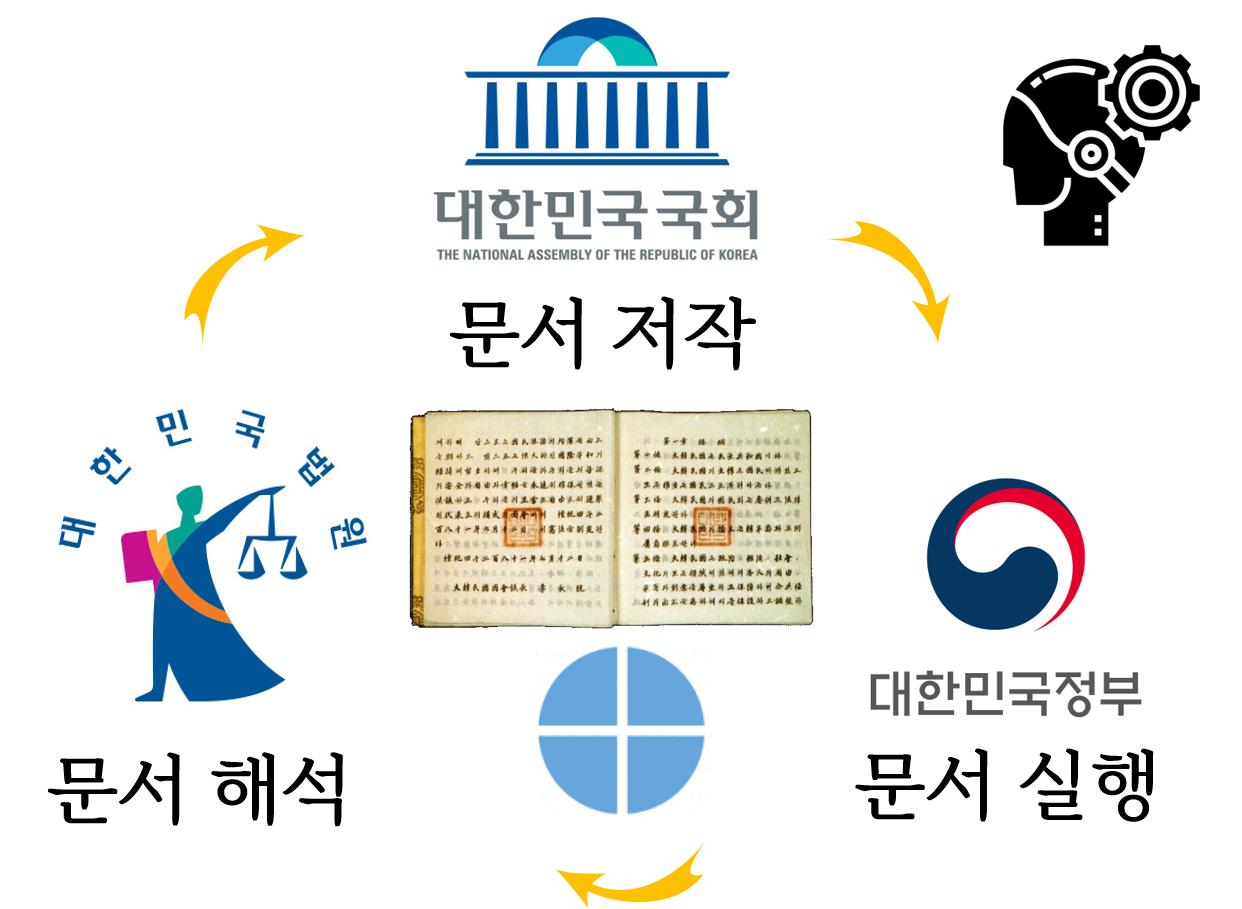
\includegraphics[width=2.84375in,height=\textheight]{images/three-pillar.png}

}

\caption{글쓰기와 삼권분립}

\end{figure}

\hypertarget{uxae00uxc4f0uxae30-uxc5eduxc0ac}{%
\section{글쓰기 역사}\label{uxae00uxc4f0uxae30-uxc5eduxc0ac}}

점토판과 쐐기를 이용한 문자 작성에서 시작하여 중세시대에는 동양에서는
붓과 머루를, 서양에서는 잉크와 새깃털펜을 사용해 저작을 했다. 타자기의
발명은 개인 저작을 가능하게 만들었고, 전동타자기의 등장은 문서 작성의
비용을 절감하고 품질을 향상시키며 출판 과정을 신속화했다. 제2차 세계대전
이후에는 군용 애니악(ENIAC) 컴퓨터가 민간에 보급되어 IBM이 1964년에 워드
프로세서를, 1969년에 저장 장치를 시장에 출시했다. 이로써 기계식 저작
방식에서 디지털 저작 방식으로 전환의 기반이 마련되었다. 1980년대 전후로
마이크로소프트 워드 1.0, 워드 퍼펙트, 아래한글과 같은 위지윅(WYSIWYG)
방식이 일반인에게 큰 인기를 끌었다면, 문서를 구조적으로 작성하여
컴파일하는 위지윔(WYSIWYM) 방식의 \href{http://example.org}{\TeX} /
\href{http://example.org}{\LaTeX} 이 비슷한 시기에 과학기술 전문가들
사이에 자리를 잡아갔다.

\begin{figure}

{\centering 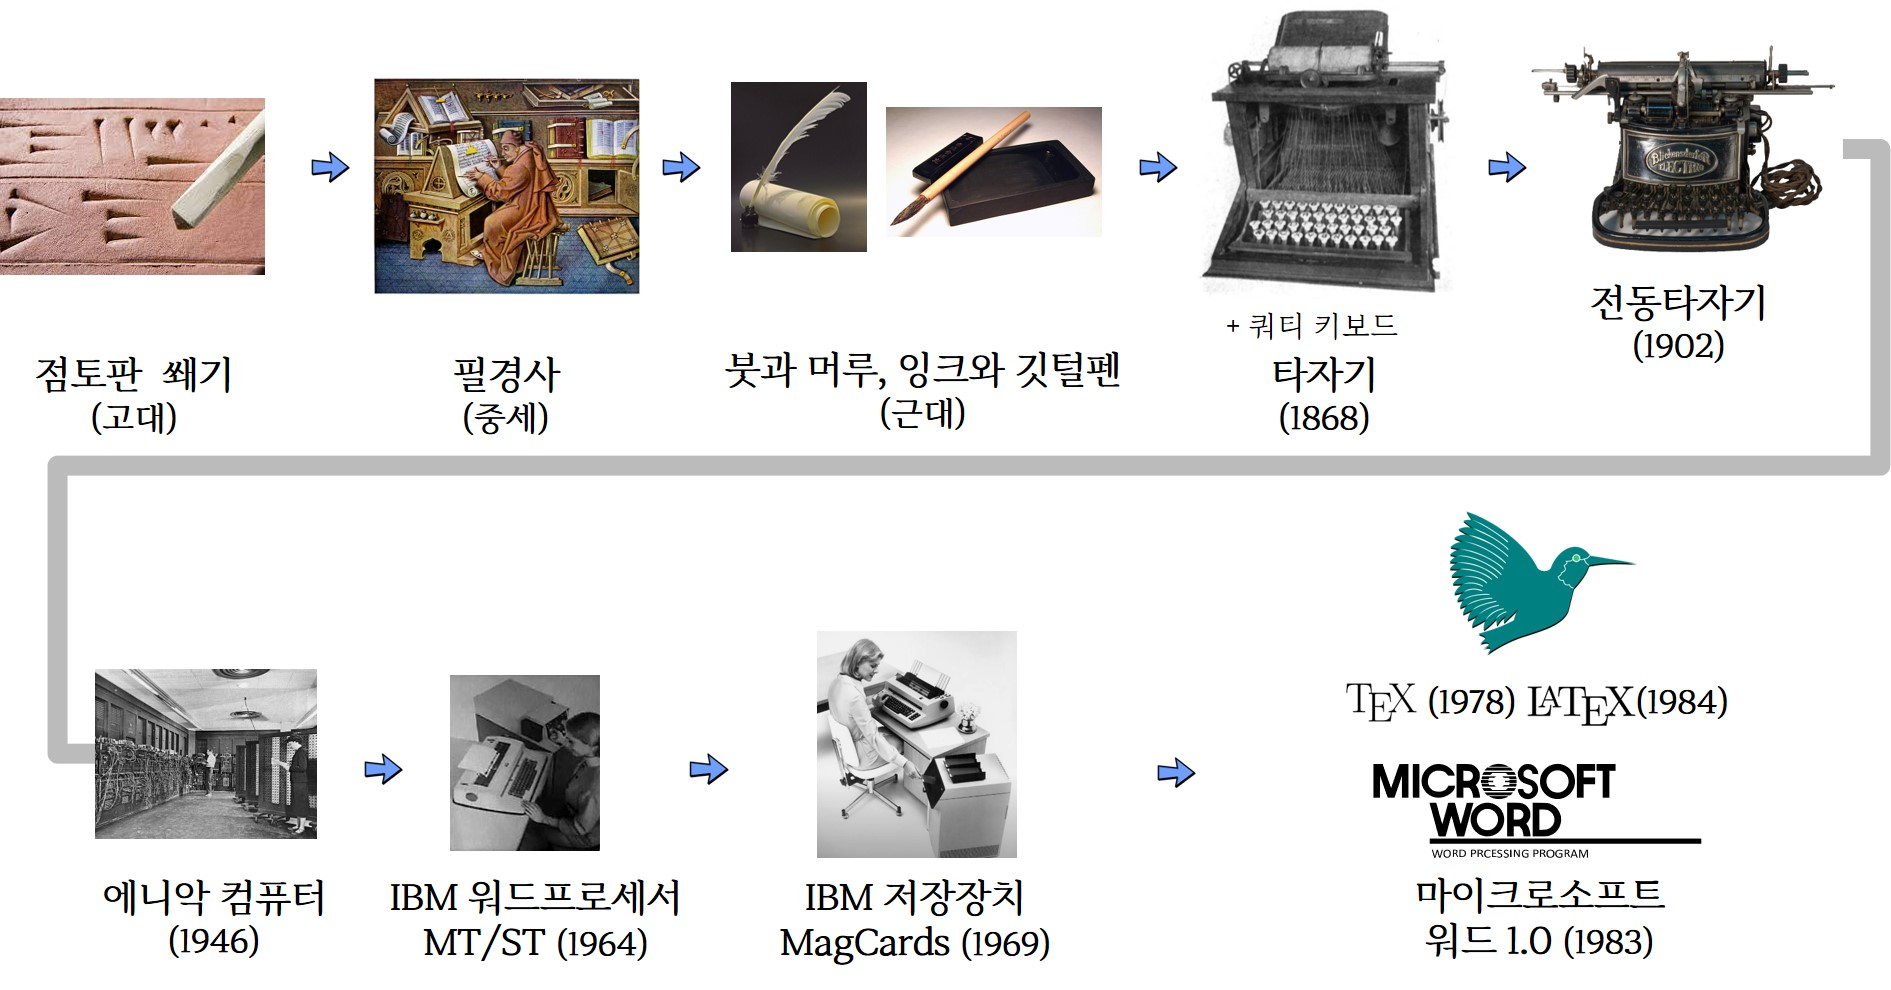
\includegraphics{images/writing-wordprocessor.jpg}

}

\caption{글쓰기 저작도구 진화과정}

\end{figure}

\hypertarget{uxbb38uxc11c-uxc800uxc791-uxd328uxb7ecuxb2e4uxc784}{%
\subsection{문서 저작
패러다임}\label{uxbb38uxc11c-uxc800uxc791-uxd328uxb7ecuxb2e4uxc784}}

아래한글이나 MS 워드 같은 워드 프로세서는 \textbf{위지위그(WYSIWYG: What
You See Is What You Get)} 방식을 기반으로 한다. 이 방식은 화면에 보이는
서식이 입혀진 텍스트가 최종 출력물과 동일하게 나오는 직관적인 특성을
가진다. 이러한 장점 덕분에 타자기나 컴파일을 필요로 하는 다른 문서 저작
방식에 비해 경쟁력을 보이며 문서 저작의 주류 소프트웨어로 자리잡았다.

반면, \textbf{위지윔(WYSIWYM: What You See Is What You Mean)} 방식의
대표적인 예는 \href{http://example.org}{\LaTeX}(레이텍)이다. 이 방식은
구조화된 형태로 문서를 작성한 후 컴파일을 통해 출판 가능한 PDF 파일을
생성한다. \href{http://example.org}{\LaTeX}의 주요 장점은 수식, 그래프,
표 등 다양한 구성요소를 미려하게 표현할 수 있다는 것이다. 또한, ``문학적
프로그래밍(literate programming)'' 패러다임을 통해 텍스트와 코드를 함께
담을 수 있고 위지위그 방식 워드프로세서 보다 문서가 복잡할수록 진가를
보여준다.

\begin{figure}

{\centering 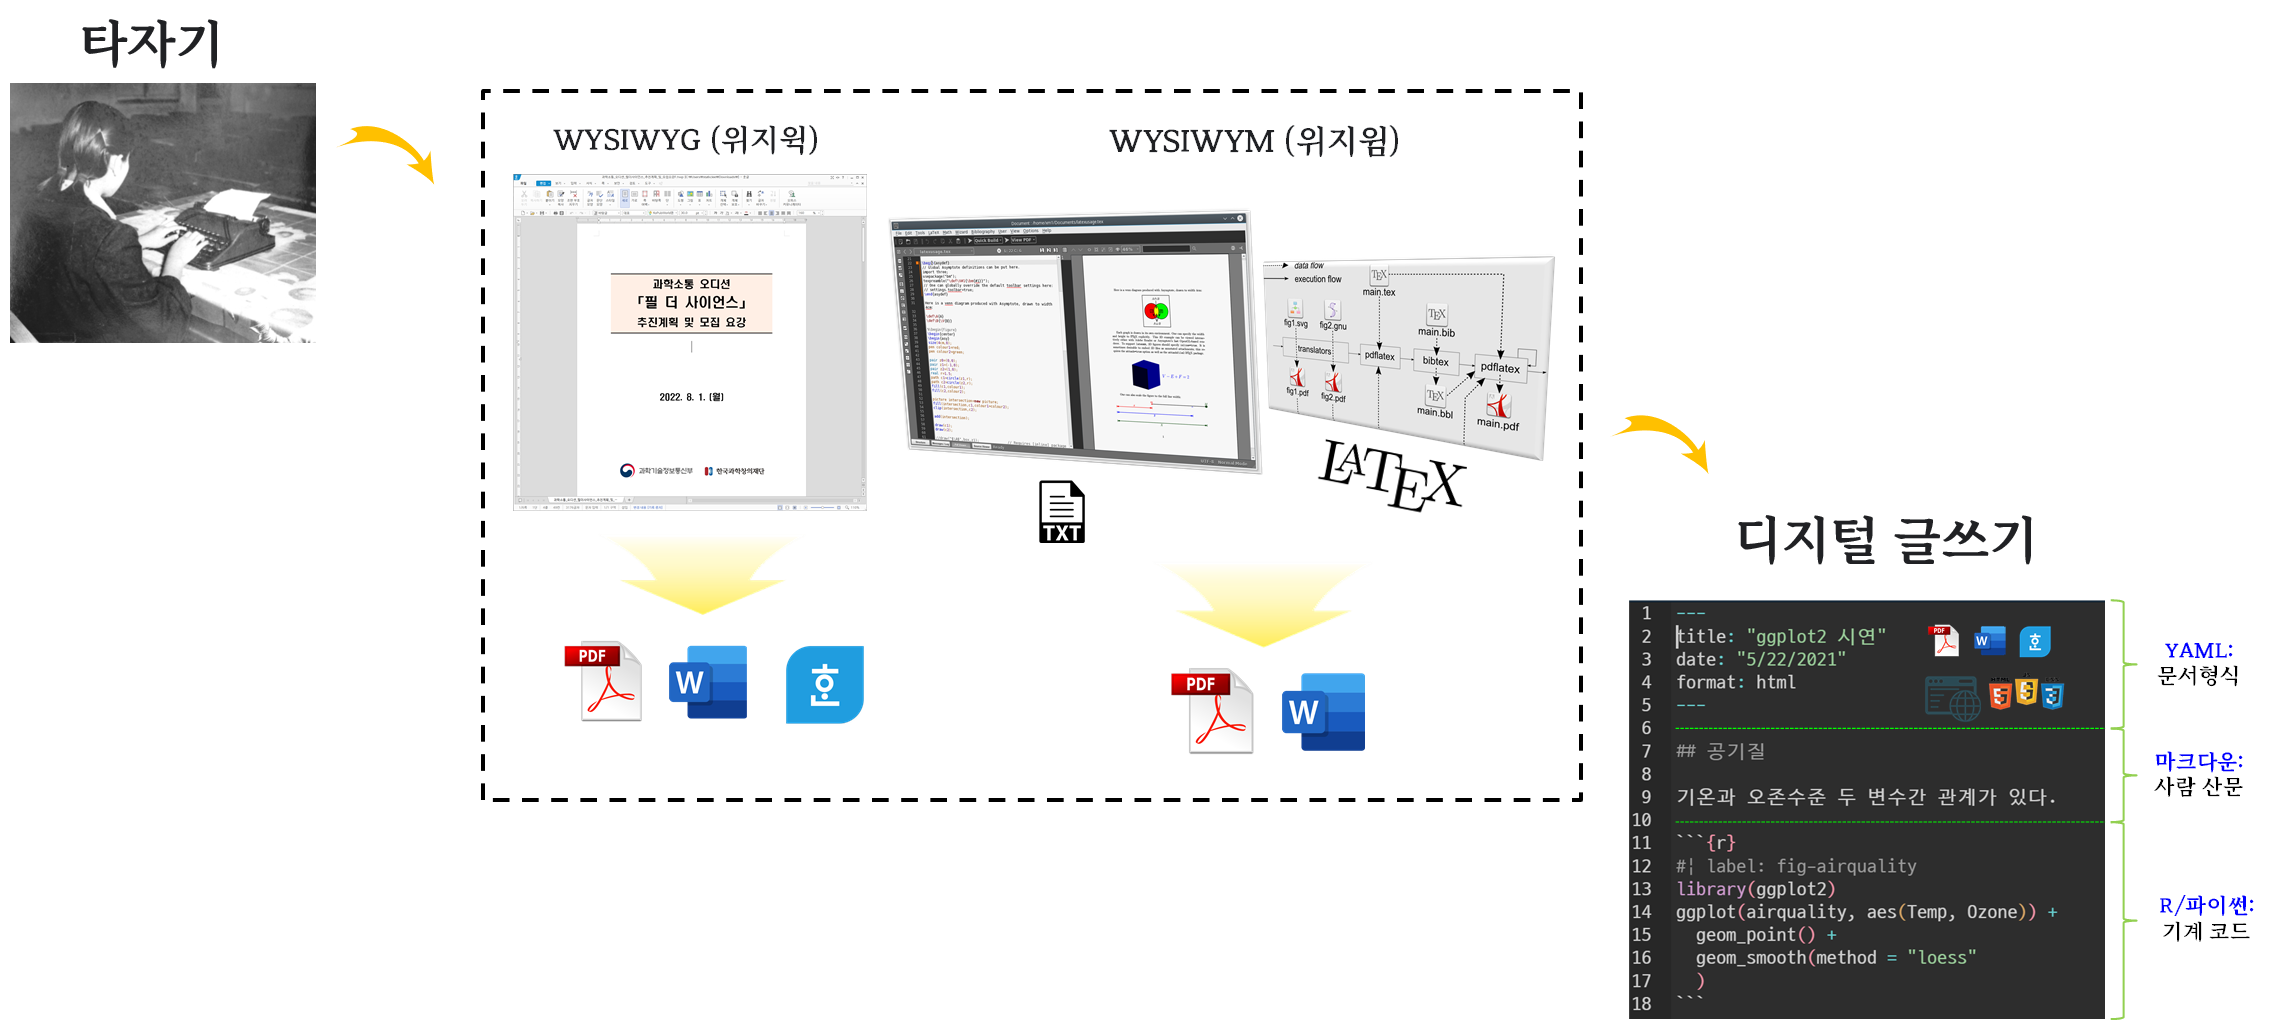
\includegraphics{images/digital-writing-paradigm-shift.png}

}

\caption{문서 저작 패러다임}

\end{figure}

최근 문서저작 도구의 패러다임은 눈에 띄는 변화를 겪고 있다. 과거에는
일반 사용자를 위한 위지위그(WYSIWYG)와 과학기술 전문가를 위한
위지윔(WYSIWYM)이라는 두 가지 주요 패러다임으로 문서저작 도구가 명확하게
구분되었다. 그러나 최근에는 챗GPT가 촉발한 생성형 AI 기술이 위지위그
패러다임에 본격적으로 도입되어, 워드프로세서부터 엑셀, 파워포인트,
데이터베이스, 프로그래밍, 그리고 멀티미디어 저작까지 다양한 분야에서
발전이 가속화되고 있다. 위지윔 패러다임도 마크다운, 팬독(pandoc),
R/Python, \href{http://example.org}{\LaTeX} 엔진 등 단위기술 발전과 함께
생성형 AI기술이 적극 반영된 RStudio, 주피터, VS코드와 같은
통합개발환경(IDE)의 발전을 통해 두 패러다임 경계가 점차 흐릿해지고 있다.

문서저작의 복잡성이 증가함에 따라 재현성, 추적성, 협업, 코딩, 버전 제어,
자동화, 생산성이 중요한 저작 요소로 부상하고 있다. 이러한 복잡한
문서저작 문제에 대한 해결책으로 문학적 프로그래밍 패러다임이 주목받고
있다.

\hypertarget{uxbb38uxc11c-uxb3c4uxad6c-uxc5eduxc0ac}{%
\subsection{문서 도구
역사}\label{uxbb38uxc11c-uxb3c4uxad6c-uxc5eduxc0ac}}

사람과 의사소통하는 텍스트와 기계와 의사소통하는 프로그래밍 언어를
작성하는 방식은 서로 다르다. 텍스트는 문서를 작성하고, 프로그래밍 언어는
코드를 작성한다는 점에서 차이가 있지만, 모두 문서를 작성한다는 점에서
공통점이 있다. 문서 작성과 코드 통합은 오래 전부터 컴퓨터 과학과 데이터
과학에서 중요한 주제였다. 그 결과 다양한 해법이 제시되고 도구도
개발되었다.

도널드 크누쓰 교수가 1978년 수식이 포함된 과학문서 작성에 특화되어
\href{http://example.org}{\TeX}를 개발하였고, 1984년 문학적 프로그래밍
개념을 제안하면서 텍스트와 코드를 섞어 문서와 프로그램을 동시에 작성할
수 있다는 것을 최초로 선보였다. 1985년에 레슬리 램포트가
\href{http://example.org}{\TeX}을 기반으로
\href{http://example.org}{\LaTeX}을 개발하여 수학과 과학 분야에서 널리
사용되는 문서저작 도구로 자리잡았다. \autocite{knuth84,spivak1990joy}
\index{\LaTeX} \index{문학적 프로그래밍}

1988년에 울프람 박사가 매쓰매티카 노트북(Mathematica Notebooks)을
개발하여 수학과 과학 연구를 위한 고급 작업 환경을 제공했지만 한동안
특별한 도구나 개념의 진전은 없었지만 2000년대 들어서면서 2001년에
페르난도 페레즈가 파이썬 대화하여 IPython을 개발했고, 2003년에
이맥스(Emacs) 텍스트 편집기에서 동작하는 작업 관리 및 문서 작성 도구인
이맥스 Org-mode를 개발했다. 2004년에 존 그루버가 웹 문서를 쉽게 작성하고
표현할 수 있는 경량 마크업 언어 마크다운(Markdown)을 공개했다.
2006년부터 본격적으로 팬독(Pandoc) 개발이 시작되면서 다양한 마크업 언어
간 자유로운 변환이 가능하게 되었다. \index{마크다운} \index{pandoc}

페르난도 페레즈는 2011년 파이썬 기반 iPython Notebook을 개발했고, 곧
이어 2012년 R 기반 \texttt{knitr} 개발이 본격화되었다. 2014년에 페르난도
페레즈가 다시 한번 다양한 프로그래밍 언어를 지원하는 주피터
프로젝트(Project Jupyter)를 주도하고 있으며, 2020년 RStudio로 잘 알려진
포짓(Posit) J.J. 알레어 대표가 과학기술 문서 작성과 데이터 과학에 특화된
쿼토(Quarto)를 개발하여 지속적으로 새로운 기능을 선보이고 있다.

\begin{longtable*}{ccc}
\toprule
연도 & 도구 & 개발자 \\ 
\midrule
1978 & TeX & Donald Knuth \\ 
1984 & Literate Programming & Donald Knuth \\ 
1988 & Mathematica Notebooks & Stephen Wolfram \\ 
2001 & IPython & Fernando Perez \\ 
2003 & Emacs org-mode & Carsten Dominik \\ 
2004 & Markdown & John Gruber \\ 
2005 & Sage Notebook & William Stein \\ 
2006 & Pandoc & John MacFarlane \\ 
2009 & GitHub Flavored Markdown & Tom Preston-Werner \\ 
2011 & iPython Notebook & Fernando Perez \\ 
2012 & knitr & Yihui Xie \\ 
2014 & Project Jupyter & Fernando Perez \\ 
2020 & 쿼토 (Quarto) & J.J. Allaire \\ 
\bottomrule
\end{longtable*}

\bookmarksetup{startatroot}

\hypertarget{uxc11cuxbb38}{%
\chapter*{서문}\label{uxc11cuxbb38}}
\addcontentsline{toc}{chapter}{서문}

\markboth{서문}{서문}

끊임없이 진화하는 인간 커뮤니케이션 환경에서 디지털 시대의 도래는 표현과
연결의 새로운 차원을 가져왔습니다. 디지털 불평등 격차해소를 추구하고
디지털 영역의 무한한 잠재력을 포용하는 작가로서, ``디지털 글쓰기''를
여러분께 소개합니다. 이 책은 창의성, 기술, 인간 정신이 융합된 공간인
디지털 글쓰기의 광활하고 길들여지지 않은 경계를 탐험하고자 하는 사람들을
위한 안내서이자 동반자 역할을 합니다.

새 시대에 등장한 다양한 플랫폼, 형식, 도구를 살펴보면서 온라인 글쓰기의
세계가 제시하는 독특한 기회와 도전 과제에 대해 자세히 살펴볼 것입니다.
이 책은 단순한 기술 매뉴얼이 아니라 말과 아이디어의 힘, 그리고 디지털
광야에 과감히 도전하는 사람들을 기다리는 무한한 가능성에 대한
찬사입니다.

디지털 시대 글쓰기 진화를 살펴보고, 스토리를 만들고, 공유하고, 소비하는
방식에 대한 기술의 혁신적인 영향을 추적하는 것으로 여정을 시작할
것입니다. 재현가능한 과학기술 문서작성과 대량생산부터 인터랙티브 서사와
멀티미디어 경험에 이르기까지 새로운 형태의 디지털 스토리텔링의 출현에
대해 논의할 것입니다.

온라인 글쓰기의 세계를 더 깊이 파고들면서 자신만의 목소리와 스타일을
개발하고, 전통적인 글쓰기 기법을 디지털 플랫폼의 고유한 요구에 맞게
조정하며, 소셜 미디어의 힘을 활용하여 독자와 소통하고 작품을 중심으로
커뮤니티를 구축하는 것의 중요성에 대해서도 살펴볼 것입니다.

익명성은 여전히 개인적인 선택이지만, 디지털 영역에서 익명성이 가져다주는
기회와 도전을 인식하는 것은 필수적입니다. 개인정보 보호와 공개성 사이의
미묘한 균형, 그리고 온라인에서 콘텐츠를 제작하고 공유할 때 고려해야 할
윤리적 고려 사항과 책임에 대해 논의할 것입니다.

디지털 글쓰기의 세계를 탐색하는 데 필요한 지식과 도구뿐만 아니라 나만의
목소리를 세상과 공유할 수 있는 영감과 용기를 얻으시기 바랍니다. 광활한
사이버 공간에 여러분의 글이 울려 퍼져 경계를 넘어 전 세계 독자들의
마음을 움직일 수 있도록 모험을 떠나보세요.

디지털 오디세이에 오신 것을 환영합니다. 모험을 시작하세요.

\bookmarksetup{startatroot}

\hypertarget{uxcc57gpt-uxae00uxc4f0uxae30-uxb9dbuxbcf4uxae30}{%
\chapter{챗GPT 글쓰기
맛보기}\label{uxcc57gpt-uxae00uxc4f0uxae30-uxb9dbuxbcf4uxae30}}

종이와 펜으로 글을 쓸 때 글쓰기는 주로 생각이나 정보, 감정을 언어의
형태로 표현하는 과정으로 가장 기본적이고 전통적인 글쓰기의 형태로 볼 수
있다. 저자가 머릿속에 있는 아이디어나 메시지를 구조화하여 문장과
단락으로 만드는 과정에서 문법, 어휘, 문장 구조 등 언어의 다양한 요소가
활용된다. 전통적인 글쓰기는 디지털 글쓰기에서 느끼기 어려운 독특한
느낌과 집중도가 있어 펜을 종이에 대고 쓰는 물리적인 행위 자체가 생각을
정리하고 창의성을 불러일으키는 경우가 많고 디지털 장비의 방해 없이 좀 더
몰입하여 글을 쓸 수 있다는 장점도 있다.

전통적인 글쓰기에서 문법, 어휘, 문장 구조 등 언어의 다양한 요소에
집중하는 이유 중 하나는 인쇄출판 비용 문제가 크다. 인쇄출판을 할 경우,
재료와 인력, 시간 등 다양한 비용이 발생하기 때문에, 처음부터 정확하고
명료한 표현을 사용하여 수정이나 재인쇄 필요성을 줄여 비용을 절감해야
하기 때문에 저자가 더 신중하게 글을 쓰도록 만들며, 그 결과로 문법이나
어휘 선택, 문장 구조 등에 더 많은 주의를 기울이게 된다. 인쇄된 글은
디지털 글과 달리 쉽게 수정할 수 없기 때문에, 처음부터 높은 수준의
정확성과 명료성이 요구되기 때문에 작성자로 하여금 더 깊게 생각하고 더
철저하게 검토하는 습관을 들이게 하며, 이러한 과정을 통해 더 높은 품질의
글이 탄생하게 되었다.

따라서, 글쓰기는 모든 사람이 배우는 기초적인 능력이지만, 인쇄출판의 높은
비용 때문에 실제로 글을 발표하고 널리 퍼뜨릴 수 있는 사람은 선택된
소수에 불과하기 때문에 빈익빈, 부익부 문제가 심해지고 있다. 즉, 자본과
기회가 있는 소수의 사람들만이 자신의 아이디어나 의견을 널리 알릴 수 있는
인쇄출판 플랫폼을 갖게 된 것이다. 이로 인해 정치적, 사회적, 경제적,
과학기술 격차가 더욱 심화되며, 다수의 목소리가 제대로 들리지 않는 문제가
발생한다. 이러한 상황은 인터넷과 웹의 대중화로 디지털 글쓰기가 보급됨에
따라 어느 정도 해소되고 있지만, 저작에 해당되는 디지털 글쓰기와 저작물의
인쇄출판과 유통에 대한 접근성 문제는 여전히 해결되어야 할 중요한 과제로
남아 있다.

\hypertarget{uxcc57gpt-uxb4f1uxc7a5}{%
\section{챗GPT 등장}\label{uxcc57gpt-uxb4f1uxc7a5}}

챗GPT 등장은 글쓰기 패러다임을 혁신적으로 바꾸고 있다. 전통적인 글쓰기는
문법, 어휘, 문장 구조 등 언어의 다양한 요소를 활용하여 아이디어나
메시지를 구조화하는 데 주력했고, 전통적인 글쓰기에서 저작은 종이와 펜,
출판은 워드 프로세서 도구로 필요한데, 디지털 도구에 익숙하지 않은
사람들에게는 글쓰기 자체가 큰 부담이 되었다.

그러나 챗GPT는 뛰어난 자연어 처리 능력 덕분에 저자는 복잡한 문법이나
어휘 없이도 자신의 생각을 쉽게 표현할 수 있을 뿐만 아니라, 챗GPT는
다양한 형태의 콘텐츠, 예를 들어 수식, 표, 그래프, 다이어그램, 코드 등을
쉽게 생성하고 편집할 수 있어, 글쓰기 범위가 전통적인 텍스트를 넘어
다양한 미디어로 확장되고 있다.

펜과 종이로 저작하여 종이 매체를 중심으로 인쇄출판이 주류를 이뤘던
시대를 워드 프로세서로 저작하여 웹사이트에 디지털 출판하는 시대로
바뀌었던 것에 비견될만큼 챗GPT는 디지털 글쓰기의 패러다임을 혁신적으로
바꾸고 있다. 챗GPT Text-to-X 기능은 글쓰기 가능성을 더욱 확장시켜 저자는
아이디어나 메시지를 표현하고 전달하는데 단순한 텍스트 입력을 넘어 수식,
그래프, 표, 다이어그램, 코드 등 다양한 형태의 콘텐츠를 쉽게 생성할 수
있게 됨에 따라, 글쓰기 경계를 훨씬 넓히게 되었다. 챗GPT 시대 누구나
복잡한 도구나 전문 지식 없이도 자신의 아이디어나 정보를 풍부하게 표현할
수 있게 되었다.

\hypertarget{uxae00uxc4f0uxae30-uxc9c4uxd654uxacfcuxc815}{%
\section{글쓰기
진화과정}\label{uxae00uxc4f0uxae30-uxc9c4uxd654uxacfcuxc815}}

글쓰기 역사는 인류 문명과 밀접하게 연결되어 있다. 고대에는 점토판과
쐐기를 사용하여 기록을 남겼다. 중세에 이르러 필경사가 등장하고, 붓과
머루, 잉크와 깃털펜이 사용되기 시작했다. 근대에 들어서면 타자기가
등장하고, 1868년에 첫 타자기가, 1902년에 전동타자기가 개발되었다.

컴퓨터 등장은 글쓰기 패러다임을 또 다시 바꾸었다. 1946년에 에니악
컴퓨터가, 1964년에 IBM 워드프로세서 MT/ST가 등장했다. 이후에는 IBM
저장장치 MagCards가 1969년에, TeX가 1978년에, LaTeX이 1984년 등장하면서
디지털 글쓰기 기술적 토대가 탄탄해졌다.

1983년에 마이크로소프트 워드 1.0의 출시로 개인용 컴퓨터에서도 글쓰기가
가능해지면서 디지털 글쓰기의 새로운 시대가 열렸다. 그 후로 프로그래밍
언어와 글쓰기가 통합되기 시작했고, 마크다운, R, 파이썬 등을 활용한
글쓰기가 일반화되면서 문학적 프로그래밍(Literate Programming)이라는
새로운 형태의 글쓰기를 가능하게 했다. 최근에는 챗GPT의 등장으로 문학적
프로그래밍이 한 단계 더 진화하고 있다. 챗GPT는 자연어 처리 능력을
활용하여 코드와 텍스트, 그리고 다양한 미디어 요소를 통합적으로 다룰 수
있어, 디지털 글쓰기의 패러다임을 혁신적으로 바꾸고 있다.

\begin{figure}

{\centering 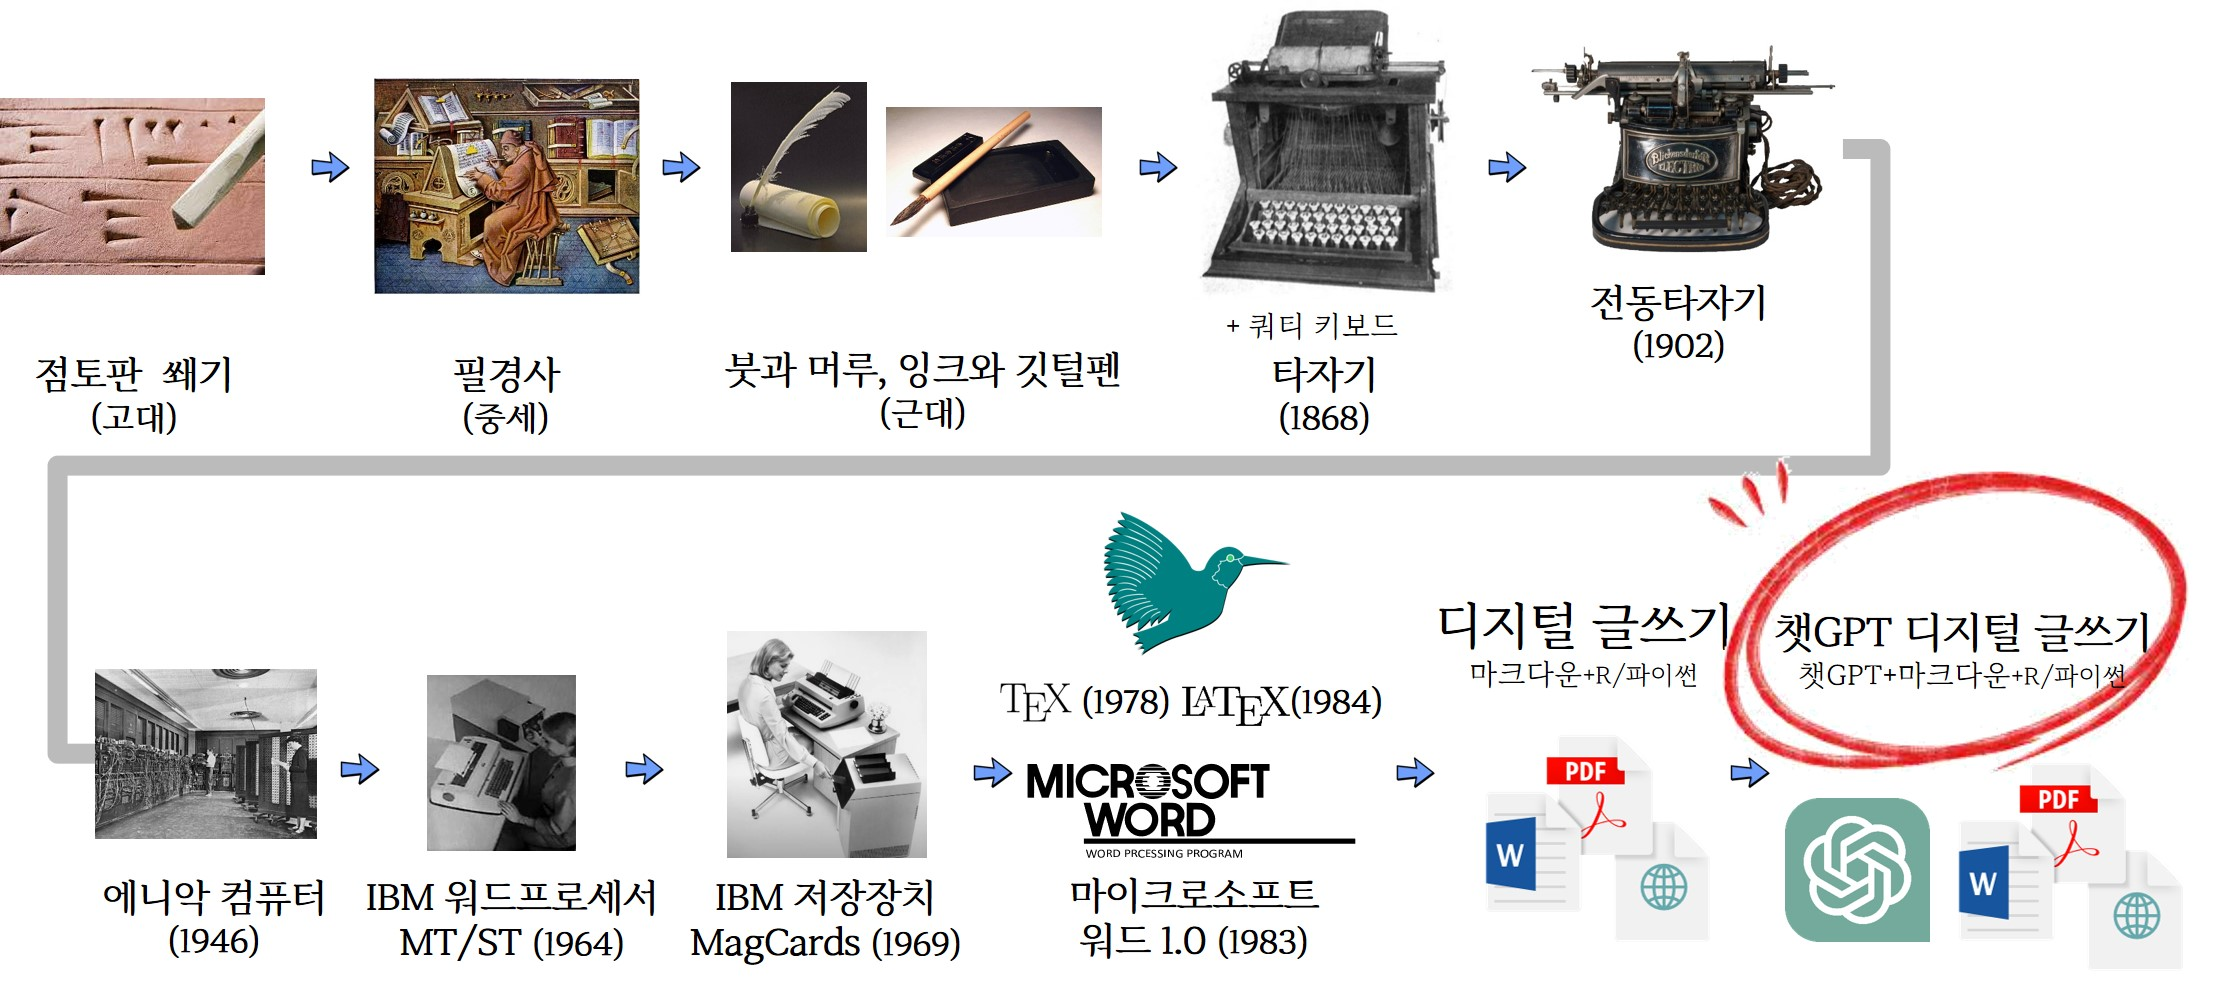
\includegraphics{images/writing_history.jpg}

}

\caption{챗GPT 디지털 글쓰기 진화과정}

\end{figure}

\hypertarget{uxae00uxc4f0uxae30-uxc791uxc5c5uxd750uxb984}{%
\section{글쓰기
작업흐름}\label{uxae00uxc4f0uxae30-uxc791uxc5c5uxd750uxb984}}

챗GPT 디지털 글쓰기의 일반적인 작업흐름은 더 세분화할 수 있지만,
``디지털 글쓰기'', ``구조와 외양'', ``배포와 공유''로 구분할 수 있다.

첫 번째 단계인 ``디지털 글쓰기''에서는 글감을 시작점으로 하여 다양한
형태의 콘텐츠를 생성하는데 수식, 표, 그래프, 파이썬/R/SQL 코드, 그림,
도형 등이 포함된다. 자연어로 챗GPT를 통해 다양한 저작물 구성요소를 쉽고
빠르게 생성하고 편집할 수 있다.

두 번째 단계인 ``구조와 외양''에서 문서의 전반적인 구조와 서식을
결정한다. 문서의 구조, 서식, 레이아웃, 그리고 참조 등이 확립되는데 챗GPT
부조종사(Copilot)이 유령 텍스트(Ghost Text) 기능을 통해 자연어로 저자
작업을 더욱 효율적으로 지원한다.

마지막 단계인 ``배포와 공유''에서 작성된 저작물이 독자에게 다양한 매체를
통해 전달한다. 독자가 반듯이 사람일 필요는 없고 독자가 저작자 자신일
수도 있으며, 심지어 기계일 수도 있다. 챗GPT 배포와 공유 과정에서
발생되는 다양한 기술적 문제를 해결해주는 공동 저작자이자 동료로서 디지털
글쓰기 전체적인 흐름을 완성한다.

\begin{figure}[H]

{\centering \includegraphics[width=11.2in,height=6.67in]{whole_game_files/figure-latex/mermaid-figure-1.png}

}

\end{figure}

\hypertarget{uxcc57gpt-uxb514uxc9c0uxd138-uxae00uxc4f0uxae30-uxc0acuxb840}{%
\section{챗GPT 디지털 글쓰기
사례}\label{uxcc57gpt-uxb514uxc9c0uxd138-uxae00uxc4f0uxae30-uxc0acuxb840}}

사전 자료조사를 통해서 한국영화 10선 중 \textbf{국제시장}과
\href{https://r2bit.com/chatGPT/palmer_penguins.html}{펭귄 데이터}를
통해 흥행과 동시에 현재 당면한 ESG 문제를 다룬 뭉클한 감동을 주는 영화
시놉시스 작성을 목표로 하는 저작물을 작성해보자.

챗GPT 디지털 글쓰기를 활용하여 영화 시놉시스를 작성하는 과정은 다음과
같다.

\begin{enumerate}
\def\labelenumi{\arabic{enumi}.}
\item
  \textbf{디지털 글쓰기 단계}: 먼저, ``국제시장''과 ``펭귄 데이터''를
  통해 얻은 글감을 바탕으로 영화의 주제와 구조를 설정한다. 챗GPT를
  사용하여 흥행 가능성과 ESG 문제에 대한 데이터를 분석하여 표와 그래프로
  시각화한다.
\item
  \textbf{구조와 외양 단계}: 시놉시스 구조를 결정하고, 적절한 서식과
  레이아웃을 적용한다. 문서 참조나 인용 등 챗GPT를 활용하여 자연어로
  쉽게 추가할 수 있다.
\item
  \textbf{배포와 공유 단계}: 작성된 시놉시스를 다양한 플랫폼과 매체를
  통해 공유한다. 디지털 출판 배포과정에서 챗GPT는 기술적 문제를 해결함은
  물론 방향도 제시하여 독자가 사람이든 기계든 쉽게 출판저작물에 접근할
  수 있도록 지원한다.
\end{enumerate}

목표한 ``영화 시놉시스''를 챗GPT 디지털 글쓰기로 작업한 결과물은 다음과
같이 복잡한 데이터 분석부터 감동적인 내러티브까지 한 번에 작업할 수
있다.

\begin{quote}
영화 제목을 ``펭귄의 꿈: ESG로 미래를 바꾸다''로 설정하고, 주인공은
한국에서 ESG 문제에 관심을 가진 젊은 연구원으로 한다. 그는 남극의 펭귄
데이터를 분석하여 지구의 미래를 예측하고, 이를 통해 사람들에게 ESG의
중요성을 알리려고 한다. 영화는 그의 여정과 성장, 그리고 마침내 세계를
바꾸는 뭉클한 결말로 끝난다.
\end{quote}

\begin{figure}[H]

{\centering \includegraphics[width=9.15in,height=5.73in]{whole_game_files/figure-latex/mermaid-figure-3.png}

}

\end{figure}

\hypertarget{uxcc57gpt-uxae00uxac10-uxc791uxc131}{%
\subsection{챗GPT 글감 작성}\label{uxcc57gpt-uxae00uxac10-uxc791uxc131}}

실제 데이터가 필요한 경우 영화진흥위원회에서 매년 발표하는
``한국영화연감''의 영화별 흥행기록
\href{https://www.kobis.or.kr/kobis/business/stat/offc/findFormerBoxOfficeList.do}{역대
박스오피스 (공식통계 기준)}에서 정확한 데이터를 확인할 수 있다. 챗GPT는
프롬프트에 대한 답변을 생성하는 언어 모형으로 챗GPT는 데이터베이스나
실시간 정보에 접근하지 않고 기존에 학습된 데이터를 기반으로 답변을
제공한다. 따라서, 100\% 사실은 아니지만 빠르게 답변을 제공받아 시놉시스
제작에 활용하는 경우 대략 8\textasciitilde90\% 정확도를 보이는 업무에
챗GPT 활용은 가능하다. 예를 들어, ``관람객 기준으로 가장 많은 관람객을
갖는 한국 영화 상위 5개 알려주세요''라는 프롬프트에 대한 답변을 챗GPT로
받아 다음과 같이 마크다운 형태로 가공하여 후속 작업에 활용한다.

\begin{tcolorbox}[enhanced jigsaw, opacityback=0, opacitybacktitle=0.6, colback=white, rightrule=.15mm, coltitle=black, colframe=quarto-callout-note-color-frame, colbacktitle=quarto-callout-note-color!10!white, bottomrule=.15mm, bottomtitle=1mm, breakable, title=\textcolor{quarto-callout-note-color}{\faInfo}\hspace{0.5em}{프롬프트}, titlerule=0mm, leftrule=.75mm, toptitle=1mm, left=2mm, arc=.35mm, toprule=.15mm]

\begin{quote}
관람객 기준으로 가장 많은 관람객을 갖는 한국 영화 상위 5개 알려주세요
시놉시스는 200자 길이로 작성해주세요. 출력형식은 다음과 같은 형태로
마크다운 소스파일 형태로 출력해 주세요.

\textbar 순위\textbar 영화명\textbar{}
연도\textbar 감독\textbar 배급사\textbar 관객수\textbar 시놉시스\textbar{}
\end{quote}

\hypertarget{uxcd9cuxb825uxacb0uxacfc}{%
\subsubsection*{출력결과}\label{uxcd9cuxb825uxacb0uxacfc}}
\addcontentsline{toc}{subsubsection}{출력결과}

죄송합니다, 제 정보는 2021년 9월까지로 제한되어 있어서 그 이후의
데이터에 대한 정확한 정보를 제공할 수 없습니다. 그러나, 2021년 9월까지
기준으로 가장 많은 관람객을 가진 한국 영화 상위 5개는 다음과 같습니다.

\begin{longtable}[]{@{}
  >{\centering\arraybackslash}p{(\columnwidth - 12\tabcolsep) * \real{0.0750}}
  >{\centering\arraybackslash}p{(\columnwidth - 12\tabcolsep) * \real{0.1000}}
  >{\centering\arraybackslash}p{(\columnwidth - 12\tabcolsep) * \real{0.0750}}
  >{\centering\arraybackslash}p{(\columnwidth - 12\tabcolsep) * \real{0.1000}}
  >{\centering\arraybackslash}p{(\columnwidth - 12\tabcolsep) * \real{0.1000}}
  >{\centering\arraybackslash}p{(\columnwidth - 12\tabcolsep) * \real{0.1125}}
  >{\centering\arraybackslash}p{(\columnwidth - 12\tabcolsep) * \real{0.4375}}@{}}
\toprule\noalign{}
\begin{minipage}[b]{\linewidth}\centering
순위
\end{minipage} & \begin{minipage}[b]{\linewidth}\centering
영화명
\end{minipage} & \begin{minipage}[b]{\linewidth}\centering
연도
\end{minipage} & \begin{minipage}[b]{\linewidth}\centering
감독
\end{minipage} & \begin{minipage}[b]{\linewidth}\centering
배급사
\end{minipage} & \begin{minipage}[b]{\linewidth}\centering
관객수
\end{minipage} & \begin{minipage}[b]{\linewidth}\centering
시놉시스
\end{minipage} \\
\midrule\noalign{}
\endhead
\bottomrule\noalign{}
\endlastfoot
1 & 명량 & 2014 & 김한민 & 씨제이이앤엠 & 1761만 & 1592년 임진왜란, 이때
조선은 거대한 전쟁의 중심에 있었다. 여기에서 조선 최고의 장군 이순신이
일어나 대역적인 전투를 벌인다. \\
2 & 극한직업 & 2019 & 이병헌 & 씨제이이앤엠 & 1626만 & 각종 범죄
현장에서 물리적인 고난과 위험을 감수하며 사건을 해결하는 특수 대원들의
이야기. 그러나 그들의 직업은 상상을 초월하는 극한의 직업, 치킨집
사장이었다. \\
3 & 신과함께-인과 연 & 2018 & 김용화 & 롯데엔터테인먼트 & 1441만 &
살아있는 동안 저지른 죄에 대해 사후세계에서 재판을 받는 과정을 그린
영화. 사망 후 49일 동안 7개의 지옥에서 7번의 재판을 받아야 하는데, 이
과정을 수행하는 천사들의 이야기. \\
4 & 국제시장 & 2014 & 윤제균 & 씨제이엔터테인먼트 & 1426만 & 한국 전쟁을
배경으로 한 영화로, 한 남자가 가족을 지키고, 살아남기 위해 펼쳐나가는
감동적인 사랑과 희망의 이야기를 담고 있다. \\
5 & 어벤져스: 엔드게임 & 2019 & 안소니 루소, 조 루소 & 월트 디즈니
코리아 & 1393만 & 타노스에 의해 절반의 생명이 사라진 채 패배한 어벤져스.
남은 멤버들은 어떻게든 가족과 친구들을 다시 데려오기 위한 모든 것을 걸고
마지막 전투에 나선다. \\
\end{longtable}

\end{tcolorbox}

\hypertarget{uxc2e4uxc81c-uxb370uxc774uxd130}{%
\subsubsection{실제 데이터}\label{uxc2e4uxc81c-uxb370uxc774uxd130}}

챗GPT는 2021년 9월까지 실제 인터넷에 공개된 데이터를 바탕으로 학습한
언어모형이다. 따라서 최신 데이터는 반영하지 못하고 과거 학습한 데이터도
모든 과거를 대표하는 것도 아니다. 잘 작성된 프롬프트를 챗GPT 언어모형과
결합하여 나온 텍스트는 100\% 사실이 아니지만 대략적인 흐름을 파악하는
데는 충분하다. 영화진흥위원에서 매년 발표하는 ``한국영화연감''의 영화별
흥행기록
\href{https://www.kobis.or.kr/kobis/business/stat/offc/findFormerBoxOfficeList.do}{역대
박스오피스 (공식통계 기준)}에서 통계적으로 정확한 한국 영화 10개를
뽑아보면 대략 일치함을 확인할 수 있다. 시간이 지나면서 챗GPT에 대한
활용이 늘어나고 언어모형이 고도화되면 이러한 통계적인 정확도는 더욱
높아질 것으로 보인다.

\begin{longtable*}{clcccll}
\toprule
순위 & 영화명 & 개봉일 & 매출액 & 관객수 & 국적 & 배급사 \\ 
\midrule
1 & 명량 & 1406646000 & $1,357$ & $1,761$ & 한국 & (주)씨제이이엔엠 \\ 
2 & 극한직업 & 1548169200 & $1,396$ & $1,626$ & 한국 & (주)씨제이이엔엠 \\ 
3 & 신과함께-죄와 벌 & 1513695600 & $1,157$ & $1,441$ & 한국 & 롯데쇼핑㈜롯데엔터테인먼트 \\ 
4 & 국제시장 & 1418742000 & $1,109$ & $1,426$ & 한국 & (주)씨제이이엔엠 \\ 
5 & 어벤져스: 엔드게임 & 1556031600 & $1,222$ & $1,393$ & 미국 & 월트디즈니컴퍼니코리아 \\ 
6 & 겨울왕국 2 & 1574262000 & $1,148$ & $1,375$ & 미국 & 월트디즈니컴퍼니코리아 \\ 
7 & 아바타 & 1260975600 & $1,284$ & $1,362$ & 미국 & 해리슨앤컴퍼니,이십세기폭스코리아(주) \\ 
8 & 베테랑 & 1438700400 & $1,052$ & $1,341$ & 한국 & (주)씨제이이엔엠 \\ 
9 & 괴물 & 1153926000 & $0$ & $1,302$ & 한국 & (주)쇼박스 \\ 
10 & 도둑들 & 1343142000 & $937$ & $1,298$ & 한국,홍콩 & (주)쇼박스 \\ 
\bottomrule
\end{longtable*}

\hypertarget{uxd3aduxadc4-uxb370uxc774uxd130uxc14b}{%
\subsubsection{펭귄
데이터셋}\label{uxd3aduxadc4-uxb370uxc774uxd130uxc14b}}

미국에서 ``George Floyd''가 경찰에 의해 살해되면서 촉발된
\href{https://ko.wikipedia.org/wiki/Black_Lives_Matter}{``Black Lives
Matter''} 운동은 아프리카계 미국인을 향한 폭력과 제도적 인종주의에
반대하는 사회운동이다. 한국에서도 소수 정당인 정의당에서 기사로 낼
정도로 적극적으로 나서고 있다.\footnote{\href{http://www.hani.co.kr/arti/politics/assembly/949422.html}{정환봉
  기자 (2020-06-15), ``여당 의원 176명 중 누가?\ldots 차별금지법 발의할
  '의인'을 구합니다'', 한겨레 신문}}

데이터 과학에서 최근 R.A. Fisher의 과거 저술한 ``The genetical theory of
natural selection'' \autocite{edwards2000genetical} 우생학(Eugenics)
대한 관점이 논란이 되면서 R 데이터 과학의 첫 데이터셋으로 그가
만들었다고 하는 붓꽃 \texttt{iris} 데이터를 대안적 데이터, 즉 펭귄
데이터로 대체하는 움직임이 활발히 전개되고 있다.
\href{https://github.com/allisonhorst/palmerpenguins}{\texttt{palmerpenguins}}
\autocite{penguin2020} 데이터셋이 대안으로 많은 호응을 얻고 있다.
\autocite{AbdulMajedRaja2020}, \autocite{Levy2019} \index{R.A. Fisher}
\index{붓꽃 데이터셋} \index{펭귄 데이터셋}

\hypertarget{uxc2dcuxb189uxc2dcuxc2a4-uxc0dduxc131}{%
\subsubsection{시놉시스
생성}\label{uxc2dcuxb189uxc2dcuxc2a4-uxc0dduxc131}}

챗GPT를 활용하면 더욱 정교하고 창의적인 답변 및 콘텐츠를 제작할 수 있다.
예시로 ``영화의 시놉시스와 펭귄에 관한 데이터를 결합하여 새로운 영화
시놉시스를 구성해 주세요''라는 프롬프트는 챗GPT에게 서로 다른 주제를
통합해 새로운 작품 시놉시스 제작을 지시내린다. 챗GPT는 제공된 프롬프트를
분석하고 이해한 뒤 새로운 시놉시스를 만들어 낸다. 특히 눈에 띄는 점은
챗GPT가 새로운 시놉시스를 대략 10초 이내 빠르게 생성한다는 것이다.

\begin{tcolorbox}[enhanced jigsaw, opacityback=0, opacitybacktitle=0.6, colback=white, rightrule=.15mm, coltitle=black, colframe=quarto-callout-note-color-frame, colbacktitle=quarto-callout-note-color!10!white, bottomrule=.15mm, bottomtitle=1mm, breakable, title=\textcolor{quarto-callout-note-color}{\faInfo}\hspace{0.5em}{프롬프트}, titlerule=0mm, leftrule=.75mm, toptitle=1mm, left=2mm, arc=.35mm, toprule=.15mm]

\begin{quote}
영화 시놉시스와 펭귄 데이터가 백틱(```)으로 감싸져 있습니다. 다음 영화
시놉시스와 데이터를 하나로 합하여 전혀 새로운 영화 시놉시스를
작성해주세요.

``` 첫번째 영화: 국제시장

덕수(황정민)의 가족은 흥남 철수 때 부산 국제시장에 내려온 피난민이다.
전쟁통에 아버지를 잃은 덕수는 졸지에 어머니와 두 동생의 생계를 책임지게
됐다. 동생의 학비와 생활비를 벌기 위해 자신의 꿈을 버린 채 친구
달구(오달수)와 함께 서독의 탄광으로, 베트남전으로 뛰어들어야 했던 덕수.
덕분에 사랑하는 아내 영자(김윤진)를 만날 수 있었고, 토끼 같은 자식들을
대학에 보낼 수 있었지만, 그의 인생에서 '그'는 한번도 없었다.

데이터: 펭귄 데이터

이 데이터는 미국 장기 생태 연구 네트워크의 일부인 파머 스테이션 장기
생태 연구 프로그램의 크리스틴 고먼 박사가 2007년부터 2009년까지 수집한
것입니다. 이 데이터는 환경 데이터 이니셔티브(EDI) 데이터 포털에서 직접
가져온 것으로, 팔머 스테이션 데이터 정책에 따라 CC0 라이선스(``권리
없음'')로 사용할 수 있습니다. ```

\hypertarget{uxc751uxb2f5}{%
\subsubsection*{응답}\label{uxc751uxb2f5}}
\addcontentsline{toc}{subsubsection}{응답}

새로운 영화 시놉시스:
\end{quote}

\hypertarget{uxc751uxb2f5-1}{%
\subsubsection*{응답}\label{uxc751uxb2f5-1}}
\addcontentsline{toc}{subsubsection}{응답}

\textbf{새로운 영화: ``펭귄의 꿈''}

덕수(황정민)는 부산 국제시장에서 가족을 부양하며 살아가는 평범한
사람이었다. 그러나 그의 가족은 흥남 철수 때 피난민으로 내려온
펭귄들이었다. 덕수는 아버지를 잃은 후, 어머니와 두 동생 펭귄의 생계를
책임지게 되었다.

덕수는 동생 펭귄들의 학비와 생활비를 벌기 위해 자신의 꿈을 포기하고,
친구 달구(오달수)와 함께 미국 장기 생태 연구 네트워크의 일부인 파머
스테이션으로 떠나게 된다. 그곳에서 그는 크리스틴 고먼 박사와 함께
2007년부터 2009년까지 펭귄 데이터를 수집하는 일을 하게 된다.

덕수의 노력 덕분에 사랑하는 아내 영자(김윤진)와 펭귄 동생들을 대학에
보낼 수 있었다. 그러나 그의 인생에서 '그'는 한번도 없었다. 그는 항상
펭귄들을 위해 자신을 희생하며 살아갔다. 그러나 그의 꿈은 언제나 그의
마음속에 살아있었다. 그의 꿈은 펭귄들이 자유롭게 날아다닐 수 있는 세상을
만드는 것이었다. 그의 이야기는 우리에게 희망과 용기, 그리고 사랑에 대한
진정한 의미를 가르쳐준다.

\textbf{새로운 영화: ``펭귄의 꿈''}

덕수(황정민)는 부산 국제시장에서 가족을 부양하는 평범한 사람이었다. 그는
전쟁으로 아버지를 잃고, 어머니와 두 동생의 생계를 책임지며, 친구
달구(오달수)와 함께 서독의 탄광과 베트남전으로 뛰어들어야 했다. 그럼에도
불구하고 그는 사랑하는 아내 영자(김윤진)를 만나고, 자식들을 대학에 보낼
수 있었다.

그러던 어느 날, 덕수는 크리스틴 고먼 박사의 펭귄 연구 데이터를 우연히
발견하게 된다. 이 데이터는 2007년부터 2009년까지 미국 장기 생태 연구
네트워크의 일부인 파머 스테이션에서 수집된 것이었다. 덕수는 이 데이터를
통해 펭귄들의 생태와 생활 패턴에 대해 알게 되고, 그들의 삶에 깊은 관심을
갖게 된다.

덕수는 자신의 삶과 펭귄들의 삶을 비교하며, 그들이 겪는 어려움과 도전에
공감하게 된다. 그는 펭귄들의 삶을 이해하고 보호하려는 새로운 꿈을 갖게
되고, 그 꿈을 이루기 위해 자신의 모든 것을 바치기로 결심한다. 이제
덕수의 새로운 도전이 시작되는데\ldots{}

덕수는 펭귄들의 생태를 연구하며 그들이 겪는 환경적 위협에 대해 알게
된다. 특히, 기후 변화와 인간의 활동이 펭귄들의 서식지를 위협하고 있다는
사실에 충격을 받는다. 그는 이 문제를 해결하기 위해 자신의 모든 것을
바치기로 결심한다.

덕수는 달구와 함께 펭귄 보호 운동을 시작한다. 그들은 펭귄들의 서식지를
보호하고, 인간의 활동이 펭귄들에게 미치는 영향을 줄이기 위한 다양한
활동을 벌인다. 이 과정에서 덕수는 자신의 삶에 새로운 의미와 목표를 찾게
된다.

덕수의 펭귄 보호 운동은 점차 사람들의 주목을 받게 된다. 그의 노력은 많은
사람들에게 영감을 주고, 점차 많은 사람들이 펭귄 보호 운동에 참여하게
된다. 그러나 동시에, 그의 활동은 기업의 이익을 위협하며, 그에게 많은
도전과 위협을 가져다준다.

그러나 덕수는 자신의 꿈을 포기하지 않는다. 그는 펭귄들의 삶을 보호하기
위해 끝까지 싸우기로 결심한다. 그의 노력은 결국 성공하게 되고, 펭귄들의
서식지는 보호되게 된다.

``펭귄의 꿈''은 평범한 사람이 어떻게 자신의 꿈을 이루고, 세상을 바꿀 수
있는지를 보여주는 영화다. 이 영화는 우리에게 꿈을 이루기 위한 도전과
희생, 그리고 그 과정에서 얻는 성취와 만족감에 대해 생각하게 한다.

\textbf{영화 제목: ``펭귄의 시장''}

미국 장기 생태 연구 네트워크의 일부인 파머 스테이션에서 크리스틴 고먼
박사(김윤진)는 2007년부터 2009년까지 펭귄에 대한 연구를 수행하였다.
그녀의 연구는 펭귄의 생태계와 그들의 생존 전략에 대한 깊은 이해를
제공하였다.

한편, 부산 국제시장에서 살아가는 덕수(황정민)는 전쟁으로 아버지를 잃고,
어머니와 두 동생의 생계를 책임지게 된다. 그는 동생의 학비와 생활비를
벌기 위해 자신의 꿈을 버리고 친구 달구(오달수)와 함께 미국으로 떠나게
된다. 그의 목적지는 바로 크리스틴 박사가 연구를 수행하는 파머
스테이션이다.

덕수는 파머 스테이션에서 일하면서 크리스틴 박사와 사랑에 빠지게 되고,
그녀의 연구에도 도움을 주게 된다. 그는 펭귄의 생존 전략을 배우며, 그것이
자신의 삶에 어떻게 적용될 수 있는지를 깨닫게 된다. 그의 인생에서 '그'는
한번도 없었지만, 펭귄들과의 만남을 통해 그는 새로운 꿈과 희망을 찾게
된다.

``펭귄의 시장''은 생존과 사랑, 그리고 꿈을 찾아가는 이들의 이야기를
그린다.

\textbf{영화 제목: ``펭귄의 꿈''}

2007년부터 2009년까지 미국 장기 생태 연구 네트워크의 일부인 파머
스테이션에서 활동한 크리스틴 고먼 박사(김윤진)는 펭귄의 생태계에 대한
깊은 이해를 가지고 있다. 그녀의 연구는 펭귄의 생존 전략과 그들의 환경에
대한 중요한 정보를 제공한다.

한편, 부산 국제시장에서 살아가는 덕수(황정민)는 전쟁으로 아버지를 잃고,
어머니와 두 동생의 생계를 책임지게 된다. 그는 동생들의 학비와 생활비를
벌기 위해 자신의 꿈을 포기하고, 친구 달구(오달수)와 함께 미국으로 떠나게
된다. 그의 목적지는 바로 크리스틴 박사가 연구를 수행하는 파머
스테이션이다.

덕수는 파머 스테이션에서 일하면서 크리스틴 박사와 사랑에 빠지게 되고,
그녀의 연구에도 도움을 주게 된다. 그는 펭귄의 생존 전략을 배우며, 그것이
자신의 삶에 어떻게 적용될 수 있는지를 깨닫게 된다. 그의 인생에서 '그'는
한번도 없었지만, 펭귄들과의 만남을 통해 그는 새로운 꿈과 희망을 찾게
된다.

``펭귄의 꿈''은 생존과 사랑, 그리고 꿈을 찾아가는 이들의 이야기를
그린다. 이 영화는 인간의 삶과 펭귄의 생존 전략 사이의 유사성을 통해 우리
모두가 어떻게 살아가야 하는지에 대한 깊은 메시지를 전달한다.

\textbf{영화 제목: ``데이터의 시장''}

덕수(황정민)는 부산 국제시장에서 가족을 부양하며 살아가는 평범한
사람이었다. 그의 가족은 흥남 철수 때 피난민으로 내려온 사람들이었다.
아버지를 잃은 후, 어머니와 두 동생의 생계를 책임지게 된 덕수는 그들의
생활비를 벌기 위해 자신의 꿈을 포기하고, 친구 달구(오달수)와 함께 미국의
데이터 연구소로 떠나게 된다.

데이터 연구소에서 그는 크리스틴 고먼 박사와 함께 2007년부터 2009년까지
펭귄 데이터를 수집하는 일을 하게 된다. 이 과정에서 덕수는 데이터 분석의
중요성과 그것이 어떻게 세상을 바꿀 수 있는지를 깨닫게 된다.

덕수의 노력 덕분에 사랑하는 아내 영자(김윤진)와 동생들을 대학에 보낼 수
있었다. 그러나 그의 인생에서 '그'는 한번도 없었다. 그는 항상 가족들을
위해 자신을 희생하며 살아갔다. 그러나 그의 꿈은 언제나 그의 마음속에
살아있었다. 그의 꿈은 데이터를 통해 세상을 바꾸는 것이었다.

``데이터의 시장''은 우리에게 희망과 용기, 그리고 사랑에 대한 진정한
의미를 가르쳐준다. 이 영화는 우리에게 자신을 희생하며 가족을 위해
살아가는 덕수의 이야기를 통해, 가족의 사랑과 헌신, 그리고 데이터의 힘에
대해 생각하게 한다.

\textbf{영화 제목: ``펭귄 데이터의 미스터리''}

덕수(황정민)는 부산 국제시장에서 가족을 부양하며 살아가는 평범한
사람이었다. 그의 가족은 흥남 철수 때 피난민으로 내려온 사람들이었다.
아버지를 잃은 후, 어머니와 두 동생의 생계를 책임지게 된 덕수는 그들의
생활비를 벌기 위해 자신의 꿈을 포기하고, 친구 달구(오달수)와 함께 미국의
데이터 연구소로 떠나게 된다.

데이터 연구소에서 그는 크리스틴 고먼 박사와 함께 2007년부터 2009년까지
펭귄 데이터를 수집하는 일을 하게 된다. 이 과정에서 덕수는 펭귄 데이터의
미스터리에 푹 빠지게 되고, 그의 일상은 갑자기 펭귄들의 세상으로 변하게
된다.

덕수의 노력 덕분에 사랑하는 아내 영자(김윤진)와 동생들을 대학에 보낼 수
있었다. 그러나 그의 인생에서 '그'는 한번도 없었다. 그는 항상 가족들을
위해 자신을 희생하며 살아갔다. 그러나 그의 꿈은 언제나 그의 마음속에
살아있었다. 그의 꿈은 데이터를 통해 세상을 바꾸는 것이었다.

``펭귄 데이터의 미스터리''는 우리에게 웃음과 재미, 그리고 사랑에 대한
진정한 의미를 가르쳐준다. 이 영화는 우리에게 자신을 희생하며 가족을 위해
살아가는 덕수의 이야기를 통해, 가족의 사랑과 헌신, 그리고 데이터의 힘에
대해 생각하게 한다. 그리고 무엇보다, 펭귄 데이터의 미스터리를 풀어가는
과정에서 발생하는 유머러스한 상황들은 관객들에게 웃음을 선사할 것이다.

\end{tcolorbox}

챗GPT와 같은 거대 언어 모형(LLM)의 등장은 기존 저작과 창조적 작업에 대한
새로운 관점을 제공하며, 그 과정에서 저작자의 역할도 재평가되고 있다.
일반적으로 사람이 시놉시스나 창작물을 만들기 위해서 상당한 창의적 노력과
시간이 필요했지만 생성형 언어모형 기술에 대한 장벽이 크게 낮아짐에 따라,
빠르고 다양한 방식으로 콘텐츠를 생성할 수 있는 지평이 펼쳐지고 있다.

이러한 변화는 단순히 작업 속도나 효율성을 높이는 것을 넘어, 기존
`저작자' 개념에도 영향을 미치고 있다. 언어 모형을 활용하여 초기
아이디어나 구조를 빠르게 형성한 뒤, 이를 기반으로 사람이 더 깊고 복잡한
내용을 추가하거나 수정한다면, 새로운 형태의 공동 작업이나 협업모델이 될
것이다. 기존 저작자가 단독으로 모든 것을 창조하는 것이 아니라, 다양한
도구와 협업을 통해 더 풍부하고 다양한 저작물을 만들어낼 수 있는 새로운
길이 열리고 있다.

\hypertarget{uxad6cuxc870uxc640-uxc678uxc591}{%
\subsection{구조와 외양}\label{uxad6cuxc870uxc640-uxc678uxc591}}

챗GPT 디지털 글쓰기에서 ``구조와 외양'' 단계는 문서 가독성과 효과를
극대화하는 중요한 과정이다. 이 단계에서 다음과 같은 다양한 문서요소와
기능을 활용하여 저작물의 품질을 높힌다.

\begin{enumerate}
\def\labelenumi{\arabic{enumi}.}
\tightlist
\item
  \textbf{마크다운 기본 글쓰기}: 대중소 제목을 설정하여 문서의 구조를
  명확히 한다. 굵은 글씨, 밑줄 등의 텍스트 서식과 단락 구분을 통해
  내용을 강조하고 구조화한다.
\item
  \textbf{그림 (Figure)}: 복잡한 개념이나 데이터를 시각적으로 표현하여
  이해를 돕는다.
\item
  \textbf{그래프 (Graph)}: 데이터 분석 결과를 시각적으로 나타내어 정보의
  흐름과 패턴을 쉽게 파악할 수 있게 한다.
\item
  \textbf{표 (Table)}: 정보를 구조적으로 정리하여 한눈에 볼 수 있게
  만든다.
\item
  \textbf{도형 (Diagrams)}: 프로세스나 시스템의 구조를 시각적으로
  설명한다.
\item
  \textbf{수식 (LaTeX)}: 공학이나 과학 문서에서 복잡한 수학적 표현을
  정확하게 나타낸다.
\item
  \textbf{호출 블록 (Callout Blocks)}: 중요한 정보나 주의사항을 강조하여
  독자의 주목을 끈다.
\item
  \textbf{기사 레이아웃 (Article Layout)}: 전문적인 기사나 보고서 형식에
  맞게 레이아웃을 설정한다.
\item
  \textbf{학술저작 (Scholarly Writing)}: 논문이나 학술 문서 작성에
  필요한 다양한 서식과 참조 스타일을 적용한다.
\item
  \textbf{다단편집 (Side-by-Side Layout)}: 여러 내용을 병렬로 배열하여
  비교와 분석을 용이하게 한다.
\item
  \textbf{색상과 시각적 효과}: 다양한 색상과 시각적 효과를 활용하여
  문서의 외관을 더욱 풍부하고 독특하게 만든다.
\end{enumerate}

저작물 품질을 높일 수 있는 다양한 문서요소와 기능을 모두 외우고 즉시
활용하는 것은 과거 전문적으로 인쇄출판 종사자들만이 할 수 있었던
작업이지만 챗GPT 자연어 처리 능력을 활용하여 쉽고 빠르게 적작물에 적용할
수 있는 시대가 열렸다.

\begin{figure}

{\centering 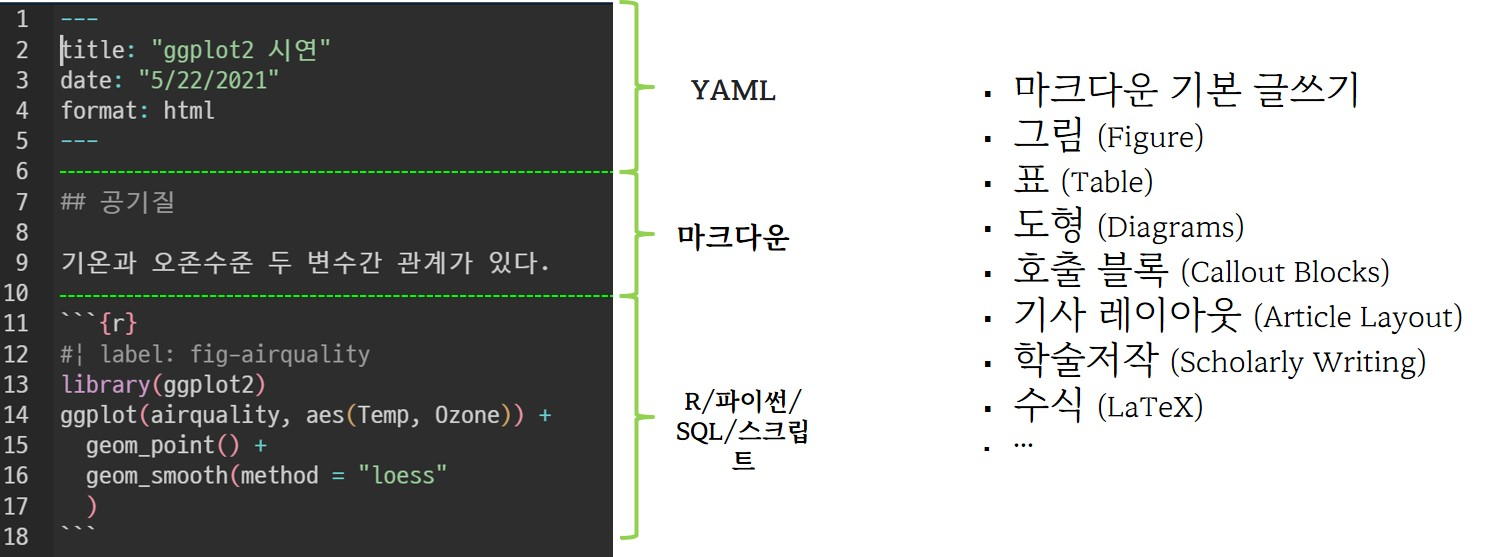
\includegraphics{images/layout_format.jpg}

}

\caption{문서 구조와 문학적 프로그래밍 (쿼토)}

\end{figure}

표, 그래프는 문서 구조와 문학적 프로그래밍의 중요성을 시각적으로
전달하는 중요한 매체다. R 언어 \texttt{tidyverse},
\texttt{palmerpenguins}, \texttt{gt} 패키지를 활용해 펭귄 데이터를
처리하고, 펭귄 종별 암수 개체수를 표로 정리하고 '펭귄종별 암수
개체수'라는 제목과 함께 데이터 출처를 표기하는 각주까지 표에 꼼꼼히
표기했다. 그래프 예시는 R 언어 \texttt{ggplot2} 패키지를 사용해 펭귄
물갈퀴 길이와 체질량 사이의 관계를 그래프로 표현하고 있다. 향후 표와
그래프는 영화 시놉시스 저작물의 중요한 문서 구성요소 중 하나로 활용될
것이다.

\begin{figure}

\begin{minipage}[t]{0.50\linewidth}

{\centering 

\hypertarget{uxd45c}{%
\subsection*{표}\label{uxd45c}}
\addcontentsline{toc}{subsection}{표}

\setlength{\LTpost}{0mm}
\begin{longtable*}{ccc}
\caption*{
{\large 펭귄종별 암수 개체수\textsuperscript{\textit{1}}}
} \\ 
\toprule
펭귄종 & 암컷 & 수컷 \\ 
\midrule
Adelie & 73 & 73 \\ 
Chinstrap & 34 & 34 \\ 
Gentoo & 58 & 61 \\ 
\bottomrule
\end{longtable*}
\begin{minipage}{\linewidth}
\textsuperscript{\textit{1}}데이터 출처: palmerpenguins 패키지\\
\end{minipage}

}

\end{minipage}%
%
\begin{minipage}[t]{0.50\linewidth}

{\centering 

\hypertarget{uxadf8uxb798uxd504}{%
\subsection*{그래프}\label{uxadf8uxb798uxd504}}
\addcontentsline{toc}{subsection}{그래프}

}

\end{minipage}%
\newline
\begin{minipage}[t]{0.50\linewidth}

{\centering 

\raisebox{-\height}{

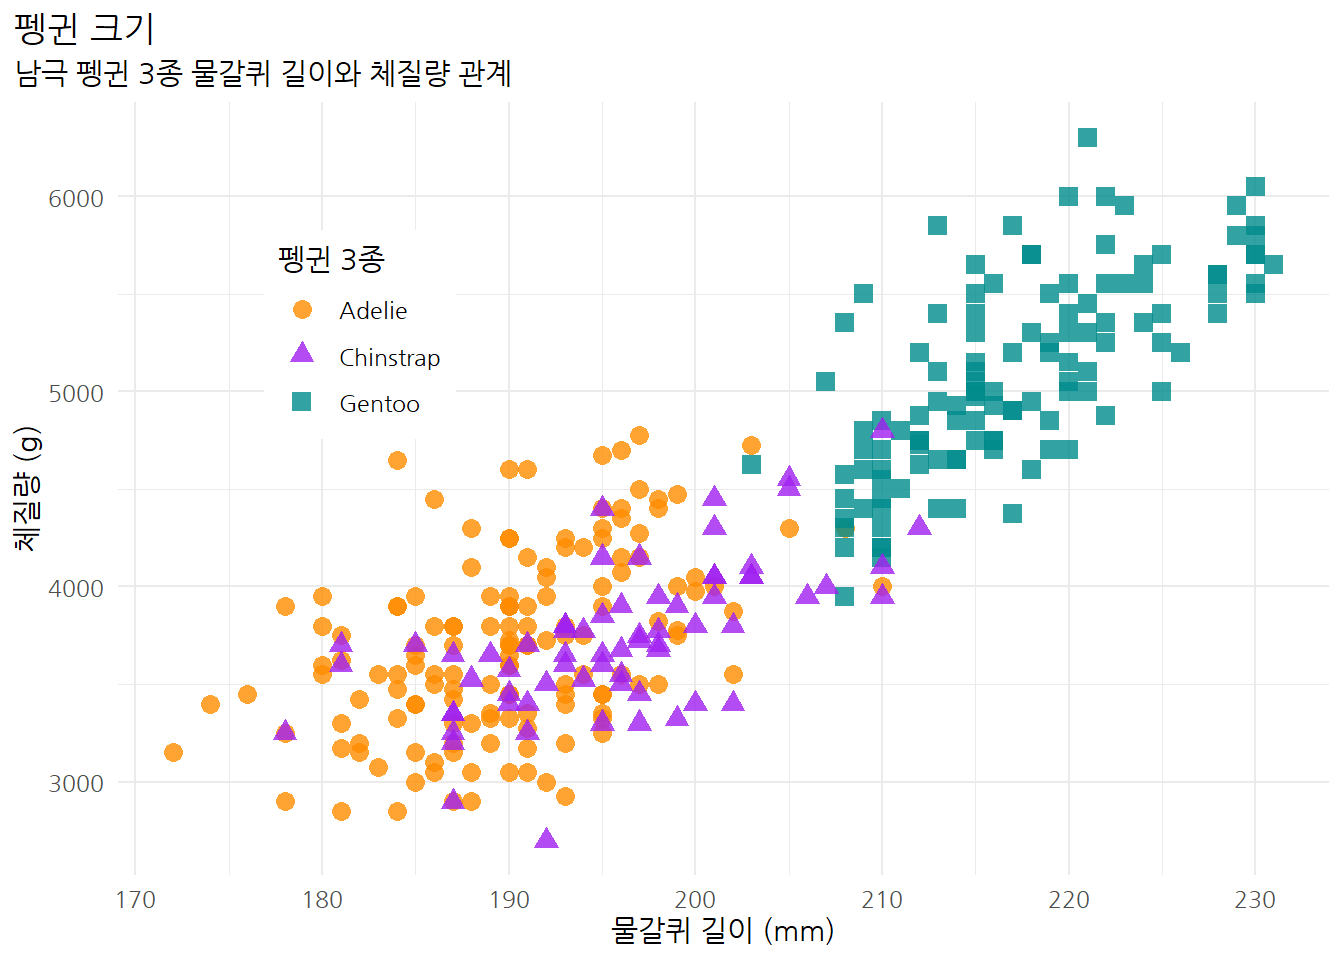
\includegraphics{images/whole_game_penguins.png}

}

}

\end{minipage}%

\end{figure}

\hypertarget{uxbc30uxd3ecuxc640-uxacf5uxc720}{%
\subsection{배포와 공유}\label{uxbc30uxd3ecuxc640-uxacf5uxc720}}

디지털 글쓰기 저작물을 완성한 후 다음 단계로 인쇄출판과 배포를 고려해야
한다. 과거와 달리 현재는 물론 앞으로 다양한 문서 저작물을 하나의
프로젝트로 엮어 전자출판을 할 수 있는 플랫폼이 필요하다.
\href{https://quartopub.com/}{\texttt{Quarto\ Pub}}은 이러한 목적으로
개발되어 저자가 작성한 다양한 문서저작물을 원클릭으로 전자출판할 수
있다. 물론 \href{https://quartopub.com/}{\texttt{Quarto\ Pub}} 외에도
\href{https://netlify.com/}{netlify}, \href{https://github.com/}{GitHub
Pages}, \href{https://www.rstudio.com/products/connect/}{RStudio
Connect} 등 다른 출판배포 플랫폼도 존재한다. 플랫폼들은 각각의 특성과
장점을 가지고 있어, 저자의 필요와 목적에 따라 적절한 플랫폼을 선택하여
디지털 글쓰기 저작물을 더 넓은 독자에게 전달할 수 있다.

최종 출판저작물 인쇄출판과 배포를 마친 후에는 저작물 공유도 고려할 수
있다. 저작물을 공유함으로써 저자는 자신의 저작물을 다른 사람들과
공유하고, 다른 사람들은 저작물을 활용할 수 있다. 저작물을 공유하는
방법은 다양하지만, 가장 쉬운 방법은 저작물을 공유할 수 있는 플랫폼에
저작물을 공유 저작권 표기를 함께 게시하는 것이다. 소스코드를 공유하면
다른 사람들이 문서 작성에 사용된 소스코드를 쉽게 이해하고, 문서 작성에
사용된 소스코드를 활용해 자신만의 향상된 저작물을 공유함으로써 글쓰기
문화를 확산시킬 수 있다.

\begin{figure}[H]

{\centering \includegraphics[width=9.16in,height=3.88in]{whole_game_files/figure-latex/mermaid-figure-2.png}

}

\end{figure}

챗GPT 디지털 글쓰기를 통해 저작한 문서는 다양한 형태로 배포될 수 있다.
``국제시장과 남극 펭귄''을 모티브로 삼아 제작한 다양한 영화 시놉시스
저작물은 다음과 같이 공개되어 있다.

\begin{itemize}
\tightlist
\item
  \href{https://statkclee.quarto.pub/writing-penguin/01_movie.html}{HTML
  웹페이지}: HTML 웹페이지 형식으로는 누구나 쉽게 접근하고 읽을 수
  있으며, 웹 브라우저만 있으면 어디서든 열람이 가능하다.
\item
  \href{https://statkclee.quarto.pub/writing-penguin/02_movie_pdf.pdf}{PDF
  파일}: PDF 파일 형식으로는 공식 문서나 보고서로 사용할 수 있으며,
  물리적인 출력이 필요할 때도 유용하다.
\item
  \href{https://statkclee.quarto.pub/writing-penguin/03_movie_ppt.html\#/title-slide}{PPT
  슬라이드}: PPT 슬라이드 형식으로는 발표나 강의 자료로 활용할 수 있어,
  다양한 상황에서 유연하게 사용할 수 있다.
\end{itemize}

문서 저작을 넘어 다양한 형식으로 문서를 배포하면, 독자나 이용자가
자신에게 가장 편리한 방식으로 문서를 열람할 수 있다. 따라서 챗GPT 디지털
글쓰기는 단순히 텍스트를 생성하는 것을 넘어, 다양한 배포 채널과 형식을
통해 더 넓은 독자층에게 접근할 수 있는 장점도 크다.

\begin{figure}

{\centering 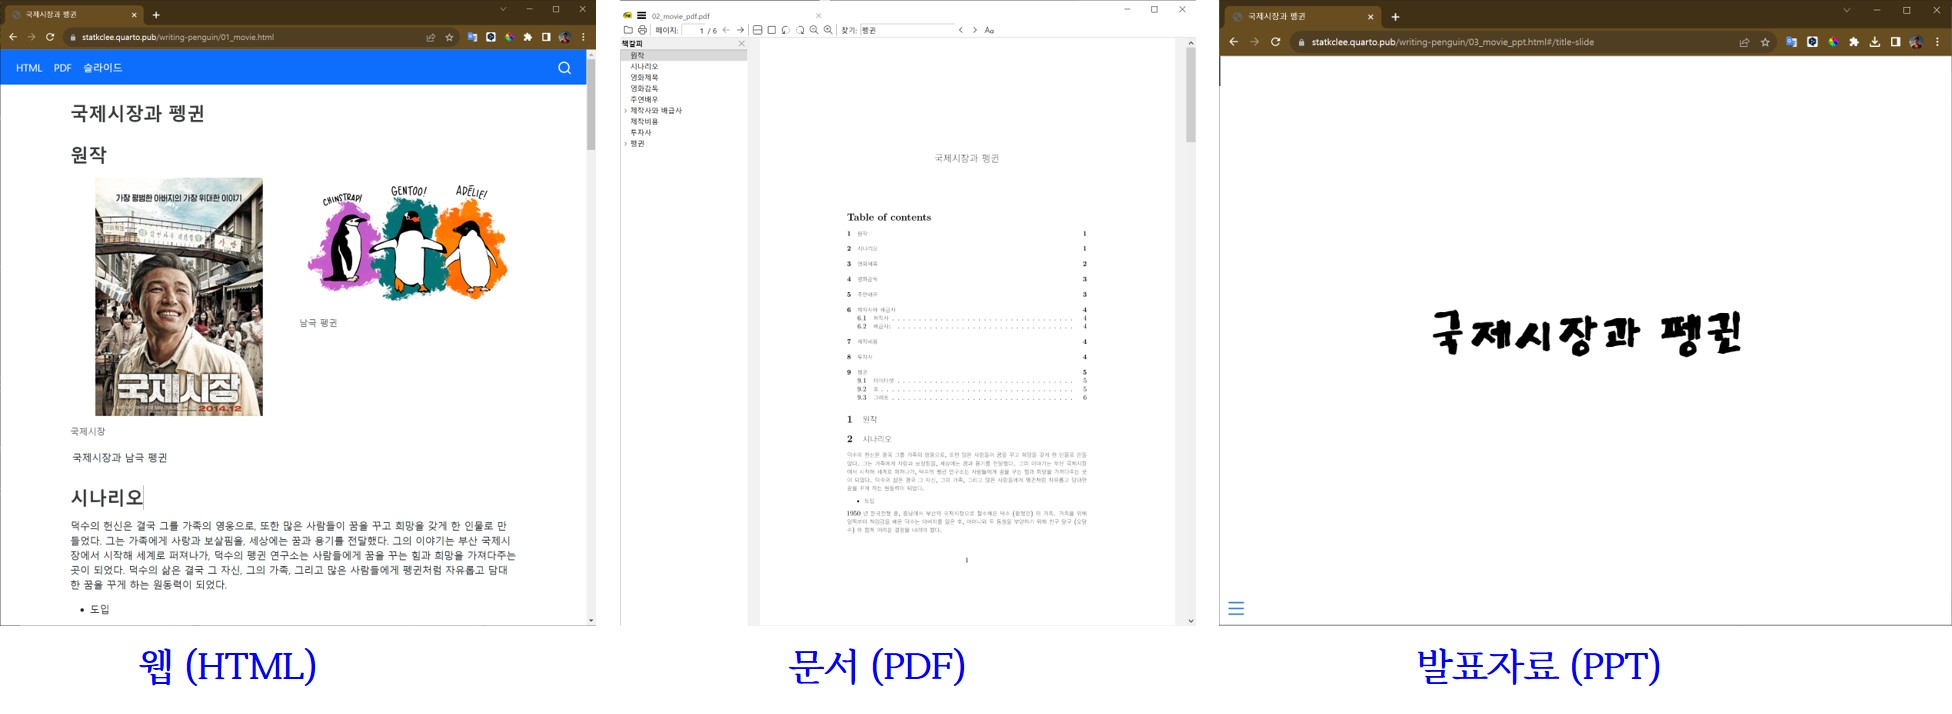
\includegraphics{images/chatGPT_quarto_deploy.jpg}

}

\caption{웹, 문서, PPT 슬라이드 배포}

\end{figure}

\part{글쓰기 환경}

\hypertarget{uxc5b8uxc5b4uxc640-uxbb38uxc790}{%
\chapter{언어와 문자}\label{uxc5b8uxc5b4uxc640-uxbb38uxc790}}

글쓰기 역사는 인류 문명과 밀접하게 연결되어 있다. 언어의 발전과 말하기가
수만 년 동안 이루어진 후에, 비로소 문자가 등장했다. 초기 문자 증거는 약
3000 BC경에 이집트와 메소포타미아에서 발견되었고, 중국에서도 거의
동시기에 독립적으로 발명되었다. 초창기 문자는 주로 상거래나 종교적 행사,
법률 등을 기록하기 위해 사용되었다.

특히 주목할 만한 점은 문자가 등장하기 전에 숫자가 먼저 다양한 형태로
사용되기 시작했다는 점이다. 초기 인류의 생존과 밀접한 관련이 있는
농업분야에서 경작지 면적, 수확량 계산, 별자리나 계절의 변화를 기록하여
더 많은 곡식을 얻기 위한 필요성 때문으로 보인다.

문자는 시간이 흐르면서 단순한 정보의 기록에서 벗어나, 다양한 목적과
사회적 문제 해결을 위한 중요한 도구로 진화해 왔다. 예를 들어, 고대
로마나 그리스에서는 법률과 철학, 역사 등을 글로 기록하였고, 이는 후대에
큰 영향을 미쳤다. 또한, 글쓰기는 문화와 예술, 심지어는 정치와 사회
변혁에도 중요한 역할을 하게 되었다.

\hypertarget{uxbb38uxc790-uxad6cuxc131uxc694uxc18c}{%
\section{문자 구성요소}\label{uxbb38uxc790-uxad6cuxc131uxc694uxc18c}}

의사소통과 정보 표현과 전달에 있어 중요한 차이를 가지는 언어(Language)와
문자(Writing System)를 구분하는 것은 중요하다. 언어는 음성, 제스처, 기호
등 다양한 형태로 표현되며, 문법, 어휘, 발음 등을 통해 의미를 전달한다.
이와 달리 문자는 언어를 시각적으로 표현하기 위한 기호체계로, 알파벳,
음절 문자, 로고그램 등 다양한 형태를 가진다. 언어는 문자 없이도 존재할
수 있으나, 문자는 특정 언어를 표현하고 기록하기 위해 존재한다.

문자가 존재하고 효과적으로 기능하기 위해서는 몇 가지 기본 조건이
필요하다. 언어, 생각, 기호, 매체가 문자가 존재하기 위해 필요한 조건이다.

\begin{itemize}
\item
  언어: 문자는 특정 언어(한국어, 영어, 중국어 등)의 표현 수단이다.
  언어의 복잡성과 다양성을 효과적으로 표현할 수 있는 체계적 문자 체계가
  필요하다.
\item
  생각: 문자는 복잡한 아이디어와 추상적인 개념, 감정 또는 전문 용어를
  표현하는데 사용된다. 문자는 아이디어를 구체화하고 전달하는데 필수적인
  수단이다.
\item
  기호: 문자 외에도 숫자, 수식, 교통표지, 음표, 화학식, 프로그래밍 구문
  등 다양한 기호와 표식을 사용하여 특정 정보나 의미를 전달한다.

  \begin{itemize}
  \tightlist
  \item
    언어 기호: 알파벳, 한글, 한자 등
  \item
    숫자와 수식: 수학적 표현, 공식 등
  \item
    교통표지 및 표식: 안전 지시, 경고 표시 등
  \end{itemize}
\item
  매체: 글쓰기를 기록하고 전송하는 물리적 또는 디지털 매체가 필요하다.
  종이와 파피루스와 같은 전통적인 매체에서 현재는 컴퓨터 디스플레이,
  SSD, 클라우드 디지털 저장소가 그 역할을 대신하고 있다.
\end{itemize}

언어와 문자를 모두 다루는 것은 지면관계상 불가능하여 한국어를 중심으로
문자에 대해 다루고, 아이디어와 개념에서는 전문 용어를 중심으로 한
과학기술 문서 저작, 기호와 표식에서는 한글을 중심으로 한 언어적 기호와
숫자와 수학적 기호, 마지막으로 매체에서는 PDF 종이출판과 웹 디지털출판을
중심으로 살펴본다.

\begin{figure}[H]

{\centering \includegraphics[width=22.07in,height=3.23in]{history_files/figure-latex/mermaid-figure-1.png}

}

\end{figure}

\hypertarget{uxc5b8uxc5b4uxc640-uxbb38uxc790-1}{%
\subsection{언어와 문자}\label{uxc5b8uxc5b4uxc640-uxbb38uxc790-1}}

위키백과 따르면 전세계 인구는 약 80억명(2030년 기준)에 이르며,
화자들에게 본토어로 성경을 제공할 목적으로 기독교 언어학 봉사단체
에스놀로그 통계에 따르면 7,168개(2023년 기준) 언어가 사용되고 있다. 이
중에서도 영어, 중국어, 힌디어, 스페인어, 프랑스어, 아랍어, 벵골어,
러시아어, 포르투갈어, 인도네시아어가 가장 많은 사용자를 보유하고 있다.
\footnote{자료출처:
  https://en.wikipedia.org/wiki/List\_of\_languages\_by\_total\_number\_of\_speakers}

\begin{longtable*}{clccc}
\toprule
 &  & \multicolumn{2}{c}{구분} &  \\ 
\cmidrule(lr){3-4}
순위 & 언어 & 모국어 & 제2언어 & 전체 \\ 
\midrule
1 & English & $380,000,000$ & $1,077,000,000$ & $1,456,000,000$ \\ 
2 & Mandarin Chinese & $939,000,000$ & $199,000,000$ & $1,138,000,000$ \\ 
3 & Hindi & $345,000,000$ & $266,000,000$ & $609,000,000$ \\ 
4 & Spanish & $485,000,000$ & $74,000,000$ & $559,000,000$ \\ 
5 & French & $81,000,000$ & $229,000,000$ & $310,000,000$ \\ 
6 & Modern Standard Arabic & $0$ & $274,000,000$ & $274,000,000$ \\ 
7 & Bengali & $234,000,000$ & $39,000,000$ & $273,000,000$ \\ 
8 & Portuguese & $236,000,000$ & $27,000,000$ & $264,000,000$ \\ 
9 & Russian & $147,000,000$ & $108,000,000$ & $255,000,000$ \\ 
10 & Urdu & $71,000,000$ & $161,000,000$ & $232,000,000$ \\ 
13 & Japanese & $123,000,000$ & $200,000$ & $123,000,000$ \\ 
21 & Vietnamese & $85,000,000$ & $1,000,000$ & $86,000,000$ \\ 
24 & Korean & $82,000,000$ & $29,000,000,000$ & $82,000,000$ \\ 
29 & Italian & $65,000,000$ & $3,000,000$ & $68,000,000$ \\ 
\bottomrule
\end{longtable*}

전세계에는 7,000개가 넘는 언어가 존재하나, 이를 표현하는 문자 체계는
대략 50개 정도에 불과하다. 한국어(제주어 포함)는 한글을 문자 체계로
사용하고 있지만, 이처럼 모든 언어가 고유의 \textbf{문자(Writing
System)}를 가진 것은 아니다. 실제로 여러 언어가 동일한 문자 체계를
공유하는 경우가 많다. 예를 들어, 알파벳은 라틴어를 기반으로 하며, 영어,
불어, 독어, 이태리어 등 다양한 언어에서 사용되고 있다. 이 외에도 셀틱어,
발틱어, 슬로박어 등도 알파벳이 활용된다. 한자는 중국어와 대만어에서 주로
사용되며, 아랍문자는 아랍어뿐만 아니라 인도-이란 어족(페르시아어, 펀잡어
등)에도 쓰인다. 일본어는 가나(仮名)라는 문자 체계가 사용된다.

\begin{longtable*}{llc}
\toprule
스크립트\_명칭 & 문자유형 & 인구수 \\ 
\midrule
Latin Latin & Alphabet & $4,900,000,000$ \\ 
Chinese 汉字 漢字 & Logographic & $1,541,000,000$ \\ 
Arabic العربية & Abjad or Abugida (when diacritics are used) & $828,000,000$ \\ 
Devanagari देवनागरी & Abugida & $480,500,000$ \\ 
Cyrillic Кирилица & Alphabet & $289,000,000$ \\ 
Bengali–Assamese বাংলা-অসমীয়া & Abugida & $234,000,000$ \\ 
Kana かな カナ & Syllabary & $123,000,000$ \\ 
Telugu తెలుగు & Abugida & $83,000,000$ \\ 
Hangul 한글 조선글 & Alphabet, featural & $81,700,000$ \\ 
Tamil தமிழ் & Abugida & $78,600,000$ \\ 
\bottomrule
\end{longtable*}

\hypertarget{uxb9e4uxccb4uxc758-uxc5eduxc0ac}{%
\subsection{매체의 역사}\label{uxb9e4uxccb4uxc758-uxc5eduxc0ac}}

글쓰기와 문자의 발전은 인류 역사와 밀접하게 연결되어 있다. 초기에는
상형문자와 같은 시각적 기호를 사용하여 의미를 전달했으며 기원전
16,500년에 라스코 동굴벽화와 반구암각화 등에서 볼 수 있듯이 동굴벽면이나
돌 등을 매체로 사용했다.

수메르 문명의 출현과 함께 사람들이 집단으로 생활하기 시작하면서 도시화가
급속히 진행되었다. 이로 인해 세금 징수, 계약, 무역 등 복잡한 사회적,
정치적, 경제적 문제가 발생했고, 이를 해결하기 위해 더욱 정교한 문자
체계가 필요하게 되었다. 수메르에서는 다양한 정보를 기록하고 보존할 수
있도록 점토를 매체로 사용였다.

이집트 문명도 유사한 문제에 봉착했으며 매체로 점토 대신 파피루스를
사용했다. 파피루스는 더 가볍고 휴대하기 쉬워 글쓰기와 정보 보존 및
전달이 더욱 효율적으로 이루어졌다.

\begin{figure}

{\centering 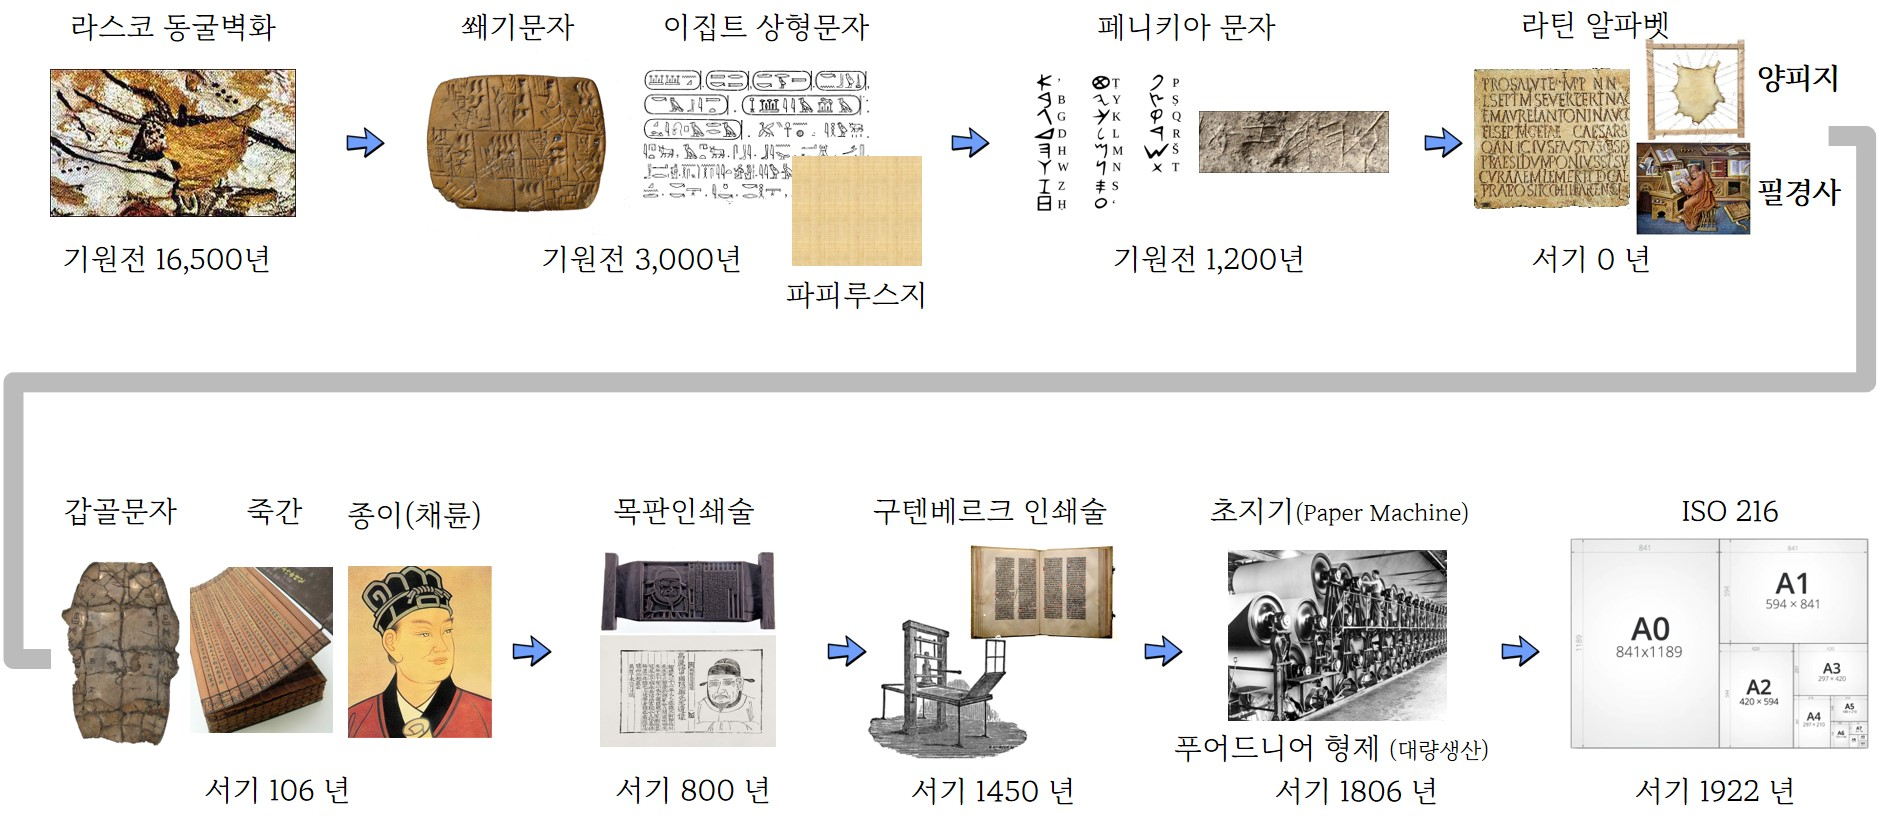
\includegraphics{images/writing-history.jpg}

}

\caption{문자 매체의 진화}

\end{figure}

문자를 담을 수 있는 매체로 초기에는 동굴벽이나 돌, 점토 등을 사용했지만,
이러한 매체는 비용이 많이 들고 유지관리가 어려웠다. 또한 상형문자가 담을
수 있는 정보에 한계가 있어, 더 효율적인 방법이 필요했다.

먼저 서양에서는 페니키아인들이 이러한 문제를 해결하기 위해 기원전
1,200년에 페니키아 문자를 창안했다. 이 문자는 소리에 의미를 담을 수
있어, 상형문제에 비해 무한대에 가까운 의미를 표현할 수 있고 같은 지중해
문명권 그리스와 로마 문화를 거쳐 라틴 알파벳이 공표되었고, 이를 담을 수
있는 매체로 양피지가 채택되었다.

한편 중국에서는 106년에는 채륜이 종이를 발명함으로써 글쓰기 문화에 큰
변화가 일어났다. 서기 800년경 목판인쇄술이, 1450년 구텐베르크 인쇄술이
발명되어 출판의 대량 생산이 가능해졌다. 1806년에는 푸어드니어 형제가
종이를 대량으로 생산할 수 있는 초지기를 발명, 저렴한 비용으로 일반
대중도 생각을 문자로 기록하고 널리 자신의 생각을 알릴 수 있게 되었다.
1922년 ISO 216을 통해 종이에 대한 국제 표준이 확립되어 미국을 제외한
대부분의 국가에서는 문자를 담을 수 있는 종이 매체에 대한 표준이
확립되었다.

\hypertarget{uxbb38uxc790}{%
\subsection{문자}\label{uxbb38uxc790}}

언어를 기록하기 위한 상징체계로 \textbf{문자(文字, writing system)}가
발명되었다. 문자는 언어 중에서도 음성언어를 기록하기 위해 생겨난 것으로
알려져 있다. 문자의 중요성은 정보의 저장과 전달에 있어 신뢰성이 담보되기
때문에 크다. 문자는 크게 두 가지 유형으로 분류된다.

\begin{enumerate}
\def\labelenumi{\arabic{enumi}.}
\item
  \textbf{표의문자(Logographic)}: 그림이나 상징을 사용하여 단어나 개념을
  직접 나타낸다. 중국 한문과 이집트 상형문자가 대표적으로, '木'은
  '목'이라는 소리를 내지만, 그 뜻은 '나무'다.
\item
  \textbf{표음문자(Phonographic)}: 발음이나 소리를 나타내기 위해
  설계되었고, 한글, 라틴 알파벳 등 대부분의 언어가 이 유형에 속한다.
\end{enumerate}

\begin{figure}

{\centering 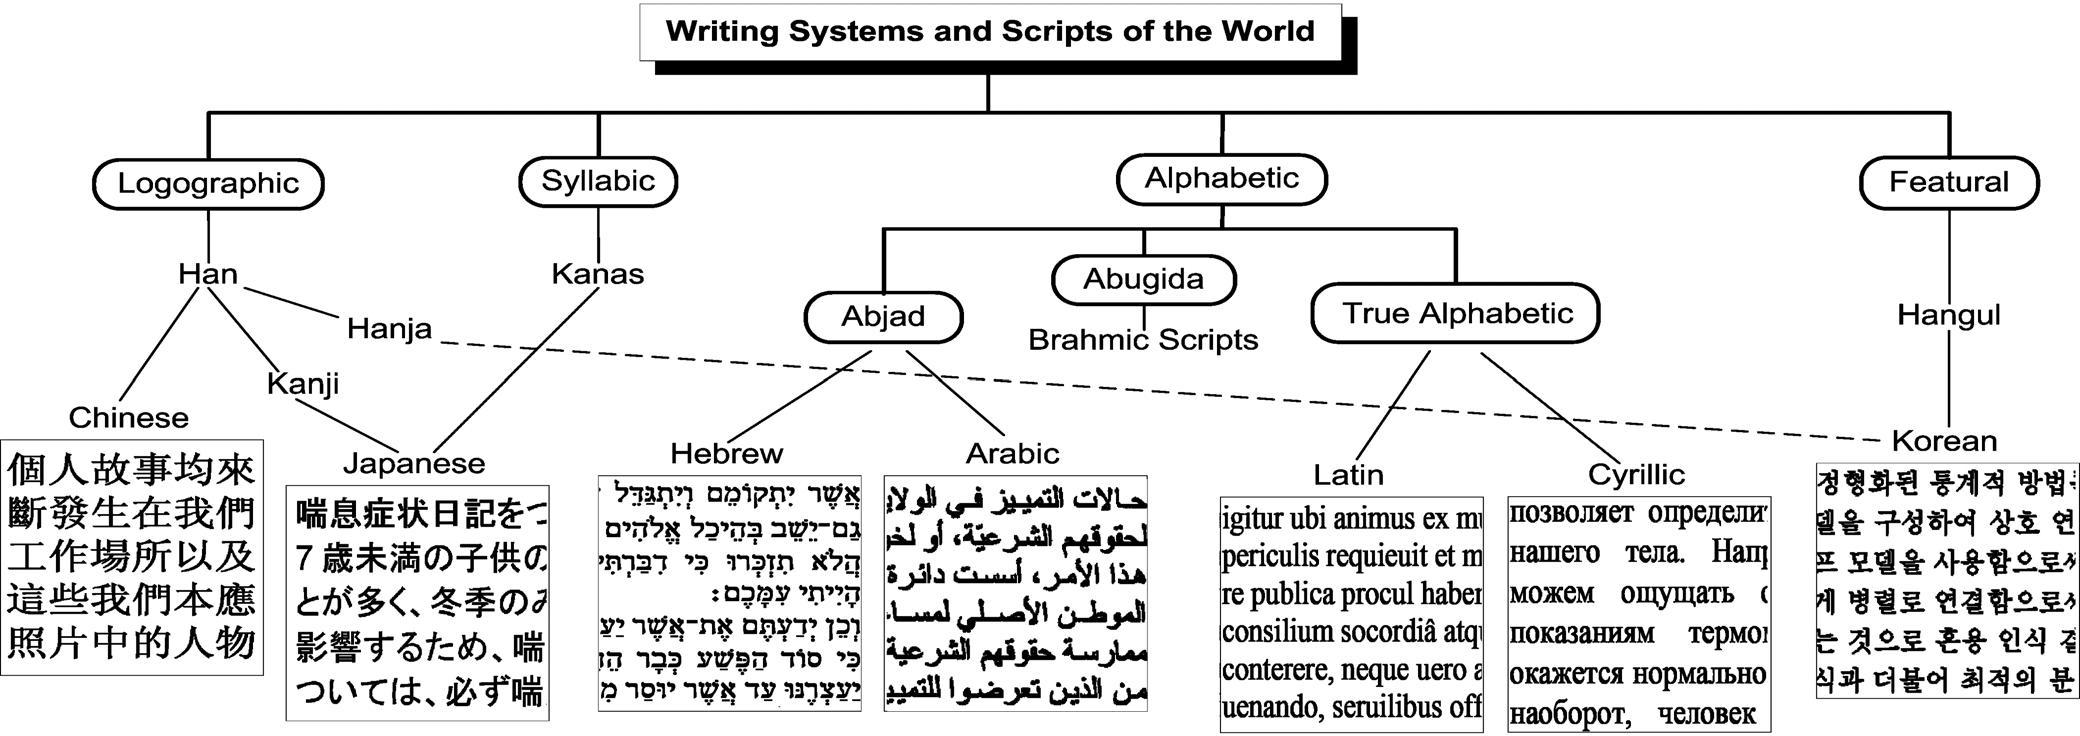
\includegraphics{images/writing-systems.png}

}

\caption{문자와 스크립트}

\end{figure}

표의문자는 상징이나 그림을 통해 의미를 전달하므로, 하나의 문자가 복잡한
개념이나 단어를 나타낼 수 있는 반면에 표음문자는 소리를 기반으로 하므로,
단순하고 규칙적인 구조를 가지며, 다양한 단어와 문장을 구성하기에
유용하다. 표의문자는 의미를 전달하기 위해 그림이나 상징을 사용하므로,
그림이나 상징을 알지 못하면 의미를 전달할 수 없기 때문에 문자 수가
많아지고, 학습에 많은 시간이 필요하다. 반면에 표음문자는 소리를 기반으로
하므로, 문자를 조합하여 의미를 만들기 때문에 문자 수가 적고, 학습에
상대적으로 적은 시간이 필요하다.

\begin{longtable}[]{@{}
  >{\centering\arraybackslash}p{(\columnwidth - 6\tabcolsep) * \real{0.2027}}
  >{\centering\arraybackslash}p{(\columnwidth - 6\tabcolsep) * \real{0.2027}}
  >{\centering\arraybackslash}p{(\columnwidth - 6\tabcolsep) * \real{0.2027}}
  >{\centering\arraybackslash}p{(\columnwidth - 6\tabcolsep) * \real{0.3919}}@{}}
\toprule\noalign{}
\begin{minipage}[b]{\linewidth}\centering
문자체계
\end{minipage} & \begin{minipage}[b]{\linewidth}\centering
문자 수
\end{minipage} & \begin{minipage}[b]{\linewidth}\centering
문자 구분
\end{minipage} & \begin{minipage}[b]{\linewidth}\centering
설명
\end{minipage} \\
\midrule\noalign{}
\endhead
\bottomrule\noalign{}
\endlastfoot
라틴 알파벳 & 26 & 알파벳 & 영어와 다른 라틴계 언어 사용 \\
한글 & 14 자음, 10 모음 & 자음, 모음 & 한국어 사용 \\
중국어 한자 & 50,000+ & 한자 & 중국어 사용되며, 일부는 일본어, 한국어
사용 \\
아랍 알파벳 & 28 & 알파벳 & 아랍어와 다른 인도-이란 어족 언어 사용 \\
히브리 알파벳 & 22 & 알파벳 & 히브리어 사용 \\
키릴 알파벳 & 33 & 알파벳 & 러시아어와 다른 슬라브 언어 사용 \\
데바나가리 & 47\textasciitilde52 & 알파벳 & 힌디어와 다른 인도 언어
사용 \\
그리스 알파벳 & 24 & 알파벳 & 그리스어 사용 \\
일본어 가나 & 46 가타카나, 46 히라가나 & 가타카나, 히라가나 & 일본어
사용 \\
\end{longtable}

\begin{tcolorbox}[enhanced jigsaw, opacityback=0, opacitybacktitle=0.6, colback=white, rightrule=.15mm, coltitle=black, colframe=quarto-callout-note-color-frame, colbacktitle=quarto-callout-note-color!10!white, bottomrule=.15mm, bottomtitle=1mm, breakable, title=\textcolor{quarto-callout-note-color}{\faInfo}\hspace{0.5em}{문자와 스크립트}, titlerule=0mm, leftrule=.75mm, toptitle=1mm, left=2mm, arc=.35mm, toprule=.15mm]

문자는 \textbf{`무엇(what)'}을 기록할 것인지에 대한 체계나 원칙이며,
스크립트는 \textbf{`어떻게(how)'} 그것을 기록할 것인지에 대한 구체적인
방법으로 나눠볼 수 있다.

\begin{itemize}
\item
  문자(Wriring System): 언어를 기록하기 위한 전반적인 방법론이나 체계를
  의미하며, 언어의 특정 부분(예: 음성, 의미, 문법 등)을 어떻게 표현할
  것인지에 대한 규칙과 원칙이 포함된다. 문자는 언어의 복잡성과 뉘앙스를
  어떻게 효과적으로 포착할 것인지에 대한 방법을 제공한다. 예를 들어,
  알파벳, 로고그램, 음절 문자 등을 들 수 있다.
\item
  스크립트(Scripts): 특정 글쓰기 시스템을 구현하는 데 사용되는 문자
  집합을 의미한다. 스크립트는 문자의 '글꼴(폰트)'이나 '스타일'과 같은
  것으로 생각할 수 있다. 예를 들어, 라틴 스크립트, 한글, 한자 등을 들 수
  있다.
\end{itemize}

\end{tcolorbox}

앞서 문자를 크게 표음문자와 표의문자로 구분하였다. 이를 좀더 상세히
세분화하면 전세계 문자는 크게 다음과 같이 4개로 구분된다. 첫 번째는
표어문자(Logographic)로, 하나의 문자는 하나의 단어나 개념을 나타낸다.
대표적으로 중국의 한자가 있으며, 예를 들어 `木' 문자는 `나무'라는 개념을
나타낸다. 두 번째는 음절문자(Syllabic)로, 하나의 문자가 하나의 음절을
나타낸다. 일본어의 가나(ひらがな, カタカナ)가 이에 해당하며, 'か' 문자는
`ka'라는 음절을 나타낸다. 세 번째는 음소문자(Alphabetic)로, 하나의
문자가 하나의 음소(최소 음성 단위)를 나타낸다. 로마자로 대표되는
영문자가 이에 해당하며, 'A' 문자는 `에이'라는 음소를 나타낸다.
마지막으로 자질문자(Featural)로 문자의 형태가 그 문자가 나타내는
발음이나 음성 자질과 직접적으로 관련이 있다. 한글이 대표적인 예로, 'ㄱ'
문자는 뒷니와 혀가 만나는 위치에서 나는 소리를 나타낸다.
\autocite{gohos2010}

\begin{longtable}[]{@{}ccc@{}}
\toprule\noalign{}
\textbf{종류} & \textbf{기호 표현} & \textbf{예} \\
\midrule\noalign{}
\endhead
\bottomrule\noalign{}
\endlastfoot
표어 문자 & 형태소 & 중국 한자 \\
음절 문자 & 음절 또는 모라 & 일본 가나 (문자) \\
음소 문자 & 낱소리 (자음 또는 모음) & 로마자, 키릴문자, 그리스 문자 \\
아부기다 & 낱소리 (자음+모음) & 데바나가리 문자, 그으즈 문자 \\
아브자드 & 낱소리 (자음) & 아랍 문자, 히브리 문자 \\
자질 문자 & 음성 자질 & 한국 한글 \\
\end{longtable}

\hypertarget{uxc54cuxd30cuxbcb3}{%
\subsubsection{알파벳}\label{uxc54cuxd30cuxbcb3}}

알파벳(Alphabet) 역사는 매우 흥미롭다. 이집트 상형문자에서 시작하여
페니키아 상인을 거쳐 그리스와 로마로 이어지는 과정은 언어와 문자의
진화를 잘 보여준다. 특히, 페니키아 상인이 소리를 기반으로 의미를
전달하는 방식을 채택한 것은 문자의 역사에서 중요한 전환점이다. 이전에는
이집트 상형문자와 같은 표의문자가 주로 사용되었는데, 이러한 문자는
그림이나 상징을 통해 의미를 전달하는 방식은 복잡하고 비효율적이었다.
특히 상업적인 거래나 다양한 문화와 언어 간의 소통에서는 이러한 복잡성이
큰 장애였다.

페니키아 상인들은 문제를 해결하기 위해 소리를 기반으로 한 새로운 문자
체계를 도입했다. 각 문자의 특정 소리나 발음을 조합하여 단순하고 효율적인
의사소통이 가능하게 된다. 표음문자 도입은 상업적인 거래를 더욱 원활하게
하고, 다양한 언어와 문화 간의 소통을 쉽게 만들었으며 알파벳 문자 체계로
발전할 수 있는 기반을 마련했다. 그리스에서 알파벳 뒤쪽 문자가 추가되고,
로마시대에 비로소 오늘날 알려진 영어 대문자가 완성되었다. 이후 소문자는
손으로 필사하는 과정에서 발명되었고, 다양한 글꼴도 생겨났다. 구텐베르그
활자인쇄술 발명은 현재와 같은 알파벳 문자 완성을 가능하게 했다.
\footnote{{[}Evolution of the Alphabet \textbar{} Earliest Forms to
  Modern Latin Script
  \href{https://www.youtube.com/watch?v=3kGuN8WIGNc}{유튜브}{]}}

\begin{figure}

{\centering 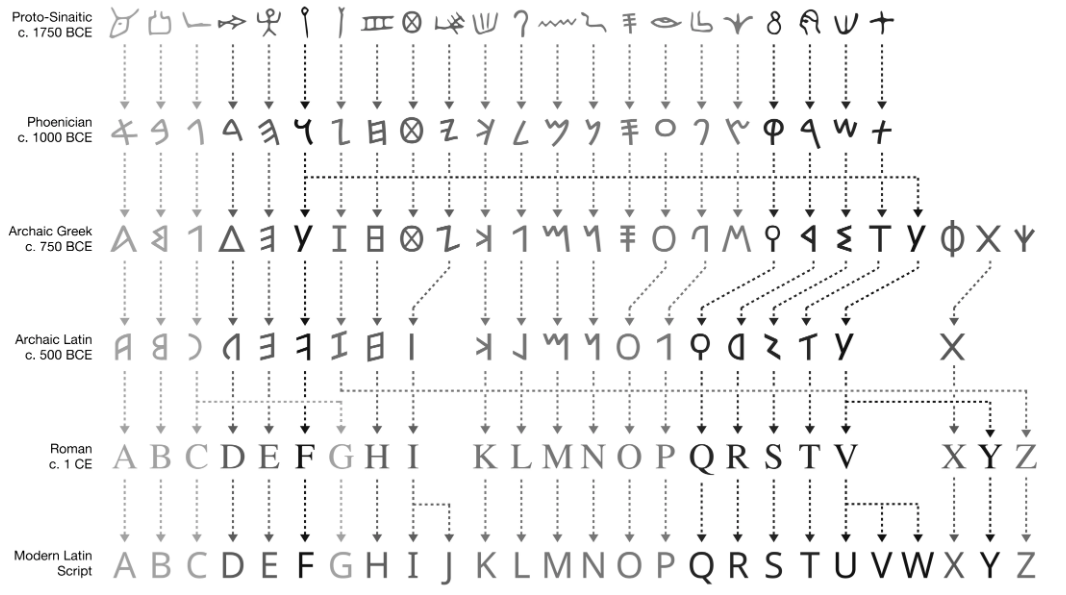
\includegraphics{images/writing-alphabet.png}

}

\caption{알파벳 문자 진화 역사}

\end{figure}

\begin{verbatim}
#> 알파벳 대문자:  26 개
#>  A B C D E F G H I J K L M N O P Q R S T U V W X Y Z
#> 알파벳 소문자:  26 개
#>  a b c d e f g h i j k l m n o p q r s t u v w x y z
\end{verbatim}

\hypertarget{uxd45cuxc758-uxbb38uxc790}{%
\subsubsection{표의 문자}\label{uxd45cuxc758-uxbb38uxc790}}

한자와 같은 표의 문자가 여러가지 단점이 있는 것처럼 보이기도 하지만
표의문자가 갖는 장점으로 인해 그 중요성이 더욱 부각되고 있다. 표의문자가
갖는 장점은 문자 자체 의미가 부여되기 때문에 전세계 누구도 문자만 보면
그 뜻을 유추할 수 있다는 점이다.

표의문자의 장점은 의미 자체가 문자에 내재되어 있기 때문에, 언어의 장벽을
뛰어넘을 수 있다. 예를 들어, 한자로 쓰인 '木'는 '나무'라는 의미를 가지고
있어 언어에 상관없이 일관된다. 따라서 중국어를 모르는 사람도 이 문자를
보고 '나무'라는 개념을 이해할 수 있다. 이러한 특성은 다양한 언어와
문화가 교차하는 글로벌한 환경에서 매우 유용하다. 표의문자는 복잡한
개념이나 아이디어를 간결하고 명확하게 전달할 수 있고 시각적인 요소가
강하기 때문에 디자인이나 예술 작업에도 자주 사용된다. 하지만, 의미가
복잡하거나 추상적인 경우, 하나의 문자로 그 의미를 완전히 표현하기 어렵고
표의문자를 익히고 제대로 사용하기 위해서 상대적으로 높은 학습 비용은
단점으로 꼽을 수 있다.

\begin{itemize}
\tightlist
\item
  그림문자(Pictographic): 😵, 🙋, 🍰, \ldots{}
\item
  표의문자(Ideogrpahic): 🚫 금지와 같은 의미를 갖는 문자로 ⛔ 🚸 교통
  표지판, ▶️ 전자제품 사용
\item
  추상 어표(Abstract Logograpahic): 한자 사람 인(人), \%, \&, \ldots{}
\end{itemize}

그림문자와 표의문자를 결합하면 매우 효과적인 의사소통 도구가 될 수 있다.
예를 들어, ``금연''이라는 표의문자와 금지를 나타내는 원형의 빨간색 선을
그림으로 표현한 그림문자를 함께 사용하면, 언어의 장벽 없이 ``흡연
금지''라는 메시지를 명확하게 전달할 수 있어, 공공장소, 국제공항, 다양한
문화 및 언어가 혼재된 환경에서 특히 유용하다. 단순한 텍스트나 단일한
그림만 사용하는 것보다 사람들이 다양한 언어와 문화 배경을 가지고 있을
때, 그림문자와 표의문자의 조합은 메시지를 빠르고 명확하게 전달하는 데 큰
도움을 준다.

\begin{figure}

{\centering 
\includegraphics{images/pictogram_ideogram.jpg}

}

\caption{흡연과 금지가 결합된 표의문자}

\end{figure}

\hypertarget{uxc790uxc9c8uxbb38uxc790-uxd55cuxae00}{%
\subsubsection{자질문자
(한글)}\label{uxc790uxc9c8uxbb38uxc790-uxd55cuxae00}}

자질문자(featural alphabet)는 문자가 그 문자가 표현하는 소리의
특징(자질)을 시각적으로 나타내는 문자 체계를 의미한다. 즉, 문자의 형태가
그 문자가 나타내는 발음이나 음성 자질과 직접적으로 관련있는 체계로
문자를 배우고 이해하기 쉽다.

자질문자의 대표적인 예로 한글이 꼽힌다. 한글 자음 문자는 발음하는
입모양을 나타내려고 설계되었고, 모음 문자는 혀의 위치와 움직임을
나타낸다. 자질문자는 발음의 물리적, 생리적 특성을 문자에 반영하기
때문에, 언어의 발음 체계에 변화가 생겨도 그에 따라 쉽게 수정이
가능하다는 장점이 있고, 이러한 설계 덕분에 한글은 상대적으로 배우기 쉽고
효율적인 문자 체계로 평가된다.

한글은 세종대왕에 의해 창제되어 한국어를 표기하기 위한 고유문자다.
표음문자와 자질문자의 특성을 모두 가지고 있어, 한자와 달리 음소를
정확하게 표현할 수 있다. 창제 초기에는 홀소리(모음) 11개와 닿소리(자음)
17개, 총 28개의 문자로 구성되었으나, 현재는 홀소리 10개와 닿소리 14개,
총 24개 기본 문자만 사용한다.

한글은 그 구조적 우수성과 표기의 정확성 때문에 지속적인 연구와 보급이
이루어졌고, 음소 단위 표기가 가능하여 매우 높은 표기 정확성을 자랑한다.
20세기에 들어, 다양한 학문 분야에서 한글 구조와 기능에 대한 연구가
활발히 이루어져, 한글만의 고유한 문법과 표기법이 정립되어, 현재 한국어
뿐만 아니라 제주어, 찌아찌아어 등 다양한 언어와 방언의 표기에도 널리
사용되고 있다.

\begin{verbatim}
#> 한글 자음:  14 개
#>  ㄱ ㄴ ㄷ ㄹ ㅁ ㅂ ㅅ ㅇ ㅈ ㅊ ㅋ ㅌ ㅍ ㅎ
#> 한글 모음:  10 개
#>  ㅏ ㅑ ㅓ ㅕ ㅗ ㅛ ㅜ ㅠ ㅡ ㅣ
\end{verbatim}

\hypertarget{uxae30uxd638uxc758-uxc5eduxc0ac}{%
\section{기호의 역사}\label{uxae30uxd638uxc758-uxc5eduxc0ac}}

문자는 사람의 필요와 유행에 항상 변화하고 발전했다. 초기에는
토큰(token)이라고 불리는 간단한 기호나 물체를 사용하여 정보를 저장하고
전달하는 목적으로 주로 물품 거래나 세금 징수 등을 기록하기 위해
사용되었다. 그 다음 단계로 그림문자(pictogram)가 등장했는데 상징적인
그림을 통해 단순한 정보나 개념을 표현하는 방식이었다.
로고그래피(logography)는 그림문자를 발전시킨 형태로, 특정 단어나 개념을
나타내는 문자를 사용한다는 점에서 시각중심에서 청각중심으로 전환을
의미했다. 알파벳은 로고그래피에서 더욱 발전하여, 언어소리를 분할하여
나타내는 문자로 언어의 복잡성을 더욱 정교하게 표현할 수 있도록 했다.
한글은 조선시대에 이르러 가장 늦게 발명되었는데, 기존 문자를 자체적으로
분석하고 이해하여 전혀 새롭고 효율적인 문자를 만들어낸 결과물이다.

\begin{itemize}
\item
  상형문자(기원전 6000\textasciitilde4000년경): 초기 문자 형태인
  픽토그래프(Pictograph)는 사물이나 아이디어를 나타내는 단순한 그림이나
  기호였다. 수메르, 이집트, 중국에서 기본적인 정보를 전달하기 위해
  사용되었다.
\item
  설형 문자(기원전 3400\textasciitilde3200년경): 고대 수메르(현대
  이라크)에서 개발된 설형문자는 초기 문자 체계 중 하나로 간주된다.
  상형문자에서 발전한 문자로 점토판에 쐐기 모양의 스타일러스를 눌러
  단어와 아이디어를 나타내는 일련의 쐐기 모양의 자국을 만들어 표현했다.
\item
  이집트 상형문자(기원전 3200\textasciitilde3000년경): 고대 이집트인들은
  음성 기호와 표의 문자를 조합하여 사용하는 이집트 상형문자를 개발했다.
  상형문자는 종교 텍스트, 비문, 공식 문서에 사용되었다.
\item
  페니키아 알파벳(기원전 1200년경): 페니키아 알파벳은 이집트
  상형문자에서 파생된 초기 알파벳 문자다. 각 기호가 고유한 소리를
  나타내는 알파벳 개념을 도입하여 문자 발전에 있어 중요한 발전을
  이루어냈다.
\item
  그리스 알파벳(기원전 800년경): 그리스 알파벳은 페니키아 알파벳에서
  발전하여 모음을 도입하여 문자 표현력을 크게 향상시켰으며, 그리스
  알파벳은 라틴어와 키릴 문자를 비롯한 많은 현대 유럽 문자 체계의 토대를
  마련했다.
\item
  라틴 알파벳(기원전 700년경): 고대 로마인들이 사용한 라틴 알파벳은
  그리스 알파벳에서 파생되었다. 시간이 지남에 따라 발전하여 영어,
  스페인어, 프랑스어, 독일어 등 많은 현대 문자의 기초를 형성하고 있다.
\item
  중국어 문자(기원전 1200년경): 중국어 문자(한자)는 상형문자에서
  발전하여 각 문자가 단어 또는 형태소(의미 단위)를 나타내는 복잡한
  로고그램으로 발전했다. 한자는 일본어와 한국어 등 다른 동아시아 문자
  체계의 발전에 영향을 미쳤다.
\item
  브라흐미 문자(기원전 300년경): 브라흐미 문자는 고대 인도에서
  개발되었으며 데바나가리(힌디어와 산스크리트어에 사용), 타밀어,
  태국어를 비롯한 많은 남아시아 및 동남아시아 문자의 조상으로 간주된다.
\item
  아랍 문자(기원전 4세기경): 나바테아 알파벳에서 발전한 아랍 문자는
  아랍어를 표기하는 데 사용되며 페르시아어, 우르두어, 파슈토어 등 다른
  언어와 함께 사용할 수 있도록 변형되었다.
\item
  키릴 문자(기원전 9세기경): 러시아어와 다른 여러 슬라브어를 표기하는 데
  사용되는 키릴 문자는 선교사 형제인 시릴과 메토디우스가 제1차 불가리아
  제국에서 개발했다. 그리스 알파벳을 기반으로 슬라브어 고유의 소리를
  표현하기 위한 문자가 추가되었다.
\item
  한글(기원후 14세기): 조선전기 제4대 세종대왕이 훈민정음이라는 이름으로
  창제하여 반포한 우리나라 고유의 문자다. 한글은 다른 나라의 기원과 발달
  과정에 비하면 전혀 다른 과정을 거쳐 온 문자로, 세종대왕을 중심으로 한
  소수의 집현전 학자들에 의해 치밀하게 계획되어 처음부터 완전한 글자꼴과
  표현 원리를 정해 1443년에 창제되어 세종28년 1446년에 10월에 반포한
  것으로 이러한 독창적인 글자를 만든 일은 세계 역사에 일찍이 찾아볼 수
  없다.
\end{itemize}

\hypertarget{uxd3b8uxc9d1uxae30uxc640-uxcd9cuxd310}{%
\chapter{편집기와 출판}\label{uxd3b8uxc9d1uxae30uxc640-uxcd9cuxd310}}

디지털 전환(Digital Transformation) 전 글쓰기는 착상 후 종이와 연필을
가지고 글을 작성하고 수차례 수정작업을 거쳐 타자기로 탈고를 하고 이를
출판사에 넘겨 책이나 보고서로 고객에게 전달하게 된다. 하지만,
\textbf{디지털 전환(Digital Transformation)} 시대 도래로 글쓰기 방식도
크게 변화하게 된다. 아래한글이나 마이크로소프트 워드, 리브레 Write와
같은 워드 프로세서(Word Processor)를 넘어, Vim, Emacs, VS 코드와 같은
코딩 편집기에서 마크다운을 사용하거나 직접 HTML을 코딩하여 글쓰기를 하게
된다.

\begin{figure}

{\centering 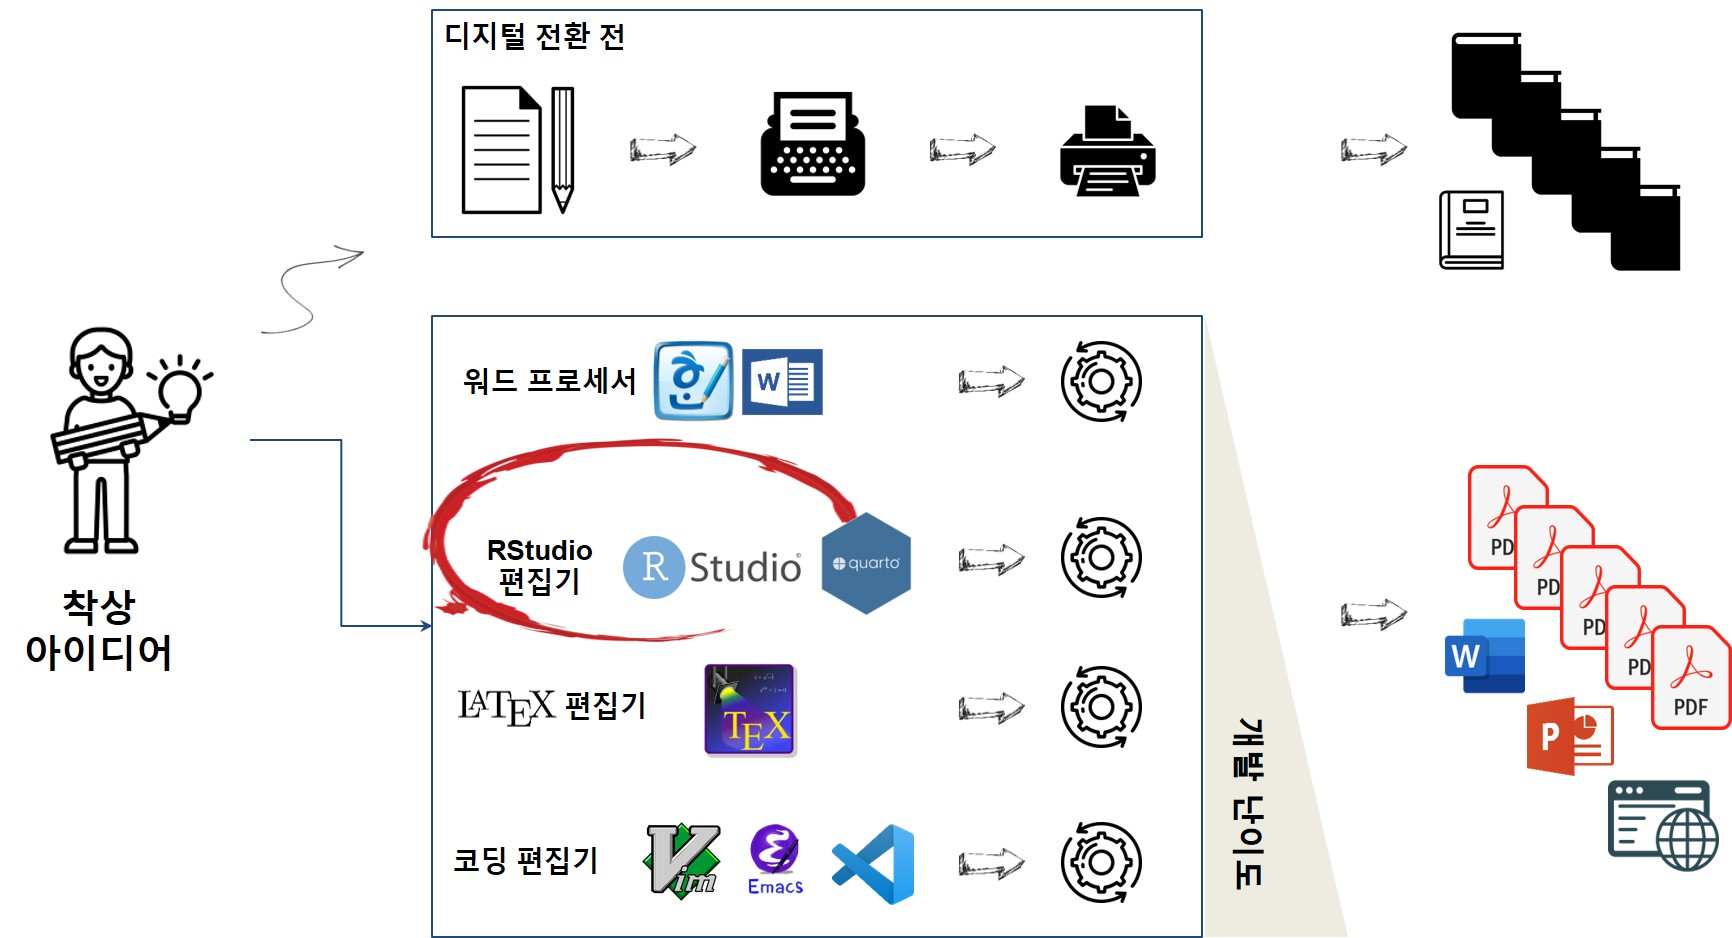
\includegraphics{images/ide_writing.jpg}

}

\caption{디지털 글쓰기 통합개발환경(IDE) 편집기}

\end{figure}

중간 단계로 \href{http://example.org}{\LaTeX}을 사용하여 수식을 포함한
학위 논문이나 학술 저널, 컨퍼런스 발표를 위한 논문을 작성하기도 한다.
이를 위해 \texttt{TeXStudio}와 같은 \href{http://example.org}{\LaTeX}에
특화된 통합개발환경(IDE)를 사용하여 생산성을 높이기도 한다. RStudio의
Visual 마크다운 편집기가 RStudio v1.4에 도입되면서, 문서 작성 방식에
혁명적 변화가 일어나고 있다. 이러한 변화를 통해 글쓰기의 생산성과
효율성이 대폭 향상되며, 다양한 포맷과 플랫폼에서의 유연한 작업이
가능해진다.

\begin{tcolorbox}[enhanced jigsaw, opacityback=0, opacitybacktitle=0.6, colback=white, rightrule=.15mm, coltitle=black, colframe=quarto-callout-note-color-frame, colbacktitle=quarto-callout-note-color!10!white, bottomrule=.15mm, bottomtitle=1mm, breakable, title=\textcolor{quarto-callout-note-color}{\faInfo}\hspace{0.5em}{통합개발환경}, titlerule=0mm, leftrule=.75mm, toptitle=1mm, left=2mm, arc=.35mm, toprule=.15mm]

통합개발환경(IDE, Integrated Development Environment)은 소프트웨어
개발을 위해 특별히 설계된 어플리케이션 또는 소프트웨어다. 코드 편집,
디버깅, 컴파일, 실행 등 소프트웨어 개발 전반을 지원한다. IDE는
프로그래밍 언어와 플랫폼에 따라 특화된 도구가 존재하고, 대표적으로 VS
코드, Eclipse, IntelliJ, Xcode, RStudio, 파이참 등이 있다.

IDE는 개발자 생산성을 높이고, 작업 효율성을 높이기 위해 자동 완성, 문법
검사, 코드 강조(Highlighting) 등 기능을 제공할 뿐만 아니라, 플러그인
형태로 버전 관리 시스템과 통합, 디버깅 툴, 테스트 자동화 도구 등도
포함되어 있다.

\end{tcolorbox}

글쓰기 IDE 도구가 필요한 이유는 단순한 텍스트 작성을 넘어서 복잡하고
기능적인 문서제작을 위해서 프로그래밍 언어와 플러그인 지원이 필수적이다.
이렇게 작성된 문서는 단순한 텍스트 제한을 벗어나 더 다양한 정보와 기능을
담게된다. 자동 완성, 문법 검사, 실시간 미리보기 등의 기능을 제공하여
문서작성 속도와 효율성이 비약적으로 높아져 생산성이 크게 향상되는데,
특히 복잡한 문서나 코드가 많이 필요한 문서를 작성할 때 시간을 대폭
줄여준다.

Git과 같은 버전 관리 시스템과 통합이 가능하므로 국내외 협업을 통해
동시에 문서 작성과 수정을 할 수 있고, 이전 버전과의 비교, 병합, 충돌
해결 등 문서 및 코드 공동 작성에서 발생하는 문제를 수월하게 해결할 수
있다. 소스코드 문서를 웹사이트(HTML), PDF, 워드 문서, 발표자료(PPT),
대쉬보드 등 다양한 파일형식으로 쉽게 변환할 수 있어해 문서 접근성을 높일
수 있고, 다양한 플랫폼에서 사용이 용이하다.

생산성을 높일 수 있는 다양한 기능을 제공하는 글쓰기 IDE 도구로 문서
작성자는 글쓰기와 고품질 문서 제작 본연의 업무에 더 많은 시간을
투여함으로써 더욱 창의적이고 효과적인 글쓰기가 가능하다.

\hypertarget{paradigm}{%
\section{저작방식 패러다임}\label{paradigm}}

\textbf{위지위그(WYSIWYG: What You See Is What You Get)}는 ``보는 대로
얻는다''는 의미로, 사용자가 문서를 편집할 때 화면에 보이는 형태가 최종
출력물과 동일하게 나오는 편집 방식이다. 대다수 현대 워드 프로세서에서
위지위그 방식을 사용하고 있다. 사용자에게 직관적이고 쉽게 접근할 수 있는
인터페이스를 제공하기 때문이다.

그러나 위지위그 방식에도 단점은 있다. 마크다운, TeX 같은 텍스트 기반
편집 방식은 문서 호환성과 범용성을 위해 쓰이는 반면, 위지위그 저작방식은
호환성과 범용성을 다소 희생할 수 밖에 없다. 특히 복잡한 문서나 웹
페이지를 작성하는 경우, 코딩방식으로 전환하여 수작업으로 최적화를
시도하더라도 완벽한 해결이 어렵다. 예를 들어, 위지위그 편집기에서 문서를
작성하면 뒷단에 불필요한 코드나 태그가 자동으로 생성되어 문서 최적화를
방해하며, 시간이 지남에 따라 누적되어 호환성과 재현성에 심각한 문제를
야기한다. \footnote{\href{https://ko.wikipedia.org/wiki/\%EC\%9C\%84\%EC\%A7\%80\%EC\%9C\%84\%EA\%B7\%B8}{위키백과,
  ``위지위그''}} \footnote{\href{https://namu.wiki/w/WYSIWYG}{나무위키,
  ``WYSIWYG''}}

\textbf{위지윔(WYSIWYM: What You See Is What You Mean)}은 ``당신이 보는
것은 당신이 뜻하는 것이다''라는 의미로, 위지위그(WYSIWYG) 방식의 한계를
극복하기 위해 나온 대안 편집 방식이다. 위지윔 방식에서는 사용자가 무엇을
의미하는지를 중점으로 두어, 본래의 코드 구조를 더 명확하게 알 수 있다.
코드 의미를 직접적으로 반영하여, 불필요한 요소 없이 효율적으로 문서를
작성할 수 있는 장점이 있다.

RStudio의 Visual 편집 기능은 위지윔 지향점을 잘 반영하고 있다. 사용자는
복잡한 코드나 태그 없이도 의미 있는 문서 구조를 쉽게 생성하고 관리할 수
있어 문서 최적화와 호환성을 높일 수 있으며, 더욱 높은 문서 저작 생산성을
달성할 수 있다.

오픈 소스 LaTeX 편집기인 \href{https://www.lyx.org/}{LyX}는 위지윔
방식을 초기부터 채택하여 사용자에게 코드 본래 구조와 의미를 명확하게
파악할 수 있는 인터페이스를 제공했다. 이러한 접근법은 복잡한 수식이나
과학적인 문서를 작성할 때 특히 유용하며,
\href{http://example.org}{\LaTeX} 복잡성을 낮추면서도 강력한 기능을
최대한 활용할 수 함으로써 위지위그 한계를 극복했다는 평가를 받고 있다.

\begin{longtable}[]{@{}
  >{\centering\arraybackslash}p{(\columnwidth - 2\tabcolsep) * \real{0.5278}}
  >{\centering\arraybackslash}p{(\columnwidth - 2\tabcolsep) * \real{0.4722}}@{}}
\toprule\noalign{}
\begin{minipage}[b]{\linewidth}\centering
문서 컴파일
\end{minipage} & \begin{minipage}[b]{\linewidth}\centering
위지위그
\end{minipage} \\
\midrule\noalign{}
\endhead
\bottomrule\noalign{}
\endlastfoot
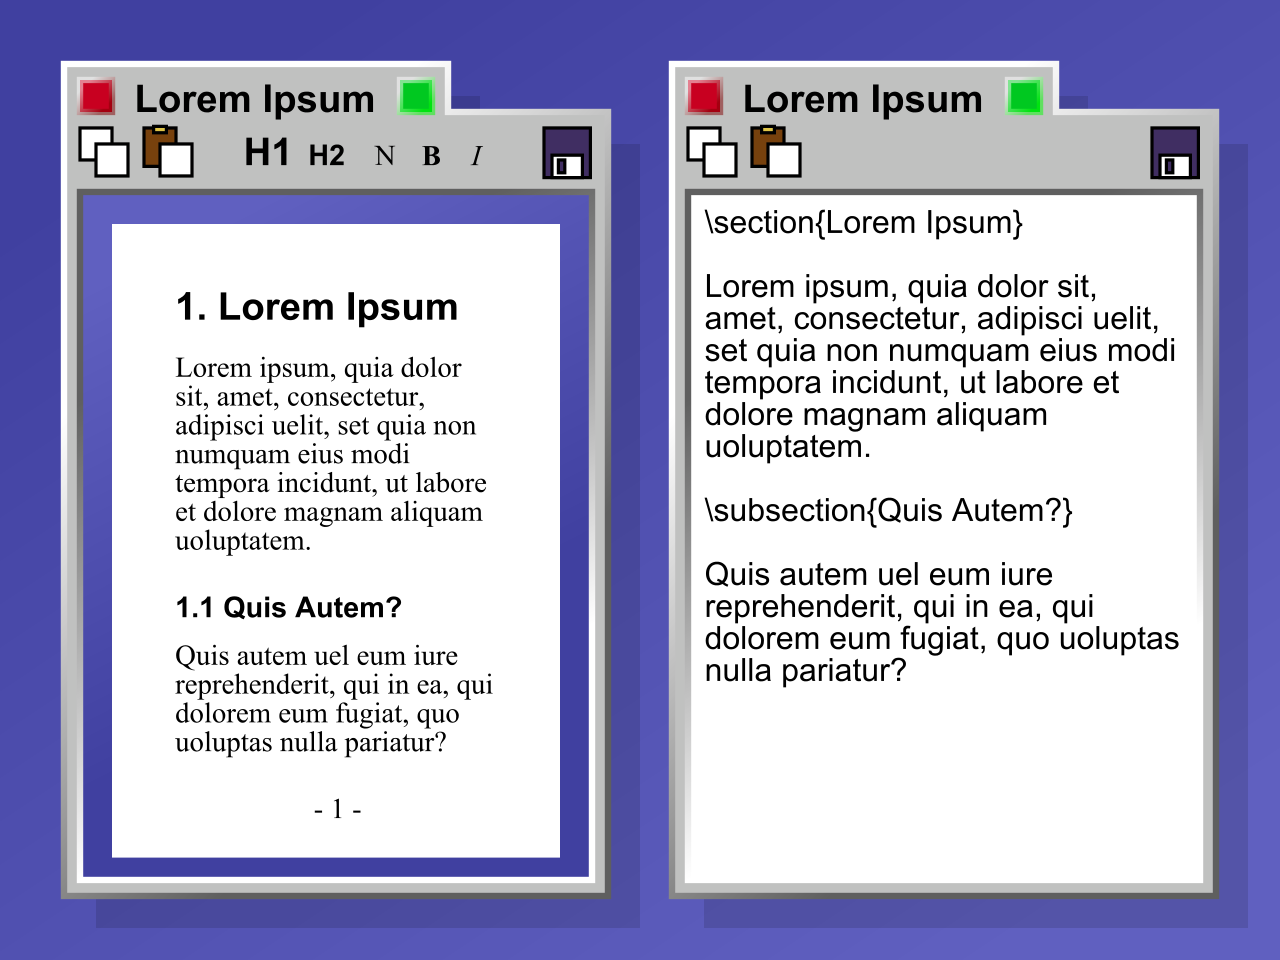
\includegraphics[width=2.60417in,height=\textheight]{images/wyswig-wikipedia.png}
&
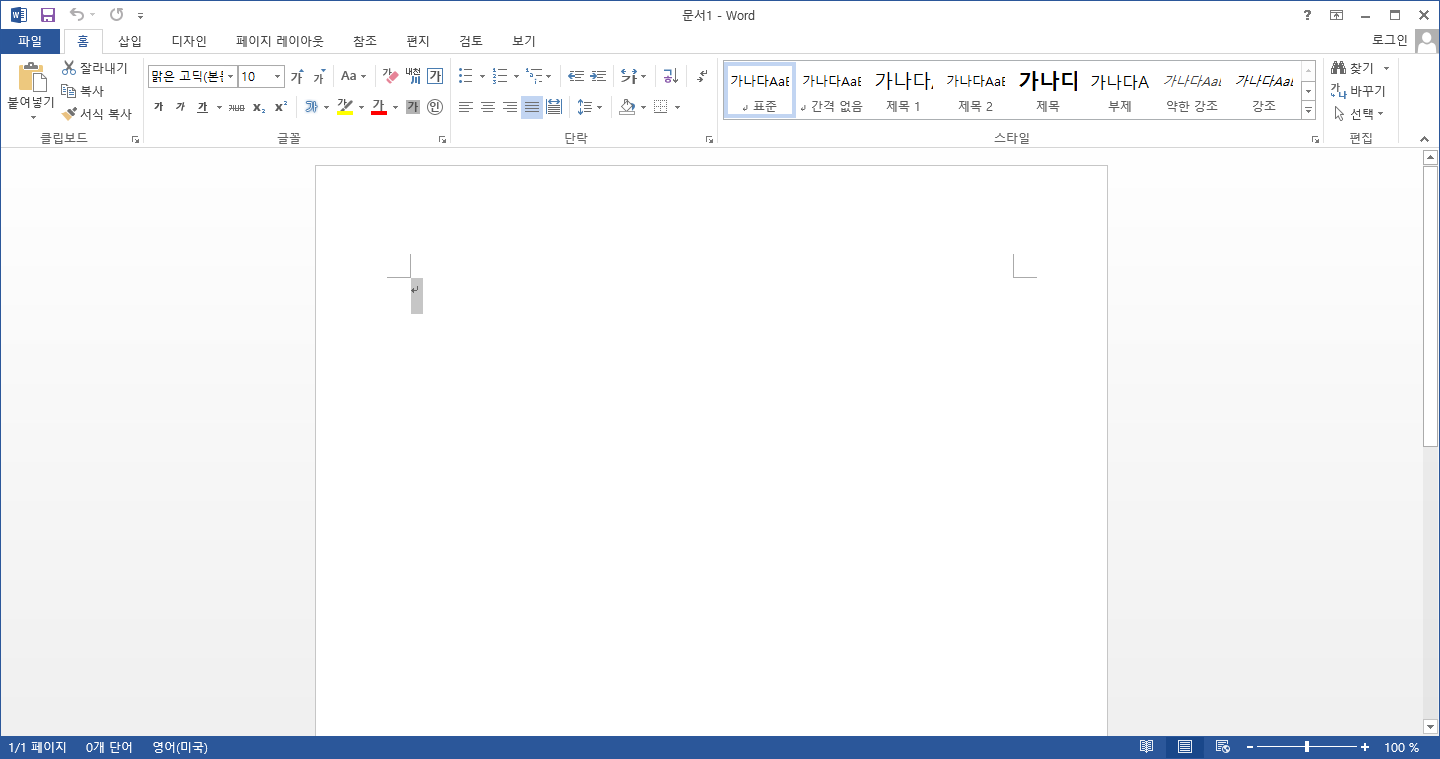
\includegraphics[width=2.60417in,height=\textheight]{images/wyswyg-word.png} \\
\end{longtable}

\hypertarget{main-features}{%
\section[워드 프로세서 ]{\texorpdfstring{워드 프로세서
\footnote{\href{https://www.educba.com/microsoft-word-features/}{Jesal
  Shethna, ``Microsoft Word Features'', EDUCBA}}}{워드 프로세서 }}\label{main-features}}

\textbf{워드 프로세서(Word Processor)}는 문서 제작을 위한 소프트웨어로,
시각적으로 잘 구성된 인터페이스와 다양한 편집 기능을 제공한다. 사용자는
이러한 기능을 통해 원하는 형태와 구조를 갖는 문서를 쉽게 저작할 수 있다.
워드 프로세서는 글자 스타일, 문단 구성, 이미지 삽입, 표 만들기 등 다양한
기능이 포괄적으로 제공되며, 윈도우에 기본 제공되는 메모장(Notepad)
텍스트 편집기보다 훨씬 더 풍부한 문서 작성이 가능하다. 2023년 9월
1일부로 윈도우에서 무료로 제공되던 워드패드(WordPad)에 대한 지원도
없어지고 윈도우에서도 제거될 것이라는 발표가 있었다. 따라서, 서식이
필요한 문서를 저작할 경우 MS 워드(Word)나 아래한글과 같은 워드
프로세서를 사용해야 된다.

아래한글은 국내에서 널리 사용되는 워드 프로세서 중 하나로, 한국 문화와
업무 환경에 맞춰 특화된 기능을 제공한다. 정부나 공공기관에서 사용하는
특별한 문서 양식을 미리 저장해 두어, 사용자가 양식을 찾는 데 시간을 쓰지
않고 글쓰기에 바로 집중할 수 있도록 큰 도움을 주었다.

\begin{longtable}[]{@{}
  >{\centering\arraybackslash}p{(\columnwidth - 2\tabcolsep) * \real{0.5278}}
  >{\centering\arraybackslash}p{(\columnwidth - 2\tabcolsep) * \real{0.4722}}@{}}
\toprule\noalign{}
\begin{minipage}[b]{\linewidth}\centering
국산 워드 프로세서
\end{minipage} & \begin{minipage}[b]{\linewidth}\centering
해외 워드 프로세서
\end{minipage} \\
\midrule\noalign{}
\endhead
\bottomrule\noalign{}
\endlastfoot
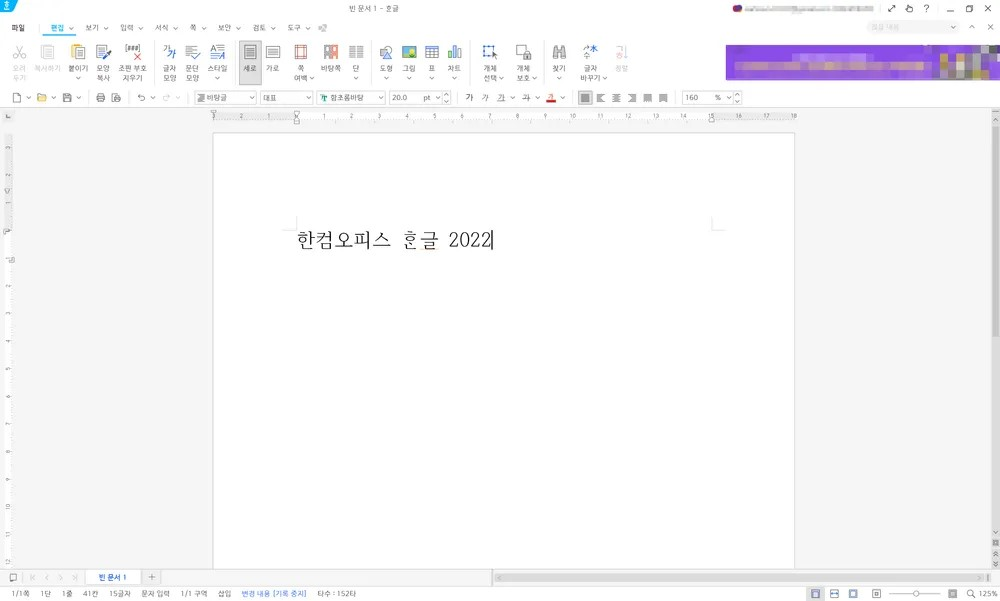
\includegraphics[width=5.20833in,height=\textheight]{images/hangul_word.jpg}
&
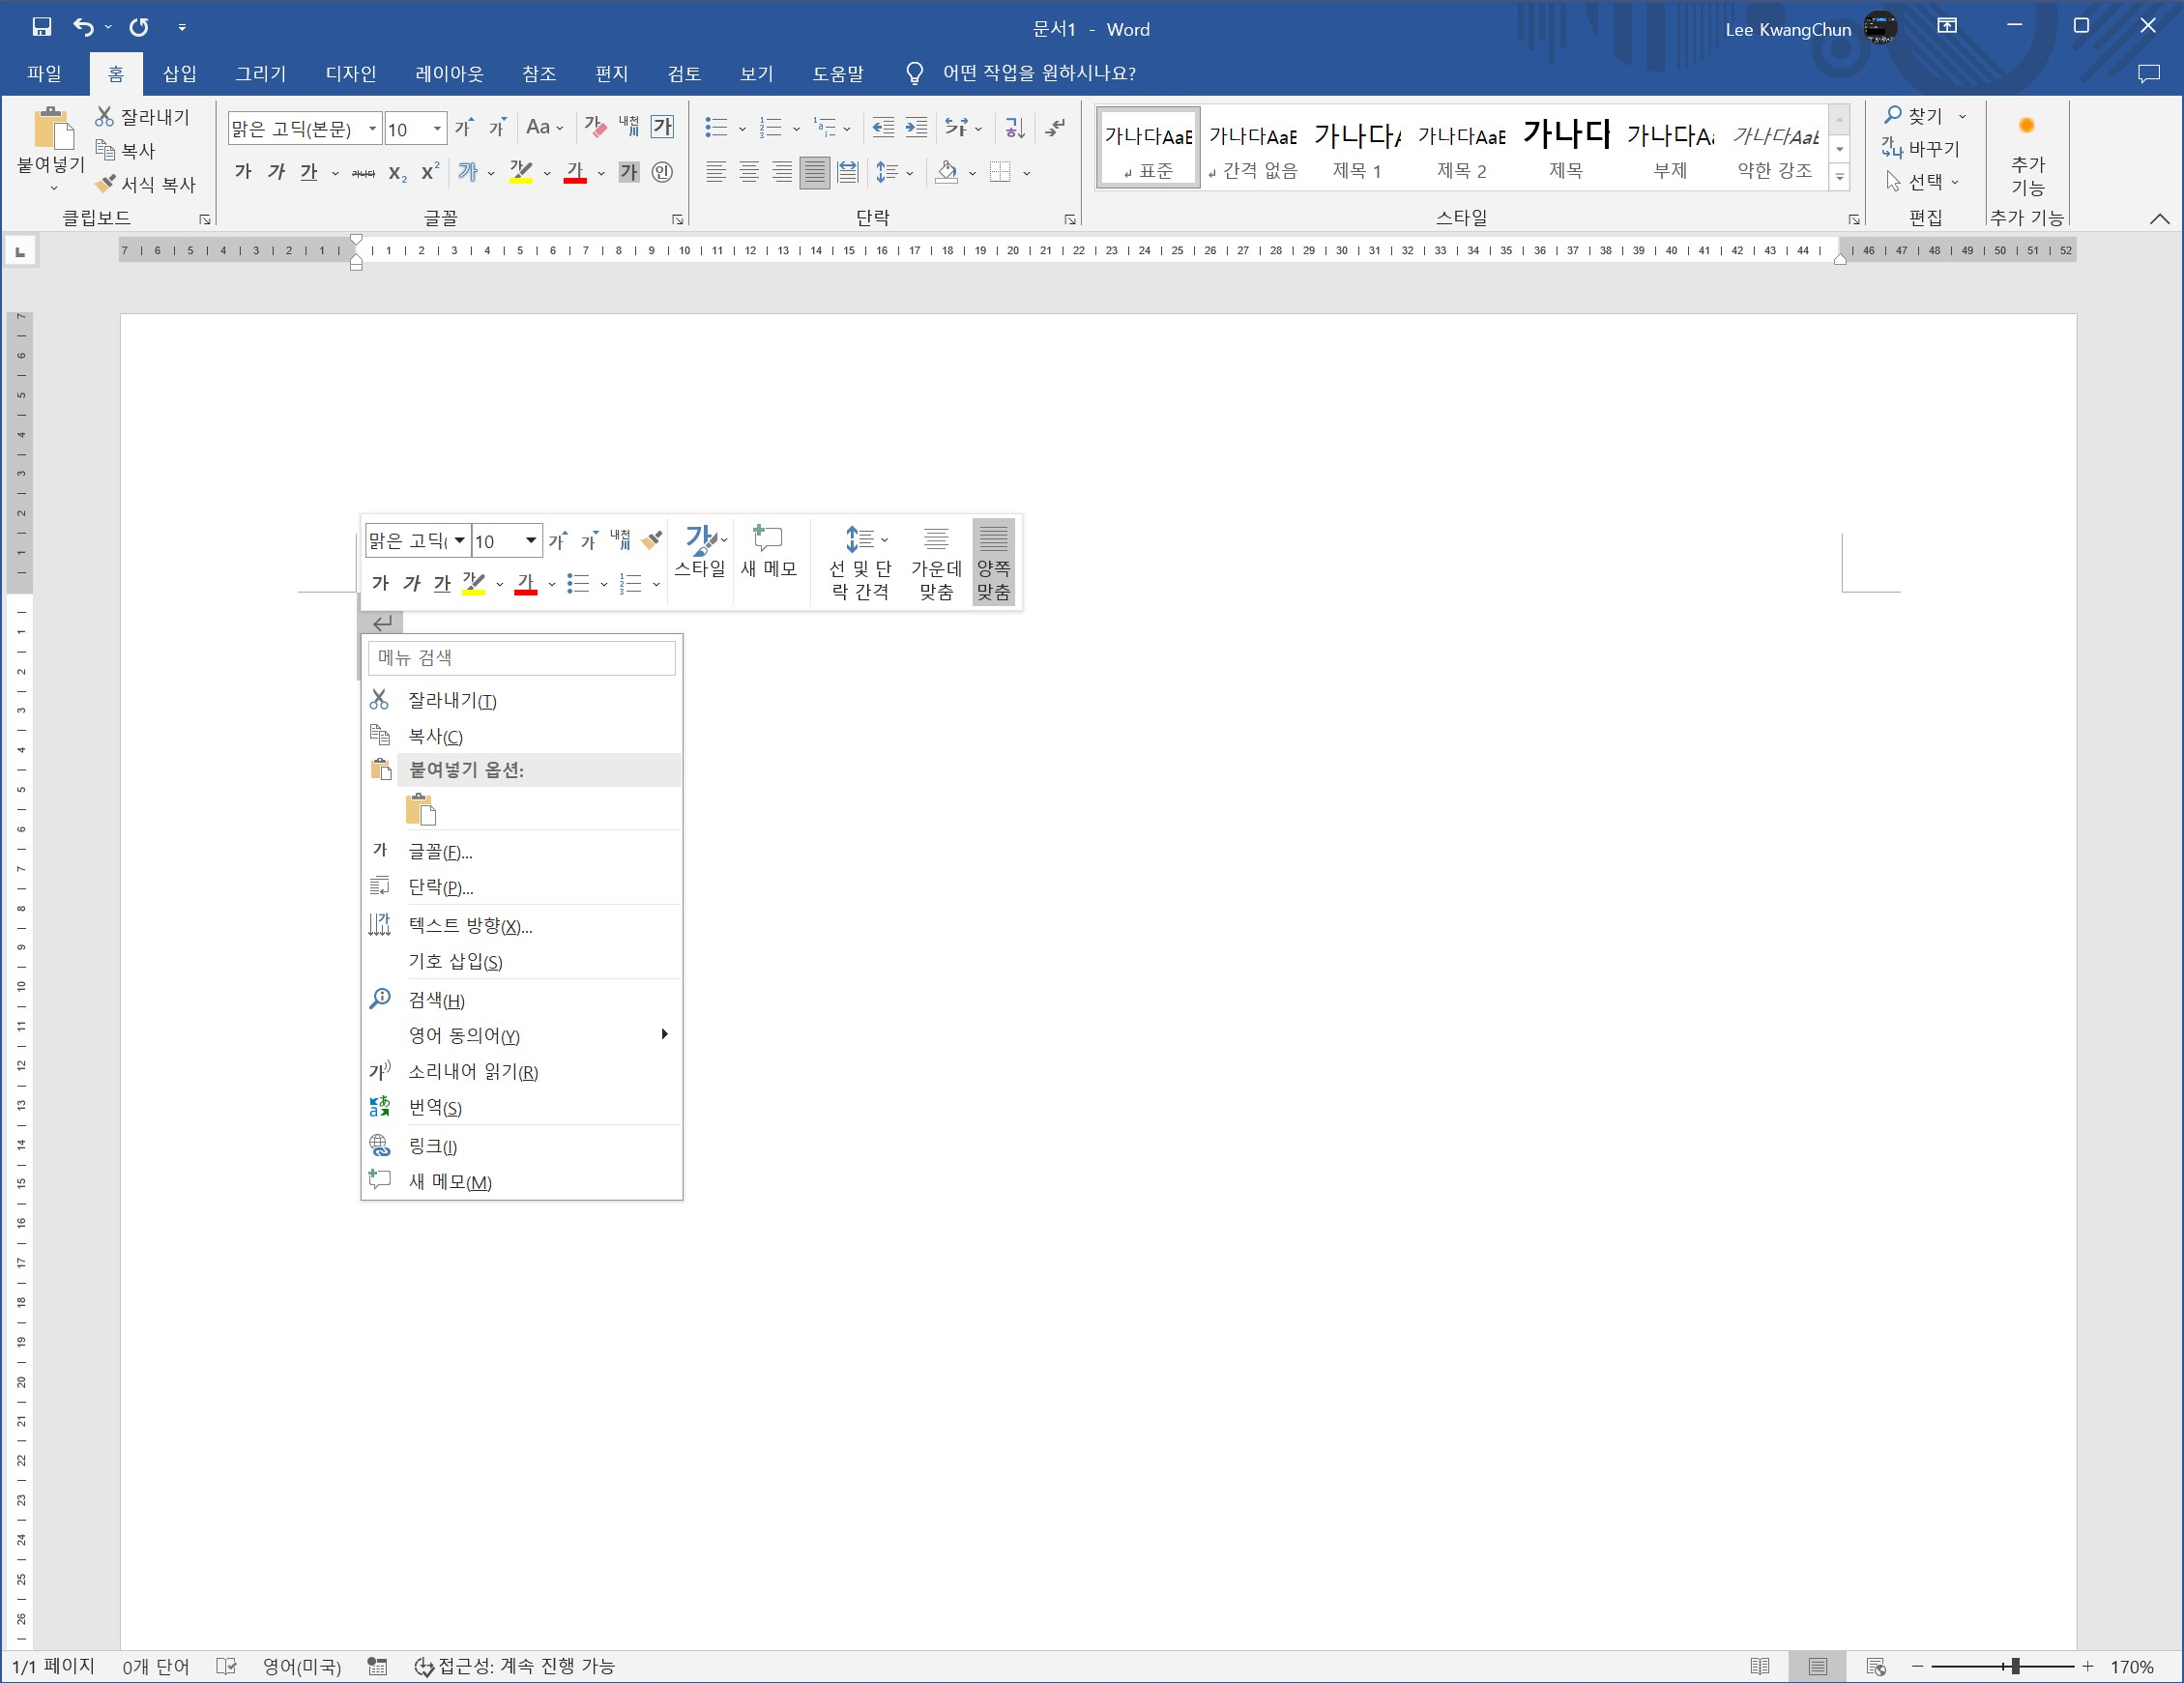
\includegraphics[width=5.20833in,height=\textheight]{images/word_ms.jpg} \\
\end{longtable}

\hypertarget{latex-editor}{%
\section{\texorpdfstring{\href{http://example.org}{\LaTeX}
편집기}{ 편집기}}\label{latex-editor}}

\href{http://example.org}{\LaTeX} 편집기는 운영체제나 사용자의 필요에
따라 다양한 선택옵션이 존재한다. 특히, 클라우드 기반
\href{https://www.overleaf.com/}{Overleaf}, 설치형
\href{https://www.texstudio.org/}{TeXstudio}, 데이터 과학에 특화된
RStudio IDE가 대표적이다. 편집기들은 \href{http://example.org}{\LaTeX}에
특화되었거나, 일부 \href{http://example.org}{\LaTeX} 기능을 분리하여
사용자 요구에 맞춰 활용할 수 있다.

\begin{figure}

{\centering 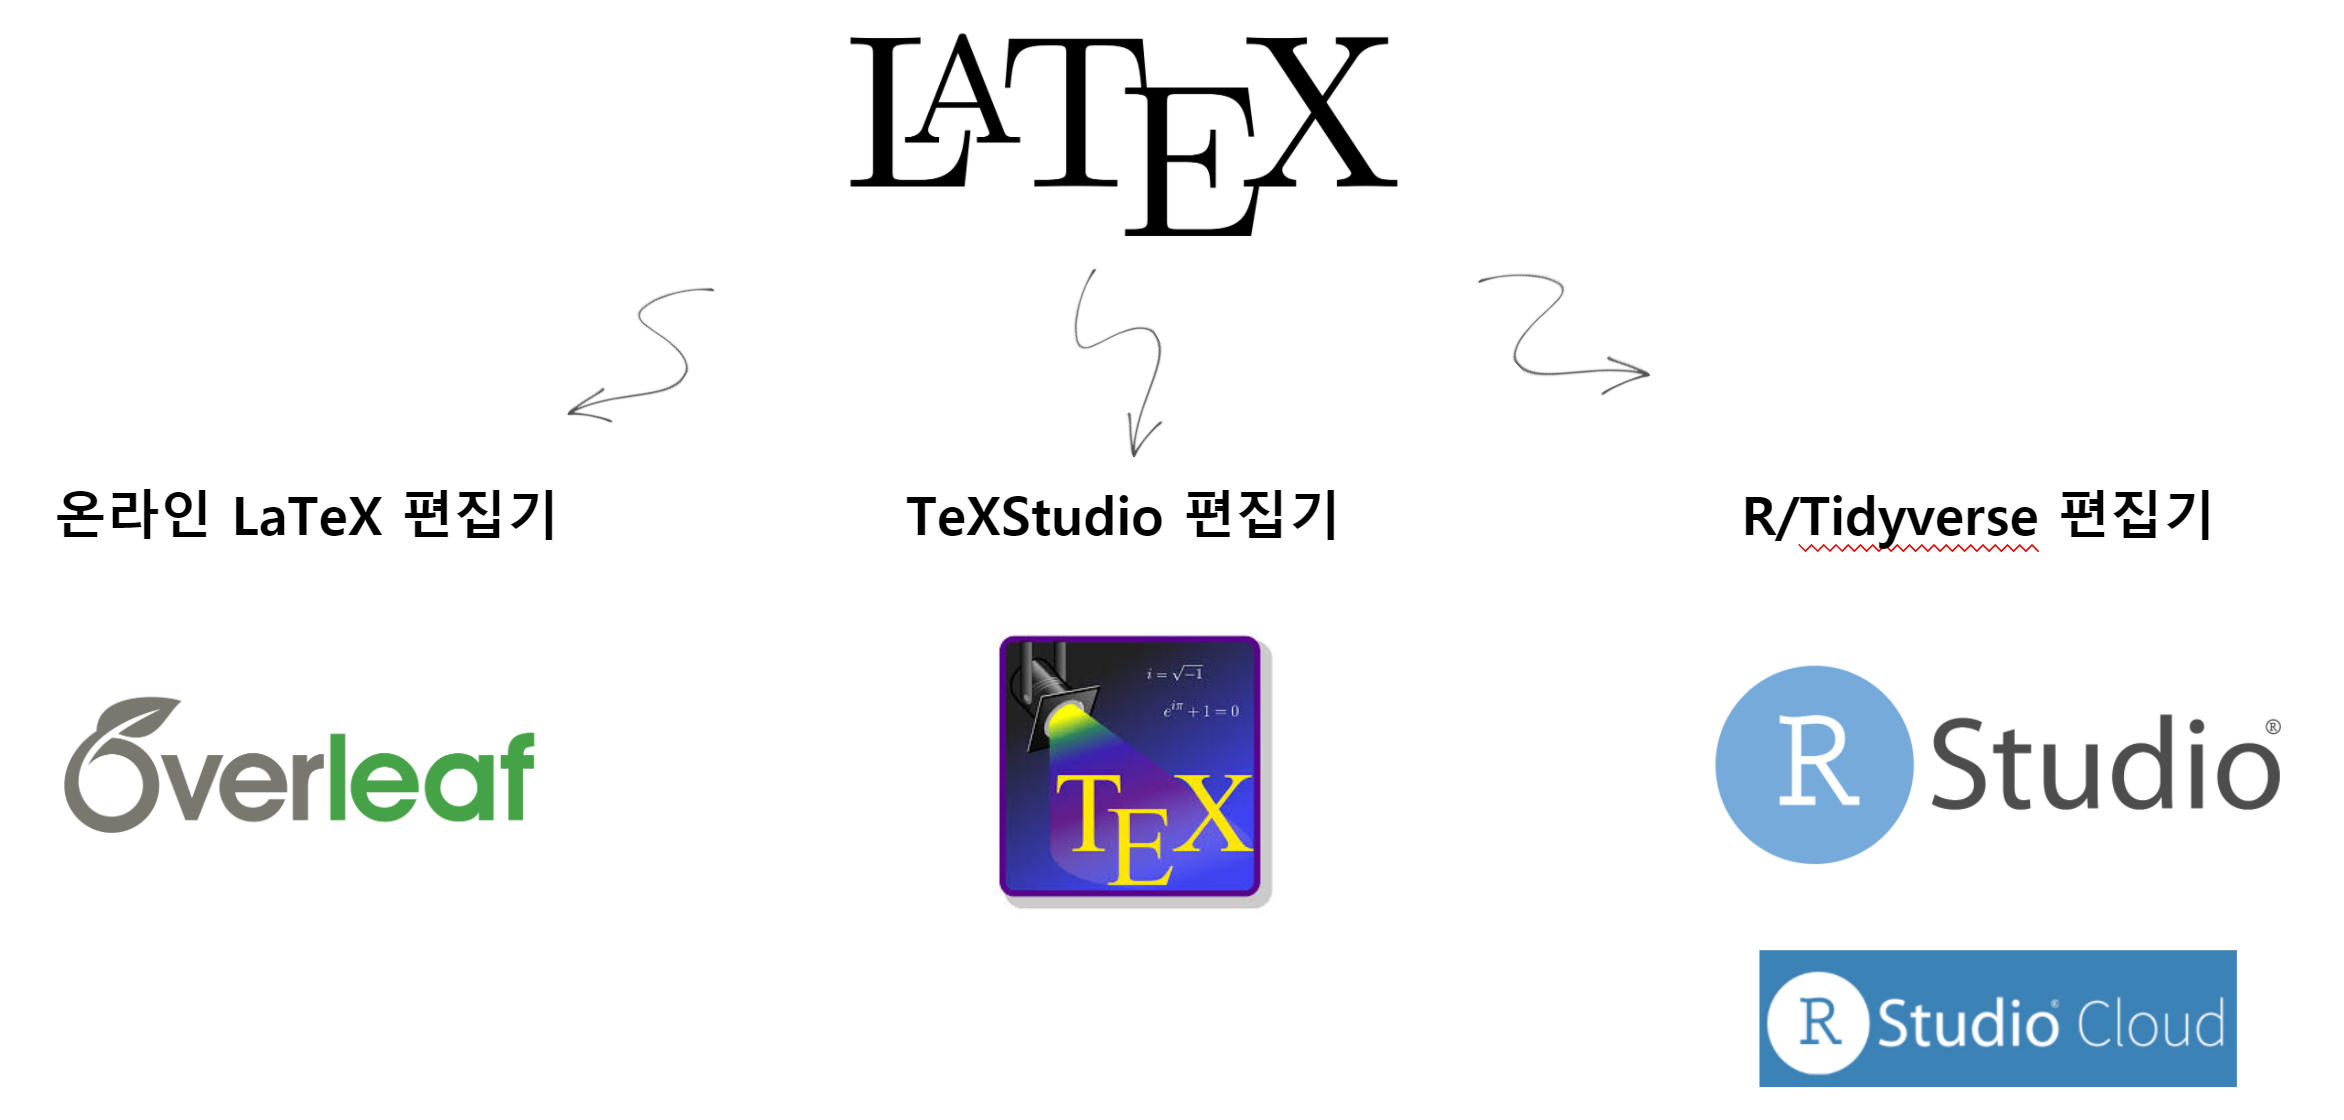
\includegraphics[width=11.98958in,height=\textheight]{images/latex-editor.png}

}

\caption{\href{http://example.org}{\LaTeX} 편집기 다양성}

\end{figure}

\href{https://www.overleaf.com/}{Overleaf}는 초기에 \texttt{ShareLaTeX}
서비스로 시작해 현재는 클라우드 기반의 \href{http://example.org}{\LaTeX}
편집 기능을 제공한다. 클라우드 특성을 살려 문서의 공유와 협업이
용이하다는 점이 큰 장점이다.

\texttt{TeXstudio}는 \texttt{Texmaker} 후속으로 오픈 소스
\href{http://example.org}{\LaTeX} 편집기로 제공된다. 사용자는
\href{https://www.texstudio.org/}{TeXstudio} 웹사이트에서 다운로드 받아
설치할 수 있으며, GitHub
\href{https://github.com/texstudio-org/texstudio}{\texttt{texstudio}}
저장소를 통해 한국어 현지화 작업에도 참여할 수 있다.

\begin{longtable}[]{@{}
  >{\centering\arraybackslash}p{(\columnwidth - 2\tabcolsep) * \real{0.5278}}
  >{\centering\arraybackslash}p{(\columnwidth - 2\tabcolsep) * \real{0.4722}}@{}}
\toprule\noalign{}
\begin{minipage}[b]{\linewidth}\centering
클라우드 편집기
\end{minipage} & \begin{minipage}[b]{\linewidth}\centering
설치형 편집기
\end{minipage} \\
\midrule\noalign{}
\endhead
\bottomrule\noalign{}
\endlastfoot
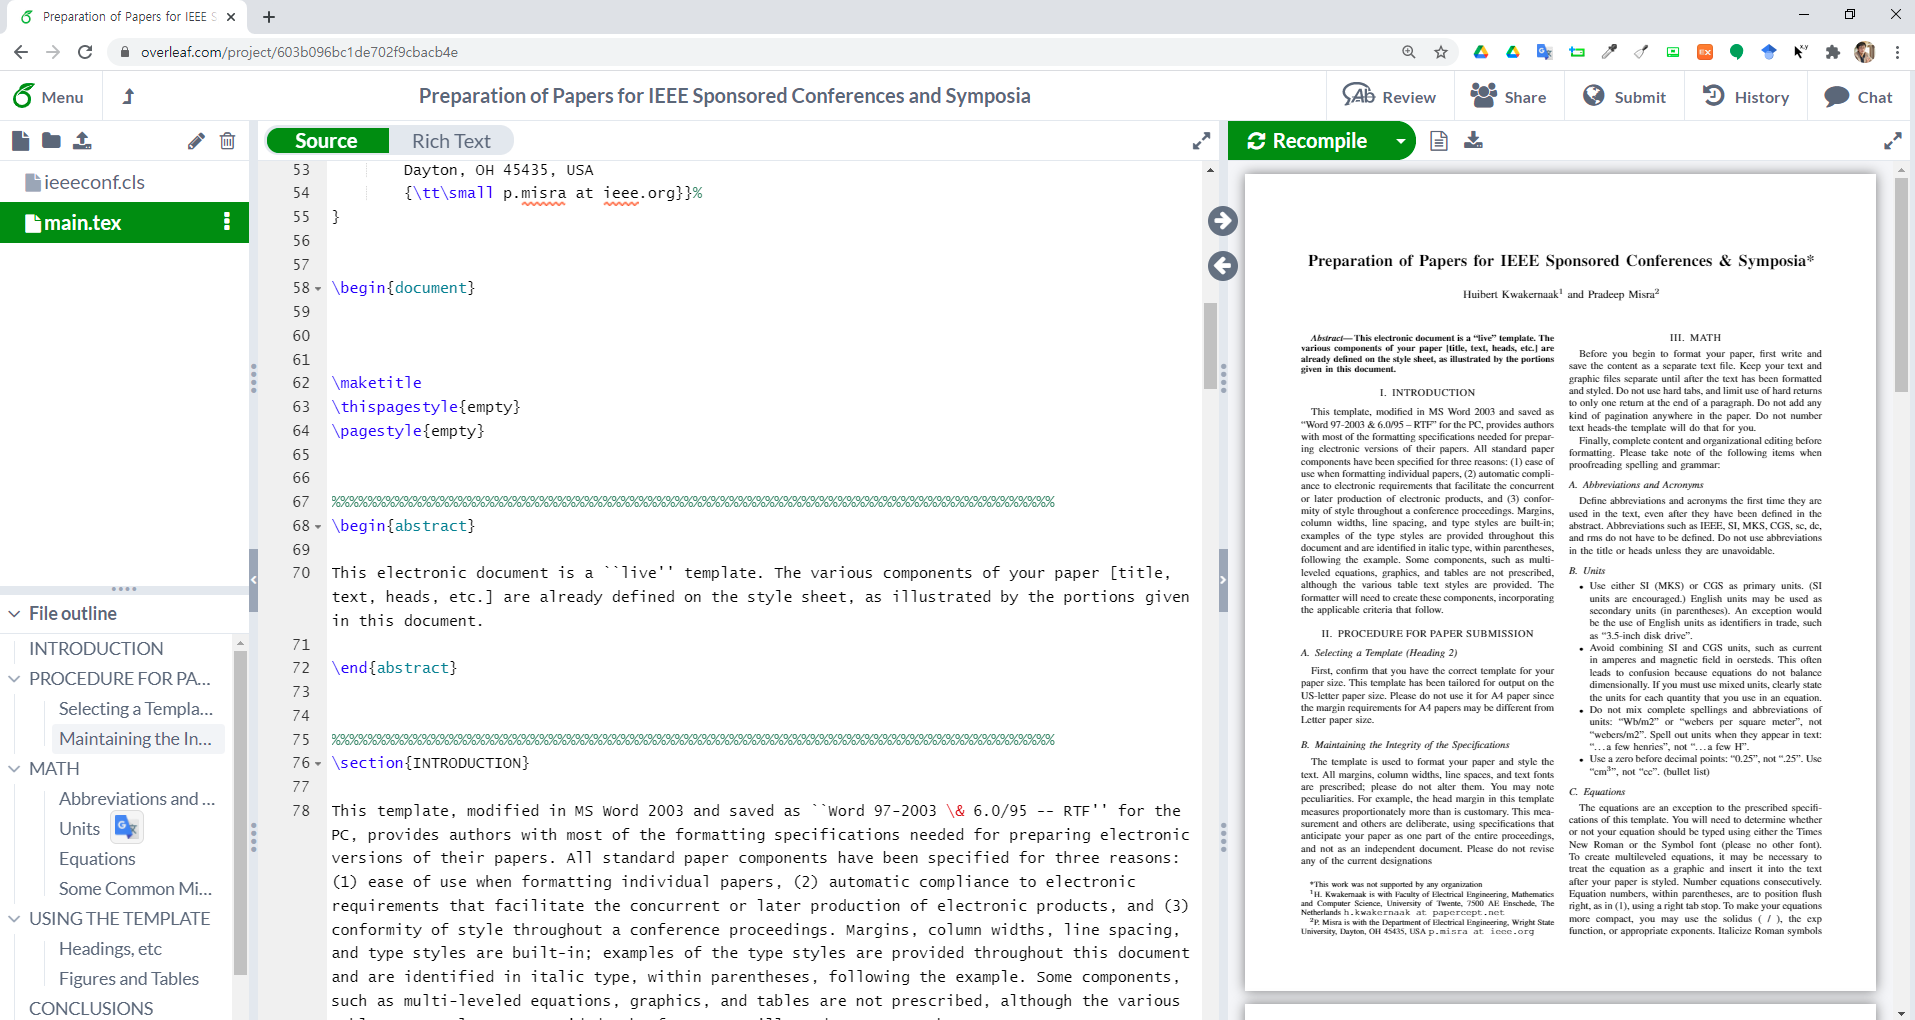
\includegraphics[width=5.20833in,height=\textheight]{images/overleaf-screenshot.png}
&
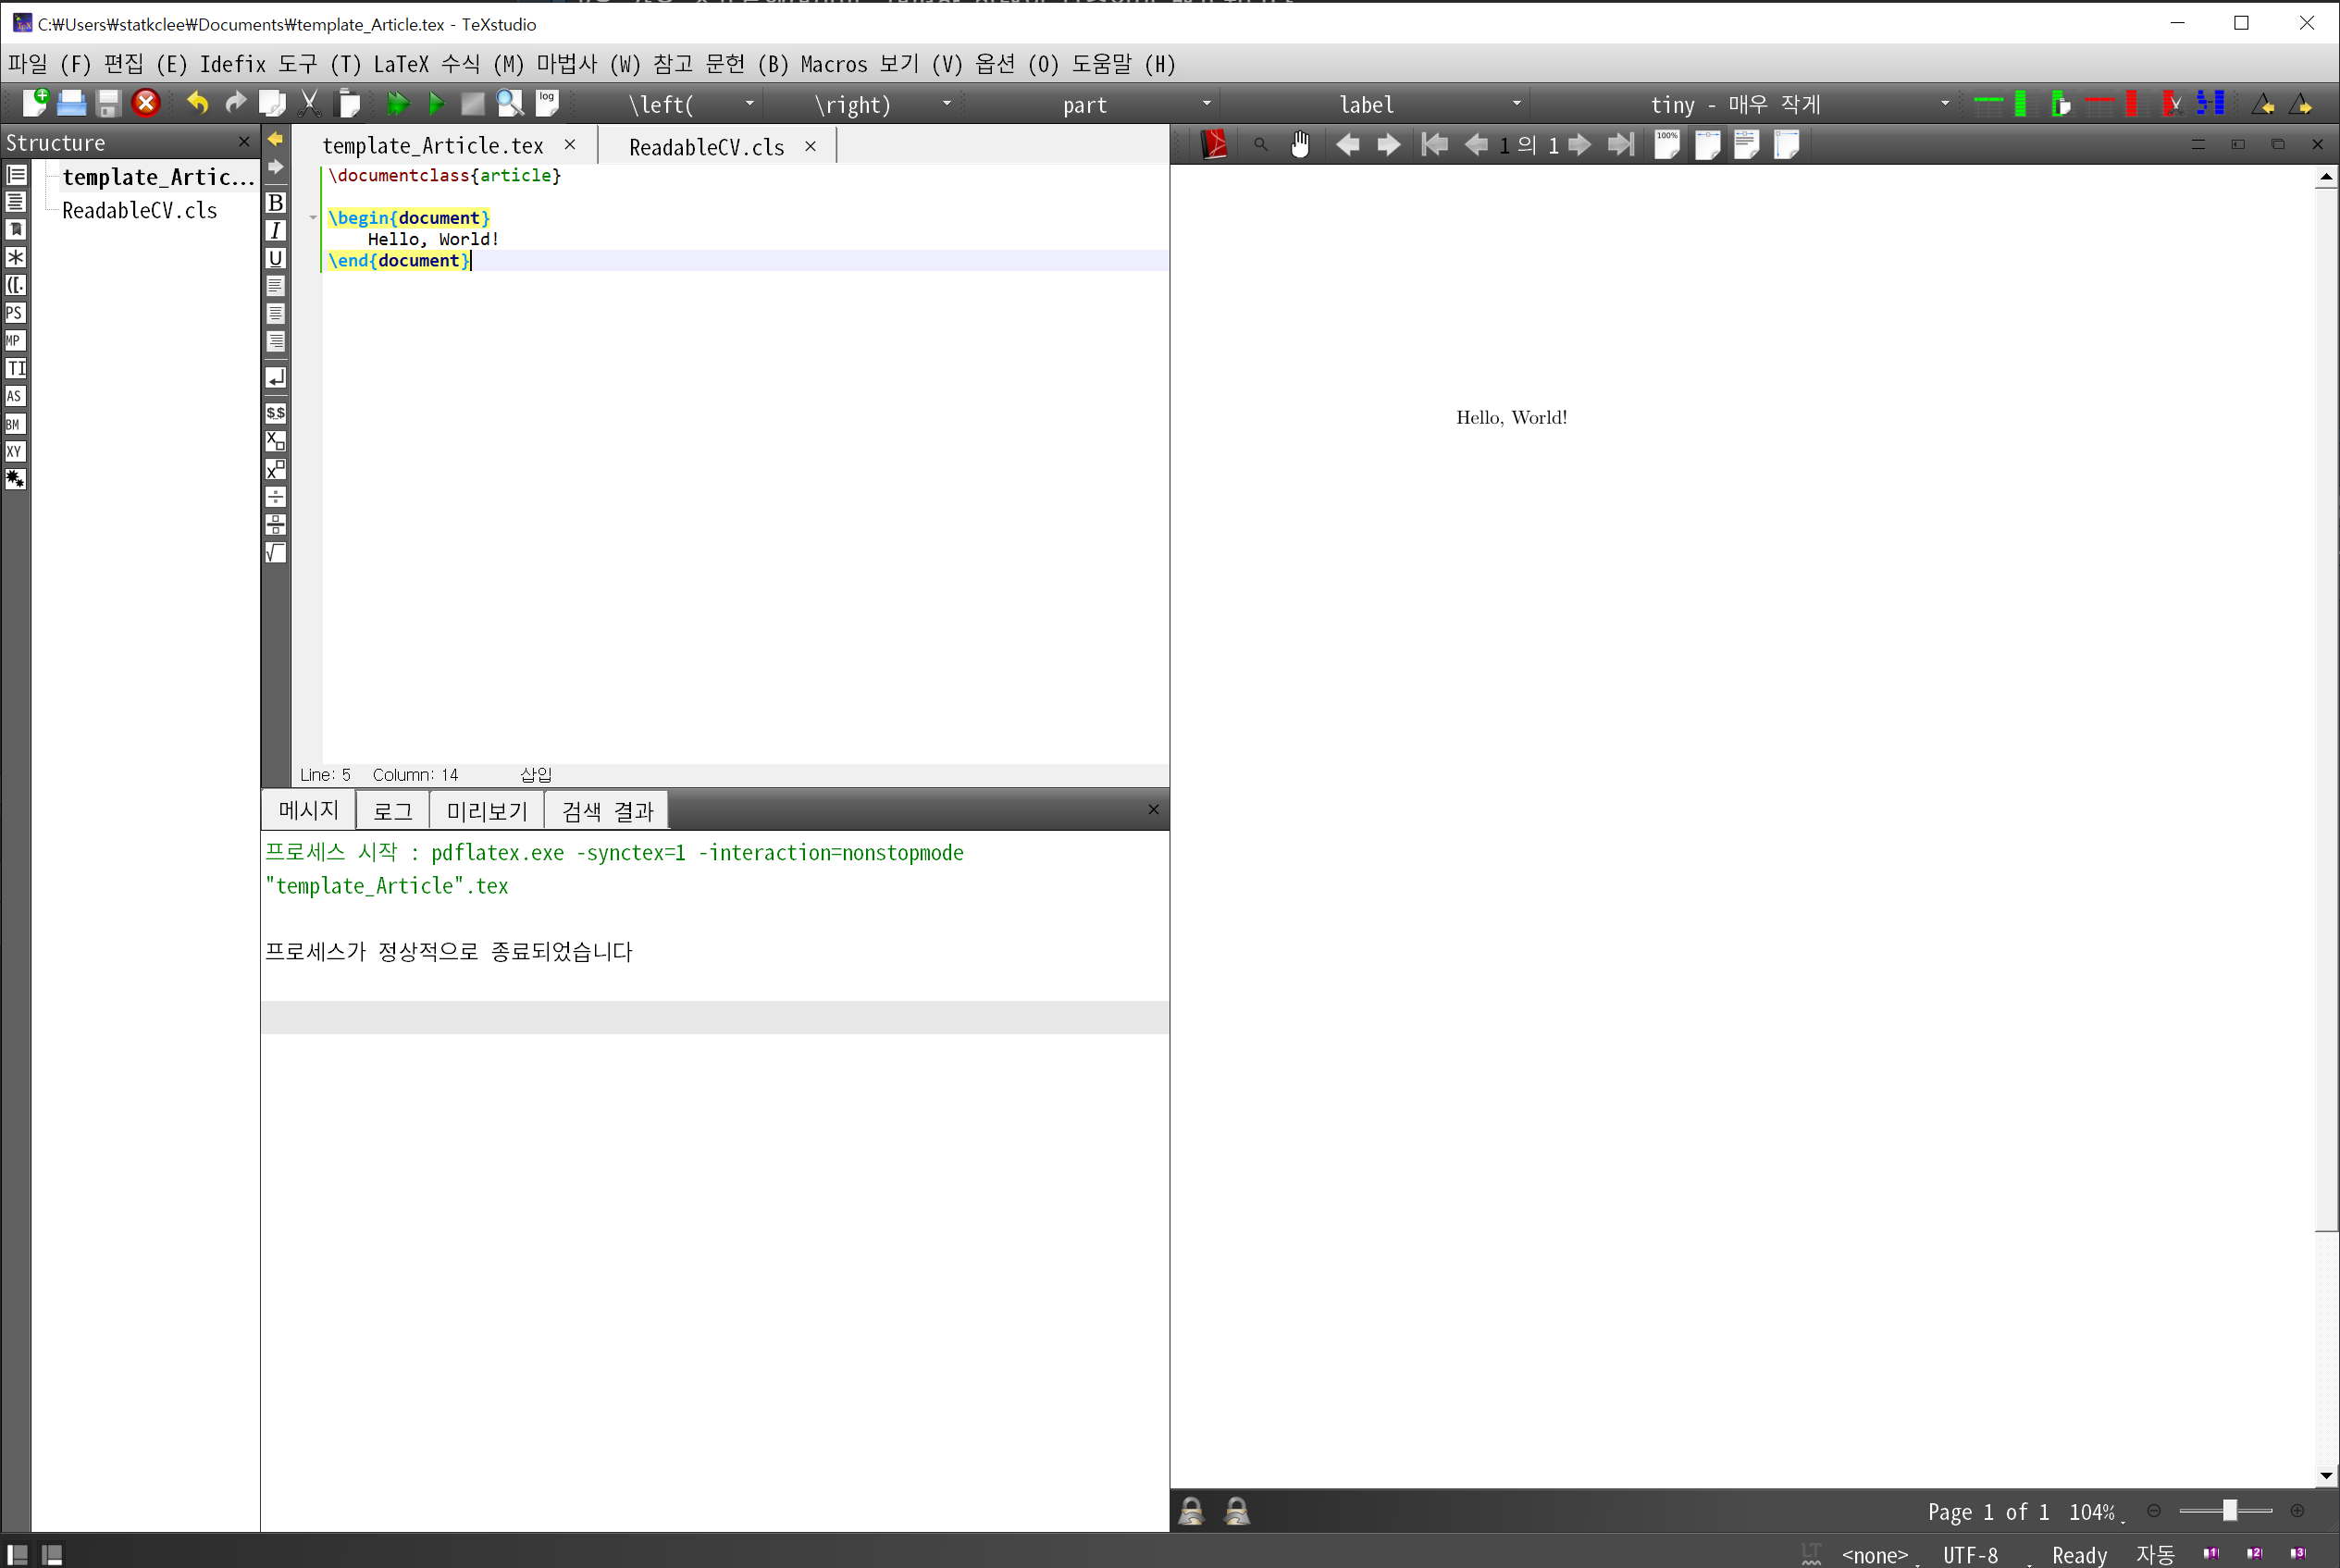
\includegraphics[width=5.20833in,height=\textheight]{images/texstudio-screenshot.png} \\
\end{longtable}

\hypertarget{rstudio-ide}{%
\section{RStudio IDE 편집기}\label{rstudio-ide}}

RStudio IDE는 처음 데이터 과학 R 프로그래밍 언어를 위한 통합개발환경으로
시작하였으나 이제는 파이썬을 비롯하여 SQL, Observable JS 등 데이터 과학
전분야를 담당하고 있다. 특히, 데이터 분석, 시각화 및 문서 작업을
간편하게 할 수 있도록 다양한 도구와 기능을 제공할 뿐만 아니라, Shiny 웹
애플리케이션 개발, Plumber를 통한 API 개발, 쿼토(Quarto)/R 마크다운을
활용해 다양한 데이터 과학 산출물을 제작할 수 있다. 또한, Git 버전 관리
시스템과 통합되어 코드 이력을 쉽게 추적하고 관리할 수 있고 GitHub과
연결하여 협업기능도 지원한다.

RStudio 코드 편집기는 자동 완성, 구문 강조, 맞춤법 검사 등 기능을
제공하여 개발자 편의를 향상시켰고, GUI 데이터 뷰어를 통해 데이터프레임과
데이터 객체를 직접적으로 시각적으로 살펴볼 수 있으며, 내장 패키지 관리
시스템을 통해 R 패키지도 손쉽게 설치하고 관리할 수 있다.

웹앱 Shiny 애플리케이션 개발과 테스트도 가능하고, 문서화 프로그래밍을
차세대 R 마크다운 쿼토(Quarto)를 이용하여 코드, 데이터, 그래프를 하나의
문서로 통합하여 구현할 수 있을 뿐만 아니라 팬독(Pandoc)을 통해 다양한
형태 문서를 자동으로 생성할 수 있다.

\begin{figure}

{\centering 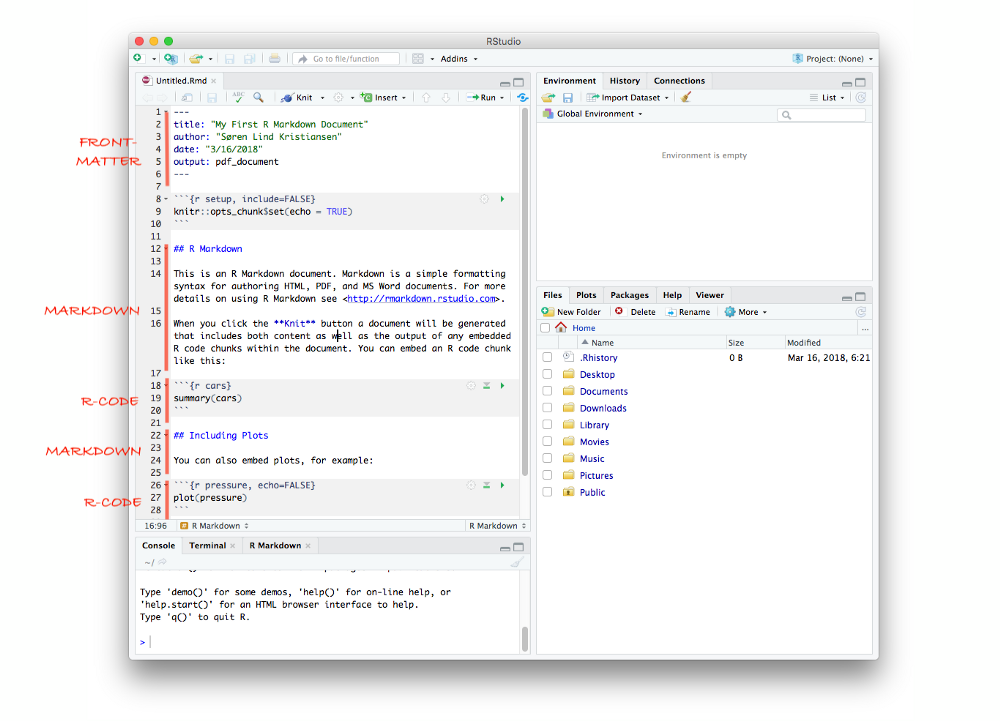
\includegraphics[width=7.94792in,height=\textheight]{images/rstudio-screenshot.png}

}

\caption{RStudio 문서화 프로그래밍 사례}

\end{figure}

\hypertarget{visual-markdown-main-features}{%
\subsection{Visual 마크다운
편집기}\label{visual-markdown-main-features}}

\href{https://rstudio.github.io/visual-markdown-editing}{Visual
마크다운} 기능을 사용하게 되면 과학/기술 문서 작성의 용이성 뿐만 아니라
인용(Citation), 문학적 프로그래밍(literate programming) 을 통한
재현가능한 과학문서 구현, 팬독(\texttt{Pandoc})을 사용하여 텍스트와
코드로 PDF, HTML, 워드 등 다양한 문서 동시 생성이 가능하다.

\begin{figure}

{\centering 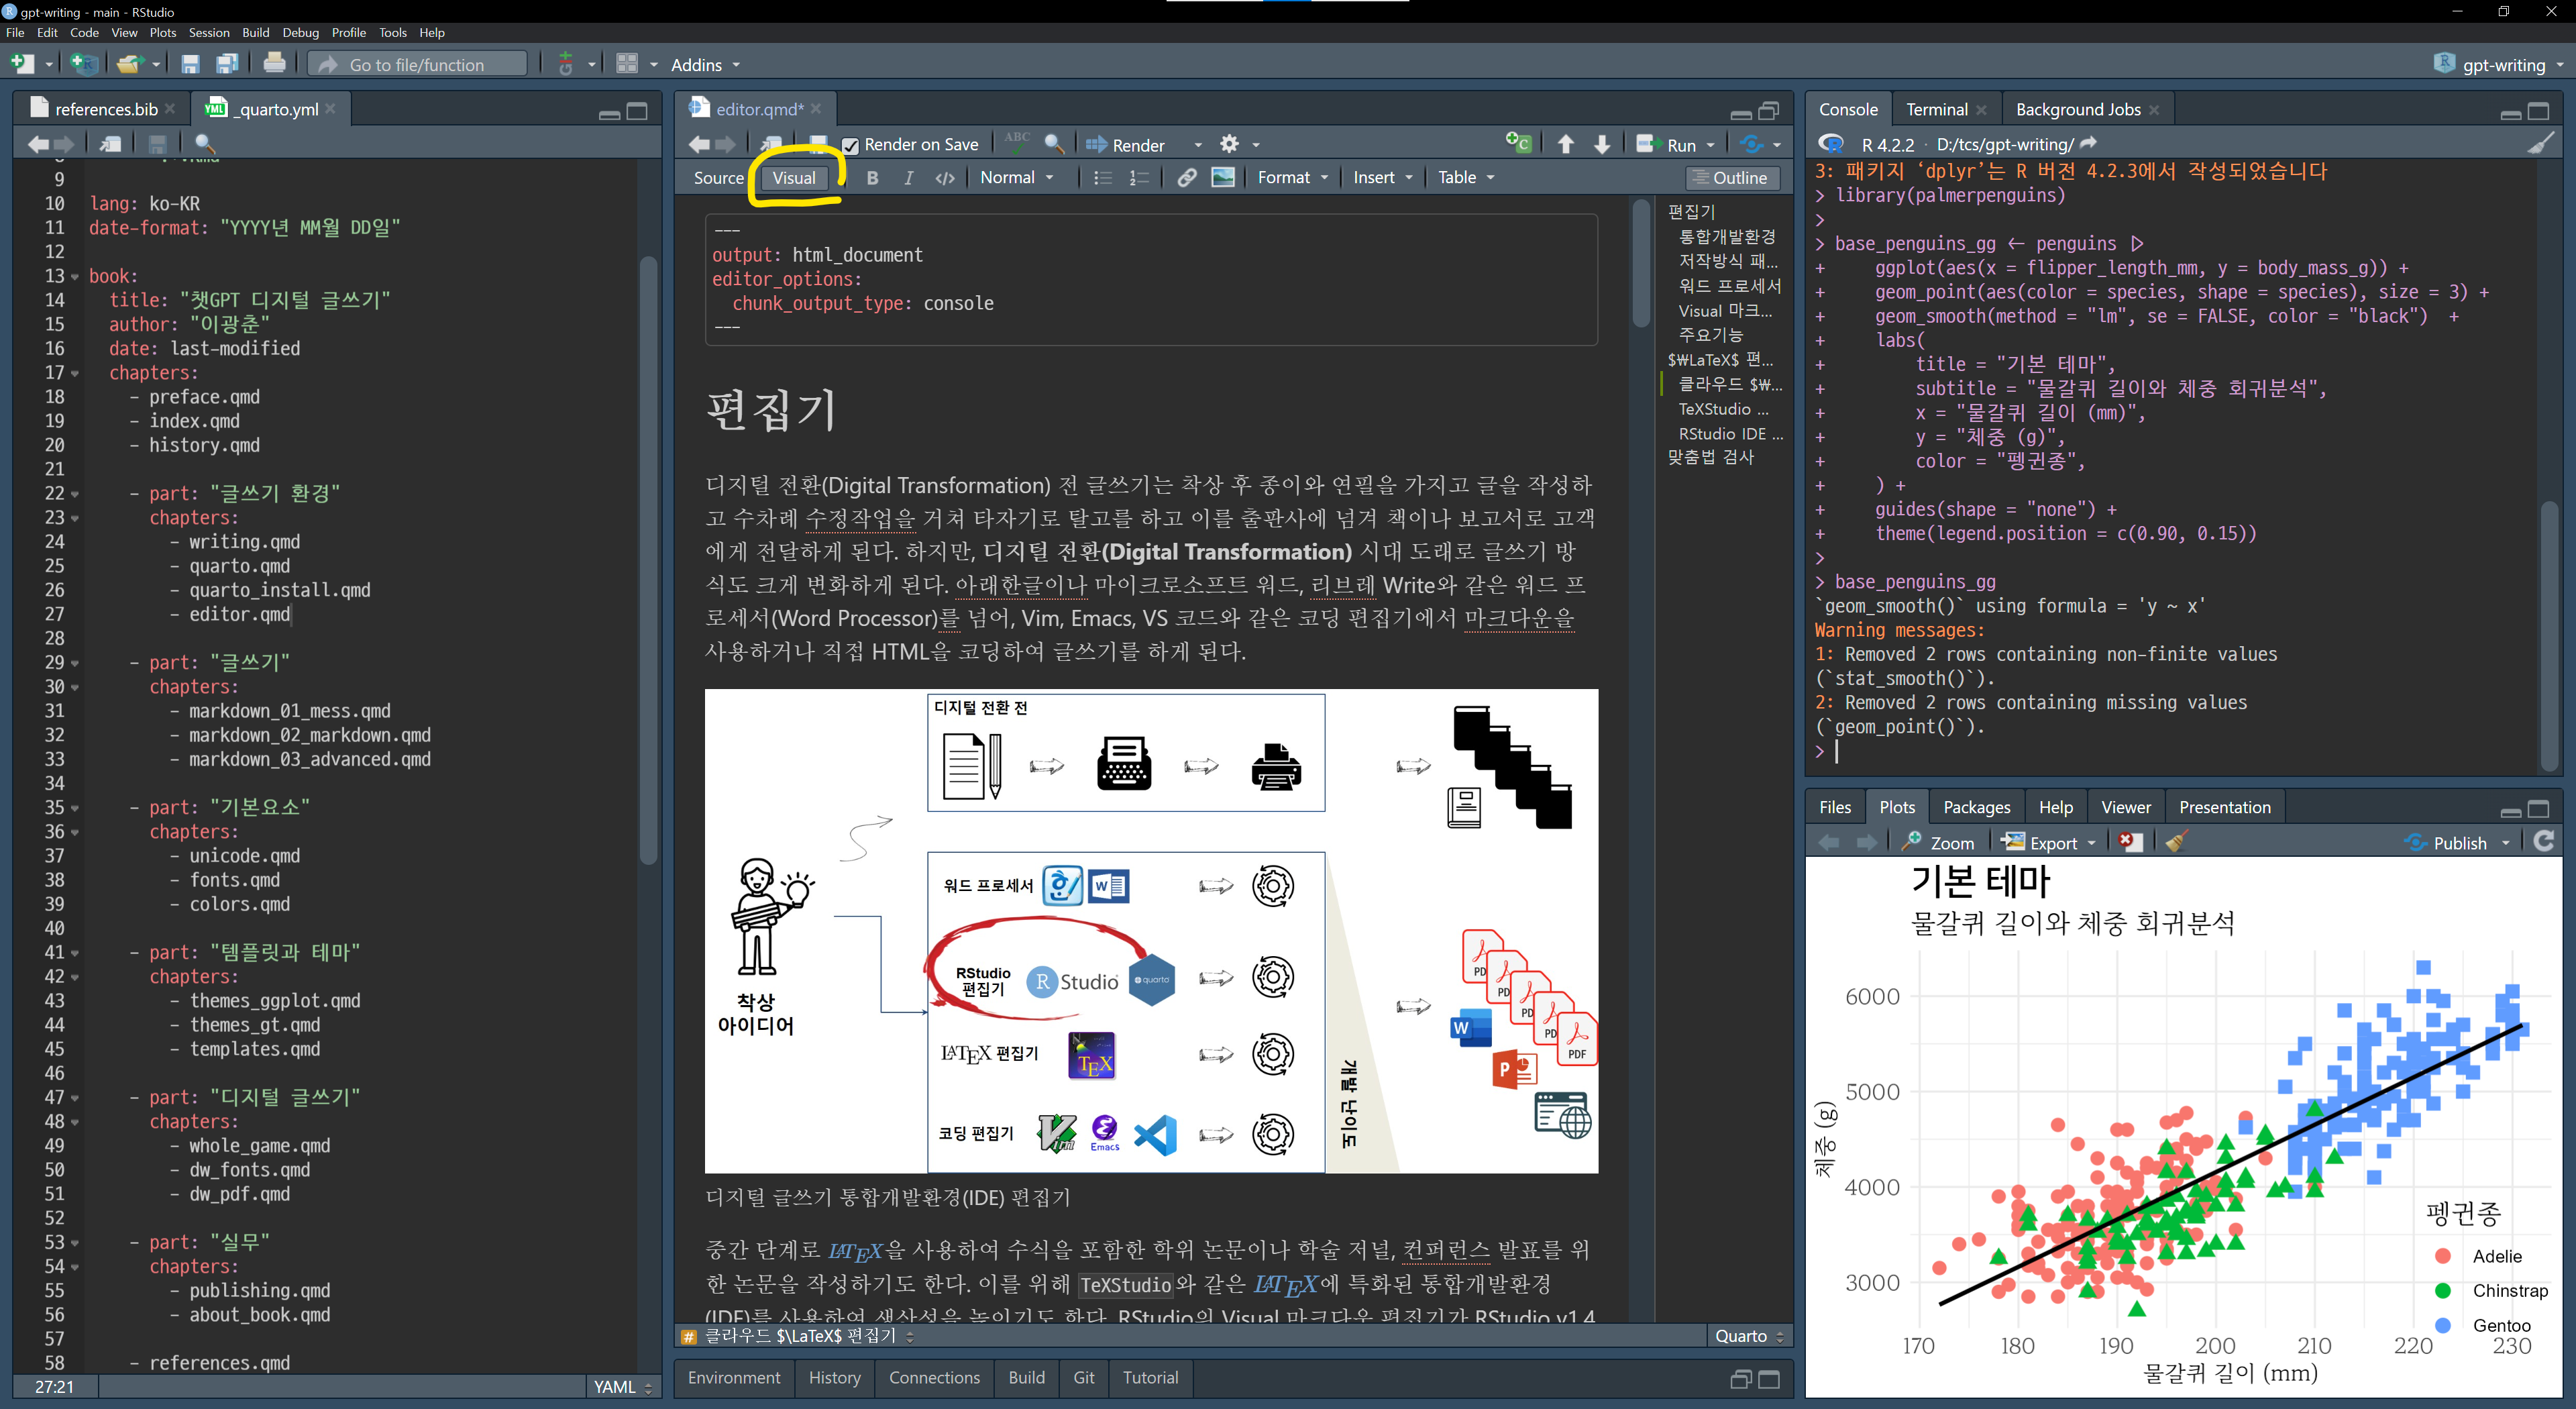
\includegraphics{images/visual-edit-execute-code.png}

}

\caption{RStudio Visual 마크다운 편집기능}

\end{figure}

\hypertarget{uxb9deuxcda4uxbc95-uxac80uxc0ac}{%
\subsection{\texorpdfstring{\protect\hypertarget{spelling-check}{\href{https://statkclee.github.io/comp_document/cd-rstudio-wp.html}{맞춤법
검사}}}{맞춤법 검사}}\label{uxb9deuxcda4uxbc95-uxac80uxc0ac}}

\hypertarget{uxcffcuxd1a0-uxc124uxce58}{%
\section{쿼토 설치}\label{uxcffcuxd1a0-uxc124uxce58}}

\href{https://quarto.org/}{쿼토(Quarto)} 웹사이트에서 Quarto CLI 엔진과
통합개발도구(IDE)를 설치한다. 쿼토 CLI를 지원하는 IDE는 VS Code,
RStudio, Jupyter, VIM/Emacs 와 같은 텍스트 편집기가 포함된다. IDE까지
설치를 했다면 문학적 프로그래밍(literate programming)을 통해 사람이
저작하는 마크다운(Markdown)과 기계가 저작하는 프로그래밍
언어(R/Python/SQL/줄리아/자바스크립트)를 결합한 다양한 문서저작을 시작할
수 있다.

\begin{figure}

{\centering 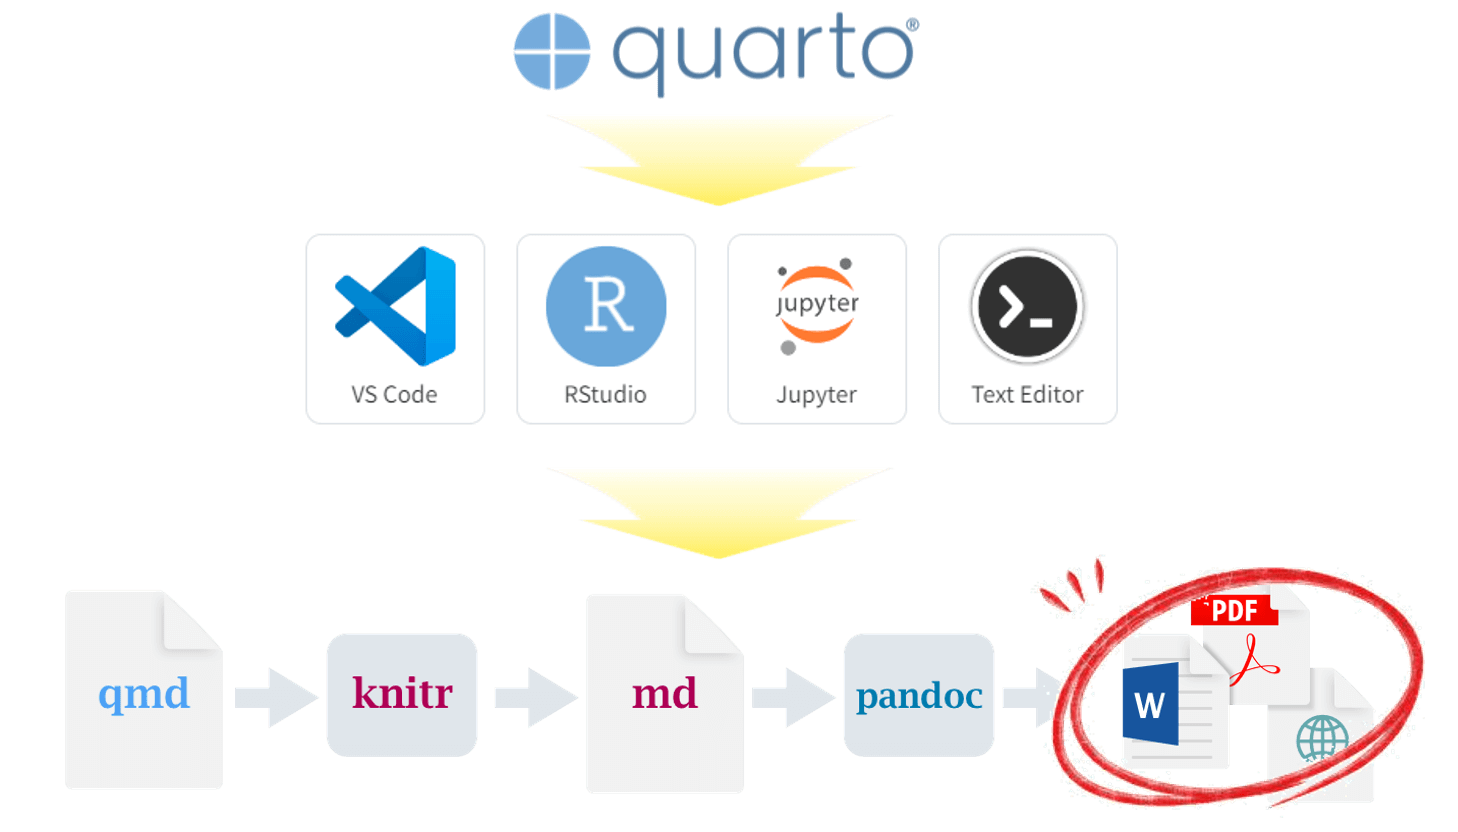
\includegraphics{images/quarto-toolchain.png}

}

\caption{쿼토 도구모음}

\end{figure}

\hypertarget{uxc708uxb3c4uxc6b0-uxc124uxce58}{%
\subsection{윈도우 설치}\label{uxc708uxb3c4uxc6b0-uxc124uxce58}}

\href{https://quarto.org/}{쿼토(Quarto)}를 윈도우 운영체제에 설치하기
위해서는 몇 가지 단계를 거쳐야 한다.

\hypertarget{uxcffcuxd1a0-uxb2e4uxc6b4uxb85cuxb4dc}{%
\subsection{쿼토 다운로드}\label{uxcffcuxd1a0-uxb2e4uxc6b4uxb85cuxb4dc}}

먼저 Quarto 공식 웹사이트에서 윈도우용 설치 파일을 다운로드한다.
웹사이트 \href{https://quarto.org/docs/get-started/}{``Download Quarto
CLI''} 윈도우 버전을 선택하여 다운로드한다.

\begin{figure}

{\centering 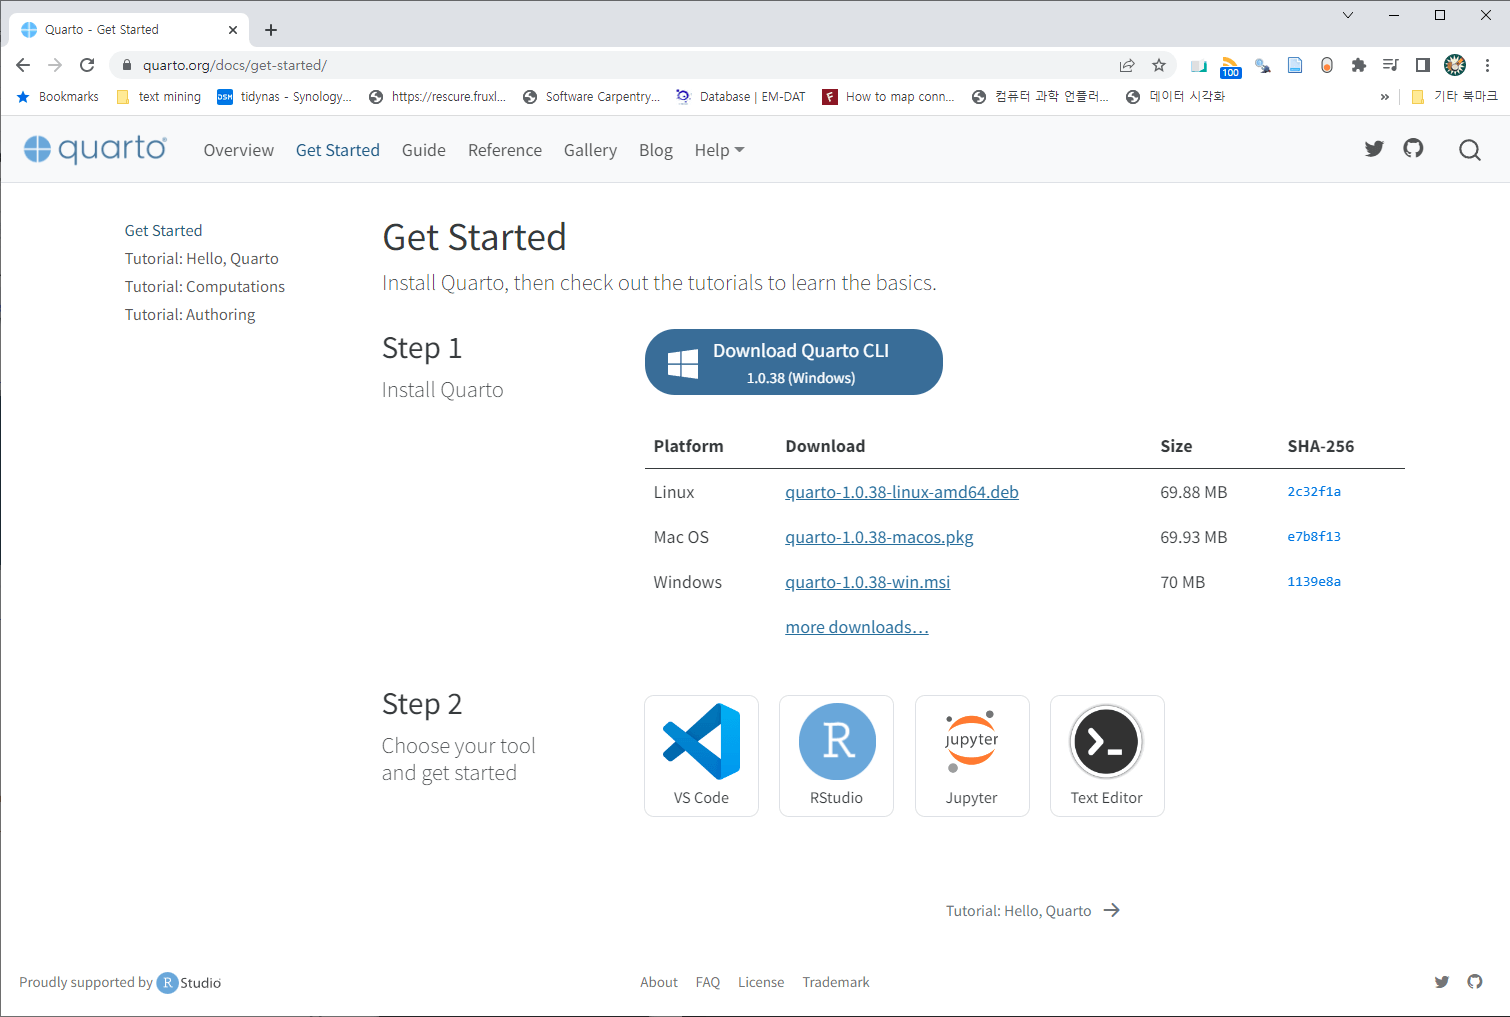
\includegraphics[width=4.16667in,height=\textheight]{images/quarto-download.png}

}

\caption{쿼토 다운로드 화면}

\end{figure}

\hypertarget{uxcffcuxd1a0-uxc124uxce58-1}{%
\subsubsection{쿼토 설치}\label{uxcffcuxd1a0-uxc124uxce58-1}}

다운로드한 파일을 더블클릭 실행하여 설치를 진행한다. 설치 마법사가
나타나면 지시에 따라 설치를 완료하면 된다. 설치가 완료되면 환경 변수에
쿼토 설치 경로를 등록해야 한다. `제어판'을 열고 '시스템과 보안'으로
이동한 다음 '시스템'을 선택한다. '고급 시스템 설정'을 클릭한 후 '환경
변수' 버튼을 누른다. `시스템 변수'에서 'Path' 변수를 찾아 Quarto의 설치
경로를 추가한다. 일반적인 경로는
\texttt{C:\textbackslash{}Users\textbackslash{}\textless{}사용자계정명\textgreater{}\textbackslash{}AppData\textbackslash{}Local\textbackslash{}Programs\textbackslash{}Quarto\textbackslash{}bin}과
같을 수 있다.

\begin{figure}

{\centering 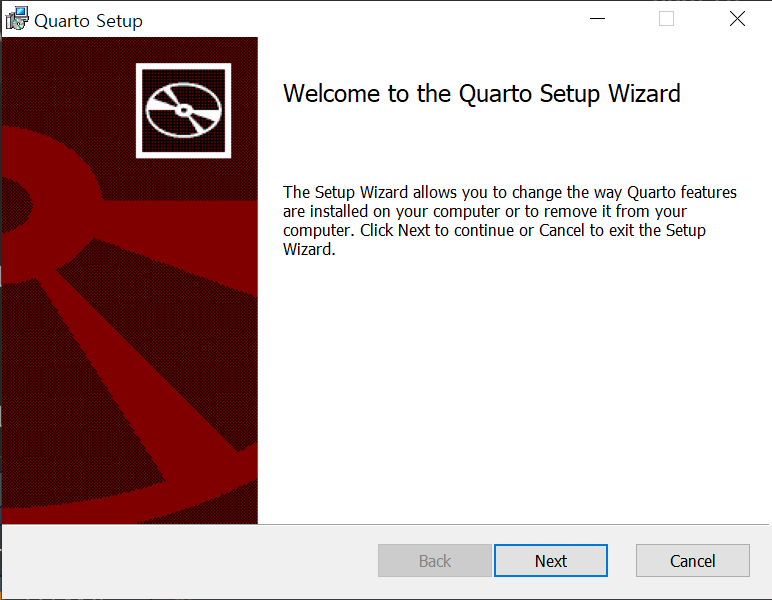
\includegraphics[width=3.64583in,height=\textheight]{images/quarto-install.png}

}

\caption{쿼토 설치완료}

\end{figure}

\hypertarget{uxcffcuxd1a0-cli}{%
\subsection{쿼토 CLI}\label{uxcffcuxd1a0-cli}}

마지막으로 환경 변수 설정이 올바르게 이루어졌는지 확인하기 위해 명령
프롬프트나 터미널을 열어 \texttt{quarto\ -\/-version} 혹은
\texttt{quarto\ -\/-help} 명령을 입력한다. 올바른 버전 번호가 출력되면
설치가 성공적으로 완료된 것이다.

\begin{figure}

{\centering 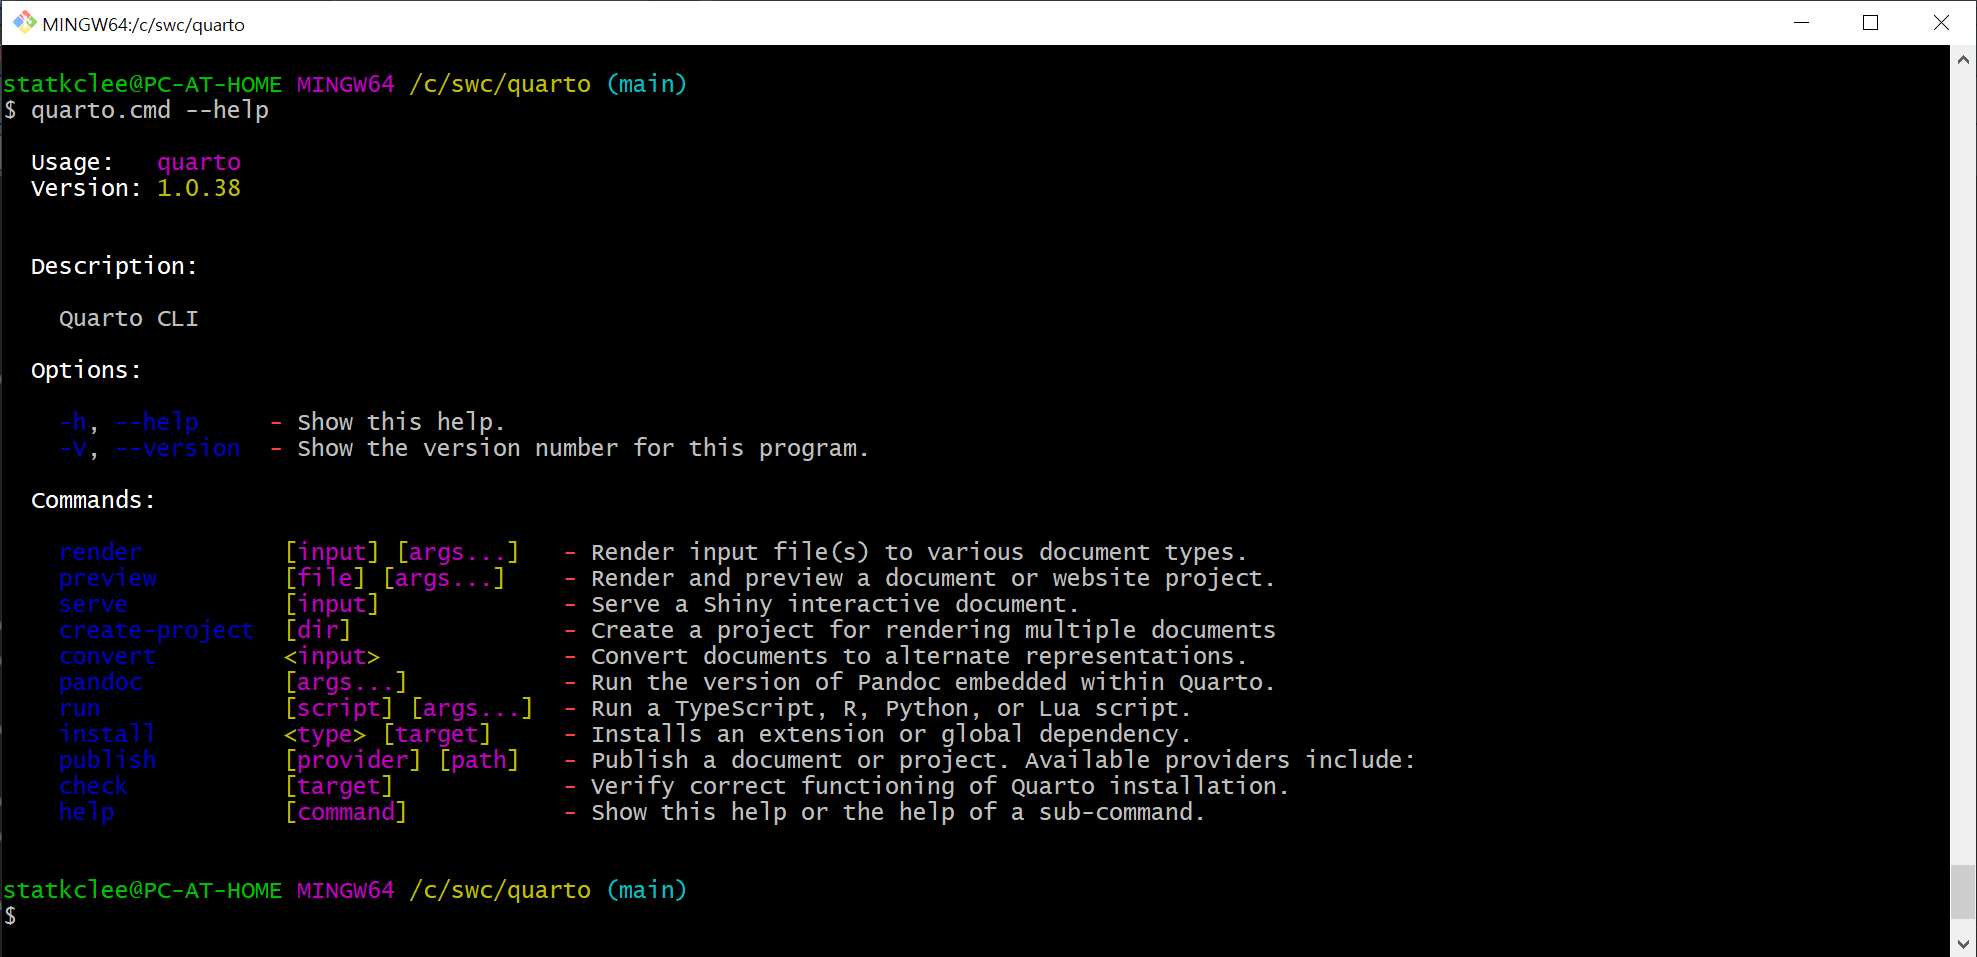
\includegraphics{images/quarto-cli.png}

}

\caption{쿼토 CLI 실행화면}

\end{figure}

\begin{tcolorbox}[enhanced jigsaw, opacityback=0, opacitybacktitle=0.6, colback=white, rightrule=.15mm, coltitle=black, colframe=quarto-callout-tip-color-frame, colbacktitle=quarto-callout-tip-color!10!white, bottomrule=.15mm, bottomtitle=1mm, breakable, title=\textcolor{quarto-callout-tip-color}{\faLightbulb}\hspace{0.5em}{힌트}, titlerule=0mm, leftrule=.75mm, toptitle=1mm, left=2mm, arc=.35mm, toprule=.15mm]

윈도우 시스템의 경우 초기 윈도우에서 쿼토 실행명령이 \texttt{quarto.cmd}
이였으나 \texttt{quarto.exe}도 지원된다. 즉, 제어판 → 환경 변수 설정
\ldots{} 에서
\texttt{"C:\textbackslash{}Users\textbackslash{}사용자명\textbackslash{}AppData\textbackslash{}Local\textbackslash{}Programs\textbackslash{}Quarto\textbackslash{}bin}
디렉토리를 등록한 후 \texttt{quarto} 명령어를 사용한다.

\begin{Shaded}
\begin{Highlighting}[]
\FunctionTok{Sys.which}\NormalTok{(}\StringTok{"quarto"}\NormalTok{)}
\NormalTok{                                                                  quarto }
\StringTok{"C:}\SpecialCharTok{\textbackslash{}\textbackslash{}}\StringTok{Users}\SpecialCharTok{\textbackslash{}\textbackslash{}}\StringTok{사용자명}\SpecialCharTok{\textbackslash{}\textbackslash{}}\StringTok{AppData}\SpecialCharTok{\textbackslash{}\textbackslash{}}\StringTok{Local}\SpecialCharTok{\textbackslash{}\textbackslash{}}\StringTok{Programs}\SpecialCharTok{\textbackslash{}\textbackslash{}}\StringTok{Quarto}\SpecialCharTok{\textbackslash{}\textbackslash{}}\StringTok{bin}\SpecialCharTok{\textbackslash{}\textbackslash{}}\StringTok{quarto.exe"} 
\end{Highlighting}
\end{Shaded}

\end{tcolorbox}

\hypertarget{uxbd80uxc870uxc885uxc0ac}{%
\section{부조종사}\label{uxbd80uxc870uxc885uxc0ac}}

\href{https://github.com/features/copilot}{GitHub 부조종사(Copilot)}를
Rstudio에서 사용하기 위해서는 특별한 버전 Rstudio, 즉
\href{https://dailies.rstudio.com/}{일일 빌드 (Daily Builds)}가 필요하여
각자 운영체제에 맞는 RStudio Desktop 버전을 다운로드한 후 설치한다.

\begin{quote}
\texttt{Tools\ -\textgreater{}\ Global\ Options\ -\textgreater{}\ Copilot\ -\textgreater{}\ Enable\ Github\ Copilot}
\end{quote}

설치가 완료되면 Rstudio를 실행하고 상단 메뉴에서 `Tools'를 선택한 다음
'Global Options'을 클릭하면, 왼쪽 사이드바에서 'Copilot'을 선택하고
'Enable GitHub Copilot' 체크박스를 선택한 다음 'Sign In'을 클릭하고
나타나는 링크에서 인증 코드를 입력한다. 'Authorize Github Copilot
Plugin'을 클릭하여 인증 과정을 완료하면 설정이 완료된다.

\begin{figure}

{\centering 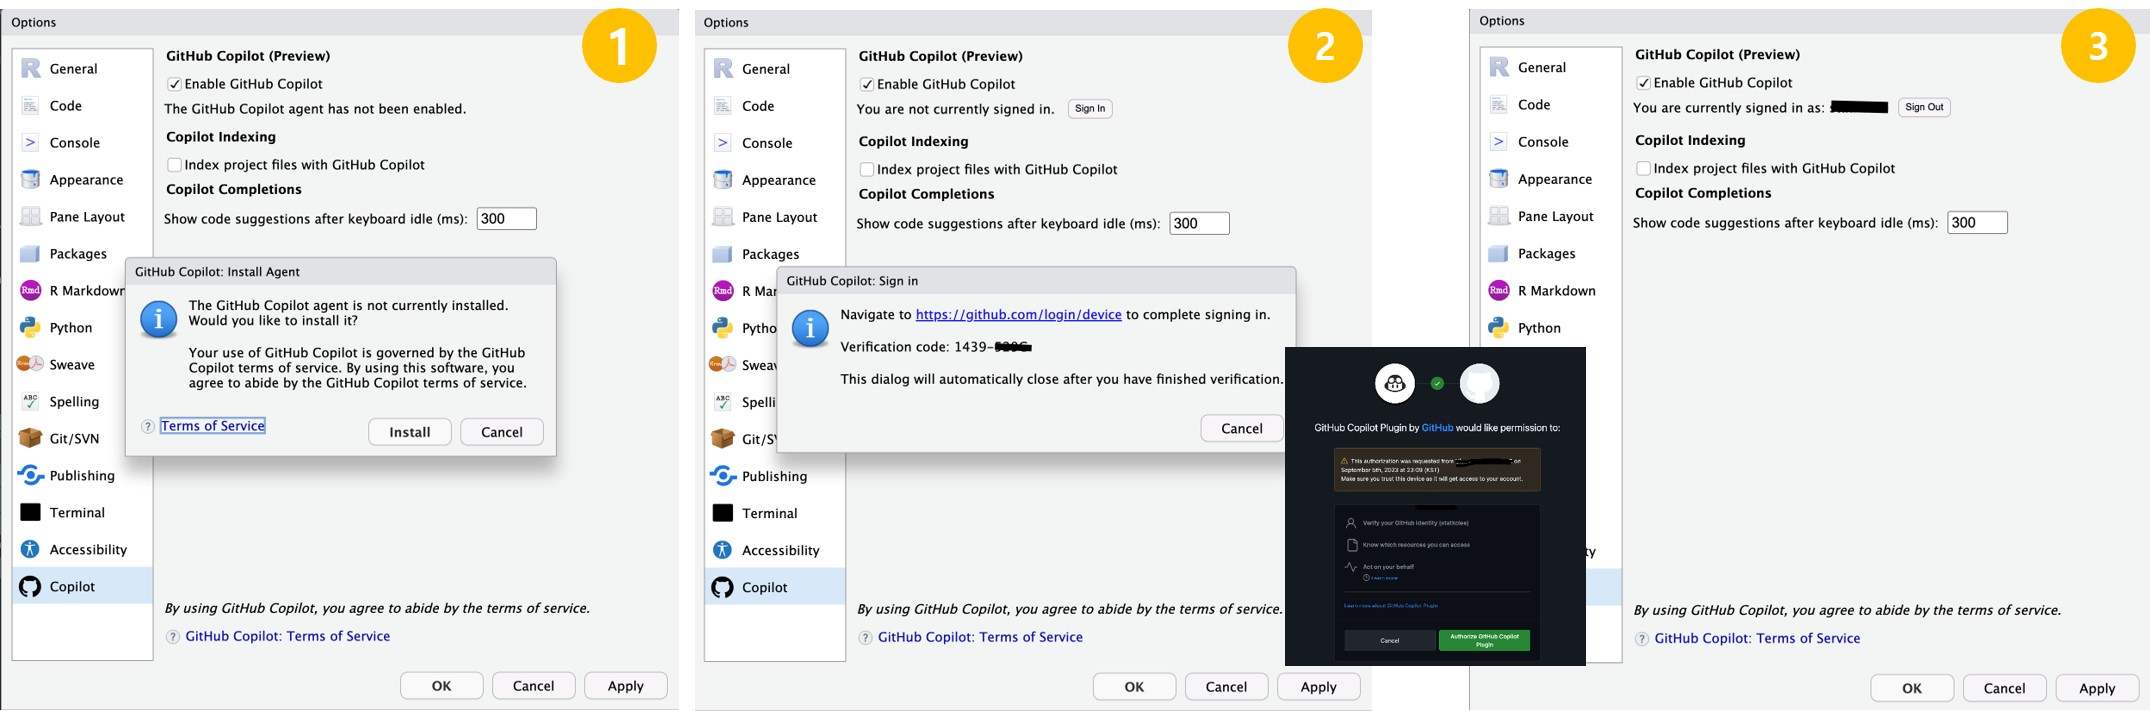
\includegraphics{images/rstudio_copilot.jpg}

}

\caption{GitHub 부주종사 설치과정}

\end{figure}

GitHub Copilot를 Rstudio에서 사용해보면, 작성하려는 코드가 회색으로
예측되어 나타난다. `Tab' 키를 눌러 탭완성(Tab Completion) 기능으로
제시한 코드를 수락하여 개발을 이어간다.

\hypertarget{uxcd9cuxd310-uxd50cuxb7abuxd3fc}{%
\section{출판 플랫폼}\label{uxcd9cuxd310-uxd50cuxb7abuxd3fc}}

데이터 과학 분야에서 산출물을 공유하고 출판하는 것은 매우 중요한 단계로
효과적인 출판과 비용적인 면을 고려하여 최적 플랫폼과 도구를 선정한다.
데이터 과학 분야를 개척한 RStudio IDE로 과거 R 마크다운 산출물을
\href{https://rpubs.com/}{RPubs}에 출판한 경험이 있다면,
\href{https://quartopub.com/}{\texttt{Quarto\ Pub}}은 그와 유사한 경험을
제공한다. 다른 대안으로는 \href{https://netlify.com/}{netlify},
\href{https://github.com/}{GitHub Pages},
\href{https://www.rstudio.com/products/connect/}{RStudio Connect} 등이
있다.

\begin{figure}

{\centering 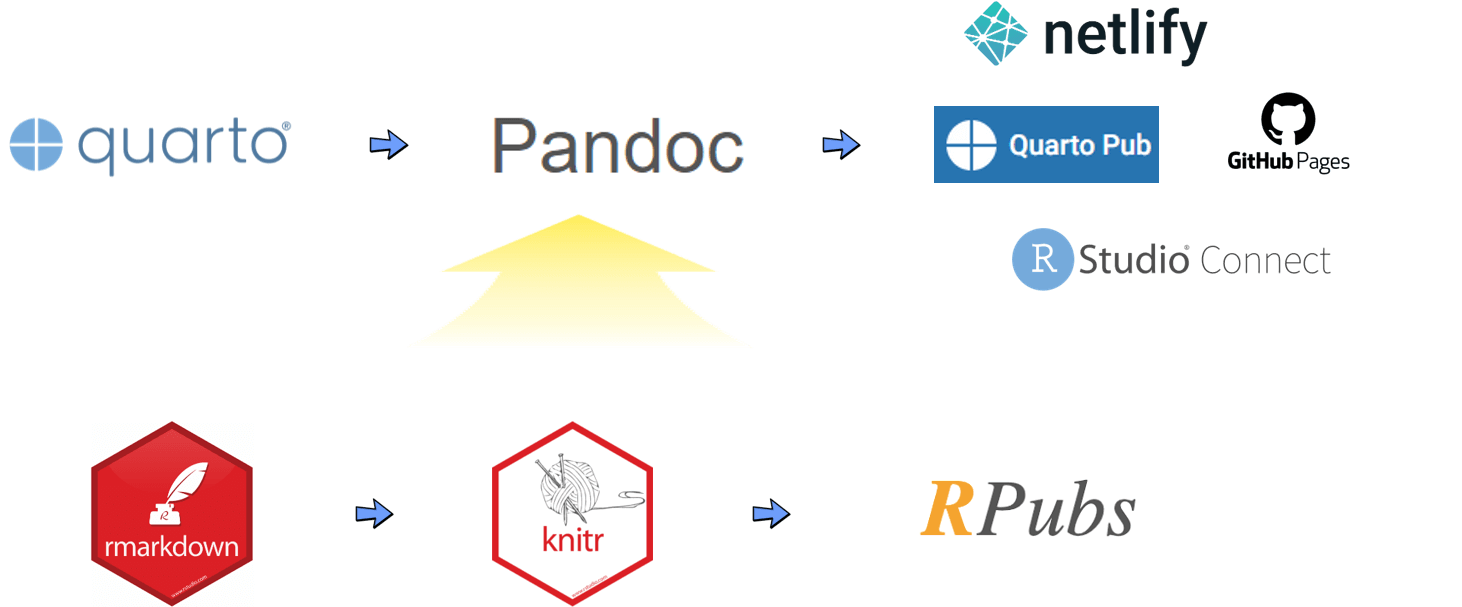
\includegraphics{images/quarto-publishing.png}

}

\caption{쿼토 출판}

\end{figure}

\hypertarget{uxc720uxb2c8uxcf54uxb4dcuxc640-utf-8}{%
\chapter{유니코드와 UTF-8}\label{uxc720uxb2c8uxcf54uxb4dcuxc640-utf-8}}

사람 간의 의사소통은 다양한 기호 체계를 통해 이루어진다. 영어 알파벳,
한글, 한자 등 문자가 의사소통에 사용되는 좋은 예다. 디지털 환경에서
이러한 의사소통을 가능하게 하는 기술적 장치가 바로 문자집합과 문자
인코딩과 디코딩이다.

컴퓨터 시스템은 이진수 바이트를 기본 단위로 사용한다. 바이트는 파일
형태로 묶이거나 네트워크를 통해 전송되어 다른 시스템에 도달한다. 이
데이터가 사람에게 의미 있는 정보로 전달되기 위해서는 인코딩(부호화)과
디코딩(복호화) 과정을 거쳐야 한다.

컴퓨터 시스템은 데이터를 바이트(Byte) 형태로 처리한다. 이 바이트
데이터는 이진수, 즉 010101과 같은 형태로 표현되고, 바이트 데이터를
사람이 읽을 수 있는 문자로 변환하는 최초의 표준이 ASCII(아스키)다.
하지만 ASCII는 256개 문자만을 지원하기 때문에, CJK(중국, 일본, 한국)와
같은 동아시아 문화권에서는 그 한계가 명확하다. 이러한 한계를 해결하기
위해 유니코드(Unicode) 가 도입되었다. 유니코드는 영문자는 물론이고
지구상의 거의 모든 문자와 기호를 디지털로 표현할 수 있는 방법을
제공한다.

\textbf{유니코드(Unicode)}는 글자와 코드가 1:1 매핑되어 있는 단순한
코드표에 불과하고 산업표준으로 일종의 국가 당사자간 약속이다. 한글이
표현된 유니코드 영역도
\href{https://ko.wikipedia.org/wiki/\%EC\%9C\%A0\%EB\%8B\%88\%EC\%BD\%94\%EB\%93\%9C_\%EC\%98\%81\%EC\%97\%AD}{위키백과
유니코드 영역}에서 찾을 수 있다.

\begin{figure}

{\centering 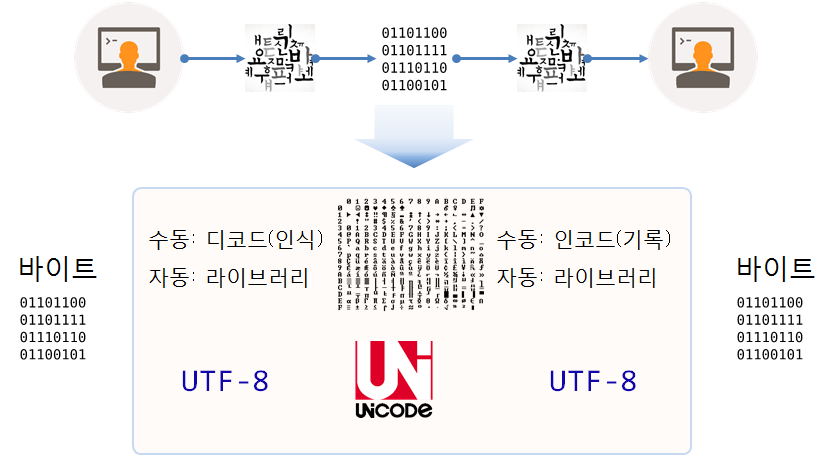
\includegraphics{images/auth-unicode-utf-8.png}

}

\caption{유니코드와 UTF-8}

\end{figure}

\begin{tcolorbox}[enhanced jigsaw, opacityback=0, opacitybacktitle=0.6, colback=white, rightrule=.15mm, coltitle=black, colframe=quarto-callout-note-color-frame, colbacktitle=quarto-callout-note-color!10!white, bottomrule=.15mm, bottomtitle=1mm, breakable, title=\textcolor{quarto-callout-note-color}{\faInfo}\hspace{0.5em}{인코딩 (Encoding)}, titlerule=0mm, leftrule=.75mm, toptitle=1mm, left=2mm, arc=.35mm, toprule=.15mm]

\textbf{문자 인코딩(character encoding)} 줄여서 인코딩은 사용자가 입력한
문자나 기호들을 컴퓨터가 이용할 수 있는 신호로 만드는 것을 말한다. 넓은
의미의 컴퓨터는 이러한 신호를 입력받고 처리하는 기계를 뜻하며, 신호 처리
시스템을 통해 이렇게 처리된 정보를 사용자가 이해할 수 있게 된다.

\begin{quote}
All text has a character encoding.
\end{quote}

\end{tcolorbox}

\hypertarget{uxc778uxcf54uxb529-uxbb38uxc81c}{%
\section{인코딩 문제}\label{uxc778uxcf54uxb529-uxbb38uxc81c}}

문자 인코딩은 컴퓨터가 텍스트를 바이트로 변환하거나 바이트를 텍스트로
변환하는 방법이다. 인코딩 과정에서는 다양한 문제가 발생할 수 있고, 그 중
세 가지 문제가 많이 알려져있다. 첫번째는 '두부(Tofu)'라 불리는 상황으로,
컴퓨터가 어떤 문자를 표현해야 할지 알지만, 화면에 어떻게 출력해야 할지
모르기 때문에 빈 사각형 상자로 표시된다. 두번째는 '문자깨짐(Mojibake,
文字化け)'이다. 특히 일본어에서 자주 발생하며, 한 인코딩 방식으로 작성된
텍스트가 다른 인코딩 방식으로 해석될 때 문자가 깨지는 현상을 의미한다.
세번째는 '의문부호(Question Marks)'로, 특정 문자가 다른 문자로 변환될 때
발생된다. 문자집합과 인코딩 궁합이 맞지 않을 때 발생하며, 데이터 손실과
오류도 야기된다.

\begin{figure}

{\centering 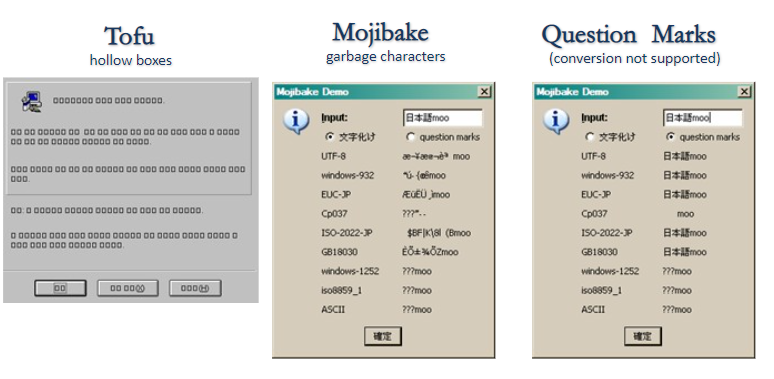
\includegraphics{images/common-encoding-problem.png}

}

\caption{세가지 인코딩 문제}

\end{figure}

\hypertarget{uxbb38uxc790-uxc9d1uxd569}{%
\section{문자 집합}\label{uxbb38uxc790-uxc9d1uxd569}}

\hypertarget{uxc544uxc2a4uxd0a4-uxcf54uxb4dc}{%
\subsection{아스키 코드}\label{uxc544uxc2a4uxd0a4-uxcf54uxb4dc}}

디지털 글쓰기는 내용과 상관없이 결국 텍스트로 표현되고, 텍스트는 단지
문자다. 하지만, 컴퓨터가 문자 하나를 어떻게 표현할까?

1960년대 미국식 영문자를 컴퓨터로 표현하는 해결책은 간단했다 - 알파벳
26개(대문자, 소문자), 숫자 10, 구두점 몇개, 그리고 전신을 보내던 시절에
제어를 위해 사용된 몇개 특수 문자(``새줄로 이동'', ``본문 시작'',
``개행'', ``경고음'', 등). 모두 합쳐도 128개보다 적어서, 아스키(ASCII)
위원회가 문자마다 7비트( \(2^7\) = 128)를 사용하는 인코딩으로
표준화했다. \footnote{미국정보교환표준부호(American Standard Code for
  Information Interchange, ASCII)는 영문 알파벳을 사용하는 대표적인 문자
  인코딩으로 컴퓨터와 통신 장비를 비롯한 문자를 사용하는 많은 장치에서
  사용되며, 대부분의 문자 인코딩이 아스키에 기초하고 있다.}

\begin{figure}

{\centering 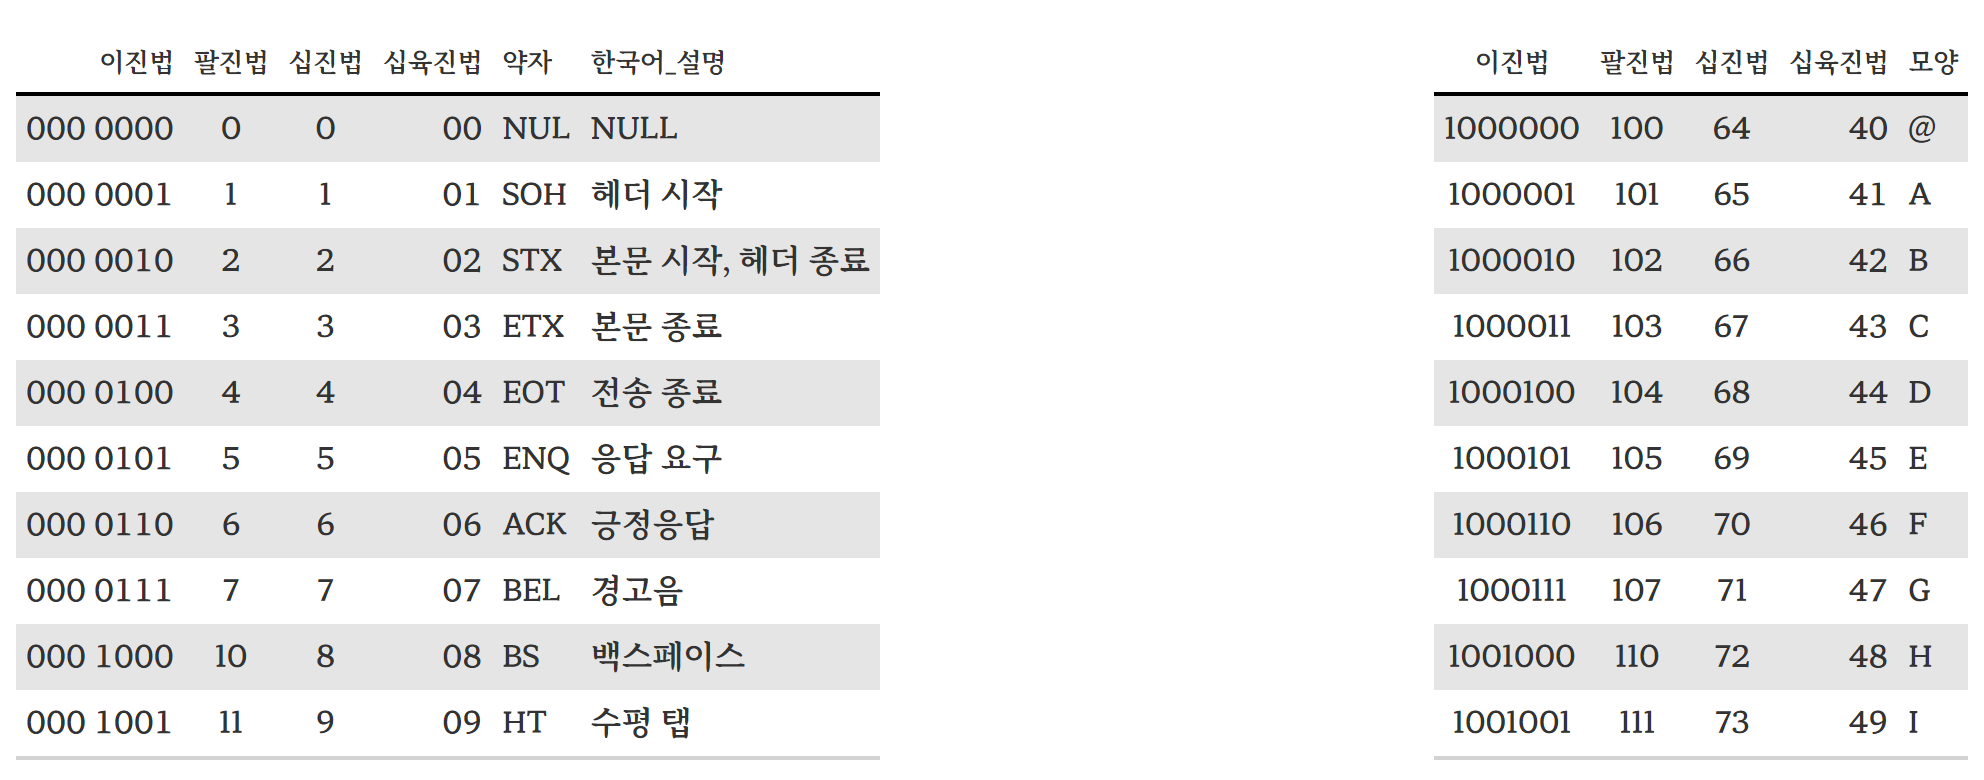
\includegraphics{images/ascii_gt.png}

}

\caption{\label{fig-ascii}제어문자와 출력가능한 아스키 문자표 알파벳
예시}

\end{figure}

그림~\ref{fig-ascii} 에 아스키 문자표에 제어문자 10개와 출력가능 아스키
문자표 중 영문 대문자 A-I까지 10개를 뽑아 사례로 보여주고 있다. 즉,
문자표는 어떤 문자가 어떤 숫자에 해당하는지를 정의하고 있다.

\hypertarget{ascii-extension}{%
\subsection{확장 아스키}\label{ascii-extension}}

아스키(ASCII) 방식으로 숫자 \texttt{2}, 문자 \texttt{q}, 혹은 곡절
악센트 \texttt{\^{}} 를 표현하는데 충분하다. 하지만, 투르크어족 추바시어
\texttt{ĕ}, 그리스 문자 \texttt{β}, 러시아 키릴문자 \texttt{Я} 는 어떻게
저장하고 표현해야 할까? 7-비트를 사용하면 0 에서 127까지 숫자를 부여할
수 있지만, 8-비트(즉, 1 바이트)를 사용하게 되면 255까지 표현할 수 있다.
그렇다면, ASCII 표준을 확장해서 추가되는 128개 숫자에 대해 추가로 문자를
표현할 수 있게 된다.

\begin{itemize}
\tightlist
\item
  아스키: 0\ldots127
\item
  확장된 아스키: 128\ldots255
\end{itemize}

불행하게도, 영어문자를 사용하지 않는 세계 곳곳에서 많은 사람들이 시도를
했지만, 방식도 다르고, 호환이 되지 않는 방식으로 작업이 되어, 결과는
엉망진창이 되었다. 예를 들어, 실제 텍스트가 불가리아어로 인코딩되었는데
스페인어 규칙을 사용해서 인코딩한 것으로 프로그램이 간주하고 처리될 경우
결과는 무의미한 횡설수설 값이 출력된다. 이와는 별도로 한중일(CJK)
동아시아 국가들을 비롯한 많은 국가들이 256개 이상 기호를 사용한다.
왜냐하면 8-비트로 특히 동아시아 국가 문자를 표현하는데 부족하기
때문이다.

\hypertarget{uxd55cuxae00-uxc644uxc131uxd615uxacfc-uxc870uxd569uxd615}{%
\subsection{한글 완성형과
조합형}\label{uxd55cuxae00-uxc644uxc131uxd615uxacfc-uxc870uxd569uxd615}}

1980년대부터 컴퓨터를 사용하신 분이면 완성형과 조합형의 표준화 전쟁을
지켜봤을 것이고, 그 이면에는 한글 워드프로세서에 대한 주도권 쟁탈전이
있었던 것을 기억할 것이다. 결국 완성형과 조합형을 모두 포용하는 것으로
마무리 되었지만, 여기서 끝난게 끝난 것이 아니다. 유닉스 계열에서
\texttt{KSC5601}을 표준으로 받아들인 \texttt{EUC-KR}과 90년대와
2000년대를 호령한 마이크로소프트 \texttt{CP949} 가 있었다. 결국 대한민국
정부에서 주도한 표준화 전쟁은 유닉스/리눅스, 마이크로소프트 모두를
녹여내는 것으로 마무리 되었고, 웹과 모바일 시대는 유니코드로 넘어가서
\texttt{KSC5601}이 유니코드의 원소로 들어가는 것으로 마무리 되었다.

이제 신경쓸 것은 인코딩 \ldots{} \texttt{utf-8} 만 신경쓰면 된다. 그리고
남은 디지털 레거시 유산을 잘 처리하면 된다.

\begin{tcolorbox}[enhanced jigsaw, opacityback=0, opacitybacktitle=0.6, colback=white, rightrule=.15mm, coltitle=black, colframe=quarto-callout-note-color-frame, colbacktitle=quarto-callout-note-color!10!white, bottomrule=.15mm, bottomtitle=1mm, breakable, title=\textcolor{quarto-callout-note-color}{\faInfo}\hspace{0.5em}{유닉스/리눅스(EUC-KR), 윈도우(CP949)}, titlerule=0mm, leftrule=.75mm, toptitle=1mm, left=2mm, arc=.35mm, toprule=.15mm]

\texttt{EUC-KR}, \texttt{CP949} 모두 2바이트 한글을 표현하는 방식으로
동일점이 있지만, \texttt{EUC-KR} 방식은 KSC5601-87 완성형을 초기
사용하였으나, KSC5601-92 조합형도 사용할 수 있도록 확장되었다.
\texttt{CP949}는 확장 완성형으로도 불리며 \texttt{EUC-KR}에서 표현할 수
없는 한글글자 8,822자를 추가한 것으로 마이크로소프트 코드페이지(Code
Page) 949를 사용하면서 일반화되었다.

\end{tcolorbox}

\hypertarget{ascii-unicode}{%
\subsection{유니코드}\label{ascii-unicode}}

1990년대 나타나기 시작한 해결책을 \textbf{유니코드(Unicode)} 라고
부른다. 예를 들어, 영어 A 대문자는 1 바이트, 한글 가는 3 바이트다.
유니코드는 정수값을 서로 다른 수만개 문자와 기호를 표현하는데 정의한다.
'A'는 \texttt{U+0041}, '가'는 \texttt{U+AC00}과 같이 고유한 코드
포인트를 가진다. 하지만, 파일에 혹은 메모리에 문자열로 정수값을 저장하는
방식을 정의하지는 않는다.

각 문자마다 8-비트를 사용하던 방식에서 32-비트 정수를 사용하는 방식으로
전환하면 되지만, 영어, 에스토니아어, 브라질 포르투칼어 같은 알파벳
언어권에는 상당한 공간 낭비가 발생된다. 접근 속도가 중요한 경우 메모리에
문자당 32 비트를 종종 사용한다. 하지만, 파일에 데이터를 저장하거나
인터넷을 통해 전송하는 경우 대부분의 프로그램과 프로그래머는 이와는 다른
방식을 사용한다.

다른 방식은 (거의) 항상 \textbf{UTF-8} 으로 불리는 인코딩으로, 문자 마다
가변 바이트를 사용한다. 하위 호환성을 위해, 첫 128개 문자(즉, 구 아스키
문자집합)는 바이트 1개에 저장된다. 다음 1920개 문자는 바이트 2개를
사용해서 저장된다. 다음 61,000은 바이트 3개를 사용해서 저장해 나간다.

궁금하면, 동작 방식이 다음 표에 나타나 있다. ``전통적'' 문자열은
문자마다 1 바이트를 사용한다. 반대로, ``유니코드'' 문자열은 문자마다
충분한 메모리를 사용해서 어떤 텍스트 유형이든 저장한다. R, 파이썬 3.x
에서 모든 문자열은 유니코드다. 엄청난 바이트를 읽어오거나 저장하여
내보내려고 할때, 인코딩을 지정하는 것은 엄청난 고통이다.

유니코드 문자열은 여는 인용부호 앞에 소문자 \texttt{U}를 붙여 표시한다.
유니코드 문자열을 바이트 문자열로 전환하려면, 인코딩을 명세해야만 된다.
항상 UTF-8을 사용해야만 되고, 그밖의 인코딩을 사용하는 경우 매우, 매우
특별히 좋은 사유가 있어야만 된다. 특별한 인코딩을 사용하는 경우 두번
생각해 보라.

\begin{figure}

{\centering 
\includegraphics{images/ascii_evolution.jpg}

}

\caption{아스키에서 유니코드로 진화과정}

\end{figure}

컴퓨터가 처음 등장할 때 미국 영어권 중심 아스키가 아니고 4바이트 전세계
모든 글자를 표현할 수 있는 유니코드가 사용되었다면 한글을 컴퓨터에
표현하기 위한 지금과 같은 번거로움은 없었을 것이다. 돌이켜보면 초기
컴퓨터가 저장용량 한계로 인해 유니코드가 표준으로 자리를 잡더라도
실용적인 이유로 인해서 한글을 컴퓨터에 표현하기 위한 다른 대안이
제시됐을 것도 분명해 보인다. 초창기 영어권을 중심으로 아스키 표준이
정립되어 현재까지 내려오고, 유니코드와 UTF-8 인코딩이 사실상 표준으로
자리잡았으며, 그 사이 유닉스/리눅스 EUC-KR, 윈도우즈 CP949가 빈틈을
한동안 매우면서 역할을 담당했다.

\begin{longtable}[]{@{}
  >{\centering\arraybackslash}p{(\columnwidth - 8\tabcolsep) * \real{0.2000}}
  >{\centering\arraybackslash}p{(\columnwidth - 8\tabcolsep) * \real{0.2000}}
  >{\centering\arraybackslash}p{(\columnwidth - 8\tabcolsep) * \real{0.2000}}
  >{\centering\arraybackslash}p{(\columnwidth - 8\tabcolsep) * \real{0.2000}}
  >{\centering\arraybackslash}p{(\columnwidth - 8\tabcolsep) * \real{0.2000}}@{}}
\toprule\noalign{}
\begin{minipage}[b]{\linewidth}\centering
항목
\end{minipage} & \begin{minipage}[b]{\linewidth}\centering
ASCII (1963)
\end{minipage} & \begin{minipage}[b]{\linewidth}\centering
EUC-KR (1980s)
\end{minipage} & \begin{minipage}[b]{\linewidth}\centering
CP949 (1990s)
\end{minipage} & \begin{minipage}[b]{\linewidth}\centering
Unicode (1991)
\end{minipage} \\
\midrule\noalign{}
\endhead
\bottomrule\noalign{}
\endlastfoot
범위 & 128개의 문자 & 2,350개의 한글 문자 등 & 약 11,172개의 완성형 한글
문자 등 & 143,859개의 문자 (버전 13.0 기준) \\
비트 수 & 7비트 & 8\textasciitilde16비트 & 8\textasciitilde16비트 &
다양한 인코딩 방식 (UTF-8, UTF-16, UTF-32 등) \\
표준 & ANSI, ISO/IEC 646 & KS X 2901 & 마이크로소프트 & ISO/IEC 10646 \\
플랫폼 & 다양한 시스템 & UNIX 계열, 일부 Windows & Windows 계열 & 다양한
플랫폼 \\
문자 집합 & 영문 알파벳, 숫자, 특수 문자 & 한글, 영문 알파벳, 숫자, 특수
문자 & 한글, 한자, 영문 알파벳, 숫자, 특수 문자 & 전 세계 언어, 특수
문자, 이모티콘 등 \\
확장성 & 확장 불가능 & 한정적 & 더 많은 문자 지원 & 높은 확장성 \\
국제성 & 영어 중심 & 한국어 중심 & 한국어 중심 & 다국어 지원 \\
유니코드 호환 & 호환 가능 (U+0000 \textasciitilde{} U+007F) & 호환 불가,
변환 필요 & 유니코드와 상호 변환 가능 & 자체가 표준 \\
\end{longtable}

\hypertarget{utf-8}{%
\section{UTF-8}\label{utf-8}}

UTF-8(Universal Coded Character Set + Transformation Format -- 8-bit의
약자)은 유니코드 중에서 가장 널리 쓰이는 인코딩으로, 유니코드를 위한
가변 길이 문자 인코딩 방식 중 하나로 켄 톰프슨과 롭 파이크가 제작했다.

UTF-8 인코딩의 가장 큰 장점은 아스키(ASCII), 라틴-1(ISO-8859-1)과
호환되어, 문서를 처리하는 경우 아스키, 라틴-1 문서를 변환 없이 그대로
처리할 수 있고 영어를 비롯한 라틴계열 문서로 저장할 때 용량이 매우 작다.
이러한 이유로 많은 오픈소스 소프트웨어와 데이터를 생산하는 미국을 비롯한
유럽언어권에서 UTF-8이 많이 사용되고 있지만, 한글은 한 글자당 3바이트
용량을 차지한다.

\hypertarget{uxc6f9-uxd45cuxc900-uxc778uxcf54uxb529}{%
\subsection{웹 표준
인코딩}\label{uxc6f9-uxd45cuxc900-uxc778uxcf54uxb529}}

스마트폰의 대중화에 따라 더이상 윈도우 운영체제에서 사용되는 문자체계가
더이상 표준이 되지 못하고 여러 문제점을 야기함에 따라 \textbf{유니코드 +
UTF-8} 체제가 대세로 자리잡고 있는 것이 확연히 나타나고 있다.

2010년 구글에서
\href{https://googleblog.blogspot.com/2010/01/unicode-nearing-50-of-web.html}{발표}한
자료에 의하면 2010년 UTF-8 인코딩이 웹에서 주류로 부상하기 시작한 것이
확인되었다. \autocite{unicode2010} 웹기반 플롯 디지털 도구를 활용하여
그래프(\href{https://apps.automeris.io/wpd/}{WebPlotDigitizer})에서
데이터를 추출하여 시각화면 유사한 결과를 시각적으로 표현할 수 있다.
2010년 이후 웹에서 가장 점유율이 높은 인코딩 방식은 UTF-8으로 W3Tech
웹기술조사(Web Technology Surveys)를 통해 확인을 할 수 있다. 여기서
주목할 점은, 프랑스어, 독일어, 스페인어와 같은 서유럽 언어의 문자와 기호
표현하는 ISO-8859-1 인코딩, 종종 ``Latin-1''으로 불리는 8비트 문자
인코딩이 현저히 줄고 있다는 점이다.

\begin{figure}

{\centering 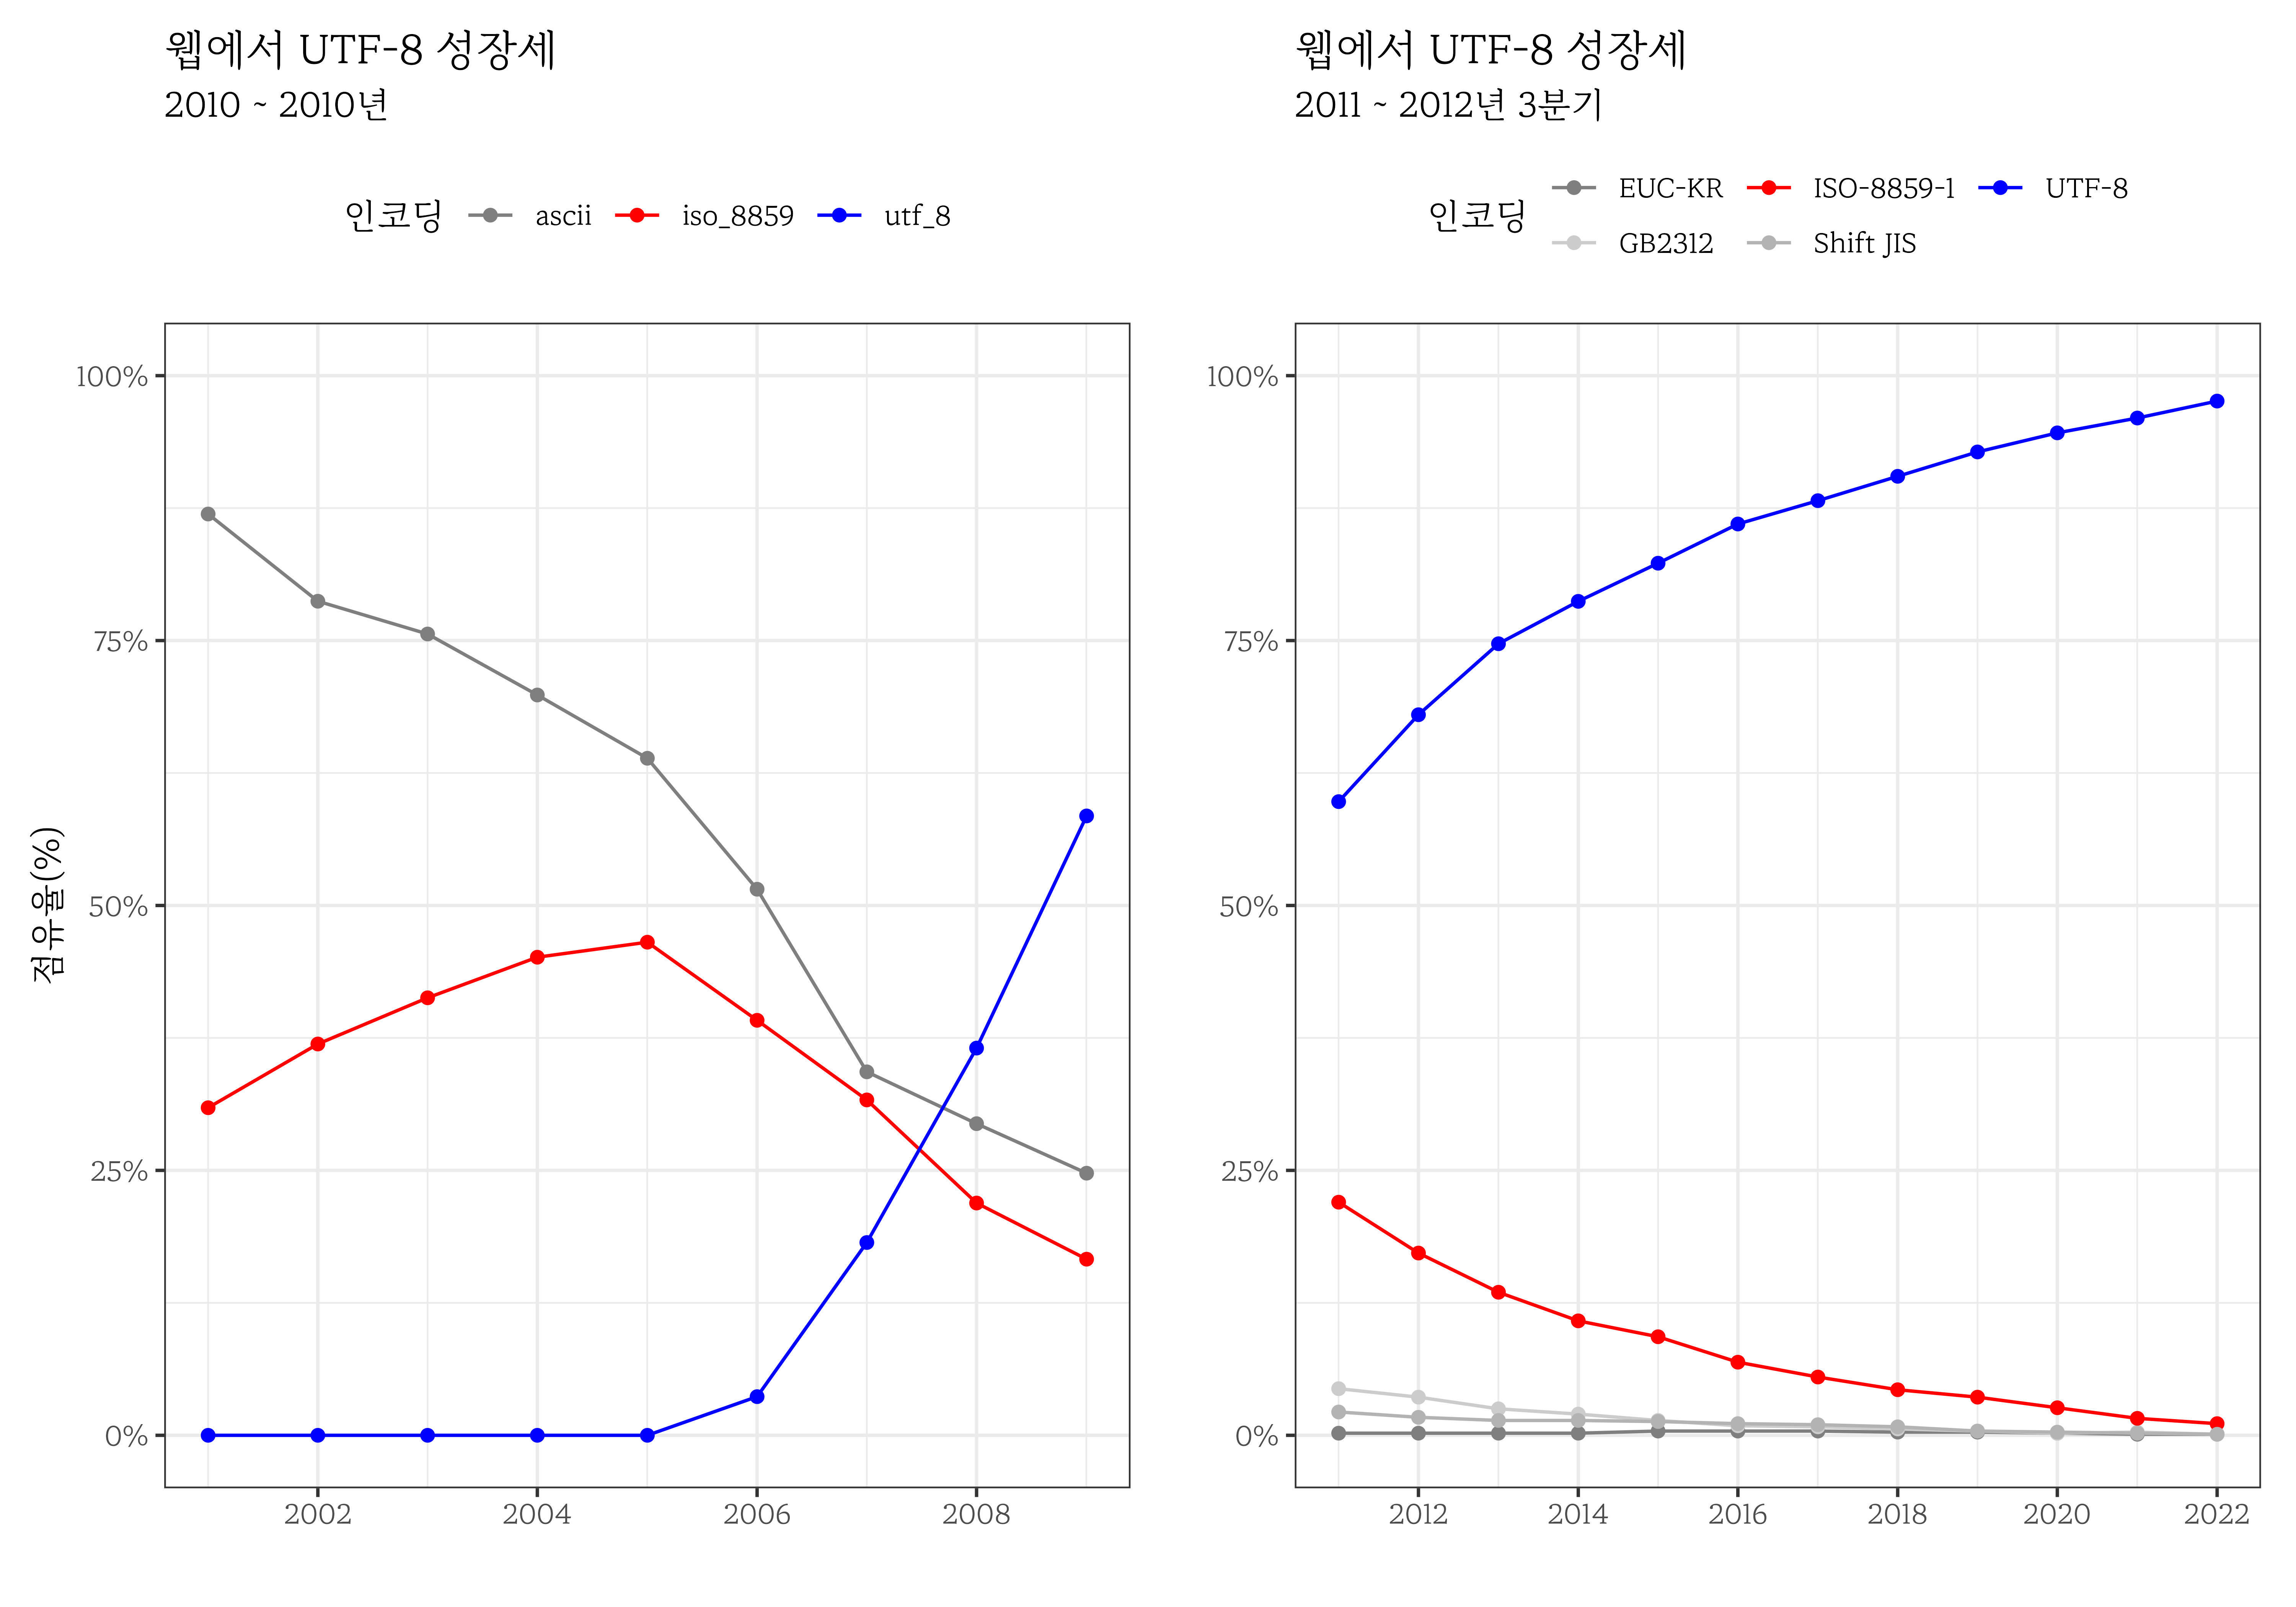
\includegraphics{images/encoding_utf_gg.jpg}

}

\caption{2010 \textasciitilde{} 2012 웹에서 UTF-8 성장세}

\end{figure}

\hypertarget{uxd14duxc2a4uxd2b8-uxd45cuxd604}{%
\section{텍스트 표현}\label{uxd14duxc2a4uxd2b8-uxd45cuxd604}}

1940년대, 1950년대 펀치카드 기술로 정의된 첫번째 방식이 \textbf{고정폭
레코드(fixed-width records)} 를 사용하는 것으로, 각 줄마다 동일한
고정길이를 갖는다. 예를 들어, 다음 일본 전통 단시 하이쿠(haiku)를
컴퓨터로 아래와 같이 레코드 3개로 배열했다. (점 문자는 ``사용되지
않음''을 의미) 이런 방식은 여전히 데이터베이스에도 사용되고 있다.

\begin{quote}
\textbf{일본 전통 단시 하이쿠 예시}

\begin{Shaded}
\begin{Highlighting}[]
\NormalTok{A crash reduces}
\NormalTok{your expensive computer}
\NormalTok{to a simple stone.}
\end{Highlighting}
\end{Shaded}
\end{quote}

\begin{figure}

{\centering 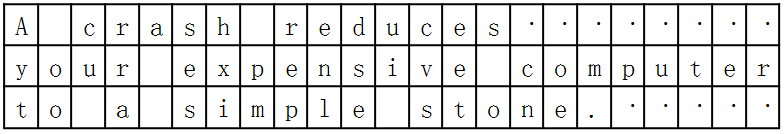
\includegraphics{images/regex-encoding-fixed-width.png}

}

\caption{고정길이 일본 전통 하이쿠 표현}

\end{figure}

이런 표기법은 N번째 행 앞으로 뒤로 건너뛰기 쉬운데 이유는 각 행이 동일한
크기를 갖기 때문이다. 하지만, 공간을 낭비하는 약점이 있고, 행마다 얼마나
긴 최대 길이를 갖느냐에 관계없이, 궁극적으로 더 긴 길이를 갖는 행을
기준으로 처리해야만 된다.

시간이 흐름에 따라 개발자 대부분은 다른 표현법으로 전환했다. 전환된
표현법에 따르면 텍스트는 단지 연속된 바이트(byte)에 불과하고, 이런
연속된 바이트 일부에 ``현재 라인은 여기서 종료'' 라는 의미가 담겨진다.
이러한 표현법으로 일본 전통 단시 하이쿠를 다시 표현하면 다음과 같다.

\begin{figure}

{\centering 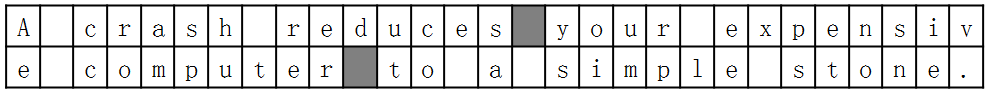
\includegraphics{images/regex-encoding-variable-width.png}

}

\caption{변동길이 일본 전통 하이쿠 표현}

\end{figure}

회색칸이 ``행의 끝(end of line)''을 의미한다. 이런 표기법은 더 유연하고,
공간을 덜 낭비하지만, N번째 행 앞으로 뒤로 건너뛰는 것은 어렵게 되었다.
이유는 각각이 다른 길이를 갖기 때문이다. 물론 행 종료를 표시하는데
무엇을 사용할지 결정해야하는 문제가 남았다. 불행히도, 유닉스에서는 행의
끝으로 개행 문자(newline) 한개, \texttt{\textbackslash{}n}으로 정했지만,
윈도우에서는 행의 끝으로 복귀문자(carriage return) 다음에 개행문자,
\texttt{\textbackslash{}r\textbackslash{}n} 으로 정했다.

편집기 대부분에서 이런 차이를 탐지하고 처리할 수 있지만, 유닉스와
윈도우를 모두 다뤄야 되는 프로그래머에게는 여전히 성가신 일이다. 윈도우
운영체제 파일에서 데이터를 불러읽어올 경우, 파이썬에서
\texttt{\textbackslash{}r\textbackslash{}n} 을
\texttt{\textbackslash{}n} 으로 전환하고, 데이터를 써서 저장할 경우 반대
방식으로 전환한다. 그러나 이미지, 소리 또는 기타 이진 파일형식에서
\texttt{\textbackslash{}r} 또는 \texttt{\textbackslash{}n}에 해당하는
문자가 우연히 포함되어 있다면, 원치 않는 변환이 발생할 수 있다.

\hypertarget{localization}{%
\section{현지화/세계화}\label{localization}}

현지화(Localization)는 세계화(internationalization)의 동전의 양면과
같다. 세계화를 영어로 \texttt{internationalization}으로 길기 때문에
\texttt{i18n}으로 줄여서 현지화는 영어로 \texttt{Localization}으로 길기
때문에 동일한 로직으로 \texttt{L10N}으로 줄여 표현한다. 현지화에
해당되는 사항은 다음이 포함된다.
\autocite{oliver2023internationalization}

\begin{itemize}
\tightlist
\item
  문자 집합
\item
  통화
\item
  날씨 온도(\(^{\circ} C / ^{\circ} F\))
\item
  길이 (킬로미터, 마일)
\item
  날짜와 시간
\item
  키보드 배열
\item
  좌측에서 우축으로, 위에서 아래, 우측에서 좌측으로 텍스트 작성 방식과
  문서양식
\item
  \ldots{}
\end{itemize}

\hypertarget{uxacfc-pdf}{%
\chapter{\texorpdfstring{\LaTeX 과 PDF}{과 PDF}}\label{uxacfc-pdf}}

LaTeX(``라텍'' 혹은 ``레이텍''으로 읽음)을 간단히 정의하자면
\textbf{``논리적인 디자인''}이라고 할 수 있다. 작품이 생성되는
과정에서는 작가가 원고를 수기로 작성하거나 타자기로 입력한 뒤 이를
출판사에 제출한다. 그 후, 출판사의 편집 디자이너는 원고를 검토하여
세부적인 출력 형식을 결정하고 이를 인쇄소에 전달한다. 인쇄소에서는 이
정보를 바탕으로 과거에는 식자공이 식자판을 제작했으나, 현재는 컴퓨터가
파일을 생성한다. 그림~\ref{fig-latex-structure} 에 문서 디자인과 문서
논리 구조에 대해 이해를 위해 도식화했다.

미국 스탠포트 대학 크누스(Donald Knuth) 교수가 1978년에 만든 문서조판
프로그램을 TeX(``텍''으로 읽음)이라고 하고, 레슬리 램포트(Leslie
Lamport) 교수가 만든 TeX 매크로 팩키지를 라텍이라고 한다. 텍과 라텍의
탄생 역사를 살펴보면 문서 논리 구조와 디자인 분리가 갖는 문서 저작
장점을 잘 나타내고 있다. 저수준(low-level) 언어로, 사용자가 페이지
레이아웃이나 글꼴 설정 등을 직접 제어할 수 있지만, 복잡한 포맷을 만들기
위해 사용자가 직접 매크로를 작성해야 한다는 점에서 일반 저작자가
사용하기에는 한계도 분명히 존재했다.

라텍은 1980년대에 레슬리 램포트에 의해 개발되었고, 텍을 기반으로
개발된다. 텍 복잡성을 단순화하여 더 사용자 친화적인 인터페이스를
제공한다. 따라서, 문서 구조와 내용에 더 집중할 수 있도록
고수준(high-level) 언어를 제공하며, 다양한 템플릿과 패키지가 제공되어
사용자가 쉽게 복잡한 레이아웃과 기능을 구현할 수 있다. 라텍 문서는
내부적으로 텍 엔진을 사용하여 조판된다. \autocite{Kim2017}

\begin{itemize}
\tightlist
\item
  라텍: 편집 디자이너의 역할에 해당하는 작업을 수행
\item
  텍: 식자공의 역할에 해당하는 작업을 수행
\end{itemize}

\begin{figure}

{\centering 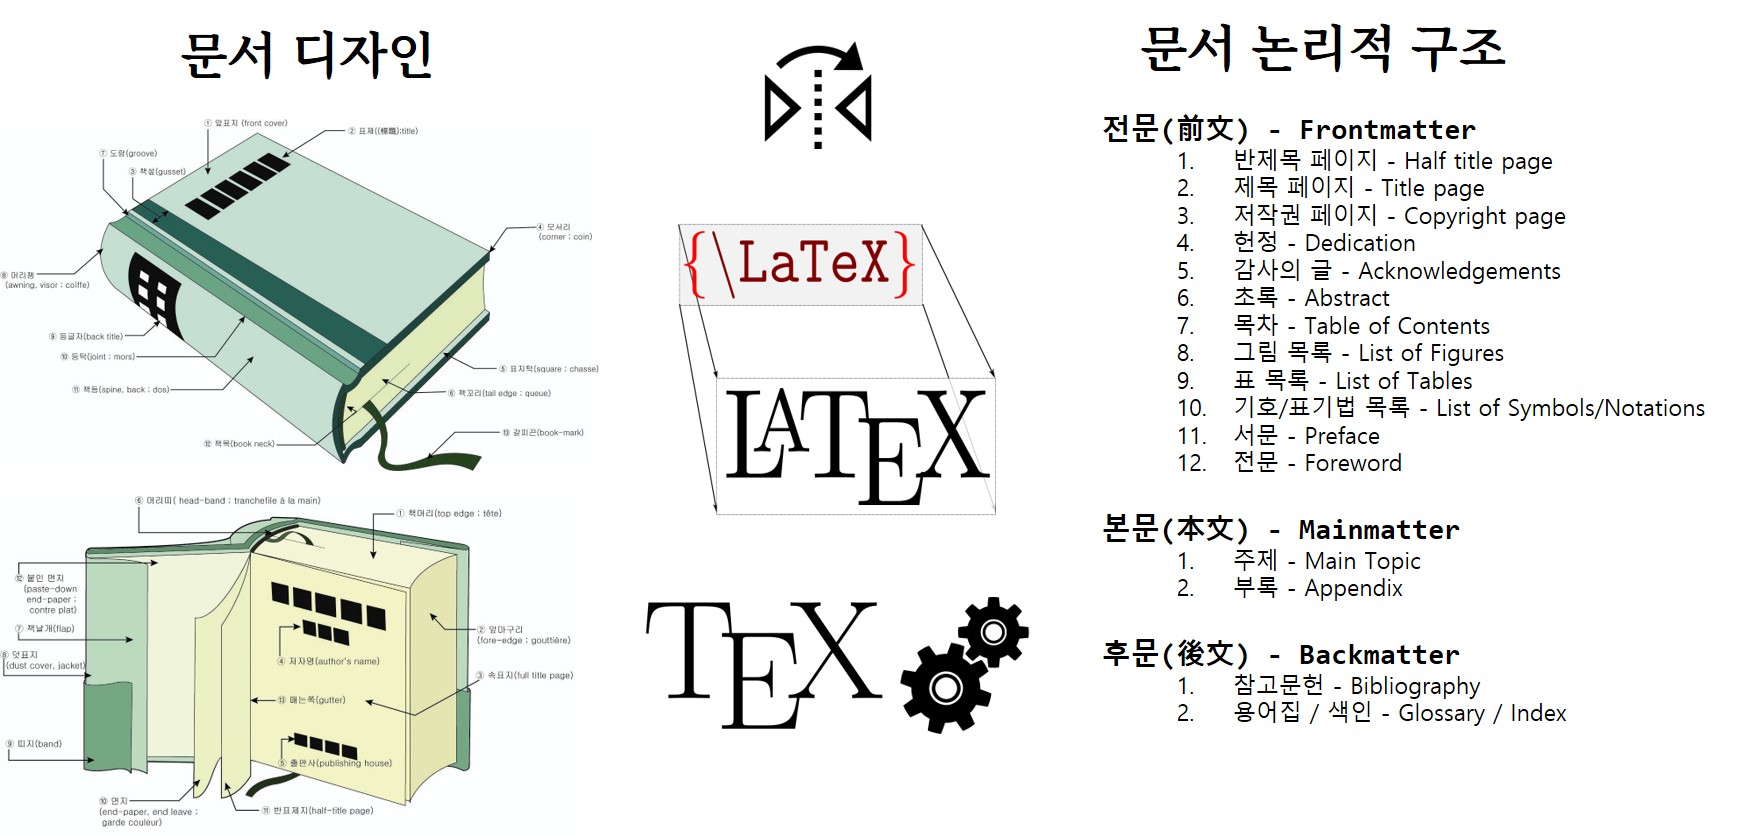
\includegraphics{images/document-logical-design.jpg}

}

\caption{\label{fig-latex-structure}문서 디자인과 문서 논리 구조}

\end{figure}

라텍에서 적용하는 논리적 디자인의 가장 큰 이점은 글쓰기 능력의 향상에
있다. 라텍으로 글을 작성하면서 점차 라텍의 논리적 디자인 철학에 맞춰가게
되며, 이를 통해 글쓰기 실력이 개선된다.

컴퓨터를 이용한 전자조판의 주된 목적은 문서를 읽기 쉽게 구성하여 저자의
의도를 독자에게 명확하게 전달하는 것이다. 이를 위해선 문서의 디자인이 그
내용의 논리적 구조를 잘 반영해야 하며, 이를 달성하기 위해서는 디자이너가
문서의 논리적 구조를 충분히 이해해야 한다. 라텍 명령어 체계는 기본적으로
이러한 \textbf{문서의 논리적 구조를 명시}하는 데 중점을 둔다. 이렇게
설정된 명령어는 텍 엔진을 통해 조판되어 최종적으로 원하는 결과물을
생성한다.

라텍의 가장 큰 장점 중 하나는 확실히 자동화 기능이다. 수식, 참고문헌,
표, 그래프의 번호를 자동으로 관리해주며, 복잡한 문서 구조도 쉽게 다룰 수
있다. 특히, 국내외 학술지에 논문을 제출할 때에는 템플릿만 변경하면
고품질의 논문을 쉽게 생성할 수 있다. 반면, 워드 프로세서를 사용할 경우
이러한 작업은 수동으로 해야 하며, 이로 인해 시간을 낭비하게 되고
결과물이 덜 정교하게 나올 수 있다. 결과적으로, 라텍을 사용하면 글쓰기
본질에 더 집중할 수 있으며, 이를 통해 저자의 생각과 의견을 더욱 솔직하고
명확하게 독자에게 전달할 수 있다.

\hypertarget{latex-engine}{%
\section{라텍 엔진}\label{latex-engine}}

라텍을 실제 문서 작성에 활용하기 위해서는 적절한 텍 배포판을 선택해야
한다. 이에 대해 \href{http://www.ktug.org/}{KTUG 한국 TeX 사용자 그룹}은
\(ko.TeX\) Live를 추천하고 있으며, 그 이유는 다음과 같다.
\autocite{Lee2017}

\begin{itemize}
\tightlist
\item
  라텍 엔진으로 \texttt{pdfLaTeX}, \texttt{XeLaTeX}, \texttt{LuaLaTeX}
  세 가지가 있으나, \texttt{XeLaTeX}은 유니코드 텍 엔진으로 동아시아
  언어(CJK)를 잘 지원하고, 트루타입 및 오픈타입 폰트를 자유롭게 선택할
  수 있어 인기가 높다.
\item
  운영체제에 따라 차이는 있지만, 실제 문서 작업에 라텍을 안정적으로
  설치하고 사용하기 위해서는 \texttt{TeX\ Live}가 \texttt{MikTeX}보다
  안정성과 사용자 지원 측면에서 우수하다.
\item
  텍 소스파일과 PDF 파일 간의 탐색 기능은 TexStudio IDE를 활용하여 쉽게
  이용할 수 있다.
\end{itemize}

과거에는 \texttt{latex+dvips+pspdf}를 사용한 전통적인 작업 흐름이
있었으며, 이 방식은 \texttt{pstricks}를 이용해 PDF 파일을 생성하는데
시간이 오래 걸리고, \texttt{eps} 파일만을 이미지로 사용할 수 있다는
한계가 있었다. 또 다른 방식인 \texttt{latex+dvipdfmx} 작업 흐름은 중간
단계로 \texttt{.dvi} 파일을 생성한 후 \texttt{dvipdfmx}를 이용해 PDF
파일을 만든다. 그러나 현재 가장 인기 있는 작업 흐름은 pdfLaTeX, XeLaTeX,
LuaLaTeX를 활용한 방식으로, 이는 \texttt{.tex} 소스파일에서 바로
\texttt{.pdf} 파일을 생성할 수 있다는 장점이 있다.

논문 외의 문서를 작성할 경우에는 한 단계 더 나아가 \texttt{memoir} 또는
\texttt{oblivoir} 클래스를 활용하는 것이 효율적이다. 이 방법은 이미
검증된 문서 템플릿을 기반으로 빠르게 PDF 문서를 생성할 수 있는 방법이다.

\begin{figure}

{\centering 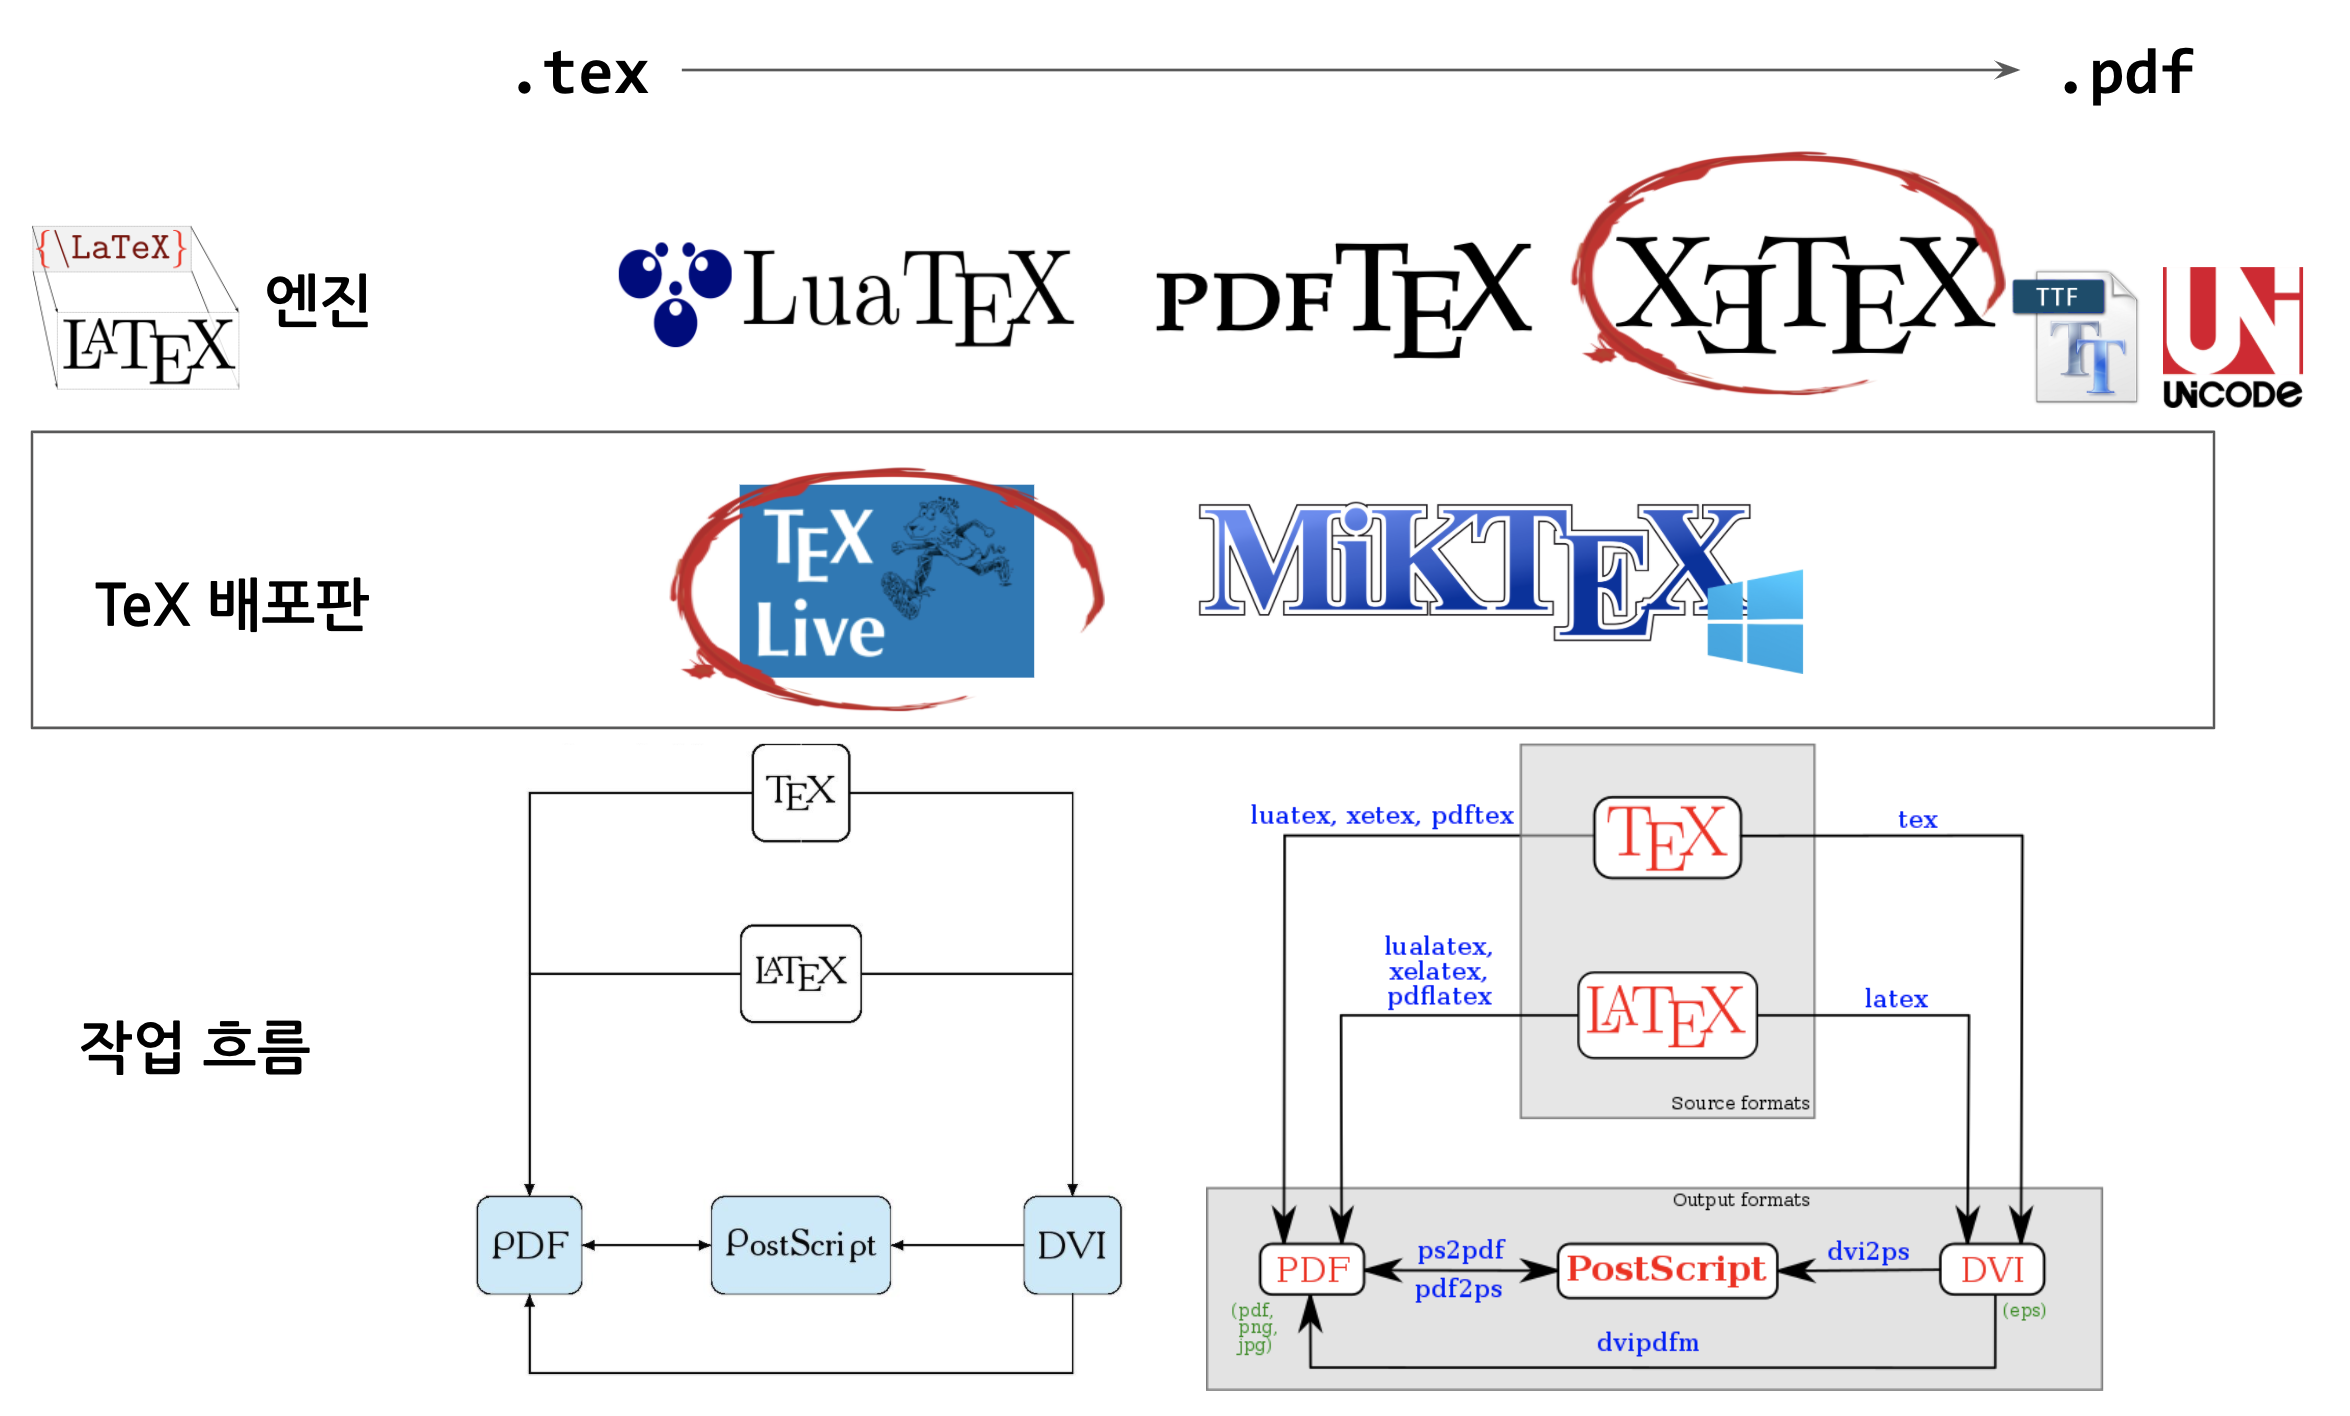
\includegraphics{images/tex-engines.png}

}

\caption{한글지원 라텍 엔진과 작업흐름}

\end{figure}

\hypertarget{latex-knuth}{%
\section{라텍 구성요소}\label{latex-knuth}}

수학과 교수였던 도널드 크누스는 문서 조판 시스템을 개발하면서 수식
처리를 간편하게 할 수 있도록 하면서, 메타폰트(METAFONT)라는 글꼴
시스템도 개발하여 고품질 글자체를 구현할 수 있도록 했다. 이러한 기초
위에 레슬리 램포트는 텍을 더욱 사용하기 쉽게 만들기 위해 다양한 매크로를
라텍으로 묶어 공개했다. 그 결과 일반인도 라텍을 이용해 고품질의 문서를
쉽게 작성할 수 있게 되었다. 버클리 대학 마이클 스피백 교수는 수식을
간편하게 문서에 적용할 수 있도록 AMS-TeX라는 매크로를 개발하고, 이에
대한 설명을 ``The Joy of TeX''이라는 책에서도 공개했다.
\autocite{spivak1990joy}

\texttt{pdftex}와 \texttt{e-TeX}이 결합하여 사실상
\href{http://wiki.ktug.org/wiki/wiki.php/TeX}{표준 TeX}이 되었고, 이를
기반으로 \href{http://wiki.ktug.org/wiki/wiki.php/XeTeX}{XeTeX}과
\texttt{LuaTeX}이 발전하고 있다. 특히, 한글 폰트 처리에 있어서
XeTeX(지텍으로 읽음)이 널리 사용되고 있다.

라텍 동작 원리는 Salomon의 도식화에 영감을 받아 Kees van der Laan이
1994년에 정리한 논문에서 상세하게 설명되어 있다. \autocite{van1994tex}
기본적으로 고품질의 전자 출판을 위해 글꼴과 텍이 필요하며, 이 두 요소가
결합하여 고품질의 출력물을 생성한다. 이러한 텍 엔진을 지원하는 다양한
패키지 중에서 \texttt{AMS-(La)TeX}, \texttt{LaTeX}, \texttt{manmac} 등이
주목을 받고 있다.

문서의 다양한 구성 요소, 예를 들어 \emph{목차}, \emph{색인},
\emph{참고문헌}, \emph{그림과 표} 등은 모듈화되어 관리되며, 글꼴 및
구조적인 스타일과 관련된 부분도 별도로 관리되고 있다.
\href{https://www.tug.org/texworks/}{TeXWorks}와 같은 위지윅(WYSIWYG)을
지원하는 편집기는 구문 강조, 맞춤법 검사 등을 통해 고품질의 라텍 문서
작성을 지원하고 있다.

\begin{figure}

{\centering 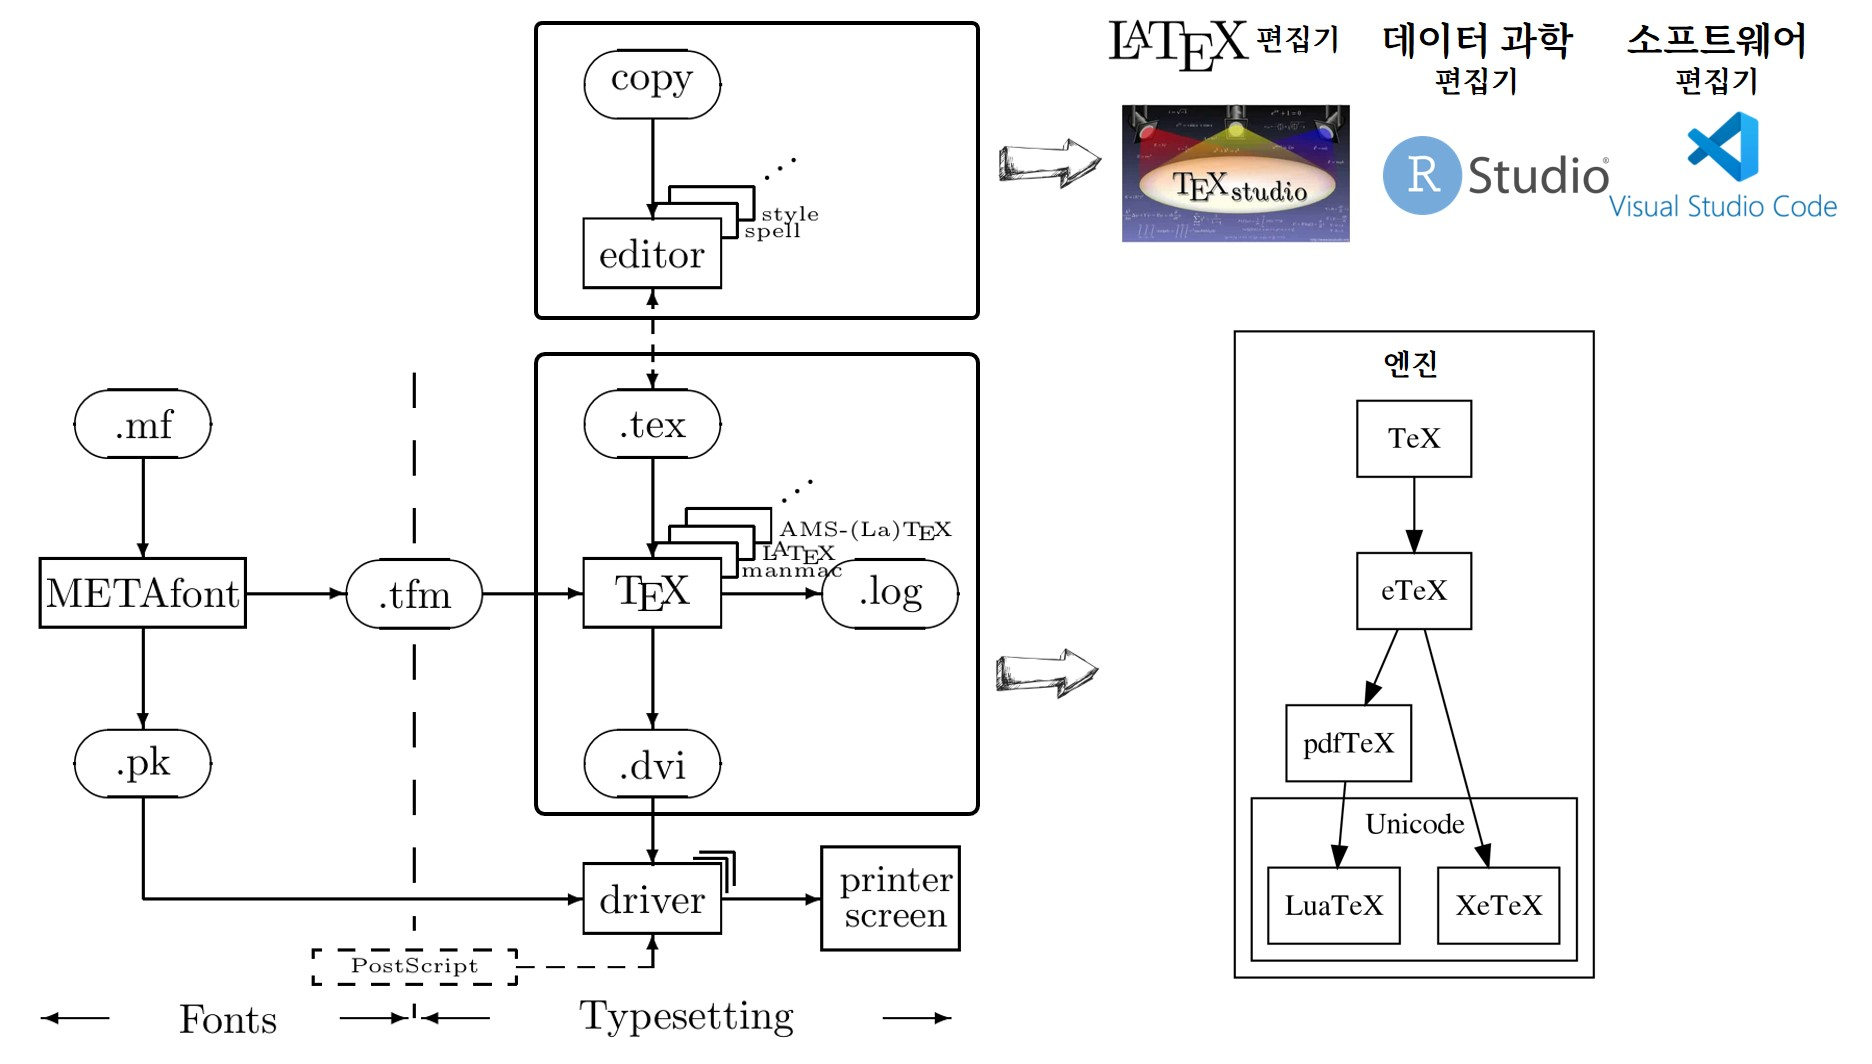
\includegraphics{images/latex_under_the_hood.jpg}

}

\caption{편집기, 엔진, 글꼴을 중심으로 본 \LaTeX 내부}

\end{figure}

라텍 문서 작성을 위해 기본적인 구성요소는 다음과 같다.

\begin{enumerate}
\def\labelenumi{\arabic{enumi}.}
\item
  \textbf{배포판:} 과거에는 다양한 배포판이 윈도우, 리눅스, 맥에서
  사용되었지만, 현재는 \href{https://www.tug.org/texlive/}{TeX Live}가
  대표적인 LaTeX 작업 환경이다. \href{http://miktex.org/}{MikTeX}도
  있지만, 큰 차이는 없다.
\item
  \textbf{글꼴:} 초기에는 글꼴로 폰트 메트릭(tfm)과 메타폰트(MetaFont)가
  주로 사용되었으나, 현재는 트루타입과 오픈타입이 널리 쓰인다.

  \begin{itemize}
  \tightlist
  \item
    폰트 선택은 밥처럼 기본적이면서도 안정적인 것이 좋다. 특별한
    상황에서는 그에 맞는 폰트를 선택하는 것이 중요하다.
  \item
    일반적으로 Serif와 San Serif 폰트를 한 쌍으로 사용하는 것이 균형감이
    있다. 예를 들어, 나눔고딕과 나눔명조, KoPub돋움과 KoPub바탕,
    함초롬도움과 함초롬바탕 등이 있다.
  \item
    글자 크기는 10\textasciitilde12 포인트가 적절하며, 이는 장시간
    동안의 읽기 피로를 줄이기 위함이다.
  \end{itemize}
\item
  \textbf{그래픽:} 텍/라텍 자체는 그래픽을 주요 영역으로 보지 않는다.
  과거에는 \texttt{dvips}와 EPS 형식을 주로 사용했으나, 현재는
  \texttt{.jpg}, \texttt{.png}, \texttt{.pdf} 등도 잘 처리한다.
\item
  \textbf{문자와 입력:} 초기에는 ASCII 코드가 주를 이루었으나, 현재는
  UTF-8을 권장하고 있다. 특히,
  \texttt{\textbackslash{}usepackage{[}utf8x{]}\{inputenc\}}가 필요한
  경우가 많다.
\item
  \textbf{색인과 참고문헌:} \texttt{makeindex}와 \texttt{bibtex}는
  색인과 참고문헌 처리의 표준이다. 그러나 유니코드 처리를 위해
  \texttt{texindy}와 \texttt{biber}도 주목을 받고 있다.
\item
  \textbf{수식:} 수학 표현과 관련해서는 미국 수학회가 발전시킨
  \textbf{amsmath}가 표준이다.
\item
  \textbf{출력:} 과거에는 \texttt{.dvi} 형식이 기본이었으나, 현재는
  \texttt{.pdf}가 기본이다. 또한, 웹을 위한 다양한 \texttt{.html} 출력도
  지원한다. 이에 따라, 웹이 책 형태의 문서보다 더 중요한 위치를 차지하게
  될 것으로 예상된다.
\end{enumerate}

\begin{Shaded}
\begin{Highlighting}[]
\CommentTok{\% A flowchart of a TeX workflow}
\CommentTok{\% Author: Stefan Kottwitz}
\CommentTok{\% https://www.packtpub.com/hardware{-}and{-}creative/latex{-}cookbook}
\BuiltInTok{\textbackslash{}documentclass}\NormalTok{[border=10pt]\{}\ExtensionTok{standalone}\NormalTok{\}}
\KeywordTok{\textbackslash{}begin}\NormalTok{\{}\ExtensionTok{document}\NormalTok{\}}
\FunctionTok{\textbackslash{}smartdiagram}\NormalTok{[flow diagram:horizontal]\{Edit,}
  \FunctionTok{\textbackslash{}LaTeX}\NormalTok{, Bib}\FunctionTok{\textbackslash{}TeX}\NormalTok{/ biber, make}\FunctionTok{\textbackslash{}{-}}\NormalTok{index, }\FunctionTok{\textbackslash{}LaTeX}\NormalTok{\}}
\KeywordTok{\textbackslash{}end}\NormalTok{\{}\ExtensionTok{document}\NormalTok{\}}
\end{Highlighting}
\end{Shaded}

라텍을 통한 PDF 파일 제작 과정은 몇 가지 주요 단계로 이루어진다. 라텍
전용 TexStudio 같은 통합개발환경(IDE), RStudio 같은 데이터 과학 IDE,
범용 소프트웨어 개발 VS코드 같은 IDE에서 텍스트 편집기를 열어 신규 라텍
파일을 생성하는데 파일 확장자는 \texttt{.tex}이다. 파일 시작 부분에
\texttt{\textbackslash{}documentclass} 명령어를 사용하여 문서의 종류와
옵션을 설정하는데, 학술 논문을 작성한다면 \texttt{article} 클래스를,
책을 작성한다면 \texttt{book} 클래스 등을 선택한다.

\texttt{\textbackslash{}usepackage} 명령어를 사용하여 필요한 패키지를
불러와서 특별한 기능이나 스타일을 추가한다. 예를 들어, 수식을 표현하기
위해 \texttt{amsmath} 패키지를, 그림을 삽입하기 위해 \texttt{graphicx}
패키지 등이 사용된다.

문서의 본문은 \texttt{\textbackslash{}begin\{document\}}와
\texttt{\textbackslash{}end\{document\}} 사이에 작성되고, 영역 안에서
텍스트, 표, 그림, 수식 등을 자유롭게 배치할 수 있다. 본문 작성 중에
참고문헌 서지관리를 위해 \texttt{BibTeX} \texttt{texindy},
\texttt{biber}를 사용하고, 색인 생성을 위해 \texttt{makeindex}를
사용한다.

본문 작성이 완료되면, 라텍 컴파일러를 실행하여 \texttt{.tex} 파일을
PDF로 변환한다. 영어는 \texttt{pdflatex}, 한글은 \texttt{xelatex} 을
라텍 엔진으로 사용하고, 참고문헌과 색인이 포함된 경우 컴파일 과정이
수차례 이어진다.

\begin{figure}

{\centering 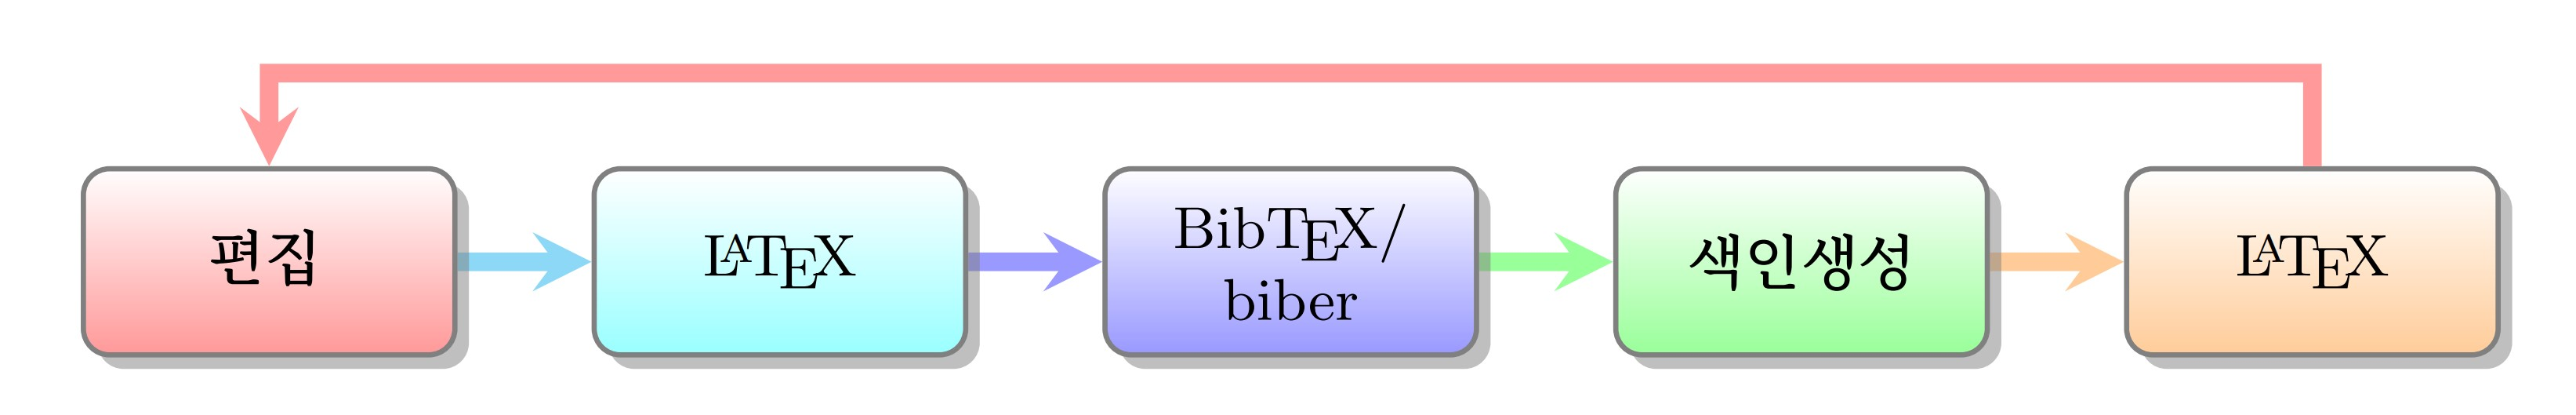
\includegraphics{images/latex_workflow.jpg}

}

\caption{라텍 작업흐름}

\end{figure}

\hypertarget{uxd658uxacbduxc124uxc815}{%
\section{환경설정}\label{uxd658uxacbduxc124uxc815}}

PDF는 기술적, 학술적, 사업적으로 혁신적인 문서 양식이다. PDF가 개발된
것은 오랜 역사를 자랑하지만 아래한글, 워드퍼펙트, MS 워드, 리브레 워드
등에 가려 그 진가를 발휘하지 못했다. 하지만 이제 PDF는 문서 출판의
최고봉이라는데 이의를 제기하는 사람은 없을 것이다. PDF 를 통해
아도비(Adobe) 회사는 엄청난 성공을 이어나가고 있고, 과학기술 저작에도
필수적인 파일 형태라 PDF에 대한 기본소양은 인공지능 시대를 살고 있는
시민으로 누구나 갖춰야하는 소양이다.

\hypertarget{uxb77cuxd14d-uxd658uxacbduxc124uxc815}{%
\section{라텍 환경설정}\label{uxb77cuxd14d-uxd658uxacbduxc124uxc815}}

라텍 설치와 사용은 처음에는 다소 복잡하게 느껴질 수 있다. 일반적으로
라텍 배포판(예: TeX Live, MiKTeX)을 설치한 뒤, 텍스트 에디터(예:
TeXShop, TeXworks)를 선택하여 작업환경을 구성한다. 설치가 완료되면,
\texttt{.tex} 파일을 생성하고 라텍 명령을 통해 PDF를 컴파일한다.

환경변수 설정, 패키지 관리, 글꼴 설정 등 세부적인 환경설정이 필요하다.
특히 한글 문서를 처리할 경우에는 \texttt{ko.TeX}나 \texttt{CTeX}와 같은
한글을 지원하는 패키지를 별도로 설치하고 한글 글꼴도 설정해야 한다.

\hypertarget{uxcffcuxd1a0-uxc124uxce58-2}{%
\subsection{쿼토 설치}\label{uxcffcuxd1a0-uxc124uxce58-2}}

\href{https://docs.posit.co/resources/install-quarto/}{Install Quarto}
웹사이트에 쿼토 설치 방법이 잘 설명되어 있다. 먼저 쉘에서
\texttt{curl}로 쿼토 설치파일을 다운로드 받는다. \texttt{gdebi-core}를
설치하고 다운로드 받은 쿼토 파일을 \texttt{gdebi} 명령어로 설치하고 나서
\texttt{quarto\ -\/-version} 명령어로 설치된 쿼토 버전을 확인한다.

\begin{Shaded}
\begin{Highlighting}[]
\ExtensionTok{$}\NormalTok{ sudo curl }\AttributeTok{{-}LO}\NormalTok{ https://quarto.org/download/latest/quarto{-}linux{-}amd64.deb}
\ExtensionTok{$}\NormalTok{ sudo apt{-}get install gdebi{-}core}
\ExtensionTok{$}\NormalTok{ sudo gdebi quarto{-}linux{-}amd64.deb}
\ExtensionTok{$}\NormalTok{ quarto }\AttributeTok{{-}{-}version}
\ExtensionTok{1.3.450}
\end{Highlighting}
\end{Shaded}

\hypertarget{uxb77cuxd14d-uxc124uxce58}{%
\subsection{라텍 설치}\label{uxb77cuxd14d-uxc124uxce58}}

\texttt{TinyTeX}은 \texttt{TeX\ Live}를 기반으로 한 경량, 이식성 좋고,
사용하기 쉬운 라텍 배포판으로 라텍 설치와 관련된 일반적인 불편함을
해결하기 위해 만들어졌고, 특히 ``이휘 쉬에(Yihui Xie)''가 개발하여 R과 R
마크다운 통합이 잘 되어 있다.

다른 라텍 배포판들이 수 기가바이트(GB)의 크기를 갖지만,
\texttt{TinyTeX}은 설치 크기가 작고 간단한 설치 과정을 제공으로 쉽지만
미려한 문서를 원하는 사용자들에게 인기가 많다. 특히, R과의 통합도 잘
이루어져 있어, 라텍 문서를 컴파일할 때 누락된 라텍 패키지도 자동으로
설치해주는 기능이 많은 사랑을 받고 있다.

보통 TexLive에 기반을 둔 \texttt{tinytex} 를 사용하는데 한글을 사용하는
입장에서는 \texttt{kotex}를 설치하는 방법도 모색이 필요하다. 유니코드
문자를 처리하기 위해서 \texttt{xelatex}을 쿼토 \(LaTeX\) 기본엔진으로
지정하면 \texttt{xelatex}을 통해 CJK 문자가 포함된 PDF 파일 제작이
가능하다.

쿼토를 설치하면 \texttt{quarto\ install\ tinytex} 명령어로
\texttt{TinyTeX}을 쉽게 설치할 수 있고, 설치 정보는
\texttt{quarto\ tools\ info\ tinytex}으로 파악이 가능하다.

\begin{Shaded}
\begin{Highlighting}[]
\ExtensionTok{$}\NormalTok{ quarto install tinytex}
\ExtensionTok{Installing}\NormalTok{ tinytex}
\ExtensionTok{[✓]}\NormalTok{ Downloading TinyTex v2023.09}
\ExtensionTok{[✓]}\NormalTok{ Unzipping TinyTeX{-}v2023.09.tar.gz}
\ExtensionTok{[✓]}\NormalTok{ Moving files}
\ExtensionTok{[✓]}\NormalTok{ Verifying tlgpg support}
\ExtensionTok{[✓]}\NormalTok{ Default Repository: https://mirrors.rit.edu/CTAN/systems/texlive/tlnet/}
\ExtensionTok{Installation}\NormalTok{ successful}

\ExtensionTok{$}\NormalTok{ quarto tools info tinytex}
\KeywordTok{\{}
  \StringTok{"name"}\ExtensionTok{:} \StringTok{"TinyTeX"}\NormalTok{,}
  \StringTok{"installed"}\ExtensionTok{:}\NormalTok{ true,}
  \StringTok{"version"}\ExtensionTok{:} \StringTok{"v2023.09"}\NormalTok{,}
  \StringTok{"directory"}\ExtensionTok{:} \StringTok{"/home/statkclee/.TinyTeX"}\NormalTok{,}
  \StringTok{"bin{-}directory"}\ExtensionTok{:} \StringTok{"/home/statkclee/.TinyTeX/bin/x86\_64{-}linux"}\NormalTok{,}
  \StringTok{"configuration"}\ExtensionTok{:}\NormalTok{ \{}
    \StringTok{"status"}\ExtensionTok{:} \StringTok{"ok"}
  \KeywordTok{\}}
\ErrorTok{\}}
\end{Highlighting}
\end{Shaded}

\texttt{kotex} 패키지 주요 장점 중 하나는 한글 관련 문제를 해결할 수
있는 다양한 라텍 패키지와 기본 한글 글꼴을 내장하고 있어 한글 문서
작성이 훨씬 편리하다. 하지만, \texttt{tinytex}를 기본 라텍 엔진으로
사용할 경우, 누락된 패키지로 인해 추가 작업이 어려울 수 있다. 이러한
문제를 해결하기 위해 \texttt{tinytex::parse\_install()} 함수를 사용하면,
오류가 발생한 텍스트를 붙여넣을 때 자동으로 필요한 패키지를 설치해 준다.
설치과정에서 오류 사항이 담긴 \texttt{.log} 파일을
\texttt{tinytex::parse\_install()} 함수에 인자로 넣어주면, 자동으로
필요한 패키지를 설치해 준다.

\begin{Shaded}
\begin{Highlighting}[]
\CommentTok{\# log 파일이 hello\_world.log}
\NormalTok{tinytex}\SpecialCharTok{::}\FunctionTok{parse\_install}\NormalTok{(}\StringTok{"hello\_world.log"}\NormalTok{)}

\NormalTok{tinytex}\SpecialCharTok{::}\FunctionTok{parse\_install}\NormalTok{(}
  \AttributeTok{text =} \StringTok{"! LaTeX Error: File \textasciigrave{}titlepic.sty\textquotesingle{} not found."}
\NormalTok{)}
\end{Highlighting}
\end{Shaded}

\begin{tcolorbox}[enhanced jigsaw, opacityback=0, opacitybacktitle=0.6, colback=white, rightrule=.15mm, coltitle=black, colframe=quarto-callout-note-color-frame, colbacktitle=quarto-callout-note-color!10!white, bottomrule=.15mm, bottomtitle=1mm, breakable, title=\textcolor{quarto-callout-note-color}{\faInfo}\hspace{0.5em}{\texttt{tinytex} 설치}, titlerule=0mm, leftrule=.75mm, toptitle=1mm, left=2mm, arc=.35mm, toprule=.15mm]

윈도우 환경에서 쿼토로 PDF 파일 생성할 때 다음과 같은 오류가 발생하여
로그에 기록될 경우 \texttt{tinytex} R 패키지를 설치하고
\texttt{tinytex::install\_tinytex()} 명령어로 \texttt{tinytex}를 다시
설치한다.

\begin{Shaded}
\begin{Highlighting}[]
\ExtensionTok{running}\NormalTok{ xelatex }\AttributeTok{{-}}\NormalTok{ 1}

\ExtensionTok{No}\NormalTok{ TeX installation was detected.}

\ExtensionTok{Please}\NormalTok{ run }\StringTok{\textquotesingle{}quarto install tinytex\textquotesingle{}}\NormalTok{ to install TinyTex.}
\ExtensionTok{If}\NormalTok{ you prefer, you may install TexLive or another TeX distribution.}
\end{Highlighting}
\end{Shaded}

\end{tcolorbox}

\hypertarget{uxd5ecuxb85cuxc6d4uxb4dc}{%
\section{헬로월드}\label{uxd5ecuxb85cuxc6d4uxb4dc}}

영문으로 작성된 PDF 파일은 텍스트, 이미지, 표, 그래프, 다이어그램과 같은
다양한 문서 기본구성요소가 포함된다. 다양한 문서요소로 구성된 PDF 문서는
출력을 했을 때 또렷하고 가독성이 좋다. 하지만, 한글이 추가될 때 언어
호환성 문제가 발생하여 한글 텍스트가 깨지는 문제가 종종 발생된다.
문제해결방법 중 하나가 한글 글꼴을 명시적으로 설정하는 것이다.

한글 글꼴 설정을 통해 문제를 해결한 후에는 쿼토 마크다운(QMD) 형식으로
PDF 파일을 변환한다. 쿼토 마크다운을 사용하는 이유는 라텍보다 마크다운
문서의 작성이 더 생산적이며, 웹 출판을 중점적으로 고려한 결과, 다양한
형태와 아름다운 웹 출판물을 쉽게 제작할 수 있기 때문이다. 쿼토
마크다운을 사용하면 웹 출판을 기본으로 하면서, PDF 출판도 함께 진행할 수
있어 일거양득의 효과를 볼 수 있다.

\hypertarget{uxc601uxbb38-pdf}{%
\subsection{영문 PDF}\label{uxc601uxbb38-pdf}}

기본적인 라텍 문서 구조에 표, 수식, 다이어그램, 주석을 추가한 라텍 기본
문서를 작성한다.

\begin{Shaded}
\begin{Highlighting}[]
\BuiltInTok{\textbackslash{}documentclass}\NormalTok{\{}\ExtensionTok{article}\NormalTok{\}  }\CommentTok{\% 문서 클래스 지정. article은 학술 논문, 보고서 등에 적합하다.}

\BuiltInTok{\textbackslash{}usepackage}\NormalTok{\{}\ExtensionTok{tikz}\NormalTok{\}  }\CommentTok{\% tikz 패키지 추가. 그래픽을 그리기 위해 필요하다.}

\FunctionTok{\textbackslash{}title}\NormalTok{\{fathers of the atomic bomb\}  }\CommentTok{\% 문서의 제목 설정}
\FunctionTok{\textbackslash{}author}\NormalTok{\{Oppenheimer\}  }\CommentTok{\% 문서의 저자 설정}
\FunctionTok{\textbackslash{}date}\NormalTok{\{}\FunctionTok{\textbackslash{}today}\NormalTok{\}  }\CommentTok{\% 문서의 날짜 설정. \textbackslash{}today를 사용하여 오늘 날짜를 자동 입력한다.}

\KeywordTok{\textbackslash{}begin}\NormalTok{\{}\ExtensionTok{document}\NormalTok{\}  }\CommentTok{\% 문서의 본문 시작}

\FunctionTok{\textbackslash{}maketitle}  \CommentTok{\% 제목, 저자, 날짜를 출력}

\KeywordTok{\textbackslash{}section}\NormalTok{\{Introduction\}  }\CommentTok{\% "Introduction"이라는 섹션 생성}

\NormalTok{The name "Oppenheimer"}\FunctionTok{\textbackslash{}footnote}\NormalTok{\{Oppenheimer is pronounced in English as /ˈɒpənˌhaɪmər\} is a German{-}origin surname that is most famously associated with J. Robert Oppenheimer, the American physicist known as one of the "fathers of the atomic bomb."  }\CommentTok{\% 본문과 각주}

\KeywordTok{\textbackslash{}section}\NormalTok{\{Table\}  }\CommentTok{\% "Table"이라는 섹션 생성}
\NormalTok{Below is a simple table.}
\KeywordTok{\textbackslash{}begin}\NormalTok{\{}\ExtensionTok{center}\NormalTok{\}}
\KeywordTok{\textbackslash{}begin}\NormalTok{\{}\ExtensionTok{tabular}\NormalTok{\}\{|c|c|\}}
\FunctionTok{\textbackslash{}hline}
\NormalTok{Header 1 }\OperatorTok{\&}\NormalTok{ Header 2 }\FunctionTok{\textbackslash{}\textbackslash{}}  \CommentTok{\% 테이블의 헤더}
\FunctionTok{\textbackslash{}hline}
\NormalTok{Row 1, Col 1 }\OperatorTok{\&}\NormalTok{ Row 1, Col 2 }\FunctionTok{\textbackslash{}\textbackslash{}}  \CommentTok{\% 첫 번째 행}
\NormalTok{Row 2, Col 1 }\OperatorTok{\&}\NormalTok{ Row 2, Col 2 }\FunctionTok{\textbackslash{}\textbackslash{}}  \CommentTok{\% 두 번째 행}
\FunctionTok{\textbackslash{}hline}
\KeywordTok{\textbackslash{}end}\NormalTok{\{}\ExtensionTok{tabular}\NormalTok{\}}
\KeywordTok{\textbackslash{}end}\NormalTok{\{}\ExtensionTok{center}\NormalTok{\}  }\CommentTok{\% 테이블 종료}

\KeywordTok{\textbackslash{}section}\NormalTok{\{Equation\}  }\CommentTok{\% "Equation"이라는 섹션 생성}
\NormalTok{Here is a simple equation:}
\KeywordTok{\textbackslash{}begin}\NormalTok{\{}\ExtensionTok{equation}\NormalTok{\}}\SpecialStringTok{  }\CommentTok{\% 수식 환경 시작}
\SpecialStringTok{  f(x) = x\^{}2  }\CommentTok{\% 수식}
\KeywordTok{\textbackslash{}end}\NormalTok{\{}\ExtensionTok{equation}\NormalTok{\}  }\CommentTok{\% 수식 환경 종료}

\KeywordTok{\textbackslash{}section}\NormalTok{\{Diagram\}  }\CommentTok{\% "Diagram"이라는 섹션 생성}
\NormalTok{Here is a simple diagram:}
\KeywordTok{\textbackslash{}begin}\NormalTok{\{}\ExtensionTok{center}\NormalTok{\}}
\KeywordTok{\textbackslash{}begin}\NormalTok{\{}\ExtensionTok{tikzpicture}\NormalTok{\}  }\CommentTok{\% tikz로 그림을 그리기 시작}
  \FunctionTok{\textbackslash{}draw}\NormalTok{[{-}\textgreater{}] (0,0) {-}{-} (4,0);  }\CommentTok{\% x축 그리기}
  \FunctionTok{\textbackslash{}draw}\NormalTok{[{-}\textgreater{}] (0,0) {-}{-} (0,4);  }\CommentTok{\% y축 그리기}
  \FunctionTok{\textbackslash{}draw}\NormalTok{ (0,0) {-}{-} (3,3);  }\CommentTok{\% 대각선 그리기}
\KeywordTok{\textbackslash{}end}\NormalTok{\{}\ExtensionTok{tikzpicture}\NormalTok{\}}
\KeywordTok{\textbackslash{}end}\NormalTok{\{}\ExtensionTok{center}\NormalTok{\}  }\CommentTok{\% 그림 환경 종료}

\KeywordTok{\textbackslash{}end}\NormalTok{\{}\ExtensionTok{document}\NormalTok{\}  }\CommentTok{\% 문서의 본문 종료}
\end{Highlighting}
\end{Shaded}

RStudio로 라텍을 이용해 PDF 문서를 생성할 때, 먼저 새로운 \texttt{.tex}
문서를 생성하고 표, 수식, 다이어그램, 주석이 포함된 라텍 코드를
복사-붙여넣는다. RStudio의 \texttt{Compile\ PDF} 버튼을 클릭하여
컴파하고, 완료되면 PDF 문서가 자동으로 열린다.

\begin{figure}

{\centering 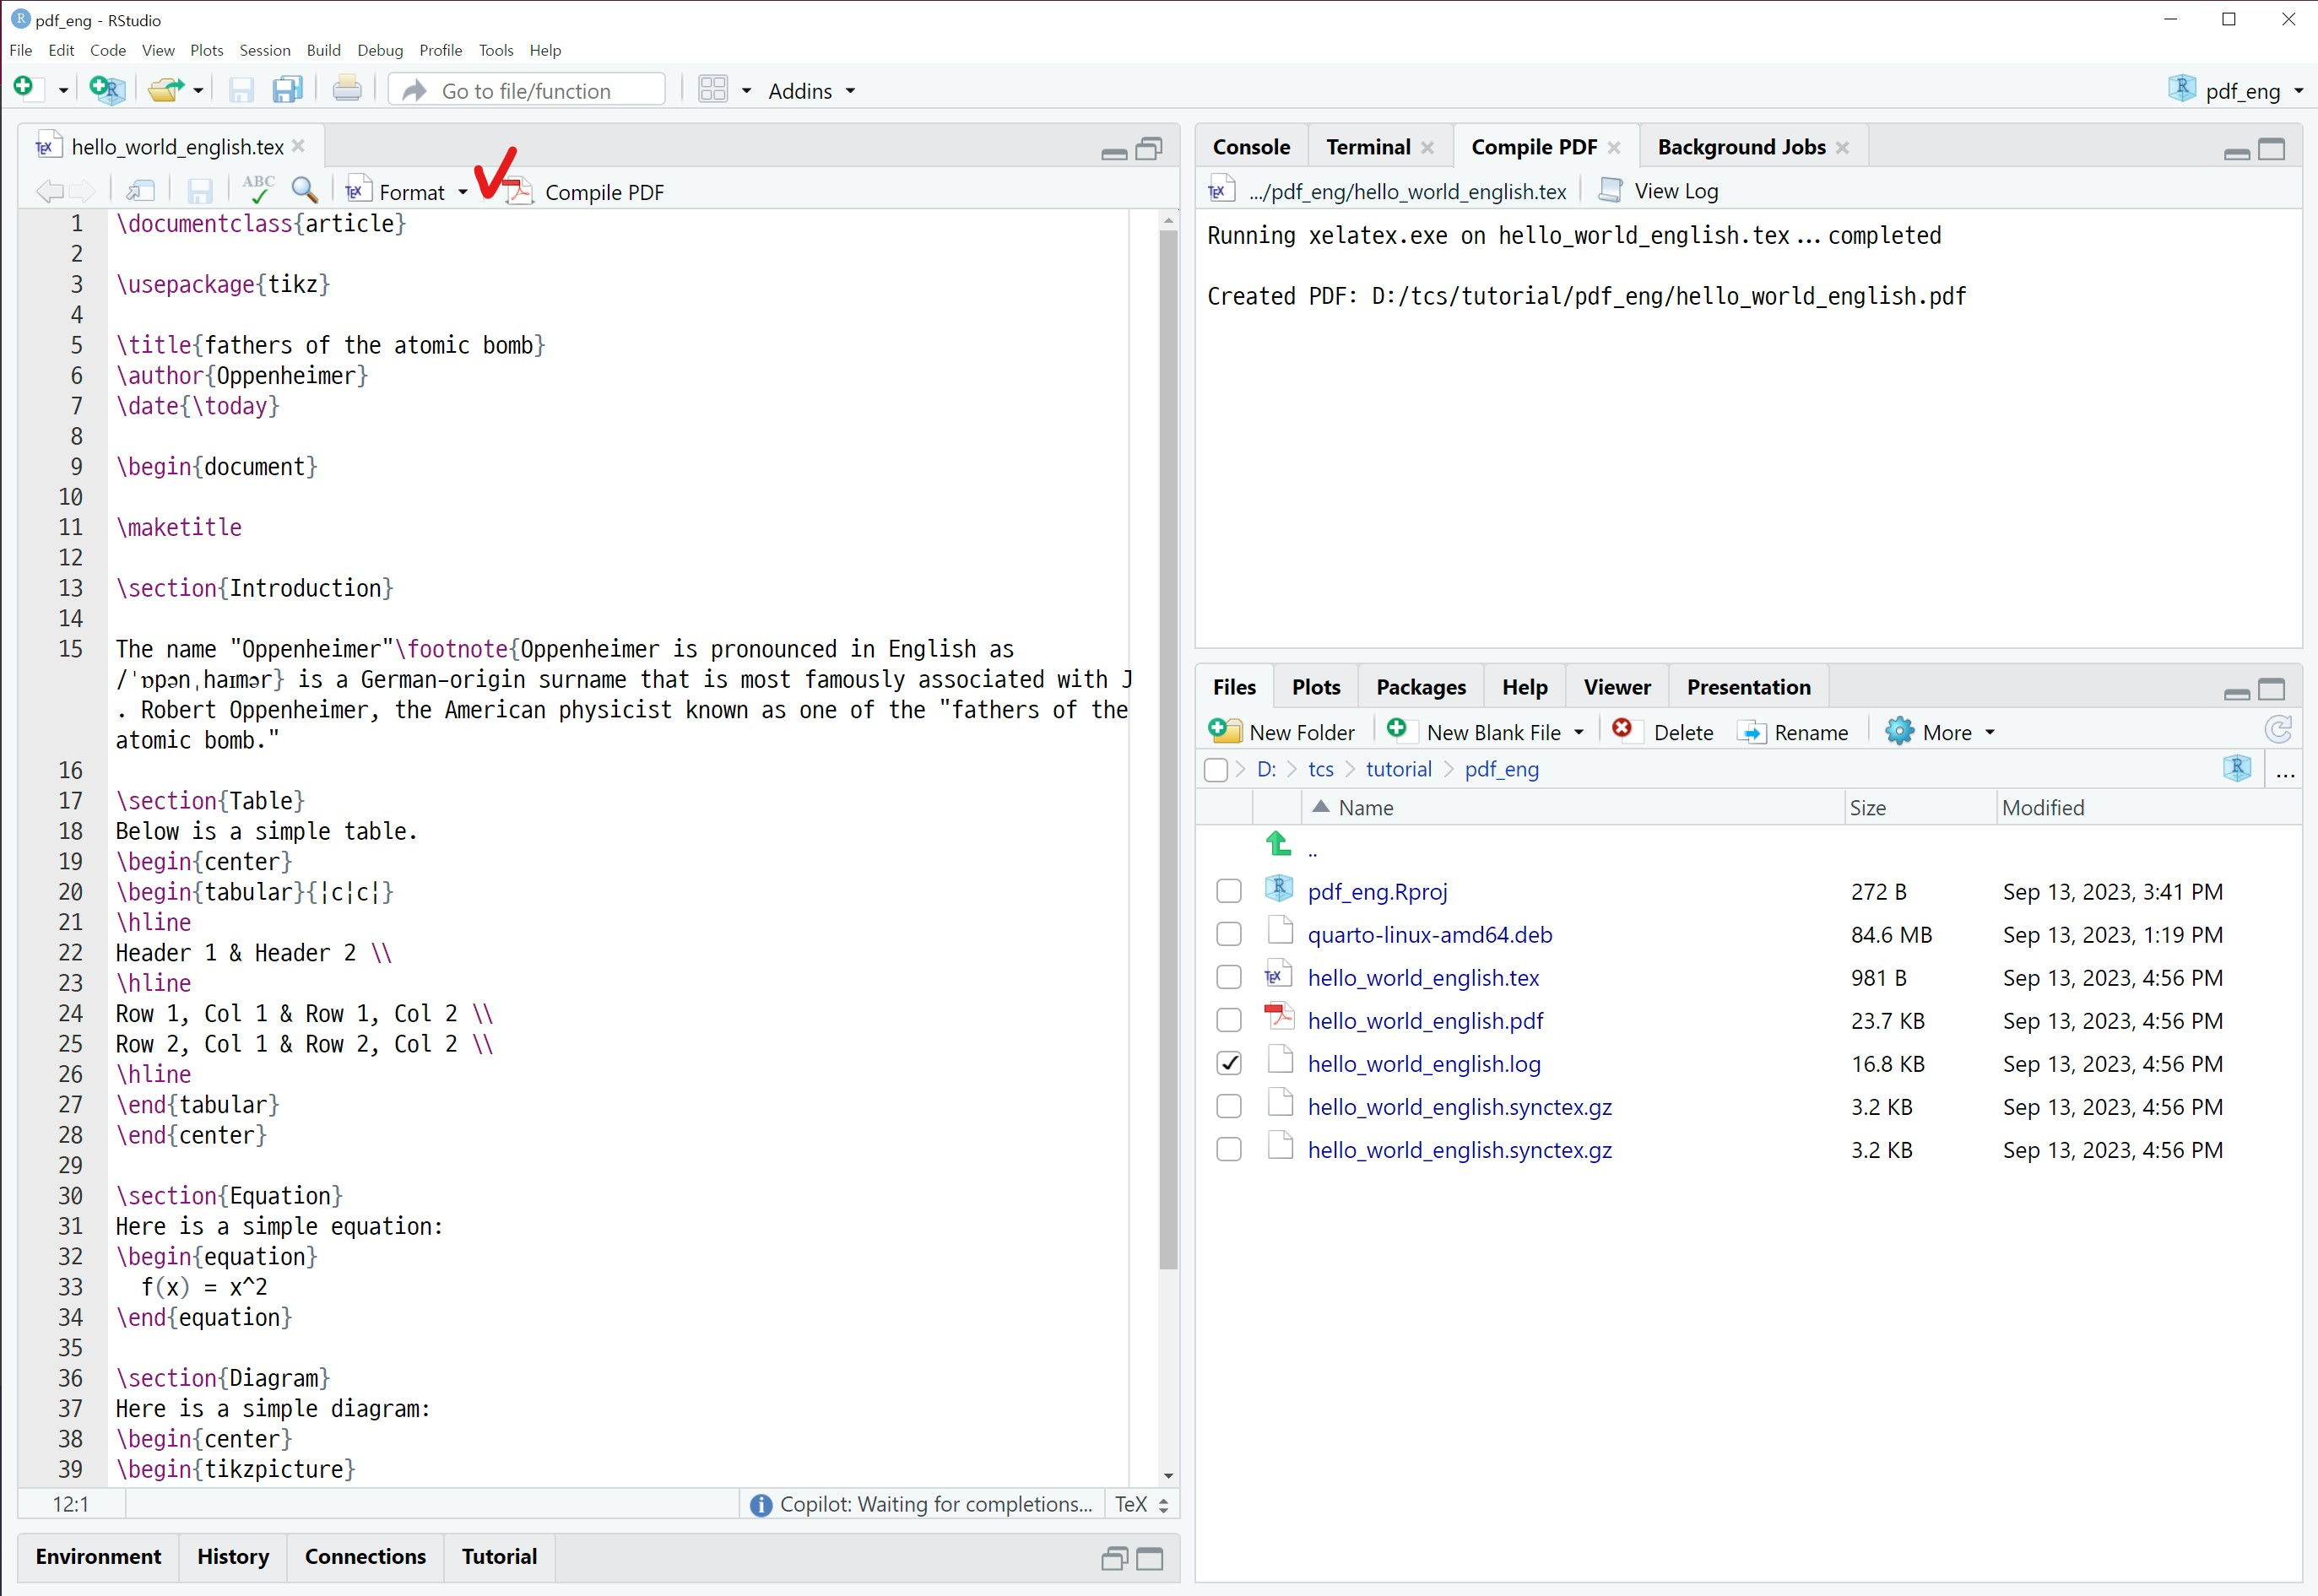
\includegraphics{images/pdf_english_rstudio.jpg}

}

\caption{라텍 문서 컴파일}

\end{figure}

\begin{figure}

{\centering 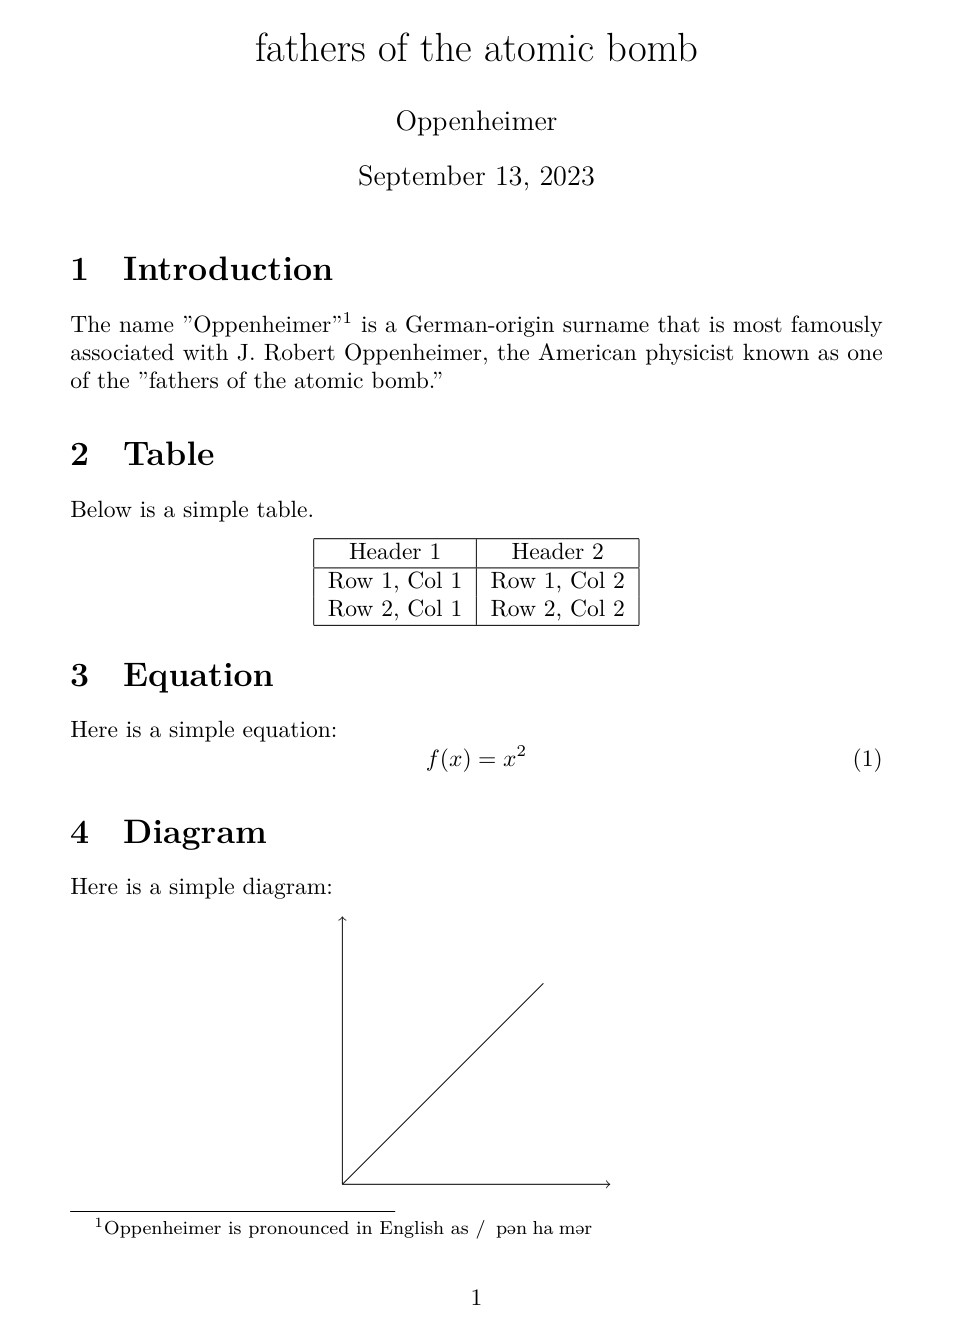
\includegraphics[width=2.66667in,height=\textheight]{images/pdf_english.jpg}

}

\caption{라텍 헬로월드 기본 문서}

\end{figure}

\hypertarget{uxd55cuxae00-pdf}{%
\subsection{한글 PDF}\label{uxd55cuxae00-pdf}}

영문 PDF를 한글로 번역하여 동일한 방식으로 PDF 파일을 만들기 위해
컴파일하게 되면 한글이 깨지거나 아무것도 없는 PDF 문서가 생성된다.

\begin{Shaded}
\begin{Highlighting}[]
\BuiltInTok{\textbackslash{}documentclass}\NormalTok{\{}\ExtensionTok{article}\NormalTok{\}}

\BuiltInTok{\textbackslash{}usepackage}\NormalTok{\{}\ExtensionTok{tikz}\NormalTok{\}}

\FunctionTok{\textbackslash{}title}\NormalTok{\{원자폭탄의 아버지들\}}
\FunctionTok{\textbackslash{}author}\NormalTok{\{오펜하이머\}}
\FunctionTok{\textbackslash{}date}\NormalTok{\{}\FunctionTok{\textbackslash{}today}\NormalTok{\}}

\KeywordTok{\textbackslash{}begin}\NormalTok{\{}\ExtensionTok{document}\NormalTok{\}}

\FunctionTok{\textbackslash{}maketitle}

\KeywordTok{\textbackslash{}section}\NormalTok{\{소개\}}

\NormalTok{"오펜하이머"라는 이름}\FunctionTok{\textbackslash{}footnote}\NormalTok{\{오펜하이머는 영어로 /ˈɒpənˌhaɪmər/ 로 발음된다\}은 독일 기원의 성씨로 가장 유명한 사람은 미국 물리학자 J. 로버트 오펜하이머이다. 그는 "원자폭탄의 아버지"로 알려져 있다.}

\KeywordTok{\textbackslash{}section}\NormalTok{\{표\}}
\NormalTok{아래는 간단한 표이다.}
\KeywordTok{\textbackslash{}begin}\NormalTok{\{}\ExtensionTok{center}\NormalTok{\}}
\KeywordTok{\textbackslash{}begin}\NormalTok{\{}\ExtensionTok{tabular}\NormalTok{\}\{|c|c|\}}
\FunctionTok{\textbackslash{}hline}
\NormalTok{헤더 1 }\OperatorTok{\&}\NormalTok{ 헤더 2 }\FunctionTok{\textbackslash{}\textbackslash{}}
\FunctionTok{\textbackslash{}hline}
\NormalTok{행 1, 열 1 }\OperatorTok{\&}\NormalTok{ 행 1, 열 2 }\FunctionTok{\textbackslash{}\textbackslash{}}
\NormalTok{행 2, 열 1 }\OperatorTok{\&}\NormalTok{ 행 2, 열 2 }\FunctionTok{\textbackslash{}\textbackslash{}}
\FunctionTok{\textbackslash{}hline}
\KeywordTok{\textbackslash{}end}\NormalTok{\{}\ExtensionTok{tabular}\NormalTok{\}}
\KeywordTok{\textbackslash{}end}\NormalTok{\{}\ExtensionTok{center}\NormalTok{\}}

\KeywordTok{\textbackslash{}section}\NormalTok{\{수식\}}
\NormalTok{다음은 간단한 수식이다:}
\KeywordTok{\textbackslash{}begin}\NormalTok{\{}\ExtensionTok{equation}\NormalTok{\}}
\SpecialStringTok{  f(x) = x\^{}2}
\KeywordTok{\textbackslash{}end}\NormalTok{\{}\ExtensionTok{equation}\NormalTok{\}}

\KeywordTok{\textbackslash{}section}\NormalTok{\{다이어그램\}}
\NormalTok{아래는 간단한 다이어그램이다:}
\KeywordTok{\textbackslash{}begin}\NormalTok{\{}\ExtensionTok{center}\NormalTok{\}}
\KeywordTok{\textbackslash{}begin}\NormalTok{\{}\ExtensionTok{tikzpicture}\NormalTok{\}}
  \FunctionTok{\textbackslash{}draw}\NormalTok{[{-}\textgreater{}] (0,0) {-}{-} (4,0);}
  \FunctionTok{\textbackslash{}draw}\NormalTok{[{-}\textgreater{}] (0,0) {-}{-} (0,4);}
  \FunctionTok{\textbackslash{}draw}\NormalTok{ (0,0) {-}{-} (3,3);}
\KeywordTok{\textbackslash{}end}\NormalTok{\{}\ExtensionTok{tikzpicture}\NormalTok{\}}
\KeywordTok{\textbackslash{}end}\NormalTok{\{}\ExtensionTok{center}\NormalTok{\}}

\KeywordTok{\textbackslash{}end}\NormalTok{\{}\ExtensionTok{document}\NormalTok{\}}
\end{Highlighting}
\end{Shaded}

\begin{figure}

{\centering 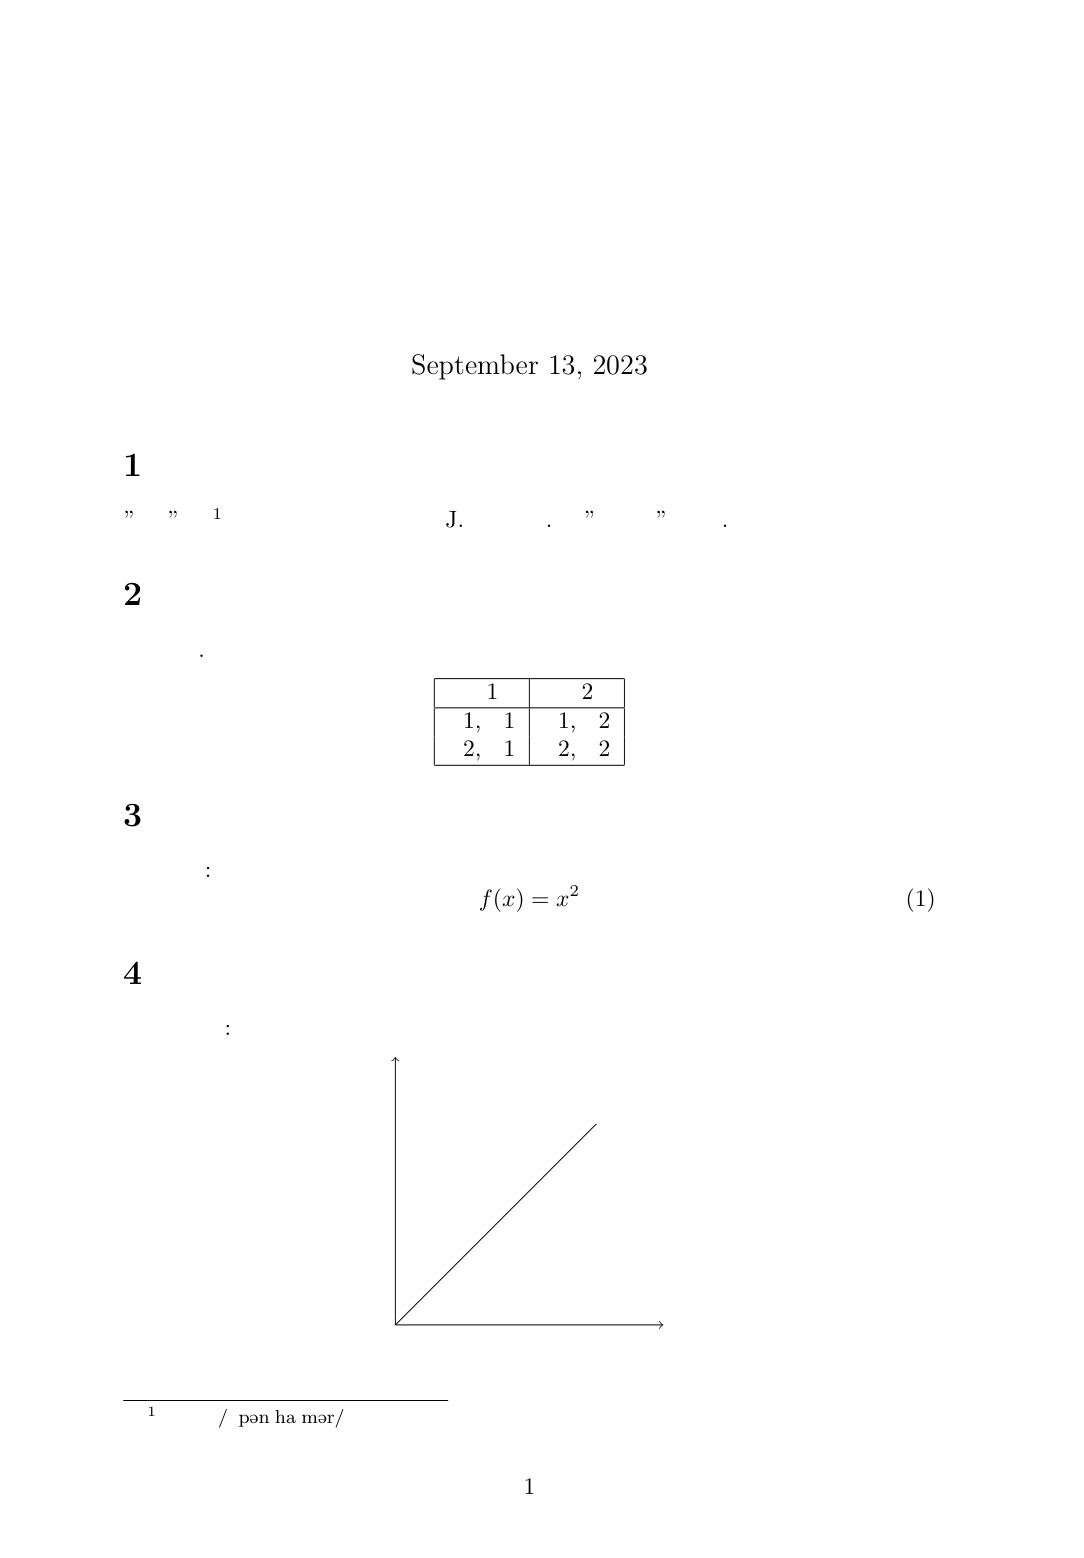
\includegraphics[width=2.54167in,height=\textheight]{images/pdf_korean.jpg}

}

\caption{LaTeX에서 한글이 깨진 PDF 문서}

\end{figure}

한글이 PDF 문서에 표현되지 않는 문제는 글꼴을 \texttt{.tex} 파일에
지정함으로써 해결된다. 먼저 전제조건으로 한글 글꼴(예를 들어, 나눔고딕
글꼴)이 설치되어 있고 이를 라텍 에서 컴파일하는 방식으로 작업한다.

\begin{Shaded}
\begin{Highlighting}[]
\BuiltInTok{\textbackslash{}documentclass}\NormalTok{\{}\ExtensionTok{article}\NormalTok{\}}

\BuiltInTok{\textbackslash{}usepackage}\NormalTok{\{}\ExtensionTok{tikz}\NormalTok{\}}
\BuiltInTok{\textbackslash{}usepackage}\NormalTok{\{}\ExtensionTok{fontspec}\NormalTok{\}}
\FunctionTok{\textbackslash{}setmainfont}\NormalTok{\{NanumGothic\} }\CommentTok{\% NanumGothic 글꼴이 설치되어야 함}
\BuiltInTok{\textbackslash{}usepackage}\NormalTok{\{}\ExtensionTok{tipa}\NormalTok{\} }\CommentTok{\% 발음기호(IPA symbols)}

\FunctionTok{\textbackslash{}title}\NormalTok{\{원자폭탄의 아버지들\}}
\FunctionTok{\textbackslash{}author}\NormalTok{\{오펜하이머\}}
\FunctionTok{\textbackslash{}date}\NormalTok{\{}\FunctionTok{\textbackslash{}today}\NormalTok{\}}

\KeywordTok{\textbackslash{}begin}\NormalTok{\{}\ExtensionTok{document}\NormalTok{\}}

\FunctionTok{\textbackslash{}maketitle}

\KeywordTok{\textbackslash{}section}\NormalTok{\{소개\}}

\NormalTok{"오펜하이머"라는 이름}\FunctionTok{\textbackslash{}footnote}\NormalTok{\{오펜하이머는 영어로 }\FunctionTok{\textbackslash{}textipa}\NormalTok{\{/ˈɒpənˌhaɪmər/\} , }\FunctionTok{\textbackslash{}textipa}\NormalTok{\{/}\FunctionTok{\textbackslash{}\textquotesingle{}}\NormalTok{\{O\}p@n}\FunctionTok{\textbackslash{}"}\NormalTok{\{h\}aIm@r/\} 로 발음된다\}은 독일 기원의 성씨로 가장 유명한 사람은 미국 물리학자 J. 로버트 오펜하이머이다. 그는 "원자폭탄의 아버지"로 알려져 있다.}

\KeywordTok{\textbackslash{}section}\NormalTok{\{표\}}
\NormalTok{아래는 간단한 표이다.}
\KeywordTok{\textbackslash{}begin}\NormalTok{\{}\ExtensionTok{center}\NormalTok{\}}
\KeywordTok{\textbackslash{}begin}\NormalTok{\{}\ExtensionTok{tabular}\NormalTok{\}\{|c|c|\}}
\FunctionTok{\textbackslash{}hline}
\NormalTok{헤더 1 }\OperatorTok{\&}\NormalTok{ 헤더 2 }\FunctionTok{\textbackslash{}\textbackslash{}}
\FunctionTok{\textbackslash{}hline}
\NormalTok{행 1, 열 1 }\OperatorTok{\&}\NormalTok{ 행 1, 열 2 }\FunctionTok{\textbackslash{}\textbackslash{}}
\NormalTok{행 2, 열 1 }\OperatorTok{\&}\NormalTok{ 행 2, 열 2 }\FunctionTok{\textbackslash{}\textbackslash{}}
\FunctionTok{\textbackslash{}hline}
\KeywordTok{\textbackslash{}end}\NormalTok{\{}\ExtensionTok{tabular}\NormalTok{\}}
\KeywordTok{\textbackslash{}end}\NormalTok{\{}\ExtensionTok{center}\NormalTok{\}}

\KeywordTok{\textbackslash{}section}\NormalTok{\{수식\}}
\NormalTok{다음은 간단한 수식이다:}
\KeywordTok{\textbackslash{}begin}\NormalTok{\{}\ExtensionTok{equation}\NormalTok{\}}
\SpecialStringTok{  f(x) = x\^{}2}
\KeywordTok{\textbackslash{}end}\NormalTok{\{}\ExtensionTok{equation}\NormalTok{\}}

\KeywordTok{\textbackslash{}section}\NormalTok{\{다이어그램\}}
\NormalTok{아래는 간단한 다이어그램이다:}
\KeywordTok{\textbackslash{}begin}\NormalTok{\{}\ExtensionTok{center}\NormalTok{\}}
\KeywordTok{\textbackslash{}begin}\NormalTok{\{}\ExtensionTok{tikzpicture}\NormalTok{\}}
  \FunctionTok{\textbackslash{}draw}\NormalTok{[{-}\textgreater{}] (0,0) {-}{-} (4,0);}
  \FunctionTok{\textbackslash{}draw}\NormalTok{[{-}\textgreater{}] (0,0) {-}{-} (0,4);}
  \FunctionTok{\textbackslash{}draw}\NormalTok{ (0,0) {-}{-} (3,3);}
\KeywordTok{\textbackslash{}end}\NormalTok{\{}\ExtensionTok{tikzpicture}\NormalTok{\}}
\KeywordTok{\textbackslash{}end}\NormalTok{\{}\ExtensionTok{center}\NormalTok{\}}

\KeywordTok{\textbackslash{}end}\NormalTok{\{}\ExtensionTok{document}\NormalTok{\}}
\end{Highlighting}
\end{Shaded}

\begin{figure}

{\centering 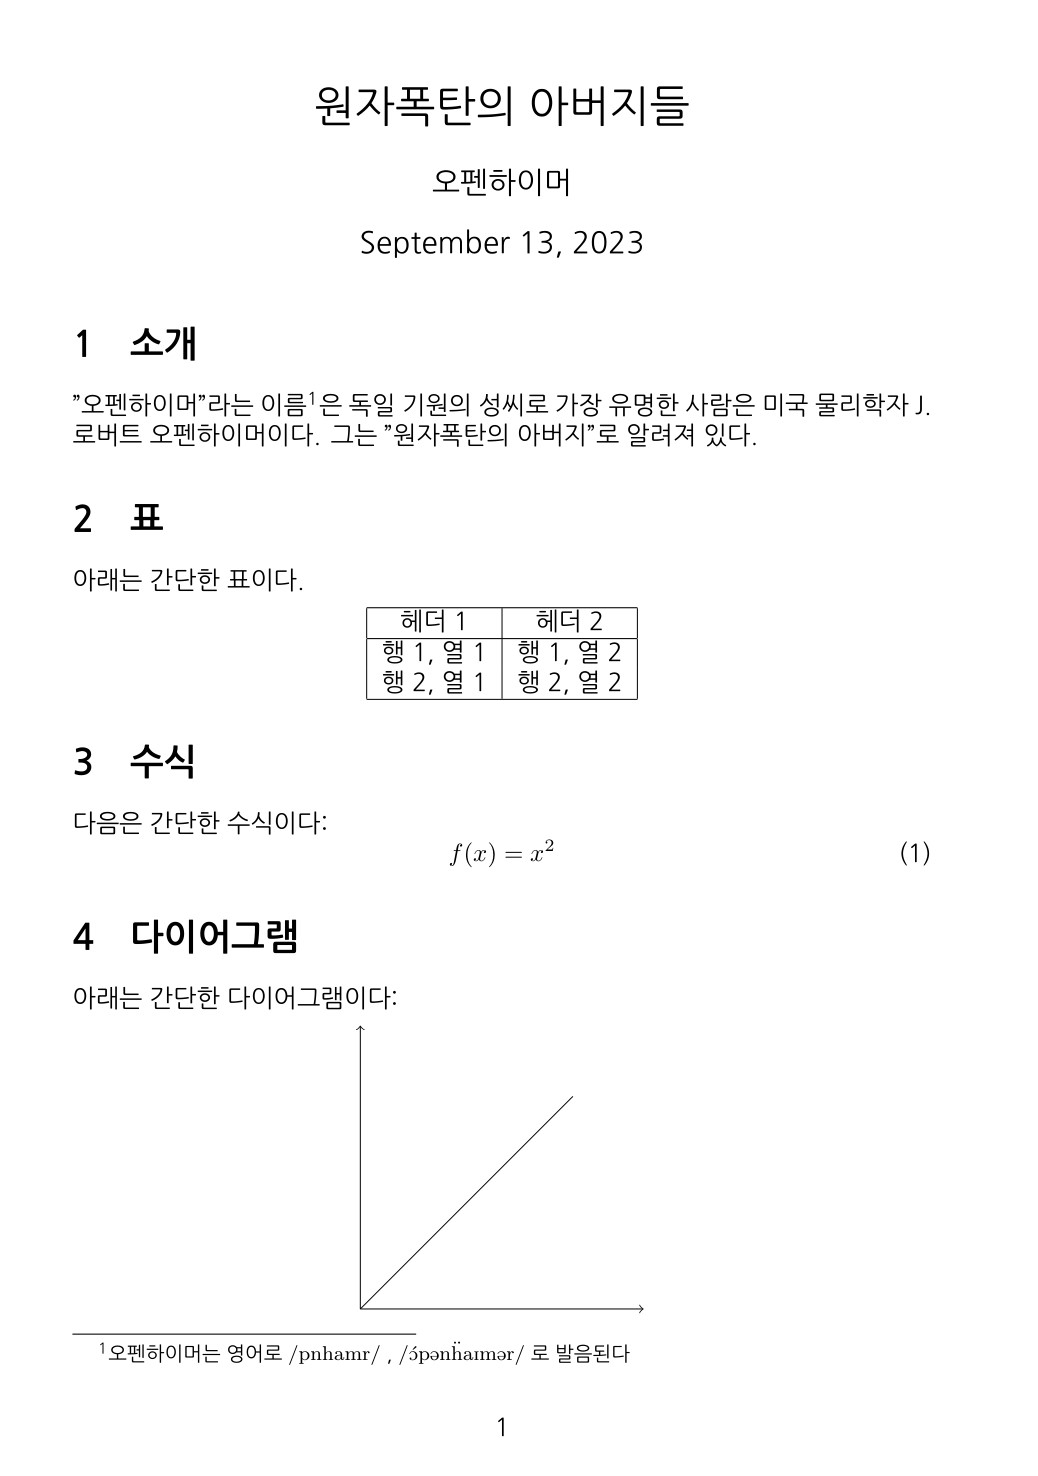
\includegraphics[width=2.5625in,height=\textheight]{images/pdf_korean_hangul.jpg}

}

\caption{\LaTeX 에서 한글문제를 해결한 PDF 문서}

\end{figure}

\hypertarget{uxcffcuxd1a0-pdf}{%
\subsection{쿼토 PDF}\label{uxcffcuxd1a0-pdf}}

PDF 문서 저작을 위해 쿼토 \texttt{.qmd} 파일에서 라텍 편집사항을
기술하려는 경우, 앞서 동일한 문서를 라텍 편집기가 아닌 쿼토 마크다운
파일로 작성한다.

\begin{Shaded}
\begin{Highlighting}[]
\ExtensionTok{{-}{-}{-}}
\ExtensionTok{title:} \StringTok{"원자폭탄의 아버지들"}
\ExtensionTok{author:} \StringTok{"오펜하이머"}
\ExtensionTok{date:} \StringTok{"2023{-}10{-}09"}
\ExtensionTok{format:} 
  \ExtensionTok{pdf:}
    \ExtensionTok{documentclass:}\NormalTok{ article}
    \ExtensionTok{geometry:}                                 
      \ExtensionTok{{-}}\NormalTok{ paperheight=257mm}
      \ExtensionTok{{-}}\NormalTok{ paperwidth=188mm}
      \ExtensionTok{{-}}\NormalTok{ top=25mm    }
      \ExtensionTok{{-}}\NormalTok{ headsep=10mm  }
      \ExtensionTok{{-}}\NormalTok{ bottom=30mm     }
      \ExtensionTok{{-}}\NormalTok{ footskip=15mm           }
      \ExtensionTok{{-}}\NormalTok{ left=25mm}
      \ExtensionTok{{-}}\NormalTok{ right=25mm}
      \ExtensionTok{{-}}\NormalTok{ centering       }
    \ExtensionTok{latex\_engine:}\NormalTok{ xelatex}
    \ExtensionTok{keep\_tex:}\NormalTok{ false}
    \ExtensionTok{include{-}in{-}header:}
      \ExtensionTok{text:} \KeywordTok{|}    
        \ExtensionTok{\textbackslash{}usepackage\{tikz\}}
        \ExtensionTok{\textbackslash{}usepackage\{fontspec\}}
        \ExtensionTok{\textbackslash{}usepackage\{tipa\}}
        \ExtensionTok{\textbackslash{}usepackage\{setspace\}}
        \ExtensionTok{\textbackslash{}onehalfspacing}

\ExtensionTok{mainfont:} \StringTok{"MaruBuri{-}Regular"}
\ExtensionTok{sansfont:} \StringTok{"NanumSquareR"}
\ExtensionTok{monofont:} \StringTok{"D2Codingligature"}
\ExtensionTok{editor\_options:} 
  \ExtensionTok{chunk\_output\_type:}\NormalTok{ console}
\ExtensionTok{{-}{-}{-}}

\CommentTok{\# 소개}

\StringTok{"오펜하이머"}\ExtensionTok{라는}\NormalTok{ 이름}\PreprocessorTok{[\^{}}\SpecialStringTok{1}\PreprocessorTok{]}\NormalTok{은 독일 기원의 성씨로 가장 유명한 사람은 미국 물리학자 J. 로버트 오펜하이머이다. 그는 }\StringTok{"원자폭탄의 아버지"}\NormalTok{로 알려져 있다.}

\ExtensionTok{[\^{}1]:}\NormalTok{ 오펜하이머는 영어로 }\DataTypeTok{\textbackslash{}t}\NormalTok{extipa\{/ˈɑpənˌhaɪmər\}\} 로 발음된다.}



\CommentTok{\# 표}

\ExtensionTok{아래는}\NormalTok{ 간단한 표이다.}

\ExtensionTok{:::}\NormalTok{ \{.cell\}}
\ExtensionTok{:::}\NormalTok{ \{.cell{-}output{-}display\}}


\KeywordTok{|}\ExtensionTok{헤더}\NormalTok{ 1     }\KeywordTok{|}\ExtensionTok{헤더}\NormalTok{ 2     }\KeywordTok{|}
\KeywordTok{|}\ExtensionTok{:{-}{-}{-}{-}{-}{-}{-}{-}{-}{-}}\KeywordTok{|}\ExtensionTok{:{-}{-}{-}{-}{-}{-}{-}{-}{-}{-}}\KeywordTok{|}
\KeywordTok{|}\ExtensionTok{행}\NormalTok{ 1, 열 1 }\KeywordTok{|}\ExtensionTok{행}\NormalTok{ 2, 열 1 }\KeywordTok{|}
\KeywordTok{|}\ExtensionTok{행}\NormalTok{ 1, 열 2 }\KeywordTok{|}\ExtensionTok{행}\NormalTok{ 2, 열 2 }\KeywordTok{|}


\ExtensionTok{:::}
\ExtensionTok{:::}


\CommentTok{\# 수식}

\ExtensionTok{다음은}\NormalTok{ 간단한 수식이다:}

\VariableTok{$$}
  \ExtensionTok{f}\ErrorTok{(}\ExtensionTok{x}\KeywordTok{)} \ExtensionTok{=}\NormalTok{ x\^{}2}
\VariableTok{$$}

\CommentTok{\# 다이어그램}

\ExtensionTok{아래는}\NormalTok{ 간단한 다이어그램이다:}

\ExtensionTok{:::}\NormalTok{ \{.cell layout{-}align=}\StringTok{"center"}\NormalTok{\}}
\ExtensionTok{:::}\NormalTok{ \{.cell{-}output{-}display\}}
\ExtensionTok{![]}\ErrorTok{(}\ExtensionTok{latex\_pdf\_files/figure{-}pdf/unnamed{-}chunk{-}4{-}1.pdf}\KeywordTok{)}\ExtensionTok{\{fig{-}align=}\StringTok{\textquotesingle{}center\textquotesingle{}}\ExtensionTok{\}}
\ExtensionTok{:::}
\ExtensionTok{:::}

\ExtensionTok{이} \KeywordTok{\textasciigrave{}}\ExtensionTok{.qmd}\KeywordTok{\textasciigrave{}}\NormalTok{ 파일은 Quarto를 사용하여 PDF로 렌더링할 수 있다. LaTeX 패키지와 명령어는 YAML 메타데이터의 }\KeywordTok{\textasciigrave{}}\ExtensionTok{header{-}includes}\KeywordTok{\textasciigrave{}}\NormalTok{ 섹션에 추가될 수 있다. 그러나 특별한 LaTeX 명령어나 환경이 필요한 경우, 이를 수동으로 }\KeywordTok{\textasciigrave{}}\ExtensionTok{.qmd}\KeywordTok{\textasciigrave{}}\NormalTok{ 파일에 적용해야 할 수도 있다.}
\end{Highlighting}
\end{Shaded}

\begin{figure}

{\centering 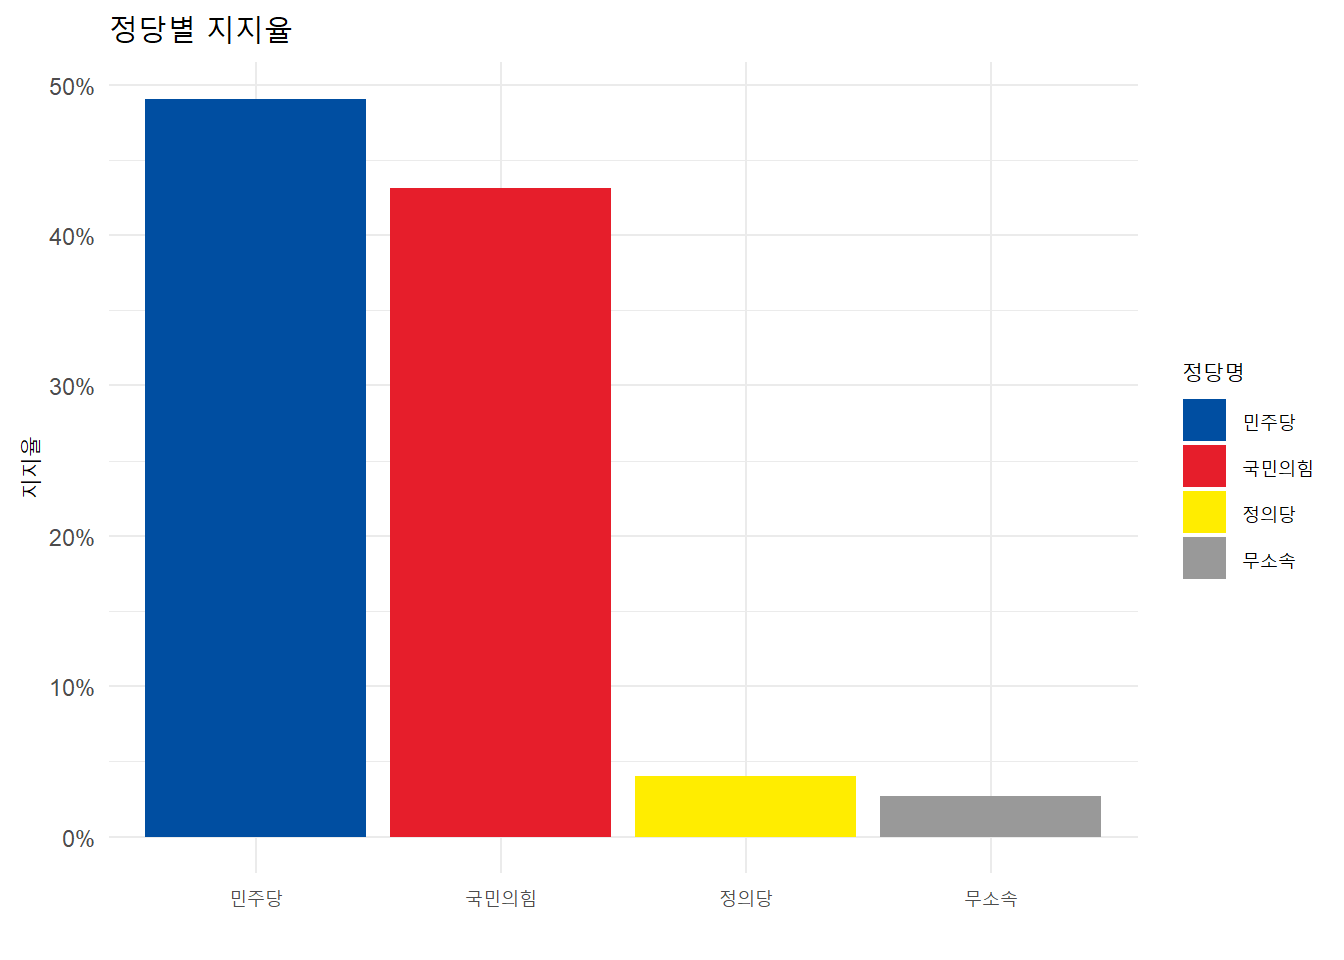
\includegraphics[width=3.35in,height=\textheight]{latex_pdf_files/figure-pdf/unnamed-chunk-5-1.png}

}

\caption{쿼토 마크다운으로 PDF 파일 생성}

\end{figure}

\hypertarget{uxcffcuxd1a0quarto}{%
\chapter{쿼토(Quarto)}\label{uxcffcuxd1a0quarto}}

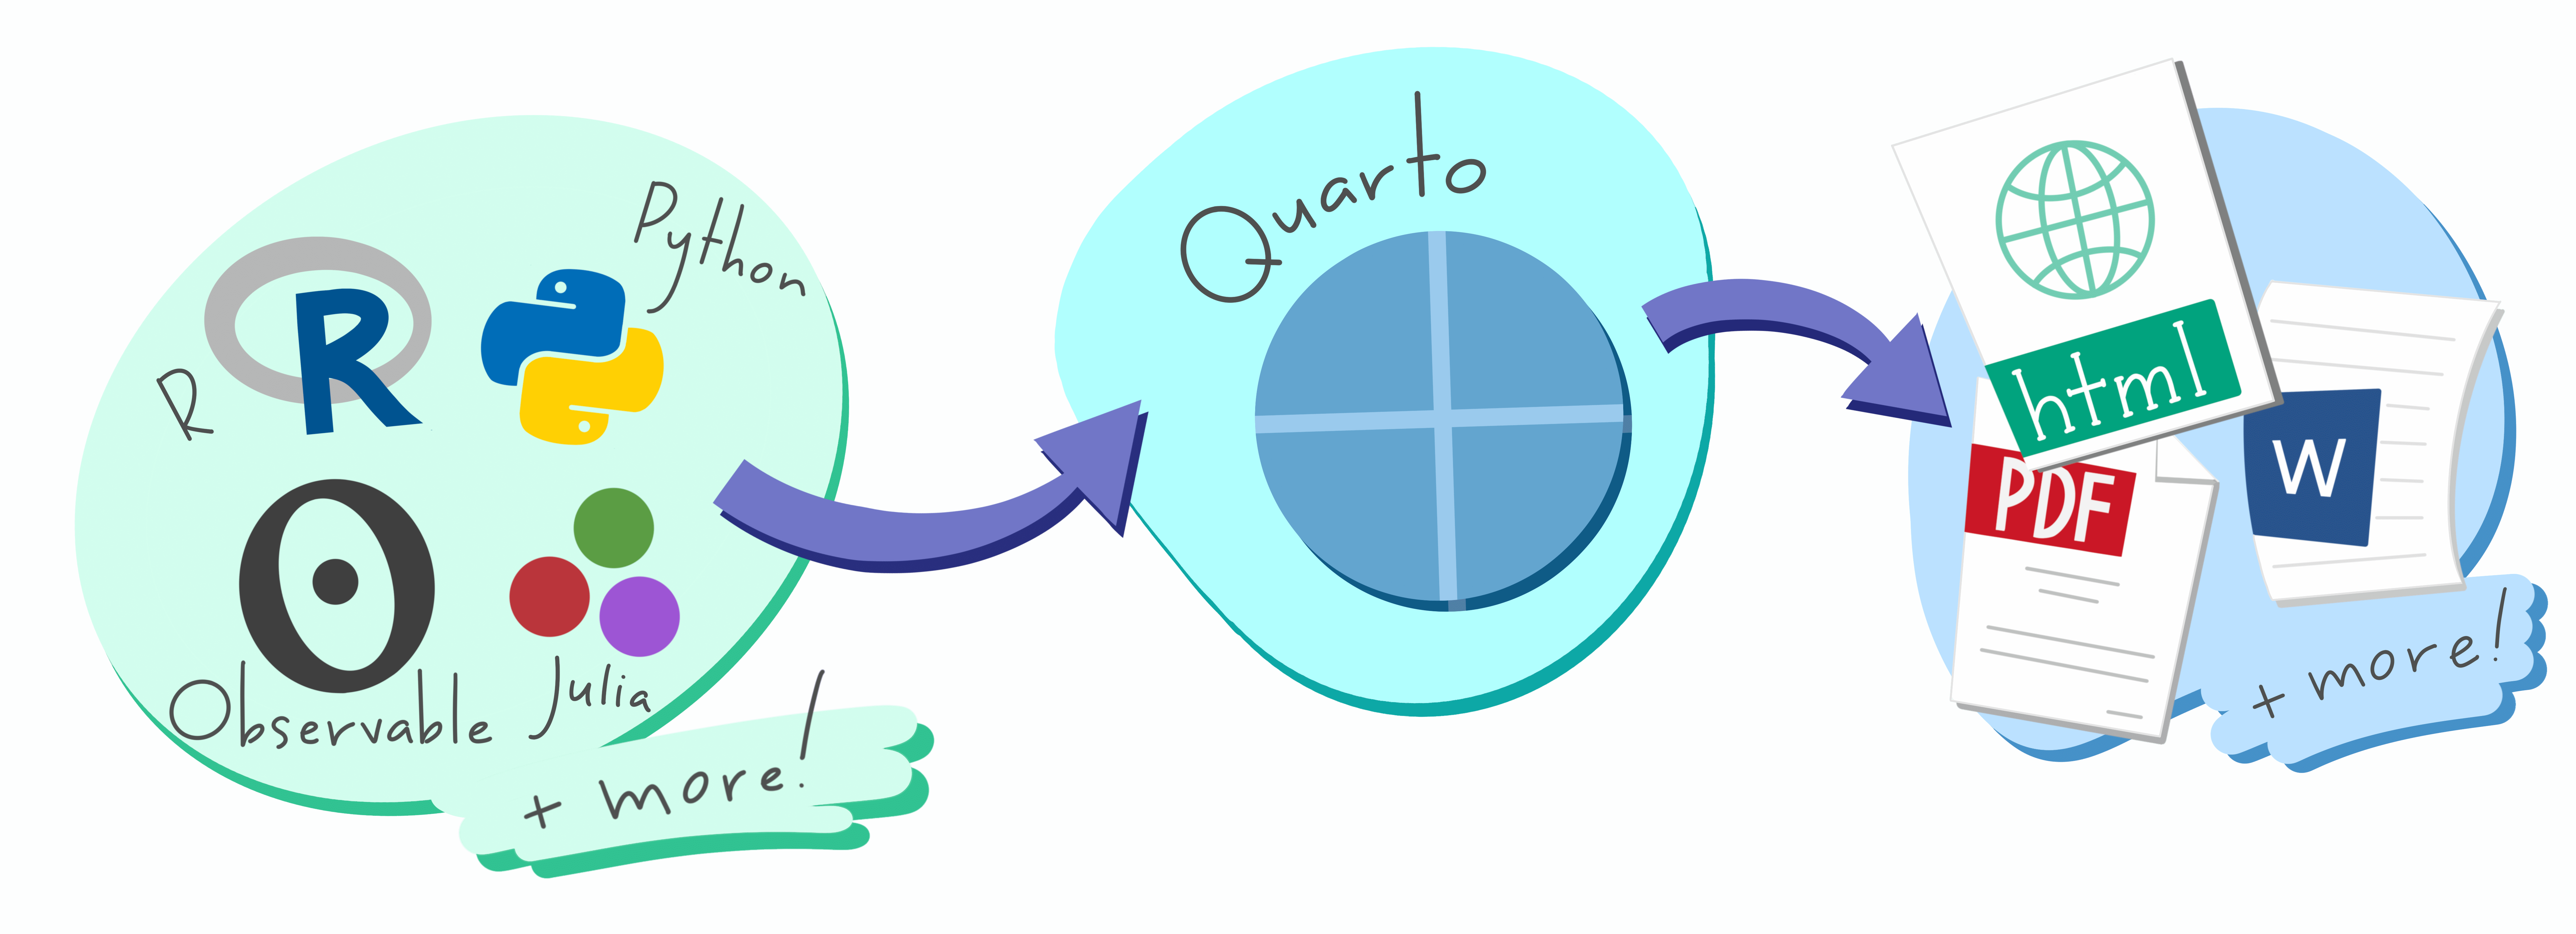
\includegraphics{images/horst_quarto_schematic.png}

쿼토(Quarto)는 다양한 프로그래밍 언어를 지원하는 오픈소스 출판
시스템으로, \href{https://pandoc.org/}{Pandoc}에 기반을 두고 있다.
쿼토는 R, 파이썬, 줄리아, 자바스크립트(Observable JS) 등의 프로그래밍
언어를 지원하며, 사용자는 싱글 소싱(Single Sourcing)을 통해 신속하게
다양한 출판 저작물을 생성할 수 있다. ``차세대 R마크다운(Next-Generation
R Markdown)''이라는 별명을 가진 쿼토는 약 10년 동안의 R 마크다운의
성공과 실패 경험을 바탕으로 새로운 아키텍처로 재탄생했다. 개발 및
유지보수 팀이 잘 구성되어 있어, 프로젝트의 지속 가능성과 신뢰성이 높고,
무료로 제공되므로 누구나 쉽게 접근할 수 있을 뿐만 아니라 누구나 오픈소스
프로젝트에 기여할 수 있다. \autocite{hyde2021single}

디지털 글쓰기와 출판에 대한 고민은 콘텐츠, 디자인, 형식의 세 가지로
나뉜다.

\begin{itemize}
\tightlist
\item
  \textbf{콘텐츠(Content)}: 저작물의 실질적인 내용으로 글쓰기 핵심이며,
  정보 정확성, 완전성, 통찰력을 제공해야 한다.
\item
  \textbf{디자인(Design)}: 저작물의 외양이나 'Look and Feel'을 의미하며
  사용자 경험에 큰 영향을 미치며, 정보를 효과적으로 전달하는 데 중요한
  역할을 한다.
\item
  \textbf{형식(Format)}: 저작물의 최종 형태나 산출물이 담기는
  매체(디지털, 인쇄 등)를 의미하며, 어떻게 배포되고 소비될 것인지
  결정한다.
\end{itemize}

쿼토는 세 가지 요소를 충족시키기 위한 다양한 기능을 제공한다.
팬독(Pandoc)과 마크다운을 활용해 수식, 인용, 서지 관리, 콜아웃, 고급
레이아웃 기능 등을 고품질 논문, 보고서, 발표 슬라이드(PPT), 웹사이트,
블로그, 전자책 등 다양한 형태 출판 산출물로 저작하여 인쇄매체 뿐만
아니라 HTML, PDF, MS 워드, ePub 등 다양한 디지털 매체를 통해 독자에게
전달할 수 있다. 특히, 쿼토는 프로그래밍 언어(R, 파이썬 등)와 문서 저작,
출판 산출물 사이 핵심 연결고리로 동작하여 버전 제어, 협업, 재현 가능한
과학기술 문서나 비즈니스에서 자동화된 생산성 높은 문서 저작에 큰 장점을
제공한다.

\begin{longtable}[]{@{}
  >{\centering\arraybackslash}p{(\columnwidth - 4\tabcolsep) * \real{0.2778}}
  >{\centering\arraybackslash}p{(\columnwidth - 4\tabcolsep) * \real{0.3889}}
  >{\centering\arraybackslash}p{(\columnwidth - 4\tabcolsep) * \real{0.3333}}@{}}
\toprule\noalign{}
\begin{minipage}[b]{\linewidth}\centering
프로그래밍(계산)
\end{minipage} & \begin{minipage}[b]{\linewidth}\centering
문서 저작
\end{minipage} & \begin{minipage}[b]{\linewidth}\centering
출력물
\end{minipage} \\
\midrule\noalign{}
\endhead
\bottomrule\noalign{}
\endlastfoot
Python, R, Julia, Observable JS & Pandoc, 마크다운,
\href{http://example.org}{\LaTeX} & 문서, 웹사이트, PPT, (전자)책,
블로그 등 \\
\end{longtable}

\hypertarget{uxc2f1uxae00-uxc18cuxc2f1-uxcd9cuxd310uxc800uxc791}{%
\section{싱글 소싱
출판저작}\label{uxc2f1uxae00-uxc18cuxc2f1-uxcd9cuxd310uxc800uxc791}}

데이터 과학을 비롯한 과학기술 분야 출판저작이 다른 분야와 약간 다를 수
있지만, 출판의 기본적인 접근 방식은 대체로 유사하다고 볼 수 있다. 특히,
싱글 소싱(Single Sourcing)\footnote{``싱글 소싱(Single Sourcing)''은
  하나의 원본 콘텐츠를 여러 형식이나 채널에 적용할 수 있도록 하는 문서
  작성 및 관리 방법이다. 콘텐츠를 한 번만 작성하고 다양한 출력 형식(예:
  PDF, 웹 페이지, PPT, 모바일 앱 등)으로 변환하게 되면, 콘텐츠 일관성
  유지 및 업데이트와 관리가 훨씬 효율적이다.} 방식을 통해 콘텐츠
저작부터 디자인, 협업, 검수, 최종 출판물 관리까지 일원화하고
자동화한다면, 중복작업과 낭비를 줄이는 동시에 재현 가능성을 높일 수 있어
과학기술 출판저작물에 있어 가장 이상적인 방법으로 평가받고 있다.

싱글 소싱 저작 방식은 데이터, 코드, 수식, 다이어그램, 텍스트 등 다양한
저작물 구성요소를 하나의 소스에서 관리함으로써, 수정이나 업데이트가
필요할 때 일관성을 유지하면서 효율적으로 저작작업을 수행할 수 있어 연구
결과의 정확성과 신뢰성을 높이기 위한 재현가능한 글쓰기를 중시하는
과학기술 분야에서 특히 강조되고 있으며, 싱글 소싱을 통한 자동화 생산성을
중시하는 비즈니스 글쓰기에서도 점차 글로벌 표준으로 자리를 잡아가고
있다.

\begin{figure}[H]

{\centering \includegraphics[width=7.13in,height=5.02in]{quarto_files/figure-latex/mermaid-figure-1.png}

}

\end{figure}

\hypertarget{uxc791uxc5c5uxd750uxb984}{%
\section{작업흐름}\label{uxc791uxc5c5uxd750uxb984}}

기존 R \texttt{.Rmd} 파일과 파이썬 \texttt{.ipynb} 파일을 \texttt{.qmd}
파일로 통일시킨 것은 쿼토의 주요 특징 중 하나이다. 이러한 통합은 다양한
프로그래밍 언어를 사용하는 복잡한 작업 흐름을 단순화시킬 수 있고 협업을
촉진한다. 저작자는 마크다운을 사용하여 콘텐츠를 작성하고, 프로그래밍
코드는 R, 파이썬, 자바스크립트, 줄리아 등 프로그래밍 언어로 작성한다.
텍스트와 프로그래밍 코드는 팬독(pandoc)을 통해 마크다운 변환이 자동으로
이루어지기 때문에 후속 작업에 대해 걱정할 필요가 없다. 싱글 소싱 개념이
팬독을 통해 자동화되어 원하는 저작 결과물을 효율적이고 빠르게 얻을 수
있어 저작작업 생산성을 크게 향상시키는 장점이 있다.

\begin{figure}

\begin{minipage}[t]{\linewidth}

{\centering 

\raisebox{-\height}{

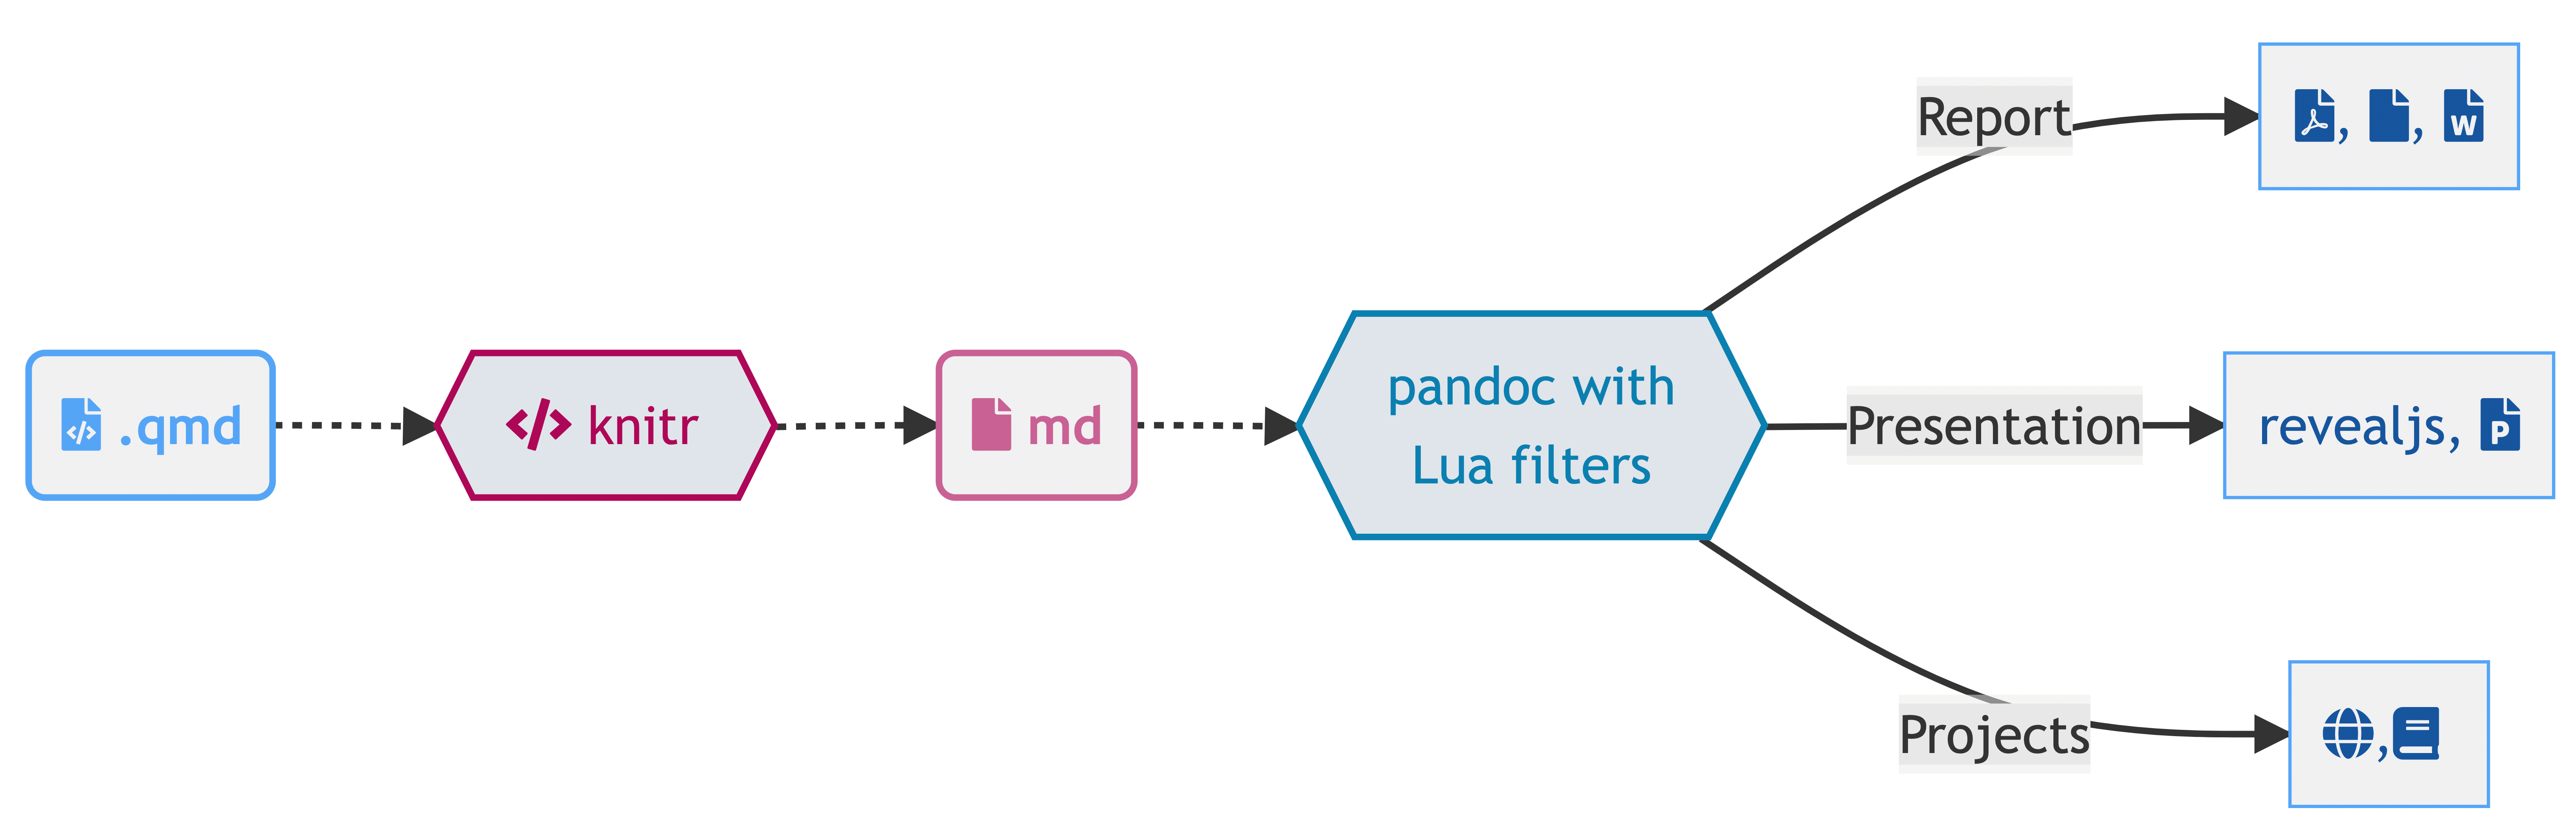
\includegraphics{images/qmd-knitr.png}

}

\caption{쿼토 - R}

}

\end{minipage}%
\newline
\begin{minipage}[t]{\linewidth}

{\centering 

\raisebox{-\height}{

\includegraphics{images/qmd-jupyter.png}

}

\caption{쿼토 - 파이썬}

}

\end{minipage}%

\caption{\label{fig-single-sourcing}쿼토 R, 파이썬 싱글소싱}

\end{figure}

\hypertarget{uxcffcuxd1a0-uxd574uxbd80}{%
\section{쿼토 해부}\label{uxcffcuxd1a0-uxd574uxbd80}}

쿼토는 데이터 과학 문서 작성의 새로운 패러다임을 제시하며, R마크다운의
후속임을 자처하고 있다. 10년 이상의 \texttt{knitr} 경험을 바탕으로
개발되었고, 최근에는 RStudio \textbf{Visual 편집} 기능을 통해
위지위그(What You See Is What You Get) 패러다임도 적극 수용함으로써
저작자는 복잡한 코드 작성 없이도 직관적으로 문서를 작성할 수 있게
되었다.

쿼토는 다양한 통합개발환경(IDE)과 호환성을 지원하고 있다. R 사용자는
RStudio IDE를, 파이썬 경험이 풍부한 사용자는 파이참, 범용 소프트웨어
개발 경험을 가지신 분은 VS코드, 이맥스/VIM 등과 통합하여 사용할 수 있고,
쿼토 CLI를 통해 IDE에서 쉽게 저작물을 다양한 형태로 출판할 수 있다.

쿼토는 다양한 프로그래밍 언어를 지원하여 문서 내에 계산(Computation)
기능을 쉽게 통합할 수 있는 현존하는 얼마 안되는 문학적 프로그래밍
저작도구다. R, 파이썬, SQL, 자바스크립트 등을 활용해 그래프, 표,
다이어그램, 인터랙티브 산출물을 문서에 반영하여 한층 진화된 디지털 문서
저작을 지원한다.

쿼토는 데이터 과학자, 개발자, 과학기술 연구원, 사무노동자 등 다양한
분야의 종사자분들로부터 챗GPT 인공지능 시대 자동화를 통한 사무업무
생산성 도구로 자리매김하고 있다.

\begin{figure}

{\centering \includegraphics{images/quarto-unification.png}

}

\caption{쿼토 작업흐름}

\end{figure}

쿼토 저작은 메타데이터(전문, front matter), 텍스트, 코드라는 세 가지
주요 구성요소로 이뤄진다. 쿼토는 문학적 프로그래밍과 자동화 패러다임을
적극 반영하여 데이터 과학 프로그래밍과 과학기술 문서 작성을 더
효율적이고 일관된 방식으로 저작하고 출판할 수 있도록 지원한다.

\begin{itemize}
\tightlist
\item
  \textbf{메타데이터 (YAML)}: YAML은 ``YAML Ain't Markup Language''의
  약자로, 데이터를 구조화하는 언어이다. 쿼토에서 이를 활용하여 문서
  전문(Front Matter)을 구성한다. 문서 상단에 위치하며 문서 제목, 작성자,
  날짜, 문서 형식 등을 포함하며 문서의 전반적인 설정과 구성을 담당한다.
\item
  \textbf{텍스트 (마크다운)}: 마크다운은 2004년에 아론 스워츠와 존
  그루버에 의해 개발된 언어로, HTML과 같은 복잡한 마크업 언어 대신
  사용되는 간단한 형식의 문서 작성 도구다. 복잡한 디자인보다 콘텐츠
  구조와 의미에 중점을 두기 때문에, 문서 저작자는 외양보다 내용에 더
  집중할 수 있다.
\item
  \textbf{코드 (\texttt{knitr}, \texttt{jupyter})}: \texttt{knitr}는 R
  코드를 문서에 통합할 수 있는 패키지, \texttt{jupyter}는 파이썬
  사용자에게 인기 있는 패키지이다. 쿼토에서는 이 두 패키지를 활용하여
  작성된 코드를 문서에 포함시킬 수 있다. 데이터 분석, 통계값, 그래프,
  다이어그램, 지도 등 다양한 코딩 결과물을 문서에 반영시킬 수 있다.
\end{itemize}

\begin{figure}

{\centering \includegraphics[width=4.6875in,height=\textheight]{images/quarto-anatomy.png}

}

\caption{쿼토 문서 구성요소}

\end{figure}

\hypertarget{yaml}{%
\subsection{YAML}\label{yaml}}

YAML(발음은 야믈)은 R 마크다운과 쿼토에서 주로 사용되는 경량언어다.
YAML은 문서 전문(front matter) 부분에 위치해 코드와 텍스트로 구성된 문서
본문보다 먼저 위치하며, 문서 메타데이터를 설정하는 역할을 수행한다.
쿼토에서 YAML을 이용해 문서 제목, 작성자, 날짜, 문서 형식, 레이아웃 등을
정의한다. YAML은 키와 값이 콜론(:)으로 구분되는 키값(key-value) 쌍을
사용해 각종 문서 설정정보를 표현하여 전반적인 문서 설정과 구성을 쉽게
관리한다.

\hypertarget{uxd0a4uxac12-uxc30d}{%
\subsection*{키값 쌍}\label{uxd0a4uxac12-uxc30d}}
\addcontentsline{toc}{subsection}{키값 쌍}

\begin{Shaded}
\begin{Highlighting}[]
\PreprocessorTok{{-}{-}{-}}
\FunctionTok{key}\KeywordTok{:}\AttributeTok{ value}
\PreprocessorTok{{-}{-}{-}}
\end{Highlighting}
\end{Shaded}

\hypertarget{uxbb38uxc11cuxcd9cuxb825uxd615uxc2dd-pdf-uxc9c0uxc815}{%
\subsection*{문서출력형식 PDF
지정}\label{uxbb38uxc11cuxcd9cuxb825uxd615uxc2dd-pdf-uxc9c0uxc815}}
\addcontentsline{toc}{subsection}{문서출력형식 PDF 지정}

\begin{Shaded}
\begin{Highlighting}[]
\PreprocessorTok{{-}{-}{-}}
\FunctionTok{format}\KeywordTok{:}\AttributeTok{ pdf}
\PreprocessorTok{{-}{-}{-}}
\end{Highlighting}
\end{Shaded}

YAML을 이용한 문서 전문 작성은 가독성이 뛰어나 읽고 이해하기 쉽다는
장점이 있다. 특히 복잡한 문서 구조나 설정을 지정할 때 유용하며, 중첩된
선택옵션 같은 복잡한 구조도 들여쓰기를 통해 명확하게 표현할 수 있다.
YAML은 재사용성이 뛰어나서 같은 설정 값을 여러 곳에서 사용해야 할 경우,
하나의 YAML 파일만 수정하면 모든 곳에 적용될 수 있어 시간과 노력을 크게
절약할 수 있다. 텍스트 기반인 만큼 Git과 같은 버전 제어 시스템과도 잘
통합되어, 여러 저자가 공동으로 작업할 때 진가를 발휘하지만, 들여쓰기에
민감하여 실수로 공백을 잘못 넣었을 경우 오류가 발생할 수 있어 주의가
필요하다.

YAML은 기본적으로 \texttt{KEY:\ Value} 형태로 구성되어 있지만, 이러한
단순한 구조 덕분에 매우 편리하고 유용하다. YAML을 통한 문서 저작을
경험하게 되면 YAML의 편리성과 유용함을 더 깊게 이해하게 된다.

\hypertarget{cli-pdf-uxc9c0uxc815}{%
\subsection*{CLI PDF 지정}\label{cli-pdf-uxc9c0uxc815}}
\addcontentsline{toc}{subsection}{CLI PDF 지정}

\begin{Shaded}
\begin{Highlighting}[]
\ExtensionTok{$}\NormalTok{ quarto render document.qmd }\AttributeTok{{-}{-}to}\NormalTok{ pdf}
\end{Highlighting}
\end{Shaded}

\hypertarget{yaml-uxbb38uxc11cuxd615uxc2dd-pdf}{%
\subsection*{YAML 문서형식
PDF}\label{yaml-uxbb38uxc11cuxd615uxc2dd-pdf}}
\addcontentsline{toc}{subsection}{YAML 문서형식 PDF}

\begin{Shaded}
\begin{Highlighting}[]
\PreprocessorTok{{-}{-}{-}}
\FunctionTok{format}\KeywordTok{:}\AttributeTok{ pdf}
\PreprocessorTok{{-}{-}{-}}
\end{Highlighting}
\end{Shaded}

\texttt{quarto\ render} 명령을 사용하여 \texttt{document.qmd} 파일을
\texttt{HTML} 형식으로 제작하는 예시에서 CLI 옵션
\texttt{-M\ code\ fold:true}을 사용하여 코드 섹션을 접을 수 있게
만들었다. 이러한 설정을 \texttt{YAML}로 바꾸면, 설정 파일 내에
\texttt{format} 섹션을 생성하고 그 안에 \texttt{html}을 정의한다. 그 후,
\texttt{html} 포맷 설정에 목차 생성(\texttt{toc:\ true})과 코드 접기
기능(\texttt{code-fold:\ true})을 추가한다.

CLI 옵션을 직접 입력하는 것과 비교하여 \texttt{YAML} 파일에 설정을 담는
것이 훨씬 깔끔하고 우아하다. CLI에서 많은 선택옵션을 직접 입력하면
명령어가 길어져 가독성이 떨어지고, 나중에 어떤 옵션을 사용했는지
확인하기 어렵다. 하지만 \texttt{YAML} 파일을 사용하면, 모든 설정을 한
곳에서 명확하게 관리할 수 있어 유지보수가 쉽고, 공동 저작자들과 공유와
협업에도 유리하다.

\hypertarget{cli-uxcf54uxb4dcuxc811uxae30}{%
\subsection*{CLI 코드접기}\label{cli-uxcf54uxb4dcuxc811uxae30}}
\addcontentsline{toc}{subsection}{CLI 코드접기}

\begin{Shaded}
\begin{Highlighting}[]
\ExtensionTok{$}\NormalTok{ quarto render document.qmd }\AttributeTok{{-}{-}to}\NormalTok{ html }\AttributeTok{{-}M}\NormalTok{ code fold:true}
\end{Highlighting}
\end{Shaded}

\hypertarget{yaml-uxcf54uxb4dcuxc811uxae30}{%
\subsection*{YAML 코드접기}\label{yaml-uxcf54uxb4dcuxc811uxae30}}
\addcontentsline{toc}{subsection}{YAML 코드접기}

\begin{Shaded}
\begin{Highlighting}[]
\PreprocessorTok{{-}{-}{-}}
\FunctionTok{format}\KeywordTok{:}\AttributeTok{ }
\AttributeTok{  }\FunctionTok{html}\KeywordTok{:}
\AttributeTok{    }\FunctionTok{toc}\KeywordTok{:}\AttributeTok{ }\CharTok{true}
\AttributeTok{    }\FunctionTok{code{-}fold}\KeywordTok{:}\AttributeTok{ }\CharTok{true}
\PreprocessorTok{{-}{-}{-}}
\end{Highlighting}
\end{Shaded}

RStudio나 VSCode와 같은 통합개발환경(IDE)에서 제공하는 탭-자동완성(Tab
Completion) 기능은 YAML 전문코드를 작성할 때 매우 유용하다. 이 기능을
사용하면, 저작자는 첫 글자나 몇몇 글자를 타이핑한 후에 탭 키를 눌러
가능한 모든 명령어, 변수, 함수 이름 등을 볼 수 있다. 이로 인해 오타의
가능성이 줄어들고 문서 저작 속도가 향상된다. 특히 RStudio에서는
\texttt{Ctrl\ +\ space} 단축키를 사용하여 YAML 전문코드를 작성할 때
가능한 키값을 선택할 수 있는 목록을 제공한다. 이러한 기능은 문서 저작
과정을 효율적으로 만들어 준다.

\begin{figure}

\begin{minipage}[t]{0.47\linewidth}

{\centering 

\raisebox{-\height}{

\includegraphics{images/yaml_before.png}

}

\caption{YAML 키 설정}

}

\end{minipage}%
%
\begin{minipage}[t]{0.05\linewidth}

{\centering 

~

}

\end{minipage}%
%
\begin{minipage}[t]{0.47\linewidth}

{\centering 

\raisebox{-\height}{

\includegraphics{images/yaml_after.png}

}

\caption{탭 자동완성 선택확정}

}

\end{minipage}%

\caption{\label{fig-yaml}RStudio YAML 자동완성}

\end{figure}

\hypertarget{r-uxb9c8uxd06cuxb2e4uxc6b4uxacfc-uxcffcuxd1a0}{%
\section{R 마크다운과
쿼토}\label{r-uxb9c8uxd06cuxb2e4uxc6b4uxacfc-uxcffcuxd1a0}}

{\marginnote{\begin{footnotesize}\href{https://quarto.org/docs/faq/rmarkdown.html}{FAQ
for R Markdown Users}\end{footnotesize}}}

쿼토는 ``차세대 R 마크다운''이라는 별명에 걸맞게 R 마크다운의 다양한
패키지와 기능을 지원하고 있다. 그러나 쿼토의 개발 기간이 R 마크다운보다
상대적으로 짧기 때문에 아직은 R 마크다운의 모든 기능을 지원하지 않는다.
그럼에도 불구하고, 쿼토는 지속적으로 지원 범위를 확장하고 있으며, 고유한
기능도 추가하고 있다. 이러한 점들은 쿼토가 R 마크다운 생태계에 어떤
새로운 가치를 더하고 있는지를 잘 보여준다. 다음
표~\ref{tbl-quarto-rmarkdown} 에서 쿼토와 R 마크다운을 다양한 문서
기능별로 비교하고 있다.

\hypertarget{tbl-quarto-rmarkdown}{}
\begin{longtable}[]{@{}
  >{\centering\arraybackslash}p{(\columnwidth - 4\tabcolsep) * \real{0.2083}}
  >{\raggedright\arraybackslash}p{(\columnwidth - 4\tabcolsep) * \real{0.4444}}
  >{\raggedright\arraybackslash}p{(\columnwidth - 4\tabcolsep) * \real{0.3472}}@{}}
\toprule\noalign{}
\begin{minipage}[b]{\linewidth}\centering
기능
\end{minipage} & \begin{minipage}[b]{\linewidth}\raggedright
R 마크다운
\end{minipage} & \begin{minipage}[b]{\linewidth}\raggedright
쿼토(Quarto)
\end{minipage} \\
\midrule\noalign{}
\endfirsthead
\toprule\noalign{}
\begin{minipage}[b]{\linewidth}\centering
기능
\end{minipage} & \begin{minipage}[b]{\linewidth}\raggedright
R 마크다운
\end{minipage} & \begin{minipage}[b]{\linewidth}\raggedright
쿼토(Quarto)
\end{minipage} \\
\midrule\noalign{}
\endhead
\bottomrule\noalign{}
\endlastfoot
파일형식 &
\href{https://pkgs.rstudio.com/rmarkdown/reference/html_document.html}{html\_document}
/
\href{https://pkgs.rstudio.com/rmarkdown/reference/pdf_document.html}{pdf\_document}
/
\href{https://pkgs.rstudio.com/rmarkdown/reference/word_document.html}{word\_document}
& \href{https://quarto.org/docs/output-formats/html-basics.html}{html} /
\href{https://quarto.org/docs/output-formats/pdf-basics.html}{pdf} /
\href{https://quarto.org/docs/output-formats/ms-word.html}{docx} \\
비머(Beamer) &
\href{https://pkgs.rstudio.com/rmarkdown/reference/beamer_presentation.html}{beamer\_presentation}
& \href{https://quarto.org/docs/presentations/beamer.html}{beamer} \\
파워포인트(PPT) &
\href{https://pkgs.rstudio.com/rmarkdown/reference/powerpoint_presentation.html}{powerpoint\_presentation}
& \href{https://quarto.org/docs/presentations/powerpoint.html}{pptx} \\
웹 슬라이드 &
\href{https://bookdown.org/yihui/rmarkdown/xaringan.html}{xaringan} /
\href{https://bookdown.org/yihui/rmarkdown/ioslides-presentation.html}{ioslides}
/ \href{https://bookdown.org/yihui/rmarkdown/revealjs.html}{revealjs} &
\href{https://quarto.org/docs/presentations/revealjs/}{revealjs} \\
고급 레이아웃 &
\href{https://bookdown.org/yihui/rmarkdown/tufte-handouts.html}{tufte} /
\href{https://rstudio.github.io/distill/figures.html}{distill} &
\href{https://quarto.org/docs/authoring/article-layout.html}{Quarto
Article Layout} \\
상호 참조 &
\href{https://bookdown.org/yihui/bookdown/a-single-document.html}{html\_document2}
/
\href{https://bookdown.org/yihui/bookdown/a-single-document.html}{pdf\_document2}
/
\href{https://bookdown.org/yihui/bookdown/a-single-document.html}{word\_document2}
& \href{https://quarto.org/docs/authoring/cross-references.html}{Quarto
Crossrefs} \\
웹사이트/블로그 & \href{https://pkgs.rstudio.com/blogdown/}{blogdown} /
\href{https://pkgs.rstudio.com/distill/}{distill} &
\href{https://quarto.org/docs/websites/}{Quarto Websites} /
\href{https://quarto.org/docs/websites/website-blog.html}{Quarto
Blogs} \\
책 & \href{https://pkgs.rstudio.com/bookdown/}{bookdown} &
\href{https://quarto.org/docs/books/}{Quarto Books} \\
인터랙티브 문서 &
\href{https://bookdown.org/yihui/rmarkdown/shiny-documents.html}{Shiny
Documents} & \href{https://quarto.org/docs/interactive/shiny/}{Quarto
Interactive Documents} \\
페이지 HTML & \href{https://github.com/rstudio/pagedown}{pagedown} &
출시 예정 \\
학술 논문 & \href{https://pkgs.rstudio.com/rticles/}{rticles} &
\href{https://quarto.org/docs/journals/}{Quarto Journal Articles} \\
대쉬보드 & \href{https://pkgs.rstudio.com/flexdashboard/}{flexdashboard}
\textbar{} & 출시 예정 \\
인터랙티브 자습서 & \href{https://pkgs.rstudio.com/learnr/}{learnr} &
계획 없음 \\
\caption{\label{tbl-quarto-rmarkdown}R 마크다운과 쿼토
비교}\tabularnewline
\end{longtable}

\part{글쓰기}

\hypertarget{uxc2ecuxac01uxd55c-uxd604uxc7ac-uxc0c1uxd669}{%
\chapter{심각한 현재
상황}\label{uxc2ecuxac01uxd55c-uxd604uxc7ac-uxc0c1uxd669}}

초기 현생인류는 손가락, 물감, 동굴 벽화를 통해 자신의 생각과 감정을
표현했다. 이러한 원시적인 도구들을 활용해 사람들은 상상의 세계를 현실로
구현할 수 있었다. 시간이 흐르면서 손가락과 물감은 연필로, 동굴 벽화는
종이로 대체되었고 이렇게 진화된 도구들 덕분에 저자들은 이제 자신의
의도와 생각을 종이 위에 문자와 그림으로 자유롭게 표현할 수 있게 되었다.

처음으로 인쇄기가 등장했을 때 자신의 의도를 문자와 그림으로 자유롭게
표현하는 자유는 크게 변화하지 않았다. 목판을 이용한 인쇄 방식이었지만,
작가는 여전히 원하는 내용을 원하는 위치에 놓을 수 있었고, 1370년경
한국에서 가동활자가 발명되고, 1440년경 유럽에서 구텐베르그가 금속활자가
대중화되면서 인쇄술이 급속히 확산되었다. 이로 인해 수기로 글을 쓰는
필경사에 대한 존경은 점차 감소하기 시작했다.

활자를 사용하면 인쇄업자가 목판을 제작하는 것보다 훨씬 신속하게 인쇄면를
설정할 수 있는 장점이 있었지만 유연성이 떨어졌다. 이유는 조판업자는
일정한 크기 글자를 일렬로 배치해야 했기 때문이다. 필경사도 원하는 곳
어디에나 글씨를 써 넣든 그림을 그려 넣던 자유로웠던 시절은 점차 사라지기
시작했다. 도표는 여전히 가능했지만, 글자 비용이 낮아지면서 상대적으로 몇
배나 더 비쌌다.

1860년대에 발명된 타자기는 중산층 수백만 명에게 '인쇄'를 가능하게 했다.
기계식, 전기식, 전자식 컴퓨터는 모두 타자기 기술을 재활용하여
인쇄출력물을 생성했다. 1950년대 등장한 펜 플롯터 \footnote{\href{https://ko.wikipedia.org/wiki/플로터}{플로터(plotter)}:
  그래프나 도형, CAD, 도면 등을 출력하기 위한 대형 출력장치다.}는 라인
프린터를 대체하기에는 너무 느리고 비쌌다. 더 큰 문제는 두 기술 모두
완벽하게 작동하지 않았다는 것이었다. 아스키 예술로 그림을 표현하거나,
펜플롯터로 문자를 작성하는 것은 가능했지만, 어느 것도 특별히
매력적이라고 할 수 없었다.

\hypertarget{uxc138uxac00uxc9c0-uxd328uxb7ecuxb2e4uxc784}{%
\section{세가지
패러다임}\label{uxc138uxac00uxc9c0-uxd328uxb7ecuxb2e4uxc784}}

문자전용 도구와 그림을 위한 도구 사이 간격을 보여주는 한가지 흔적이
문자와 그림을 제어하기 위한 별도 언어개발에서 찾아볼 수 있다. 플로터는
일반적으로 \emph{제도 언어(drawing language)} 로 제어된다. 다음 예를
보면 이해가 쉽다.

``펜을 위로, (x, y) 위치로 이동, 펜을 아래로, 다시 해당 위치만큼
이동한다''

\begin{Shaded}
\begin{Highlighting}[]
\AttributeTok{PU;}
\AttributeTok{PA200,150;}
\AttributeTok{PD;}
\AttributeTok{PA250,250;}
\end{Highlighting}
\end{Shaded}

반면에, 라인 프린터는 \textbf{조판 언어(Typesetting language)}를
사용하여 제어된다. 이 언어를 통해 저자는 컴퓨터에게 ``두 번째 큰 제목을
설정하라''나 ``특정 단어를 이탤릭체로 표시하라''와 같은 지시를 할 수
있다. 이러한 지시를 받은 컴퓨터는 단어 위치와 형식을 자동으로 결정한다.
조판 언어를 통해 문자 배치와 스타일을 정교하게 제어할 수 있게 되었다.

\begin{Shaded}
\begin{Highlighting}[]
\AttributeTok{.t2 Section Heading}

\AttributeTok{Empty lines separate}
\AttributeTok{.it paragraphs}
\AttributeTok{and lines starting with \textquotesingle{}.\textquotesingle{} are commands.}
\end{Highlighting}
\end{Shaded}

이 기간 동안, 문서 \emph{외양}이 아닌 \emph{콘텐츠(content)}에 중점을 둔
세 번째 유형의 언어가 등장했다. 의사나 변호사들은 환자 진료기록이나
판례를 효율적으로 검색하고자 했으나, 1970년 당시 컴퓨터는 자연어 처리
능력이 턱없이 부족했다. 당시 최고의 기술력을 자랑하던 IBM과 같은 컴퓨터
기업들이 \emph{마크업 언어}를 개발했다. 마크업 언어를 통해 사람들은 문서
의미, 즉 \emph{시맨틱(semantic)}을 명시적으로 표현할 수 있게 되었다.
마크업 언어는 문서 내용과 구조를 명확하게 기술하게 되면서, 정보 검색과
데이터 관리에 있어 새로운 가능성을 열었다.

\begin{Shaded}
\begin{Highlighting}[]
\AttributeTok{\textless{}person\textgreater{}Derstmann\textless{}/person\textgreater{} still questions the importance of \textless{}chemical\textgreater{}methane\textless{}/chemical\textgreater{} release}
\AttributeTok{in \textless{}event\textgreater{}the Fukuyama disaster\textless{}/event\textgreater{}.}
\end{Highlighting}
\end{Shaded}

\hypertarget{uxd328uxb7ecuxb2e4uxc784uxc758-uxcda9uxb3cc}{%
\section{패러다임의
충돌}\label{uxd328uxb7ecuxb2e4uxc784uxc758-uxcda9uxb3cc}}

이 세 가지 패러다임은 1970년대 레이저 프린터 발명 이후에 충돌했고, 그
긴장감은 1980년대 고해상도 컴퓨터 화면과 1990년대 월드 와이드 웹에 의해
더욱 확대되었다. 한편으로 대부분의 사람들은 단순히 글을 저작하는 것이
목표다. 예를 들어, 이 단어는 여기에, 저 단어는 저기에 놓거나, 일부
단어는 녹색으로, 다른 단어는 이탤릭체로 만들고 싶어하는 것이 전부다.
우리나라에서 아래한글, 전세계적으로 맥사용자는 맥라이트, 윈도우 사용자는
마이크로소프트 워드, 리눅스 사용자는 리브레오피스 라이터(LibreOffice
Writer)나 오픈오피스 라이터(OpenOffice Writer)와 같은 위즈윅(WYSIWIG)
편집기가 이러한 저자들의 욕구를 충족시켰지만, 이런 방식으로 만들어진
문서는 두가지 결점을 갖고 있다:

\begin{enumerate}
\def\labelenumi{\arabic{enumi}.}
\item
  \emph{융통성이 없다(rigid)}. 누군가 수작업으로 배치를 바꾸고 나서,
  페이지 크기를 변경하면, 수고로운 작업을 다시 해야 한다.
\item
  \emph{불분명하다}. 컴퓨터에 무언가 이택릭으로 표현하도록 지시하면,
  해당 문구가 책제목인지, 혹은 새로운 용어를 정의하는지 분간할 수 없다.
\end{enumerate}

즉, 아래한글과 워드 같은 위지윅 편집기로 생성된 문서는 종종 특정
플랫폼이나 소프트웨어에 종속되어 다른 시스템에서 문서를 편집하거나 여는
것조차 불가능하다. 이유는 위지윅 편집기가 주로 시각적인 표현에 중점을
두다보니 아래한글, 워드 문서파일 자체적으로 복잡한 내부 구조를 가지고
있고 문서 내용과 구조를 명확하게 구분하지 않아서 문서 내용을 다른
형식으로 변환하거나 자동화하는 것이 어렵다.

조판 언어와 마크업 언어는 앞서 언급한 두 가지 문제를 해법을 제시한다.
저자는 텍스트나 그림 외관과 페이지 내 위치에 대한 직접적인 지시를 내리는
대신, 그것들이 어떤 유형인지---예를 들어 제목이나 새로운
용어인지---컴퓨터에게 알려준다. 컴퓨터는 입력을 받은 후에 그것들의
외관과 위치를 결정하여 표현한다. 이러한 방식으로 의미(시맨틱)와 외관을
분리하면, 저자는 ``모든 두 번째 제목을 16포인트 나눔고딕체로 왼쪽
정렬하라''와 같이 지시를 내리면, 스타일도 일관되게 쉽고 빠르게 변경시킬
수 있다.

하지만, 이런 접근법도 결점은 있다:

\begin{enumerate}
\def\labelenumi{\arabic{enumi}.}
\item
  컴퓨터는 텍스트를 이해하지 못하기 때문에 항상 인간과 같은 방식으로
  텍스트를 배치하지는 않는다. 따라서 사람들은 나중에 문서 유연성이
  떨어지더라도 직접 변경하고 싶어 하는 경우가 많다. 예를 들어, 논문을
  작성할 때 컴퓨터가 자동으로 생성한 목차나 참고문헌 위치가 저자 의도와
  맞지 않을 수 있다. 이런 경우, 저자가 수동으로 목차를 조정하면, 나중에
  문서 다른 부분을 수정할 때 목차도 다시 수동으로 조정해야 하는데 이렇게
  되면 원래 자동화를 통해 얻을 수 있던 유연성이 사라지게 된다.
\item
  문서의 의미를 지정하는 것은 대부분의 사람들에게 낯선 일이며 제목을 몇
  번 확대하는 것보다 훨씬 더 많은 작업이 필요하다. 예를 들어, 연구
  논문을 작성하고 제목과 부제목을 강조하고 싶다고 가정해 보자.
  아래한글을 사용한다면 제목 텍스트를 선택하고 ``굵게''와 ``글자 크기
  키우기'' 버튼을 클릭하기만 하면 된다. 하지만, 라텍이나 마크다운 같은
  마크업 언어를 사용한다면, 제목을 특정 코드로 감싸서 그것이 '제목'임을
  라텍에서 \texttt{\textbackslash{}title\{나의\ 연구\ 논문\}}과 같이
  작성해야 한다. 마크업 언어에 익숙하지 않은 저자는 불필요한 추가
  작업처럼 느껴지고 전혀 직관적이지 않다.
\item
  저자가 입력한 내용을 해석하고 표시할 내용을 파악하는 데는 컴퓨터
  시간이 오래 걸린다. 왜 문서가 의도한 바를 반영하지 못하는지
  알아내는데는 몇배 시간이 든다. 이것이 정확하게 프로그램을 디버깅하는
  것과 같은 상황이고 디버깅은 대체로 쉽지 않은 작업이다. 예를 들어, PPT
  슬라이드에 제목과 몇 개의 항목을 넣었을 때 컴퓨터가 자동으로 항목
  크기를 줄인다. 이에 불만족해 수동으로 크기를 다시 조절하게 되는데,
  원인은 컴퓨터가 사용자 의도를 완벽히 이해하지 못하기 때문에 발생된다.
\end{enumerate}

지금까지 그 누구도 상기 문제를 모두 피하는 무언가를 발명하지는 못했다.
기 때문에 저작을 할 때면 오늘날 과학기술 연구자를 비롯한 많은 저자분들이
다양하고 혼동되는 선택지를 강요받게 되었다:

\begin{itemize}
\item
  아래한글, 리브레오피스, 마이크로소프트 워드 같은 \textbf{데스크톱
  위지윅 도구}: 편지와 같은 간단한 문서를 만드는 가장 쉬운 방법이지만,
  유연성이 떨어지고, 수식이나 버전 관리 시스템과 호환성이 좋지 않다.
\item
  구글 독스 같은 \textbf{웹기반 위지윅 도구}: 워드나 한글,
  리브레오피스와 비슷한 신속성을 갖추면서 협업도 수월(왜냐하면 모든이가
  문서 사본 하나만 공유하기 때문)하지만, 여전히 유연성이 떨어지고 개인
  정보를 민간 기업에 의존하는 것에 대한 불안감이 증가하고 있다.
\item
  \textbf{데스크톱 라텍(LaTeX)}: 강력한 조판언어로 수식과 참고문헌
  관리기능이 뛰어나고, 텍스트 형식으로 문서를 작성하기 때문에 버전
  관리와도 잘 호환되지만, 지금까지 학습하기 가장 복잡하고, 텍스트와
  그림을 원하는 곳에 배치시키는 작업에 많은 시간이 소요된다.
\item
  \href{https://www.authorea.com/}{Authorea},\href{https://www.overleaf.com/}{Overleaf}
  같은 웹기반 도구: 위지윅 편집 인터페이스를 저자에게 제공하지만 문서는
  라텍으로 저장되고, 변경사항을 타이핑해서 넣을 때마다 실시간으로 화면에
  다시 출력해서 보여준다.
\item
  \textbf{HTML}: 웹의 기본언어로 라텍보다 훨씬 (훨씬) 더 단순하지만,
  훨씬 더 적은 기능을 제공한다: 주석, 참고문헌 관리, 절마다 번호매기기
  같은 단순한 기능도 직접적으로 지원되지 않는다. CSS\footnote{\href{https://ko.wikipedia.org/wiki/종속형_시트}{종속형
    시트, 캐스케이딩 스타일 시트(Cascading Style Sheets, CSS)} - 종속형
    시트 또는 캐스케이딩 스타일 시트(Cascading Style Sheets, CSS)는
    마크업 언어가 실제 표시되는 방법을 기술하는 언어로, W3C의 표준이며,
    레이아웃과 스타일을 정의할 때의 자유도가 높다.}는 브라우저에 어떻게
  표시할지 지시하는 언어로 복잡한 것으로 유명하다.
\end{itemize}

\begin{itemize}
\tightlist
\item
  \href{http://daringfireball.net/projects/markdown/}{\textbf{마크다운}}:
  일반-텍스트 전자우편 관례를 사용하여 HTML 간소화 대안으로 개발되었다.
  빈줄은 문단을 구분하고, 이탤릭체로 만드는데 \texttt{*별표*}로 감싸는
  등등. HTML보다 더 적은 작업을 수행하지만, 타이핑 양은 훨씬 더 적지만,
  불행하게도 거의 모든 마크다운 구현결과물이 자체적인 기능이 추가되어서
  ``마크다운 표준''은 모순어법으로 볼 수 있다.
\end{itemize}

마크다운은 라텍과 HTML의 중간 정도의 복잡성을 갖고 있고, 라텍과
마찬가지로 텍스트 파일로 저장되기 때문에 버전 관리 시스템과 잘 호환된다.
HTML과 마크다운 모두 직접적으로 수식을 지원하지 않지만, 플러그인 혹은
팩키지가 존재해서 저자가 LaTeX-유형 수식을 문서에 삽입할 수 있다.

저작 도구를 선택할 때 마지막으로 고려할 점은 LaTeX 같은 데스크톱 텍스트
기반 시스탑과 재현가능 문서저작을 지원하는 연산기능을 관리하는 다른
도구를 적절히 통합시키는 것이다. 적어도 지금으로는 전형적인 지구물리학
혹은 생물정보학 파이프라인과 구글 독스 혹은 리브레오피스를 통합하는 것이
훨씬 더 복잡하다. 예를 들어, 데이터가 변경될 때 그림이 자동으로 갱신되는
것을 들 수 있다.

\hypertarget{uxc5ceuxce5c-uxb370-uxb36euxce5c-uxaca9}{%
\section{엎친 데 덮친
격}\label{uxc5ceuxce5c-uxb370-uxb36euxce5c-uxaca9}}

위지윅과 조판/마크업 구분은 실제 파일형식보다 도구로 작업하는 것과 더
연관되어 있다. \texttt{.docx} 파일은 실제로 LaTeX, HTML, 마크다운
파일처림 조판 명령어와 텍스트가 혼재되어 있다. 차이점은 조판/마크업
언어로 작성된 명령어는 사람이 읽을 수 있는 텍스트로 저장된다는 것이다.
이것이 함의하는 바는 유닉스 명령-라인 유틸리티가 처리할 수 있다는
점이다.
(\href{http://stackoverflow.com/a/1732454/1403470}{스택오버플로우}에서
지적한 것처럼, 실제로 얼마나 많은 작업 수행할지에 대해 한계가 존재한다)
이와 비교해서, 아래한글, 마이크로소프트 워드, 리브레오피스에 내장된 서식
명령어는 특정한 전용 프로그램을 위해, 특정 프로그램에 의해서 제작되었다.
따라서, \texttt{grep} 같은 일반-텍스트 도구로는 처리가 되지 않는다.

\textbf{구글 독스}도 마찬가지다. 서식 명령어가 문서에 내장되어서 사용자
브라우저 자바스크립트에 의해 실행되어 사용자가 상호 작용하는 렌더링
페이지를 생성한다. 저장형식이 LaTeX이라는 점을 제외하면, Authorea와
Overleaf 도 동일하다.

강성 프로그래머는 위지윅 도구와 텍스트가 아닌 형식을 조롱할 수도 있지만,
그들도 완벽하지 않다. 마이크로소프트 워드와 한글과 컴퓨터 아래한글은
수십년 동안 존재해왔고, 그 기간 동안 문서 형식이 몇 번이나 바뀌었다.
그럼에도 불구하고, 명령줄을 선호하는 개발자는 이를 대체할 도구를
개발하지 못했다. 결과적으로, 버전제어 시스템 대부분은 세계에서 가장 널리
사용되는 문서 형식을 처리할 수 없다. 예를 들어, Git 같은 시스템은 두개
다른 버전의 마이크로소프트 워드 파일 혹은 아래한글 파일을 만났을 때
``차이가 있음'' 정도만 제시할 수 있을 뿐이다. 이러한 상황은 미래 더 큰
생산성을 희망하며 수년 동안 효율적으로 사용해온 도구를 포기해야 한다는
것을 의미한다. 결국 버전 관리 도입은 미래의 생산성 향상을 위해 자신과
동료들이 수년간 생산적으로 사용해 온 도구를 버려야 하는 결과를 초래한다.

상기 논의는 저자가 논문과 편지만 작성하다고 가정했지만, 과학연구자는
자주 본인 작업을 시연하는데, 포스터와 슬라이드를 만들어야 하는 경우가
많다. 파워포인트는 말이 필요없는 발표도구의 여왕으로 많은 사람들이
파워포인트 때문에 발표가 엉망이 되어다고
\href{http://www.edwardtufte.com/tufte/powerpoint}{비판}하지만, 이것은
마치 시적 표현이 좋지 못한 것을 만연필 핑계를 대는 것에 비견된다.
파워포인트와 파워포인트 유사도구는 컴퓨터 화면을 마치 칠판처럼 사람들이
쉽게 사용할 수 있게 만들었다. 글머리표 목록으로 구성된 너무나도 지루한
슬라이드를 쭉 생성할 수도 있지만, \textbf{쉽고 자유롭게} 이미지, 도표,
텍스트를 섞어 사용할 수도 있다. LaTeX과 HTML로 그런 작업을 수행할 수
있지만, 어느 쪽도 그다지 쉽지는 않다. 사실, LaTeX이나 HTML 모두 어려워서
대부분 사람들은 신경도 쓰지 않는다. 설사 그런 작업을 수행하더도,
그래픽적 요소는 문서의 중요부분이라기 보다 외부 삽입에 불과하다.

논문과 발표자료를 함께 생각하면 다소 불편한 상황에 있음을 인지하게 된다.
다른 한편으로, 논문과 발표자료는 연구 프로젝트에서 핵심적인 부분으로
코드와 데이터처럼 공유되고 추적관리되어야 한다. 다른 한편으로
\href{https://github.com/swcarpentry/good-enough-practices-in-scientific-computing/issues/2\#issue-116784345}{스테픈
터너(Stephen Turner)}는 다음과 같이 언급했다:

\begin{quote}
공동작업하는 지친 물리연구원에게 문서를 컴파일하는 개념을 설명하려고
한다고 보자. 그전에 일반 텍스트와 워드 프로세싱 사이 차이점을 설명해야
된다. 그리고 텍스트 편집기도 잊으면 안된다. 그리고 나서 마크다운/LaTeX
컴파일러. 그리고 BiBTeX. Git 그리고 GitHub 등등. 그러는 동안에 연구원은
다른 곳에서 호출 연락을 받을 것이다\ldots{}

\ldots{} 달리 설득시킬만큼 노력하지만, 과학컴퓨팅 외부 사람들과 협업할
때, 이러한 얼개를 갖고 논문 협업을 하는 장벽이 너무나도 높아서 단순히
극복이 되지 않는다. 좋은 취지는 제쳐두고, 항상 ``검토 메뉴에 변경내용
추적을 갖는 워드 문서만 주세요'' 혹은 그와 유사하게 끝나게 된다.
\end{quote}

가까운 장래에도 저작자 상당수는 순수 텍스트 조판 도구로 바꾸기 보다는
계속해서 위지윅 편집기를 사용할 것이다.
\href{https://www.authorea.com/}{Authorea}와
\href{https://www.overleaf.com/}{Overleaf} 같은 하이브리드 시스템이
절벽을 완만한 경사로로 바꿀 것이고, 프로그래머가 궁극적으로 다른 99\%
사용자가 선호하는 문서저작에 관심을 가질 것이지만 수년에 걸친 작업량이
될 것이다.

저작자 대부분이 이미 아래한글, 마이크로소프트 워드 같은 데스크톱 위지윅
시스템과 구글 독스같은 클라우드 대체 소프트웨어와 친숙하기 때문에 기존
관행이 바뀌기는 어렵다. 하지만, 웹사이트와 블로그를 위한 마크다운, 논문
원고저작을 위한 라텍이 여전히 영향력이 강하다. 웹 문서작업에
마크다운으로 HTML 문서를 저작하는데 큰 어려움이 없지만, 논문 원고저작에
마크다운을 사용하면 학술지 대부분은 받아주지 않고, 이미 라텍을 사용하고
있는 동료 저작자가 라텍을 버리고 마크다운을 채택할 가능성도 낮고,
저작자들이 문서작업에서 원하는 상당수 기능(예를 들어, 참고문헌
서지관리)을 구현하지 못하고 있다. 반면에 라텍은 PDF 형식으로 컴파일할 수
있고, 그림과 표 레이아웃을 잘 처리하고 버전 제어 시스템과 호환되며,
다양한 문헌 관리 소프트웨어와도 호환되지만 블로그와 웹사이트로 대표되는
웹 출판에 적합하지 않다.

\hypertarget{uxb514uxc9c0uxd138-uxae00uxc4f0uxae30}{%
\chapter{디지털 글쓰기}\label{uxb514uxc9c0uxd138-uxae00uxc4f0uxae30}}

글쓰기는 인류의 역사와 함께한 중요한 소통 도구로서, 그 방식과 형태는
시대별로 지속적으로 변화해왔다. 최근의 글쓰기 환경은 그 전보다 훨씬
복잡하고 다양한 요소를 요구한다. 과거에는 원고지에 텍스트를 작성하는
것만으로도 충분했다. 한글이나 영어로 이루어진 문장들은 감정을 전달하거나
사실을 나열하며, 이를 통해 독자와의 소통을 이루었다. 그러나 현대의
글쓰기 환경에서는 단순한 텍스트 정보 전달만으로는 부족하다. 이미지,
그래픽, 그리고 인터랙티브한 요소들이 텍스트와 함께 통합되어야 하며, 이를
통해 독자의 관심을 끌고 정보의 흡수를 증진시킨다.

가독성 또한 중요한 고려사항이다. 디자인적인 측면에서 효과적인 글꼴
선택은 텍스트의 내용을 더욱 돋보이게 하며, 독자의 읽기 경험을
향상시킨다. 현대의 글쓰기는 단순한 정보 전달을 넘어서, 그 과정과 결과의
재현성에도 중점을 둔다. 특히 과학연구나 기술문서에서 두드러진다. 자동화
도구와 버전 관리 시스템의 도입을 통해 재현성을 지원하고, 글쓰기 효율성과
투명성을 동시에 높이고 있다.

최근의 눈에 띄는 추세 중 하나는 인공지능 발전과 그에 따른 기계 저작물의
폭증을 들 수 있다. 기계가 작성한 텍스트를 포함한 콘텐츠가 인간 저자와
비슷하거나 오히려 생산 속도나 경제적인 면에서 확실한 우위를 보이면서
이에 대한 연구와 기술적 시도가 활발히 이루어지고 있다.

\begin{figure}

{\centering \includegraphics{images/wyswyg_ai.jpg}

}

\caption{현대의 글쓰기: 기술적 도전과 진화의 중심}

\end{figure}

디지털 글쓰기는 검색 엔진에 의해 쉽게 찾아질 수 있도록 설계되어 있으며,
다양한 미디어가 쉽게 통합될 수 있고, 디지털 글쓰기는 발행 후에도
언제든지 쉽게 조작할 수 있어 더 동적이고 생동감을 넣을 수도 있고,
\href{https://git-scm.com/}{깃(Git)}과 같은 버전제어 도구와 연결시켜
글쓰기를 하게 되면 추적도 가능하여 재현가능한 글쓰기가 가능하게 된다.
디지털 글쓰기의 가장 큰 장점 중의 하나는 사람만이 저작을 하는 것이
아니라 기계가 저작한 프로그램도 글쓰기에 담을 수 있어 더욱 풍성한
글쓰기가 가능하다는 점이다.

반면 전통적인 글쓰기는 발행 후 개발이 중단될 뿐만 아니라 한정된
지면(예를 들어 A4, B5)에 다양한 색상을 넣어 강조와 가독성을 높일 수
있으나 인쇄 난이도의 증가로 인해 비용도 급격히 증가하게 되고 무엇보다
정적인 정보만 담을 수 있어 최신 기술 흐름을 반영하는데 한계가 있다.

또한 커뮤니케이션 관점에서 보면 디지털 글쓰기는 온라인 도구를 사용하여
작성 과정의 초기부터 광범위한 청중과 거의 실시간으로 텍스트를 공유할 수
있어 작성 과정이 공개적이고 협업을 기반으로 하고, 저작과정에 별다른
장벽없이 참여할 수 있다는 점에서 전통적인 글쓰기가 소수 저자가 집필을
마무리해야 후속 디자인 작업을 비롯한 후속 출판작업이 진행된다는 면에서
큰 차이가 있다. 특히 전통 글쓰기 결과물이 책과 같은 물리적 매체에 담기게
되면 이를 다시 디지털로 되돌리기 위해 광학문자인식(OCR) 과정을 거쳐야
하며 책속에 담긴 그래프, 표, 이미지 등 데이터는 별도 과정을 거쳐
디지털화 하는 한계도 명확하다.

요약하면, 전통적인 글쓰기가 종이와 펜으로 생각이나 정보를 자유로이 펼칠
수 있어 저자에게 자유로운 표현을 가능했지만 반대급부로 공동저작과 협업이
쉽지 않으며 재사용이 어렵고 증거기반 재현가능한 과학기술 저작물 작성에
뚜렷한 한계가 있고 저작부터 출판까지 시간이 오래소요되고 비용이 많이
들고 품질관리가 쉽지 않은데 최근 등장한 챗GPT와 통합은 불가능에 가깝다는
점이다.

디지털 전환이 가속화되면서 저자의 생각과 전달하는 바를 명확히 하기
위해서는 다양한 디지털 저작 언어와 도구 및 챗GPT와 같은 인공지능도
활용하여 저작해야만 한다는 점에서 디지털 글쓰기는 전통적인 글쓰기와
비교하여 큰 차이가 있다.

\hypertarget{uxc800uxc791-uxc5b8uxc5b4}{%
\section{저작 언어}\label{uxc800uxc791-uxc5b8uxc5b4}}

문서 작성을 위한 언어로 제도, 조판, 마크업, 스타일링 언어가 기본적으로
필요하다. \textbf{제도 언어(Drawing Language)}는 그래픽 디자인과 도면
생성을 위한 SVG와 AutoCAD 가 대표적이고, \textbf{조판 언어(Typesetting
Language)}는 문서 서식과 인쇄를 목적으로 라텍(LaTeX)와 텍(TeX)이
대표적이다. \textbf{마크업 언어(Markup Language)}는 문서를 구조화하는
것을 목적으로 HTML, XML, 마크다운 등이 있고 \textbf{스타일링
언어(Styling Language)}는 디자인과 레이아웃을 주로 다루며 CSS, SASS,
LESS 등이 해당된다.

개발을 위한 프로그래밍 언어로 먼저, 명령형 프로그래밍 언어는 범용
프로그래밍과 알고리즘 구현을 위한 C/C++, 자바, 파이썬 등이 있고, 선언형
프로그래밍 언어는 데이터 처리와 문서 구조화를 목적으로 SQL, HTML, XML
등이 대표적이다. 함수형 프로그래밍 언어는 복잡한 함수 처리와 데이터
분석을 위해 하스켈, Lisp, R 등이 사용되고, 객체지향 프로그래밍 언어는
소프트웨어 개발과 시스템 설계를 위한 C/C++, 자바, 파이썬 등을 꼽을 수
있고, 스크립팅 언어는 자동화와 웹 개발을 주로 다루며 자바스크립트,
파이썬, 루비 등이 해당된다. 쿼리 언어는 데이터베이스 관리와 데이터
검색을 위해 SQL, GraphQL, 정규 표현식 등이 사용되고 마지막으로 동시성
언어는 병렬 처리를 위한 고(Go), 어랭(Erlang), 클로저(Clojure) 등이 있다.

\begin{longtable}[]{@{}
  >{\centering\arraybackslash}p{(\columnwidth - 6\tabcolsep) * \real{0.0897}}
  >{\centering\arraybackslash}p{(\columnwidth - 6\tabcolsep) * \real{0.3077}}
  >{\centering\arraybackslash}p{(\columnwidth - 6\tabcolsep) * \real{0.2949}}
  >{\centering\arraybackslash}p{(\columnwidth - 6\tabcolsep) * \real{0.3077}}@{}}
\toprule\noalign{}
\begin{minipage}[b]{\linewidth}\centering
목적
\end{minipage} & \begin{minipage}[b]{\linewidth}\centering
언어/기술 유형
\end{minipage} & \begin{minipage}[b]{\linewidth}\centering
주요 목적
\end{minipage} & \begin{minipage}[b]{\linewidth}\centering
예시
\end{minipage} \\
\midrule\noalign{}
\endhead
\bottomrule\noalign{}
\endlastfoot
문서 & 제도 언어 & 그래픽 디자인, 도면 생성 & SVG, AutoCAD \\
문서 & 조판 언어 & 문서 서식, 인쇄 & LaTeX, TeX \\
문서 & 마크업 언어 & 문서 구조화 & HTML, XML, 마크다운 \\
문서 & 스타일링 언어 & 디자인, 레이아웃 & CSS, SASS, LESS \\
개발 & 명령형 프로그래밍 언어 & 범용 프로그래밍, 알고리즘 구현 & C/C++,
자바, 파이썬 \\
개발 & 선언형 프로그래밍 언어 & 데이터 처리, 문서 구조화 & SQL, HTML,
XML \\
개발 & 함수형 프로그래밍 언어 & 복잡한 함수 처리, 데이터 분석 & 하스켈,
Lisp, R \\
개발 & 객체지향 프로그래밍 언어 & 소프트웨어 개발, 시스템 설계 & C/C++,
자바, 파이썬 \\
개발 & 스크립팅 언어 & 자동화, 웹 개발 & 자바스크립트, 파이썬, R,
루비 \\
개발 & 쿼리 언어 & 데이터베이스 관리, 데이터 검색 & SQL, GraphQL, 정규
표현식 \\
\end{longtable}

\begin{tcolorbox}[enhanced jigsaw, opacityback=0, opacitybacktitle=0.6, colback=white, rightrule=.15mm, coltitle=black, colframe=quarto-callout-note-color-frame, colbacktitle=quarto-callout-note-color!10!white, bottomrule=.15mm, bottomtitle=1mm, breakable, title=\textcolor{quarto-callout-note-color}{\faInfo}\hspace{0.5em}{마이크로소프트 워드}, titlerule=0mm, leftrule=.75mm, toptitle=1mm, left=2mm, arc=.35mm, toprule=.15mm]

마이크로소프트 워드는 1983년에 출시된 워드 프로세서로 마이크로소프트
오피스 일부로 판매되고 있다. 워드 프로세서는 문서 작성을 위한
소프트웨어로 텍스트 편집, 조판, 문서 서식, 인쇄 등을 지원한다. 워드
프로세서는 텍스트 편집과 조판 기능 외에도 문서 작성을 위한 다양한 기능을
제공한다. 아래한글과 기술기반을 공유하고 있는 마이크로소프트 워드는
편집과 조판이 중심이지만 다양한 언어와 기술을 조합하여 제작되었다.

\begin{enumerate}
\def\labelenumi{\arabic{enumi}.}
\item
  \textbf{마크업 언어}: 워드 문서는 내부적으로 복잡한 마크업 언어를
  사용하여 문서 콘텐츠와 스타일을 분리하고 관리한다.
\item
  \textbf{스타일링 언어}: 워드에는 텍스트 스타일링과 문서 레이아웃을
  제어하는 내장 기능이 있어 CSS와 유사한 역할을 하지만 GUI를 통해
  제어된다.
\item
  \textbf{스크립팅 언어}: 워드는 VBA(Visual Basic for Applications)와
  같은 스크립팅 언어를 내장하여 사용자가 자동화 매크로를 작성을
  지원한다.
\item
  \textbf{쿼리 언어}: 워드는 데이터베이스나 다른 외부 데이터 소스와
  연동할 수 있고 쿼리 언어가 사용된다. 대표적으로 이름, 주소 등만 다르고
  같은 내용이 반복되는 상장, 초대장 등에 메일 머지(``Mail Merge'')
  기능을 사용할 때 데이터베이스에서 정보를 가져와 개별적인 문서를
  자동으로 생성시킨다.
\item
  \textbf{텍스트 처리 엔진}: 워드는 복잡한 텍스트 레이아웃과 조판을
  처리하는 자체 엔진을 가지고 있다. 기본적인 텍스트 입력 및 편집 뿐만
  아니라, 고급 서식, 스타일링, 그래픽 삽입, 표 작성, 수식 편집, 문법 및
  철자 검사 등 다양한 기능을 제공한다.
\item
  \textbf{그래픽 언어}: 워드는 기본 도형 삽입, SmartArt를 통한
  다이어그램 생성, 텍스트 상자와 WordArt, 이미지 편집, 선과 테두리
  스타일링, 레이어와 그룹 관리, 드래그 앤 드롭 인터페이스, 커스텀 도형
  및 디자인 생성 등이 포함됩니다. 워드 내에서 그래픽과 도면을 쉽게
  조작할 수 있고 간단하지만 효과적인 그래픽 표현 언어기능도 내장되어
  있다.
\end{enumerate}

\end{tcolorbox}

\hypertarget{uxbb38uxd559uxc801-uxd504uxb85cuxadf8uxb798uxbc0d}{%
\section{문학적
프로그래밍}\label{uxbb38uxd559uxc801-uxd504uxb85cuxadf8uxb798uxbc0d}}

최근 저작물은 전통적인 출판 패러다임을 넘어서 급격한 변화를 겪고 있다.
이러한 변화의 중심에는 챗GPT와 같은 생성형 AI의 부상, 다양한 출판 형식
출현과 자동화, 문학적 프로그래밍(literate programming)이라는 새로운
패러다임의 도입이 큰 역할을 하고 있다.

과학기술 저작물은 이제 다양한 출판 형식을 넘어서, 문학적 프로그래밍의
도입으로 새로운 차원의 변화를 겪고 있다. 이 패러다임은 코드와 텍스트를
결합하여 독자에게는 이해하기 쉽고 읽기 좋은 문서를 생성하는 것이
기본이다. 더 나아가, 저자에게는 이러한 방식이 버전 제어 시스템과
통합되어 협업이 강화되고, 문서의 재사용과 유지보수가 더욱 수월해진다.
이로 인해 대규모 문서 저작도 가능해지고 있다.

이러한 변화의 배경에는 빅데이터, 데이터 과학, 생성형 AI와 같은 과학기술
정보의 전달과 공유를 더 효율적으로 하기 위한 필요성이 크게 작용하고
있다. 또한, 인터랙티브 상호작용 기능은 문서의 가독성과 커뮤니케이션
능력을 한층 높여주어, 정보의 효율적인 관리와 전달에 있어 새로운 가능성을
제시하고 있다.

R마크다운(R Markdown)은 10년 이상 다양한 형태의 재현가능하고 추적 가능한
문서 저작에 있어 가능성을 책(\texttt{bookdown}),
블로그(\texttt{blogdown}), 패키지 매뉴얼(\texttt{pkgdown}),
PPT(\texttt{xaringan}), 대쉬보드(\texttt{flexdashboard})와 같은 사례를
통해 증명해왔다. 쿼토는 차세대 R마크다운이라는 별명에 걸맞게 기존의
장점을 유지하면서도, 생성형 AI와 챗GPT가 주도하는 현재의 인공지능 시대에
적합한 새로운 패러다임을 제시하고 있다.

\begin{figure}

{\centering \includegraphics{images/birds-eye-view.png}

}

\caption{쿼토 개요}

\end{figure}

\hypertarget{uxc704uxc9c0uxc705-vs-uxc704uxc9c0uxc714}{%
\subsection{위지윅 vs
위지윔}\label{uxc704uxc9c0uxc705-vs-uxc704uxc9c0uxc714}}

신속하고 빠르게 누구나 짧은 학습을 통해서 문서를 저작하고 출판할 수 있는
방식은 아래한글 혹은 MS워드 워드프로세서를 사용하는데 이는
\textbf{위지위그(WYSIWYG: What You See Is What You Get, ``보는 대로
얻는다'')}에 기초한 것으로 문서 편집 과정에서 화면에 포맷된 낱말, 문장이
출력물과 동일하게 나오는 방식을 말한다. 위지윅의 대척점에 있는 것이
\textbf{위지윔(WYSIWYM, What You See Is What You Mean)}으로 대표적인
것인 라텍으로 구조화된 방식으로 문서를 작성하면 컴파일을 통해서 최종
문서가 미려한 출판가능한 PDF, PS, DVI 등 확장자를 갖는 출판결과물을 얻을
수 있다.

\begin{figure}

{\centering \includegraphics{images/two-paradigms.png}

}

\caption{위지윅과 위지윔}

\end{figure}

\hypertarget{latex-philosophy}{%
\subsection{라텍 철학}\label{latex-philosophy}}

라텍은 한마디로 정의하게 되면 \textbf{``논리적인 디자인''}이라고 볼 수
있다. 저작물이 만들어지는 과정은 저작자가 원고를 손으로 쓰거나 타자기로
쳐서 출판사에 넘겨주면, 출판사의 편집디자이너는 원고를 보고 세부적인
출력형식을 결정하여 인쇄소에 넘긴다. 인쇄소는 이를 토대로 과거 식자공이
식자판을 만들었다면 현재는 컴퓨터가 파일을 만든다. 라텍과 텍이 하는
업무가 다소 차이가 난다. \autocite{kim2017tex}

\begin{itemize}
\tightlist
\item
  라텍은 편집디자이너에 해당되는 업무를 수행
\item
  텍은 식자공에 해당되는 업무를 수행
\end{itemize}

\begin{figure}

{\centering \includegraphics{images/document-logical-design.png}

}

\caption{문서의 논리적 구조와 디자인}

\end{figure}

컴퓨터를 활용하여 전자조판을 넘긴 이유는 문서를 좀 더 읽기 쉽게 만들어
독자에게 저작자의 생각을 잘 이해시키는 것이다. 이러한 목적을 달성하기
위해서는 문서의 디자인이 그 문서의 논리적 구조를 잘 반영시켜야 하고,
반대로 문서의 논리적 구조를 잘 반영시키기 위해서는 문서 디자이너가
문서의 논리적 구조를 잘 이해해야만 된다. 라텍 명령어는 기본적으로
\textbf{문서의 논리적 구조를 기술}하는 것이다. 이렇게 기술된 명령어를
텍으로 전달하여 조판하게 되어 원하는 최종 결과물을 얻게 된다.

라텍에서 채택하는 논리적 디자인의 가장 큰 장점은 글을 더 잘 쓰게 된다는
점에 있다. 라텍 으로 글을 작성하게 되면 점점 라텍이 채택하고 있는 논리적
디자인에 맞추게 되고 이를 통해서 글쓰기 실력이 향상된다.

아마도 라텍의 가장 큰 장점은 자동화에 있다. 시각적 디자인(Wysiwig)을
채택하여 작성한 문서를 다른 형식으로 변환하거나 문서의 수식의 일련번호를
로마자에서 아라비아 숫자로 모두 변경시키거나 표나 그래프 번호를
일괄번경하는 등 이러한 사례는 자주 발견된다. 특히, 국내외 저널에 제출할
논문을 라텍 으로 작성한 경우 템플릿만 바꾸면 쉽게 고품질 논문을 만들 수
있는데 워드를 이용하여 작성할 경우 수작업을 하게 되어 비생산적인
시간낭비도 크고 미려한 문서를 얻을 수도 없다.

따라서, 라텍으로 글을 쓰게 되면 글쓰기 본질에 집중할 수 있어 저작자의
생각과 의견을 좀더 진솔하게 가감없이 독자에게 전달시킬 수 있게 된다.

\hypertarget{uxbe14uxb85cuxadf8-uxc800uxc791}{%
\subsection{블로그 저작}\label{uxbe14uxb85cuxadf8-uxc800uxc791}}

문서를 논리적으로 디자인하는 반대 개념으로 있는 것이
\textbf{위즈윅(WSYIWIG, What You See Is What You Get)} 으로 대표적인
것이 아래한글, MS 워드와 같은 워드 프로세서다. 시각적 디자인을 하게 되면
논리적이지 못한 애매한 조판을 하기 쉽다. 또한, PDF 파일로도 출력을 할 때
미세하나마 출력물에 일관성이 실종되기도 한다.

개인용 컴퓨터가 보급되면서 아래한글과 같은 워드 프로세서를 사용해서
저작을 하는 것이 일반화되었지만 곧이어 인터넷이 보급되면서 웹에 문서를
저작하는 것이 이제는 더욱 중요하게 되었다. 전문 개발자가 아닌 일반인이
HTML, CSS, JavaScript를 학습하여 웹에 문서를 제작하고 출판하는 것은
난이도가 있다보니 워드프레스와 티스토리 같은 위지윅 패러다임을 채택한
저작도구가 사용되고 있으나 상대적으로 HTML, CSS, JavaScript을 조합한
위지윔 방식과 비교하여 고급스러운 면과 함께 정교함에 있어 아쉬움이 있는
것도 사실이다.

\begin{figure}

\begin{minipage}[t]{0.47\linewidth}

{\centering 

\raisebox{-\height}{

\includegraphics{images/blog-authoring.png}

}

\caption{워드프레스와 티스토리}

}

\end{minipage}%
%
\begin{minipage}[t]{0.05\linewidth}

{\centering 

~

}

\end{minipage}%
%
\begin{minipage}[t]{0.47\linewidth}

{\centering 

\raisebox{-\height}{

\includegraphics{images/blog-html-css-js.jpg}

}

\caption{HTML + CSS + 자바스크립트}

}

\end{minipage}%
\newline
\begin{minipage}[t]{0.47\linewidth}

{\centering 

웹출판 위지윅과 위지윔

}

\end{minipage}%
%
\begin{minipage}[t]{0.05\linewidth}

{\centering 

~

}

\end{minipage}%

\end{figure}

\hypertarget{uxc7acuxd604uxac00uxb2a5-uxae00uxc4f0uxae30}{%
\subsection{재현가능
글쓰기}\label{uxc7acuxd604uxac00uxb2a5-uxae00uxc4f0uxae30}}

과학의 근본적인 원칙 중 하나는 연구의 결과가 독립적으로 재현가능해야
한다는 것이다. 이 원칙은 연구 타당성을 확인하고, 그 결과가 일반화
가능한지 검증하는 데 필수적이다. 그러나 2010년 전후, 다양한 학문
분야에서 재현할 수 없는 연구 결과가 다수 발표됨에 따라 과학 커뮤니티
내에서 큰 우려가 발생하였고, 이러한 현상을
\href{https://ko.wikipedia.org/wiki/\%EC\%9E\%AC\%ED\%98\%84\%EC\%84\%B1_\%EC\%9C\%84\%EA\%B8\%B0}{\textbf{재현성
위기(Reproducibity Crisis)}}라고 부르며, 과학연구 신뢰성을 크게
훼손시켰다.

이 위기에 대응하여, 전 세계 연구자들과 전문가들은 재현가능한 연구 저작을
촉진하고 지원하기 위한 다양한 방안을 모색하기 시작했다. 연구방법론
표준화, 데이터 공유, 연구 소프트웨어 투명성 강화 등 다양한 활동이
들불처럼 일어났고, 기술 커뮤니티 형성과 더불어 다양한 도구와 플랫폼
개발을 통해 재현성 문제를 해결하고자 하는 움직임이 확산되고 있다.

데이터 과학에서 재현성은 핵심적인 요소로 간주된다. 연구 결과의 신뢰성과
타당성을 검증하는 데 있어, 다른 연구자나 전문가들이 동일한 결과를 도출할
수 있도록 연구 과정을 투명하게 공유하는 것은 필수적이다. 이러한 맥락에서
R 팩키지는 재현가능한 데이터 분석 프로젝트를 지원하는 데 중요한 역할을
한다.

\begin{figure}

{\centering \includegraphics{images/compendium-rr.png}

}

\caption{\label{fig-compendium}재현가능한 과학기술 문서 제작과정}

\end{figure}

특히, R 팩키지를 활용한 \textbf{연구 개요서(research compendia)}는
재현성을 강화하는 훌륭한 도구로 간주된다. 연구 개요서는 연구의 모든
요소(코드, 데이터, 출력 결과물, 환경 등)을 포괄적으로 담고 있어, 연구의
전체 과정을 투명하게 추적하고 검증할 수 있다. 한 사례로
그림~\ref{fig-compendium} 에 코드부터 단계별로 재현가능한 과학기술 문서
제작과정을 보여주고 있다.

\hypertarget{uxcffcuxd1a0uxc640-uxcc57gptuxc758-uxb4f1uxc7a5}{%
\section{쿼토와 챗GPT의
등장}\label{uxcffcuxd1a0uxc640-uxcc57gptuxc758-uxb4f1uxc7a5}}

쿼토와 챗GPT의 등장은 문서 작성과 관리에 있어 혁신적인 변화를 불러오고
있다. 쿼토는 10년 이상 R마크다운을 통한 검증 과정을 거쳐 실용성이
입증되었다. 쿼토는 위지윅과 순수 텍스트 조판 장점을 결합하여 더욱
유연하고 효율적인 문서 작성 환경과 경험을 제공한다. 쿼토는 R, 파이썬,
자바스크립트, 줄리아, SQL 등 다양한 프로그래밍 언어를 문학적
프로그래밍(Literate Programming) 패러다임에 따라 통합, 재현 가능한
과학기술 연구를 위한 문서와 코드 작성을 지원한다. 복잡한 레이아웃과
수식도 쉽게 처리할 수 있을 뿐만 아니라, 버전 제어와 같은 고급 기능도
지원하고 다양한 형식(HTML, PDF, PPT, ePub, 웹사이트 등)으로의 내보내기
기능을 통해 과학기술 논문 저작, 도서 출판, 웹 출판 등이 수월하다.

챗GPT는 자연어 처리(NLP) 기술을 이용해 문서 작성, 편집, 그리고 검토
과정을 자동화하거나 저작작업을 보조한다. 복잡한 문서 구조와 내용을
신속하게 파악하여, 저자 의도에 맞는 형식과 스타일로 재구성할 수 있다.
더불어, 문서 의미나 목적에 따라 적합한 템플릿을 추천하고, 특정 주제에
대한 추가 정보나 자료도 제공한다. 이러한 기능들이 쿼토와 같은 문서 저작
도구와 통합되면, 저자들은 문서를 더 효율적이고 직관적으로 작성하고
관리할 수 있을 것이다. 챗GPT와 쿼토의 만남은 문서 저작의 새로운
패러다임을 제시하고 있다.

\part{기본요소}

\hypertarget{uxbb38uxc11c-uxad6cuxc131uxc694uxc18c}{%
\chapter{문서 구성요소}\label{uxbb38uxc11c-uxad6cuxc131uxc694uxc18c}}

\begin{figure}

{\centering \includegraphics{images/writing_document.jpg}

}

\caption{디지털 문서 구성요소}

\end{figure}

\hypertarget{uxadf8uxb9bc}{%
\section{그림}\label{uxadf8uxb9bc}}

그림은 책 내용을 이해하는 데 도움을 주는 중요한 요소이다. 그림은 과거
실제 사물을 촬영한 사진과 사물이나 생각을 그려서 표현한 것이 전부였다면,
이제는 데이터를 기반으로 다양한 그래프도 만들어낼 수 있고 생성형 AI
기술을 사용해서 시각적 표현을 만들어낼 수도 있다.

그림은 문서에서 텍스트만으로 설명이 어려운 개념이나 데이터를 시각적으로
표현함으로써 이해를 돕고 문서구조를 논리적으로 구성하는 데도 기여한다.
그림 위치는 그림이 설명하려는 내용과 얼마나 밀접하게 연관되어 있는지에
따라 달라지는데 일반적으로 그림은 관련된 텍스트 바로 다음이나 전에
위치하는 것이 일반적이고, 그림에 대한 참조를 본문에서 명확히 하는
것이다.

그림과 같은 시각적 객체가 준비되면 문서와 조화를 이룰 수 있도록 그림
크기, 정렬, 레이아웃, 캡션, 상호참조 등을 고려해야 한다. 특히, 문서의
최종 출력 형태를 고려해야 하는데 많이 사용되는 대표적으로 HTML, PDF,
아래한글에 각각 그림이 문서에 포함되면 다음과 같다.

\begin{longtable}[]{@{}
  >{\centering\arraybackslash}p{(\columnwidth - 4\tabcolsep) * \real{0.3333}}
  >{\centering\arraybackslash}p{(\columnwidth - 4\tabcolsep) * \real{0.3333}}
  >{\centering\arraybackslash}p{(\columnwidth - 4\tabcolsep) * \real{0.3333}}@{}}
\toprule\noalign{}
\begin{minipage}[b]{\linewidth}\centering
아래한글
\end{minipage} & \begin{minipage}[b]{\linewidth}\centering
HTML
\end{minipage} & \begin{minipage}[b]{\linewidth}\centering
PDF
\end{minipage} \\
\midrule\noalign{}
\endhead
\bottomrule\noalign{}
\endlastfoot
\includegraphics{images/figure_hwp.jpg} &
\includegraphics{images/figure_pdf.png} &
\includegraphics{images/figure_html.png} \\
\end{longtable}

그림을 문서에 삽입할 때 그림이 문서의 전체 흐름과 내용에 잘 맞춰
물흐르듯 자연스럽게 구성한다. 그림을 단순히 장식적인 목적으로 넣어서는
안 되며, 본문의 내용을 보충하거나 설명하는 데 도움이 되어야 한다. 그림
크기가 너무 크거나 작으면 읽기 어렵고, 해상도가 낮으면 조약해 보여 글의
품격도 떨어뜨린다. 그림 번호(레이블)는 문서 내에서 그림을 참조할 때
사용되고 그림 설명글(캡션)은 그림 내용을 간략하게 설명하는 기능을 한다.
저작권 관련하여 그림 출처나 저작권 정보도 명기해야 하고, 그림 색상과
스타일이 문서 전체 디자인과 잘 어울리게 조화를 이루어야 한다.

\begin{Shaded}
\begin{Highlighting}[]
\FunctionTok{library}\NormalTok{(tidyverse)}
\FunctionTok{library}\NormalTok{(openai)}

\NormalTok{extrafont}\SpecialCharTok{::}\FunctionTok{loadfonts}\NormalTok{()}

\FunctionTok{Sys.setenv}\NormalTok{(}\AttributeTok{OPENAI\_API\_KEY =} \FunctionTok{Sys.getenv}\NormalTok{(}\StringTok{"OPENAI\_API\_KEY"}\NormalTok{))}

\NormalTok{x }\OtherTok{\textless{}{-}} \FunctionTok{create\_image}\NormalTok{(}\StringTok{"강원도 설악산 멋진 풍경"}\NormalTok{)}

\FunctionTok{download.file}\NormalTok{(}\AttributeTok{url =}\NormalTok{ x}\SpecialCharTok{$}\NormalTok{data}\SpecialCharTok{$}\NormalTok{url, }\AttributeTok{destfile =} \StringTok{"images/dalle\_mountain.png"}\NormalTok{, }\AttributeTok{mode =} \StringTok{"wb"}\NormalTok{)}
\end{Highlighting}
\end{Shaded}

특히 생성형 AI 기술의 눈부신 발전으로 인해 사람이 그린 것 같은 정교한
이미지를 문서에 넣는 것도 비용이 많이 들지 않고 쉽게 가능하다. 이제는
텍스트로 작성되는 문단과 문단 사이 적절한 곳에 ``프롬프트''를 넣어
이미지를 넣는 것이 큰 어려움 없이 가능하게 되었다. 다음은 최근에 공개된
OpenAI 달리3(DALL·E 3) 모델을 사용해서 '강원도 설악산 멋진 풍경'이라는
프롬프트로 생성한 이미지다.

\begin{figure}

{\centering \includegraphics[width=3.64583in,height=\textheight]{images/dalle_mountain.png}

}

\caption{AI 생성 이미지}

\end{figure}

\hypertarget{uxc9c0uxb3c4}{%
\section{지도}\label{uxc9c0uxb3c4}}

지리학(Geography)은 가장 오래된 과학 중 하나로 꼽히며, 학생때부터 교실
여기저기에서 볼 수 있는 지도가 아마도 처음 접한 데이터 시각화 산출물일
것이다. 지리학은 지구의 곡률을 정확히 파악하여 지구의 크기와 모양,
중력에 대한 이해를 높이는 데 중요한 역할을 수행했을 뿐만 아니라 대항해
시대 지도가 매우 큰 기여를 했고, 현대에 와서 지리학 데이터 응용 범위는
더욱 확장되어, 민간과 국방 범위를 가리지 않고 상업적으로 입점위치 선정,
우주 탐사, 군사 작전, 인구이동 패턴 분석 등 다방면에서 요긴한 역할을
수행하고 있다.

지도는 글쓰기에서 중요한 구성요소 중 하나로, 특히 학술 논문, 보고서,
여행기, 지리나 역사 분야에서 지도는 필수적이다. 지도는 텍스트로만
설명하기 어려운 공간적 관계나 지리적 배치를 명확하게 시각화함으로써
저자의 주장이나 설명을 더 쉽고 정확하게 이해시킬 수 있고 문서의 전문성과
신뢰성을 높힘으로서 효과적인 커뮤니케이션을 가능하게 한다.

한가지 사례를 들어 보자. 2023년 7월 기준 대한민국 시도별 인구수를 문서의
한 구성요로서 글쓰기를 할 때, 텍스트로 설명하거나 표로 정리하는 방법,
막대그래프로 시각화하는 방법이 경우에 따라 유용할 수 있지만, 시도라는
지리적인 정보를 지도에 녹여 표현하는 것이 가장 효과적이다.

예를 들어, 서울과 부산 인구수가 얼마나 차이가 나는지 텍스트나 표,
그래프로만 보면 그 차이를 알 수는 있지만, 두 도시가 어디에 위치해
있는지, 주변 지역과 어떤 공간적 관계를 가지고 있는지 쉽게 파악하기
어렵다. 반면 지도를 사용하면, 서울과 부산이 어디에 위치해 있는지, 각
지역 인구수가 어떻게 분포되어 있는지를 한눈에 볼 수 있다. 지도를 통해
제공되는 공간적 맥락은 텍스트나 표, 그래프만으로는 얻을 수 없는 근본적인
이해와 통찰력을 제공한다는 점에서 지도를 통한 시각화는 정보 전달과
이해에 있어서 훨씬 더 우위를 차지한다고 할 수 있다.

\begin{Shaded}
\begin{Highlighting}[]
\FunctionTok{library}\NormalTok{(sf)}
\FunctionTok{library}\NormalTok{(tidyverse)}
\FunctionTok{sf\_use\_s2}\NormalTok{(}\ConstantTok{FALSE}\NormalTok{)}

\DocumentationTok{\#\# 지도}
\NormalTok{korea\_map }\OtherTok{\textless{}{-}} \FunctionTok{read\_sf}\NormalTok{(}\StringTok{"data/HangJeongDong\_ver20230401.geojson"}\NormalTok{)}

\NormalTok{sido\_map }\OtherTok{\textless{}{-}}\NormalTok{ korea\_map }\SpecialCharTok{|\textgreater{}} 
  \FunctionTok{group\_by}\NormalTok{(sidonm) }\SpecialCharTok{|\textgreater{}} 
  \FunctionTok{summarise}\NormalTok{(}\AttributeTok{geometry =}\NormalTok{ sf}\SpecialCharTok{::}\FunctionTok{st\_union}\NormalTok{(geometry))}

\DocumentationTok{\#\# 23년 7월 인구수(KOSIS) 행정구역별, 성별 인구수}
\NormalTok{pop\_tbl }\OtherTok{\textless{}{-}} \FunctionTok{read\_csv}\NormalTok{(}\StringTok{"data/행정구역\_시군구\_별\_\_성별\_인구수\_20230831223248.csv"}\NormalTok{,}
         \AttributeTok{locale=}\FunctionTok{locale}\NormalTok{(}\AttributeTok{encoding=}\StringTok{"euc{-}kr"}\NormalTok{), }\AttributeTok{skip =} \DecValTok{1}\NormalTok{) }\SpecialCharTok{|\textgreater{}} 
  \FunctionTok{set\_names}\NormalTok{(}\FunctionTok{c}\NormalTok{(}\StringTok{"sidonm"}\NormalTok{, }\StringTok{"인구수"}\NormalTok{)) }\SpecialCharTok{|\textgreater{}} 
  \FunctionTok{mutate}\NormalTok{(}\AttributeTok{sidonm =} \FunctionTok{if\_else}\NormalTok{(sidonm }\SpecialCharTok{==} \StringTok{"강원특별자치도"}\NormalTok{, }\StringTok{"강원도"}\NormalTok{, sidonm))}

\NormalTok{sigo\_gg }\OtherTok{\textless{}{-}}\NormalTok{ sido\_map }\SpecialCharTok{|\textgreater{}} 
  \FunctionTok{left\_join}\NormalTok{(pop\_tbl) }\SpecialCharTok{|\textgreater{}} 
  \FunctionTok{ggplot}\NormalTok{() }\SpecialCharTok{+}
    \FunctionTok{geom\_sf}\NormalTok{(}\FunctionTok{aes}\NormalTok{(}\AttributeTok{geometry =}\NormalTok{ geometry, }\AttributeTok{fill =} \FunctionTok{cut}\NormalTok{(인구수, }\DecValTok{10}\NormalTok{)), }\AttributeTok{show.legend =} \ConstantTok{FALSE}\NormalTok{) }\SpecialCharTok{+}
\NormalTok{    ggrepel}\SpecialCharTok{::}\FunctionTok{geom\_label\_repel}\NormalTok{(}\FunctionTok{aes}\NormalTok{(}\AttributeTok{label =}\NormalTok{ sidonm, }\AttributeTok{geometry =}\NormalTok{ geometry), }
                              \AttributeTok{size =} \DecValTok{20}\NormalTok{, }\AttributeTok{stat =} \StringTok{"sf\_coordinates"}\NormalTok{) }\SpecialCharTok{+}
    \FunctionTok{theme\_void}\NormalTok{() }\SpecialCharTok{+}
    \FunctionTok{scale\_fill\_brewer}\NormalTok{(}\AttributeTok{palette =} \StringTok{"OrRd"}\NormalTok{)}

\NormalTok{ragg}\SpecialCharTok{::}\FunctionTok{agg\_jpeg}\NormalTok{(}\StringTok{"images/GIS\_tools.jpeg"}\NormalTok{,}
               \AttributeTok{width =} \DecValTok{10}\NormalTok{, }\AttributeTok{height =} \DecValTok{7}\NormalTok{, }\AttributeTok{units =} \StringTok{"in"}\NormalTok{, }\AttributeTok{res =} \DecValTok{600}\NormalTok{)}
\NormalTok{sigo\_gg}
\FunctionTok{dev.off}\NormalTok{()}
\end{Highlighting}
\end{Shaded}

\includegraphics{images/GIS_tools.jpeg}

\hypertarget{uxadf8uxb798uxd504-1}{%
\section{그래프}\label{uxadf8uxb798uxd504-1}}

데이터를 시각적으로 표현하는 그래프는 증거기반 문서작성에 중요한 역할을
담당한다. 데이터 시각화를 위한 그래프 생성 프로그래밍 언어는 다양한데
``방법(how)''에 초점을 둔 명령형(imperative) Processing, OpenGL, prefuse
언어 계열과 ``무엇(what)''에 초점 선언형(declarative) D3, ggplot2,
Protovis 등로 나뉜다. R은 통계분석을 위한 프로그래밍 언어로서 데이터
시각화에 강점을 가지고 있다.

그래프는 복잡한 데이터나 패턴을 빠르고 명확하게 전달할 수 있는 수단이기
때문에 데이터를 시각적으로 표현하는 그래프는 증거기반 문서 작성에서
중요한 역할을 한다. 그래프를 생성하기 위한 프로그래밍 언어나 패키지는
크게 두 가지 접근 방식으로 나뉜다. 하나는 ``방법(how)''에 초점을 둔
명령형(imperative) 언어로, Processing, OpenGL, prefuse 등으로 그래프 각
요소를 어떻게 표현할 것인지를 명시적으로 지시한다. 다른 하나는
``무엇(what)''에 초점을 둔 선언형(declarative) 언어로, D3, ggplot2,
Protovis 등으로 무엇을 그릴 것인지를 중심으로 설계되어 있어, 사용자가
원하는 결과에 더 집중한다.

R 언어는 통계 분석뿐만 아니라 데이터 시각화에도 강점이 있고, 크게 3가지
R 언어기반 시각화 시스템이 존재한다. Base 시각화 시스템은 R 기본
패키지에 포함되어 있는 기본적인 그래프 생성 도구다.
래티스(\texttt{lattice}) 시각화 시스템은 클리블랜드(Cleveland)의 격자
그래픽(Trellis Graphics)에서 영감을 받아 개발되어 특히, 다변량 데이터를
효과적으로 시각화할 수 있다. \texttt{ggplot} 시각화 시스템은 SPSS
윌킨스(Wilkinson)의 그래프 문법(Grammar of Graphics)에 기반하여 탄탄한
이론적 토대를 갖고 있으여 파이프 연산자를 \texttt{+}도
\texttt{ggplot2}에 도입되어 의식의 흐름에 맞춰 그래프를 생성할 수 있다는
장점이 있다.

\begin{figure}

\begin{minipage}[t]{0.33\linewidth}

{\centering 

\raisebox{-\height}{

\includegraphics{images/graphics_base.jpg}

}

\caption{Base 시스템}

}

\end{minipage}%
%
\begin{minipage}[t]{0.33\linewidth}

{\centering 

\raisebox{-\height}{

\includegraphics{images/graphics_trellis.jpg}

}

\caption{Trellis 시스템}

}

\end{minipage}%
%
\begin{minipage}[t]{0.33\linewidth}

{\centering 

\raisebox{-\height}{

\includegraphics{images/graphics_ggplot2.jpeg}

}

\caption{ggplot2 시스템}

}

\end{minipage}%

\caption{\label{fig-graphics}R 그래프 시스템}

\end{figure}

팔머 관측소 펭귄 데이터를 시각화하는 예제를 통해 일반적인 데이터 시각화
구성요소와 작업흐름을 일별해보자. 데이터 시각화에 필요한
패키지(\texttt{tidyverse}, \texttt{showtext}, \texttt{palmerpenguins})를
불러온다.\\
그래프에 필요한 글꼴(``Nanum Pen Script'', ``Jua'' 글꼴)을
\texttt{showtext} 패키지를 사용하여 구글 폰트 사이트에서 가져와서
설치하고, 그래프 제목과 부제목 글꼴, 크기, 색상 등을
\texttt{theme\_quarto} 테마로 설정하여 R에서 사용할 수 있도록 준비한다.

\texttt{palmerpenguins} 데이터 패키지에서 팔머 관측소 펭귄
데이터프레임을 불러오고, \texttt{ggplot}을 사용하여 펭귄 물갈퀴
길이(\texttt{flipper\_length\_mm})와 체질량(\texttt{body\_mass\_g})을
x축과 y축에 각각 매핑하고, 펭귄 종(\texttt{species})에 따라 색상을
다르게 표시하는 산점도를 생성하고, 그래프 제목, 부제목, x축과 y축 제목도
넣고 \texttt{theme\_quarto} 테마도 반영하여 시각화 객체를 완성한다.

\begin{Shaded}
\begin{Highlighting}[]
\FunctionTok{library}\NormalTok{(tidyverse)}
\FunctionTok{library}\NormalTok{(showtext)}
\FunctionTok{library}\NormalTok{(palmerpenguins)}

\FunctionTok{font\_add\_google}\NormalTok{(}\StringTok{"Nanum Pen Script"}\NormalTok{, }\StringTok{"nanum\_pen\_script"}\NormalTok{)}
\FunctionTok{font\_add\_google}\NormalTok{(}\StringTok{"Jua"}\NormalTok{, }\StringTok{"Jua"}\NormalTok{)}
\FunctionTok{showtext\_auto}\NormalTok{()}

\NormalTok{theme\_quarto }\OtherTok{\textless{}{-}} \FunctionTok{theme}\NormalTok{(}
  \AttributeTok{text =} \FunctionTok{element\_text}\NormalTok{(}\AttributeTok{family =} \StringTok{\textquotesingle{}Jua\textquotesingle{}}\NormalTok{, }\AttributeTok{size =} \DecValTok{25}\NormalTok{),}
  \AttributeTok{plot.title.position =} \StringTok{\textquotesingle{}plot\textquotesingle{}}\NormalTok{,}
  \AttributeTok{plot.title =} \FunctionTok{element\_text}\NormalTok{(}
    \AttributeTok{family =} \StringTok{\textquotesingle{}nanum\_pen\_script\textquotesingle{}}\NormalTok{, }\AttributeTok{size =} \DecValTok{55}\NormalTok{,}
    \AttributeTok{face =} \StringTok{\textquotesingle{}bold\textquotesingle{}}\NormalTok{, }
    \AttributeTok{colour =}\NormalTok{ thematic}\SpecialCharTok{::}\FunctionTok{okabe\_ito}\NormalTok{(}\DecValTok{8}\NormalTok{)[}\DecValTok{3}\NormalTok{],}
    \AttributeTok{margin =} \FunctionTok{margin}\NormalTok{(}\AttributeTok{t =} \DecValTok{2}\NormalTok{, }\AttributeTok{r =} \DecValTok{0}\NormalTok{, }\AttributeTok{b =} \DecValTok{3}\NormalTok{, }\AttributeTok{l =} \DecValTok{0}\NormalTok{, }\AttributeTok{unit =} \StringTok{"mm"}\NormalTok{)}
\NormalTok{  ),}
  \AttributeTok{plot.subtitle =} \FunctionTok{element\_text}\NormalTok{(}
    \AttributeTok{family =} \StringTok{\textquotesingle{}Jua\textquotesingle{}}\NormalTok{, }\AttributeTok{size =} \DecValTok{25}\NormalTok{,}
    \AttributeTok{face =} \StringTok{\textquotesingle{}bold\textquotesingle{}}\NormalTok{, }
    \AttributeTok{colour =}\NormalTok{ thematic}\SpecialCharTok{::}\FunctionTok{okabe\_ito}\NormalTok{(}\DecValTok{8}\NormalTok{)[}\DecValTok{5}\NormalTok{],}
    \AttributeTok{margin =} \FunctionTok{margin}\NormalTok{(}\AttributeTok{t =} \DecValTok{0}\NormalTok{, }\AttributeTok{r =} \DecValTok{0}\NormalTok{, }\AttributeTok{b =} \DecValTok{0}\NormalTok{, }\AttributeTok{l =} \DecValTok{0}\NormalTok{, }\AttributeTok{unit =} \StringTok{"mm"}\NormalTok{)}
\NormalTok{  )}
  
\NormalTok{)}

\FunctionTok{theme\_set}\NormalTok{(}\FunctionTok{theme\_minimal}\NormalTok{() }\SpecialCharTok{+}\NormalTok{ theme\_quarto)}

\NormalTok{mass\_flipper }\OtherTok{\textless{}{-}} \FunctionTok{ggplot}\NormalTok{(}\AttributeTok{data =}\NormalTok{ penguins,}
                       \FunctionTok{aes}\NormalTok{(}\AttributeTok{x =}\NormalTok{ flipper\_length\_mm,}
                           \AttributeTok{y =}\NormalTok{ body\_mass\_g,}
                           \AttributeTok{color =}\NormalTok{ species)) }\SpecialCharTok{+}
  \FunctionTok{geom\_point}\NormalTok{(}\AttributeTok{size =} \DecValTok{3}\NormalTok{,}
             \AttributeTok{alpha =} \FloatTok{0.8}\NormalTok{) }\SpecialCharTok{+}
  \FunctionTok{labs}\NormalTok{(}\AttributeTok{title =} \StringTok{"팔머 관측소 LTER 서식 펭귄 크기"}\NormalTok{,}
       \AttributeTok{subtitle =} \StringTok{"Adelie, Chinstrap, Gentoo 펭귄에 대한 물갈퀴 길이와 체질량"}\NormalTok{,}
       \AttributeTok{x =} \StringTok{"물갈퀴 길이(Flipper length) (mm)"}\NormalTok{,}
       \AttributeTok{y =} \StringTok{"체질량(Body mass) (g)"}\NormalTok{)}

\NormalTok{mass\_flipper}
\end{Highlighting}
\end{Shaded}

\begin{figure}[H]

{\centering \includegraphics{components_files/figure-pdf/unnamed-chunk-4-1.pdf}

}

\end{figure}

\hypertarget{uxd45c-1}{%
\section{표}\label{uxd45c-1}}

문서에 표를 넣게 되면 정보를 효과적으로 요약할 뿐만 아니라 가독성을
높이는 중요한 커뮤니케이션 도구 중 하나다. 마크다운(Markdown),
\texttt{gt} 패키지, 라텍는 자료를 표 형식으로 표현할 때 각각의 장점이
있다. 마크다운은 기본적이며 간단한 방법으로, 복잡한 설치나 추가 패키지
없이도 빠르게 내용에 충실한 기본표를 작성할 수 있다. \texttt{gt}
패키지는 그래프 문법을 참고하여 표문법을 충실히 준수하며 데이터에 기반한
표제작에 필요한 거의 모든 기능을 제공한다. 라텍는 가장 전문적인 표를
만들 수 있는 도구로, 논문이나 학술 자료에 적합한 고품질의 표를
제작하는데 유용하다.

\begin{figure}

{\centering \includegraphics{images/table_three.jpg}

}

\caption{표제작 세가지 방식}

\end{figure}

\hypertarget{rmarkdown-kable-table}{%
\subsection{마크다운 표}\label{rmarkdown-kable-table}}

\texttt{mtcars} 데이터프레임에서 시연목적으로 관측점 5개와 열 4개를
뽑아내서 \texttt{kable()}함수에 넣고 출력형식을 \texttt{markdown}으로
지정한다. \texttt{markdown}외에도 \texttt{html}, \texttt{pandoc},
\texttt{latex}, \texttt{rst}등으로 출력형식을 지정할 수 있다.

\begin{Shaded}
\begin{Highlighting}[]
\FunctionTok{library}\NormalTok{(tidyverse)}
\FunctionTok{library}\NormalTok{(knitr)}

\NormalTok{mtcars }\SpecialCharTok{\%\textgreater{}\%} 
  \FunctionTok{sample\_n}\NormalTok{(}\DecValTok{5}\NormalTok{) }\SpecialCharTok{\%\textgreater{}\%} 
  \FunctionTok{select}\NormalTok{(mpg, cyl, disp) }\SpecialCharTok{\%\textgreater{}\%} 
  \FunctionTok{kable}\NormalTok{(}\StringTok{"markdown"}\NormalTok{)}
\end{Highlighting}
\end{Shaded}

\begin{longtable}[]{@{}lrrr@{}}
\toprule\noalign{}
& mpg & cyl & disp \\
\midrule\noalign{}
\endhead
\bottomrule\noalign{}
\endlastfoot
Volvo 142E & 21.4 & 4 & 121.0 \\
Lincoln Continental & 10.4 & 8 & 460.0 \\
Valiant & 18.1 & 6 & 225.0 \\
Fiat 128 & 32.4 & 4 & 78.7 \\
Merc 450SL & 17.3 & 8 & 275.8 \\
\end{longtable}

\hypertarget{rmd-gt}{%
\subsection{\texorpdfstring{\texttt{gt}}{gt}}\label{rmd-gt}}

그래프 문법(grammar of graphics)처럼 표 문법(grammar of table)
\href{https://github.com/rstudio/gt/}{\texttt{gt}} 팩키지가 등장했다.
표를 분해하면 다음과 같고 이를 \texttt{tibble} 혹은 데이터프레임을
입력받아 GT 객체로 변환시킨 후에 GT 표를 HTML로 출력하는 작업흐름을
갖는다.

\begin{figure}

{\centering \includegraphics{index_files/mediabag/images/gt_parts_of_a_table.pdf}

}

\caption{표 해부도}

\end{figure}

\texttt{gt} 팩키지에 내장된 \texttt{exibble} 데이터셋은 \(8 \times 9\)
구조를 갖는 단순한 데이터셋이지만 표와 관련된 다양한 형태를 개발에
사용할 주요한 정보를 담고 있다. \footnote{\href{https://blog.rstudio.com/2020/04/08/great-looking-tables-gt-0-2/}{Richard
  Iannone (2020-04-08), ``Great Looking Tables: gt (v0.2)''}}

\begin{Shaded}
\begin{Highlighting}[]
\FunctionTok{library}\NormalTok{(gt)}

\NormalTok{mtcars }\SpecialCharTok{\%\textgreater{}\%} 
  \FunctionTok{sample\_n}\NormalTok{(}\DecValTok{5}\NormalTok{) }\SpecialCharTok{\%\textgreater{}\%} 
  \FunctionTok{select}\NormalTok{(mpg, cyl, disp) }\SpecialCharTok{\%\textgreater{}\%} 
  \FunctionTok{gt}\NormalTok{() }\SpecialCharTok{|\textgreater{}} 
  \FunctionTok{tab\_header}\NormalTok{(}
    \AttributeTok{title =} \FunctionTok{md}\NormalTok{(}\StringTok{"**mtcars** 데이터셋 표"}\NormalTok{),}
    \AttributeTok{subtitle =} \FunctionTok{md}\NormalTok{(}\StringTok{"디지털 글쓰기 \textasciigrave{}gt\textasciigrave{} 패키지"}\NormalTok{)}
\NormalTok{  ) }\SpecialCharTok{\%\textgreater{}\%}
  \FunctionTok{tab\_source\_note}\NormalTok{(}\StringTok{"표제작: 한국 R 사용자회 오픈소스 소프트웨어 개발자"}\NormalTok{)}
\end{Highlighting}
\end{Shaded}

\setlength{\LTpost}{0mm}
\begin{longtable*}{rrr}
\caption*{
{\large \textbf{mtcars} 데이터셋 표} \\ 
{\small 디지털 글쓰기 \texttt{gt} 패키지}
} \\ 
\toprule
mpg & cyl & disp \\ 
\midrule
15.2 & 8 & 275.8 \\ 
14.7 & 8 & 440.0 \\ 
32.4 & 4 & 78.7 \\ 
18.7 & 8 & 360.0 \\ 
13.3 & 8 & 350.0 \\ 
\bottomrule
\end{longtable*}
\begin{minipage}{\linewidth}
표제작: 한국 R 사용자회 오픈소스 소프트웨어 개발자\\
\end{minipage}

\hypertarget{uxb77cuxd14d-uxd45c}{%
\subsection{라텍 표}\label{uxb77cuxd14d-uxd45c}}

라텍은 수식 뿐만 아니라 복잡하고 미려한 표도 코드를 통해 제작할 수 있다.
쿼토에서 라텍 표를 제작하기 위해서는 먼저 표제작을 위한 라텍 표코드를
준비하고, GitHub에서 팬독-필터
\href{https://github.com/tarleb/parse-latex}{tarleb/parse-latex}를 다음
명령어로 설치한다.

\begin{Shaded}
\begin{Highlighting}[]
\ExtensionTok{$}\NormalTok{ quarto install extension tarleb/parse{-}latex}
\end{Highlighting}
\end{Shaded}

쿼토 확장팩이 설치되면 YAML에 다음과 같이 \texttt{parse-latex}을
등록하여 사용한다.

\begin{Shaded}
\begin{Highlighting}[]
\PreprocessorTok{{-}{-}{-}}
\FunctionTok{filters}\KeywordTok{:}
\AttributeTok{  }\KeywordTok{{-}}\AttributeTok{ parse{-}latex}
\PreprocessorTok{{-}{-}{-}}
\end{Highlighting}
\end{Shaded}

\begin{Shaded}
\begin{Highlighting}[]
\KeywordTok{\textbackslash{}begin}\NormalTok{\{}\ExtensionTok{table}\NormalTok{\}[h]}
\FunctionTok{\textbackslash{}centering}
\KeywordTok{\textbackslash{}begin}\NormalTok{\{}\ExtensionTok{tabular}\NormalTok{\}\{|l|c|c|c|\}}
\FunctionTok{\textbackslash{}hline}
\NormalTok{Car Model }\OperatorTok{\&}\NormalTok{ mpg }\OperatorTok{\&}\NormalTok{ cyl }\OperatorTok{\&}\NormalTok{ disp }\FunctionTok{\textbackslash{}\textbackslash{}}
\FunctionTok{\textbackslash{}hline}
\NormalTok{Lotus Europa }\OperatorTok{\&}\NormalTok{ 30.4 }\OperatorTok{\&}\NormalTok{ 4 }\OperatorTok{\&}\NormalTok{ 95.1 }\FunctionTok{\textbackslash{}\textbackslash{}}
\NormalTok{Merc 230 }\OperatorTok{\&}\NormalTok{ 22.8 }\OperatorTok{\&}\NormalTok{ 4 }\OperatorTok{\&}\NormalTok{ 140.8 }\FunctionTok{\textbackslash{}\textbackslash{}}
\NormalTok{Fiat 128 }\OperatorTok{\&}\NormalTok{ 32.4 }\OperatorTok{\&}\NormalTok{ 4 }\OperatorTok{\&}\NormalTok{ 78.7 }\FunctionTok{\textbackslash{}\textbackslash{}}
\NormalTok{Pontiac Firebird }\OperatorTok{\&}\NormalTok{ 19.2 }\OperatorTok{\&}\NormalTok{ 8 }\OperatorTok{\&}\NormalTok{ 400.0 }\FunctionTok{\textbackslash{}\textbackslash{}}
\NormalTok{Merc 450SL }\OperatorTok{\&}\NormalTok{ 17.3 }\OperatorTok{\&}\NormalTok{ 8 }\OperatorTok{\&}\NormalTok{ 275.8 }\FunctionTok{\textbackslash{}\textbackslash{}}
\FunctionTok{\textbackslash{}hline}
\KeywordTok{\textbackslash{}end}\NormalTok{\{}\ExtensionTok{tabular}\NormalTok{\}}
\FunctionTok{\textbackslash{}caption}\NormalTok{\{mtcars 데이터셋\}}
\KeywordTok{\textbackslash{}end}\NormalTok{\{}\ExtensionTok{table}\NormalTok{\}}
\end{Highlighting}
\end{Shaded}

\begin{table}[h]
\centering
\begin{tabular}{|l|c|c|c|}
\hline
Car Model & mpg & cyl & disp \\
\hline
Lotus Europa & 30.4 & 4 & 95.1 \\
Merc 230 & 22.8 & 4 & 140.8 \\
Fiat 128 & 32.4 & 4 & 78.7 \\
Pontiac Firebird & 19.2 & 8 & 400.0 \\
Merc 450SL & 17.3 & 8 & 275.8 \\
\hline
\end{tabular}
\caption{mtcars 데이터셋}
\end{table}

\hypertarget{uxd45c-uxc81cuxc791-uxc0acuxb840}{%
\subsection{표 제작 사례}\label{uxd45c-uxc81cuxc791-uxc0acuxb840}}

펭귄 데이터를 기반으로 \texttt{gt} 패키지를 사용하여 표 제목, 칼럼명,
셀값에 다양한 글꼴, 크기, 색상, 굵기를 적용한 사례가
표~\ref{tbl-gt-penguins} 에 코드로 나와 있다. 미국 웨스 앤더슨 영화
색상(\texttt{Darjeeling1})을 표에 적용하고, 글꼴로 웹글꼴 구글 글꼴을
활용하여 \texttt{gt} 패키지로 다양한 글꼴을 적용하고,
\texttt{fmt\_integer()} 함수를 사용해서 숫자 가독성을 높이기 위해 천단위
구분자를 넣고 부가적인 디자인도 표에 적용한다.

\begin{Shaded}
\begin{Highlighting}[]
\FunctionTok{library}\NormalTok{(gt)}

\NormalTok{basic\_theme }\OtherTok{\textless{}{-}} \ControlFlowTok{function}\NormalTok{(data, ...)\{}
\NormalTok{  data }\SpecialCharTok{\%\textgreater{}\%} 
    \FunctionTok{tab\_options}\NormalTok{(}
      \AttributeTok{column\_labels.background.color =} \StringTok{"\#F98400"}\NormalTok{,}
      \AttributeTok{table.font.size =} \FunctionTok{px}\NormalTok{(}\DecValTok{12}\NormalTok{),}
      \AttributeTok{column\_labels.font.size =} \FunctionTok{px}\NormalTok{(}\DecValTok{20}\NormalTok{),}
      \AttributeTok{row.striping.background\_color =} \StringTok{"\#F2AD00"}\NormalTok{,}
      \AttributeTok{heading.align =} \StringTok{"left"}\NormalTok{,}
      \AttributeTok{heading.title.font.size =} \FunctionTok{px}\NormalTok{(}\DecValTok{30}\NormalTok{)}
\NormalTok{  )}
\NormalTok{\}}

\NormalTok{palmerpenguins}\SpecialCharTok{::}\NormalTok{penguins }\SpecialCharTok{\%\textgreater{}\%} 
  \FunctionTok{select}\NormalTok{( 펭귄종}\OtherTok{=}\NormalTok{species, 섬}\OtherTok{=}\NormalTok{island, bill\_length\_mm, body\_mass\_g) }\SpecialCharTok{\%\textgreater{}\%} 
  \FunctionTok{slice\_sample}\NormalTok{(}\AttributeTok{n =} \DecValTok{10}\NormalTok{) }\SpecialCharTok{\%\textgreater{}\%} 
  \FunctionTok{gt}\NormalTok{() }\SpecialCharTok{\%\textgreater{}\%} 
    \FunctionTok{tab\_header}\NormalTok{(}\AttributeTok{title =} \FunctionTok{md}\NormalTok{(}\StringTok{"팔머 펭귄 표본 **10 마리** 측정 정보"}\NormalTok{)) }\SpecialCharTok{\%\textgreater{}\%} 
    \FunctionTok{tab\_source\_note}\NormalTok{(}\AttributeTok{source\_note =} \StringTok{"데이터: Kristen Gorman 박사와 남국 팔머 관측소(Palmer Station, Antarctica LTER)에서 수집"}\NormalTok{) }\SpecialCharTok{\%\textgreater{}\%} 
    \FunctionTok{cols\_label}\NormalTok{(}\AttributeTok{bill\_length\_mm =} \StringTok{"부리 길이 (mm)"}\NormalTok{,}
               \AttributeTok{body\_mass\_g    =} \StringTok{"체질량 (g)"}\NormalTok{) }\SpecialCharTok{\%\textgreater{}\%} 
  \FunctionTok{tab\_style}\NormalTok{(}
    \AttributeTok{style =} \FunctionTok{cell\_text}\NormalTok{(}
      \AttributeTok{font =} \FunctionTok{c}\NormalTok{(}
        \FunctionTok{google\_font}\NormalTok{(}\AttributeTok{name =} \StringTok{"Nanum Pen Script"}\NormalTok{),}
        \FunctionTok{default\_fonts}\NormalTok{()}
\NormalTok{      ),}
      \AttributeTok{size =} \StringTok{"xx{-}large"}\NormalTok{,}
      \AttributeTok{color =} \StringTok{"gray35"}\NormalTok{,}
      \AttributeTok{weight =} \StringTok{"bolder"}
\NormalTok{    ),}
    \AttributeTok{locations =} \FunctionTok{cells\_body}\NormalTok{(}\AttributeTok{columns =}\NormalTok{ bill\_length\_mm)}
\NormalTok{  ) }\SpecialCharTok{\%\textgreater{}\%} 
  \CommentTok{\# 체질량 칼럼  {-}{-}{-}{-}{-}{-}{-}{-}{-}{-}{-}{-}{-}{-}{-}}
  \FunctionTok{tab\_style}\NormalTok{(}
    \AttributeTok{style =} \FunctionTok{cell\_text}\NormalTok{(}
      \AttributeTok{font =} \FunctionTok{c}\NormalTok{(}
        \FunctionTok{google\_font}\NormalTok{(}\AttributeTok{name =} \StringTok{"Black Han Sans"}\NormalTok{),}
        \FunctionTok{default\_fonts}\NormalTok{()}
\NormalTok{      ),}
      \AttributeTok{size =} \StringTok{"large"}\NormalTok{,}
      \AttributeTok{color =} \StringTok{"\#00A08A"}\NormalTok{,}
      \AttributeTok{weight =} \StringTok{"bolder"}
\NormalTok{    ),}
    \AttributeTok{locations =} \FunctionTok{cells\_body}\NormalTok{(}\AttributeTok{columns =}\NormalTok{ body\_mass\_g)}
\NormalTok{  ) }\SpecialCharTok{\%\textgreater{}\%} 
  \FunctionTok{fmt\_integer}\NormalTok{(body\_mass\_g) }\SpecialCharTok{|\textgreater{}} 
  \CommentTok{\# 표 Header 와 첫번째 칼럼  {-}{-}{-}{-}{-}{-}{-}{-}{-}{-}{-}{-}{-}{-}{-}}
  \FunctionTok{tab\_style}\NormalTok{(}
    \AttributeTok{style =} \FunctionTok{cell\_text}\NormalTok{(}
      \AttributeTok{font =} \FunctionTok{google\_font}\NormalTok{(}\StringTok{"Do Hyeon"}\NormalTok{), }
      \AttributeTok{size =} \StringTok{"large"}
\NormalTok{    ),}
    \AttributeTok{locations =} \FunctionTok{list}\NormalTok{(}
      \FunctionTok{cells\_column\_labels}\NormalTok{(}\FunctionTok{everything}\NormalTok{()), }
      \FunctionTok{cells\_body}\NormalTok{(}\AttributeTok{columns =} \DecValTok{1}\NormalTok{)}
\NormalTok{    )}
\NormalTok{  ) }\SpecialCharTok{\%\textgreater{}\%}   
  \CommentTok{\# 표 제목 {-}{-}{-}{-}{-}{-}{-}{-}{-}{-}{-}{-}{-}{-}{-}}
  \FunctionTok{tab\_style}\NormalTok{(}
    \AttributeTok{style =} \FunctionTok{cell\_text}\NormalTok{(}
      \AttributeTok{font =} \FunctionTok{google\_font}\NormalTok{(}\StringTok{"Dokdo"}\NormalTok{), }
      \AttributeTok{align =} \StringTok{"left"}\NormalTok{, }
      \AttributeTok{size =} \StringTok{"xx{-}large"}\NormalTok{,}
      \AttributeTok{color =} \StringTok{"\#FF0000"}
\NormalTok{    ),}
    \AttributeTok{locations =} \FunctionTok{cells\_title}\NormalTok{(}\StringTok{"title"}\NormalTok{)}
\NormalTok{  ) }\SpecialCharTok{\%\textgreater{}\%}   
  \FunctionTok{basic\_theme}\NormalTok{() }
\end{Highlighting}
\end{Shaded}

\hypertarget{tbl-gt-penguins}{}
\setlength{\LTpost}{0mm}
\begin{longtable}{ccrr}


\toprule
순 & 용 어 & 대응 영어 & 용어 정의 \\ 
\midrule
1 & 앞표지 & front cover & 책의 맨 겉장. 속장을 보호하기 위해 책 바깥쪽 앞뒤에 붙여 놓은 것으로, 본문보다 두꺼운 용지를 쓰며, 뒤의 표지는 뒤표지. \\ 
2 & 표제 & title & 책의 본문 전체 내용을 압축, 상징적으로 앞표지 등에 표시한 제목. \\ 
3 & 책섶 & gusset & 책의 등쪽 제본 재료를 앞표지까지 연결하여 표지를 단단하게 받쳐주도록 한 부분. \\ 
4 & 모서리 & corner & 앞표지의 상하 귀퉁이. 양장본에서는 천이나 가죽을 표지 양 끝 모서리에 삼각형으로 붙여 표지를 보호하는 기능을 함. \\ 
5 & 표지턱 & square & 책 본문 속장과 표지 앞마구리 및 위·아래쪽에 튀어나온 난간 부분으로 양장본에만 존재. \\ 
6 & 책꼬리 & tail edge & 제본된 책의 맨 아래 밑쪽의 마구리 부분. \\ 
7 & 도랑 & groove & 양장본의 두꺼운 앞∙뒤 표지와 책등의 경계에 도랑 모양의 골을 만들어 표지를 잘 여닫도록 한 홈. \\ 
8 & 머리챙 & awning/visor & 양장본의 책등쪽 위와 아래의 튀어나온 부분. 책의 머리띠를 보호하는 챙과 같은 기능을 함. \\ 
9 & 등글자 & back title & 책등이나덧표지,케이스의등쪽에넣는문자. 표제, 저자, 출판사 등의 표시. \\ 
10 & 등턱 & joint & 양장 제본에서, 책 표지의 도랑과 책등 모서리의 튀어나온 부분으로 일명 ‘책귀’라고도 함. \\ 
11 & 책등 & spine/back & 책 앞쪽 마구리의 반대 뒤쪽 부분. 양장본에서는 둥글거나 편편하게 마름하며, 표제·저자·출판사 등을 표시함. \\ 
12 & 책목 & book neck & 책의 본문 속장과 등쪽 위·아래 양 끝의 접속 부위. \\ 
13 & 갈피끈 & book-mark/ tassel/ ribbon/spin & 책장 속에 끼워 넣은 가는 끈으로 읽던 곳이나 필요한 지면을 다시 찾을 때 이용됨. \\ 
\bottomrule
\caption*{
{\large 팔머 펭귄 표본 \textbf{10 마리} 측정 정보}
} \\ 
\toprule
펭귄종 & 섬 & 부리 길이 (mm) & 체질량 (g) \\ 
\midrule
Gentoo & Biscoe & 43.5 & $4,700$ \\ 
Adelie & Torgersen & 36.7 & $3,800$ \\ 
Gentoo & Biscoe & 51.1 & $5,250$ \\ 
Gentoo & Biscoe & 46.2 & $4,650$ \\ 
Adelie & Dream & 37.3 & $3,350$ \\ 
Adelie & Torgersen & 35.9 & $3,050$ \\ 
Adelie & Biscoe & 40.5 & $3,950$ \\ 
Adelie & Dream & 39.6 & $4,450$ \\ 
Gentoo & Biscoe & 51.5 & $5,500$ \\ 
Gentoo & Biscoe & 47.3 & $4,725$ \\ 
\bottomrule
\end{longtable}
\begin{minipage}{\linewidth}
데이터: Kristen Gorman 박사와 남국 팔머 관측소(Palmer Station, Antarctica LTER)에서 수집\\
\end{minipage}

\hypertarget{uxc6f9uxbb38uxc11c}{%
\section{웹문서}\label{uxc6f9uxbb38uxc11c}}

웹 문서 구성요소는 크게 HTML, CSS, 자바스크립트로 구분된다.
HTML(HyperText Markup Language)은 웹 페이지의 기본 구조와 내용을
정의하고, 다양한 태그를 사용하여 텍스트, 이미지, 링크, 리스트, 테이블
등을 웹 페이지에 배치한다. 주요 HTML 태그로
\texttt{\textless{}head\textgreater{}},
\texttt{\textless{}body\textgreater{}},
\texttt{\textless{}h1\textgreater{}},
\texttt{\textless{}p\textgreater{}},
\texttt{\textless{}a\textgreater{}},
\texttt{\textless{}img\textgreater{}} 등을 들 수 있다. CSS(Cascading
Style Sheets)는 웹 페이지 레이아웃과 디자인을 담당한다. 색상, 폰트,
여백, 정렬 등을 지정하여 웹 페이지의 외관을 꾸미는 역할을 한다. CSS는
HTML 문서 내에 \texttt{\textless{}style\textgreater{}} 태그를 사용하여
삽입할 수 있고, 외부 저장된 CSS 파일을 연결하여 사용할 수도 있다.
자바스크립트는 웹 페이지에 동적인 기능을 부여한다. 사용자와 상호작용,
데이터 처리, 동적인 요소 변경 등을 담당하고, HTML 문서 내에
\texttt{\textless{}script\textgreater{}} 태그를 사용하여 삽입할 수 있다.

\begin{figure}[H]

{\centering \includegraphics[width=9.04in,height=5.75in]{components_files/figure-latex/mermaid-figure-1.png}

}

\end{figure}

웹 문서는 HTML, CSS, 자바스크립트를 사용하여 복잡한 구조와 디자인,
인터랙티브한 요소를 제공하기 위해서 개발이 필요한 반면에 아래한글과 워드
같은 워드 프로세서는 GUI 기반 문서 편집기로 사용자가 메뉴와 버튼을 통해
쉽게 문서를 서식을 지정하여 작성한다. 마크다운은 두가지 문서 저작방식의
장점을 취해 가장 단순한 형태 텍스트 기반 마크업 언어로 특수 문자를
사용하여 서식을 지정한다.

\begin{longtable}[]{@{}
  >{\centering\arraybackslash}p{(\columnwidth - 6\tabcolsep) * \real{0.2000}}
  >{\centering\arraybackslash}p{(\columnwidth - 6\tabcolsep) * \real{0.2571}}
  >{\centering\arraybackslash}p{(\columnwidth - 6\tabcolsep) * \real{0.2571}}
  >{\centering\arraybackslash}p{(\columnwidth - 6\tabcolsep) * \real{0.2857}}@{}}
\toprule\noalign{}
\begin{minipage}[b]{\linewidth}\centering
기능/저작 도구
\end{minipage} & \begin{minipage}[b]{\linewidth}\centering
웹 문서 (HTML/CSS)
\end{minipage} & \begin{minipage}[b]{\linewidth}\centering
아래한글/워드
\end{minipage} & \begin{minipage}[b]{\linewidth}\centering
마크다운
\end{minipage} \\
\midrule\noalign{}
\endhead
\bottomrule\noalign{}
\endlastfoot
텍스트 입력 & HTML 태그를 사용 & GUI를 통해 입력 & 일반 텍스트 입력 \\
서식 지정 & CSS 사용 & 메뉴에서 선택 & 특수 문자 사용 \\
이미지 삽입 & \texttt{\textless{}img\textgreater{}} 태그 사용 & 드래그
앤 드롭 & \texttt{!{[}alt{]}(url)} 형식 \\
표 작성 & \texttt{\textless{}table\textgreater{}} 태그 사용 & 표 메뉴
사용 & 파이프(\texttt{\textbar{}}), 하이픈(\texttt{-}) 사용 \\
하이퍼링크 & \texttt{\textless{}a\textgreater{}} 태그 사용 & 하이퍼링크
메뉴 사용 & \texttt{{[}text{]}(url)} 형식 \\
문서 구조 & HTML 태그 사용 & 스타일과 목차 사용 & \texttt{\#} 사용 \\
반응형 디자인 & 미디어 쿼리 사용 & 없음 & 없음 \\
인터랙티브 요소 & 자바스크립트 사용 & 매크로 사용 & 없음 \\
배포 & 웹 서버 사용 & \texttt{.hwpx} 파일 배포 & \texttt{.md} 파일
저장 \\
접근성 & ARIA 사용 & 제한적 & 없음 \\
\end{longtable}

\hypertarget{uxb2e4uxc774uxc5b4uxadf8uxb7a8}{%
\section{다이어그램}\label{uxb2e4uxc774uxc5b4uxadf8uxb7a8}}

다이어그램(diagram, 도표)는 복잡한 정보나 개념을 단순화하고 시각적으로
표현하여 텍스트만으로 설명하기 어려운 복잡한 데이터나 구조, 관계를
명확히 전달할 수 있어 독자가 문서를 빠르고 정확하게 이해하는 데 도움을
준다. 학술 논문, 보고서, 설명서 등에 포함된 다이어그램은 문서 전문성과
신뢰성을 높혀 효과적인 커뮤니케이션을 가능하게 한다.

다이어그램 저작 방식은 도구를 직접 사용하는 방식과 프로그래밍 언어처럼
다이어그램 전용 언어를 사용하는 방식으로 나뉜다. 잘 알려진 다이어그램
저작 도구로 마이크로소프트 비지오(Microsoft Visio),
루시드차드(Lucidchart), 드로아이오(Draw.io) 등으로 주로 GUI를 통해
다이어그램을 직관적으로 그릴 수 있고 다이어그램 전용 언어로
그래프비즈(Graphviz)와 머메이드(Mermaid)가 대표적이다. Graphviz는 DOT
언어를 사용해 다양한 네트워크 다이어그램, 플로우 차트, 조직도, 의존성
그래프를 제작하는 반면, Mermaid는 마크다운과 유사한 문법으로 웹에서
다이어그램과 차트를 생성하는 자바스크립트 라이브러리로 HTML과
자바스크립트를 사용하는 모든 웹 페이지나 앱과 쉽게 통합된다는 장점이
있다.

챗GPT를 활용한 디지털 글쓰기 과정을 Mermaid 코드를 이용하여
다이어그램으로 표현하면 다음과 같다. 다이어그램은 글쓰기, 구조와 외양,
배포와 공유 세가지 영역에서 챗GPT가 부기장(Copilot)으로 역할을 수행하는
것을 명확히 보여준다. 디지털 글쓰기가 글감, 표, 그래프, 코드, 그림, 도형
등 다양한 요소로 구성되며, 구조와 외양에서는 문서의 구조, 서식,
레이아웃, 참조 등이 중요하고, 배포와 공유에서는 다양한 대상, 즉 독자,
저자, 기계에게 문서가 전달되는 과정을 빠르고 명확하게 이해할 수 있도록
도와준다.

비지오 같은 유명 GUI 도구보다 다이어그램 전용 언어를 사용하게 되면 높은
수준 사용자 정의와 자동화가 가능할 뿐만 아니라 복잡한 다이어그램도
정확하게 그릴 수 있고, 코드를 재사용함으로써 시간과 비용도 절약할 수
있다. 특히, 버전 관리 시스템에 쉽게 통합할 수 있어 팀원들과 공유와
협업이 용이하다.

\begin{Shaded}
\begin{Highlighting}[]
\NormalTok{graph LR}

\NormalTok{    chatGPT["챗GPT"] {-}{-}\textgreater{} Contents}

\NormalTok{    subgraph Contents["디지털 글쓰기"]}
\NormalTok{        direction LR}
\NormalTok{        Writing["글감"] {-}{-}\textgreater{} Table["표"]}
\NormalTok{        Writing {-}{-}\textgreater{} Graph["그래프"]}
\NormalTok{        Writing {-}{-}\textgreater{} Code["파이썬/R/SQL\textless{}br\textgreater{}코드"]}
\NormalTok{        Writing {-}{-}\textgreater{} Figure["그림"]}
\NormalTok{        Writing {-}{-}\textgreater{} Diagram["도형"]        }
\NormalTok{    end}

\NormalTok{    chatGPT {-}{-}\textgreater{} Format}
\NormalTok{    Contents {-}{-}\textgreater{} Format}

\NormalTok{    subgraph Format["구조와 외양"]}
\NormalTok{        direction LR}
\NormalTok{        Theme["구조와 외양"] {-}{-}\textgreater{} Title["문서 구조"]}
\NormalTok{        Theme               {-}{-}\textgreater{} Formatting["문서 서식"]}
\NormalTok{        Theme               {-}{-}\textgreater{} Layout["문서 레이아웃"]}
\NormalTok{        Theme               {-}{-}\textgreater{} reference["문서 참조"]}
\NormalTok{    end}

\NormalTok{    chatGPT {-}{-}\textgreater{} Deployment}
\NormalTok{    Format {-}{-}\textgreater{} Deployment}

\NormalTok{    subgraph Deployment["배포와 공유"]}
\NormalTok{        direction LR}
\NormalTok{        Deploy {-}{-}\textgreater{} Reader["독자(사람)"]}
\NormalTok{        Deploy {-}{-}\textgreater{} Author["독자(저작자)"]}
\NormalTok{        Deploy {-}{-}\textgreater{} Machine["독자(기계)"]}
\NormalTok{    end}

\NormalTok{    style chatGPT fill:\#d3d3d3,stroke:\#333,stroke{-}width:3px}
\NormalTok{    style Contents fill:\#d3d3d3,stroke:\#333,stroke{-}width:1px}
\NormalTok{    style Format fill:\#d3d3d3,stroke:\#333,stroke{-}width:1px}
\NormalTok{    style Deployment fill:\#d3d3d3,stroke:\#333,stroke{-}width:1px}
\end{Highlighting}
\end{Shaded}

\begin{figure}[H]

{\centering \includegraphics[width=11.2in,height=6.67in]{components_files/figure-latex/mermaid-figure-3.png}

}

\end{figure}

\hypertarget{uxc218uxc2dd}{%
\section{수식}\label{uxc218uxc2dd}}

수학은 공학, 물리학, 컴퓨터 과학, 경제학 등 다양한 분야에서 중심 역할을
하는 학문으로 정확하고 명료한 수학적 표기는 매우 중요하다. 라텍은 수학적
표현을 깔끔하고 정확하게 표현할 수 있는 도구 중 하나로 라텍를 이용해
다양한 수학적 표현법을 살펴보자.

라텍은 기본적인 사칙연산에서부터 지수, 삼각함수, 적분, 행렬, 그리스
문자, 무한대 등 광범위한 수학적 표현이 가능하여 전문가 느낌의 문서나
논문, 프레젠테이션에 즉시 적용할 수 있는 고급스럽고 미련한 수식표현이
가능하다.

기본적인 덧셈과 뺄셈은 \texttt{a\ +\ b\ =\ c}처럼 표현할 수 있고, 복잡한
적분도
\texttt{\textbackslash{}int\_\{0\}\^{}\{\textbackslash{}infty\}\ e\^{}\{-x\^{}2\}\ dx\ =\ \textbackslash{}frac\{\textbackslash{}sqrt\{\textbackslash{}pi\}\}\{2\}}와
같이 명료하게 표현할 수 있을 뿐만 아니라, 행렬이나 그리스 문자도
\texttt{\textbackslash{}begin\{pmatrix\}\ a\ \&\ b\ \textbackslash{}\textbackslash{}\ c\ \&\ d\ \textbackslash{}end\{pmatrix\}}와
\texttt{\textbackslash{}alpha,\ \textbackslash{}beta,\ \textbackslash{}gamma,\ \textbackslash{}Gamma,\ \textbackslash{}pi,\ \textbackslash{}Pi,\ \textbackslash{}phi,\ \textbackslash{}Phi,\ \textbackslash{}mu}
등의 명령어를 통해 표현할 수 있다.

\hypertarget{uxae30uxbcf8-uxc5f0uxc0b0uxc790uxc640-uxc218}{%
\subsection{기본 연산자와
수}\label{uxae30uxbcf8-uxc5f0uxc0b0uxc790uxc640-uxc218}}

\begin{Shaded}
\begin{Highlighting}[]
\KeywordTok{\textbackslash{}begin}\NormalTok{\{}\ExtensionTok{equation}\NormalTok{\}}

\SpecialStringTok{a + b = c}

\KeywordTok{\textbackslash{}end}\NormalTok{\{}\ExtensionTok{equation}\NormalTok{\}}
\end{Highlighting}
\end{Shaded}

\begin{equation}

a + b = c

\end{equation}

\hypertarget{uxc81cuxacf1uxadfcuxacfc-uxc9c0uxc218}{%
\subsection{제곱근과 지수}\label{uxc81cuxacf1uxadfcuxacfc-uxc9c0uxc218}}

\begin{Shaded}
\begin{Highlighting}[]
\KeywordTok{\textbackslash{}begin}\NormalTok{\{}\ExtensionTok{equation}\NormalTok{\}}

\SpecialCharTok{\textbackslash{}sqrt}\SpecialStringTok{\{a\^{}2 + b\^{}2\} = c}

\KeywordTok{\textbackslash{}end}\NormalTok{\{}\ExtensionTok{equation}\NormalTok{\}}
\end{Highlighting}
\end{Shaded}

\begin{equation}

\sqrt{a^2 + b^2} = c

\end{equation}

\hypertarget{uxc0bcuxac01uxd568uxc218}{%
\subsection{삼각함수}\label{uxc0bcuxac01uxd568uxc218}}

\begin{Shaded}
\begin{Highlighting}[]
\KeywordTok{\textbackslash{}begin}\NormalTok{\{}\ExtensionTok{equation}\NormalTok{\}}

\SpecialCharTok{\textbackslash{}sin}\SpecialStringTok{\^{}2 }\SpecialCharTok{\textbackslash{}theta}\SpecialStringTok{ + }\SpecialCharTok{\textbackslash{}cos}\SpecialStringTok{\^{}2 }\SpecialCharTok{\textbackslash{}theta}\SpecialStringTok{ = 1}

\KeywordTok{\textbackslash{}end}\NormalTok{\{}\ExtensionTok{equation}\NormalTok{\}}
\end{Highlighting}
\end{Shaded}

\begin{equation}

\sin^2 \theta + \cos^2 \theta = 1

\end{equation}

\hypertarget{uxc801uxbd84}{%
\subsection{적분}\label{uxc801uxbd84}}

\begin{Shaded}
\begin{Highlighting}[]
\KeywordTok{\textbackslash{}begin}\NormalTok{\{}\ExtensionTok{equation}\NormalTok{\}}

\SpecialCharTok{\textbackslash{}int}\SpecialStringTok{\_\{0\}\^{}\{}\SpecialCharTok{\textbackslash{}infty}\SpecialStringTok{\} e\^{}\{{-}x\^{}2\} dx = }\SpecialCharTok{\textbackslash{}frac}\SpecialStringTok{\{}\SpecialCharTok{\textbackslash{}sqrt}\SpecialStringTok{\{}\SpecialCharTok{\textbackslash{}pi}\SpecialStringTok{\}\}\{2\}}

\KeywordTok{\textbackslash{}end}\NormalTok{\{}\ExtensionTok{equation}\NormalTok{\}}
\end{Highlighting}
\end{Shaded}

\begin{equation}

\int_{0}^{\infty} e^{-x^2} dx = \frac{\sqrt{\pi}}{2}

\end{equation}

\hypertarget{uxd589uxb82c}{%
\subsection{행렬}\label{uxd589uxb82c}}

\begin{Shaded}
\begin{Highlighting}[]
\KeywordTok{\textbackslash{}begin}\NormalTok{\{}\ExtensionTok{equation}\NormalTok{\}}

\KeywordTok{\textbackslash{}begin}\NormalTok{\{}\ExtensionTok{pmatrix}\NormalTok{\}}

\SpecialStringTok{a \& b }\SpecialCharTok{\textbackslash{}\textbackslash{}}

\SpecialStringTok{c \& d}

\KeywordTok{\textbackslash{}end}\NormalTok{\{}\ExtensionTok{pmatrix}\NormalTok{\}}

\KeywordTok{\textbackslash{}end}\NormalTok{\{}\ExtensionTok{equation}\NormalTok{\}}
\end{Highlighting}
\end{Shaded}

\begin{equation}

\begin{pmatrix}

a & b \\

c & d

\end{pmatrix}

\end{equation}

\hypertarget{uxadf8uxb9acuxc2a4-uxbb38uxc790}{%
\subsection{그리스 문자}\label{uxadf8uxb9acuxc2a4-uxbb38uxc790}}

\begin{Shaded}
\begin{Highlighting}[]
\KeywordTok{\textbackslash{}begin}\NormalTok{\{}\ExtensionTok{equation}\NormalTok{\}}

\SpecialCharTok{\textbackslash{}alpha}\SpecialStringTok{, }\SpecialCharTok{\textbackslash{}beta}\SpecialStringTok{, }\SpecialCharTok{\textbackslash{}gamma}\SpecialStringTok{, }\SpecialCharTok{\textbackslash{}Gamma}\SpecialStringTok{, }\SpecialCharTok{\textbackslash{}pi}\SpecialStringTok{, }\SpecialCharTok{\textbackslash{}Pi}\SpecialStringTok{, }\SpecialCharTok{\textbackslash{}phi}\SpecialStringTok{, }\SpecialCharTok{\textbackslash{}Phi}\SpecialStringTok{, }\SpecialCharTok{\textbackslash{}mu}

\KeywordTok{\textbackslash{}end}\NormalTok{\{}\ExtensionTok{equation}\NormalTok{\}}
\end{Highlighting}
\end{Shaded}

\begin{equation}

\alpha, \beta, \gamma, \Gamma, \pi, \Pi, \phi, \Phi, \mu

\end{equation}

\hypertarget{uxbb34uxd55cuxb300}{%
\subsection{무한대}\label{uxbb34uxd55cuxb300}}

\begin{Shaded}
\begin{Highlighting}[]
\KeywordTok{\textbackslash{}begin}\NormalTok{\{}\ExtensionTok{equation}\NormalTok{\}}

\SpecialCharTok{\textbackslash{}lim}\SpecialStringTok{\_\{\{n }\SpecialCharTok{\textbackslash{}to}\SpecialStringTok{ }\SpecialCharTok{\textbackslash{}infty}\SpecialStringTok{\}\} }\SpecialCharTok{\textbackslash{}frac}\SpecialStringTok{\{1\}\{n\} = 0}

\KeywordTok{\textbackslash{}end}\NormalTok{\{}\ExtensionTok{equation}\NormalTok{\}}
\end{Highlighting}
\end{Shaded}

\begin{equation}

\lim_{{n \to \infty}} \frac{1}{n} = 0

\end{equation}

\hypertarget{uxd569uxacfc-uxacf1}{%
\subsection{합과 곱}\label{uxd569uxacfc-uxacf1}}

\texttt{MathJax}에서 줄바꿈(\texttt{\textbackslash{}\textbackslash{}})이
반영되지 않아 \texttt{aligned}를 사용했지만,

\texttt{MathJax} v4 에서 기능이 구현되어 구문이 훨씬 간결해질 것으로
보인다.

\begin{Shaded}
\begin{Highlighting}[]
\KeywordTok{\textbackslash{}begin}\NormalTok{\{}\ExtensionTok{equation}\NormalTok{\}}

\KeywordTok{\textbackslash{}begin}\NormalTok{\{}\ExtensionTok{aligned}\NormalTok{\}}\SpecialStringTok{[t]}

\SpecialCharTok{\textbackslash{}sum}\SpecialStringTok{\_\{n=1\}\^{}\{}\SpecialCharTok{\textbackslash{}infty}\SpecialStringTok{\} }\SpecialCharTok{\textbackslash{}frac}\SpecialStringTok{\{1\}\{n\^{}2\} = }\SpecialCharTok{\textbackslash{}frac}\SpecialStringTok{\{}\SpecialCharTok{\textbackslash{}pi}\SpecialStringTok{\^{}2\}\{6\} }\SpecialCharTok{\textbackslash{}\textbackslash{}}

\SpecialCharTok{\textbackslash{}prod}\SpecialStringTok{\_\{i=1\}\^{}\{n\} a\_i = a\_1 }\SpecialCharTok{\textbackslash{}times}\SpecialStringTok{ a\_2 }\SpecialCharTok{\textbackslash{}times}\SpecialStringTok{ }\SpecialCharTok{\textbackslash{}cdots}\SpecialStringTok{ }\SpecialCharTok{\textbackslash{}times}\SpecialStringTok{ a\_n}

\KeywordTok{\textbackslash{}end}\NormalTok{\{}\ExtensionTok{aligned}\NormalTok{\}}

\KeywordTok{\textbackslash{}end}\NormalTok{\{}\ExtensionTok{equation}\NormalTok{\}}
\end{Highlighting}
\end{Shaded}

\begin{equation}

\begin{aligned}

\sum_{n=1}^{\infty} \frac{1}{n^2} = \frac{\pi^2}{6} \\

\prod_{i=1}^{n} a_i = a_1 \times a_2 \times \cdots \times a_n

\end{aligned}

\end{equation}

이 외에도 라텍로 더 복잡한 수식표현도 얼마든지 가능하다.

\hypertarget{uxcc38uxace0uxbb38uxd5cc}{%
\section{참고문헌}\label{uxcc38uxace0uxbb38uxd5cc}}

라텍 문서 컴파일 과정은 몇 단계에 걸쳐 이뤄진다. 먼저 \texttt{xelatex}
명령을 사용하여 원본 라텍 코드를 컴파일하면 \texttt{.aux}와
\texttt{.log} 파일이 생성되고, \texttt{biber} 또는 \texttt{bibtex}
명령을 실행하여 참고문헌 정보를 처리하면서 \texttt{.bbl} 및
\texttt{.blg} 파일이 생성된다. 그 다음 다시 \texttt{xelatex}을 두 번
실행하여 참고문헌과 인용 정보를 최종적으로 처리하고 완성된 PDF 파일이
생성된다.

\begin{figure}[H]

{\centering \includegraphics[width=9.09in,height=1.46in]{components_files/figure-latex/mermaid-figure-2.png}

}

\end{figure}

\hypertarget{bib-uxd30cuxc77c}{%
\subsection{\texorpdfstring{\texttt{.bib}
파일}{.bib 파일}}\label{bib-uxd30cuxc77c}}

\texttt{.bib} 파일은 BibTeX ``서지 데이터베이스''로 쿼토, R마크다운,
주피터 노트북, 라텍 문서에서 참고문헌을 관리하는 데 사용된다.
\texttt{.bib} 파일은 다양한 참고문헌(예: 논문, 책, 인터넷 자료 등)에
대한 메타데이터를 담고 있는데 제목, 저자, 출판일 등의 정보가 담겨있다.

라텍으로 작성한 \texttt{.tex} 소스파일을 \texttt{references.bib} 서지
파일과 연결시켜 컴파일하여 \texttt{.pdf} 파일로 작업한다. 한가지 여기서
다루지 않는 사항으로 \texttt{.csl} 파일이 있다. \texttt{.cls}는 인용
스타일 언어(Citation Style Language) 파일로 XML 형식으로 작성되며,
참고문헌 서식규칙을 정의한다. 학술지, 출판사마다 각기 다른 참고문헌
스타일을 요구하기 때문에, \texttt{.csl} 파일에 다양한 스타일을 표현하다.
따라서, 참고문헌 콘텐츠가 담긴 \texttt{.bib} 파일과 참고문헌 스타일이
담긴 \texttt{.cls} 두파일이 멋진 참고문헌 출력을 위해 짝꿍처럼 함께
다닌다.

다음 라텍 저작 파일은 서지 데이터가 담긴 \texttt{references.bib} 파일에
\texttt{Kim2017}과 \texttt{xie2020r} 두 개의 참고문헌이 들어있다.

라텍 문서는 \texttt{biblatex} 패키지를 사용하여 이
\texttt{references.bib} 파일을 불러오고, \texttt{\textbackslash{}cite}
명령어로 특정된 참고문헌을 인용한다. 참고문헌 목록은
\texttt{\textbackslash{}printbibliography{[}title=참고문헌{]}} 명령어
출력되는데 \texttt{title} 옵션으로 참고문헌목록 제목을
``References''에서 ``참고문헌''으로 변경하고 라텍 문서에서 인용된
참고문헌을 기본설정 \texttt{.csl}에 맞춰 출력한다. 만약, 특정 참고문헌
스타일을 반영하고자 한다면 라텍 파일에 \texttt{.csl} 파일을 지정하면
된다.

\hypertarget{tex-uxc18cuxc2a4uxd30cuxc77c}{%
\subsubsection{\texorpdfstring{\texttt{.tex}
소스파일}{.tex 소스파일}}\label{tex-uxc18cuxc2a4uxd30cuxc77c}}

\begin{Shaded}
\begin{Highlighting}[]
\BuiltInTok{\textbackslash{}documentclass}\NormalTok{\{}\ExtensionTok{oblivoir}\NormalTok{\}}

\CommentTok{\% 한글 글꼴 적용 {-}{-}{-}{-}{-}{-}{-}{-}{-}{-}{-}{-}{-}{-}{-}{-}{-}{-}{-}{-}{-}{-}{-}{-}{-}{-}{-}}
\BuiltInTok{\textbackslash{}usepackage}\NormalTok{\{}\ExtensionTok{fontspec}\NormalTok{\}}
\FunctionTok{\textbackslash{}setmainfont}\NormalTok{\{NanumGothic\} }\CommentTok{\% NanumGothic 글꼴이 설치되어야 함}

\CommentTok{\% 참고문헌 설정 {-}{-}{-}{-}{-}{-}{-}{-}{-}{-}{-}{-}{-}{-}{-}{-}{-}{-}{-}{-}{-}{-}{-}{-}{-}{-}{-}{-}}
\BuiltInTok{\textbackslash{}usepackage}\NormalTok{[backend=biber, style=numeric]\{}\ExtensionTok{biblatex}\NormalTok{\} }\CommentTok{\% bibtex을 백엔드로 설정}
\FunctionTok{\textbackslash{}addbibresource}\NormalTok{\{references.bib\}}

\KeywordTok{\textbackslash{}begin}\NormalTok{\{}\ExtensionTok{document}\NormalTok{\}}
    
    \KeywordTok{\textbackslash{}section}\NormalTok{\{서론\}}
\NormalTok{    텍과 관련된 교육 현장에서의 활용에 대한 연구가 있습니다\textasciitilde{}}\KeywordTok{\textbackslash{}cite}\NormalTok{\{}\ExtensionTok{Kim2017}\NormalTok{\}. }
\NormalTok{    또한, R markdown에 대한 다양한 정보와 사용법이 소개된 책도 있습니다\textasciitilde{}}\KeywordTok{\textbackslash{}cite}\NormalTok{\{}\ExtensionTok{xie2020r}\NormalTok{\}.}
    
    \FunctionTok{\textbackslash{}printbibliography}\NormalTok{[title=참고문헌]}
    
\KeywordTok{\textbackslash{}end}\NormalTok{\{}\ExtensionTok{document}\NormalTok{\}}
\end{Highlighting}
\end{Shaded}

\hypertarget{bib-uxc11cuxc9c0-uxd30cuxc77c}{%
\subsubsection{\texorpdfstring{\texttt{.bib} 서지
파일}{.bib 서지 파일}}\label{bib-uxc11cuxc9c0-uxd30cuxc77c}}

\begin{Shaded}
\begin{Highlighting}[]
\VariableTok{@article}\NormalTok{\{}\OtherTok{Kim2017}\NormalTok{,  }
    \DataTypeTok{author}\NormalTok{ = \{김영록\},  }
    \DataTypeTok{title}\NormalTok{ = \{교육 현장에서의 텍의 활용\},  }
    \DataTypeTok{journal}\NormalTok{ = \{TeX: 조판, 그 이상의 가능성\},  }
    \DataTypeTok{year}\NormalTok{ = \{2017\}}
\NormalTok{\}}

\VariableTok{@book}\NormalTok{\{}\OtherTok{xie2020r}\NormalTok{,  }
    \DataTypeTok{title}\NormalTok{=\{R markdown cookbook\},  }
    \DataTypeTok{author}\NormalTok{=\{Xie, Yihui and Dervieux, Christophe and Riederer, Emily\},  }
    \DataTypeTok{year}\NormalTok{=\{2020\},  }
    \DataTypeTok{publisher}\NormalTok{=\{CRC Press\}}
\NormalTok{\}}
\end{Highlighting}
\end{Shaded}

\begin{figure}

{\centering \includegraphics[width=6.61458in,height=\textheight]{images/bibtex_reference.jpg}

}

\caption{서식파일 참고문헌}

\end{figure}

\hypertarget{uxc601uxbb38-uxcc38uxace0uxbb38uxd5cc}{%
\subsection{영문 참고문헌}\label{uxc601uxbb38-uxcc38uxace0uxbb38uxd5cc}}

한글이 포함된 PDF 문서를 작성할 때 디버깅은 생각보다 복잡할 수 있다.
따라서 대개는 문서 기본 구조를 영어로 먼저 정확히 작동하는지 확인한 후,
한글로 전환하여 개발을 진행한다. 아래 라텍 문서 예시에서 전체적인 내용을
파악하기 쉽도록 \texttt{lipsum} 패키지로 텍스트를 채웠으며, 2단 편집과
참고문헌 관리 기능을 구현했다. \texttt{biblatex} 패키지와
\texttt{\textbackslash{}addbibresource\{references.bib\}} 명령어를
사용하여 참고문헌파일을 지정하고, 본문에서 \texttt{\textbackslash{}cite}
명령어를 통해 참고문헌을 인용했다. 마지막으로
\texttt{\textbackslash{}printbibliography} 명령어로 참고문헌 목록을
출력했다.

\begin{Shaded}
\begin{Highlighting}[]
\BuiltInTok{\textbackslash{}documentclass}\NormalTok{[twocolumn]\{}\ExtensionTok{article}\NormalTok{\}}
\BuiltInTok{\textbackslash{}usepackage}\NormalTok{\{}\ExtensionTok{lipsum}\NormalTok{\} }\CommentTok{\% lipsum 패키지 불러오기}

\CommentTok{\% 참고문헌}
\BuiltInTok{\textbackslash{}usepackage}\NormalTok{[backend=biber]\{}\ExtensionTok{biblatex}\NormalTok{\}}
\FunctionTok{\textbackslash{}addbibresource}\NormalTok{\{references.bib\}}

\CommentTok{\% 문서 전문}
\FunctionTok{\textbackslash{}title}\NormalTok{\{Two{-}Sided Lipsum Example\}}
\FunctionTok{\textbackslash{}author}\NormalTok{\{John Lee\}}
\FunctionTok{\textbackslash{}date}\NormalTok{\{}\FunctionTok{\textbackslash{}today}\NormalTok{\}}


\KeywordTok{\textbackslash{}begin}\NormalTok{\{}\ExtensionTok{document}\NormalTok{\}    }
    
    \FunctionTok{\textbackslash{}maketitle}
    
    \KeywordTok{\textbackslash{}section}\NormalTok{\{Introduction\}}
    
\NormalTok{    This is a citation\textasciitilde{}}\KeywordTok{\textbackslash{}cite}\NormalTok{\{}\ExtensionTok{dummy2023}\NormalTok{\}.}
    \FunctionTok{\textbackslash{}lipsum}\NormalTok{[11] }\CommentTok{\% 첫 번째 로렘 입숨 문단 생성  }
    
    \KeywordTok{\textbackslash{}section}\NormalTok{\{Main Body\}}
    \FunctionTok{\textbackslash{}lipsum}\NormalTok{[2{-}3] }\CommentTok{\% 2\textasciitilde{}3 번째 로렘 입숨 문단 생성}
    
    \KeywordTok{\textbackslash{}section}\NormalTok{\{Conclusion\}}
\NormalTok{    This is a book citation\textasciitilde{}}\KeywordTok{\textbackslash{}cite}\NormalTok{\{}\ExtensionTok{ipsum2021}\NormalTok{\}.}
    \FunctionTok{\textbackslash{}lipsum}\NormalTok{[4] }\CommentTok{\% 4번째 로렘 입숨 문단 생성}

\FunctionTok{\textbackslash{}printbibliography}
    
\KeywordTok{\textbackslash{}end}\NormalTok{\{}\ExtensionTok{document}\NormalTok{\}}
\end{Highlighting}
\end{Shaded}

\begin{figure}

{\centering \includegraphics{images/pdf_english_reference.jpg}

}

\caption{영문 참고문헌 사례}

\end{figure}

\hypertarget{uxad6duxbb38-uxcc38uxace0uxbb38uxd5cc}{%
\subsection{국문 참고문헌}\label{uxad6duxbb38-uxcc38uxace0uxbb38uxd5cc}}

영문으로 작성한 작업 흐름을 그대로 이용할 수 있지만, 몇 가지 수정이
필요하다. 첫째, 영문 채우기 텍스트 패키지 \texttt{ipsum}을
\texttt{jiwonlipsum}으로 변경하여 한글 텍스트로 국문 문서임을 명확히
구성한다. 둘째, 라텍에서 한글 글꼴을 적용하지 않으면 한글 표현이
깨지거나 전혀 출력되지 않을 수 있으므로, 한글 글꼴 적용 절차를 포함한다.
참고문헌 부제목이 영문 'Reference'에서 '참고문헌'으로 변경하여 기본적인
한글문서 외양을 확인한다.

\begin{Shaded}
\begin{Highlighting}[]
\BuiltInTok{\textbackslash{}documentclass}\NormalTok{[twocolumn]\{}\ExtensionTok{oblivoir}\NormalTok{\}}

\CommentTok{\% 한글 글꼴 적용 {-}{-}{-}{-}{-}{-}{-}{-}{-}{-}{-}{-}{-}{-}{-}{-}{-}{-}{-}{-}{-}{-}{-}{-}{-}{-}{-}}
\BuiltInTok{\textbackslash{}usepackage}\NormalTok{\{}\ExtensionTok{fontspec}\NormalTok{\}}
\FunctionTok{\textbackslash{}setmainfont}\NormalTok{\{NanumGothic\} }\CommentTok{\% NanumGothic 글꼴이 설치되어야 함}

\CommentTok{\% 채우기 텍스트 입숨 적용 {-}{-}{-}{-}{-}{-}{-}{-}{-}{-}{-}{-}{-}{-}{-}{-}{-}{-}}
\BuiltInTok{\textbackslash{}usepackage}\NormalTok{\{}\ExtensionTok{jiwonlipsum}\NormalTok{\}}

\CommentTok{\% 참고문헌 설정 {-}{-}{-}{-}{-}{-}{-}{-}{-}{-}{-}{-}{-}{-}{-}{-}{-}{-}{-}{-}{-}{-}{-}{-}{-}{-}{-}{-}}
\BuiltInTok{\textbackslash{}usepackage}\NormalTok{[backend=biber, style=numeric]\{}\ExtensionTok{biblatex}\NormalTok{\} }\CommentTok{\% biber 백엔드로 설정}
\FunctionTok{\textbackslash{}addbibresource}\NormalTok{\{references.bib\}}


\CommentTok{\% 문서의 제목, 저자, 날짜 설정}
\FunctionTok{\textbackslash{}title}\NormalTok{\{한글 입숨 예제\}}
\FunctionTok{\textbackslash{}author}\NormalTok{\{홍길동\}}
\FunctionTok{\textbackslash{}date}\NormalTok{\{}\FunctionTok{\textbackslash{}today}\NormalTok{\}}

\KeywordTok{\textbackslash{}begin}\NormalTok{\{}\ExtensionTok{document}\NormalTok{\}    }
    
    \FunctionTok{\textbackslash{}maketitle}
    
    \KeywordTok{\textbackslash{}section}\NormalTok{\{서론\}}
    
\NormalTok{    참고문헌을 연구를 했습니다.\textasciitilde{}}\KeywordTok{\textbackslash{}cite}\NormalTok{\{}\ExtensionTok{kim2023}\NormalTok{\}}
    \FunctionTok{\textbackslash{}jiwon}\NormalTok{[11] }\CommentTok{\% 첫 번째 로렘 입숨 문단을 생성한다.}
    
    \KeywordTok{\textbackslash{}section}\NormalTok{\{본문\}}
\NormalTok{    또 영문 참고문헌 보고서를 연구했습니다.\textasciitilde{}}\KeywordTok{\textbackslash{}cite}\NormalTok{\{}\ExtensionTok{ipsum2021}\NormalTok{\}}
    \FunctionTok{\textbackslash{}jiwon}\NormalTok{[1] }\CommentTok{\% 두 번째와 세 번째 로렘 입숨 문단을 생성한다.}
    
    \KeywordTok{\textbackslash{}section}\NormalTok{\{결론\}}
\NormalTok{    마지막 연구했습니다.\textasciitilde{}}\KeywordTok{\textbackslash{}cite}\NormalTok{\{}\ExtensionTok{lee2021}\NormalTok{\}}
    \FunctionTok{\textbackslash{}jiwon}\NormalTok{[25] }\CommentTok{\% 네 번째 로렘 입숨 문단을 생성한다.}
    
    \FunctionTok{\textbackslash{}printbibliography}\NormalTok{[title=참고문헌]}
    
\KeywordTok{\textbackslash{}end}\NormalTok{\{}\ExtensionTok{document}\NormalTok{\}}
\end{Highlighting}
\end{Shaded}

\begin{figure}

{\centering \includegraphics{images/pdf_korean_reference.jpg}

}

\caption{한글 참고문헌 사례}

\end{figure}

\hypertarget{uxb9c8uxd06cuxb2e4uxc6b4}{%
\chapter{마크다운}\label{uxb9c8uxd06cuxb2e4uxc6b4}}

마크다운은 \emph{마크다운(markdown)} 형식으로, \emph{아래 한글},
\emph{MS 워드}, \emph{리눅스 오픈 오피스}, \emph{맥 페이퍼즈} 와 달리
화면에 보이는 것이 글자 그대로 텍스트다. 서식은 나중에 부가되는
소프트웨어로 입혀지게 된다.

핵심적인 마크다운 언어 구문을 살펴보자. 시작하기 전에, 몇가지 마크다운
방언(?)이 인터넷에 존재하고 있다는 점을 상기한다.
\href{http://commonmark.org/}{CommonMark}은 표준에 기초해서 생성되었고,
\href{https://help.github.com/articles/github-flavored-markdown/}{GFM}은
\emph{GitHub} 에서 개발되어 너무나도 널리 사용되어 이미 표준이 되었다.
이번 학습은 두 마크다운에 \emph{공통으로} 존재하는 구문을 소개한다.
또다른 흥미롭지만 아직 미완성인
\href{http://scholarlymarkdown.com/}{Scholarly Markdown}도 있는데, 학계
저작을 목표로 개발되고 있다.

\hypertarget{uxba54uxd0c0uxb370uxc774uxd130metadata}{%
\section{메타데이터(Metadata)}\label{uxba54uxd0c0uxb370uxc774uxd130metadata}}

마크다운으로 문서 메타데이터를 저자가 야믈(\texttt{YAML}) 헤더에 나타낼
수 있다. \texttt{YAML} 은 ``Yet Another Markup Language''를 축약한
두문어지만 중요하지는 않다. \texttt{YAML} 헤더는 다음과 같다.

\begin{Shaded}
\begin{Highlighting}[]
\PreprocessorTok{{-}{-}{-}}
\FunctionTok{title}\KeywordTok{:}\AttributeTok{ }\StringTok{"마크다운과 팬독(\textasciigrave{}pandoc\textasciigrave{})을 활용한 과학기술문서 저작"}
\FunctionTok{shorttitle}\KeywordTok{:}\AttributeTok{ }\StringTok{"현대적인 과학기술 문서 저작"}
\FunctionTok{author}\KeywordTok{:}\AttributeTok{ 이광춘}
\FunctionTok{date}\KeywordTok{:}\AttributeTok{ }\StringTok{"2015년 7월 7일"}
\PreprocessorTok{{-}{-}{-}}
\end{Highlighting}
\end{Shaded}

상기 야믈(\texttt{YAML}) 헤더 요소는 \emph{견본(템플릿)} 으로 사용되고
해당 문서에 대한 메타데이터가 정의된다.

\hypertarget{uxae30uxbcf8-uxad6cuxbb38}{%
\section{기본 구문}\label{uxae30uxbcf8-uxad6cuxbb38}}

\hypertarget{uxc81cuxbaa9}{%
\subsection{제목}\label{uxc81cuxbaa9}}

줄에 숫자 기호(\texttt{\#})를 한개부터 여섯개까지 작성해서 텍스트에
작성되는 구분 수준이 결정된다. 예를 들어, 다음 문서는 첫번째 큰 제목
두개(\texttt{들어가면}, \texttt{방법론})를 갖고, \texttt{방법론} 제목에
중첩된 두번째 제목을 갖는다: \texttt{동적\ 인구\ 모형}

\begin{Shaded}
\begin{Highlighting}[]
\CommentTok{\# 들어가며}
\CommentTok{\# 방법론}
\CommentTok{\#\# 동적 인구 모형}
\end{Highlighting}
\end{Shaded}

\hypertarget{uxb4e4uxc5b4uxac00uxba70}{%
\chapter*{들어가며}\label{uxb4e4uxc5b4uxac00uxba70}}
\addcontentsline{toc}{chapter}{들어가며}

\markboth{들어가며}{들어가며}

\hypertarget{uxbc29uxbc95uxb860}{%
\chapter*{방법론}\label{uxbc29uxbc95uxb860}}
\addcontentsline{toc}{chapter}{방법론}

\markboth{방법론}{방법론}

\hypertarget{uxb3d9uxc801-uxc778uxad6c-uxbaa8uxd615}{%
\section*{동적 인구 모형}\label{uxb3d9uxc801-uxc778uxad6c-uxbaa8uxd615}}
\addcontentsline{toc}{section}{동적 인구 모형}

\markright{동적 인구 모형}

\hypertarget{uxd14duxc2a4uxd2b8-uxc11cuxc2dd}{%
\subsection{텍스트 서식}\label{uxd14duxc2a4uxd2b8-uxc11cuxc2dd}}

마크다운으로 쉽게 \emph{이탤릭}, \textbf{굵게}, \textbf{\emph{이탤릭
굵게}} 글씨체를 지정할 수 있다. (하지만, 모든 마크다운이 마지막
서식구문에 동의하지는 않는다). 글꼴에 서식 적용은 \texttt{*} 혹은
\texttt{\_}을 사용해서 적용한다. 따라서 다음 명령어는 모두 동등하다:

\begin{Shaded}
\begin{Highlighting}[]
\OtherTok{*이탤릭*}\AttributeTok{ 그리고 \_이탤릭\_}
\OtherTok{**굵게**}\AttributeTok{ 그리고 \_\_굵게\_\_}
\OtherTok{***이탤릭}\AttributeTok{ 굵게.*** 그리고 \_\_\_이탤릭 굵게.\_\_\_}
\end{Highlighting}
\end{Shaded}

\emph{이탤릭} 그리고 \emph{이탤릭} \textbf{굵게} 그리고 \textbf{굵게}
\textbf{\emph{이탤릭 굵게.}} 그리고 \textbf{\emph{이탤릭 굵게.}}

\hypertarget{uxcf54uxb4dc}{%
\subsection{코드}\label{uxcf54uxb4dc}}

코드는 백틱으로 텍스트를 감싸 \emph{인라인(inline)} 으로 작성하거나,

\begin{Shaded}
\begin{Highlighting}[]
\AttributeTok{프로그램 실행은 \textasciigrave{}python helloworld.py\textasciigrave{}으로 프롬프트를 작성한다.}
\end{Highlighting}
\end{Shaded}

프로그램 실행은 \texttt{python\ helloworld.py}으로 프롬프트를 작성한다.

혹은 백틱(\texttt{\textasciigrave{}}) 3개나
틸드(\texttt{\textasciitilde{}}) 3개를 한줄씩 코드상하에 넣어 코드블록을
구분한다:

\begin{Shaded}
\begin{Highlighting}[]
\AttributeTok{\textasciigrave{}\textasciigrave{}\textasciigrave{}}
\AttributeTok{이것이}
\AttributeTok{R, 파이썬}
\AttributeTok{코드블록 입니다.}
\AttributeTok{\textasciigrave{}\textasciigrave{}\textasciigrave{}}
\end{Highlighting}
\end{Shaded}

\begin{Shaded}
\begin{Highlighting}[]
\AttributeTok{이것이}
\AttributeTok{R, 파이썬}
\AttributeTok{코드블록 입니다.}
\end{Highlighting}
\end{Shaded}

코드블록 첫번째 행에, \emph{프로그래밍 언어} 를 명세하는 것도 가능하다:

\begin{Shaded}
\begin{Highlighting}[]
\FunctionTok{\textasciigrave{}python\textasciigrave{} 으로 언어를 명세한다}\KeywordTok{:}

\AttributeTok{\textasciigrave{}\textasciigrave{}\textasciigrave{}python}
\FunctionTok{for i in xrange(5)}\KeywordTok{:}
\AttributeTok{  print "This is line " + str(i) + " of this useless loop.\textbackslash{}n"}
\AttributeTok{\textasciigrave{}\textasciigrave{}\textasciigrave{}}

\AttributeTok{훌륭해 보입니다!}
\end{Highlighting}
\end{Shaded}

\texttt{python} 으로 언어를 명세한다:

\begin{Shaded}
\begin{Highlighting}[]
\ControlFlowTok{for}\NormalTok{ i }\KeywordTok{in} \BuiltInTok{xrange}\NormalTok{(}\DecValTok{5}\NormalTok{):}
  \BuiltInTok{print} \StringTok{"This is line "} \OperatorTok{+} \BuiltInTok{str}\NormalTok{(i) }\OperatorTok{+} \StringTok{" of this useless loop.}\CharTok{\textbackslash{}n}\StringTok{"}
\end{Highlighting}
\end{Shaded}

훌륭해 보입니다!

\hypertarget{uxb9c1uxd06c}{%
\subsection{링크}\label{uxb9c1uxd06c}}

하이퍼링크를 작성하는 방식은 두가지가 있다. 첫번째는 \emph{인라인} 으로
작성하는 것으로 \texttt{{[}텍스트{]}(http://link.tld)} 방식을 사용한다.
두번째는 명칭을 지정한 표식을 사용하는 방식이다. 예를 들어:

\begin{Shaded}
\begin{Highlighting}[]
\AttributeTok{이것은 [첫번째 링크], 다음은 또다른 [두번째 링크][link2] 혹은 [세번째 링크](http://link.1)}

\KeywordTok{[}\AttributeTok{첫번째 링크}\KeywordTok{]:}\AttributeTok{ http://link.1}
\KeywordTok{[}\AttributeTok{link2}\KeywordTok{]:}\AttributeTok{ http://link.2}
\end{Highlighting}
\end{Shaded}

이것은 \href{http://link.1}{첫번째 링크}, 다음은 또다른
\href{http://link.2}{두번째 링크} 혹은 \href{http://link.1}{세번째 링크}

명칭을 지정한 표식을 사용하는 방식에 대한 구문은
\texttt{{[}텍스트{]}{[}표식{]}} 이 먼저 나오고 나서,
\texttt{{[}표식{]}:\ http://link} 표식링크가 문서 다음에 뒤따라 나온다.
\texttt{{[}표식{]}}이 없는 경우 \texttt{{[}텍스트{]}:\ link} 방식으로
\emph{동작하게} 된다.

\hypertarget{uxcef4uxd30cuxc77c}{%
\section{컴파일}\label{uxcef4uxd30cuxc77c}}

지금까지 작성원고는 말그대로 마크다운 자체 파일(확장자가 \texttt{mkd},
\texttt{.markdown}, \texttt{.pandoc})이다. 마크다운을 뭔가 다른 것으로
변환할 필요가 있다. 대체로 PDF, 혹은 텍스트 프로세서에서 볼 수 있는
문서형식이 된다.

\hypertarget{uxd32cuxb3c5pandoc-uxc73cuxb85c-uxcef4uxd30cuxc77c}{%
\subsection{\texorpdfstring{팬독(\texttt{pandoc}) 으로
컴파일}{팬독(pandoc) 으로 컴파일}}\label{uxd32cuxb3c5pandoc-uxc73cuxb85c-uxcef4uxd30cuxc77c}}

팬독(\texttt{pandoc}) 프로그램이 이런 작업을 수행하는 나름 최적의
도구다.(물론, \texttt{jekyll} 처럼 웹에 특화된 도구도 존재한다.)
대부분의 명령-라인 도구와 마찬가지로, \texttt{pandoc}은 입력값으로
파일과 일부 선택옵션 \texttt{플래그}를 순차적으로 받는다.
\texttt{pandoc}을 호출하는 기본방식은 다음과 같다:

\begin{Shaded}
\begin{Highlighting}[]
\AttributeTok{pandoc input.ext {-}o output.ext}
\end{Highlighting}
\end{Shaded}

\hypertarget{uxae30uxbcf8-uxad6cuxbb38-1}{%
\subsubsection{기본 구문}\label{uxae30uxbcf8-uxad6cuxbb38-1}}

팬독(\texttt{pandoc}) 아래 숨은 \emph{마술} 로 입력파일이 출력 파일로
된다. 다음 경우에, 입력파일은 마크다운으로 PDF 파일을 생성하는 마술
명령어는 다음과 같다:

\begin{Shaded}
\begin{Highlighting}[]
\AttributeTok{pandoc manuscript.md {-}o manuscript.pdf}
\end{Highlighting}
\end{Shaded}

그리고 MS 워드 문서를 생성하려면 다음과 같다.

\begin{Shaded}
\begin{Highlighting}[]
\AttributeTok{pandoc manuscript.md {-}o manuscript.doc}
\end{Highlighting}
\end{Shaded}

\texttt{docx}, \texttt{otf}는 신규 워드문서와 리브레오피스 확장자다.
\texttt{txt}, \texttt{rtf}, \texttt{html}을 시도해보고 산출결과가 어떻게
달라지는지 살펴본다.

\hypertarget{uxacacuxbcf8-uxd15cuxd50cuxb9bf}{%
\subsection{견본 템플릿}\label{uxacacuxbcf8-uxd15cuxd50cuxb9bf}}

최종문서에 작성한 것을 어디에 넣을지 팬독(\texttt{pandoc})은 어떻게 알
수 있을까? 다양한 \emph{견본 템플릿} 이 존재하는데, 견본 템플릿에는
\texttt{pandoc}이 모든 요소를 어디에 넣을지 정리되어 있다.
\texttt{pandoc} 웹사이트에서 견본 템플릿을 복사하고 변경할 수 있는
다양한 정보가 담겨있다. 구글로 바로 찾을 수 있는 재사용가능한 견본
템플릿이 상당히 많다.

\hypertarget{uxc120uxd0dduxc635uxc158-uxd50cuxb798uxadf8}{%
\subsection{선택옵션
플래그}\label{uxc120uxd0dduxc635uxc158-uxd50cuxb798uxadf8}}

선택옵션 플래그를 통해서 \texttt{pandoc}에 추가적인 인자를 전달한다.
\texttt{pandoc} 에서 지원하는 인자가 상당히 많은데, 자세한 정보는 쉘를
열고 \texttt{man\ pandoc} 도움말을 참조하거나, 인터넷 온라인 문서를
참조한다. 본 학습에서는 참고문헌과 관련된 두가지 선택옵션 플래그에
집중한다.

\hypertarget{uxace0uxae09-uxb9c8uxd06cuxb2e4uxc6b4}{%
\section{고급 마크다운}\label{uxace0uxae09-uxb9c8uxd06cuxb2e4uxc6b4}}

학술적 논문은 단순 텍스트보다 많은 정보가 담긴다. 이번 학습에서
참고문헌, 표, 그림, 수식을 추가하는 방법을 다룬다. 기억할 한가지 중요한
점은 \texttt{LaTeX} 명령어가 다른 형식으로 변환할 때 (최소한
\texttt{pandoc}을 사용할 때 그런데, \texttt{pandoc}은 가장 일반적인
프로그램이다), 그대로 먹힌다는 사실이다. 이런 점이 수식 사용을 상당히
단순화시킨다.

\hypertarget{uxc218uxc2dd-1}{%
\subsection{수식}\label{uxc218uxc2dd-1}}

수식을 \texttt{LaTeX} 구문으로 작성할 수 있다. 예를 들어, 아래 코드
덩어리는 적법한 \texttt{마크다운} 구문이다:

\begin{Shaded}
\begin{Highlighting}[]
\AttributeTok{The equation for a polynomial function is $y(x) = ax\^{}2 + bx +c$.}
\end{Highlighting}
\end{Shaded}

그리고 다음도 적법하다:

\begin{Shaded}
\begin{Highlighting}[]
\AttributeTok{The sum of a vector of numbers ($\textbackslash{}mathbf\{v\}$) is noted}

\AttributeTok{\textbackslash{}begin\{equation\}}
\AttributeTok{\textbackslash{}sum\_\{x=1\}\^{}n\textbackslash{}mathbf\{v\}\_i}
\AttributeTok{\textbackslash{}end\{equation\}}
\end{Highlighting}
\end{Shaded}

\hypertarget{uxd45c-2}{%
\subsection{표}\label{uxd45c-2}}

마크다운이 갖는 이슈중 하나는 표에 대한 지원이 미약하다는 점이다.
(하지만, \texttt{LaTeX} 구문을 사용하는 것은 가능) 그럼에도 불구하고,
상대적으로 간단한 표를 작성하는 방법은 있다.

\begin{Shaded}
\begin{Highlighting}[]
\AttributeTok{|  교과목  |    담당자 |     선수 교과목 |}
\AttributeTok{|:{-}{-}{-}{-}{-}{-}{-}{-}{-}|:{-}{-}{-}{-}{-}{-}{-}{-}{-}{-}{-}|{-}{-}{-}{-}{-}{-}{-}{-}{-}{-}{-}{-}{-}{-}{-}{-}{-}{-}:|}
\AttributeTok{| 마크다운 | xwMOOC        | 쉘, Git, Makefiles |}
\end{Highlighting}
\end{Shaded}

상기 구문을 적용하면 다음에 나온 표가 작성된다.

\begin{longtable}[]{@{}llr@{}}
\toprule\noalign{}
교과목 & 담당자 & 선수 교과목 \\
\midrule\noalign{}
\endhead
\bottomrule\noalign{}
\endlastfoot
마크다운 & xwMOOC & 쉘, Git, Makefiles \\
\end{longtable}

표를 구성하는 요소가 몇개 있다. 첫번째 줄은 \emph{헤더} 로 표제목,
두번째 줄은 \emph{정렬}, 그 다음 줄이 표에 기술되는 \emph{내용물} 이
된다.

칼럼은 파이프(\texttt{\textbar{}}) 기호로 구분한다. 파이프를
수직방향으로 정렬할 필요는 없다. (하지만, 원문서를 읽을 때 가독성을
상당히 높힌다 -- 편집기 대부분에는 이런 기능을 플러그인으로 지원한다)

기본디폴트 설정으로 칼럼은 \emph{좌측 정렬} 된다. 정렬을 명세하려면,
두번째 행에 다음과 같이 \texttt{:} 세미콜론을 사용해서 지정한다.

\begin{Shaded}
\begin{Highlighting}[]
\AttributeTok{|   좌측정렬  |  중앙정렬  |    우측정렬   | 기본 설정 (좌측) |}
\AttributeTok{|:{-}{-}{-}{-}{-}{-}{-}{-}{-}{-}{-}{-}{-}|:{-}{-}{-}{-}{-}{-}{-}{-}:|{-}{-}{-}{-}{-}{-}{-}{-}{-}{-}{-}{-}{-}{-}:|:{-}{-}{-}{-}{-}{-}{-}{-}{-}{-}{-}{-}{-}{-}{-}|}
\AttributeTok{| \textasciigrave{}:{-}{-}{-}\textasciigrave{}       |  \textasciigrave{}:{-}{-}:\textasciigrave{}  |        \textasciigrave{}{-}{-}{-}:\textasciigrave{} | \textasciigrave{}{-}{-}{-}{-}\textasciigrave{}         |}
\end{Highlighting}
\end{Shaded}

상기 구문을 적용하면 다음에 나온 표가 작성된다.

\begin{longtable}[]{@{}lcrl@{}}
\toprule\noalign{}
좌측정렬 & 중앙정렬 & 우측정렬 & 기본 설정 (좌측) \\
\midrule\noalign{}
\endhead
\bottomrule\noalign{}
\endlastfoot
\texttt{:-\/-\/-} & \texttt{:-\/-:} & \texttt{-\/-\/-:} &
\texttt{-\/-\/-\/-} \\
\end{longtable}

\hypertarget{uxadf8uxb9bc-1}{%
\subsection{그림}\label{uxadf8uxb9bc-1}}

그림은 마크다운에서 잘 지원되고 있다. 표기법은 링크에 사용된 표기법을
따르지만, 느낌표(\texttt{!})를 앞에 위치시킬 필요가 있다.

예를 들어,

\begin{Shaded}
\begin{Highlighting}[]
\AttributeTok{![소프트웨어 카펜트리 로고](images/swc{-}logo{-}blue.png)}
\end{Highlighting}
\end{Shaded}

상기 구문을 적용하면 다음과 같이 그림이 삽입된다.

\begin{figure}

{\centering \includegraphics{images/swc-logo-blue.png}

}

\caption{소프트웨어 카펜트리 로고}

\end{figure}

다른 방법으로 다음과 같이 그림 삽입 구문을 작성해도 된다.

\begin{Shaded}
\begin{Highlighting}[]
\AttributeTok{![소프트웨어 카펜트리 로고][swc]}
\KeywordTok{[}\AttributeTok{swc}\KeywordTok{]:}\AttributeTok{ (images/swc{-}logo{-}blue.png)}
\end{Highlighting}
\end{Shaded}

\texttt{LaTeX} 명령어, \texttt{\textbackslash{}label\{f:swc\}} 라벨을
넣은 것에 주목한다. \texttt{\textbackslash{}autoref\{f:swc\}}를 사용해서
텍스트에 그림을 참조하게 한다. \texttt{LaTeX}에 \texttt{autoref}
팩키지는 놀랍도록 유용한데, 참조하는 객체 유형을 식별해서, 사람이
관여하지 않고도 \texttt{Fig.\ 1}, \texttt{Tab.\ 2}, \texttt{Eqn.\ 3},
혹은 기타 필요한 것을 자동으로 완성시킨다.

\hypertarget{uxcc38uxace0uxbb38uxd5cc-1}{%
\subsection{참고문헌}\label{uxcc38uxace0uxbb38uxd5cc-1}}

학술논문에 있는 최종 요건은 \textbf{참고문헌}이다. \texttt{pandoc}과
\texttt{pandoc-citeproc} 확장기능을 통해 마크다운이 참고문헌 기능을 매우
우아하게 처리한다. \texttt{pandoc} 서지관리 모듈은 다양한 형식으로부터
인용을 불러올 수 있다. 최초 \texttt{CSL\ JSON} 와 \texttt{CSL\ YAML}로
설계되어, bibtex과 RIS를 수용할 수 있다.

참고문헌을 참조하는 방식은 인용키, \texttt{@CitationKey}를 이용한다.
예를 들어, (bibtex) 라이브러리에 다음 참고문헌이 담겨 있다면:

\begin{Shaded}
\begin{Highlighting}[]
\AttributeTok{@ARTICLE\{thom99,}
\AttributeTok{    title = \{The raw material for coevolution\},}
\AttributeTok{    journal = \{Oikos\},}
\AttributeTok{    author = \{Thompson, John N\},}
\AttributeTok{    number = \{1\},}
\AttributeTok{    volume = \{84\},}
\AttributeTok{    year = \{1999\},}
\AttributeTok{    pages = \{5{-}{-}16\},}
\AttributeTok{\}}
\end{Highlighting}
\end{Shaded}

텍스트에 \texttt{@thom99} 을 넣어 참조한다. 모든 참고문헌 관리
소프트웨어를 사용해서 \texttt{pandoc}에서 지원되는 형식 중 하나로
내보내기 한다. 인용키가 보여주는 방식을 사용자 정의에 맞추면 된다.

참고문헌을 (\texttt{{[}@John2012;\ @Jack2014{]}})와 같이 결합할 수 있고,
\emph{인라인} 으로 ``저자-년도'' 스타일을 지정해서 사용하고 있다면
\texttt{@Doe2013} 작성하게 되면 \texttt{Doe\ (2013)}와 같이 표시되고,
괄호를 사용해서 \texttt{{[}@Doe2013{]}}와 같이 사용하면
\texttt{(Doe,\ 2013)} 산출물을 얻게 된다. 또한, 텍스트를 추가하는 것도
가능하다: \texttt{{[}검토를\ 위해\ @Billy2015\ 참조{]}} 와 같이
작성하면, \texttt{(검토를\ 위해\ Billy\ et\ al.,\ 2015\ 참조)}와 같이
나타난다.

참고문헌이 문서 끝에 자동으로 삽입된다. 저널 요건에 맞춰 서식을 바꾼
수천가지 방법이 있다.

\hypertarget{uxbb38uxc11c-uxd074uxb798uxc2a4}{%
\chapter{문서 클래스}\label{uxbb38uxc11c-uxd074uxb798uxc2a4}}

\hypertarget{lorem-ipsum}{%
\section{로렘 입숨}\label{lorem-ipsum}}

로렘 입숨(Lorem Ipsum, 줄여서 립숨, lipsum)은 출판과 그래픽 디자인
분야에서 널리 사용되는 \textbf{채우기 텍스트(dummy text)}로 글꼴,
타이포그래피, 레이아웃과 같은 그래픽 요소나 시각적 연출을 검토하고 싶을
때 유용하게 쓰인다. 로렘 입숨은 최종 결과물에 들어갈 실제 텍스트가 아직
준비되지 않았을 때, 기계적으로 디자인 전반적인 느낌을 파악하기 위한 임시
채움 글로 활용된다.

사람들은 텍스트가 보일 경우 그 내용에 집중하는 경향 때문에 로렘 입숨이
특히 진가를 발휘한다. 전형적인 로렘 입숨 텍스트는 라틴어 문장의 일부를
변형한 ``Lorem ipsum dolor sit amet, consectetur adipiscing
elit\ldots{}''와 같은 형태로 시작된다. 디자인의 `보이는' 부분을 검토할
때 방해가 되지 않는 중립적인 내용을 제공하여 디자인이나 서체 특성을
강조하고자 할 때, 로렘 입숨을 사용하면 사람들이 디자인 자체에 더 집중할
수 있게 되어, 출판사나 디자이너가 인쇄출판 시각적 요소에만 초점을 맞출
때 매우 유용하다. \footnote{\href{https://ko.wikipedia.org/wiki/\%EB\%A1\%9C\%EB\%A0\%98_\%EC\%9E\%85\%EC\%88\%A8}{위키백과,
  ``로렘 입숨''}}

\begin{tcolorbox}[enhanced jigsaw, opacityback=0, opacitybacktitle=0.6, colback=white, rightrule=.15mm, coltitle=black, colframe=quarto-callout-note-color-frame, colbacktitle=quarto-callout-note-color!10!white, bottomrule=.15mm, bottomtitle=1mm, breakable, title=\textcolor{quarto-callout-note-color}{\faInfo}\hspace{0.5em}{로렘 입숨 (영문) 사례}, titlerule=0mm, leftrule=.75mm, toptitle=1mm, left=2mm, arc=.35mm, toprule=.15mm]

Lorem ipsum dolor sit amet, consectetur adipisicing elit, sed do eiusmod
tempor incididunt ut labore et dolore magna aliqua. Ut enim ad minim
veniam, quis nostrud exercitation ullamco laboris nisi ut aliquip ex ea
commodo consequat. Duis aute irure dolor in reprehenderit in voluptate
velit esse cillum dolore eu fugiat nulla pariatur. Excepteur sint
occaecat cupidatat non proident, sunt in culpa qui officia deserunt
mollit anim id est laborum.

\end{tcolorbox}

\hypertarget{english-lipsum}{%
\subsection{영문 입숨}\label{english-lipsum}}

영문 입숨 \href{http://example.org}{\LaTeX} 패키지로 \texttt{lipsum},
\texttt{blindtext}, \texttt{kantlipsum}, \texttt{mwe} 등이 있다.
\texttt{lipsum} 패키지는 로렘 입숨(Lorem Ipsum) 텍스트를 쉽게 생성할 수
있어서 가장 널리 사용되는 텍스트 채우기 패키지 중 하나다. 특히, 문단
수를 지정할 수 있는 기능이 있어서 문서의 길이나 복잡성에 따라 유연하게
적용할 수 있다. 예를 들어, \texttt{\textbackslash{}lipsum{[}1-5{]}}
명령어를 사용하면 5개의 로렘 입숨 문단을 생성한다.

\begin{Shaded}
\begin{Highlighting}[]
\BuiltInTok{\textbackslash{}documentclass}\NormalTok{[twocolumn]\{}\ExtensionTok{article}\NormalTok{\}}
\BuiltInTok{\textbackslash{}usepackage}\NormalTok{\{}\ExtensionTok{lipsum}\NormalTok{\} }\CommentTok{\% lipsum 패키지 불러오기}

\KeywordTok{\textbackslash{}begin}\NormalTok{\{}\ExtensionTok{document}\NormalTok{\}}

\FunctionTok{\textbackslash{}title}\NormalTok{\{Two{-}Sided Lipsum Example\}}
\FunctionTok{\textbackslash{}author}\NormalTok{\{Example Author\}}
\FunctionTok{\textbackslash{}date}\NormalTok{\{}\FunctionTok{\textbackslash{}today}\NormalTok{\}}

\FunctionTok{\textbackslash{}maketitle}

\KeywordTok{\textbackslash{}section}\NormalTok{\{Introduction\}}
\FunctionTok{\textbackslash{}lipsum}\NormalTok{[1] }\CommentTok{\% 첫 번째 로렘 입숨 문단 생성}

\KeywordTok{\textbackslash{}section}\NormalTok{\{Main Body\}}
\FunctionTok{\textbackslash{}lipsum}\NormalTok{[2{-}3] }\CommentTok{\% 2\textasciitilde{}3 번째 로렘 입숨 문단 생성}

\KeywordTok{\textbackslash{}section}\NormalTok{\{Conclusion\}}
\FunctionTok{\textbackslash{}lipsum}\NormalTok{[4] }\CommentTok{\% 4번째 로렘 입숨 문단 생성}

\KeywordTok{\textbackslash{}end}\NormalTok{\{}\ExtensionTok{document}\NormalTok{\}}
\end{Highlighting}
\end{Shaded}

\begin{figure}

{\centering \includegraphics{images/pdf_ipsum_eng.jpg}

}

\caption{영문 입숨 2단 문서 사례}

\end{figure}

\hypertarget{korean-lipsum}{%
\subsection{한글 입숨}\label{korean-lipsum}}

\href{http://wiki.ktug.org/wiki/wiki.php/jiwonlipsum}{\texttt{jiwonlipsum}}
패키지는 라틴 계열 문자를 위한 \texttt{lipsum} 패키지와 동일한 목표를
갖지만, 한글 및 한자에 특화된 글꼴, 레이아웃 등 타이포그래피의 요소를
예제로 채우기 텍스트(dummy text)를 생성하는 패키지로 김강수님이
제작했다. \texttt{jiwonlipsum} 팩키지는
\href{http://wiki.ktug.org/wiki/wiki.php/KtugPrivateRepository}{KTUG
Private Repository}에 저장되어 있어 이를 설치한 후 한글 lipsum을 사용할
수 있다. \texttt{jiwonlipsum} 팩키지가 저장된
\href{http://wiki.ktug.org/wiki/wiki.php/KtugPrivateRepository}{KTUG
Private Repository} 저장소를 활용하는 방식은 다음과 같다.

\begin{enumerate}
\def\labelenumi{\arabic{enumi}.}
\item
  \textbf{저장소 추가}: TeX Live 또는 MiKTeX의 패키지 관리자에서 KTUG
  Private Repository를 추가한다.
\item
  \textbf{패키지 설치}: 패키지 관리자를 통해 \texttt{jiwonlipsum}
  패키지를 검색하고 설치한다.
\item
  \textbf{LaTeX 문서에 적용}: 설치가 완료되면, LaTeX 문서의
  preamble(서문) 부분에
  \texttt{\textbackslash{}usepackage\{jiwonlipsum\}}을 추가한다.
\item
  \textbf{텍스트 생성}: 문서 내에서 \texttt{\textbackslash{}jiwonlipsum}
  명령어를 사용하여 한글로 된 로렘 입숨 텍스트를 생성한다.
\end{enumerate}

\begin{Shaded}
\begin{Highlighting}[]
\ExtensionTok{$}\NormalTok{ tlmgr repository add http://ftp.ktug.org/KTUG/texlive/tlnet/ ktug}
\ExtensionTok{$}\NormalTok{ tlmgr pinning add ktug }\StringTok{"*"}
\ExtensionTok{$}\NormalTok{ tlmgr install jiwonlipsum}
\ExtensionTok{tlmgr.pl:}\NormalTok{ package repositories}
        \ExtensionTok{main}\NormalTok{ = https://mirror.navercorp.com/CTAN/systems/texlive/tlnet }\ErrorTok{(}\ExtensionTok{verified}\KeywordTok{)}
        \ExtensionTok{ktug}\NormalTok{ = http://ftp.ktug.org/KTUG/texlive/tlnet/ }\ErrorTok{(}\ExtensionTok{not}\NormalTok{ verified: pubkey missing}\KeywordTok{)}
\ExtensionTok{For}\NormalTok{ more about verification, see https://texlive.info/verification.html.}
\ExtensionTok{[1/1,} \PreprocessorTok{??}\NormalTok{:}\PreprocessorTok{??}\NormalTok{/}\PreprocessorTok{??}\NormalTok{:}\PreprocessorTok{??}\NormalTok{] install: jiwonlipsum @ktug }\PreprocessorTok{[}\SpecialStringTok{245k}\PreprocessorTok{]}
\ExtensionTok{running}\NormalTok{ mktexlsr ...}
\ControlFlowTok{done} \ExtensionTok{running}\NormalTok{ mktexlsr.}
\ExtensionTok{running}\NormalTok{ mtxrun }\AttributeTok{{-}{-}generate}\NormalTok{ ...}
\ControlFlowTok{done} \ExtensionTok{running}\NormalTok{ mtxrun }\AttributeTok{{-}{-}generate.}
\ExtensionTok{tlmgr.pl:}\NormalTok{ package log updated: C:/texlive/2020/texmf{-}var/web2c/tlmgr.log}
\end{Highlighting}
\end{Shaded}

\texttt{jiwonlipsum} 패키지를 사용하여 한글로 된 채우기 텍스트 사례를
보여주는 예제다. 문서형식을 두 칼럼 형식 짧은 보고서(article) 형식으로
지정하고 나서, `NanumGothic' 글꼴을 사용해서 한글을 표현하기 위한 준비를
한다. 제목, 저자, 수정일 정보를 포함한 제목 페이지를 만든 후,
\texttt{jiwonlipsum} 패키지를 활용해 한 문단의 요약(abstract)과
`들어가며' 섹션에 채우기 텍스트로 텍스트를 삽입한다.

\begin{Shaded}
\begin{Highlighting}[]
\BuiltInTok{\textbackslash{}documentclass}\NormalTok{[twocolumn]\{}\ExtensionTok{article}\NormalTok{\}}

\BuiltInTok{\textbackslash{}usepackage}\NormalTok{\{}\ExtensionTok{fontspec}\NormalTok{\}}
\FunctionTok{\textbackslash{}setmainfont}\NormalTok{\{NanumGothic\} }\CommentTok{\% NanumGothic 글꼴이 설치되어야 함}

\BuiltInTok{\textbackslash{}usepackage}\NormalTok{\{}\ExtensionTok{jiwonlipsum}\NormalTok{\}}

\FunctionTok{\textbackslash{}title}\NormalTok{\{멋진 }\FunctionTok{\textbackslash{}LaTeX}\NormalTok{ 제목 페이지\}}
\FunctionTok{\textbackslash{}author}\NormalTok{\{홍길동\}}
\FunctionTok{\textbackslash{}date}\NormalTok{\{}\FunctionTok{\textbackslash{}today}\NormalTok{\}}

\KeywordTok{\textbackslash{}begin}\NormalTok{\{}\ExtensionTok{document}\NormalTok{\}}

\FunctionTok{\textbackslash{}maketitle}

\KeywordTok{\textbackslash{}begin}\NormalTok{\{}\ExtensionTok{abstract}\NormalTok{\}}

\FunctionTok{\textbackslash{}jiwon}\NormalTok{[1]}

\KeywordTok{\textbackslash{}end}\NormalTok{\{}\ExtensionTok{abstract}\NormalTok{\}}

\KeywordTok{\textbackslash{}section}\NormalTok{\{들어가며\}}

\FunctionTok{\textbackslash{}jiwon}

\KeywordTok{\textbackslash{}end}\NormalTok{\{}\ExtensionTok{document}\NormalTok{\}}
\end{Highlighting}
\end{Shaded}

\begin{figure}

{\centering \includegraphics{images/pdf_ipsum_kor.jpg}

}

\caption{한글 입숨 2단 문서 사례}

\end{figure}

\hypertarget{uxbb38uxc11c-uxd074uxb798uxc2a4-1}{%
\section{문서 클래스}\label{uxbb38uxc11c-uxd074uxb798uxc2a4-1}}

\href{http://example.org}{\LaTeX} 문서 클래스(document class)로
\texttt{article}, \texttt{report}, \texttt{book} 이 기본으로 제공되는
문서 클래스다. KOMA-Script는 또다른 \href{http://example.org}{\LaTeX}
패키지 모음으로 기본 \href{http://example.org}{\LaTeX} 문서
클래스(\texttt{article}, \texttt{report}, \texttt{book} 등) 확장
버전으로, 주로 유럽에서 널리 사용되며, 유럽의 타이포그래피와 문서 규격에
더 적합하게 설계되었다.

\begin{enumerate}
\def\labelenumi{\arabic{enumi}.}
\item
  \texttt{scrartcl}: \texttt{article} 문서 클래스 확장이며, 과학 학술지,
  프리젠테이션, 짧은 보고서, 프로그램 문서, 초대장 등에 쓰이며
  1\textasciitilde30페이지 정도 분량을 갖는 문서 작성에 좋다. 추가적인
  사용자 설정 옵션과 유럽 스타일 레이아웃을 지원한다.
\item
  \texttt{scrreprt}: \texttt{report} 문서 클래스 확장이며 중간 길이
  보고서나 학위 논문 작성에 적합하고, 대략 30\textasciitilde200 페이지
  문서 작성에 좋다. \texttt{scrartcl}와 마찬가지로 추가적인 사용자 설정
  옵션과 유럽 스타일 레이아웃을 제공한다.
\item
  \texttt{scrbook}: \texttt{book} 문서 클래스 확장으로, 책이나 큰
  프로젝트에 적합하고, 대략 200 페이지 이상 문서 작성에 적합하다. 양쪽
  페이지 레이아웃과 추가적인 사용자 설정 옵션도 지원한다.
\end{enumerate}

\begin{longtable*}{cccc}
\toprule
기능 & 짧은 보고서(article) & 보고서(report) & 책(book) \\ 
\midrule
\multicolumn{4}{l}{명령어와 환경} \\ 
\midrule
장(Chapter) 명령어 & 사용 불가 & 사용 가능 & 사용 가능 \\ 
부록(Appendix) 스타일링 & 해당 없음 & 부록 X & 부록 X \\ 
부분(Parts)에 대한 새 페이지 & 새 페이지 없음 & 새 페이지 & 새 페이지 \\ 
전문/본문/후문(Front/Main/Back matter) & 사용 불가 & 사용 불가 & 사용 가능 \\ 
요약(Abstract) 환경 & 사용 가능 & 사용 가능 & 사용 불가 \\ 
\midrule
\multicolumn{4}{l}{기본 설정} \\ 
\midrule
양면 옵션(Twoside vs Oneside) & 단면(Oneside) & 단면(Oneside) & 양면(Twoside) \\ 
열기 위치(Openright vs Openany) & 해당 없음 & 열기 위치: 어디든(Openany) & 열기 위치: 오른쪽(Openright) \\ 
페이지 스타일(Pagestyle) & 일반(Plain) & 일반(Plain) & 헤딩(Headings) \\ 
제목 페이지(Titlepage) & 제목 페이지 없음 & 제목 페이지 사용 & 제목 페이지 사용 \\ 
최하위 섹션(Lowest-level sectioning) & 하위-하위 섹션(Subsubsection) & 하위 섹션(Subsection) & 하위 섹션(Subsection) \\ 
상단 제목(Running headings) & 섹션과 하위 섹션 & 장과 섹션 & 장과 섹션 \\ 
번호 매김(Numbering scope) & 연속적 & 장 단위 & 장 단위 \\ 
참고문헌 표시(Bibliography heading) & References & Bibliography & Bibliography \\ 
\bottomrule
\end{longtable*}

\hypertarget{uxc9e7uxc740-uxbcf4uxace0uxc11c}{%
\subsection{짧은 보고서}\label{uxc9e7uxc740-uxbcf4uxace0uxc11c}}

짧은 보고서는 \texttt{article} 문서 클래스(\texttt{documentclass})로
다음과 같은 구문을 갇고 컴파일하게 되면 짧은 보고서 문서형식을 갖는 PDF
파일을 얻게 된다.

\includegraphics[width=2.21in,height=\textheight]{document_class_files/figure-pdf/unnamed-chunk-2-1.png}

\hypertarget{uxbcf4uxace0uxc11c}{%
\subsection{보고서}\label{uxbcf4uxace0uxc11c}}

보고서는 \texttt{report} 문서 클래스(\texttt{documentclass})로 다음과
같은 구문을 갇고 컴파일하게 되면 보고서 문서형식을 갖는 PDF 파일을 얻게
된다.

\includegraphics[width=4.39in,height=\textheight]{document_class_files/figure-pdf/unnamed-chunk-3-1.png}

\hypertarget{uxcc45}{%
\subsection{책}\label{uxcc45}}

책은 \texttt{book} 문서 클래스(\texttt{documentclass})로 다음과 같은
구문을 갇고 컴파일하게 되면 보고서 문서형식을 갖는 PDF 파일을 얻게 된다.

\includegraphics[width=8.77in,height=\textheight]{document_class_files/figure-pdf/unnamed-chunk-4-1.png}

\hypertarget{uxd55cuxae00uxbb38uxc11c-uxd074uxb798uxc2a4}{%
\section{한글문서
클래스}\label{uxd55cuxae00uxbb38uxc11c-uxd074uxb798uxc2a4}}

\texttt{oblivoir}는 \texttt{memoir} 클래스를 기반으로 개발된 LaTeX 문서
클래스 중 하나로, 주로 한글 문서를 작성할 때 사용되며 한글
타이포그래피와 관련된 여러 가지 기능이 포함되어 있다.
\texttt{oblivoir}와 후속 \texttt{xoblivoir} 문서 클래스는 한글문서
작성을 쉽고 편리하게 지원한다.

\texttt{oblivoir}와 후속 \texttt{xoblivoir} 문서
클래스(\texttt{documentclass})는 한글 문서 특성을 잘 반영하기 때문에
별도 설정없이 다음과 같은 구문을 갇고 컴파일하게 되면 한글 문서형식을
갖는 PDF 파일을 얻게 된다. 국내에서 학술 논문, 보고서, 책 등 다양한
문서를 작성할 때 널리 사용된다. \autocite{2007oblivoir,Kim2011}

\includegraphics[width=2.19in,height=\textheight]{document_class_files/figure-pdf/unnamed-chunk-5-1.png}

라텍(LaTex)은 문서 모양새에 신경쓸 필용없이 문서의 논리적 구조와 내용에
집중할 수 있게 함으로써 글쓰기 본질에 집중할 수 있다는 약속을 하지만
현실에서 용지 크기, 여백, 행간 등 초심자가 신경쓸 것이 한둘이 아니다.
이러한 문제를 해결하기 위해 \texttt{oblivoir}라는 라텍 문서 클래스가
개발되었다. \texttt{oblivoir}는 기본 한글 문서 서식을 미리 설정해 놓아,
라텍을 처음 사용하는 한글 사용자에게 진입 장벽을 대폭 낮췄다는 평가를
받고 있다.

\begin{figure}

{\centering \includegraphics{images/oblivoir.jpg}

}

\caption{\texttt{oblivoir} 문서 클래스}

\end{figure}

워드 프로세서에 용지설정과 관련하여 '공급 용지'와 '편집 용지'라는 개념이
있다. 공급 용지는 인쇄를 위해 인쇄기에 공급되는 용지를 말하며, 편집
용지는 문서를 작성할 때 사용하는 용지를 말한다. 일반 저작자가 보통 공급
용지로 프린터에 A4 용지를 사용하고, 편집 용지는 전문서적, 만화책, 잡지
등 인쇄출판 목적에 맞춰 사륙배판, 국판, 신국판 등을 사용한다.

\begin{figure}

{\centering \includegraphics{images/a4paper.jpg}

}

\caption{A4 공급 용지를 기준으로 편집용지}

\end{figure}

\hypertarget{uxcc45uxacfc-uxbb38uxc11cuxad6cuxc870}{%
\chapter{책과 문서구조}\label{uxcc45uxacfc-uxbb38uxc11cuxad6cuxc870}}

책의 명칭과 편집 일반용어가 필요한 곳은 일반 \textbf{책}을 비롯하여
신문, 잡지, 교과서, 사전, 리플릿, 문서, 인쇄 광고물 등 \textbf{종이
출판물}과 웹북, 웹진, 모바일 콘텐츠 등 \textbf{전자적 표기에 널리 쓰이는
모든 표현 매체}를 아우른다. 책은 일반적으로 앞/뒤 표지, 전문, 본문, 후문
4개 주요 부분으로 구성된다. \autocite{KCI2009}

앞표지는 책 가장 첫 부분으로, 책 제목, 부제목, 저자 이름, 출판사 로고
등이 주로 표시된다. 앞표지는 책을 처음 접하는 독자에게 책의 주제나 내용,
품질에 대한 첫인상을 전달하기 때문에 디자인이나 색상, 이미지 등 책의
내용이나 장르, 대상 독자층을 고려하여 결정되며, 마케팅 측면에서도 중요한
역할을 한다. 앞표지가 독자 눈길을 끌면, 책을 집어보거나 구매할 확률을
높일 수 있기 때문에 앞표지는 책의 성공에 큰 영향을 미치는 부분이라 많은
시간과 노력을 투여해야 한다.

뒷표지는 책 마지막 부분에 위치하며, 주로 책 요약, 저자 소개, 출판사
정보, 바코드, 가격 등이 표시되는데 경우에 따라 책에 대한 추천문이나
리뷰, 수상 내역 등이 포함될 수 있다. 뒷표지도 독자가 책을 선택하는 데
중요한 역할을 하기 때문에, 책의 내용을 정확하고 간결하게 전달하는 것이
중요하기 때문에 여러 요소를 고려하여 전문가와 상의하여 신중하게
구성한다.

전문은 책 시작 부분으로 속표지, 판권지, 바치는 글, 감사 글, 목차,
머리말, 추천사로 구성된다. 전문은 책의 본문 앞에 위치하며 독자에게 책의
기본 정보를 제공하며 제목, 저자, 출판사, 판권 정보 등이 포함되어 책의
신뢰성과 전문성을 높이는데 기여한다. 목차도 전문에서 책의 전체 구조를
미리 파악할 수 있게 도와주고, 머리말과 서문을 통해 저자는 책을 작성한
목적이나 의도를 명확히 전달할 수 있다. 바치는 글과 감사 글에는 책 제작
과정에 참여한 이들에게 감사의 의미를 표현하며, 추천사는 책의 내용이나
저자의 신뢰성을 독자에게 전달하고, 판권 정보와 같은 법적 내용은 저작권
침해를 방지하기 위해 필수적으로 포함된다.

본문은 책의 핵심 내용을 담고 있는 부분으로 일반적으로 본문은 여러 장으로
구성되며, 각 장은 특정 주제나 아이디어에 집중합니다. 장들은 서로
연결되어 전체적인 흐름을 이루거나 독립적인 단위로 구성될 수도 있다.
본문에서 주제에 대한 깊은 분석, 설명, 논증이 이루어지며, 필요한 경우
그림, 표, 그래프, 수식, 도표 등 시각적 요소를 포함하여 정보를 더욱
명확하게 전달하는 역할을 수행한다. 본문의 구성은 독자가 책의 주제를
체계적이고 깊게 이해할 수 있도록 기여한다.

후문은 책 마지막 부분에서 찾을 수 있으며, 본문이 끝난 후에 추가적인
정보나 설명을 제공한다. 후문에는 보통 부록, 용어 풀이, 참고문헌,
찾아보기 등이 포함된다. 부록은 본문에서 다루지 않은 추가적인 정보나
자료를 제공하며, 용어 풀이는 책에서 사용된 전문 용어나 약어에 대한
설명을 담고 있으며 참고문헌은 책 작성 시 참조한 문헌이나 자료 목록을
나열하고, 찾아보기는 책 속의 주요 키워드나 주제를 쉽게 찾을 수 있도록
페이지 번호와 함께 나열된다. 또한, 후문에는 저자의 마치는 말이나 후기가
포함되어 저자가 책을 통해 전하고자 하는 메시지를 다시 한번 강조하거나,
책을 쓰는 과정에서 뒷 이야기, 감사의 말 등을 담을 수 있다.

\begin{figure}

{\centering \includegraphics{images/anatomy_of_book.png}

}

\caption{책 해부도}

\end{figure}

\hypertarget{book-outer-extract}{%
\section{책 외부명칭}\label{book-outer-extract}}

책에 대한 한국어 표준용어를 정확하게 이해하기 위해서 국가기술표준원에서
발표한
\href{(https://www.standard.go.kr/KSCI/standardIntro/getStandardSearchView.do?menuId=919&topMenuId=502&upperMenuId=503&ksNo=KSX0003&tmprKsNo=KSX0003&reformNo=03)}{``책의
명칭 및 편집 일반 용어''}를 참조할 수 있다. 책과 관련된 다양한 용어와 그
의미를 명확하게 표준 문서에 설명되어 있어 책을 이해하고 분석하는 데
도움이 된다.

\begin{figure}

{\centering \includegraphics{images/book_cover.jpeg}

}

\caption{책 외부명칭}

\end{figure}

``책의 명칭 및 편집 일반 용어''에서 PDF 파일에서 표를 직접 추출할 경우,
표 형태가 뭉개져 제대로 사용할 수 없는 경우, PDF 파일을 워드 파일로
변환한 후에 표를 추출하는 방법을 사용할 수 있다. 워드 파일로 변환한
후에는 \texttt{officer} 패키지를 사용하여 표를 추출하면 표 형태를
보존하면서 데이터를 정확하게 추출할 수 있다. 워드 파일에서 표 뿐만
아니라 이미지도 추출할 수 있다. 이미지를 추출하는 방식은 워드 파일
압축을 풀면 된다. 예를 들어 PDF 파일을 변환시킨
\texttt{KSX0003\_20091228.docx} 파일에서 확장자를 바꿔
\texttt{KSX0003\_20091228.zip}와 같이 변경시킨 후에 압축을 풀다. 그러면
압축이 풀린 \texttt{word/media} 디렉토리에 이미지가 별도 저장된다. 책
외부명칭은 표~\ref{tbl-book-outer} 에서 확인할 수 있다.

\hypertarget{tbl-book-outer}{}
\begin{longtable}{rlll}
\caption{\label{tbl-book-outer}책 외부명칭 }\tabularnewline
\end{longtable}

\hypertarget{book-outer-content}{%
\section{책 내부 명칭}\label{book-outer-content}}

책은 단순히 글, 표, 그림, 그래프, 도형, 수식을 모은 것이 아니라,
정교하게 구성된 정보 체계라고 볼 수 있다. 책 내부 순서와 명칭을 보면
정교하게 구성된 정보체계가 드러난다. 책 각부분은 특별한 명칭을 지니고
있으며, 세부 명칭은 해당 부분에 대한 역할과 중요성을 암시한다. 예를
들어, `판권지', `머리말', `본문', `참고문헌' 등은 모두 책을 구성하는
핵심 요소이며, 이러한 명칭을 숙지하고 있으면 책 구조와 내용을 더욱
효과적으로 이해할 수 있다. 책의 내부 순서 및 명칭이 다음
표~\ref{tbl-glossary} 에 자세히 나와 있다.

\hypertarget{tbl-glossary}{}
\begin{longtable}{cccl}

\toprule
순 & 용 어 & 대응 영어 & 용어 정의 \\ 
\midrule
1 & 반표제지 & half-title page & 책의제호만(편저자,출판사등넣지않음) 속표지 앞에 본문지로 인쇄하여 넣음. \\ 
2 & 머리그림 & frontispiece & 책의 앞머리 반표제 다음에 본문과 관계된 사진이나 그림 등을 속표지와 마주 보게 인쇄하며, 뒤쪽을 백지로 비우는 것이 원칙. \\ 
3 & 속표지 & full title page & 책의 본문 바로 앞, 면지·반표제지 다음에 넣는 표지로 앞표지와 동일하게 표제, 편저자, 출판사 등을 표시함. \\ 
4 & 판권지 & imprint page/copyright page & 표제, 편저자, 발행자, 발행사, 발행 연월일 등 출판 사항을 넣는 면. 한국이나 일본, 중국 등에서는 권말에 넣고 있으나 최근 서구의 책처럼 속표지 뒤에다 인쇄하는 경향임. \\ 
5 & 바치는 글 & dedication & 저자가 스승이나 선배, 친지에게 자신의 저서를 헌정하는 글. \\ 
6 & 고침표 & errata/corrigenda & 인쇄가 끝난 뒤에 발견된 오자나 오식을 모은 정정 일람표로 별도로 인쇄, 제본된 책 속에 끼움. \\ 
7 & 머리말 & preface & 책의 편저자 자신이 책의 앞 부분에 스스로 써 넣은 글로 일명 ‘서문’이라고도 일컬음. \\ 
8 & 추천사 & foreword & 저자의 스승이나 선배 등이 책의 내용을 평가하며 일독을 권하는 글로 머리글 다음에 배열. \\ 
9 & 감사글 & acknowledgement & 저자가 책의 저술 중 도움을 받은 사람이나 기관 등에 감사의 마음을 표시한 글. \\ 
10 & 일러두기 & explanatory notes & 책 내용 구성과 편집에 활용된 약호나 부호 등의 해설. 일명 ‘범례’라고도 하며, 사전이나 지도 등의 책은 필수 사항. \\ 
11 & 차례 & Contents & 책이나 잡지 등에서, 내용의 대소 단원의 제목을 뽑아서 해당 페이지를 표시한 일람표로서 도서의 경우는 편, 부, 절, 항 등의 제목과 수록 페이지를 밝혀 순차적으로 편집하되, 일반 도서는 머리말 다음에, 잡지의 경우는 표지나 본문 맨 앞쪽에 배열. \\ 
12 & 그림 차례 & illustrations & 책의 본문 내용을 보충 설명하기 위해 삽입해 놓은 그림·삽화의 차례. \\ 
13 & 약어표 & abbreviations & 단어를 축약한 약어들을 가나다 순이나 알파벳 순으로 정리·요약한 표. \\ 
14 & 중간 표제지 & divisional title page & 본문 가운데 ‘부(部)·편(篇)·장(章)의 제목’ 만의 하나의 페이지로 편집한 쪽. 통상 홀수 면으로 시작하며, 법전 등의 책에 따라 본문 인쇄 용지와 다른 색지 등을 이용하기도 함. \\ 
15 & 본문 & text & 도서, 잡지, 신문이나 문서 가운데 주체가 되는 문장 내용의 총칭. \\ 
16 & 주 & notes & 책의 맨 끝이나 해당 페이지 하단 또는 판면 좌우 여백에 등에 넣는 내용의 보충 설명문. 본문에 인용된 자료의 서명과 지면 등을 명확히 밝혀 순번대로 게재. \\ 
17 & 후기 & afterword/ postscript & 책의 끝 쪽에 저작자의 집필 의도나 출판 경위 등을 밝혀 쓴 글로 일명 ‘후서’,‘발문’,‘발(跋)’으로도 표현. \\ 
18 & 부록 & appendix/ supplement & 본문과 관련 있는 보충 내용을 묶어 권말에 따로 넣은 부분. 용어풀이, 참고문헌, 찾아보기 등의 후첨. 일반 잡지 등의 간행물은 별도로 인쇄하여 펴내기도 함. \\ 
19 & 용어풀이 & glossary & 책 내용과 관련된 특수 용어나 전문 용어를 따로 모아 놓은 간단한 해설. 책의 권말 부록에 넣음. \\ 
20 & 참고문헌 & bibliography & 책의 본문에 참고·인용한 책이나 논문, 잡지 등의 문헌을 각 장 끝이나 권말에 붙여 넣음. \\ 
21 & 찾아보기 & index & 본문 내용 중에 등장하는 인명이나 지명, 용어 등을 쉽게 찾아볼 수 있도록 가나다 순, 알파벳 순으로 배열하여 해당 페이지와 함께 권말에 편집해 놓은 목록으로 일명‘색인’이라고도 함. \\ 
\bottomrule
\caption{\label{tbl-glossary}책 내부명칭 }\tabularnewline
\end{longtable}

\hypertarget{book-outer-II}{%
\section{책 속지 명칭}\label{book-outer-II}}

책을 저작하거나 읽을 때, 단순히 `표지'와 '본문'으로만 이해하기엔
너무나도 많은 세부 요소가 있다. '속표지'는 본문 바로 앞에 위치하며,
표제와 저자, 출판사 정보를 담고 있다. '면지'는 표지와 본문 속장을
결속시키는 역할을 하며, 종종 두꺼운 종이를 사용한다. '반표제지'는 속표지
앞에 위치하고 책의 제목만을 표시한다. 이 외에도 '저자명', `출판사',
`붙인면지', `매는쪽' 등 다양한 명칭이 존재하며, 각각이 책의 구조와
디자인, 정보 전달에 중요한 역할을 한다. 책의 속지 명칭은 다음
표~\ref{tbl-glossary-II} 에 자세히 나와 있다.

\hypertarget{tbl-glossary-II}{}
\begin{longtable}{cccl}

\toprule
순 & 용 어 & 대응 영어 & 용어 정의 \\ 
\midrule
1 & 책머리 & top edge & 책의 속장의 위쪽이나 펼친 본문 판면의 맨 윗부분. \\ 
2 & 앞마구리 & fore-edge & 제본된 책의 속장 앞쪽의 재단 부분. 책등의 반대편 앞쪽으로 일명 ‘책배’라고도 함. \\ 
3 & 속표지 & full title page & 책의 본문 바로 앞, 면지·반표제지 다음에 넣는 표지로 앞표지와 동일하게 표제, 편저자, 출판사 등을 표시함. \\ 
4 & 저자명 & author's name & 책을 저술한 사람으로서 저작권의 소유자. \\ 
5 & 출판사 & publishing house & 책·잡지등간행물을편집·제작·발행한 회사. \\ 
6 & 머리띠 & head-band & 양장본의 등쪽 위와 아래 끝에 붙인 천으로 책등과 속장 사이에 끼워 책을 보호하는 기능을 가짐. 일명‘꽃천’이라고도 함. \\ 
7 & 책날개 & flap & 책 표지 바깥에 씌운 덧표지 앞뒤를 안쪽으로 접어 넣은 부분. 책 내용 요약문이나 저자의 사진, 약력 등을 넣을 수 있음. \\ 
8 & 덧표지 & dust- cover/jacket & 양장본의 앞∙뒤 표지 위에 덧씌운 종이. 표제, 저자, 출판사, 책값, ISBN 등을 인쇄하며 표지를 보호하는 역할을 함. \\ 
9 & 띠지 & band/book band & 책의 덧표지나 앞표지 아래쪽에 5\textasciitilde{}10cm 정도의 넓이로 띠처럼 두른 종이. 책의 내용을 압축한 선전 문구나 주요 차례 등을 넣어 인쇄함. \\ 
10 & 면지 & end-paper & 표지와 본문 속장을 결속시키기 위해 앞뒤의 표지 안쪽에 붙이는 종이. 본문 용지보다 좀 두터운 색지나 그림, 사진 등을 인쇄하여  넣기도 함. \\ 
11 & 반표제지 & half-title page & 책의 제호만(편저자, 출판사 등 넣지 않음) 속표지 앞에 본문지로 인쇄하여 넣음. \\ 
12 & 붙인면지 & paste-down end- paper & 앞∙뒤 표지의 안쪽으로 풀로 붙인 면지. \\ 
13 & 매는쪽 & gutter & 표지 안쪽으로 속장과 연결시킨 부분의 펼치고 닫는 부분의 이음매. \\ 
\bottomrule
\caption{\label{tbl-glossary-II}책 속지명칭 }\tabularnewline
\end{longtable}

워드 파일에서 이미지를 추출하는 방식은 워드 파일 압축을 풀면된다. 그렇게
하기 위해서 \texttt{KSX0003\_20091228.docx} 파일명을
\texttt{KSX0003\_20091228.zip}으로 바꾼 후에 압축을 풀어준다. 그러면
\texttt{word/media} 디렉토리에 이미지가 저장된다.

\includegraphics{images/book_cover_inside.jpeg}

\hypertarget{uxb17cuxbb38-uxad6cuxc131}{%
\section{논문 구성}\label{uxb17cuxbb38-uxad6cuxc131}}

책과 논문은 차이점이 명확하다. 책은 광범위한 주제를 다루고 다양한
독자에게 정보나 지식을 전달하는 데 중점을 두는 반면, 논문은 특정한
학문적 주제에 깊이 있게 접근하며, 주로 학계나 전문가를 대상으로 한다.
책은 장/절/항으로 구성되고 저자 취향에 따라 다양한 형식을 취할 수
있지만, 논문은 일반적으로 정해진 구조를 가지며, 서론, 선행문헌 연구,
연구 방법론, 결과, 논의, 결론 등으로 구성되어 큰 차이가 난다.

저작 과정 뿐만 아니라 출판 과정에서도 책과 논문은 큰 차이가 난다. 책이
출판사를 통해 출판되는 반면, 논문은 학술지에 실리기 전에 동료검토 과정을
거친다. 책이 정보 제공이나 이야기 전달이 주된 목적이지만, 논문은 새로운
지식을 창출하거나 기존 지식에 대한 새로운 시각을 제시하는 것이 주된
목적이라는 점에서도 다르다. 논문에서는 사용된 모든 자료와 출처를
명확하게 밝혀야 하지만, 책에서는 이러한 요구가 상대적으로 덜 엄격하여
참고문헌과 인용에 대한 접근 방식에서도 차이가 난다.

논문은 학문적 연구나 주제에 대한 깊은 분석을 제공하는 학술 문서다.
논문을 통해 저자는 특정 주제에 대한 자신의 연구 결과나 견해를 체계적으로
정리하여 학계나 일반 대중에게 소개한다. 논문도 책과 마찬가지로 다음과
같은 구성요소를 갖는다.

\begin{figure}

{\centering \includegraphics{images/mermaid_thesis.png}

}

\caption{논문 구성}

\end{figure}

\begin{itemize}
\tightlist
\item
  표지: 논문의 첫 페이지로, 논문의 제목, 저자, 소속 기관 등이 표시된다.
\item
  초록: 논문의 주요 내용을 간략하게 요약한 부분으로 연구 목적, 방법,
  결과, 기여 등에 대해 함축적으로 요약한다.
\item
  감사의 글: 논문 작성 과정에서 도움을 준 사람이나 기관에 대한 감사의
  마음을 표현한다.
\item
  목차: 논문의 전체 구성을 한눈에 볼 수 있도록 장과 절, 소절의 목록과
  페이지 번호가 나열된다.
\item
  그림 목록과 표 목록: 논문에 사용된 그림과 표의 목록을 제공한다.
\item
  본문

  \begin{itemize}
  \tightlist
  \item
    서론: 논문의 시작 부분에서 가장 중요한 부분으로 연구 배경을 상세히
    설명하고, 연구의 목적과 필요성을 명확히 한다. 또한, 연구 가설 또는
    연구 질문을 제시하여 독자가 이후 내용을 더 잘 이해할 수 있게 한다.
    이 부분에서는 선행 연구와 관련된 문헌도 언급하여, 본 연구가 어떤
    학문적 공백을 채우려는지를 명확히 해야 한다.
  \item
    방법론: 연구를 어떻게 수행했는지를 상세히 기술한다. 연구 설계, 표본
    선정, 변수 정의, 데이터 수집 방법, 통계 분석 방법 등을 체계적으로
    설명하여 연구 신뢰성을 높이고, 다른 연구자가 같은 연구를 재현할 수
    있게 하는 기초를 제공한다.
  \item
    결과: 연구에서 얻은 결과를 정밀하게 분석하고 해석한다. 통계적 분석
    결과는 표나 그래프 등으로 시각적으로 표현하여, 독자가 쉽게 이해할 수
    있도록 한다.
  \item
    논의: 결과의 의미를 깊게 파고들어 연구결과가 어떤 의미를 가지는지,
    기존 연구나 이론과 어떻게 일치하거나 다른지를 분석한다. 또한, 연구의
    한계와 향후 연구의 방향도 제시한다.
  \item
    결론: 논문의 마지막 부분으로, 연구의 주요 발견과 그 의미를 요약한다.
    연구의 가치를 한눈에 보여주는 중요한 마무리 부분으로 명확하고
    간결하게 작성해야 한다. 필요한 경우, 연구가 학계나 사회에 미칠
    영향에 대해서도 간략히 언급한다.
  \end{itemize}
\item
  참고문헌: 논문에서 인용한 모든 자료의 목록을 제공한다.
\item
  부록: 논문의 본문에서 다루지 않았지만, 연구에 사용된 원시 데이터,
  코드, 패키지와 도구, 운영체제 등 연구재현과 관련된 정보를 제공한다.
\end{itemize}

\hypertarget{uxc5f0uxad6c-uxbcf4uxace0uxc11c-uxad6cuxc131}{%
\section{연구 보고서
구성}\label{uxc5f0uxad6c-uxbcf4uxace0uxc11c-uxad6cuxc131}}

연구보고서와 논문은 학술적이거나 전문적인 연구 결과를 정리하고 발표하는
문서라는 공통점이 있지만 차이점도 존재한다. 논문이 학문 분야에 새로운
지식이나 이론을 기여하는 것을 주된 목적으로 하는 반면, 연구보고서는 특정
연구 프로젝트나 과제의 결과를 제시하며, 그 결과를 실용적으로 활용할
방안을 제시하는 경우가 많다. 따라서, 연구보고서는 논문보다는 더 실용적인
측면이 강하다.

연구보고서가 주로 프로젝트를 의뢰한 기관, 정부, 기업 등에 제공되는
경우가 많은 반면, 논문은 학계나 전문가 커뮤니티를 대상으로 한다는 면에서
대비된다. 논문이 서론, 선행문헌조사, 연구 방법, 결과, 논의, 결론으로
구성되는 반면, 연구보고서는 논문 구성요소 외에도 요약정보(Executive
Summary), 예산, 추진일정표, 대안 및 대안 추천 등이 추가된다.

논문이 학술지나 학회에서 심사를 거쳐 공개적으로 출판되지만, 연구보고서는
대체로 의뢰자나 관련 기관 내부에서만 내부적으로 활용되고, 특정한
경우에만 외부로 공개된다.

논문이 엄격한 학술적 양식과 언어를 선호하는 반면, 연구보고서는 논문보다
실용성이 강조되어 연구보고서에서 의뢰기관 배경에 따라 용어과 문체도
달라진다. 논문은 학술적인 내용을 다루기 때문에, 연구자가 연구수행
과정에서 발생한 모든 사항을 기록해야 하지만, 연구보고서는 연구 결과를
중심으로 작성되기 때문에, 연구 과정에서 발생한 모든 사항을 기록하면
좋지만 꼭 그럴 필요는 없다.

논문은 해당 분야의 선행 연구와 이론을 깊게 다루고 이를 바탕으로 새로운
연구 질문을 설정하기 때문에 연결고리를 중시하는 반면, 연구보고서는 선행
연구를 참고하기는 하지만, 그 깊이가 논문만큼은 아니기 때문에
연구보고서는 연구 결과에 중심을 두고 작성된다.

\begin{figure}

{\centering \includegraphics{images/mermaid_report.png}

}

\caption{연구보고서 구성요소}

\end{figure}

연구보고서도 논문과 마찬자기로 몇가지 구성요소가 핵심을 이룬다. 먼저,
요약정보(Executive Summary) 부분에서 연구보고서 주요 내용과 결론, 추천
사항을 한 페이지로 간략하게 요약한다. 서론에서 연구 배경, 목적, 연구
질문을 소개하고, 선행 문헌조사에서 관련된 이론과 선행 연구를 검토하고
분석한다. 연구 방법론에서 연구 설계, 데이터 수집 및 분석 방법에 대해
설명한다.

결과 부분에서 연구의 주요 성과와 발견을 제시하고, 논의에서 발견 성과를
해석하고, 그 의미나 중요성을 설명한다. 결론에서 연구의 주요 발견과 성과,
연구의 함의, 추후 연구에 대한 제언을 정리한다. 참고문헌에서 보고서
작성에 사용된 모든 출처를 나열하고 부록에서 필요한 경우 추가 데이터나
코드, 자료를 담을 수 있다. 연구보고서는 예산, 일정, 위험, 대안, 대안
추천 등이 포함될 수 있다.

\hypertarget{ppt-uxc2acuxb77cuxc774uxb4dc-uxad6cuxc131}{%
\section{PPT 슬라이드
구성}\label{ppt-uxc2acuxb77cuxc774uxb4dc-uxad6cuxc131}}

PPT 슬라이드는 주로 발표나 강의 보조 수단으로 사용되기 때문에 책, 논문,
연구보고서와 다르게 주로 시각적 요소와 간결한 텍스트를 중심으로
구성된다. 즉, PPT는 정보를 빠르고 효과적으로 전달하기 위해 디자인 요소가
강조되는 문서다.

PPT 슬라이드에 디자인적 요소가 강조되다보니 그래프, 이미지, 동영상 등
다양한 멀티미디어 요소를 발표자료에 담아 독자나 청중의 주의를 끌고
정보를 더욱 효과적으로 전달할 수 있지만, 책이나 논문에서는 PPT
슬라이드만큼 강력한 시각적 전달 매체를 문서에 담아내는 것이 구조적으로
불가능하다.

책, 논문, 연구보고서가 깊이 있는 내용과 자세한 분석, 풍부한 참고문헌을
제공하는 반면, PPT 슬라이드는 핵심 포인트만을 강조하고 자세한 설명은
생략한다. 책과 논문은 독자가 자신의 속도로 읽을 수 있도록 설계되어
있지만, PPT는 발표자의 속도와 리듬에 맞춰 정보가 전달된다는 점에서 전혀
다른 문서라고 볼 수 있다.

PPT 슬라이드는 상호작용도 문서에 담아낼 수 있어 발표자가 청중의 질문에
즉시 답변하거나 설문조사, 퀴즈 등을 통해 청중과 즉각적으로 소통할 수
있다. 책이나 논문, 연구보고서는 실시간 의사소통보다는 턴제 의사소통을
지향한다.

\begin{figure}

{\centering \includegraphics{images/mermaid_ppt.png}

}

\caption{발표자료 문서 구성요소}

\end{figure}

PPT 발표자료 작성 목적이 실시간으로 정보를 전달하고 청중과 상호작용하는
것이기 때문에, 문서 구성요소와 전개방식이 책, 논문, 연구보고서와는
다르게 설계된다. 예를 들어, 프로젝트 발표자료에서 복잡한 데이터나 개념을
그래프나 도표를 통해 시각적으로 단순화시켜 청중이 쉽게 이해할 수 있도록
하고, 동영상, 음악 등 다양한 미디어 요소를 활용하여 청중의 관심을 끌고
정보를 더 효과적으로 전달한다. 실시간 상호작용은 PPT 발표자료의 또 다른
중요한 특징으로 실시간 설문조사나 퀴즈를 통해 청중의 의견을 즉시 얻어
발표나 강의가 더 적절하고 효과적으로 이뤄지도록 하는데 반해, 책이나
논문, 연구보고서와는 다른 방식으로 정보나 이야기를 전달하는데 적합하다.

\hypertarget{uxd310uxd615}{%
\section{판형}\label{uxd310uxd615}}

종이 크기는 다양한데 우리나라는 국제 표준인 ISO A형(A4 등 A 계열)을
채택하고 있는데 제조 효율에서는 표준으로 설계된 크기인 ISO A형이
활용성과 효율이 가장 좋은 것으로 알려져 있다. A형 전지는 A0로 표기하며
이를 접어서 절단할 때마다 숫자를 늘려 표기한다. A1은 한번 접어서 자른
크기이며, 흔히 사용하는 A4는 A0를 네 번 접어서 자른 종이 크기다.

A계열로 일명 A0판이라고 부르는 841\texttt{*}1189mm 종이를 가로 세로로
접어가면서 자르는 방식으로 A4는 A1을 8조각으로 자른 것이다. '국배판'으로
불리는 A4판(210\texttt{*}297mm)은 학습지 등 문제풀이나 필기가 필요한
서적에 주로 사용되고, 신국판으로 불리는 A5판의 변형본은
148\texttt{*}210mm인 A5보다 약간 큰 152\texttt{*}225mm 으로 한국
출판계에서 가장 흔한 사이즈다.

B계열은 JIS B규격으로써 4\texttt{*}6전지나 B0이라고 부르는
1030\texttt{*}1456mm 종이를 가로 세로로 접어가면서 자르는 방식으로 A4와
마찬가지로 B4는 B1을 8조각으로 자른 것이다. 소설, 자서전, 전문서적에는
신국판(152\texttt{*}225mm)을 많이 사용하고, 46배판은 B5(16절) 182 x
257(4x6배판)과 같은 크기로 대학 전공서적 등에 주로 사용된다.

\begin{figure}

\begin{minipage}[t]{0.47\linewidth}

{\centering 

\raisebox{-\height}{

\includegraphics{images/paper_A0.png}

}

}

\end{minipage}%
%
\begin{minipage}[t]{0.05\linewidth}

{\centering 

~

}

\end{minipage}%
%
\begin{minipage}[t]{0.47\linewidth}

{\centering 

\raisebox{-\height}{

\includegraphics{images/paper_B0.png}

}

}

\end{minipage}%

\caption{\label{fig-paper-size}종이크기(A0, B0)}

\end{figure}

\part{템플릿과 테마}

\hypertarget{uxae00uxaf34}{%
\chapter{글꼴}\label{uxae00uxaf34}}

\textbf{글꼴(font)}은 디지털 광고와 마케팅에서 브랜드 아이덴티티(Brand
Identity)와 메시지 강화를 위해 특정 글꼴이 사용되고, 모바일 앱에서도
글꼴은 사용자 인터페이스와 경험에 큰 축을 담당한다. 뉴스와 저널리즘에서
글꼴은 정보 신뢰성과 중요성을 강조하는 수단으로 작용할 뿐만 아니라, 뉴스
타이틀과 부제, 본문 등에서 다양한 글꼴을 조합함으로써 정보 구조를 더욱
명확히 하는데 기여한다.

교육 자료와 프레젠테이션(PPT)에서도 글꼴이 특히 중요한데, 텍스트가 주는
첫 인상은 강의 효과성을 크게 좌우하고, 글꼴 선택은 복잡한 정보를 더욱
쉽게 이해하는데 도움을 준다. 영화나 유튜브 동영상 제작에서 글꼴은 자막,
크레딧, 제목 등에서 활용될 뿐만 아니라 소셜 미디어(SNS), 인쇄물, 패키지
디자인 등 다양한 매체에 글꼴은 기능적이고 미적인 요소로 가미한다.

한걸음 더 들어가 과학기술 디지털 글쓰기에서 글꼴은 데이터 시각화, 표
제작, 코드 작성, 문서 작성 등 다양한 영역에서 중요한 역할을 한다.

데이터 과학에서 시각화는 매우 중요한데 그래프 문법(Grammar of
Graphics)을 구현한 \texttt{ggplot} 패키지에서 그래프 라벨, 제목, 범례에
사용되는 글꼴을 달리 설정함으로써 시각적인 표현 정확도와 전달력을 높일
수 있다. 표 문법(Grammar of table)을 구현한 \texttt{gt} 패키지에서 표
제목, 칼럼명, 주석 등에 글꼴을 달리 적용함으로써 표를 전문적으로 보일 수
있다.

코드 작성 시 개발자가 사용하는 통합개발환경(RStudio IDE)에 사용되는 코딩
전용 글꼴은 가독성을 높여 코드의 신속한 분석과 수정을 가능하게 하고,
문자와 숫자, 특수문자를 명확히 구분하여 프로그래밍 중 발생할 수 있는
실수를 줄여주고, 고정폭 글꼴과 합자(ligature) 같은 특별한 시각적 요소를
통해 코드 일관성을 유지와 눈의 피로도 줄여준다.

글꼴은 데이터 과학 산출물에 해당되는 PDF, 워드 문서, 대시보드, 웹사이트,
이력서, 팜플렛 제작에도 활용된다. 보고서 PDF 문서 작성에 글꼴은 전문성을
높이고, 대쉬보드와 웹사이트 제작에 색상, 레이아웃과 함께 사용자 경험
향상에 큰 부분을 담당한다.

\begin{figure}

{\centering \includegraphics{images/fonts_application.jpg}

}

\caption{글꼴 적용 분야}

\end{figure}

\hypertarget{uxc6a9uxc5b4-uxc124uxba85}{%
\section{용어 설명}\label{uxc6a9uxc5b4-uxc124uxba85}}

활자와 서체, 글꼴, 타이포그래프은 비슷한 개념처럼 느껴질 수 있으나 각각
다른 의미를 가지고 있다. \textbf{활자(Type)}는 글자나 기호의 물리적
형태로 본래는 글자를 만드는 데 사용된 나무 또는 금속 조각을 일컫는
말이었습니다. \textbf{서체(또는 글꼴 모음, Typeface)}는 글자 및 기호가
서로 비슷한 특징을 가지도록 디자인된 문자 스타일을 의미하며, `나눔고딕',
`Times New Roman', `Helvetica' 같은 이름을 가진 것이 서체다.
\textbf{글꼴(Font)}은 서체의 여러 변형을 총칭하는 용어로, 특정 서체에서
굵고 진한 글꼴(Bold), 기울임(italic) 등 변형이 모두 포함된다.
\textbf{타이포그래피(Typography)}는 활자 서체의 배열을 의미하며, 서체의
선택, 글자 크기, 줄 간격, 단어 간격, 문장 사이 간격과 맞춤 등을 조절하여
읽기 쉽고 미적으로 효과적인 텍스트 제작을 의미한다.

전세계적으로 글꼴의 수는 무수히 많지만, 크게과 같이 크게 분류할 수 있다.
글꼴은 기본적으로 \textbf{세리프(serif)}와 \textbf{산세리프(sans
serif)}의 2가지 스타일로 구분되는데 세리프는 글자의 획 끝에 작은 삐침이
있는 글꼴이며 산스(sans)는 프랑스어로 ``없다'', 또는 ``없이''라는 뜻이기
때문에 삐침이 없는 글꼴을 지칭한다.

모노스페이스(\texttt{monospaced}) 글꼴은 코드 작성 등에서 유용하게
사용되며, 모든 글자가 같은 폭을 차지한다. \texttt{Consolas}나
\texttt{D2\ Coding}은 모노스페이스 글꼴의 대표적인 예다.
\textbf{디스플레이(Display)}와 \textbf{스크립트(Script)} 글꼴은
본문보다는 제목이나 강조할 부분에서 사용되며, 디자인적인 특성이 가미되어
있다. 디스플레이 글꼴은 대체로 크고 눈에 띄는 특성을, 스크립트 글꼴은
필기체나 서명 등을 모방한 스타일을 가진다.

수식을 표현하는데 많이 사용되는 \href{http://example.org}{\LaTeX}에서
기본글꼴로 \texttt{Computer\ Modern}, \texttt{AMS\ Euler}, \texttt{STIX}
같은 수식전용 글꼴이 사용되어, 수학적 표기나 공식을 명확하고 정확하게
표현할 수 있도록 설계되었다. 데이터 과학에서 그래프 문법과 표 문법을
사용하여 그래프와 표를 제작할 경우 가독성을 높이고 이목을 끌 수 있도록
색상과 더불어 적절한 글꼴 선택이 필수적으로 자리잡아가고 있다.

일반적으로 본문에는 세리프나 산세리프 글꼴이 사용되고, 제목에는 더
화려하거나 눈에 띄는 글꼴이 사용되고 증거기반 문서 행정문서가 늘어나고
과학기술 문서에 필수적인 수식 등에도 타이포그래피 중요성이 늘어나고
있다.

\begin{figure}

{\centering \includegraphics{images/document_fonts.jpg}

}

\caption{문서에 담긴 디지털 글쓰기 글꼴}

\end{figure}

\begin{tcolorbox}[enhanced jigsaw, opacityback=0, opacitybacktitle=0.6, colback=white, rightrule=.15mm, coltitle=black, colframe=quarto-callout-note-color-frame, colbacktitle=quarto-callout-note-color!10!white, bottomrule=.15mm, bottomtitle=1mm, breakable, title=\textcolor{quarto-callout-note-color}{\faInfo}\hspace{0.5em}{서체와 글꼴}, titlerule=0mm, leftrule=.75mm, toptitle=1mm, left=2mm, arc=.35mm, toprule=.15mm]

\texttt{typeface}는 서체로 번역되고 \texttt{font}는 글꼴로 번역된다.
하나의 \texttt{typeface}에 다수 \texttt{font}가 포함될 수 있고,
\href{https://ko.wikipedia.org/wiki/팬그램}{\textbf{팬그램(Pangram)}}은
'모든 글자'라는 뜻으로 주어진 모든 문자를 적어도 한 번 이상 사용하여
만든 문장을 뜻한다. 팬그램은 로렘 입숨처럼 글꼴 샘플을 보여주거나 장비를
테스트하는 데 사용된다. 영어 팬그램으로 가장 유명한 \textbf{`The quick
brown fox jumps over the lazy dog'}는 19세기부터 사용되어 왔다. 유사하게
한글에서는 \textbf{``다람쥐 헌 쳇바퀴에 타고파''}가 사용되고 있다.

\end{tcolorbox}

\hypertarget{uxb450uxac00uxc9c0-uxd615uxd0dc-uxae00uxaf34}{%
\section{두가지 형태
글꼴}\label{uxb450uxac00uxc9c0-uxd615uxd0dc-uxae00uxaf34}}

글꼴(Fonts)은 문자나 기호를 디지털화하여 표현하는 데 사용되는 그래픽
디자인으로 주로 로컬 설치형 글꼴과 웹폰트 두가지 형태로 사용된다.

로컬 설치형 글꼴은 사용자의 컴퓨터나 기기에 직접 설치되어 있는 글꼴로,
윈도우(Windows)나 맥(macOS), 리눅스(Unix/Linux)에서 기본적으로 제공되는
글꼴이나 사용자가 따로 설치하여 사용하는 글꼴을 의미한다. 인터넷 연결
없이도 사용할 수 있으며, 로컬에서 동작하므로 빠른 렌더링 속도를
제공한다는 점이 큰 장점이지만, 사용자 컴퓨터나 기기에 설치되어 있지 않은
글꼴은 보이지 않을 수 있으며, 글꼴 업데이트나 관리는 수동으로 직접해야
한다는 점은 단점이다.

반면 웹폰트는 웹페이지를 로드할 때 서버에서 함께 다운로드되어 사용자의
브라우저에 표시된다. \href{https://fonts.google.com/}{구글 폰트(Google
Fonts)}, \href{https://noonnu.cc/}{눈누}와 같은 웹폰트 서비스를 통해
제공되며, 웹페이지를 방문하는 모든 사용자에게 동일한 글꼴를 통해
보여준다는 점은 장점이다. 다양한 스타일과 가중치(weights) 글꼴을 쉽게
사용할 수 있으며, 글꼴 업데이트나 관리가 자동화되는 장점은 있으나, 초기
페이지 로딩 시간이 길어질 수 있으며, 서버 다운 혹은 인터넷 연결 문제로
웹폰트가 정상적으로 로드되지 않을 위험도 있고, 인터넷 통신 데이터
사용량이 증가되어 속도가 늦어지고 관련 네트워크 비용이 늘어날 수 있다.

\begin{figure}

{\centering \includegraphics{images/ttf-web-fonts.png}

}

\caption{설치형 글꼴과 웹 글꼴}

\end{figure}

\hypertarget{uxae00uxaf34-uxc124uxce58}{%
\section{글꼴 설치}\label{uxae00uxaf34-uxc124uxce58}}

\href{https://fonts.google.com/}{구글 폰트(Google Fonts)},
\href{https://noonnu.cc/}{눈누}와 같은 웹사이트에서 \texttt{.ttf},
\texttt{.otf} 형식 글꼴파일을 다운로드 한 후에
\texttt{C:\textbackslash{}Windows\textbackslash{}Fonts\textbackslash{}}
디렉토리에 복사하거나, 다운로드 받은 글꼴파일을 더블 클릭하여 설치
버튼을 눌러 자동으로 해당 디렉토리에 설치한다. 글꼴을 시스템에 설치하면
모든 사용자가 사용할 수 있도 있지만, 프로젝트 별로 \texttt{fonts}
디렉토리를 생성하여 이를 프로젝트에서 불러와서 특정 글꼴을 사용하는 것도
많이 사용된다. 두가지 접근 방법 모두 장단점이 있다.

\begin{figure}

{\centering \includegraphics[width=1\textwidth,height=\textheight]{images/font_overview.png}

}

\caption{R 폰트/글꼴 설치}

\end{figure}

\hypertarget{uxae00uxaf34-uxd328uxd0a4uxc9c0}{%
\subsection{글꼴 패키지}\label{uxae00uxaf34-uxd328uxd0a4uxc9c0}}

시스템에 글꼴이 설치되었다고 바로 문서 텍스트, 그래프, 표, 수식 등에
사용할 수 있는 것은 아니다. 이를 등록하는 절치가 필요하다. 언어마다
차이는 있지만 대체로 유사한 작업방식이기 때문에 R 언어를 사례로
살펴보자.

\texttt{extrafont}, \texttt{sysfonts}, \texttt{showtext}, 패키지는
글꼴을 다루기 위한 다양한 기능을 제공하기 위해 개발된 글꼴 패키지로
\texttt{extrafont}와 \texttt{sysfonts} 패키지는 로컬 설치형 글꼴을
다루는데 특화되어 있는 반면에 \texttt{showtext}는 웹글꼴 전용 패키지다.
\texttt{sysfonts}가 더 낮은 수준에서 더 많은 제어기능을 제공하는 반면,
\texttt{extrafont}는 높은 수준 작업에 더 초점을 맞추고 사용자 친화적인
방법으로 글꼴을 적용하는 데 특화되어 있다.

먼저, 로컬 컴퓨터에 설치된 R 글꼴 패키지를 확인한다.

\begin{Shaded}
\begin{Highlighting}[]
\FunctionTok{library}\NormalTok{(tidyverse)}

\NormalTok{font\_packages }\OtherTok{\textless{}{-}} \FunctionTok{c}\NormalTok{(}\StringTok{"extrafont"}\NormalTok{, }\StringTok{"showtext"}\NormalTok{, }\StringTok{"sysfonts"}\NormalTok{)}

\NormalTok{fonts\_list }\OtherTok{\textless{}{-}} \FunctionTok{map}\NormalTok{(font\_packages, packageDescription)}

\NormalTok{fonts\_list }\SpecialCharTok{|\textgreater{}} 
  \FunctionTok{enframe}\NormalTok{() }\SpecialCharTok{|\textgreater{}} 
  \FunctionTok{mutate}\NormalTok{(패키지명 }\OtherTok{=} \FunctionTok{map\_chr}\NormalTok{(value, }\StringTok{"Package"}\NormalTok{),}
\NormalTok{         버전 }\OtherTok{=} \FunctionTok{map\_chr}\NormalTok{(value, }\StringTok{"Version"}\NormalTok{),}
\NormalTok{         날짜 }\OtherTok{=} \FunctionTok{map}\NormalTok{(value, }\StringTok{"Date"}\NormalTok{) }\SpecialCharTok{|\textgreater{}} \FunctionTok{as.character}\NormalTok{(),}
         \AttributeTok{URL =} \FunctionTok{map}\NormalTok{(value, }\StringTok{"URL"}\NormalTok{) }\SpecialCharTok{|\textgreater{}} \FunctionTok{as.character}\NormalTok{()) }\SpecialCharTok{|\textgreater{}} 
  \FunctionTok{select}\NormalTok{(}\SpecialCharTok{{-}}\NormalTok{name, }\SpecialCharTok{{-}}\NormalTok{value) }\SpecialCharTok{|\textgreater{}} 
\NormalTok{  gt}\SpecialCharTok{::}\FunctionTok{gt}\NormalTok{()}
\end{Highlighting}
\end{Shaded}

\begin{longtable*}{lrll}
\toprule
패키지명 & 버전 & 날짜 & URL \\ 
\midrule
extrafont & 0.19 & NULL & https://github.com/wch/extrafont \\ 
showtext & 0.9-6 & 2023-05-03 & https://github.com/yixuan/showtext \\ 
sysfonts & 0.8.8 & 2022-03-13 & https://github.com/yixuan/sysfonts \\ 
\bottomrule
\end{longtable*}

\hypertarget{uxb124uxc774uxbc84-uxae00uxaf34-uxc124uxce58}{%
\subsection{네이버 글꼴
설치}\label{uxb124uxc774uxbc84-uxae00uxaf34-uxc124uxce58}}

\href{https://campaign.naver.com/nanumsquare_neo}{네이버 나눔스퀘어}
글꼴을 로컬 컴퓨터에 다운로드 받아 설치할 수 있다.
그림~\ref{fig-nanumsquare} 에서 ``모든 사용자용으로 설치(A)''하게 되면
글꼴이
\texttt{C:\textbackslash{}Windows\textbackslash{}Fonts\textbackslash{}}
디렉토리에 설치된다. 운영체제에 설치작업이 완료되면 R에서 사용할 수
있으나, 몇 가지 추가 작업이 필요하다. 우선, \texttt{fs} 패키지
\texttt{file\_exists()} 함수를 사용하여 `NanumSquare.ttf' 파일이
정상적으로 설치되었는지 확인한다. 이후 \texttt{font\_import()} 명령어를
사용하여 R에서 해당 글꼴을 사용할 수 있도록 설정한다. 이 때,
\texttt{path=}로 글꼴 파일의 경로를 직접 지정할 수 있으며,
\texttt{pattern=}을 사용해서 특정 패턴에 맞는 글꼴을 일괄적으로 등록할
수도 있다. 선택한 방식에 따라 글꼴을 설치하면 이후 R 프로젝트에서 네이버
나눔스퀘어 글꼴을 자유롭게 사용할 수 있다.

\begin{figure}

{\centering \includegraphics{images/fonts_nanumsquare.jpg}

}

\caption{\label{fig-nanumsquare}윈도우 나눔스퀘어 글꼴 설치}

\end{figure}

\begin{Shaded}
\begin{Highlighting}[]
\FunctionTok{library}\NormalTok{(extrafont)}

\NormalTok{fs}\SpecialCharTok{::}\FunctionTok{file\_exists}\NormalTok{(}\StringTok{"C:/Windows/Fonts/NanumSquare.ttf"}\NormalTok{)}

\CommentTok{\# font\_import(paths = "C:/Windows/Fonts/NanumSquare.ttf")}
\FunctionTok{font\_import}\NormalTok{(}\AttributeTok{pattern =} \StringTok{"NanumSquare.ttf"}\NormalTok{, }\AttributeTok{prompt =} \ConstantTok{FALSE}\NormalTok{)}
\end{Highlighting}
\end{Shaded}

동일한 방식으로 \href{https://hangeul.naver.com/maruproject_11}{마루부리
글꼴}도 설치한다.

\begin{Shaded}
\begin{Highlighting}[]
\FunctionTok{font\_import}\NormalTok{(}\AttributeTok{pattern =} \StringTok{"MaruBuri{-}ExtraLight.ttf"}\NormalTok{, }\AttributeTok{prompt =} \ConstantTok{FALSE}\NormalTok{)}
\FunctionTok{font\_import}\NormalTok{(}\AttributeTok{pattern =} \StringTok{"MaruBuri{-}Regular.ttf"}\NormalTok{, }\AttributeTok{prompt =} \ConstantTok{FALSE}\NormalTok{)}
\FunctionTok{font\_import}\NormalTok{(}\AttributeTok{pattern =} \StringTok{"MaruBuri{-}Bold.ttf"}\NormalTok{, }\AttributeTok{prompt =} \ConstantTok{FALSE}\NormalTok{)}
\FunctionTok{font\_import}\NormalTok{(}\AttributeTok{pattern =} \StringTok{"MaruBuri{-}Light.ttf"}\NormalTok{, }\AttributeTok{prompt =} \ConstantTok{FALSE}\NormalTok{)}
\end{Highlighting}
\end{Shaded}

동일한 방식으로 \href{https://github.com/naver/d2codingfont}{D2 Coding
글꼴}도 설치하고 RStudio IDE에서 ``Tools'' → ``Global
Options\ldots{}''를 클릭하면 ``Options''창이 열리고,
\texttt{Appearance}에서 \textbf{Editor font:}에서 설치한 코딩전용 글꼴을
선택하고 \textbf{Editor theme:}도 지정한다.

\begin{figure}

{\centering \includegraphics{images/font_d2coding.png}

}

\caption{D2 코딩폰트 설치}

\end{figure}

글꼴 선택은 문서나 프로젝트의 특성과 목적에 따라 크게 영향을 미친다.
제목에는 삐침이 없어 깔끔한 느낌을 주기 위해 나눔스퀘어 글꼴을 설치했고,
본문에는 삐침이 있는 마루부리 글꼴을 설치하여 가독성을 높였고, 코딩
작업에 특별히 설계된 D2코딩 글꼴을 선택하여 전체적인 글쓰기 환경을
효율적이고 편안하게 준비했다.

\hypertarget{uxc0c9uxc0c1}{%
\chapter{색상}\label{uxc0c9uxc0c1}}

\hypertarget{color-mechanism}{%
\section[시각화 메커니즘 ]{\texorpdfstring{시각화 메커니즘
\footnote{\href{https://www.youtube.com/watch?v=xAoljeRJ3lU&feature=youtu.be}{A
  Better Default Colormap for Matplotlib, SciPy 2015, Nathaniel Smith
  and Stéfan van der Walt}}}{시각화 메커니즘 }}\label{color-mechanism}}

크게 보면 기계 즉, 컴퓨터가 색을 이해하고 표현하는 \textbf{RGB 체계}와
사람이 색을 인지하고 이해하는 \textbf{HCL 체계}로 나누어 진다. 2진수로
표현된 시각적 데이터는 RGB 16진수로 변환되어 모니터에 표시되고, 물리적
광자(photon)로 사람눈에 위치한 망막에 꽂히게 되고, 사람은 뇌에서 인지한
후에 이를 처리하여 시각적인 정보를 인식하게 된다.

따라서, 사람뇌에 인식할 수 있는 시각적인 정보로 데이터를 구성해야만
다양한 종류의 모니터를 통해 효율적이고 효과적으로 정보가 전달될 수 있다.

\begin{figure}

{\centering \includegraphics[width=1\textwidth,height=\textheight]{images/color-viz-mechanism.png}

}

\caption{시각적 인지 메커니즘}

\end{figure}

\hypertarget{color-dataviz-mechanism-rgb}{%
\subsection{16진수 RGB 표색법}\label{color-dataviz-mechanism-rgb}}

양수 숫자나 크레파스 명칭 대신에, 일반적이고 컴퓨터가 읽어들일 수 있는
색상 표색법이 16진수 팔레트다. Cynthia Brewer 는 펜실베니아 대학에서
교수로 색상이론과 시각화에 관련된 전문분야를 갖고 있으며 특히,
ColorBrewer 으로 알려진 색생체계는 웹, 출판, 색맹을 고려하여 널리 쓰이고
있다. ColorBrewer 색상체계를 R에서 시각화를 할 때 사용될 수 있게 만든
것이
\href{https://cran.r-project.org/web/packages/RColorBrewer/index.html}{RColorBrewer}
패키지다. RColorBrewer Dark2 팔레트를 통해 실제로 구현된 색상체계를
살펴보자.

\begin{Shaded}
\begin{Highlighting}[]
\FunctionTok{library}\NormalTok{(RColorBrewer)}
\FunctionTok{brewer.pal}\NormalTok{(}\AttributeTok{n =} \DecValTok{8}\NormalTok{, }\AttributeTok{name =} \StringTok{"Dark2"}\NormalTok{)}
\end{Highlighting}
\end{Shaded}

\begin{verbatim}
[1] "#1B9E77" "#D95F02" "#7570B3" "#E7298A" "#66A61E" "#E6AB02" "#A6761D"
[8] "#666666"
\end{verbatim}

\texttt{\#} 기호는 관례로 붙이는 것이고, 16진수 문자열을 다음과 같이
파싱한다: \texttt{\#rrggbb}에서 \texttt{rr}, \texttt{gg}, \texttt{bb}
각각은 적색, 녹색, 청색 채널에 대한 생상농도를 나타낸다. 각 색상은 2를
밑으로 하는 16개 숫자를 나타내고, ``16진수(hexadecimal)'' 혹은 줄여서
헥스(hex)로 부른다. 다음에 밑을 10으로 하는 십진수와 16진수 비교표가
다음에 나와 있다.

\begin{table}[!h]
\centering
\begin{tabular}[t]{l|l|l|l|l|l|l|l|l|l|l|l|l|l|l|l}
\hline
0 & 1 & 2 & 3 & 4 & 5 & 6 & 7 & 8 & 9 & A & B & C & D & E & F\\
\hline
\cellcolor{gray!6}{0} & \cellcolor{gray!6}{1} & \cellcolor{gray!6}{2} & \cellcolor{gray!6}{3} & \cellcolor{gray!6}{4} & \cellcolor{gray!6}{5} & \cellcolor{gray!6}{6} & \cellcolor{gray!6}{7} & \cellcolor{gray!6}{8} & \cellcolor{gray!6}{9} & \cellcolor{gray!6}{10} & \cellcolor{gray!6}{11} & \cellcolor{gray!6}{12} & \cellcolor{gray!6}{13} & \cellcolor{gray!6}{14} & \cellcolor{gray!6}{15}\\
\hline
\end{tabular}
\end{table}

예를 들어, 팔렛트 첫 색상이 \texttt{\#1B9E77}으로 명세되어 있다. 따라서,
녹색 채널 색상농도는 \texttt{9E}가 된다.

\[ 9E = 9 * 16^1 + 14 * 16^0 = 9 * 16 + 14 = 158 \]

무슨 뜻일까? 해당 채널의 가장 낮은 값은 \texttt{00}=0 이 되고, 가장 높은
값은 \texttt{FF}=255 가 된다.

도움이 되는 기억해야될 중요한 사례가 다음에 나타나 있다. 적색, 녹색,
청색에 대한 강렬한 RGB 색상은 다음과 같다.

\begin{table}[!h]
\centering
\begin{tabular}[t]{l|l|r|r|r}
\hline
색상 & 헥스코드 & 붉은색 & 녹색 & 파란색\\
\hline
\cellcolor{gray!6}{blue} & \cellcolor{gray!6}{\#0000FF} & \cellcolor{gray!6}{0} & \cellcolor{gray!6}{0} & \cellcolor{gray!6}{255}\\
\hline
green & \#00FF00 & 0 & 255 & 0\\
\hline
\cellcolor{gray!6}{red} & \cellcolor{gray!6}{\#FF0000} & \cellcolor{gray!6}{255} & \cellcolor{gray!6}{0} & \cellcolor{gray!6}{0}\\
\hline
\end{tabular}
\end{table}

다음에 흑백, 회색을 표현한 것이 나타나 있다.

\begin{table}[!h]
\centering
\begin{tabular}[t]{l|l|r|r|r}
\hline
색상 & 헥스코드 & 붉은색 & 녹색 & 파란색\\
\hline
\cellcolor{gray!6}{white, gray100} & \cellcolor{gray!6}{\#FFFFFF} & \cellcolor{gray!6}{255} & \cellcolor{gray!6}{255} & \cellcolor{gray!6}{255}\\
\hline
gray67 & \#ABABAB & 171 & 171 & 171\\
\hline
\cellcolor{gray!6}{gray33} & \cellcolor{gray!6}{\#545454} & \cellcolor{gray!6}{84} & \cellcolor{gray!6}{84} & \cellcolor{gray!6}{84}\\
\hline
black, gray0 & \#000000 & 0 & 0 & 0\\
\hline
\end{tabular}
\end{table}

``gray'' 회색으로 치환하게 되면, ``gray''를 보게되는 어느 곳에서나
동일한 결과를 얻게 됨에 주목한다. 모든 채널을 최대값으로 하면 흰색, 모든
채널을 최소값으로 하면 검정색이 된다.

\textbf{R에서 색상을 지정하는 방법}

\begin{itemize}
\tightlist
\item
  \textbf{양의 정수}: \texttt{palette()}함수로 조작하거나 검색한 현재
  색상 팔레트에 인덱스를 사용.
\item
  \textbf{색상 명칭}: \texttt{colors()} 함수로 검색된 색상
\item
  \textbf{16진수 문자열}: 16진수로 구성된 3개조에 추가해서, 알파
  투명도를 나타내는 네번째 채널을 넣어 16진수 4개조로 구성된 생상표로
  확장하기도 한다.
\end{itemize}

\texttt{rgb()}, \texttt{col2rgb()}, \texttt{convertColor()} 함수도
유용하니, 자세한 내용은 도움말을 참조한다.

\hypertarget{dataviz-mechanism-hcl}{%
\section{\texorpdfstring{RGB 색상모형 대안 -
\textbf{HCL}}{RGB 색상모형 대안 - HCL}}\label{dataviz-mechanism-hcl}}

RGB 색공간과 색상모형이 유일무이하고 가장 최고는 아니다. 컴퓨터 화면에
색상을 표현하는데는 자연스럽지만, 일부 영역에서 색상을 선택하는 작업에는
이런 모형을 적용하기 어렵다. 예를 들어, 사람이 구별하기는 쉽지만,
인지적으로 색상별로 비교되는 생각으로 구성된 정성적인 팔레트를 만들어
내는 방법은 명확하지 않다. 컴퓨터에 사용되는 색상을 기술하는데 RGB를
사용하지만, \textbf{사람이 색상체계를 구축하는 색공간에 RGB체계를 사용할
이유는 없다.} 이점은 사람과 컴퓨터가 다른 것이고, 이를 인정해야만 된다.

색상모형은 일반적으로 RGB와 마찬가지로 세가지 차원으로 구성된다. 이는
망막에 세가지 다른 수용체를 인간이 갖는 생리적 사실에 기인한다. RGB와
인간 시각 체계에 대한 자세한 정보는
\href{http://manyworldstheory.com/2013/01/15/my-favorite-rgb-color/}{블로그}를
참고한다. 색상모형의 차원이 사람이 인식할 수 있는 식별가능한 정보량에 더
가까이 부합되면 될수록, 더욱 유용하다. 이런 부합성이 사려깊게 작성된
팔레트 생성을 가능하게 하고, 더불어 특정한 특성을 갖는 색공간에 대한
길을 연다. RGB 색체계는 인간의 인식체계와 일치성이 떨어진다. 적색, 녹색,
청색광을 탐지할 수 있는 광수용체를 갖기 때문에, 색을 \emph{인지하는
체험}이 RGB 방식으로 분해된다는 것을 의미하지 않는다. 적색과 녹색을 섞은
것으로 황색을 인식하는 체험을 했는가? 물론 아니다. 생리학적인 현실은
그렇다. 또다른 RGB 대안 모형이 \textbf{HSV(Hue-Saturation-Value,
색상-채도-명도)모형}이다. 불행하게도, 색을 선택하는데 문제가 많은데,
이유는 색상이 서로 중첩되는 차원을 갖기 때문이다.

사람이 인지하기 좋은 색모형은 무엇일까? CIELUV 와 CIELAB 이 가장 잘
알려진 사례다. CIELUV의 변종인 \textbf{HCL(Hue-Chroma-Luminance,
색상-채도-휘도) 모형}을 좀더 살펴보자. Zeileis와 동료들이 R 사용자를
위한 팩키지로 멋지게 작성했다.\footnote{\href{http://www.dt.co.kr/contents.html?article_no=2014110702101832742001}{알아봅시다
  - 디스플레이 화질 구성 요소}} \texttt{colorspace} R 팩키지에 딸려있고,
HCL 색상모형을 탐색하고 이용하는데 도움을 준다. 마지막으로, HCL 색모형이
\texttt{ggplot2}에 \texttt{RColorBrewer}와 마찬가지로 잘 녹여져있다.

\textbf{HCL 색상모형의 세가지 차원}

\begin{itemize}
\tightlist
\item
  \textbf{색상(Hue)} : 색상은 일반적으로 ``색상이 뭐지?''라고 생각할 때
  생각나는 것이다. 이해가 바로되는 쉬운 것이다! 각도로 주어지고 따라서 0
  에서 360 까지 값을 갖는데, 무지개 도넛을 상상하면 된다.
\item
  \textbf{채도(Chroma)} : 채도는 색상이 얼마나 순수한지 혹은 생생한지
  나타낸다. 특정 색상이 회색과 섞일 수록, 채도는 떨어진다. 가장 낮은
  값은 0 으로 회색 그자체에 대응되고, 최대값은 휘도에 따라 변한다.
\item
  \textbf{휘도(Lumiance)} : 휘도는 명도(brightness), 명도(Lightness),
  광도(intensity), 명도(value)와 관련된다. 낮은 휘도는 어두움을
  의미하고, 진짜 검정색은 휘도가 0 이다. 높은 휘도는 밝음을 의미하고,
  진짜 흰색은 휘도가 1 이다.
\end{itemize}

저자는 채도와 휘도를 이해하고 구별하는데 힘든 시간을 보냈다. 위에서
살펴봤듯이, 색체계는 서로 독립된 것이 아니고, 3차원 HCL 공간에 기이한
모형으로 정보를 제공하고 있다.

위캠의 \texttt{ggplot2} 책에 나온 6.6 그림이 HCL 색공간을 이해하는데
도움이 된다.

\begin{figure}

{\centering \includegraphics[width=1\textwidth,height=\textheight]{images/color-viz-ggplot2book-fig6.6.png}

}

\caption{\texttt{ggplot2} HCL 색공간}

\end{figure}

위캠 책에 언급된 내용을 다시 적으면 다음과 같다: 각 측면, 창은 휘도에
따라 가장 낮은 값에서 높은 값 순으로 HCL 공간을 슬라이스로 나누어
도식화한 것을 보여주고 있다. 0 과 100 극단 휘도값은 생략되었는데, 이유는
각각 검은 점과 흰점으로 나타나기 때문이다. 슬라이스 내부에, 중심은
채도가 0 으로, 회색에 대응된다. 슬라이스 끝쪽으로 이동하면, 채도가
증가하고, 색상이 더 순색에 가까워지고 농도가 짖어진다. 색상은 각도로
매핑된다.

\href{https://cran.r-project.org/web/packages/colorspace/}{\texttt{colorspace}}
팩키지에 가치있는 기여는 아마도 함수를 사용해서 색상공간을 합리적
방식으로 색공간을 이리저리 돌아다닐 수 있게 만든 것이다. 이와는
대조적으로 \texttt{RColorBrewer} 팩키지가 제공하는 팔레트는 정교하게
제작되었지만, 불행히도 고정이다.

인지기반 색상체계를 사용하는 것에 대한 옹호 사례와 더불어 색공간에 0 이
자리하는 것을 알려주는 중요성을 시연하고 있다.

\begin{itemize}
\tightlist
\item
  \href{http://www.research.ibm.com/people/l/lloydt/color/color.HTM}{``Why
  Should Engineers and Scientists Be Worried About Color?''}
\end{itemize}

\hypertarget{viz-printer-cmyk}{%
\section[프린터 색상모형: CMYK ]{\texorpdfstring{프린터 색상모형: CMYK
\footnote{\href{https://en.wikipedia.org/wiki/CMYK_color_model}{위키백과,
  ``CMYK color model''}}
\footnote{\href{https://blogidea.tistory.com/101}{블로그 아이디어,
  ``CMYK 색상표''}}}{프린터 색상모형: CMYK  }}\label{viz-printer-cmyk}}

CMYK 색상표는 시안(\textbf{C}yan), 마젠타(\textbf{M}agenta),
옐로(\textbf{Y}ellow), 블랙(Black = \textbf{K}ey)를 원색으로 하여 명도가
낮아지는 감산혼합으로 주로 출력물 인쇄 혹은 사진 필림 현상에 사용되며
쿼크익스프레스, 일러스트레이터, 포토샵 등에서 CMYK 감산혼합을 지원한다.
현실적인 문제 때문에 RGB나 HSB(HSV)보다 표현 가능한 색이 적은 것으로
알려져 있다.

학창시절 감산혼합의 색의 3원색은 빨강, 노랑, 파랑인데, CMYK는 생뚱맞게도
시안(\textbf{C}yan), 마젠타(\textbf{M}agenta), 옐로(\textbf{Y}ellow),
블랙(Black = \textbf{K}ey)을 원색으로 하는데 이유는 빨강은 사실
자홍색(마젠타), 파랑은 청록색(시안)이라 정확한 색상이 후자가 맞다.
우리가 잘못 배운 탓이 크다.

RGB 생상과 CMYK 생상을 PDF 파일로 찍어 상호 비교해보자. \footnote{\href{http://onetipperday.sterding.com/2012/10/draw-figures-in-cmyk-mode-in-r.html}{One
  Tipe Per Day, ``draw figures in CMYK mode in R''}}

\textbf{RGB 색상 출력}

\begin{Shaded}
\begin{Highlighting}[]
\FunctionTok{pdf}\NormalTok{(}\StringTok{"data/color\_rgb.pdf"}\NormalTok{)}
\NormalTok{RColorBrewer}\SpecialCharTok{::}\FunctionTok{display.brewer.all}\NormalTok{(}\AttributeTok{type=}\StringTok{"qual"}\NormalTok{)}
\FunctionTok{dev.off}\NormalTok{()}
\end{Highlighting}
\end{Shaded}

\includegraphics[width=3.125in,height=3.125in]{data/color_rgb.pdf}

\textbf{CMYK 색상 출력}

\begin{Shaded}
\begin{Highlighting}[]
\FunctionTok{pdf}\NormalTok{(}\StringTok{"data/color\_cmyk.pdf"}\NormalTok{, }\AttributeTok{colormodel =} \StringTok{"cmyk"}\NormalTok{)}
\NormalTok{RColorBrewer}\SpecialCharTok{::}\FunctionTok{display.brewer.all}\NormalTok{(}\AttributeTok{type=}\StringTok{"qual"}\NormalTok{)}
\FunctionTok{dev.off}\NormalTok{()}
\end{Highlighting}
\end{Shaded}

\includegraphics[width=3.125in,height=3.125in]{data/color_cmyk.pdf}

\hypertarget{dataviz-color-brewer-viridis}{%
\section{\texorpdfstring{\texttt{RColorBrewer} 와
\texttt{viridis}}{RColorBrewer 와 viridis}}\label{dataviz-color-brewer-viridis}}

\hypertarget{dataviz-color-brewer}{%
\subsection{RColorBrewer}\label{dataviz-color-brewer}}

색상선택이 가장 논란이 많고, 이리저리 만지작 거리면서 정말 많은 시간을
보내는 분야다. 지리학자이며 생상 전문가
\href{http://en.wikipedia.org/wiki/Cynthia_Brewer}{Cynthia Brewer}
교수가 출판과 웹에서 사용되는 색상표를 제작했고, 이는
\href{http://cran.r-project.org/web/packages/RColorBrewer/index.html}{RColorBrewer}
팩키지에 반영되어 있다. 팩키지를 설치하고 사용하면 된다. 연관된 전체
팔레트를 살펴보는 명령어는 \texttt{display.brewer.all()} 이다.

\begin{Shaded}
\begin{Highlighting}[]
\FunctionTok{library}\NormalTok{(RColorBrewer) }\CommentTok{\# install.packages("RColorBrewer")}
\FunctionTok{display.brewer.all}\NormalTok{()}
\end{Highlighting}
\end{Shaded}

\begin{figure}[H]

{\centering \includegraphics{colors_files/figure-pdf/dataviz-brewer-1.pdf}

}

\end{figure}

팔레트는 종류가 많지만 다음 세가지 범주에 속한다. 위에서 아래부터 다음과
같다.

\begin{itemize}
\tightlist
\item
  \textbf{순차적(sequential)} : 낮은 것에서 높은 것으로 한쪽 극단이
  흥미롭고 반대쪽 극단이 재미없는 것을 시각화하는데 매우 좋다. 예를 들어
  p-값, 상관계수 (주의: 상관계수 1 이 흥미로운 것은 양수를 가정했다)
\item
  \textbf{정량적(quantitative)} : 순서가 없는 범주형 자료를 시각화할 때
  유용하다. 예를 들어, 국가나 대륙. 특수한 ``쌍을 이룬'' 팔레트가 있다;
  예를 들어, 곡물 밀 유형같이 실험이 아닌 요인, 실험군과 대조군 같은
  이진 실험 요인.
\item
  \textbf{발산하는(diverging)} : 극단의 음수에서 극단의 양수까지 범위를
  같는 것을 시각화하는데 유용한다. 이런 데이터는 극단의 값이 중간에
  위치한 덜 흥미로운 지점을 지난다. 예를 들어, t-통계량, z-점수,
  상관계수가 이에 속한다.
\end{itemize}

명칭을 명세해서 RColorBrewer 팔렛트 하나만 볼 수 있다.

\begin{Shaded}
\begin{Highlighting}[]
\FunctionTok{display.brewer.pal}\NormalTok{(}\AttributeTok{n =} \DecValTok{8}\NormalTok{, }\AttributeTok{name =} \StringTok{\textquotesingle{}Dark2\textquotesingle{}}\NormalTok{)}
\end{Highlighting}
\end{Shaded}

\begin{figure}[H]

{\centering \includegraphics{colors_files/figure-pdf/dataviz-brewer-palette-1.pdf}

}

\end{figure}

\hypertarget{dataviz-viridis}{%
\subsection{viridis}\label{dataviz-viridis}}

2015년 Stéfan van der Walt 와 Nathaniel Smith는 파이썬
\texttt{matplotlib} 팩키지에 사용될 새로운 색상 지도를 설계했고,
\href{https://www.youtube.com/watch?v=xAoljeRJ3lU&feature=youtu.be}{SciPy
2015}에서 발표했다. \texttt{viridis} 팩키지로 인해 R에 4가지 신규
팔레트가 추가되었다.
\href{https://cran.r-project.org/web/packages/viridis/index.html}{CRAN}과,
\href{https://github.com/sjmgarnier/viridis}{GitHub}에서 팩키지를 만날
수 있다.

\begin{tcolorbox}[enhanced jigsaw, opacityback=0, opacitybacktitle=0.6, colback=white, rightrule=.15mm, coltitle=black, colframe=quarto-callout-note-color-frame, colbacktitle=quarto-callout-note-color!10!white, bottomrule=.15mm, bottomtitle=1mm, breakable, title=\textcolor{quarto-callout-note-color}{\faInfo}\hspace{0.5em}{노트}, titlerule=0mm, leftrule=.75mm, toptitle=1mm, left=2mm, arc=.35mm, toprule=.15mm]

\texttt{viridis} 색상표는 완벽하게 균등하게 지각되도록 설계되었고,
정규형식에서나 흑백으로 전환되었을 때도 마찬가지다. 또한 색망을 갖는
독자도 올바르게 지각될 수 있도록 설계되었다.

\end{tcolorbox}

아직 나온지 얼마되지 않아서, 자세한 사항은 \texttt{viridis} 팩키지를
설치하고
\href{https://cran.r-project.org/web/packages/viridis/vignettes/intro-to-viridis.html_document}{소품문}을
읽고 직접 경험하기 바란다.

\hypertarget{dataviz-viridis-blind}{%
\subsection{색맹을 갖는 사람}\label{dataviz-viridis-blind}}

\texttt{dichromat}
팩키지(\href{http://cran.r-project.org/web/packages/dichromat/}{CRAN})는
2색시자에 대한 효과적인 색상조합을 선택하는데 도움이 된다.

\begin{Shaded}
\begin{Highlighting}[]
\FunctionTok{library}\NormalTok{(dichromat) }\CommentTok{\# install.packages("dichromat")}
\end{Highlighting}
\end{Shaded}

\texttt{colorschems} 목록에는 17 가지 색상조합이 담겨있는데, 적색과
녹색을 구별하는 능력이 없거나 예외적인 시력을 갖는 2색시자에게 적합하다.

\includegraphics{colors_files/figure-pdf/dichromat-colorschemes-1.pdf}

\texttt{dichmat()} 함수는 색상을 변환해서 다른 형태의 색맹에 근사적인
효과를 구현할 수 있어서, 후보 색상조합에 대한 효과를 평가할 수 있게
한다. \texttt{data("dalton")} 명령어는 256 색상 팔레트를 표현하는 객체를
생성하는데, 정상 시야로 표현되는 것과, 적록(red-green) 색맹과
청녹(green-blue) 생맹으로 표현되는 것이다.\autocite{rogowitz1996ibm}

\begin{Shaded}
\begin{Highlighting}[]
\NormalTok{pal\_name }\OtherTok{\textless{}{-}} \FunctionTok{names}\NormalTok{(tvthemes}\SpecialCharTok{:::}\NormalTok{stevenUniverse\_palette)}

\NormalTok{show\_all\_pal }\OtherTok{\textless{}{-}} \ControlFlowTok{function}\NormalTok{(pal\_name) \{}
\NormalTok{  exp\_pal }\OtherTok{\textless{}{-}} \FunctionTok{paste0}\NormalTok{(}\StringTok{"tvthemes:::stevenUniverse\_palette$"}\NormalTok{, pal\_name)}
  
\NormalTok{  pal\_call }\OtherTok{\textless{}{-}} \FunctionTok{eval}\NormalTok{(}\AttributeTok{expr =} \FunctionTok{parse}\NormalTok{(}\AttributeTok{text =}\NormalTok{ exp\_pal))}
  
  \FunctionTok{return}\NormalTok{(scales}\SpecialCharTok{::}\FunctionTok{show\_col}\NormalTok{(pal\_call))}
\NormalTok{\}}

\NormalTok{purrr}\SpecialCharTok{::}\FunctionTok{walk}\NormalTok{(pal\_name, }\SpecialCharTok{\textasciitilde{}} \FunctionTok{show\_all\_pal}\NormalTok{(}\AttributeTok{pal\_name =}\NormalTok{ .x))}
\end{Highlighting}
\end{Shaded}

\texttt{RColorBrewer}는 \href{https://colorbrewer2.org/}{ColorBrewer
2.0}에서 제공하는 색상 팔레트에 기반한 R 색상 패키지다. 데이터 시각화를
위한 다양한 색상 조합을 제공하며, 데이터 시각화 가독성과 해석력을 향상을
위한 발산(diverging), 연속(sequential), 범주형(qualitive) 데이터 유형에
대한 적합한 색상 팔레트가 포함되어 있다.

\begin{Shaded}
\begin{Highlighting}[]
\FunctionTok{library}\NormalTok{(RColorBrewer)}

\FunctionTok{par}\NormalTok{(}\AttributeTok{mfrow=}\FunctionTok{c}\NormalTok{(}\DecValTok{1}\NormalTok{ ,}\DecValTok{3}\NormalTok{))}
\FunctionTok{display.brewer.all}\NormalTok{(}\AttributeTok{type=}\StringTok{"div"}\NormalTok{)  }\CommentTok{\# 양쪽발산(diverging)}
\FunctionTok{display.brewer.all}\NormalTok{(}\AttributeTok{type=}\StringTok{"seq"}\NormalTok{)  }\CommentTok{\# 연속형(sequential)}
\FunctionTok{display.brewer.all}\NormalTok{(}\AttributeTok{type=}\StringTok{"qual"}\NormalTok{) }\CommentTok{\# 범주형(qualitive)}
\end{Highlighting}
\end{Shaded}

\begin{figure}[H]

{\centering \includegraphics{colors_files/figure-pdf/unnamed-chunk-2-1.pdf}

}

\end{figure}

\begin{Shaded}
\begin{Highlighting}[]
\FunctionTok{dev.off}\NormalTok{()}
\end{Highlighting}
\end{Shaded}

\begin{verbatim}
null device 
          1 
\end{verbatim}

\texttt{penguins} 데이터셋을 활용하여 각 섬별로 펭귄의 수를 집계한 다음,
Torgersen 섬의 이름을 NA(결측값)으로 변경한다. 변경된 데이터를 바탕으로
\texttt{ggplot2} 패키지를 사용해 막대 그래프를 생성하며, 섬의 이름을
x축에, 각 섬의 펭귄 수를 y축에 배치하고, 각 막대는 해당 섬의 이름에 따라
다른 색상으로 채워운다. 결측값(여기서는 Torgersen 섬)은 회색으로
표시되며, 나머지 색상은 RColorBrewer의 ``Accent'' 팔레트를 사용하여 색을
채워넣는다.

\begin{Shaded}
\begin{Highlighting}[]
\FunctionTok{library}\NormalTok{(palmerpenguins)}
\FunctionTok{library}\NormalTok{(tidyverse)}

\NormalTok{penguins }\SpecialCharTok{|\textgreater{}} 
  \FunctionTok{count}\NormalTok{(island) }\SpecialCharTok{|\textgreater{}} 
  \FunctionTok{mutate}\NormalTok{(}\AttributeTok{island =} \FunctionTok{if\_else}\NormalTok{(island }\SpecialCharTok{==}  \StringTok{"Torgersen"}\NormalTok{, }\ConstantTok{NA\_character\_}\NormalTok{, island)) }\SpecialCharTok{|\textgreater{}} 
  \FunctionTok{ggplot}\NormalTok{(}\FunctionTok{aes}\NormalTok{( }\AttributeTok{x =}\NormalTok{ island, }\AttributeTok{y =}\NormalTok{ n, }\AttributeTok{fill =}\NormalTok{ island)) }\SpecialCharTok{+}
    \FunctionTok{geom\_col}\NormalTok{() }\SpecialCharTok{+}
    \FunctionTok{scale\_fill\_brewer}\NormalTok{(}\AttributeTok{palette=}\StringTok{"Accent"}\NormalTok{, }\AttributeTok{na.value=}\StringTok{"grey50"}\NormalTok{)}
\end{Highlighting}
\end{Shaded}

\begin{figure}[H]

{\centering \includegraphics{colors_files/figure-pdf/unnamed-chunk-3-1.pdf}

}

\end{figure}

\hypertarget{uxc815uxb2f9-uxc0c9uxc0c1}{%
\section{정당 색상}\label{uxc815uxb2f9-uxc0c9uxc0c1}}

\href{https://www.peoplepowerparty.kr/about/logo}{더블어민주당},
\href{https://www.peoplepowerparty.kr/about/logo}{국민의힘},
\href{https://www.justice21.org/newhome/about/info021.html}{정의당}
웹사이트에서 각 정당 로고 및 주된 로고 색상을 확인할 수 있다. 이를
바탕으로 정당별 시각화 제작에 사용될 색상으로 팔레트를 생성하여
활용한다.

\begin{Shaded}
\begin{Highlighting}[]
\CommentTok{\# 각 정당별 색상}
\NormalTok{민주당\_2색상 }\OtherTok{\textless{}{-}} \FunctionTok{c}\NormalTok{(}\StringTok{"\#00A0E2"}\NormalTok{, }\StringTok{"\#004EA1"}\NormalTok{)}
\NormalTok{민주당\_4색상 }\OtherTok{\textless{}{-}} \FunctionTok{c}\NormalTok{(}\StringTok{"\#8AC452"}\NormalTok{, }\StringTok{"\#00AA7D"}\NormalTok{, }\StringTok{"\#008CCD"}\NormalTok{, }\StringTok{"\#004EA1"}\NormalTok{)}

\NormalTok{국힘\_3색상 }\OtherTok{\textless{}{-}} \FunctionTok{c}\NormalTok{(}\StringTok{"\#FFFFFF"}\NormalTok{, }\StringTok{"\#E61E2B"}\NormalTok{, }\StringTok{"\#00B5E2"}\NormalTok{)}
\NormalTok{국힘\_6색상 }\OtherTok{\textless{}{-}} \FunctionTok{c}\NormalTok{(}\StringTok{"\#EDB19D"}\NormalTok{, }\StringTok{"\#F18070"}\NormalTok{, }\StringTok{"\#BDE4F8"}\NormalTok{, }\StringTok{"\#004C7E"}\NormalTok{, }\StringTok{"\#112C56"}\NormalTok{)}

\NormalTok{정의당\_3색상 }\OtherTok{\textless{}{-}} \FunctionTok{c}\NormalTok{(}\StringTok{"\#ffed00"}\NormalTok{, }\StringTok{"\#e8306d"}\NormalTok{, }\StringTok{"\#00a366"}\NormalTok{, }\StringTok{"\#623e91"}\NormalTok{)}

\NormalTok{무소속\_색상 }\OtherTok{\textless{}{-}} \StringTok{"\#999999"}

\CommentTok{\# 정당, 색상코드, 시각화}
\NormalTok{party\_palette }\OtherTok{\textless{}{-}} \FunctionTok{c}\NormalTok{(}\StringTok{"민주당"} \OtherTok{=}\NormalTok{ 민주당\_2색상[}\DecValTok{2}\NormalTok{], }
                   \StringTok{"국민의힘"} \OtherTok{=}\NormalTok{ 국힘\_3색상[}\DecValTok{2}\NormalTok{], }
                   \StringTok{"정의당"} \OtherTok{=}\NormalTok{ 정의당\_3색상[}\DecValTok{1}\NormalTok{], }
                   \StringTok{"무소속"} \OtherTok{=}\NormalTok{ 무소속\_색상)}

\NormalTok{df\_colors }\OtherTok{\textless{}{-}} \FunctionTok{data.frame}\NormalTok{(}
  \AttributeTok{party =} \FunctionTok{names}\NormalTok{(party\_palette),}
  \AttributeTok{color =}\NormalTok{ party\_palette}
\NormalTok{)}

\FunctionTok{ggplot}\NormalTok{(df\_colors, }\FunctionTok{aes}\NormalTok{(}\AttributeTok{x =} \DecValTok{1}\NormalTok{, }\AttributeTok{y =}\NormalTok{ party, }\AttributeTok{fill =}\NormalTok{ color)) }\SpecialCharTok{+}
  \FunctionTok{geom\_tile}\NormalTok{() }\SpecialCharTok{+}
  \FunctionTok{scale\_fill\_identity}\NormalTok{() }\SpecialCharTok{+}
  \FunctionTok{theme\_void}\NormalTok{() }\SpecialCharTok{+}
  \FunctionTok{coord\_fixed}\NormalTok{(}\AttributeTok{ratio =} \FloatTok{0.1}\NormalTok{) }\SpecialCharTok{+}
  \FunctionTok{geom\_text}\NormalTok{(}\FunctionTok{aes}\NormalTok{(}\AttributeTok{label =} \FunctionTok{str\_glue}\NormalTok{(}\StringTok{"\{party\} {-} \{color\}"}\NormalTok{)))}
\end{Highlighting}
\end{Shaded}

\begin{figure}[H]

{\centering \includegraphics{colors_files/figure-pdf/unnamed-chunk-4-1.pdf}

}

\end{figure}

정당별 색상을 반영한 데이터 시각화 그래프 제작을 위해서 난수를 생성한
정당별 지지율 데이터를 만든 후에 정당색상을 반영한 그래프를 제작한다.

\begin{Shaded}
\begin{Highlighting}[]
\NormalTok{party\_name }\OtherTok{\textless{}{-}} \FunctionTok{c}\NormalTok{(}\StringTok{"민주당"}\NormalTok{, }\StringTok{"국민의힘"}\NormalTok{, }\StringTok{"정의당"}\NormalTok{, }\StringTok{"무소속"}\NormalTok{)}
\NormalTok{votes }\OtherTok{\textless{}{-}} \FunctionTok{c}\NormalTok{(}\FunctionTok{runif}\NormalTok{(}\DecValTok{1}\NormalTok{, }\AttributeTok{min=}\NormalTok{.}\DecValTok{4}\NormalTok{, }\AttributeTok{max=}\NormalTok{.}\DecValTok{5}\NormalTok{),}
           \FunctionTok{runif}\NormalTok{(}\DecValTok{1}\NormalTok{, }\AttributeTok{min=}\NormalTok{.}\DecValTok{4}\NormalTok{, }\AttributeTok{max=}\NormalTok{.}\DecValTok{5}\NormalTok{),}
           \FunctionTok{runif}\NormalTok{(}\DecValTok{1}\NormalTok{, }\AttributeTok{min=}\NormalTok{.}\DecValTok{0}\NormalTok{, }\AttributeTok{max=}\NormalTok{.}\DecValTok{05}\NormalTok{),}
           \FunctionTok{runif}\NormalTok{(}\DecValTok{1}\NormalTok{, }\AttributeTok{min=}\NormalTok{.}\DecValTok{0}\NormalTok{, }\AttributeTok{max=}\NormalTok{.}\DecValTok{05}\NormalTok{))}

\FunctionTok{tibble}\NormalTok{(party\_name, votes) }\SpecialCharTok{|\textgreater{}} 
  \FunctionTok{mutate}\NormalTok{(}\AttributeTok{party\_name =} \FunctionTok{factor}\NormalTok{(party\_name, }\AttributeTok{levels =} \FunctionTok{c}\NormalTok{(}\StringTok{"민주당"}\NormalTok{, }\StringTok{"국민의힘"}\NormalTok{, }\StringTok{"정의당"}\NormalTok{, }\StringTok{"무소속"}\NormalTok{))) }\SpecialCharTok{|\textgreater{}} 
  \FunctionTok{ggplot}\NormalTok{(}\FunctionTok{aes}\NormalTok{(}\AttributeTok{x =}\NormalTok{ party\_name, }\AttributeTok{y =}\NormalTok{ votes, }\AttributeTok{fill =}\NormalTok{ party\_name)) }\SpecialCharTok{+}
    \FunctionTok{geom\_col}\NormalTok{() }\SpecialCharTok{+}
    \FunctionTok{scale\_fill\_manual}\NormalTok{(}\AttributeTok{values =}\NormalTok{ party\_palette) }\SpecialCharTok{+}
    \FunctionTok{scale\_y\_continuous}\NormalTok{(}\AttributeTok{labels =}\NormalTok{ scales}\SpecialCharTok{::}\NormalTok{percent) }\SpecialCharTok{+}
    \FunctionTok{labs}\NormalTok{(}\AttributeTok{x =} \StringTok{""}\NormalTok{,}
         \AttributeTok{y =} \StringTok{"지지율"}\NormalTok{,}
         \AttributeTok{fill =} \StringTok{"정당명"}\NormalTok{,}
         \AttributeTok{title =} \StringTok{"정당별 지지율"}\NormalTok{) }
\end{Highlighting}
\end{Shaded}

\begin{figure}[H]

{\centering \includegraphics{colors_files/figure-pdf/unnamed-chunk-5-1.pdf}

}

\end{figure}

\hypertarget{uxc774uxbbf8uxc9c0-uxc0c9uxc0c1}{%
\section{이미지 → 색상}\label{uxc774uxbbf8uxc9c0-uxc0c9uxc0c1}}

이미지에서 색상을 출력한 후에 이를 팔레트로 만들어서 시각화한 사례를
만들어보자. 태극기에서 가장 많은 색상을 선택하여 16진수 색상코드를
추출한다. \texttt{magick} 패키지와 생상에서 데이터프레임 변환을 위해
\texttt{imager} 패키지를 사용해서 변환한다. \footnote{\href{https://chichacha.netlify.app/2019/01/19/extracting-colours-from-your-images-with-image-quantization/}{extracting
  colours from your images with image quantization}}

\begin{Shaded}
\begin{Highlighting}[]
\FunctionTok{library}\NormalTok{(scales)}
\FunctionTok{library}\NormalTok{(imager)}
\FunctionTok{library}\NormalTok{(magick)}

\NormalTok{flag\_svg }\OtherTok{\textless{}{-}} \FunctionTok{image\_read\_svg}\NormalTok{(}\StringTok{"images/korean\_flag.svg"}\NormalTok{)}

\NormalTok{flag\_palette }\OtherTok{\textless{}{-}}\NormalTok{ flag\_svg }\SpecialCharTok{|\textgreater{}} 
  \FunctionTok{image\_resize}\NormalTok{(}\StringTok{"500"}\NormalTok{) }\SpecialCharTok{|\textgreater{}} 
  \FunctionTok{image\_quantize}\NormalTok{(}\AttributeTok{max =} \DecValTok{4}\NormalTok{, }\AttributeTok{colorspace=}\StringTok{"RGB"}\NormalTok{) }\SpecialCharTok{|\textgreater{}} 
  \FunctionTok{magick2cimg}\NormalTok{() }\SpecialCharTok{|\textgreater{}} 
  \FunctionTok{RGBtoHSV}\NormalTok{() }\SpecialCharTok{|\textgreater{}} 
  \FunctionTok{as.data.frame}\NormalTok{(}\AttributeTok{wide=}\StringTok{"c"}\NormalTok{) }\SpecialCharTok{\%\textgreater{}\%}  \CommentTok{\#3 making it wide makes it easier to output hex colour}
  \FunctionTok{mutate}\NormalTok{(}\AttributeTok{hex=}\FunctionTok{hsv}\NormalTok{(}\FunctionTok{rescale}\NormalTok{(c}\FloatTok{.1}\NormalTok{, }\AttributeTok{from=}\FunctionTok{c}\NormalTok{(}\DecValTok{0}\NormalTok{,}\DecValTok{360}\NormalTok{)),c}\FloatTok{.2}\NormalTok{,c}\FloatTok{.3}\NormalTok{),}
         \AttributeTok{hue =}\NormalTok{ c}\FloatTok{.1}\NormalTok{,}
         \AttributeTok{sat =}\NormalTok{ c}\FloatTok{.2}\NormalTok{,}
         \AttributeTok{value =}\NormalTok{ c}\FloatTok{.3}\NormalTok{) }\SpecialCharTok{\%\textgreater{}\%}
  \FunctionTok{count}\NormalTok{(hex, hue, sat,value, }\AttributeTok{sort=}\NormalTok{T) }\SpecialCharTok{\%\textgreater{}\%} 
  \FunctionTok{mutate}\NormalTok{(}\AttributeTok{colorspace =} \StringTok{"RGB"}\NormalTok{) }\SpecialCharTok{|\textgreater{}} 
  \FunctionTok{pull}\NormalTok{(hex)}

\NormalTok{flag\_colors\_gg }\OtherTok{\textless{}{-}} \FunctionTok{tibble}\NormalTok{(}\AttributeTok{colors =}\NormalTok{ flag\_palette) }\SpecialCharTok{|\textgreater{}} 
  \FunctionTok{ggplot}\NormalTok{(}\FunctionTok{aes}\NormalTok{(}\AttributeTok{x =} \DecValTok{1}\NormalTok{, }\AttributeTok{y =} \DecValTok{1}\SpecialCharTok{:}\FunctionTok{length}\NormalTok{(flag\_palette), }\AttributeTok{fill =}\NormalTok{ colors)) }\SpecialCharTok{+} 
    \FunctionTok{geom\_tile}\NormalTok{() }\SpecialCharTok{+}
    \FunctionTok{scale\_fill\_identity}\NormalTok{() }\SpecialCharTok{+}
    \FunctionTok{theme\_void}\NormalTok{() }\SpecialCharTok{+} 
    \FunctionTok{coord\_fixed}\NormalTok{(}\AttributeTok{ratio =} \FloatTok{0.2}\NormalTok{) }\SpecialCharTok{+}
    \FunctionTok{geom\_text}\NormalTok{(}\FunctionTok{aes}\NormalTok{(}\AttributeTok{label =} \FunctionTok{str\_glue}\NormalTok{(}\StringTok{"\{colors\}"}\NormalTok{)))  }
\end{Highlighting}
\end{Shaded}

태극기 이미지를 \texttt{ggplot}으로 시각화한다.

\begin{Shaded}
\begin{Highlighting}[]
\FunctionTok{library}\NormalTok{(ggimage)}

\NormalTok{flag\_image\_gg }\OtherTok{\textless{}{-}} \FunctionTok{ggplot}\NormalTok{() }\SpecialCharTok{+}
  \FunctionTok{geom\_image}\NormalTok{(}\FunctionTok{aes}\NormalTok{(}\AttributeTok{x=}\DecValTok{0}\NormalTok{, }\AttributeTok{y=}\DecValTok{0}\NormalTok{, }\AttributeTok{image=}\StringTok{"images/korean\_flag.svg"}\NormalTok{), }\AttributeTok{size=}\DecValTok{1}\NormalTok{) }\SpecialCharTok{+}
  \FunctionTok{coord\_cartesian}\NormalTok{(}\AttributeTok{xlim=}\FunctionTok{c}\NormalTok{(}\SpecialCharTok{{-}}\DecValTok{1}\NormalTok{, }\DecValTok{1}\NormalTok{), }\AttributeTok{ylim=}\FunctionTok{c}\NormalTok{(}\SpecialCharTok{{-}}\DecValTok{1}\NormalTok{, }\DecValTok{1}\NormalTok{)) }\SpecialCharTok{+}
  \FunctionTok{theme\_void}\NormalTok{()  }
\end{Highlighting}
\end{Shaded}

태극기에서 추출한 색상을 바탕으로 막대그래프에 색상을 입혀 시각화한다.

\begin{Shaded}
\begin{Highlighting}[]
\NormalTok{flag\_penguin\_gg }\OtherTok{\textless{}{-}}\NormalTok{ penguins }\SpecialCharTok{|\textgreater{}} 
  \FunctionTok{count}\NormalTok{(island) }\SpecialCharTok{|\textgreater{}} 
  \FunctionTok{mutate}\NormalTok{(}\AttributeTok{island =} \FunctionTok{if\_else}\NormalTok{(island }\SpecialCharTok{==}  \StringTok{"Torgersen"}\NormalTok{, }\ConstantTok{NA\_character\_}\NormalTok{, island)) }\SpecialCharTok{|\textgreater{}} 
  \FunctionTok{ggplot}\NormalTok{(}\FunctionTok{aes}\NormalTok{( }\AttributeTok{x =}\NormalTok{ island, }\AttributeTok{y =}\NormalTok{ n, }\AttributeTok{fill =}\NormalTok{ island)) }\SpecialCharTok{+}
    \FunctionTok{geom\_col}\NormalTok{() }\SpecialCharTok{+}
    \FunctionTok{scale\_fill\_manual}\NormalTok{(}\AttributeTok{values =}\NormalTok{ flag\_palette[}\DecValTok{2}\SpecialCharTok{:}\DecValTok{4}\NormalTok{], }\AttributeTok{na.value=}\StringTok{"grey50"}\NormalTok{) }\SpecialCharTok{+}
    \FunctionTok{theme}\NormalTok{(}\AttributeTok{legend.position =} \StringTok{"top"}\NormalTok{)}
\end{Highlighting}
\end{Shaded}

태극기, 태극기 색상, 막대그래프 시각화를 한번에 요약하여 시각화한다.

\begin{Shaded}
\begin{Highlighting}[]
\FunctionTok{library}\NormalTok{(patchwork)}

\FunctionTok{print}\NormalTok{((flag\_image\_gg }\SpecialCharTok{+}\NormalTok{ flag\_colors\_gg) }\SpecialCharTok{/}\NormalTok{ flag\_penguin\_gg)}
\end{Highlighting}
\end{Shaded}

\begin{figure}[H]

{\centering \includegraphics{colors_files/figure-pdf/unnamed-chunk-9-1.pdf}

}

\end{figure}

\hypertarget{uxadf8uxb798uxd504-uxd14cuxb9c8}{%
\chapter{그래프 테마}\label{uxadf8uxb798uxd504-uxd14cuxb9c8}}

\texttt{ggplot2}는 그래프 문법에 맞춰 데이터프레임을 입력으로 받아
그래프를 생성하는 대표적인 시각화 패키지다. \texttt{ggplot2}에서
기본으로 제공되는 테마(\texttt{theme})는 9개가 있어, 다양한 테마별로
최소의 코딩으로 시각화 하고 가장 적합한 그래프 테마를 선정한다. 먼저, 각
테마를 달리 적용하여 비교할 수 있는 기본 \texttt{ggplot} 그래프를
준비한다.

\begin{Shaded}
\begin{Highlighting}[]
\FunctionTok{library}\NormalTok{(tidyverse)}
\FunctionTok{library}\NormalTok{(palmerpenguins)}

\NormalTok{extrafont}\SpecialCharTok{::}\FunctionTok{loadfonts}\NormalTok{(}\AttributeTok{quiet =} \ConstantTok{TRUE}\NormalTok{)}

\NormalTok{base\_penguins\_gg }\OtherTok{\textless{}{-}}\NormalTok{ penguins }\SpecialCharTok{|\textgreater{}} 
  \FunctionTok{drop\_na}\NormalTok{() }\SpecialCharTok{|\textgreater{}} 
  \FunctionTok{ggplot}\NormalTok{(}\FunctionTok{aes}\NormalTok{(}\AttributeTok{x =}\NormalTok{ flipper\_length\_mm, }\AttributeTok{y =}\NormalTok{ body\_mass\_g)) }\SpecialCharTok{+}
    \FunctionTok{geom\_point}\NormalTok{(}\FunctionTok{aes}\NormalTok{(}\AttributeTok{color =}\NormalTok{ species, }\AttributeTok{shape =}\NormalTok{ species), }\AttributeTok{size =} \DecValTok{3}\NormalTok{) }\SpecialCharTok{+}
    \FunctionTok{geom\_smooth}\NormalTok{(}\AttributeTok{method =} \StringTok{"lm"}\NormalTok{, }\AttributeTok{se =} \ConstantTok{FALSE}\NormalTok{, }\AttributeTok{color =} \StringTok{"black"}\NormalTok{)  }\SpecialCharTok{+}
    \FunctionTok{labs}\NormalTok{(}
      \AttributeTok{title =} \StringTok{"기본 테마"}\NormalTok{,}
      \AttributeTok{subtitle =} \StringTok{"물갈퀴 길이와 체중 회귀분석"}\NormalTok{,}
      \AttributeTok{x =} \StringTok{"물갈퀴 길이 (mm)"}\NormalTok{,}
      \AttributeTok{y =} \StringTok{"체중 (g)"}\NormalTok{,}
      \AttributeTok{color =} \StringTok{"펭귄종"}\NormalTok{,}
\NormalTok{    ) }\SpecialCharTok{+}
    \FunctionTok{guides}\NormalTok{(}\AttributeTok{shape =} \StringTok{"none"}\NormalTok{) }\SpecialCharTok{+}
    \FunctionTok{theme\_classic}\NormalTok{(}\AttributeTok{base\_family =} \StringTok{"MaruBuri Bold"}\NormalTok{) }\SpecialCharTok{+}
    \FunctionTok{theme}\NormalTok{(}\AttributeTok{legend.position =} \FunctionTok{c}\NormalTok{(}\FloatTok{0.90}\NormalTok{, }\FloatTok{0.25}\NormalTok{))}

\NormalTok{base\_penguins\_gg}
\end{Highlighting}
\end{Shaded}

\includegraphics{images/penguin_ggplot_base.png}

펭귄 데이터셋을 사용하여 물갈퀴 길이와 체중 사이의 관계를 시각화하는
그래프를 \texttt{draw\_themes()} 함수로 테마를 달리 적용하여
\texttt{ggplot} 그래프를 생성한 후에 리스트 객체로 저장한다.

다양한 테마를 \texttt{draw\_themes()} 함수에 인자로 넘기기 위해
\texttt{themes\_name}과 \texttt{themes\_vector}에 테마명과 테마 함수를
저장장 한 후 \texttt{map2()} 함수로 테마를 달리한 \texttt{ggplot}
그래프를 저장한다. 마지막으로, \texttt{patchwork::wrap\_plots()} 함수를
사용하여 모든 그래프를 결합하여 하나의 그래프로 출력한다.

\begin{Shaded}
\begin{Highlighting}[]
\NormalTok{draw\_themes }\OtherTok{\textless{}{-}} \ControlFlowTok{function}\NormalTok{(theme\_name, theme\_choice) \{}
\NormalTok{  penguins }\SpecialCharTok{|\textgreater{}} 
    \FunctionTok{ggplot}\NormalTok{(}\FunctionTok{aes}\NormalTok{(}\AttributeTok{x =}\NormalTok{ flipper\_length\_mm, }\AttributeTok{y =}\NormalTok{ body\_mass\_g)) }\SpecialCharTok{+}
      \FunctionTok{geom\_point}\NormalTok{(}\FunctionTok{aes}\NormalTok{(}\AttributeTok{color =}\NormalTok{ species, }\AttributeTok{shape =}\NormalTok{ species), }\AttributeTok{size =} \DecValTok{1}\NormalTok{) }\SpecialCharTok{+}
      \FunctionTok{geom\_smooth}\NormalTok{(}\AttributeTok{method =} \StringTok{"lm"}\NormalTok{, }\AttributeTok{se =} \ConstantTok{FALSE}\NormalTok{, }\AttributeTok{color =} \StringTok{"black"}\NormalTok{)  }\SpecialCharTok{+}
      \FunctionTok{labs}\NormalTok{(}
        \AttributeTok{title =}\NormalTok{ theme\_name,}
        \AttributeTok{subtitle =} \StringTok{"물갈퀴 길이와 체중 회귀분석"}\NormalTok{,}
        \AttributeTok{x =} \StringTok{"물갈퀴 길이 (mm)"}\NormalTok{,}
        \AttributeTok{y =} \StringTok{"체중 (g)"}\NormalTok{,}
        \AttributeTok{color =} \StringTok{"펭귄종"}\NormalTok{,}
\NormalTok{      ) }\SpecialCharTok{+}
      \FunctionTok{guides}\NormalTok{(}\AttributeTok{shape =} \StringTok{"none"}\NormalTok{) }\SpecialCharTok{+}
      \FunctionTok{theme\_choice}\NormalTok{() }\SpecialCharTok{+}
      \FunctionTok{theme}\NormalTok{(}\AttributeTok{legend.position =} \FunctionTok{c}\NormalTok{(}\FloatTok{0.90}\NormalTok{, }\FloatTok{0.15}\NormalTok{))    }
\NormalTok{\}}

\DocumentationTok{\#\# 테마명과 벡터}
\NormalTok{themes\_name }\OtherTok{\textless{}{-}} \FunctionTok{c}\NormalTok{(}\StringTok{"theme\_gray"}\NormalTok{, }\StringTok{"theme\_bw"}\NormalTok{, }\StringTok{"theme\_linedraw"}\NormalTok{, }
                 \StringTok{"theme\_light"}\NormalTok{, }\StringTok{"theme\_dark"}\NormalTok{, }\StringTok{"theme\_minimal"}\NormalTok{, }\StringTok{"theme\_classic"}\NormalTok{, }
                 \StringTok{"theme\_void"}\NormalTok{, }\StringTok{"theme\_test"}\NormalTok{)}

\NormalTok{themes\_vector }\OtherTok{\textless{}{-}} \FunctionTok{c}\NormalTok{(theme\_gray , theme\_bw , theme\_linedraw , }
\NormalTok{                  theme\_light , theme\_dark , theme\_minimal , theme\_classic , }
\NormalTok{                  theme\_void , theme\_test )}

\NormalTok{theme\_output }\OtherTok{\textless{}{-}} \FunctionTok{map2}\NormalTok{(themes\_name, themes\_vector, draw\_themes)}

\NormalTok{patchwork}\SpecialCharTok{::}\FunctionTok{wrap\_plots}\NormalTok{(theme\_output)}
\end{Highlighting}
\end{Shaded}

\includegraphics{images/penguin_ggplot_theme.png}

\hypertarget{hrbrthemes}{%
\subsection{\texorpdfstring{\texttt{hrbrthemes}}{hrbrthemes}}\label{hrbrthemes}}

밥 루디스가 제작한 \texttt{hrbrthemes} 테마 패키지는 특히 텍스트가 많은
비즈니스 유형의 프레젠테이션에 적합한 테마와 테마 구성 요소를 제공한다.

\begin{Shaded}
\begin{Highlighting}[]
\FunctionTok{library}\NormalTok{(hrbrthemes)}

\NormalTok{hrbr\_themes\_name }\OtherTok{\textless{}{-}} \FunctionTok{c}\NormalTok{(}\StringTok{"theme\_ipsum"}\NormalTok{, }\StringTok{"theme\_ipsum\_ps"}\NormalTok{, }\StringTok{"theme\_ipsum\_es"}\NormalTok{, }\StringTok{"theme\_ipsum\_rc"}\NormalTok{, }\StringTok{"theme\_ipsum\_ps"}\NormalTok{, }\StringTok{"theme\_ipsum\_pub"}\NormalTok{, }\StringTok{"theme\_ipsum\_tw"}\NormalTok{, }\StringTok{"theme\_modern\_rc"}\NormalTok{, }\StringTok{"theme\_ft\_rc"}\NormalTok{)}

\NormalTok{hrbr\_themes\_vector }\OtherTok{\textless{}{-}} \FunctionTok{c}\NormalTok{(theme\_ipsum, theme\_ipsum\_ps, theme\_ipsum\_es, theme\_ipsum\_rc, theme\_ipsum\_ps, theme\_ipsum\_pub, theme\_ipsum\_tw, theme\_modern\_rc, theme\_ft\_rc)}

\NormalTok{hrbr\_theme\_output }\OtherTok{\textless{}{-}} \FunctionTok{map2}\NormalTok{(hrbr\_themes\_name, hrbr\_themes\_vector, draw\_themes)}

\NormalTok{hrbrtheme\_gg }\OtherTok{\textless{}{-}}\NormalTok{ patchwork}\SpecialCharTok{::}\FunctionTok{wrap\_plots}\NormalTok{(hrbr\_theme\_output)}

\NormalTok{hrbrtheme\_gg}

\NormalTok{ragg}\SpecialCharTok{::}\FunctionTok{agg\_jpeg}\NormalTok{(}\StringTok{"images/hrbrtheme\_gg.jpeg"}\NormalTok{,}
               \AttributeTok{width =} \DecValTok{10}\NormalTok{, }\AttributeTok{height =} \DecValTok{7}\NormalTok{, }\AttributeTok{units =} \StringTok{"in"}\NormalTok{, }\AttributeTok{res =} \DecValTok{600}\NormalTok{)}
\NormalTok{hrbrtheme\_gg}
\FunctionTok{dev.off}\NormalTok{()}
\end{Highlighting}
\end{Shaded}

\includegraphics{images/hrbrtheme_gg.jpeg}

\hypertarget{ggthemes}{%
\subsection{\texorpdfstring{\texttt{ggthemes}}{ggthemes}}\label{ggthemes}}

제프리 아놀드(Jeffrey Arnold)가 제작한 \texttt{ggthemes} 테마 패키지는
소프트웨어, 데이터 시각화 선구자 및 다양한 곳에서 영감을 얻은 다양한
테마를 제공한다.

\begin{Shaded}
\begin{Highlighting}[]
\FunctionTok{library}\NormalTok{(ggthemes)}

\NormalTok{ggthemes\_name }\OtherTok{\textless{}{-}} \FunctionTok{c}\NormalTok{(}\StringTok{"theme\_base()"}\NormalTok{,}\StringTok{"theme\_calc()"}\NormalTok{,}\StringTok{"theme\_clean()"}\NormalTok{,}\StringTok{"theme\_economist()"}\NormalTok{,}
                   \StringTok{"theme\_economist\_white()"}\NormalTok{,}\StringTok{"theme\_excel()"}\NormalTok{,}\StringTok{"theme\_excel\_new()"}\NormalTok{,}
                   \StringTok{"theme\_few()"}\NormalTok{,}\StringTok{"theme\_fivethirtyeight()"}\NormalTok{,}\StringTok{"theme\_foundation()"}\NormalTok{,}
                   \StringTok{"theme\_gdocs()"}\NormalTok{,}\StringTok{"theme\_hc()"}\NormalTok{,}\StringTok{"theme\_igray()"}\NormalTok{,}\StringTok{"theme\_map()"}\NormalTok{,}
                   \StringTok{"theme\_pander()"}\NormalTok{,}\StringTok{"theme\_solarized\_2()"}\NormalTok{,}\StringTok{"theme\_solid()"}\NormalTok{,}
                   \StringTok{"theme\_stata()"}\NormalTok{,}\StringTok{"theme\_tufte()"}\NormalTok{,}\StringTok{"theme\_wsj()"}\NormalTok{)}

\NormalTok{ggthemes\_vector }\OtherTok{\textless{}{-}} \FunctionTok{c}\NormalTok{(theme\_base, theme\_calc, theme\_clean, theme\_economist, theme\_economist\_white,}
\NormalTok{                     theme\_excel, theme\_excel\_new, theme\_few, theme\_fivethirtyeight,}
\NormalTok{                     theme\_foundation, theme\_gdocs, theme\_hc, theme\_igray, theme\_map,}
\NormalTok{                     theme\_pander, theme\_solarized\_2, theme\_solid, theme\_stata, theme\_tufte, }
\NormalTok{                     theme\_wsj)}

\NormalTok{ggtheme\_output }\OtherTok{\textless{}{-}} \FunctionTok{map2}\NormalTok{(ggthemes\_name, ggthemes\_vector, draw\_themes)}

\NormalTok{ggtheme\_gg }\OtherTok{\textless{}{-}}\NormalTok{ patchwork}\SpecialCharTok{::}\FunctionTok{wrap\_plots}\NormalTok{(ggtheme\_output)}

\NormalTok{ggtheme\_gg}

\NormalTok{ragg}\SpecialCharTok{::}\FunctionTok{agg\_jpeg}\NormalTok{(}\StringTok{"images/ggtheme\_gg.jpeg"}\NormalTok{,}
               \AttributeTok{width =} \DecValTok{10}\NormalTok{, }\AttributeTok{height =} \DecValTok{7}\NormalTok{, }\AttributeTok{units =} \StringTok{"in"}\NormalTok{, }\AttributeTok{res =} \DecValTok{600}\NormalTok{)}
\NormalTok{ggtheme\_gg}
\FunctionTok{dev.off}\NormalTok{()}
\end{Highlighting}
\end{Shaded}

\includegraphics{images/ggtheme_gg.jpeg}

\hypertarget{wesanderson}{%
\subsection{\texorpdfstring{\texttt{wesanderson}}{wesanderson}}\label{wesanderson}}

웨스 앤더슨(Wes Anderson) 영화의 독특하고 눈에 띄는 스타일을 기반으로 한
색상 팔레트를 제공하는 패키지다.

\begin{Shaded}
\begin{Highlighting}[]
\FunctionTok{library}\NormalTok{(wesanderson)}

\NormalTok{draw\_wesanderson }\OtherTok{\textless{}{-}} \ControlFlowTok{function}\NormalTok{(palette\_name, }\AttributeTok{wesanderson\_palette =}\StringTok{"Darjeeling1"}\NormalTok{) \{}
\NormalTok{  penguins }\SpecialCharTok{|\textgreater{}} 
    \FunctionTok{ggplot}\NormalTok{(}\FunctionTok{aes}\NormalTok{(}\AttributeTok{x =}\NormalTok{ flipper\_length\_mm, }\AttributeTok{y =}\NormalTok{ body\_mass\_g)) }\SpecialCharTok{+}
      \FunctionTok{geom\_point}\NormalTok{(}\FunctionTok{aes}\NormalTok{(}\AttributeTok{color =}\NormalTok{ species, }\AttributeTok{shape =}\NormalTok{ species), }\AttributeTok{size =} \DecValTok{1}\NormalTok{) }\SpecialCharTok{+}
      \FunctionTok{geom\_smooth}\NormalTok{(}\AttributeTok{method =} \StringTok{"lm"}\NormalTok{, }\AttributeTok{se =} \ConstantTok{FALSE}\NormalTok{, }\AttributeTok{color =} \StringTok{"black"}\NormalTok{)  }\SpecialCharTok{+}
      \FunctionTok{labs}\NormalTok{(}
        \AttributeTok{title =}\NormalTok{ palette\_name,}
        \AttributeTok{subtitle =} \StringTok{"물갈퀴 길이와 체중 회귀분석"}\NormalTok{,}
        \AttributeTok{x =} \StringTok{"물갈퀴 길이 (mm)"}\NormalTok{,}
        \AttributeTok{y =} \StringTok{"체중 (g)"}\NormalTok{,}
        \AttributeTok{color =} \StringTok{"펭귄종"}\NormalTok{,}
\NormalTok{      ) }\SpecialCharTok{+}
      \FunctionTok{guides}\NormalTok{(}\AttributeTok{shape =} \StringTok{"none"}\NormalTok{) }\SpecialCharTok{+}
      \FunctionTok{theme\_minimal}\NormalTok{() }\SpecialCharTok{+}
      \FunctionTok{theme}\NormalTok{(}\AttributeTok{legend.position =} \FunctionTok{c}\NormalTok{(}\FloatTok{0.90}\NormalTok{, }\FloatTok{0.15}\NormalTok{)) }\SpecialCharTok{+}  
      \FunctionTok{scale\_color\_manual}\NormalTok{(}\AttributeTok{values=} \FunctionTok{wes\_palette}\NormalTok{(wesanderson\_palette, }\AttributeTok{n =} \DecValTok{3}\NormalTok{))}
\NormalTok{\}}

\NormalTok{wes\_theme\_output }\OtherTok{\textless{}{-}} \FunctionTok{map2}\NormalTok{(}\FunctionTok{names}\NormalTok{(wes\_palettes), }\FunctionTok{names}\NormalTok{(wes\_palettes), draw\_wesanderson)}

\NormalTok{wes\_theme\_gg }\OtherTok{\textless{}{-}}\NormalTok{ patchwork}\SpecialCharTok{::}\FunctionTok{wrap\_plots}\NormalTok{(wes\_theme\_output)}

\NormalTok{wes\_theme\_gg}

\NormalTok{ragg}\SpecialCharTok{::}\FunctionTok{agg\_jpeg}\NormalTok{(}\StringTok{"images/wes\_theme\_gg.jpeg"}\NormalTok{,}
               \AttributeTok{width =} \DecValTok{10}\NormalTok{, }\AttributeTok{height =} \DecValTok{7}\NormalTok{, }\AttributeTok{units =} \StringTok{"in"}\NormalTok{, }\AttributeTok{res =} \DecValTok{600}\NormalTok{)}
\NormalTok{wes\_theme\_gg}
\FunctionTok{dev.off}\NormalTok{()}
\end{Highlighting}
\end{Shaded}

\includegraphics{images/wes_theme_gg.jpeg}

\hypertarget{uxc0acuxc6a9uxc790-uxd14cuxb9c8}{%
\section{사용자 테마}\label{uxc0acuxc6a9uxc790-uxd14cuxb9c8}}

설치한 한글 글꼴과 색상을 매칭하여 사용자 맞춤
테마(\texttt{theme\_penguin})을 생성하고 색상은 \texttt{wesanderson}
패키지에서 \texttt{Darjeeling1} 5가지 색상을 사용하여 시각화한다.

\begin{Shaded}
\begin{Highlighting}[]
\NormalTok{extrafont}\SpecialCharTok{::}\FunctionTok{loadfonts}\NormalTok{(}\StringTok{"win"}\NormalTok{)}

\NormalTok{theme\_penguin }\OtherTok{\textless{}{-}} \ControlFlowTok{function}\NormalTok{() \{}
  
  \CommentTok{\# ggthemes::theme\_tufte() +}
  \FunctionTok{theme\_minimal}\NormalTok{() }\SpecialCharTok{+}
    
  \FunctionTok{theme}\NormalTok{(}
      \AttributeTok{plot.title     =} \FunctionTok{element\_text}\NormalTok{(}\AttributeTok{family =} \StringTok{"NanumSquare"}\NormalTok{, }\AttributeTok{size =} \DecValTok{18}\NormalTok{, }\AttributeTok{face =} \StringTok{"bold"}\NormalTok{),}
      \AttributeTok{plot.subtitle  =} \FunctionTok{element\_text}\NormalTok{(}\AttributeTok{family =} \StringTok{"MaruBuri"}\NormalTok{, }\AttributeTok{size =} \DecValTok{13}\NormalTok{),}
      \AttributeTok{axis.title.x   =} \FunctionTok{element\_text}\NormalTok{(}\AttributeTok{family =} \StringTok{"MaruBuri"}\NormalTok{),}
      \AttributeTok{axis.title.y   =} \FunctionTok{element\_text}\NormalTok{(}\AttributeTok{family =} \StringTok{"MaruBuri"}\NormalTok{),}
      \AttributeTok{axis.text.x    =} \FunctionTok{element\_text}\NormalTok{(}\AttributeTok{family =} \StringTok{"MaruBuri"}\NormalTok{, }\AttributeTok{size =} \DecValTok{11}\NormalTok{),}
      \AttributeTok{axis.text.y    =} \FunctionTok{element\_text}\NormalTok{(}\AttributeTok{family =} \StringTok{"MaruBuri"}\NormalTok{, }\AttributeTok{size =} \DecValTok{11}\NormalTok{),}
      \AttributeTok{legend.title   =} \FunctionTok{element\_text}\NormalTok{(}\AttributeTok{family =} \StringTok{"MaruBuri"}\NormalTok{, }\AttributeTok{size=}\DecValTok{13}\NormalTok{),}
      \AttributeTok{plot.caption   =} \FunctionTok{element\_text}\NormalTok{(}\AttributeTok{family =} \StringTok{"NanumSquare"}\NormalTok{, }\AttributeTok{color =} \StringTok{"gray20"}\NormalTok{)}
\NormalTok{  )}
\NormalTok{\}}

\NormalTok{darjeeling1\_palette }\OtherTok{\textless{}{-}} \FunctionTok{wes\_palette}\NormalTok{(}\StringTok{"Darjeeling1"}\NormalTok{, }\AttributeTok{n =} \DecValTok{5}\NormalTok{)}

\NormalTok{ggplot\_penguins\_gg }\OtherTok{\textless{}{-}}\NormalTok{ penguins }\SpecialCharTok{|\textgreater{}} 
  \FunctionTok{ggplot}\NormalTok{(}\FunctionTok{aes}\NormalTok{(}\AttributeTok{x =}\NormalTok{ flipper\_length\_mm, }\AttributeTok{y =}\NormalTok{ body\_mass\_g)) }\SpecialCharTok{+}
    \FunctionTok{geom\_point}\NormalTok{(}\FunctionTok{aes}\NormalTok{(}\AttributeTok{color =}\NormalTok{ species, }\AttributeTok{shape =}\NormalTok{ species), }\AttributeTok{size =} \DecValTok{3}\NormalTok{) }\SpecialCharTok{+}
    \FunctionTok{geom\_smooth}\NormalTok{(}\AttributeTok{method =} \StringTok{"lm"}\NormalTok{, }\AttributeTok{se =} \ConstantTok{FALSE}\NormalTok{, }\AttributeTok{color =} \StringTok{"black"}\NormalTok{)  }\SpecialCharTok{+}
    \FunctionTok{labs}\NormalTok{(}
      \AttributeTok{title =} \StringTok{"물갈퀴 길이와 체중 회귀분석"}\NormalTok{,}
      \AttributeTok{subtitle =} \StringTok{"남극 파머 펭귄 데이터셋"}\NormalTok{,}
      \AttributeTok{x =} \StringTok{"물갈퀴 길이 (mm)"}\NormalTok{,}
      \AttributeTok{y =} \StringTok{"체중 (g)"}\NormalTok{,}
      \AttributeTok{color =} \StringTok{"펭귄종"}\NormalTok{,}
      \AttributeTok{caption =} \StringTok{"자료출처: palmerpenguins 패키지"}
\NormalTok{    ) }\SpecialCharTok{+}
  \FunctionTok{guides}\NormalTok{(}\AttributeTok{shape =} \StringTok{"none"}\NormalTok{) }\SpecialCharTok{+}
  \FunctionTok{scale\_color\_manual}\NormalTok{(}\AttributeTok{values =}\NormalTok{  darjeeling1\_palette) }\SpecialCharTok{+}
  \FunctionTok{theme\_penguin}\NormalTok{()}

\NormalTok{ggplot\_penguins\_gg}

\FunctionTok{ggsave}\NormalTok{(}\StringTok{"images/ggplot\_penguins\_gg.png"}\NormalTok{)}
\end{Highlighting}
\end{Shaded}

\includegraphics{images/ggplot_penguins_gg.png}

\hypertarget{uxadf8uxb798uxd504-uxc790uxb3d9-uxc124uxc815}{%
\section{그래프 자동
설정}\label{uxadf8uxb798uxd504-uxc790uxb3d9-uxc124uxc815}}

작성한 테마를 매번 코드를 ``복사하여 붙여넣기'' 하여 사용하는 대신
\texttt{.Rprofile} 파일에 반영하여 매번 \texttt{ggplot} 시각화를 할 때
사용하는 방법을 살펴보자. \texttt{usethis} 패키지
\texttt{edit\_r\_profile()} 함수를 호출하여 앞서 작성한 테마를 반영한다.

\begin{Shaded}
\begin{Highlighting}[]
\NormalTok{usethis}\SpecialCharTok{::}\FunctionTok{edit\_r\_profile}\NormalTok{()}
\end{Highlighting}
\end{Shaded}

\texttt{theme\_penguin()} 테마를 \texttt{ggplot2} 패키지
\texttt{theme\_set()}으로 설정하고 기본 색상을 정의하면 시각화 그래프에
반영하여 사용할 수 있다.

\begin{Shaded}
\begin{Highlighting}[]
\FunctionTok{suppressWarnings}\NormalTok{(}\FunctionTok{suppressMessages}\NormalTok{(\{}

\NormalTok{  extrafont}\SpecialCharTok{::}\FunctionTok{loadfonts}\NormalTok{(}\StringTok{"win"}\NormalTok{)}


  \DocumentationTok{\#\# 테마 (글꼴) {-}{-}{-}{-}{-}{-}{-}{-}{-}{-}{-}{-}{-}{-}{-}{-}{-}{-}{-}{-}{-}{-}{-}{-}{-}{-}{-}{-}{-}}
\NormalTok{  theme\_penguin }\OtherTok{\textless{}{-}} \ControlFlowTok{function}\NormalTok{() \{}

    \CommentTok{\# ggthemes::theme\_tufte() +}
\NormalTok{    ggplot2}\SpecialCharTok{::}\FunctionTok{theme\_minimal}\NormalTok{() }\SpecialCharTok{+}

\NormalTok{      ggplot2}\SpecialCharTok{::}\FunctionTok{theme}\NormalTok{(}
        \AttributeTok{plot.title     =}\NormalTok{ ggplot2}\SpecialCharTok{::}\FunctionTok{element\_text}\NormalTok{(}\AttributeTok{family =} \StringTok{"NanumSquare"}\NormalTok{, }\AttributeTok{size =} \DecValTok{18}\NormalTok{, }\AttributeTok{face =} \StringTok{"bold"}\NormalTok{),}
        \AttributeTok{plot.subtitle  =}\NormalTok{ ggplot2}\SpecialCharTok{::}\FunctionTok{element\_text}\NormalTok{(}\AttributeTok{family =} \StringTok{"MaruBuri"}\NormalTok{, }\AttributeTok{size =} \DecValTok{13}\NormalTok{),}
        \AttributeTok{axis.title.x   =}\NormalTok{ ggplot2}\SpecialCharTok{::}\FunctionTok{element\_text}\NormalTok{(}\AttributeTok{family =} \StringTok{"MaruBuri"}\NormalTok{),}
        \AttributeTok{axis.title.y   =}\NormalTok{ ggplot2}\SpecialCharTok{::}\FunctionTok{element\_text}\NormalTok{(}\AttributeTok{family =} \StringTok{"MaruBuri"}\NormalTok{),}
        \AttributeTok{axis.text.x    =}\NormalTok{ ggplot2}\SpecialCharTok{::}\FunctionTok{element\_text}\NormalTok{(}\AttributeTok{family =} \StringTok{"MaruBuri"}\NormalTok{, }\AttributeTok{size =} \DecValTok{11}\NormalTok{),}
        \AttributeTok{axis.text.y    =}\NormalTok{ ggplot2}\SpecialCharTok{::}\FunctionTok{element\_text}\NormalTok{(}\AttributeTok{family =} \StringTok{"MaruBuri"}\NormalTok{, }\AttributeTok{size =} \DecValTok{11}\NormalTok{),}
        \AttributeTok{legend.title   =}\NormalTok{ ggplot2}\SpecialCharTok{::}\FunctionTok{element\_text}\NormalTok{(}\AttributeTok{family =} \StringTok{"MaruBuri"}\NormalTok{, }\AttributeTok{size=}\DecValTok{13}\NormalTok{),}
        \AttributeTok{plot.caption   =}\NormalTok{ ggplot2}\SpecialCharTok{::}\FunctionTok{element\_text}\NormalTok{(}\AttributeTok{family =} \StringTok{"NanumSquare"}\NormalTok{, }\AttributeTok{color =} \StringTok{"gray20"}\NormalTok{)}
\NormalTok{      )}
\NormalTok{  \}}

  \DocumentationTok{\#\# 색상}
  \DocumentationTok{\#\#\# 웨스 앤더슨}
\NormalTok{  color\_palette }\OtherTok{\textless{}{-}}\NormalTok{ wesanderson}\SpecialCharTok{::}\FunctionTok{wes\_palette}\NormalTok{(}\StringTok{"Darjeeling1"}\NormalTok{, }\AttributeTok{n =} \DecValTok{5}\NormalTok{)}

\NormalTok{  ggplot2}\SpecialCharTok{::}\FunctionTok{theme\_set}\NormalTok{(}\FunctionTok{theme\_penguin}\NormalTok{())}

\NormalTok{\}))}
\end{Highlighting}
\end{Shaded}

\texttt{.Rprofile} 파일에 \texttt{ggplot()} 사용자 정의 테마가 지정되어
있기 때문에 새로 R 세션을 시작하면 \texttt{theme\_penguin()} 테마 및
웨스 앤더스 \texttt{color\_palette} 색상 팔레트도 사용할 수 있다.

\begin{Shaded}
\begin{Highlighting}[]
\FunctionTok{library}\NormalTok{(tidyverse)}
\FunctionTok{library}\NormalTok{(palmerpenguins)}

\NormalTok{penguins\_theme\_gg }\OtherTok{\textless{}{-}}\NormalTok{ penguins }\SpecialCharTok{|\textgreater{}} 
  \FunctionTok{ggplot}\NormalTok{(}\FunctionTok{aes}\NormalTok{(}\AttributeTok{x =}\NormalTok{ flipper\_length\_mm, }\AttributeTok{y =}\NormalTok{ body\_mass\_g)) }\SpecialCharTok{+}
    \FunctionTok{geom\_point}\NormalTok{(}\FunctionTok{aes}\NormalTok{(}\AttributeTok{color =}\NormalTok{ species, }\AttributeTok{shape =}\NormalTok{ species), }\AttributeTok{size =} \DecValTok{3}\NormalTok{) }\SpecialCharTok{+}
    \FunctionTok{geom\_smooth}\NormalTok{(}\AttributeTok{method =} \StringTok{"lm"}\NormalTok{, }\AttributeTok{se =} \ConstantTok{FALSE}\NormalTok{, }\AttributeTok{color =} \StringTok{"black"}\NormalTok{)  }\SpecialCharTok{+}
    \FunctionTok{labs}\NormalTok{(}
      \AttributeTok{title =} \StringTok{"물갈퀴 길이와 체중 회귀분석"}\NormalTok{,}
      \AttributeTok{subtitle =} \StringTok{"남극 파머 펭귄 데이터셋"}\NormalTok{,}
      \AttributeTok{x =} \StringTok{"물갈퀴 길이 (mm)"}\NormalTok{,}
      \AttributeTok{y =} \StringTok{"체중 (g)"}\NormalTok{,}
      \AttributeTok{color =} \StringTok{"펭귄종"}\NormalTok{,}
      \AttributeTok{caption =} \StringTok{"자료출처: palmerpenguins 패키지"}
\NormalTok{    ) }\SpecialCharTok{+}
  \FunctionTok{guides}\NormalTok{(}\AttributeTok{shape =} \StringTok{"none"}\NormalTok{) }\SpecialCharTok{+}
  \FunctionTok{scale\_color\_manual}\NormalTok{(}\AttributeTok{values =}\NormalTok{  color\_palette) }\SpecialCharTok{+}
  \FunctionTok{theme\_penguin}\NormalTok{()}

\NormalTok{ragg}\SpecialCharTok{::}\FunctionTok{agg\_jpeg}\NormalTok{(}\StringTok{"images/penguins\_theme\_gg.jpg"}\NormalTok{,}
              \AttributeTok{width =} \DecValTok{10}\NormalTok{, }\AttributeTok{height =} \DecValTok{7}\NormalTok{, }\AttributeTok{units =} \StringTok{"in"}\NormalTok{, }\AttributeTok{res =} \DecValTok{600}\NormalTok{)}
\NormalTok{penguins\_theme\_gg}
\FunctionTok{dev.off}\NormalTok{()}
\end{Highlighting}
\end{Shaded}

\begin{figure}

{\centering \includegraphics{images/penguins_theme_gg.jpg}

}

\caption{펭귄 데이터 사용자 테마 적용 그래프}

\end{figure}

\hypertarget{uxd45c-uxd14cuxb9c8}{%
\chapter{표 테마}\label{uxd45c-uxd14cuxb9c8}}

문서에 표를 삽입하면 정보를 효율적으로 요약하고 가독성을 높이는 데 큰
역할을 한다. 표를 작성할 수 있는 도구로 마크다운(Markdown), \texttt{gt}
패키지, 라텍 모두 각각의 특장점이 있다. 마크다운은 사용하기 쉬우며
복잡한 설치나 추가 패키지 없이도 기본적인 표를 빠르게 작성할 수 있다.
라텍은 논문이나 학술 자료에 적합하게 고품질의 표를 제작할 수 있는
전문적인 도구다.

웹과 PDF 출력, 테마 지정 등에서 \texttt{gt} 패키지가 뛰어나고
\texttt{gt} 패키지는 그래프 문법에 기초하여 고급 표제작도 수월히하게
작성가능하고, 특히, 데이터 중심 표를 작성할 때 필요한 다양한 기능을
제공하기 때문에 탄탄한 표문법에 기반한 \texttt{gt} 패키지가 여러가지
장점이 많다.

\begin{figure}

{\centering \includegraphics{images/table_three.jpg}

}

\caption{표제작 세가지 방식}

\end{figure}

\hypertarget{gt-uxd45c-uxc791uxc131uxd558uxae30}{%
\section{\texorpdfstring{\texttt{gt} 표
작성하기}{gt 표 작성하기}}\label{gt-uxd45c-uxc791uxc131uxd558uxae30}}

\texttt{gt} 패키지는 R Tidyverse 생태계에 속한 표 제작 목적으로 특별히
제작된 패키지로 그래프 문법에 기반한 \texttt{ggplot2} 패키지에 친숙하신
저자는 쉽게 표도 \texttt{gt} 패키지를 사용해서 다양한 표 제작이
가능하다. 다음 예시에서는 \texttt{palmerpenguins} 데이터 패키지
\texttt{penguins} 데이터셋을 활용하여 ``남극 펭귄 서식섬과 종 빈도표''를
제작한다.

\begin{enumerate}
\def\labelenumi{\arabic{enumi}.}
\tightlist
\item
  라이브러리 가져오기: \texttt{tidyverse}, \texttt{palmerpenguins},
  \texttt{gt}, \texttt{gtExtras}, \texttt{magick}.
\item
  \texttt{penguins} 데이터를 사용하여 종(species)과 서식섬(island)에
  따른 빈도를 집계하고 표제작에 맞춰 피벗 테이블을 생성한다.
\item
  \texttt{gt()} 함수를 이용하여 \texttt{gt} 표를 초기화하고,
  \texttt{rowname\_col} 인자로 ``species''를 지정하여 행 이름을
  설정한다.
\item
  \texttt{tab\_header()} 함수로 표 제목과 부제목을 지정한다.
\item
  \texttt{grand\_summary\_rows()} 함수를 사용하여 각 서식섬(Biscoe,
  Dream, Torgersen) 합계를 계산한다.
\item
  \texttt{cols\_align("center")}을 통해 텍스트를 가운데 정렬한다.
\item
  \texttt{opt\_row\_striping()} 함수로 행에 스트라이핑을 추가하여
  가독성을 높인다.
\item
  \texttt{tab\_source\_note()} 함수로 표 출처를 표기한다.
\end{enumerate}

\texttt{penguins\_gt} 변수에 저장된 \texttt{gt} 표를 저장한다.
\texttt{gt} 패키지의 다양한 기능을 활용하여 복잡한 표도 손쉽게 작성할 수
있다는 것을 다시 확인할 수 있다.

\begin{Shaded}
\begin{Highlighting}[]
\FunctionTok{library}\NormalTok{(tidyverse)}
\FunctionTok{library}\NormalTok{(palmerpenguins)}
\FunctionTok{library}\NormalTok{(gt)}
\FunctionTok{library}\NormalTok{(gtExtras)}
\FunctionTok{library}\NormalTok{(magick)}

\NormalTok{penguins\_gt }\OtherTok{\textless{}{-}}\NormalTok{ penguins }\SpecialCharTok{|\textgreater{}} 
  \FunctionTok{count}\NormalTok{(species, island) }\SpecialCharTok{|\textgreater{}} 
  \FunctionTok{pivot\_wider}\NormalTok{(}\AttributeTok{names\_from =}\NormalTok{ island, }\AttributeTok{values\_from =}\NormalTok{ n, }\AttributeTok{values\_fill =} \DecValTok{0}\NormalTok{) }\SpecialCharTok{|\textgreater{}} 
  \FunctionTok{as\_tibble}\NormalTok{() }\SpecialCharTok{|\textgreater{}} 
  \FunctionTok{gt}\NormalTok{(}\AttributeTok{rowname\_col =} \StringTok{"species"}\NormalTok{) }\SpecialCharTok{|\textgreater{}} 
    \FunctionTok{tab\_header}\NormalTok{(}
      \AttributeTok{title =} \FunctionTok{md}\NormalTok{(}\StringTok{"남극 펭귄 **서식섬과 종** 빈도표"}\NormalTok{),}
      \AttributeTok{subtitle =} \FunctionTok{md}\NormalTok{(}\StringTok{"\textasciigrave{}palmerpenguins\textasciigrave{} 데이터 패키지"}\NormalTok{)}
\NormalTok{    ) }\SpecialCharTok{|\textgreater{}} 
    \FunctionTok{grand\_summary\_rows}\NormalTok{(}
      \AttributeTok{columns =} \FunctionTok{c}\NormalTok{(Biscoe, Dream, Torgersen),}
      \AttributeTok{fns =} \FunctionTok{list}\NormalTok{(}
        \StringTok{\textquotesingle{}합계\textquotesingle{}} \OtherTok{=} \ErrorTok{\textasciitilde{}}\FunctionTok{sum}\NormalTok{(.) }
\NormalTok{      ),}
      \AttributeTok{fmt =} \SpecialCharTok{\textasciitilde{}} \FunctionTok{fmt\_number}\NormalTok{(., }\AttributeTok{use\_seps =} \ConstantTok{FALSE}\NormalTok{, }\AttributeTok{decimals =} \DecValTok{0}\NormalTok{),}
      \AttributeTok{missing\_text =} \StringTok{\textquotesingle{}{-}\textquotesingle{}}
\NormalTok{    )  }\SpecialCharTok{|\textgreater{}} 
    \FunctionTok{cols\_align}\NormalTok{(}\StringTok{"center"}\NormalTok{) }\SpecialCharTok{|\textgreater{}} 
    \FunctionTok{opt\_row\_striping}\NormalTok{() }\SpecialCharTok{|\textgreater{}} 
    \FunctionTok{tab\_source\_note}\NormalTok{(}
      \AttributeTok{source\_note =} \FunctionTok{md}\NormalTok{(}\StringTok{"자료출처: \textasciigrave{}penguins\textasciigrave{} 데이터셋"}\NormalTok{)}
\NormalTok{  )}

\NormalTok{penguins\_gt}
\end{Highlighting}
\end{Shaded}

\setlength{\LTpost}{0mm}
\begin{longtable*}{l|ccc}
\caption*{
{\large 남극 펭귄 \textbf{서식섬과 종} 빈도표} \\ 
{\small \texttt{palmerpenguins} 데이터 패키지}
} \\ 
\toprule
\multicolumn{1}{l}{} & Biscoe & Dream & Torgersen \\ 
\midrule
Adelie & 44 & 56 & 52 \\ 
Chinstrap & 0 & 68 & 0 \\ 
Gentoo & 124 & 0 & 0 \\ 
\midrule 
\midrule 
합계 & $168$ & $124$ & $52$ \\ 
\bottomrule
\end{longtable*}
\begin{minipage}{\linewidth}
자료출처: \texttt{penguins} 데이터셋\\
\end{minipage}

\hypertarget{uxae30uxbcf8-uxc0c9uxc0c1uxacfc-uxc2a4uxd0c0uxc77c}{%
\subsection{기본 색상과
스타일}\label{uxae30uxbcf8-uxc0c9uxc0c1uxacfc-uxc2a4uxd0c0uxc77c}}

웹 프로그램을 제작할 때 HTML로 콘텐츠를 제작하고 CSS/SCSS 파일로
스타일을 적용하는 것처럼 유지보수성이 뛰어나고 가독성이 좋은 표를
제작하기 위해 저자가 익혀야 되는 필수적인 기본기 중 하나다.
\texttt{penguins\_gt} 표는 핵심 정보가 잘 요약되어 있지만, 색상이나 다른
외양 관련 설정은 기본설정값만 따르고 있다.

\texttt{gt} 패키지 \texttt{opt\_stylize()} 함수는 표 스타일링에 다양한
선택지를 제공한다. 미리 정의된 배경색, 선 색상, 선 스타일 등을 다르게
적용할 수 있어 스타일은 총 36개에 이른다. 표 테두리, 표 요약 부분과
스텁(stub)에 더 어두운 색상을 적용, 수직선 반영여부가 포함된다.

R 코드 \texttt{opt\_colors} 벡터에 총 6가지 색상(파란색, 청록색, 분홍색,
녹색, 붉은색, 회색) 중 5개 색상을 지정하고, \texttt{draw\_color\_gt}
함수를 이용하여 이 색상들을 \texttt{penguins\_gt} 표에
\texttt{opt\_stylize} 함수를 호출하여 표 색상을 적용한다.

\begin{Shaded}
\begin{Highlighting}[]
\NormalTok{opt\_colors }\OtherTok{\textless{}{-}} \FunctionTok{c}\NormalTok{(}\StringTok{"blue"}\NormalTok{, }\StringTok{"cyan"}\NormalTok{, }\StringTok{"green"}\NormalTok{, }\StringTok{"red"}\NormalTok{, }\StringTok{"gray"}\NormalTok{)}

\NormalTok{draw\_color\_gt }\OtherTok{\textless{}{-}} \ControlFlowTok{function}\NormalTok{(}\AttributeTok{gt\_color =} \StringTok{"blue"}\NormalTok{) \{}
\NormalTok{  penguins\_gt }\SpecialCharTok{|\textgreater{}} 
    \FunctionTok{opt\_stylize}\NormalTok{(}\AttributeTok{style =} \DecValTok{1}\NormalTok{, }\AttributeTok{color =}\NormalTok{ gt\_color)}
\NormalTok{\}                }

\NormalTok{gt\_colors\_list }\OtherTok{\textless{}{-}} \FunctionTok{map}\NormalTok{(opt\_colors, draw\_color\_gt)}


\ControlFlowTok{for}\NormalTok{(i }\ControlFlowTok{in} \DecValTok{1}\SpecialCharTok{:}\FunctionTok{length}\NormalTok{(opt\_colors)) \{}
  \FunctionTok{gtsave}\NormalTok{(gt\_colors\_list[[i]], }\FunctionTok{str\_glue}\NormalTok{(}\StringTok{"images/gt\_theme\_\{opt\_colors[i]\}.png"}\NormalTok{))}
\NormalTok{\}}
\end{Highlighting}
\end{Shaded}

\includegraphics[width=4.9in,height=\textheight]{themes_gt_files/figure-pdf/unnamed-chunk-3-1.png}

\hypertarget{uxc2a4uxd0c0uxc77c}{%
\subsection{스타일}\label{uxc2a4uxd0c0uxc77c}}

\texttt{gt} 패키지는 \texttt{opt\_stylize()} 함수를 통해서 색상뿐만
아니라 스타일도 달리해서 표를 제작할 수 있다. \texttt{gt} 패키지 1
\textasciitilde{} 6까지 번호 총6가지 스타일 선택이 가능하고, 기본값은 1
로 설정되어 있고, 저자가 복잡한 설정 없이 번호를 지정함으로써 표
디자인을 빠르게 변경할 수 있다. 번호로 스타일을 선택하게 되면, 데이터
분석과정에서 다양한 표 스타일을 빠르게 시험하고 가장 적절한 표를 신속히
제작하는데 도움이 된다.

\begin{Shaded}
\begin{Highlighting}[]
\NormalTok{opt\_styles }\OtherTok{\textless{}{-}} \DecValTok{1}\SpecialCharTok{:}\DecValTok{5}

\NormalTok{draw\_style\_gt }\OtherTok{\textless{}{-}} \ControlFlowTok{function}\NormalTok{(opt\_sytle, }\AttributeTok{gt\_color =} \StringTok{"blue"}\NormalTok{) \{}
\NormalTok{  penguins\_gt }\SpecialCharTok{|\textgreater{}} 
    \FunctionTok{opt\_stylize}\NormalTok{(}\AttributeTok{style =}\NormalTok{ opt\_sytle, }\AttributeTok{color =}\NormalTok{ gt\_color)}
\NormalTok{\}                }

\NormalTok{gt\_styles\_list }\OtherTok{\textless{}{-}} \FunctionTok{map}\NormalTok{(opt\_sytles, draw\_style\_gt)}


\ControlFlowTok{for}\NormalTok{(i }\ControlFlowTok{in} \DecValTok{1}\SpecialCharTok{:}\FunctionTok{length}\NormalTok{(opt\_styles)) \{}
  \FunctionTok{gtsave}\NormalTok{(gt\_styles\_list[[i]], }\FunctionTok{str\_glue}\NormalTok{(}\StringTok{"images/gt\_theme\_style\_\{opt\_styles[i]\}.png"}\NormalTok{))}
\NormalTok{\}}
\end{Highlighting}
\end{Shaded}

\includegraphics[width=4.89in,height=\textheight]{themes_gt_files/figure-pdf/unnamed-chunk-5-1.png}

\hypertarget{gtextra}{%
\section{\texorpdfstring{\texttt{gtExtra}}{gtExtra}}\label{gtextra}}

\texttt{gtExtras} 패키지는 \texttt{gt} 패키지를 보완하여 더 아름다운
표를 생성할 수 있도록 도와주는 목적으로 개발되었다. \texttt{gt}
패키지에서 구현되지 않은 기능을 추가하거나, 반복되는 코드를 줄이기 위한
래퍼(wrapper) 함수로 작성되었다. \texttt{gt} 패키지를 확장한 다양한
기능이 있지만 테마와 관련된 사항을 집중적으로 살펴보자.

\texttt{ggplot2} 패키지를 활용하여 그래프 문법에 맞춰 그래프를 제작한
경험이 있다면, 자주 \texttt{theme\_*()} 함수를 사용했을 것이다.
마찬가지로 \texttt{ggplot2} 그래프 테마 \texttt{theme\_minimal()},
\texttt{theme\_grey()}에 대응되는 테마가 \texttt{gtExtras} 패키지에
\texttt{gt\_theme\_538()}, \texttt{gt\_theme\_espn()},
\texttt{gt\_theme\_nytimes()}, \texttt{gt\_theme\_guardian()},
\texttt{gt\_theme\_dot\_matrix()}, \texttt{gt\_theme\_dark()},
\texttt{gt\_theme\_excel()}, \texttt{gt\_theme\_pff()} 포함되어 있다.
주목할 점은 언론사와 단체에서 사용되는 스타일이 대거 포함되어 있다는
점이다.

\texttt{gt\_theme\_espn()} 함수는 \texttt{gt} 패키지로 생성된 표에 ESPN
테마를 적용한다. 이 함수는 \texttt{gt} 테이블 객체(\texttt{gt\_tbl}
클래스)를 인자로 받으며, 선택적으로 \texttt{gt::table\_options()}에
전달할 추가 인자를 받을 수 있다. 반환 값은 \texttt{gt\_tbl} 클래스의
객체이다.

다음은 다른 테마 함수들에 대한 간략한 설명이다:

\begin{longtable}[]{@{}
  >{\raggedright\arraybackslash}p{(\columnwidth - 2\tabcolsep) * \real{0.5694}}
  >{\raggedright\arraybackslash}p{(\columnwidth - 2\tabcolsep) * \real{0.4306}}@{}}
\toprule\noalign{}
\begin{minipage}[b]{\linewidth}\raggedright
테마명
\end{minipage} & \begin{minipage}[b]{\linewidth}\raggedright
테마 설명
\end{minipage} \\
\midrule\noalign{}
\endhead
\bottomrule\noalign{}
\endlastfoot
\texttt{gt\_theme\_538()} & FiveThirtyEight 스타일 테마 적용 \\
\texttt{gt\_theme\_espn()} & ESPN 스타일 테마 적용 \\
\texttt{gt\_theme\_nytimes()} & New York Times 스타일 테마 적용 \\
\texttt{gt\_theme\_guardian()} & 가디언진(The Guardian) 스타일 테마
적용 \\
\texttt{gt\_theme\_dot\_matrix()} & 도트 매트릭스 스타일 테마 적용 \\
\texttt{gt\_theme\_dark()} & 어두운 배경 테마 적용 \\
\texttt{gt\_theme\_excel()} & 마이크로소프트 엑셀 스타일 테마 적용 \\
\texttt{gt\_theme\_pff()} & PFF(Pro Football Focus, 스포츠 분석회사)
스타일 테마 적용 \\
\end{longtable}

언론사와 미국 풋볼 리그 스포츠 분석에 특화된 PFF 스타일을 표에
적용해보자.

\begin{Shaded}
\begin{Highlighting}[]
\NormalTok{gtExtra\_themes }\OtherTok{\textless{}{-}} \FunctionTok{c}\NormalTok{(gt\_theme\_538, gt\_theme\_espn, gt\_theme\_nytimes, gt\_theme\_guardian, gt\_theme\_pff)}

\NormalTok{gtExtra\_themes\_names }\OtherTok{\textless{}{-}} \FunctionTok{c}\NormalTok{(}\StringTok{"gt\_theme\_538"}\NormalTok{, }\StringTok{"gt\_theme\_espn"}\NormalTok{, }\StringTok{"gt\_theme\_nytimes"}\NormalTok{,}
                          \StringTok{"gt\_theme\_guardian"}\NormalTok{,}\StringTok{"gt\_theme\_pff"}\NormalTok{)}

\NormalTok{draw\_gtExtras\_theme }\OtherTok{\textless{}{-}} \ControlFlowTok{function}\NormalTok{(gt\_theme, gtExtra\_themes\_names) \{}
\NormalTok{  penguins\_gt }\SpecialCharTok{|\textgreater{}} 
    \FunctionTok{gt\_theme}\NormalTok{() }\SpecialCharTok{|\textgreater{}} 
    \FunctionTok{tab\_header}\NormalTok{(}
      \AttributeTok{title =} \FunctionTok{md}\NormalTok{(}\StringTok{"남극 펭귄 **서식섬과 종** 빈도표"}\NormalTok{),}
      \AttributeTok{subtitle =}\NormalTok{ gtExtra\_themes\_names)}
\NormalTok{\}}

\CommentTok{\# draw\_gtExtras\_theme(gtExtra\_themes[5][[1]])}
\DocumentationTok{\#\# gtExtras 테마적용 표 {-}{-}{-}{-}{-}{-}{-}{-}{-}{-}{-}{-}{-}{-}{-}{-}{-}{-}{-}}

\NormalTok{gtExtra\_styles\_list }\OtherTok{\textless{}{-}} \FunctionTok{vector}\NormalTok{(}\AttributeTok{mode =}\StringTok{"list"}\NormalTok{, }\AttributeTok{length =} \FunctionTok{length}\NormalTok{(gtExtra\_themes))}

\ControlFlowTok{for}\NormalTok{(i }\ControlFlowTok{in} \DecValTok{1}\SpecialCharTok{:}\FunctionTok{length}\NormalTok{(gtExtra\_themes)) \{}
\NormalTok{  gtExtra\_styles\_list[[i]] }\OtherTok{\textless{}{-}}  \FunctionTok{draw\_gtExtras\_theme}\NormalTok{(gtExtra\_themes[i][[}\DecValTok{1}\NormalTok{]], gtExtra\_themes\_names[i])}
\NormalTok{\}}

\DocumentationTok{\#\# 테마 표 png 파일 저장 {-}{-}{-}{-}{-}{-}{-}{-}{-}{-}{-}{-}{-}{-}{-}{-}{-}{-}{-}}

\NormalTok{gtExtras\_path\_filenames }\OtherTok{\textless{}{-}} \FunctionTok{vector}\NormalTok{(}\AttributeTok{mode =} \StringTok{"character"}\NormalTok{, }\AttributeTok{length =} \FunctionTok{length}\NormalTok{(gtExtra\_themes))}

\ControlFlowTok{for}\NormalTok{(i }\ControlFlowTok{in} \DecValTok{1}\SpecialCharTok{:}\FunctionTok{length}\NormalTok{(gtExtra\_themes)) \{}
\NormalTok{  gtExtras\_path\_filenames[i] }\OtherTok{\textless{}{-}}  \FunctionTok{str\_glue}\NormalTok{(}\StringTok{"images/gtExtras\_theme\_\{gtExtra\_themes\_names[i]\}.png"}\NormalTok{)}
\NormalTok{\}}

\ControlFlowTok{for}\NormalTok{(i }\ControlFlowTok{in} \DecValTok{1}\SpecialCharTok{:}\FunctionTok{length}\NormalTok{(gtExtra\_themes)) \{}
  \FunctionTok{gtsave}\NormalTok{(gtExtra\_styles\_list[[i]],}
         \FunctionTok{str\_glue}\NormalTok{(}\StringTok{"images/gtExtras\_theme\_\{gtExtra\_themes\_names[i]\}.png"}\NormalTok{))}
\NormalTok{\}}
\end{Highlighting}
\end{Shaded}

\includegraphics[width=4.99in,height=\textheight]{themes_gt_files/figure-pdf/unnamed-chunk-7-1.png}

\hypertarget{uxc0acuxc6a9uxc790-uxc815uxc758-uxd14cuxb9c8}{%
\section{사용자 정의
테마}\label{uxc0acuxc6a9uxc790-uxc815uxc758-uxd14cuxb9c8}}

사용자 정의 테마가 필요한 이유는 다양하지만, 보고서나 PPT 발표에서
동일한 스타일과 구성을 가진 표를 사용하면 데이터를 더 쉽고 빠르게 이해할
수 있고 동일한 일관성은 수작없이 반영할 수 있고 독자에게는 전문성을
각인시킬 수 있는 점이 크다.

\texttt{gtExtras}와 같은 패키지에서 제공되는 테마는 코드 한 줄로 빠르고
깔끔한 표를 만들 수 있어 시간을 절약할 수 있다는 큰 장점이 있지만, 특정
요구사항이나 브랜딩 지침을 완전히 맞춤화하기 쉽지 않고, 복잡한 데이터
구조나 특별한 시각화 요구사항을 충족시키는 데에도 한계가 있다.

사용자 정의 테마를 개발함으로써 \texttt{gtExtras}에서 제공하는 테마처럼
표 제작을 빠르고 편하게 지원할 수 있으면서도, 저자가 필요로 하는
브랜드나 스타일을 반영할 수 있다. 이렇게 하면 표가 더 전문적이면서도
개성있게 작성할 수 있다.

\hypertarget{gtextras-uxd655uxc7a5}{%
\subsection{\texorpdfstring{\texttt{gtExtras}
확장}{gtExtras 확장}}\label{gtextras-uxd655uxc7a5}}

\texttt{penguins\_gt}라는 기존 \texttt{gt} 표 객체에
\texttt{gt\_theme\_538()} 테마를 선택하고 글꼴, 색상, 정렬 등 세부적인
작업을 진행하고 그 결과를 \texttt{.png} 파일로 저장한다. \texttt{gt}
패키지는 \texttt{tidyverse} 생태계 일원으로 파이프 연산자를 통해
세부적인 기능을 긴밀히 조합하여 단순한 코드로 제작되지만 최종 결과물로
상당히 높은 난이도를 갖는 표를 제작할 수 있다.

\begin{enumerate}
\def\labelenumi{\arabic{enumi}.}
\item
  \textbf{gt\_theme\_538()}: FiveThirtyEight 스타일 테마 적용
\item
  \textbf{tab\_options()}: 테이블의 글꼴, 제목 크기, 배경색 등 다양한 표
  선택옵션 설정
\item
  \textbf{cols\_align()}: 숫자형 열은 가운데 정렬하고, 문자형 열은 자동
  정렬
\item
  \textbf{tab\_style()}: ``MaruBuri'' 글꼴과 굵은 글씨체를 제목, 본문,
  열에 적용
\item
  \textbf{gtsave()}: 최종적으로 작업한 표를 PNG 이미지로 저장
\end{enumerate}

\begin{Shaded}
\begin{Highlighting}[]
\NormalTok{penguins\_theme\_gt }\OtherTok{\textless{}{-}}\NormalTok{ penguins\_gt }\SpecialCharTok{|\textgreater{}} 
  \FunctionTok{gt\_theme\_538}\NormalTok{() }\SpecialCharTok{|\textgreater{}} 
  \FunctionTok{tab\_options}\NormalTok{(}
    \CommentTok{\# column\_labels.background.color = \textquotesingle{}\#1E61B0\textquotesingle{}, \# R logo 파란색}
    \AttributeTok{table.font.names =}\StringTok{"NanumSquare"}\NormalTok{,    }
    \AttributeTok{heading.title.font.size =} \FunctionTok{px}\NormalTok{(}\DecValTok{26}\NormalTok{),}
    \AttributeTok{heading.subtitle.font.size =} \FunctionTok{px}\NormalTok{(}\DecValTok{16}\NormalTok{),    }
    \AttributeTok{heading.background.color =} \StringTok{"transparent"}\NormalTok{, }
    \AttributeTok{column\_labels.font.weight =} \StringTok{\textquotesingle{}bold\textquotesingle{}}\NormalTok{,}
    \AttributeTok{table\_body.hlines.width =} \FunctionTok{px}\NormalTok{(}\DecValTok{0}\NormalTok{),}
    \AttributeTok{data\_row.padding =} \FunctionTok{px}\NormalTok{(}\DecValTok{6}\NormalTok{),}
    \AttributeTok{heading.align =} \StringTok{\textquotesingle{}center\textquotesingle{}}\NormalTok{,}
    \AttributeTok{stub.background.color =} \StringTok{"\#ffffff"}\NormalTok{,}
    \AttributeTok{stub.font.weight =} \StringTok{"bold"}\NormalTok{,}
    \AttributeTok{source\_notes.font.size =} \FunctionTok{px}\NormalTok{(}\DecValTok{10}\NormalTok{),}
    \AttributeTok{row.striping.include\_table\_body =} \ConstantTok{TRUE}
\NormalTok{  ) }\SpecialCharTok{|\textgreater{}} 
  \FunctionTok{cols\_align}\NormalTok{( }\AttributeTok{align =} \StringTok{"center"}\NormalTok{, }\AttributeTok{columns =} \FunctionTok{where}\NormalTok{(is.numeric)) }\SpecialCharTok{|\textgreater{}} 
  \FunctionTok{cols\_align}\NormalTok{( }\AttributeTok{align =} \StringTok{"auto"}\NormalTok{, }\AttributeTok{columns =} \FunctionTok{where}\NormalTok{(is.character)) }\SpecialCharTok{|\textgreater{}} 
  \DocumentationTok{\#\# 글꼴 달리 적용}
  \FunctionTok{tab\_style}\NormalTok{(}
    \AttributeTok{style =} \FunctionTok{cell\_text}\NormalTok{(}
      \AttributeTok{font =} \StringTok{"MaruBuri"}\NormalTok{,      }
      \AttributeTok{weight =} \StringTok{\textquotesingle{}bold\textquotesingle{}} 
\NormalTok{    ),}
    \AttributeTok{locations =} \FunctionTok{cells\_title}\NormalTok{(}\AttributeTok{groups =} \StringTok{\textquotesingle{}subtitle\textquotesingle{}}\NormalTok{)}
\NormalTok{  ) }\SpecialCharTok{|\textgreater{}} 
  \FunctionTok{tab\_style}\NormalTok{(}
    \AttributeTok{style =} \FunctionTok{cell\_text}\NormalTok{(}
      \AttributeTok{font =} \StringTok{"MaruBuri"}\NormalTok{,      }
      \AttributeTok{weight =} \StringTok{\textquotesingle{}bold\textquotesingle{}} 
\NormalTok{    ),}
    \AttributeTok{locations =} \FunctionTok{cells\_body}\NormalTok{()}
\NormalTok{  ) }\SpecialCharTok{|\textgreater{}} 
  \FunctionTok{tab\_style}\NormalTok{(}
    \AttributeTok{style =} \FunctionTok{cell\_text}\NormalTok{(}
      \AttributeTok{font =} \StringTok{"MaruBuri"}\NormalTok{,      }
      \AttributeTok{weight =} \StringTok{\textquotesingle{}bold\textquotesingle{}} 
\NormalTok{    ),}
    \AttributeTok{locations =} \FunctionTok{cells\_column\_labels}\NormalTok{()}
\NormalTok{  ) }\SpecialCharTok{|\textgreater{}} 
  \FunctionTok{tab\_style}\NormalTok{(}
    \AttributeTok{style =} \FunctionTok{cell\_text}\NormalTok{(}
      \AttributeTok{font =} \StringTok{"MaruBuri"}\NormalTok{,      }
\NormalTok{    ),}
    \AttributeTok{locations =} \FunctionTok{cells\_source\_notes}\NormalTok{()}
\NormalTok{  )}

\NormalTok{penguins\_theme\_gt }\SpecialCharTok{|\textgreater{}} 
  \FunctionTok{gtsave}\NormalTok{(}\AttributeTok{filename =} \StringTok{"images/penguins\_theme\_gt.png"}\NormalTok{)}
\end{Highlighting}
\end{Shaded}

\begin{figure}

{\centering \includegraphics[width=4.64583in,height=\textheight]{images/penguins_theme_gt.png}

}

\caption{\texttt{gt} 사용자 정의 테마 적용 표}

\end{figure}

\hypertarget{gt_theme_hangul-uxd14cuxb9c8}{%
\subsection{\texorpdfstring{\texttt{gt\_theme\_hangul()}
테마}{gt\_theme\_hangul() 테마}}\label{gt_theme_hangul-uxd14cuxb9c8}}

\texttt{gt\_theme\_538()} 함수처럼 사용자 정의 함수를
\texttt{gt\_theme\_hangul()} 테마명을 지정해 두면 모든 표에 통일성을
유지한 테마를 간편하게 적용시킬 수 있다.

\texttt{gt\_tbl} 데이터프레임을 입력받아 \texttt{gt\_theme\_538()}을
기본표 테마로 지정하고, \texttt{tab\_options()} 함수를 통해 글꼴, 제목
크기, 배경색 등을 설정하고, 나눔스퀘어(NanumSquare), 마루부리(MaruBuri)
글꼴을 사용하여 한글 표에 더 적합한 스타일을 적용하고,
\texttt{cols\_align()}과 \texttt{tab\_style()} 함수를 사용해서 숫자형
열(칼럼)은 가운데 정렬시키고, 문자형 열은 자동 정렬토록 하고, 특정 셀에
굵은 글씨체와 각기 다른 글꼴을 적용하여 좀더 독특하고 전문적인 느낌을
심는다. \texttt{tab\_style()} 기능을 이용해 표 홀수 번째 행에만 회색
배경(`grey90')을 적용하여 가독성을 높게 한다. 마지막으로 사용자 정의
테마 함수도 예를 들어 기억하기 좋게 \texttt{gt\_theme\_hangul()}으로
작명하여 문서에서 표가 필요한 부분에 별도 검색작업 없이 적용시킬 수
있도록 한다.

\begin{Shaded}
\begin{Highlighting}[]
\NormalTok{gt\_theme\_hangul }\OtherTok{\textless{}{-}} \ControlFlowTok{function}\NormalTok{(gt\_tbl) \{}
  
  \CommentTok{\# Grab number of rows of data from gt object}
\NormalTok{  n\_rows }\OtherTok{\textless{}{-}} \FunctionTok{nrow}\NormalTok{(gt\_tbl}\SpecialCharTok{$}\StringTok{\textasciigrave{}}\AttributeTok{\_data}\StringTok{\textasciigrave{}}\NormalTok{)}
  
\NormalTok{  gt\_tbl }\SpecialCharTok{|\textgreater{}} 
    \FunctionTok{gt\_theme\_538}\NormalTok{() }\SpecialCharTok{|\textgreater{}} 
    \FunctionTok{tab\_options}\NormalTok{(}
      \CommentTok{\# column\_labels.background.color = \textquotesingle{}\#1E61B0\textquotesingle{}, \# R logo 파란색}
      \AttributeTok{table.font.names =}\StringTok{"NanumSquare"}\NormalTok{,    }
      \AttributeTok{heading.title.font.size =} \FunctionTok{px}\NormalTok{(}\DecValTok{26}\NormalTok{),}
      \AttributeTok{heading.subtitle.font.size =} \FunctionTok{px}\NormalTok{(}\DecValTok{16}\NormalTok{),    }
      \AttributeTok{heading.background.color =} \StringTok{"transparent"}\NormalTok{, }
      \AttributeTok{column\_labels.font.weight =} \StringTok{\textquotesingle{}bold\textquotesingle{}}\NormalTok{,}
      \AttributeTok{table\_body.hlines.width =} \FunctionTok{px}\NormalTok{(}\DecValTok{0}\NormalTok{),}
      \AttributeTok{data\_row.padding =} \FunctionTok{px}\NormalTok{(}\DecValTok{6}\NormalTok{),}
      \AttributeTok{heading.align =} \StringTok{\textquotesingle{}center\textquotesingle{}}\NormalTok{,}
      \AttributeTok{stub.background.color =} \StringTok{"\#ffffff"}\NormalTok{,}
      \AttributeTok{stub.font.weight =} \StringTok{"bold"}\NormalTok{,}
      \AttributeTok{source\_notes.font.size =} \FunctionTok{px}\NormalTok{(}\DecValTok{10}\NormalTok{),}
      \AttributeTok{row.striping.include\_table\_body =} \ConstantTok{FALSE}
\NormalTok{    ) }\SpecialCharTok{|\textgreater{}} 
    \FunctionTok{cols\_align}\NormalTok{( }\AttributeTok{align =} \StringTok{"center"}\NormalTok{, }\AttributeTok{columns =} \FunctionTok{where}\NormalTok{(is.numeric)) }\SpecialCharTok{|\textgreater{}} 
    \FunctionTok{cols\_align}\NormalTok{( }\AttributeTok{align =} \StringTok{"auto"}\NormalTok{, }\AttributeTok{columns =} \FunctionTok{where}\NormalTok{(is.character)) }\SpecialCharTok{|\textgreater{}} 
    \DocumentationTok{\#\# 글꼴 달리 적용}
    \FunctionTok{tab\_style}\NormalTok{(}
      \AttributeTok{style =} \FunctionTok{cell\_text}\NormalTok{(}
        \AttributeTok{font =} \StringTok{"MaruBuri"}\NormalTok{,      }
        \AttributeTok{weight =} \StringTok{\textquotesingle{}bold\textquotesingle{}} 
\NormalTok{      ),}
      \AttributeTok{locations =} \FunctionTok{cells\_title}\NormalTok{(}\AttributeTok{groups =} \StringTok{\textquotesingle{}subtitle\textquotesingle{}}\NormalTok{)}
\NormalTok{    ) }\SpecialCharTok{|\textgreater{}} 
    \FunctionTok{tab\_style}\NormalTok{(}
      \AttributeTok{style =} \FunctionTok{cell\_text}\NormalTok{(}
        \AttributeTok{font =} \StringTok{"MaruBuri"}\NormalTok{,      }
        \AttributeTok{weight =} \StringTok{\textquotesingle{}bold\textquotesingle{}} 
\NormalTok{      ),}
      \AttributeTok{locations =} \FunctionTok{cells\_body}\NormalTok{()}
\NormalTok{    ) }\SpecialCharTok{|\textgreater{}} 
    \FunctionTok{tab\_style}\NormalTok{(}
      \AttributeTok{style =} \FunctionTok{cell\_text}\NormalTok{(}
        \AttributeTok{font =} \StringTok{"MaruBuri"}\NormalTok{,      }
        \AttributeTok{weight =} \StringTok{\textquotesingle{}bold\textquotesingle{}} 
\NormalTok{      ),}
      \AttributeTok{locations =} \FunctionTok{cells\_column\_labels}\NormalTok{()}
\NormalTok{    ) }\SpecialCharTok{|\textgreater{}} 
    \FunctionTok{tab\_style}\NormalTok{(}
      \AttributeTok{style =} \FunctionTok{cell\_text}\NormalTok{(}
        \AttributeTok{font =} \StringTok{"MaruBuri"}\NormalTok{,      }
\NormalTok{      ),}
      \AttributeTok{locations =} \FunctionTok{cells\_source\_notes}\NormalTok{()}
\NormalTok{    ) }\SpecialCharTok{|\textgreater{}} 
    \FunctionTok{tab\_style}\NormalTok{(}
      \AttributeTok{style =} \FunctionTok{cell\_fill}\NormalTok{(}\AttributeTok{color =} \StringTok{\textquotesingle{}grey90\textquotesingle{}}\NormalTok{),}
      \AttributeTok{locations =} \FunctionTok{cells\_body}\NormalTok{(}\AttributeTok{rows =} \FunctionTok{seq}\NormalTok{(}\DecValTok{1}\NormalTok{, n\_rows, }\DecValTok{2}\NormalTok{))}
\NormalTok{    )    }
\NormalTok{\}}

\NormalTok{penguins\_gt }\SpecialCharTok{|\textgreater{}} 
  \FunctionTok{gt\_theme\_hangul}\NormalTok{()}
\end{Highlighting}
\end{Shaded}

\setlength{\LTpost}{0mm}
\begin{longtable*}{l|ccc}
\caption*{
{\large 남극 펭귄 \textbf{서식섬과 종} 빈도표} \\ 
{\small \texttt{palmerpenguins} 데이터 패키지}
} \\ 
\toprule
\multicolumn{1}{l}{} & Biscoe & Dream & Torgersen \\ 
\midrule
Adelie & 44 & 56 & 52 \\ 
Chinstrap & 0 & 68 & 0 \\ 
Gentoo & 124 & 0 & 0 \\ 
\midrule 
\midrule 
합계 & $168$ & $124$ & $52$ \\ 
\bottomrule
\end{longtable*}
\begin{minipage}{\linewidth}
자료출처: \texttt{penguins} 데이터셋\\
\end{minipage}

\hypertarget{rprofile-uxc124uxc815uxc791uxc5c5}{%
\section{\texorpdfstring{\texttt{.Rprofile}
설정작업}{.Rprofile 설정작업}}\label{rprofile-uxc124uxc815uxc791uxc5c5}}

\texttt{.Rprofile} 파일에 테마 함수를 반영시키면 R 세션을 시작할 때마다
테마가 자동으로 로드되어 일일이 코드를 실행할 필요가 없어 작업 효율성을
크게 높여줌은 물론, 프로젝트 간 일관된 스타일과 브랜딩을 유지할 수 있다.
코드 작성 측면에서 테마 함수를 \texttt{.Rprofile}에 추가하여 코드
재사용성을 높이고, 테마 관련 설정을 한 곳에서 관리할 수 있게 함으로써
작업 일관성과 전문성이 높아져 시간과 노력을 크게 절약할 수 있다.

\begin{figure}

{\centering \includegraphics{images/gt_theme_hangul_workflow.png}

}

\caption{\texttt{gt} 표 테마 적용 작업흐름}

\end{figure}

작성한 테마를 매번 코드를 ``복사하여 붙여넣기'' 하여 사용하는 대신
\texttt{.Rprofile} 파일에 반영하여 매번 \texttt{gt} 표를 제작할 때마다
\texttt{gt\_theme\_hangul()} 테마를 적용하는 방법은 다음과 같다. 먼저,
\texttt{usethis} 패키지 \texttt{edit\_r\_profile()} 함수를 호출하여 앞서
작성한 테마를 반영한다.

\begin{Shaded}
\begin{Highlighting}[]
\NormalTok{usethis}\SpecialCharTok{::}\FunctionTok{edit\_r\_profile}\NormalTok{()}
\end{Highlighting}
\end{Shaded}

\texttt{gt\_theme\_hangul()} 테마를 \texttt{gt} 표 객체에 반영한다.
스크립트에서부터 시작하여 작성한 함수를 \texttt{.Rprofile} 파일에
복사하여 붙여넣는 것으로 작업은 완료된다.

\begin{Shaded}
\begin{Highlighting}[]
\FunctionTok{library}\NormalTok{(gt)}
\FunctionTok{library}\NormalTok{(gtExtras)}

\NormalTok{gt\_theme\_hangul }\OtherTok{\textless{}{-}} \ControlFlowTok{function}\NormalTok{(gt\_tbl) \{}

  \CommentTok{\# Grab number of rows of data from gt object}
\NormalTok{  n\_rows }\OtherTok{\textless{}{-}} \FunctionTok{nrow}\NormalTok{(gt\_tbl}\SpecialCharTok{$}\StringTok{\textasciigrave{}}\AttributeTok{\_data}\StringTok{\textasciigrave{}}\NormalTok{)}

\NormalTok{  gt\_tbl }\SpecialCharTok{|\textgreater{}}
    \FunctionTok{gt\_theme\_538}\NormalTok{() }\SpecialCharTok{|\textgreater{}}
    \FunctionTok{tab\_options}\NormalTok{(}
      \CommentTok{\# column\_labels.background.color = \textquotesingle{}\#1E61B0\textquotesingle{}, \# R logo 파란색}
      \AttributeTok{table.font.names =}\StringTok{"NanumSquare"}\NormalTok{,}
      \AttributeTok{heading.title.font.size =} \FunctionTok{px}\NormalTok{(}\DecValTok{26}\NormalTok{),}
      \AttributeTok{heading.subtitle.font.size =} \FunctionTok{px}\NormalTok{(}\DecValTok{16}\NormalTok{),}
      \AttributeTok{heading.background.color =} \StringTok{"transparent"}\NormalTok{,}
      \AttributeTok{column\_labels.font.weight =} \StringTok{\textquotesingle{}bold\textquotesingle{}}\NormalTok{,}
      \AttributeTok{table\_body.hlines.width =} \FunctionTok{px}\NormalTok{(}\DecValTok{0}\NormalTok{),}
      \AttributeTok{data\_row.padding =} \FunctionTok{px}\NormalTok{(}\DecValTok{6}\NormalTok{),}
      \AttributeTok{heading.align =} \StringTok{\textquotesingle{}center\textquotesingle{}}\NormalTok{,}
      \AttributeTok{stub.background.color =} \StringTok{"\#ffffff"}\NormalTok{,}
      \AttributeTok{stub.font.weight =} \StringTok{"bold"}\NormalTok{,}
      \AttributeTok{source\_notes.font.size =} \FunctionTok{px}\NormalTok{(}\DecValTok{10}\NormalTok{),}
      \AttributeTok{row.striping.include\_table\_body =} \ConstantTok{FALSE}
\NormalTok{    ) }\SpecialCharTok{|\textgreater{}}
    \FunctionTok{cols\_align}\NormalTok{( }\AttributeTok{align =} \StringTok{"center"}\NormalTok{, }\AttributeTok{columns =} \FunctionTok{where}\NormalTok{(is.numeric)) }\SpecialCharTok{|\textgreater{}}
    \FunctionTok{cols\_align}\NormalTok{( }\AttributeTok{align =} \StringTok{"auto"}\NormalTok{, }\AttributeTok{columns =} \FunctionTok{where}\NormalTok{(is.character)) }\SpecialCharTok{|\textgreater{}}
    \DocumentationTok{\#\# 글꼴 달리 적용}
    \FunctionTok{tab\_style}\NormalTok{(}
      \AttributeTok{style =} \FunctionTok{cell\_text}\NormalTok{(}
        \AttributeTok{font =} \StringTok{"MaruBuri"}\NormalTok{,}
        \AttributeTok{weight =} \StringTok{\textquotesingle{}bold\textquotesingle{}}
\NormalTok{      ),}
      \AttributeTok{locations =} \FunctionTok{cells\_title}\NormalTok{(}\AttributeTok{groups =} \StringTok{\textquotesingle{}subtitle\textquotesingle{}}\NormalTok{)}
\NormalTok{    ) }\SpecialCharTok{|\textgreater{}}
    \FunctionTok{tab\_style}\NormalTok{(}
      \AttributeTok{style =} \FunctionTok{cell\_text}\NormalTok{(}
        \AttributeTok{font =} \StringTok{"MaruBuri"}\NormalTok{,}
        \AttributeTok{weight =} \StringTok{\textquotesingle{}bold\textquotesingle{}}
\NormalTok{      ),}
      \AttributeTok{locations =} \FunctionTok{cells\_body}\NormalTok{()}
\NormalTok{    ) }\SpecialCharTok{|\textgreater{}}
    \FunctionTok{tab\_style}\NormalTok{(}
      \AttributeTok{style =} \FunctionTok{cell\_text}\NormalTok{(}
        \AttributeTok{font =} \StringTok{"MaruBuri"}\NormalTok{,}
        \AttributeTok{weight =} \StringTok{\textquotesingle{}bold\textquotesingle{}}
\NormalTok{      ),}
      \AttributeTok{locations =} \FunctionTok{cells\_column\_labels}\NormalTok{()}
\NormalTok{    ) }\SpecialCharTok{|\textgreater{}}
    \FunctionTok{tab\_style}\NormalTok{(}
      \AttributeTok{style =} \FunctionTok{cell\_text}\NormalTok{(}
        \AttributeTok{font =} \StringTok{"MaruBuri"}\NormalTok{,}
\NormalTok{      ),}
      \AttributeTok{locations =} \FunctionTok{cells\_source\_notes}\NormalTok{()}
\NormalTok{    ) }\SpecialCharTok{|\textgreater{}}
    \FunctionTok{tab\_style}\NormalTok{(}
      \AttributeTok{style =} \FunctionTok{cell\_fill}\NormalTok{(}\AttributeTok{color =} \StringTok{\textquotesingle{}grey90\textquotesingle{}}\NormalTok{),}
      \AttributeTok{locations =} \FunctionTok{cells\_body}\NormalTok{(}\AttributeTok{rows =} \FunctionTok{seq}\NormalTok{(}\DecValTok{1}\NormalTok{, n\_rows, }\DecValTok{2}\NormalTok{))}
\NormalTok{    )}
\NormalTok{\}}
\end{Highlighting}
\end{Shaded}

\texttt{.Rprofile} 파일에 \texttt{gt} 사용자 정의 테마가 지정되어 있기
때문에 새로 R 세션을 시작하면 \texttt{gt\_theme\_hangul()} 테마를
프로젝트 어디에서든지 사용할 수 있다.

\begin{Shaded}
\begin{Highlighting}[]
\NormalTok{original\_penguins\_gt }\OtherTok{\textless{}{-}}\NormalTok{ penguins }\SpecialCharTok{|\textgreater{}} 
  \FunctionTok{drop\_na}\NormalTok{() }\SpecialCharTok{|\textgreater{}} 
  \FunctionTok{count}\NormalTok{(species, sex) }\SpecialCharTok{|\textgreater{}} 
  \FunctionTok{pivot\_wider}\NormalTok{(}\AttributeTok{names\_from =}\NormalTok{ sex, }\AttributeTok{values\_from =}\NormalTok{ n, }\AttributeTok{values\_fill =} \DecValTok{0}\NormalTok{) }\SpecialCharTok{|\textgreater{}} 
\NormalTok{  janitor}\SpecialCharTok{::}\FunctionTok{adorn\_totals}\NormalTok{(}\AttributeTok{where =} \StringTok{"col"}\NormalTok{, }\AttributeTok{name =} \StringTok{"합계"}\NormalTok{) }\SpecialCharTok{|\textgreater{}} 
  \FunctionTok{rename}\NormalTok{(펭귄종 }\OtherTok{=}\NormalTok{ species, 암컷 }\OtherTok{=}\NormalTok{ female, 수컷 }\OtherTok{=}\NormalTok{ male) }\SpecialCharTok{|\textgreater{}} 
  \FunctionTok{as\_tibble}\NormalTok{() }\SpecialCharTok{|\textgreater{}} 
  \FunctionTok{gt}\NormalTok{(}\AttributeTok{rowname\_col =} \StringTok{"펭귄종"}\NormalTok{) }\SpecialCharTok{|\textgreater{}} 
    \FunctionTok{tab\_header}\NormalTok{(}
      \AttributeTok{title =} \FunctionTok{md}\NormalTok{(}\StringTok{"남극 펭귄 **암수와 종** 빈도표"}\NormalTok{),}
      \AttributeTok{subtitle =} \FunctionTok{md}\NormalTok{(}\StringTok{"\textasciigrave{}palmerpenguins\textasciigrave{} 데이터 패키지"}\NormalTok{)}
\NormalTok{    ) }\SpecialCharTok{|\textgreater{}} 
    \FunctionTok{grand\_summary\_rows}\NormalTok{(}
      \AttributeTok{columns =} \FunctionTok{c}\NormalTok{(펭귄종, 암컷, 수컷),}
      \AttributeTok{fns =} \FunctionTok{list}\NormalTok{(}
        \StringTok{\textquotesingle{}합계\textquotesingle{}} \OtherTok{=} \ErrorTok{\textasciitilde{}}\FunctionTok{sum}\NormalTok{(.) }
\NormalTok{      ),}
      \AttributeTok{fmt =} \SpecialCharTok{\textasciitilde{}} \FunctionTok{fmt\_number}\NormalTok{(., }\AttributeTok{use\_seps =} \ConstantTok{FALSE}\NormalTok{, }\AttributeTok{decimals =} \DecValTok{0}\NormalTok{),}
      \AttributeTok{missing\_text =} \StringTok{\textquotesingle{}{-}\textquotesingle{}}
\NormalTok{    )  }\SpecialCharTok{|\textgreater{}} 
    \FunctionTok{cols\_align}\NormalTok{(}\StringTok{"center"}\NormalTok{) }\SpecialCharTok{|\textgreater{}} 
    \FunctionTok{opt\_row\_striping}\NormalTok{() }\SpecialCharTok{|\textgreater{}} 
    \FunctionTok{tab\_source\_note}\NormalTok{(}
      \AttributeTok{source\_note =} \FunctionTok{md}\NormalTok{(}\StringTok{"자료출처: \textasciigrave{}penguins\textasciigrave{} 데이터셋"}\NormalTok{)}
\NormalTok{  )}

\NormalTok{original\_penguins\_gt }\SpecialCharTok{|\textgreater{}} 
  \FunctionTok{gtsave}\NormalTok{(}\StringTok{"images/rprofile\_original.png"}\NormalTok{)}

\NormalTok{theme\_penguins\_gt }\OtherTok{\textless{}{-}}\NormalTok{ original\_penguins\_gt }\SpecialCharTok{|\textgreater{}} 
  \FunctionTok{gt\_theme\_hangul}\NormalTok{()}

\NormalTok{theme\_penguins\_gt }\SpecialCharTok{|\textgreater{}} 
  \FunctionTok{gtsave}\NormalTok{(}\StringTok{"images/rprofile\_hangul\_theme.png"}\NormalTok{)}
\end{Highlighting}
\end{Shaded}

\begin{figure}

\begin{minipage}[t]{0.49\linewidth}

{\centering 

\raisebox{-\height}{

\includegraphics{images/rprofile_original.png}

}

\caption{\texttt{gt\_theme\_hangul()} 테마 적용 전}

}

\end{minipage}%
%
\begin{minipage}[t]{0.01\linewidth}

{\centering 

~

}

\end{minipage}%
%
\begin{minipage}[t]{0.49\linewidth}

{\centering 

\raisebox{-\height}{

\includegraphics{images/rprofile_hangul_theme.png}

}

\caption{\texttt{gt\_theme\_hangul()} 테마 적용 후}

}

\end{minipage}%

\end{figure}

\hypertarget{uxd15cuxd50cuxb9bf}{%
\chapter{템플릿}\label{uxd15cuxd50cuxb9bf}}

\textbf{``템플릿(template)''}과 \textbf{``테마(theme)''}는 웹, 디자인,
문서 영역에서 주로 사용되는 용어로, 각각 다른 맥락과 목적을 갖는다.
재사용 가능한 디자인 구조를 제공하여 사용자에게 일관된 경험을 제공하여
문서저작, 디자인 및 개발 시간을 단축시킬 뿐만 아니라 디자인과 레이아웃
표준화를 지원한다.

템플릿이 문서, 특정 페이지나 컴포넌트의 레이아웃을 위주로 정의하는 반면,
테마는 전체 문서, 웹사이트, 애플리케이션의 디자인과 스타일을 총체적으로
지칭한다는 면에서 차이가 있다.

\part{출판물}

\hypertarget{uxc778uxc1c4uxcd9cuxd310}{%
\chapter{인쇄출판}\label{uxc778uxc1c4uxcd9cuxd310}}

저작, 인쇄출판, 유통은 책을 비롯한 각종 출판물이 독자에게 도달하기까지
과정을 의미한다. 출판과정을 크게 저작, 인쇄출판, 유통 세 단계로 나눌 수
있습니다.

저작은 책이나 문서, 논문, 보고서 등 콘텐츠를 생성하는 과정이다. 저자는
글쓰기 착상을 하고, 각종 문헌연구 및 연구 작업을 수행하며, 저작물 형태에
맞춰 집필 작업에 몰두한다. 저작은 창의적인 과정으로 저자가 자신의
생각이나 지식, 발견, 의견, 연구 결과를 표현하는 단계다.

인쇄출판은 저작된 콘텐츠를 물리적인 책이나 디지털 형태로 만들어지는
과정으로 편집, 교정, 디자인, 인쇄 등으로 이뤄지고 출판사는 저자의 원고를
받아 유통에 적합한 형태로 원고를 변화하는 작업을 수행하여 최종 산출물을
제작한다.

유통은 제작된 책을 비롯한 콘텐츠가 독자에게 소비를 위해 전달되는
과정이다. 책을 비롯한 콘텐츠가 영리목적으로 판매될 수 있는 유통망 및
블로그 및 웹사이트 등을 통해 다양한 형태로 배포될 수도 있다. 출판사는
책을 판매함으로써 수익을 창출하고, 무료로 배포된 콘텐츠는 홍보 효과를
기대할 수 있다. 유통채널에는 온라인 서점, 오프라인 서점, 도서관, 출판
플랫폼 등이 포함된다.

\begin{figure}

{\centering \includegraphics{images/pdf-workflow.png}

}

\caption{인쇄출판 과정}

\end{figure}

\hypertarget{uxcd9cuxd310uxbc29uxc2dd}{%
\section{출판방식}\label{uxcd9cuxd310uxbc29uxc2dd}}

크게 4가지 출판 방식이 있으며, 출판방식에는 장단점이 있다.
\textbf{기획출판}은 저자가 출판사 의뢰를 받아 원고를 출판사에 넘기거나
춮판사에 넘긴 원고가 채택되어 출판에 들어가게 되는 방식으로 출판사가
디자인을 비롯한 모든 제작과 비용을 부담하여 저자는 지출이 전혀 없다는
장점이 있지만 인세가 상대적으로 적다는 단점이 있다. \textbf{자비출판}은
저자 자기비용으로 출판사에 책 제작을 의뢰하는 방식으로, 책을 빠르게
출판할 수 있다는 장점이 있지만 제작 비용을 출판사에 지불한다는 점은
단점이다. \textbf{독립출판}은 저자가 모든 출판 과정을 혼자 처리하는
방식으로, 출판사에 의지하지 않기 때문에 원하는 책을 제작할 수 있어 제본
및 유통과정에만 비용이 발생되기 발생된다. 출판 전과정을 혼자 처리한다는
점에서 시간이 오래 소요된다는 단점도 있다. \textbf{POD출판}은 주문에
따라 인쇄하여 판매하는 방식으로, 무자본으로 책을 낼 수 있다는 장점이
있지만 단행본 제작 원가가 높다는 단점이 있다.

\begin{longtable}[]{@{}
  >{\centering\arraybackslash}p{(\columnwidth - 6\tabcolsep) * \real{0.2055}}
  >{\centering\arraybackslash}p{(\columnwidth - 6\tabcolsep) * \real{0.3836}}
  >{\centering\arraybackslash}p{(\columnwidth - 6\tabcolsep) * \real{0.2055}}
  >{\centering\arraybackslash}p{(\columnwidth - 6\tabcolsep) * \real{0.2055}}@{}}
\toprule\noalign{}
\begin{minipage}[b]{\linewidth}\centering
출판방식
\end{minipage} & \begin{minipage}[b]{\linewidth}\centering
방식
\end{minipage} & \begin{minipage}[b]{\linewidth}\centering
장점
\end{minipage} & \begin{minipage}[b]{\linewidth}\centering
단점
\end{minipage} \\
\midrule\noalign{}
\endhead
\bottomrule\noalign{}
\endlastfoot
기획출판 & 저자는 원고작성에 집중, 출판사는 제작과 비용 부담 & 저자는
비용지출 없음 & 인세가 적다 (8-12\%) \\
자비출판 & 자비를 들여 출판사 의뢰해서 책을 출판 & 출판시간 단축 & 제작
비용 발생 \\
독립출판 & 저자가 출판 과정 모두 담당하고 제본 및 유통만 비용부담 &
출판사 간섭 없음 & 출판까지 긴 시간 소요 \\
POD출판 & 주문에 따라 소량으로 인쇄판매 (`Publish On Demand') & 무자본
도서출판 & 높은 단행본 원가 \\
\end{longtable}

\hypertarget{uxc790uxac00uxcd9cuxd310}{%
\section{자가출판}\label{uxc790uxac00uxcd9cuxd310}}

현재 자가출판 방식은 주로 두 가지로 구분된다. 첫번째는 교보문고의
\href{https://product.kyobobook.co.kr/pod/main}{POD(Publish on Demand)
맞춤형 소량 출판}과 같은 서비스를 활용하는 것으로 쿼토, 워드, 아래한글
등 저작 도구로 작성한 원고를 PDF 형식으로 변환하여 POD 서비스 제공업체에
업로드하면 된다. 맞춤형 소량 출판은 미리 종이책을 찍지 않고, 주문이
들어올 때마다 레이저 프린터 등으로 종이책을 인쇄하는 방식으로 POD 서비스
제공업체가 인쇄, 제본, 유통 등 모든 과정을 대행해주며, 저자는 인쇄본이
주문판매될 때마다 판매가격에서 인쇄 및 유통비용을 제외한 대금을 지급받게
된다. POD 서비스 제공업체는 교보문고 외에도
\href{https://bookk.co.kr/}{부크크},
\href{https://www.aladin.co.kr/}{알라딘},
\href{http://www.yes24.com/}{YES24},
\href{http://book.interpark.com/}{인터파크} 등이 있다.

독립출판은 1인 출판 형태로, 사업자 등록을 통해 1인 출판사를 설립하고
모든 과정을 혼자서 진행하는 셀프출판입니다. 출판 주체는 독립적인 작가,
즉 인디 작가가 된다. 일반적으로 출판사에서 저자에게 추가 비용을 부과하지
않고 출판사가 모든 제작 및 유통 비용을 부담하고 작가에게는 인세를
지급하는 방식이지만, 독립출판에서는 원고 작성 외에도 교정 및 편집,
디자인, 인쇄출판, 홍보 마케팅까지 모든 과정을 직접 관장한다. 자가출판을
확정짓기 전에 시장 조사를 통해 적절한 출판 방식을 선택하는 것이
선행되어야 한다.

\hypertarget{uxbc95uxc778-uxcd9cuxd310uxc0ac-uxc2e0uxccad}{%
\subsection{법인 출판사
신청}\label{uxbc95uxc778-uxcd9cuxd310uxc0ac-uxc2e0uxccad}}

개인이 아닌 법인으로 출판사를 설립하거나 법인 업종에 ``출판업''을
추가하는 경우 목적은 \textbf{출판사 신고확인증}을 발급받는 것이다. 책을
출판하는 경우 먼저 관할 지자체에 신고를 준비해야 한다. 이를 위해서
``출판사(신고서, 변경신고서)''를 작성하고 다음 서류를 준비하여 관할
지자체(구시군청)를 내방하여 제출한다. 출판사 신고서는
\href{https://www.law.go.kr/\%EB\%B2\%95\%EB\%A0\%B9/\%EC\%B6\%9C\%ED\%8C\%90\%EB\%AC\%B8\%ED\%99\%94\%EC\%82\%B0\%EC\%97\%85\%EC\%A7\%84\%ED\%9D\%A5\%EB\%B2\%95\%EC\%8B\%9C\%ED\%96\%89\%EA\%B7\%9C\%EC\%B9\%99}{출판문화산업
진흥법 시행규칙}에 별지 서식으로 다운로드 가능하다.

\begin{itemize}
\tightlist
\item
  임대차 계약서
\item
  법인등기부등본
\item
  법인인감증명서
\item
  법인인감
\item
  법인대표 신분증
\end{itemize}

출판사 등록제출서류 제출 후 3일 내 처리하는 것이 원칙이고
출판등록신고증은 등기(서류제출 시 수령주소 명시)로도 수령이 가능하다.
출판등록신고증이 완료되면 세무서를 사업자등록증에 이를 업종에 반영하여
마무리한다.

\begin{figure}

{\centering \includegraphics[width=2.54167in,height=\textheight]{images/publishing_license.jpg}

}

\caption{출판사 신고확인증 예시}

\end{figure}

\hypertarget{isbn-uxbc1cuxae09}{%
\subsection{ISBN 발급}\label{isbn-uxbc1cuxae09}}

책을 판매를 목적으로 출판하는 경우 국립중앙도서관에서 ``ISBN'' 번호를
출판사가 부여받아야 한다. 이를 위해서
\href{https://www.nl.go.kr/seoji/}{국립중앙도서관 ISBN ISSN
납본시스템}에 접속하여 안내에 맞춰 후속 절차를 진행한다. 먼저
\href{https://www.nl.go.kr/seoji/}{국립중앙도서관 ISBN ISSN 납본시스템}
상단 \textbf{계정등록} 작업을 수행하여 앞서 발급받은 \textbf{출판사
신고확인증}을 증빙으로 계정등록을 한다.

\hypertarget{uxbc1cuxd589uxc790uxbc88uxd638-uxc2e0uxccad}{%
\subsection{발행자번호
신청}\label{uxbc1cuxd589uxc790uxbc88uxd638-uxc2e0uxccad}}

\textbf{발행자번호 신청}을 통해 \textbf{출판사 신고확인증}에 기재된
출판사명과 대응되는 ISBN 발행자번호를 부여받는 작업을 수행한다.
처리기간은 업무일 기준 3일이 소요된다.

\begin{figure}

{\centering \includegraphics[width=6.36458in,height=\textheight]{images/publisher_isbn.png}

}

\caption{발행자번호 신청}

\end{figure}

\hypertarget{isbn-uxbc88uxd638-uxc2e0uxccad}{%
\subsection{ISBN 번호 신청}\label{isbn-uxbc88uxd638-uxc2e0uxccad}}

발행자번호가 발급된 이후에는 출판할 책에 대한 ISBN 번호를 신청할 수
있다. 이 번호는 책이 공식적으로 출판되고 판매될 때 필요한 중요한
식별자다. ISBN 번호 신청단계에서 국립중앙도서관 납본시스템에서 검토가
이뤄지고 승인이 나면 바코드와 QR 코드도 생성해준다. 바코드는 챗뒷면
디자인에 필수 요소로 책 디자인 및 판권 페이지 디자인 작업 전에 사전
준비단계에서 꼭 필요하다.

\begin{figure}

\begin{minipage}[t]{0.55\linewidth}

{\centering 

\raisebox{-\height}{

\includegraphics{images/publishing_isbn_number.jpg}

}

\caption{ISBN 번호 신청}

}

\end{minipage}%
%
\begin{minipage}[t]{0.05\linewidth}

{\centering 

~

}

\end{minipage}%
%
\begin{minipage}[t]{0.40\linewidth}

{\centering 

\raisebox{-\height}{

\includegraphics{images/publisher_barcode.jpg}

}

\caption{챗GPT 유닉스쉘 바코드}

}

\end{minipage}%

\end{figure}

\hypertarget{uxcc45-uxd45cuxc9c0-uxb514uxc790uxc778}{%
\section{책 표지 디자인}\label{uxcc45-uxd45cuxc9c0-uxb514uxc790uxc778}}

책 표지 디자인은 책을 처음 만나는 독자의 눈길을 끌 중요한 요소로 매우
중요하다. 디자인은 책 내용, 장르, 대상 독자를 고려해서 제작된다. 제목과
부제목은 눈에 띄게 표시하고, 책의 주제나 내용, 저자명도 명확히 표시한다.
이미지와 색상은 책 내용과 장르에 맞게 선택하고 고해상도 이미지를
사용하고 글꼴과 타이포그래피도 읽기 쉽게 제작한다. 뒷면과 책날개에는
책의 내용 요약, 목차, 저자 소개 등을 넣을 수 있다. 책 표지 디자인은
전문가에게 제작을 의뢰할 수도 있고, 온라인 도구를 사용해서 직접 만들
수도 있다.

\begin{figure}

{\centering \includegraphics{images/publish_book_design.jpg}

}

\caption{챗GPT 유닉스 쉘 책 디자인 사례}

\end{figure}

``챗GPT 유닉스 쉘''은 출판사 한국 R 사용자회에서 첫번째로 출판한 챗GPT
전문도서로 앞/뒤 표지 및 책등 작업을 전문 디자이너에게 외주로 의뢰하여
제작했다. 앞표지에 책제목과 저자, 출판사명이 표시되고, 뒷표지에는 ISBN
바코드와 함께 짧지만 강렬한 홍보문구가 시각적으로 잘 배치되어 있고,
책등에는 책제목과 출판사명이 표시되어 있다.

\hypertarget{uxc778uxc1c4uxcd9cuxd310-uxbc0f-uxc720uxd1b5}{%
\section{인쇄출판 및
유통}\label{uxc778uxc1c4uxcd9cuxd310-uxbc0f-uxc720uxd1b5}}

인쇄와 제본 단계는 출판사가 책을 출판하는 마지막 단계다. 출판할 책의
내용과 표지 디자인과 판권 페이지가 확정되면 인쇄소와 계약을 맺는다.
인쇄수량은 수요와 구독자 수를 고려해서 결정하며, 보통 500권이나 1,000권
등으로 정해지고 최근 인쇄가격이 많이 낮아진 맞춤형 소량 출판(POD)은
1권부터 인쇄가 가능하다. 인쇄는 디지털 인쇄와 오프셋 인쇄 방식이 있고,
디지털 인쇄는 소량 출판에 적합하고, 오프셋 인쇄는 대량 출판에 적합하다.
인쇄가 끝나면 제본 과정을 거쳐 최종적으로 판매를 위해 상품으로 고객을
맞이할 준비를 끝마치게 된다.

유통은 책을 독자에게 도달하는 과정으로 과거 서점에서 종이매체를 통해
구입을 했다면 최근에는 디지털 전자책 및 구독형태로도 독자들이 콘텐츠
소비가 늘고 있다. 다양한 출판 채널을 통해 책 판매가 이뤄지면 수익은
저자, 출판사, 인쇄사, 유통 서점 사이에서 분배되고, 유통 채널로 온라인
서점, 오프라인 서점, 도서관 등을 꼽을 수 있다.

\hypertarget{uxb514uxc9c0uxd138-uxc804uxd658}{%
\section{디지털 전환}\label{uxb514uxc9c0uxd138-uxc804uxd658}}

200자 원고지 4장은 통상 A4 용지 한장에 해당한다. 만약 A4 용지 10장
보고서나 논문을 작성한다고 하면, 종이 200자 원고지 40장에 연필이나
볼펜을 가지고 작성하게 된다. 최종본을 얻기까지 빨간색으로 선생님이나
주변의 첨삭지도를 받아 최종본을 만들기까지 여러번의 반복과정을 거치게
된다.

최종 원고가 200자 원고지 40장에 담겨 탈고를 마치게 되면, 독자에게 다가갈
준비를 한다. 그림을 넣거나 아름다운 글씨체를 적용해 보고 종이 재질을
바꿔보기도 하고 영혼이 담긴 원고를 독자가 보기 좋고, 이해하기 쉽고,
때로는 감동과 재미를 줄 수 있도록 출판 단계에서 많은 사람들의 노력이
들어간다.

탈고를 마친 원고에 글씨체를 비롯한 디자인 작업이 완료되면 출판장비를
갖춘 출판소에서 인쇄장비를 거쳐 종이책 혹은 보고서가 완성되고, 이렇게
대량으로 출력되면 각 서점으로 배송되어 독자가 서점에서 구독을 하게 된다.

저자의 생각을 글로 표현하면 현재도 대부분 편집 및 디자인, 출판, 배송,
서점 등 각 단계에 사람이 관여하고 필요에 따라서는 컴퓨터가 작업을
지원하는데 사용되어 최종 독자에게 전달된다.

책과 보고서 제작하는 과정은 워드 프로세스를 기본으로 두고, 숫자 계산이
필요하면 엑셀, 이미지가 필요하면 그래픽 전문 소프트웨어, 정보 검색도
웹브라우져를 사용한다. 글자, 단어, 문장, 문단, 장/절/항으로 생각의
단위를 서문, 본문, 결어 및 참고문헌, 주석, 그림, 그래프, 도표 등도 함께
체계적으로 작성해 나간다.

다양한 소프트웨어 도구를 통해서 원고를 탈고하면 서식, 문장 문단 모양,
색인, 참조문헌 등 보기 좋고 가독성 높은 형태로 외양을 입히는 과정을
거치게 되는데 이 과정도 소프트웨어 도구가 핵심적인 역할을 하게 된다.
책과 보고서에 대한 디자인 작업이 완료되면 다양한 형태로 배포하기 위한
프로그래밍 과정을 거쳐 PDF, 전자책(ePUB), 웹(HTML), 출판책 형태로
독자에게 전달된다.

과거 글을 쓰고 독자에게 전달하는 과정이 상당히 복잡했다. 전문 작가가
원고를 작성하고, 디자인 전문가가 독자 눈높이에 맞춰 디자인하고, 책규격,
표지재질, 책 날개 등 출판 전문가가 출판을 담당했다. 이 모든 과정에서
타자기, 디자인 도구, 인쇄기와 같은 다양한 기계가 필요했고 서점 운영자가
책을 판매하는 과정까지 거쳐야만 최종적으로 독자에게 도달했다. 하지만
도서출판에도 디지털 전환이 가속화되며 상황이 많이 달라졌다. 저작과
편집을 위한 다양한 도구와 프로그램이 개발되어 블로그와 웹사이트 등을
인쇄출판 경험이 공유되어 누구나 손쉽게 글을 쓰고 편집하고 출판할 수 있게
되었다. 자동화 기술 발전으로 저작부터 인쇄와 출판 배포 과정도
간소화되었으며 팬독과 쿼토 등 다양한 엔진과 플랫폼이 등장해 누구나 직접
저작물을 출판하고 판매하고 인터넷에 자신의 경험과 생각, 지식, 정보 등을
알릴 수 있는 기회가 늘어났다. 이러한 변화로 인해 이제는 글을 쓰고
독자에게 전달하는 과정이 훨씬 더 간단하고 빠르게 이뤄지는 세상이 되었다.

\begin{figure}

\begin{minipage}[t]{\linewidth}

{\centering 

\raisebox{-\height}{

\includegraphics{images/pdf-analog.png}

}

\caption{아나로그 종이 출판}

}

\end{minipage}%
\newline
\begin{minipage}[t]{\linewidth}

{\centering 

\raisebox{-\height}{

\includegraphics{images/publish_dt.jpg}

}

\caption{디지털 출판}

}

\end{minipage}%

\caption{\label{fig-pdf}디지털 전환 출판 방식}

\end{figure}

\hypertarget{uxcffcuxd1a0-uxcc45}{%
\chapter{쿼토 책}\label{uxcffcuxd1a0-uxcc45}}

\hypertarget{uxc791uxc5c5uxd750uxb984-1}{%
\section{작업흐름}\label{uxc791uxc5c5uxd750uxb984-1}}

디지털 저작 언어 마크다운(markdown)를 기반으로 하면 증거기반 데이터 과학
글쓰기를 R과 파이썬으로 표, 그래프 등 다양한 문서 요소 통합이 수월하다.
이 과정에서 인공지능 챗GPT를 활용한 글쓰기도 다른 저작도구와 비교해도
무리없이 통합적인 글쓰기가 가능해져 저작 속도도 빨라지고, 품질은
높아지며, 대폭 비용은 절감된다.

챗GPT 디지털 글쓰기 작업이 마무리된 후 디지털 출판 과정이 이어진다. 한국
R 사용자회가 개발한
\href{https://github.com/bit2r/bitPublish}{bitPublish} 도구를 활용하면
한글 출판에 필요한 모든 요소를 대부분 담고 있어 출판 시간을 크게
단축시킬 수 있다.

최종적으로 \href{https://github.com/bit2r/bitPublish}{bitPublish}를
이용하여 작품을 컴파일시키면 출판 준비가 완료된 \texttt{.pdf} 파일을
즉시 얻을 수 있어, 전자책 형태로, 또는 인쇄를 통한 대량 출판으로도 즉시
활용이 가능하다.

\begin{figure}

{\centering \includegraphics{images/bitPublish_workflow.jpg}

}

\caption{쿼토 도서 출판 작업흐름}

\end{figure}

\hypertarget{uxd658uxacbduxc124uxc815-1}{%
\section{환경설정}\label{uxd658uxacbduxc124uxc815-1}}

최신 \href{https://quarto.org/docs/get-started/}{Download Quarto CLI}를
운영체제에 맞춰 설치하고, 도서출판을 위해서 \texttt{PDF} 엔진이 필요하기
때문에, \href{https://yihui.org/tinytex/}{\texttt{tinytex}}를 설치한다.
\texttt{tinytex}는 TeX Live를 기반으로 하는 경량의 크로스 플랫폼,
휴대성, 유지 관리가 용이한 라텍 배포판이다.

\href{https://github.com/bit2r/bitPublish}{bitPublish}는
\texttt{quarto\ use\ template\ bit2r/bitPublish} 명령어를 통해서
설치되면 \texttt{\_extensions/bit2r} 디렉토리 아래 쿼토 확장프로그램으로
설치되어 디지털 도서출판을 위한 모든 사항이 준비된다.

\begin{verbatim}
$ quarto use template bit2r/bitPublish

Quarto templates may execute code when documents are rendered. If you do not
trust the authors of the template, we recommend that you do not install or
use the template.
 ? Do you trust the authors of this template (Y/n) » Yes
 ? Directory name: » publish
[>] Downloading
(/) Unzipping. : File C:\Users\statkclee\OneDrive\문서\WindowsPowerShell\profile.ps1 cannot be loaded because running scripts is disab
led on this system. For more information, see about_Execution_Policies at https:/go.microsoft.com/fwlink/?LinkID=135170.
[>] Unzipping
    Found 1 extension.
[>] Copying files...

Files created:
 - chap_exams.qmd
 - chap_intro_bitpublish.qmd
 - chap_troubleshooting.qmd
 - chap_version.qmd
 - img
 - index.qmd
 - references.bib
 - references.qmd
 - _extensions
 - _quarto.yml
(base)
\end{verbatim}

\href{https://github.com/bit2r/bitPublish}{bitPublish}는 크게 한글
도서출판을 위한 라텍 패키지와 한글식자를 위한 국문, 영문, 한자, 수식
글꼴로 구성되어 있다. \texttt{bitPublish.tex} 텍파일에 PDF 문서 생성을
위한 주요 기능들이 망라되어 필요한 경우 추가 수정을 통해 즉시 출판가능한
수준 PDF 문서 생성이 가능하다.

\begin{figure}

{\centering \includegraphics{images/publishing_toolchain.jpg}

}

\caption{\texttt{bitPublish} 구성요소와 출판 생태계}

\end{figure}

\hypertarget{uxc0b4uxd3b4uxbcf4uxae30}{%
\subsection{살펴보기}\label{uxc0b4uxd3b4uxbcf4uxae30}}

\texttt{\_extensions/} 디렉토리 아래 한국 R 사용자회
(\texttt{bit2r})에서 개발한
\href{https://github.com/bit2r/bitPublish}{bitPublish} 템플릿이 포함되어
있어 이를 사용하여 다양하면 즉시 출판이 가능한 기반을 제공하고 있다.
저자는 \texttt{\_quarto.yml} 파일에 등록된 \texttt{.qmd} 파일을 주석처리
혹은 수정하여 글쓰기 작업을 진행하면 된다.

\begin{Shaded}
\begin{Highlighting}[]
\CommentTok{\#\# ../publish}
\CommentTok{\#\# ├── chap\_exams.qmd}
\CommentTok{\#\# ├── chap\_intro\_bitpublish.qmd}
\CommentTok{\#\# ├── chap\_troubleshooting.qmd}
\CommentTok{\#\# ├── chap\_version.qmd}
\CommentTok{\#\# ├── docs}
\CommentTok{\#\# │   └── bitPublish를{-}이용하여{-}한글{-}책{-}조판하기.pdf}
\CommentTok{\#\# ├── img}
\CommentTok{\#\# │   ├── b5217f2a{-}f129{-}4bf9{-}90dc{-}c5b9783d0ea8\_rw\_1920.png}
\CommentTok{\#\# │   └── pipeline.pdf}
\CommentTok{\#\# ├── index.qmd}
\CommentTok{\#\# ├── references.bib}
\CommentTok{\#\# ├── references.qmd}
\CommentTok{\#\# ├── \_extensions}
\CommentTok{\#\# │   └── bit2r}
\CommentTok{\#\# │       └── bitPublish}
\CommentTok{\#\# │           ├── bitPublish.tex}
\CommentTok{\#\# │           ├── fonts}
\CommentTok{\#\# │           │   ├── D2Coding}
\CommentTok{\#\# │           │   │   ├── D2Coding{-}Ver1.3.2{-}20180524.ttf}
\CommentTok{\#\# │           │   │   └── D2CodingBold{-}Ver1.3.2{-}20180524.ttf}
\CommentTok{\#\# │           │   ├── KOPUBWORLD\_OTF\_FONTS}
\CommentTok{\#\# │           │   │   ├── KoPubWorld Batang\_Pro Bold.otf}
\CommentTok{\#\# │           │   │   ├── KoPubWorld Batang\_Pro Light.otf}
\CommentTok{\#\# │           │   │   ├── KoPubWorld Batang\_Pro Medium.otf}
\CommentTok{\#\# │           │   │   ├── KoPubWorld Dotum\_Pro Bold.otf}
\CommentTok{\#\# │           │   │   ├── KoPubWorld Dotum\_Pro Light.otf}
\CommentTok{\#\# │           │   │   └── KoPubWorld Dotum\_Pro Medium.otf}
\CommentTok{\#\# │           │   ├── NanumSquare}
\CommentTok{\#\# │           │   │   ├── NanumSquareB.otf}
\CommentTok{\#\# │           │   │   └── NanumSquareR.otf}
\CommentTok{\#\# │           │   ├── Nimbus Sans L}
\CommentTok{\#\# │           │   │   ├── GNU General Public License.txt}
\CommentTok{\#\# │           │   │   ├── NimbusSanL{-}Bol.otf}
\CommentTok{\#\# │           │   │   ├── NimbusSanL{-}BolIta.otf}
\CommentTok{\#\# │           │   │   ├── NimbusSanL{-}Reg.otf}
\CommentTok{\#\# │           │   │   └── NimbusSanL{-}RegIta.otf}
\CommentTok{\#\# │           │   └── STIXTwoText}
\CommentTok{\#\# │           │       ├── STIXTwoMath{-}Regular.otf}
\CommentTok{\#\# │           │       ├── STIXTwoText{-}Bold.otf}
\CommentTok{\#\# │           │       ├── STIXTwoText{-}BoldItalic.otf}
\CommentTok{\#\# │           │       ├── STIXTwoText{-}Italic.otf}
\CommentTok{\#\# │           │       ├── STIXTwoText{-}Medium.otf}
\CommentTok{\#\# │           │       ├── STIXTwoText{-}MediumItalic.otf}
\CommentTok{\#\# │           │       ├── STIXTwoText{-}Regular.otf}
\CommentTok{\#\# │           │       ├── STIXTwoText{-}SemiBold.otf}
\CommentTok{\#\# │           │       └── STIXTwoText{-}SemiBoldItalic.otf}
\CommentTok{\#\# │           ├── images}
\CommentTok{\#\# │           │   ├── bomb{-}solid.svg}
\CommentTok{\#\# │           │   ├── caution.png}
\CommentTok{\#\# │           │   ├── circle{-}info{-}solid.svg}
\CommentTok{\#\# │           │   ├── information.png}
\CommentTok{\#\# │           │   ├── lightbulb{-}regular.svg}
\CommentTok{\#\# │           │   └── triangle{-}exclamation{-}solid.svg}
\CommentTok{\#\# │           ├── init\_environments.R}
\CommentTok{\#\# │           ├── style.css}
\CommentTok{\#\# │           └── \_extension.yml}
\CommentTok{\#\# └── \_quarto.yml}
\end{Highlighting}
\end{Shaded}

\hypertarget{uxd5ecuxb85cuxc6d4uxb4dc-1}{%
\subsection{헬로월드}\label{uxd5ecuxb85cuxc6d4uxb4dc-1}}

\texttt{quarto\ preview} 명령어로 미리보기, \texttt{quarto\ render}
명령어로 \texttt{.pdf} 파일을 생성하게 된다.

\begin{verbatim}
$ quarto preview --to bitPublish-pdf # 미리보기 
$ quarto render --to bitPublish-pdf  # pdf 파일 생성하기
\end{verbatim}

\texttt{quarto\ render\ -\/-to\ bitPublish-pdf} 명령어를 실행하게 되면
\texttt{docs} 폴더에
\texttt{docs\textbackslash{}bitPublish를-이용하여-한글-책-조판하기.pdf}
문서 제목하고 동일한 \texttt{bitPublish를-이용하여-한글-책-조판하기.pdf}
PDF 파일이 생성된다.

\begin{Shaded}
\begin{Highlighting}[]
\ExtensionTok{$}\NormalTok{ quarto render }\AttributeTok{{-}{-}to}\NormalTok{ bitPublish{-}pdf}

\ExtensionTok{[1/6]}\NormalTok{ index.qmd}
\ExtensionTok{[2/6]}\NormalTok{ chap\_exams.qmd}


\ExtensionTok{processing}\NormalTok{ file: chap\_exams.qmd}
                                                                                
\ExtensionTok{output}\NormalTok{ file: chap\_exams.knit.md}

\ExtensionTok{[3/6]}\NormalTok{ chap\_intro\_bitpublish.qmd}


\ExtensionTok{processing}\NormalTok{ file: chap\_intro\_bitpublish.qmd}
  \KeywordTok{|}\ExtensionTok{...}                                                \KeywordTok{|}   \ExtensionTok{6\%} \ErrorTok{(}\ExtensionTok{unnamed{-}chunk{-}3}\KeywordTok{)}    \KeywordTok{|}\ExtensionTok{....................}                               \KeywordTok{|}  \ExtensionTok{39\%} \ErrorTok{(}\ExtensionTok{unnamed{-}chunk{-}20}\KeywordTok{)}   \KeywordTok{|}\ExtensionTok{...............................}                    \KeywordTok{|}  \ExtensionTok{61\%} \ErrorTok{(}\ExtensionTok{fig{-}hist2}\KeywordTok{)}          \KeywordTok{|}\ExtensionTok{................................................}   \KeywordTok{|}  \ExtensionTok{94\%} \ErrorTok{(}\ExtensionTok{unnamed{-}chunk{-}50}\KeywordTok{)}                                                                                 
\ExtensionTok{output}\NormalTok{ file: chap\_intro\_bitpublish.knit.md}

\ExtensionTok{There}\NormalTok{ were 44 warnings }\ErrorTok{(}\ExtensionTok{use}\NormalTok{ warnings}\ErrorTok{(}\KeywordTok{)} \ExtensionTok{to}\NormalTok{ see them}\KeywordTok{)}
\ExtensionTok{[4/6]}\NormalTok{ chap\_troubleshooting.qmd}

\ExtensionTok{Starting}\NormalTok{ python3 kernel...Done}

\ExtensionTok{Executing} \StringTok{\textquotesingle{}chap\_troubleshooting.ipynb\textquotesingle{}}

\ExtensionTok{[5/6]}\NormalTok{ chap\_version.qmd}
  \KeywordTok{|}

\ExtensionTok{processing}\NormalTok{ file: chap\_version.qmd}
                                                                                
\ExtensionTok{output}\NormalTok{ file: chap\_version.knit.md}

\ExtensionTok{[6/6]}\NormalTok{ references.qmd}

\ExtensionTok{pandoc}
  \ExtensionTok{to:}\NormalTok{ latex}
  \ExtensionTok{output{-}file:}\NormalTok{ index.tex}
  \ExtensionTok{standalone:}\NormalTok{ true}
  \ExtensionTok{toc:}\NormalTok{ true}
  \ExtensionTok{number{-}sections:}\NormalTok{ true}
  \ExtensionTok{top{-}level{-}division:}\NormalTok{ chapter}
  \ExtensionTok{pdf{-}engine:}\NormalTok{ xelatex}
  \ExtensionTok{variables:}
    \ExtensionTok{graphics:}\NormalTok{ true}
    \ExtensionTok{tables:}\NormalTok{ true}
  \ExtensionTok{default{-}image{-}extension:}\NormalTok{ pdf}
  \ExtensionTok{cite{-}method:}\NormalTok{ biblatex}

\ExtensionTok{metadata}
  \ExtensionTok{crossref:}
    \ExtensionTok{chapters:}\NormalTok{ true}
    \ExtensionTok{fig{-}title:}\NormalTok{ 그림}
    \ExtensionTok{tbl{-}title:}\NormalTok{ 표}
  \ExtensionTok{documentclass:}\NormalTok{ book}
  \ExtensionTok{papersize:}\NormalTok{ letter}
  \ExtensionTok{block{-}headings:}\NormalTok{ true}
  \ExtensionTok{geometry:}
    \ExtensionTok{{-}}\NormalTok{ paper=a4paper}
    \ExtensionTok{{-}}\NormalTok{ layoutwidth=190mm}
    \ExtensionTok{{-}}\NormalTok{ layoutheight=260mm}
    \ExtensionTok{{-}}\NormalTok{ layouthoffset=10mm}
    \ExtensionTok{{-}}\NormalTok{ layoutvoffset=18.5mm}
    \ExtensionTok{{-}}\NormalTok{ showcrop}
    \ExtensionTok{{-}}\NormalTok{ top=20mm}
    \ExtensionTok{{-}}\NormalTok{ headsep=10mm}
    \ExtensionTok{{-}}\NormalTok{ bottom=30mm}
    \ExtensionTok{{-}}\NormalTok{ footskip=15mm}
    \ExtensionTok{{-}}\NormalTok{ left=25mm}
    \ExtensionTok{{-}}\NormalTok{ right=25mm}
    \ExtensionTok{{-}}\NormalTok{ centering}
  \ExtensionTok{fig{-}cap{-}location:}\NormalTok{ bottom}
  \ExtensionTok{tbl{-}cap{-}location:}\NormalTok{ bottom}
  \ExtensionTok{toc{-}title:}\NormalTok{ 목차}
  \ExtensionTok{linkcolor:}\NormalTok{ highlight}
  \ExtensionTok{urlcolor:}\NormalTok{ highlight}
  \ExtensionTok{lang:}\NormalTok{ ko{-}KR}
  \ExtensionTok{bibliography:}
    \ExtensionTok{{-}}\NormalTok{ references.bib}
  \ExtensionTok{link{-}citations:}\NormalTok{ false}
  \ExtensionTok{title:}\NormalTok{ bitPublish를 이용하여 한글 책 조판하기}

\ExtensionTok{running}\NormalTok{ xelatex }\AttributeTok{{-}}\NormalTok{ 1}
  \ExtensionTok{This}\NormalTok{ is XeTeX, Version 3.141592653{-}2.6{-}0.999995 }\ErrorTok{(}\ExtensionTok{TeX}\NormalTok{ Live 2023}\KeywordTok{)} \KeywordTok{(}\ExtensionTok{preloaded}\NormalTok{ format=xelatex}\KeywordTok{)}
   \ExtensionTok{restricted} \DataTypeTok{\textbackslash{}w}\NormalTok{rite18 enabled.}
  \ExtensionTok{entering}\NormalTok{ extended mode}

  \ExtensionTok{Re{-}compiling}\NormalTok{ document for index}
  \ExtensionTok{This}\NormalTok{ is XeTeX, Version 3.141592653{-}2.6{-}0.999995 }\ErrorTok{(}\ExtensionTok{TeX}\NormalTok{ Live 2023}\KeywordTok{)} \KeywordTok{(}\ExtensionTok{preloaded}\NormalTok{ format=xelatex}\KeywordTok{)}
   \ExtensionTok{restricted} \DataTypeTok{\textbackslash{}w}\NormalTok{rite18 enabled.}
  \ExtensionTok{entering}\NormalTok{ extended mode}

\ExtensionTok{making}\NormalTok{ index}
  \ExtensionTok{This}\NormalTok{ is makeindex, version 2.17 [TeX Live 2023] }\ErrorTok{(}\ExtensionTok{kpathsea}\NormalTok{ + Thai support}\KeywordTok{)}\BuiltInTok{.}
  \ExtensionTok{Scanning}\NormalTok{ input file index.idx....done }\ErrorTok{(}\ExtensionTok{99}\NormalTok{ entries accepted, 0 rejected}\KeywordTok{)}\BuiltInTok{.}
  \ExtensionTok{Sorting}\NormalTok{ entries....done }\ErrorTok{(}\ExtensionTok{682}\NormalTok{ comparisons}\KeywordTok{)}\BuiltInTok{.}
  \ExtensionTok{Generating}\NormalTok{ output file index.ind....done }\ErrorTok{(}\ExtensionTok{163}\NormalTok{ lines written, 0 warnings}\KeywordTok{)}\BuiltInTok{.}
  \ExtensionTok{Output}\NormalTok{ written in index.ind.}
  \ExtensionTok{Transcript}\NormalTok{ written in index.ilg.}

\ExtensionTok{generating}\NormalTok{ bibliography}
  \ExtensionTok{INFO} \AttributeTok{{-}}\NormalTok{ This is Biber 2.19}
  \ExtensionTok{INFO} \AttributeTok{{-}}\NormalTok{ Logfile is }\StringTok{\textquotesingle{}index.blg\textquotesingle{}}
  \ExtensionTok{INFO} \AttributeTok{{-}}\NormalTok{ Reading }\StringTok{\textquotesingle{}index.bcf\textquotesingle{}}
  \ExtensionTok{INFO} \AttributeTok{{-}}\NormalTok{ Found 7 citekeys in bib section 0}
  \ExtensionTok{INFO} \AttributeTok{{-}}\NormalTok{ Processing section 0}
  \ExtensionTok{INFO} \AttributeTok{{-}}\NormalTok{ Looking for bibtex file }\StringTok{\textquotesingle{}references.bib\textquotesingle{}}\NormalTok{ for section 0}
  \ExtensionTok{INFO} \AttributeTok{{-}}\NormalTok{ LaTeX decoding ...}
  \ExtensionTok{INFO} \AttributeTok{{-}}\NormalTok{ Found BibTeX data source }\StringTok{\textquotesingle{}references.bib\textquotesingle{}}
  \ExtensionTok{INFO} \AttributeTok{{-}}\NormalTok{ Overriding locale }\StringTok{\textquotesingle{}korean\textquotesingle{}}\NormalTok{ defaults }\StringTok{\textquotesingle{}variable = shifted\textquotesingle{}}\NormalTok{ with }\StringTok{\textquotesingle{}variable = non{-}ignorable\textquotesingle{}}
  \ExtensionTok{INFO} \AttributeTok{{-}}\NormalTok{ Overriding locale }\StringTok{\textquotesingle{}korean\textquotesingle{}}\NormalTok{ defaults }\StringTok{\textquotesingle{}normalization = NFD\textquotesingle{}}\NormalTok{ with }\StringTok{\textquotesingle{}normalization = prenormalized\textquotesingle{}}
  \ExtensionTok{INFO} \AttributeTok{{-}}\NormalTok{ Sorting list }\StringTok{\textquotesingle{}nty/global//global/global\textquotesingle{}}\NormalTok{ of type }\StringTok{\textquotesingle{}entry\textquotesingle{}}\NormalTok{ with template }\StringTok{\textquotesingle{}nty\textquotesingle{}}\NormalTok{ and locale }\StringTok{\textquotesingle{}korean\textquotesingle{}}
  \ExtensionTok{INFO} \AttributeTok{{-}}\NormalTok{ No sort tailoring available for locale }\StringTok{\textquotesingle{}korean\textquotesingle{}}
  \ExtensionTok{INFO} \AttributeTok{{-}}\NormalTok{ Writing }\StringTok{\textquotesingle{}index.bbl\textquotesingle{}}\NormalTok{ with encoding }\StringTok{\textquotesingle{}UTF{-}8\textquotesingle{}}
  \ExtensionTok{INFO} \AttributeTok{{-}}\NormalTok{ Output to index.bbl}

\ExtensionTok{running}\NormalTok{ xelatex }\AttributeTok{{-}}\NormalTok{ 2}
  \ExtensionTok{This}\NormalTok{ is XeTeX, Version 3.141592653{-}2.6{-}0.999995 }\ErrorTok{(}\ExtensionTok{TeX}\NormalTok{ Live 2023}\KeywordTok{)} \KeywordTok{(}\ExtensionTok{preloaded}\NormalTok{ format=xelatex}\KeywordTok{)}
   \ExtensionTok{restricted} \DataTypeTok{\textbackslash{}w}\NormalTok{rite18 enabled.}
  \ExtensionTok{entering}\NormalTok{ extended mode}

\ExtensionTok{running}\NormalTok{ xelatex }\AttributeTok{{-}}\NormalTok{ 3}
  \ExtensionTok{This}\NormalTok{ is XeTeX, Version 3.141592653{-}2.6{-}0.999995 }\ErrorTok{(}\ExtensionTok{TeX}\NormalTok{ Live 2023}\KeywordTok{)} \KeywordTok{(}\ExtensionTok{preloaded}\NormalTok{ format=xelatex}\KeywordTok{)}
   \ExtensionTok{restricted} \DataTypeTok{\textbackslash{}w}\NormalTok{rite18 enabled.}
  \ExtensionTok{entering}\NormalTok{ extended mode}


\ExtensionTok{Output}\NormalTok{ created: docs}\DataTypeTok{\textbackslash{}b}\NormalTok{itPublish를{-}이용하여{-}한글{-}책{-}조판하기.pdf}
\end{Highlighting}
\end{Shaded}

\href{https://github.com/bit2r/bitPublish}{bitPublish} 템플릿으로
지원되는 기능들이 PDF 파일에 담겨있다. 필요한 경우 이를 참조하여 글쓰기
외양에 신경쓰지 않고 오로지 글쓰기 본질에 집중하여 마음에 드는 책을
저작하여 일사천리로 출판할 수 있다.

\includegraphics[width=6.09in,height=\textheight]{dw_book_files/figure-pdf/unnamed-chunk-1-1.png}

\hypertarget{bitpublish-uxc18cuxac1c}{%
\section{\texorpdfstring{\href{https://github.com/bit2r/bitPublish}{bitPublish}
소개}{bitPublish 소개}}\label{bitpublish-uxc18cuxac1c}}

\texttt{Quarto}를 이용해서 책으로 만들 수 있는 포맷에는 \texttt{HTML},
\texttt{PDF}, \texttt{MS\ Word}, \texttt{EPUB}, \texttt{AsciiDoc}이
있습니다. \texttt{bitPublish}는 이중에서 \texttt{PDF} 포맷의 책을
생성합니다.

현재 bitPublish의 기본 설정에서는 \(4\times6\) 배판 판형을, 갖는 영어를
포함한 라틴계열 언어와 한국어, 중국어를 혼용한 책을 저작할 수 있습니다.

\hypertarget{uxc6a9uxc9c0uxaddcuxaca9}{%
\subsection{용지규격}\label{uxc6a9uxc9c0uxaddcuxaca9}}

현재 bitPublish의 기본 페이지 레이아웃\index{페이지 레이아웃} 설정은
\(4\times6\) 배판으로 설계되었습니다. \(4\times6\) 배판
\texttt{판형}\index{판형}의 레이아웃 설정을 변경하려면,
\texttt{\_extensions/bit2r/bitPublish/\_extension.yml} 파일의 다음
행들을 수정합니다. \texttt{LaTeX}의 \texttt{geometry}\index{geometry}
패키지를 사용합니다.

\begin{tcolorbox}[enhanced jigsaw, opacityback=0, opacitybacktitle=0.6, colback=white, rightrule=.15mm, coltitle=black, colframe=quarto-callout-note-color-frame, colbacktitle=quarto-callout-note-color!10!white, bottomrule=.15mm, bottomtitle=1mm, breakable, title=\textcolor{quarto-callout-note-color}{\faInfo}\hspace{0.5em}{\(4\times6\) 배판}, titlerule=0mm, leftrule=.75mm, toptitle=1mm, left=2mm, arc=.35mm, toprule=.15mm]

\texttt{bitPublish} 패키지에서 학습 및 참고서를 상정하고 기본 채택한
용지크기는 4x6 배판이다.

\begin{Shaded}
\begin{Highlighting}[]
\AttributeTok{  }\FunctionTok{geometry}\KeywordTok{:}\CommentTok{       \# 4x6 배판 도서를 위한 설정}
\AttributeTok{    }\KeywordTok{{-}}\AttributeTok{ paper=a4paper}
\AttributeTok{    }\KeywordTok{{-}}\AttributeTok{ layoutwidth=190mm}
\AttributeTok{    }\KeywordTok{{-}}\AttributeTok{ layoutheight=260mm}
\AttributeTok{    }\KeywordTok{{-}}\AttributeTok{ layouthoffset=10mm}
\AttributeTok{    }\KeywordTok{{-}}\AttributeTok{ layoutvoffset=18.5mm}
\AttributeTok{    }\KeywordTok{{-}}\AttributeTok{ showcrop}
\AttributeTok{    }\KeywordTok{{-}}\AttributeTok{ top=20mm}
\AttributeTok{    }\KeywordTok{{-}}\AttributeTok{ headsep=10mm             }
\AttributeTok{    }\KeywordTok{{-}}\AttributeTok{ bottom=30mm}
\AttributeTok{    }\KeywordTok{{-}}\AttributeTok{ footskip=15mm                 }
\AttributeTok{    }\KeywordTok{{-}}\AttributeTok{ left=25mm}
\AttributeTok{    }\KeywordTok{{-}}\AttributeTok{ right=25mm}
\AttributeTok{    }\KeywordTok{{-}}\AttributeTok{ centering   }
\end{Highlighting}
\end{Shaded}

\begin{itemize}
\tightlist
\item
  국배판(A4): 학원교재
\item
  국배배판(A3): 포스터 등
\item
  신국판: 소설, 수필, 자서전, 전문서적 등
\item
  크라운판: 소설, 수필, 자서전, 전문서적 등
\item
  레터(Letter): 해외대학 학위논문, 해외서적 등
\end{itemize}

\end{tcolorbox}

\hypertarget{uxae00uxaf34-1}{%
\subsection{글꼴}\label{uxae00uxaf34-1}}

bitPublish는 전자책이 아닌 종이에 출력되는 책의 저작을 목적으로
만들어졌기 때문에, 폰트의 선택에서
\texttt{TTF}(\texttt{True\ Type\ Font})\index{TTF}\index{True Type Font}가
아닌
\texttt{OTF}(\texttt{Open\ Type\ Font})\index{OTF}\index{Open Type Font}를
선택했다.

\begin{tcolorbox}[enhanced jigsaw, opacityback=0, opacitybacktitle=0.6, colback=white, rightrule=.15mm, coltitle=black, colframe=quarto-callout-warning-color-frame, colbacktitle=quarto-callout-warning-color!10!white, bottomrule=.15mm, bottomtitle=1mm, breakable, title=\textcolor{quarto-callout-warning-color}{\faExclamationTriangle}\hspace{0.5em}{글꼴(폰트) 선정 기준}, titlerule=0mm, leftrule=.75mm, toptitle=1mm, left=2mm, arc=.35mm, toprule=.15mm]

\begin{itemize}
\tightlist
\item
  출판 시 발생할 라이센스 이슈

  \begin{itemize}
  \tightlist
  \item
    \textbf{모든 글꼴을 상업적으로 이용이 가능한 글꼴로 선정}
  \item
    serif\footnotemark{} 영문 글꼴인 Times New
    Roman\index{Times New Roman} 저작권 이슈

    \begin{itemize}
    \tightlist
    \item
      가독성이 뛰어난 범용적인 세리프체로 영문 에세이와 학위 논문 표준
      글꼴로 자리매김.
    \item
      상업용으로 쓸 땐 저작권 면책 조건이 필요함.
    \end{itemize}
  \item
    sans-serif\footnotemark{} 영어 글꼴인
    헬베티카(Helvetica)\index{Helvetica} 저작권 이슈

    \begin{itemize}
    \tightlist
    \item
      대표적인 산세리프 글꼴로 20세기 널리 쓰였음\\
    \end{itemize}
  \end{itemize}
\item
  출판 인쇄물의 미적 완성도

  \begin{itemize}
  \tightlist
  \item
    가독성, 심미성 등
  \end{itemize}
\end{itemize}

저작권(copyright)은 저작물에 대한 권리를 원칙적으로 저작자에게 부여되는
것이고, 라이선스(license)는 저작권 일부를 타인에게 양도하거나 허용하는
계약이다.

\end{tcolorbox}

\footnotetext{serif 폰트는 바탕체 폰트를 의미합니다. 글자의 획에서
부리처럼 날카롭게 튀어나온 부분을
\texttt{세리프}(\texttt{serif})\index{세리프}\index{serif}라 합니다.
영어는 \texttt{로만체}, 한국어의 경우에는 과거에 \texttt{명조체}라는
이름으로 통용되던 \texttt{바탕체}\index{바탕체} 서체를 의미합니다.}

\footnotetext{serif 폰트는 \texttt{돋움체}\index{돋움체} 폰트를
의미합니다. 프랑스어로 sans는 ``\textasciitilde 가 없이''라는 뜻으로,
\texttt{sans-serif}\index{sans-serif}는 세리프가 없는 서체입니다.
한국어의 경우에는 과거에 \texttt{고딕체}라는 이름으로 통용되던
\texttt{돋움체}\index{돋움체} 서체를 의미합니다.}

\hypertarget{tbl-bitpublish-fonts}{}
\begin{longtable}[]{@{}
  >{\centering\arraybackslash}p{(\columnwidth - 6\tabcolsep) * \real{0.2162}}
  >{\centering\arraybackslash}p{(\columnwidth - 6\tabcolsep) * \real{0.2162}}
  >{\centering\arraybackslash}p{(\columnwidth - 6\tabcolsep) * \real{0.2162}}
  >{\raggedright\arraybackslash}p{(\columnwidth - 6\tabcolsep) * \real{0.3514}}@{}}
\toprule\noalign{}
\begin{minipage}[b]{\linewidth}\centering
분류
\end{minipage} & \begin{minipage}[b]{\linewidth}\centering
세부 분류
\end{minipage} & \begin{minipage}[b]{\linewidth}\centering
추천 글꼴
\end{minipage} & \begin{minipage}[b]{\linewidth}\raggedright
설명
\end{minipage} \\
\midrule\noalign{}
\endfirsthead
\toprule\noalign{}
\begin{minipage}[b]{\linewidth}\centering
분류
\end{minipage} & \begin{minipage}[b]{\linewidth}\centering
세부 분류
\end{minipage} & \begin{minipage}[b]{\linewidth}\centering
추천 글꼴
\end{minipage} & \begin{minipage}[b]{\linewidth}\raggedright
설명
\end{minipage} \\
\midrule\noalign{}
\endhead
\bottomrule\noalign{}
\endlastfoot
한국어 글꼴 & Serif 글꼴 & \textbf{KoPubWorld바탕체\_Pro} & 한국어 본문
텍스트 적합 \\
& Sans-Serif 글꼴 & \textbf{KoPubWorld돋움체\_Pro} & 한국어 UI 및 제목
적합 \\
영어 글꼴 & Serif 글꼴 & \textbf{STIX Two Text} & Times New Roman 대체
글꼴 \\
& Sans-Serif 글꼴 & \textbf{Nimbus Sans L} & Helvetica 대체 글꼴, 영어
UI 및 제목에 적합 \\
한자 글꼴 & & \textbf{KoPubWorld돋움체\_Pro} & 한자 적합 \\
코딩 글꼴 & Mono Space 글꼴 & \textbf{D2Coding} & 영어/한국어 모두 동일
글꼴 사용, 자간 틀어짐 방지 \\
수학 글꼴 & & \textbf{STIX Two Math} & 수학식 적합 \\
R 그래픽스 글꼴 & 한국어 글꼴 & \textbf{나눔스퀘어} & R 그래픽 적합 \\
& 영어 글꼴 & \textbf{Nimbus Sans L} & R 그래픽 적합 \\
\caption{\label{tbl-bitpublish-fonts}bitPublish 글꼴}\tabularnewline
\end{longtable}

표~\ref{tbl-bitpublish-fonts} 는 각 분류별로 추천하는 글꼴을 요약하여
나타낸다. 이를 참고하여 문서나 프로젝트에 적합한 글꼴을 선택할 수 있다.

모든 글꼴은 \texttt{\_extensions/bit2r/bitPublish/fonts} 디렉토리에
위치하기 때문에 별도 설치할 필요 없지만, 이미 설치된 글꼴도 중복으로
위치하게 된다. \texttt{KoPubWorld바탕체\_Pro}와
\texttt{KoPubWorld돋움체\_Pro} 글꼴를 사용하기 위해서는
\texttt{한국출판인회의} 홈페이지인
\url{https://forms.gle/aQU7b3EoaF53zMKaA}에 사용자 정보를 등록 후 무료로
사용하실 수 있다.
\href{https://www.kopus.org/wp-content/uploads/2021/04/서체_라이센스.pdf}{서체
라이선스 문서} 일독을 권장한다.

\hypertarget{uxba38uxb9acuxae00-uxbc14uxb2e5uxae00}{%
\subsection{머리글 바닥글}\label{uxba38uxb9acuxae00-uxbc14uxb2e5uxae00}}

\texttt{머리글}(\texttt{header})\index{머리글}\index{header}과
\texttt{바닥글}(\texttt{footer})\index{바닥글}\index{footer}는
\texttt{fancyhdr}\index{fancyhdr} 패키지를 사용해서 정의되었다.

\begin{figure}

{\centering \includegraphics{images/footer_header.jpg}

}

\caption{머리글과 바닥글 적용 파일(홀수 및 짝수 페이지)}

\end{figure}

\texttt{\_extensions/bit2r/bitPublish/\_extension.yml} 파일에 다음과
같이 설정되어 있습니다.

\begin{Shaded}
\begin{Highlighting}[]
\BuiltInTok{\textbackslash{}usepackage}\NormalTok{\{}\ExtensionTok{fancyhdr}\NormalTok{\}}
\FunctionTok{\textbackslash{}pagestyle}\NormalTok{\{fancy\}}

\NormalTok{중간 생략}

\FunctionTok{\textbackslash{}fancyhf}\NormalTok{\{\}}
\FunctionTok{\textbackslash{}fancyhead}\NormalTok{[EL]\{}\FunctionTok{\textbackslash{}changesize} \FunctionTok{\textbackslash{}numberfont}\NormalTok{ {-}{-}{-} bitPublish를 이용하여\}}
\FunctionTok{\textbackslash{}fancyhead}\NormalTok{[OR]\{}\FunctionTok{\textbackslash{}changesize} \FunctionTok{\textbackslash{}numberfont}\NormalTok{ 한글 책 조판하기 {-}{-}{-}\}}
\FunctionTok{\textbackslash{}fancyfoot}\NormalTok{[EL]\{\{}\FunctionTok{\textbackslash{}pagefont\textbackslash{}thepage}\NormalTok{\}\{}\FunctionTok{\textbackslash{}hskip}\NormalTok{4mm\}\{}\FunctionTok{\textbackslash{}changesize} \FunctionTok{\textbackslash{}leftmark}\NormalTok{\}\}}
\FunctionTok{\textbackslash{}fancyfoot}\NormalTok{[OR]\{\{}\FunctionTok{\textbackslash{}changesize} \FunctionTok{\textbackslash{}rightmark}\NormalTok{\}\{}\FunctionTok{\textbackslash{}hskip}\NormalTok{4mm\}\{}\FunctionTok{\textbackslash{}pagefont\textbackslash{}thepage}\NormalTok{\}\}}
\end{Highlighting}
\end{Shaded}

만약에 머리글과 바닥글의 모양을 바꾸려면 직접 라텍 스크립트를 수정하면
한다. 책 제목을 바꾸기 위해서는 \texttt{fancyhead}\index{fancyhead}의
\texttt{EL}\index{EL}과 \texttt{OR}\index{OR}을 변경한다.

\hypertarget{uxae00uxc904-uxc0acuxc774}{%
\subsection{글줄 사이}\label{uxae00uxc904-uxc0acuxc774}}

줄간격, 행간 등으로 부르는 글줄 사이\index{글줄 사이}(line
spacing\index{line spacing})는 1.5로 설정되어있다. 수정이 필요하다면,
\texttt{\_extensions/bit2r/bitPublish/bitPublish.tex} 파일의 다음 행을
수정한다.

\begin{Shaded}
\begin{Highlighting}[]
\CommentTok{\%\% 줄간격 정의}
\FunctionTok{\textbackslash{}linespread}\NormalTok{\{1.5\}}
\end{Highlighting}
\end{Shaded}

\hypertarget{bitpublish-uxc11cuxc2dd}{%
\subsection{\texorpdfstring{\texttt{bitPublish}
서식}{bitPublish 서식}}\label{bitpublish-uxc11cuxc2dd}}

\texttt{bitPublish}는 본문에서 예제, 연습문제, 주의, 정보, 인용 등을
표현할 수 있는 여러 LaTeX 서식을 지원한다. 서식은 다음과 같은 구조의
라텍
\texttt{환경}\index{환경}(\texttt{enviroment}\index{enviroment})으로
제공된다.

\begin{Shaded}
\begin{Highlighting}[]
\KeywordTok{\textbackslash{}begin}\NormalTok{\{}\ExtensionTok{enviroment}\ErrorTok{ name}\NormalTok{\}[optional argument]\{main argument\}}
\NormalTok{  text of enviroment}
\KeywordTok{\textbackslash{}end}\NormalTok{\{}\ExtensionTok{enviroment}\ErrorTok{ name}\NormalTok{\}}
\end{Highlighting}
\end{Shaded}

또한 다음과 같은 라텍 \texttt{명령}(\texttt{command})으로도 제공된다.

\begin{Shaded}
\begin{Highlighting}[]
\FunctionTok{\textbackslash{}command}\NormalTok{ name[optional argument]\{main argument\} }
\end{Highlighting}
\end{Shaded}

\hypertarget{uxc0acuxc6a9uxc790-uxc815uxc758-uxbe14uxb85d}{%
\subsection{사용자 정의
블록}\label{uxc0acuxc6a9uxc790-uxc815uxc758-uxbe14uxb85d}}

bitPublish 서식의 대표적인 기능에
\texttt{커스텀\ 블록}(\texttt{custom\ blocks})\index{사용자 정의 블록}\index{custom blocks}\autocite{rmcook}이
있다. 사용자 정의 블록은 보고서나 책의 일부 콘텐츠를 블록으로 정의하여
본문보다 돋보이게 하여 독자가 핵심 포인트를 쉽게 이해할 수 있도록
주목도를 높이는 서식이다.

사용자 정의 블록은 \texttt{팬독}의 \texttt{fenced\ Div\ blocks} 기능을
사용하고, 이 기능은 Div 블록을 HTML과 LaTeX 모두로 변환시키는 역할을
한다.

\begin{figure*}

다음의 \texttt{팬독} 사용자 정의 블록은,

\begin{Shaded}
\begin{Highlighting}[]
\NormalTok{::: \{.verbatim data{-}latex=""\}}
\NormalTok{We show some \_verbatim\_ text here.}
\NormalTok{:::}
\end{Highlighting}
\end{Shaded}

LaTeX 출력일 경우에는 다음과 같이 변환

\begin{Shaded}
\begin{Highlighting}[]
\KeywordTok{\textbackslash{}begin}\NormalTok{\{}\ExtensionTok{verbatim}\NormalTok{\}}
\VerbatimStringTok{We show some \textbackslash{}emph\{verbatim\} text here.}
\KeywordTok{\textbackslash{}end}\NormalTok{\{}\ExtensionTok{verbatim}\NormalTok{\}}
\end{Highlighting}
\end{Shaded}

HTML 출력일 경우에는 다음과 같이 변환

\begin{Shaded}
\begin{Highlighting}[]
\DataTypeTok{\textless{}}\KeywordTok{div} \ErrorTok{class}\OtherTok{=}\StringTok{"verbatim"}\DataTypeTok{\textgreater{}}
\NormalTok{We show some }\DataTypeTok{\textless{}}\KeywordTok{em}\DataTypeTok{\textgreater{}}\NormalTok{verbatim}\DataTypeTok{\textless{}/}\KeywordTok{em}\DataTypeTok{\textgreater{}}\NormalTok{ text here.}
\DataTypeTok{\textless{}/}\KeywordTok{div}\DataTypeTok{\textgreater{}}
\end{Highlighting}
\end{Shaded}

\end{figure*}

\hypertarget{uxc815uxbcf4-uxbe14uxb85d}{%
\subsection{정보 블록}\label{uxc815uxbcf4-uxbe14uxb85d}}

정보 블록\index{정보 블록}은 멀티 아웃 포맷을 지원하는데, 다음과 같은 네
개의 유형을 지원한다. 네 개의 유형은 HTML과 LaTeX에서 우주 똑같은 모양은
아니지만, 거의 유사한 모습으로 출력된다.

\begin{longtable}[]{@{}ccccc@{}}
\toprule\noalign{}
& 정보 & 주의 & 경고 & 팁 \\
\midrule\noalign{}
\endhead
\bottomrule\noalign{}
\endlastfoot
정보블록 & information & caution & warning & tip \\
\end{longtable}

멀티 아웃 포맷을 지원하기 위한 \texttt{팬독} 사용자 정의 블록의 구문은
다음과 같습니다. 그리고 정보 블록에 들어갈 내용은 마크다운 문법으로
기술해야 합니다.

\begin{Shaded}
\begin{Highlighting}[]
\NormalTok{::: \{.infobox .\textless{}type\textgreater{} data{-}latex="\{\textless{}type\textgreater{}\}\{\textless{}title\textgreater{}\}"\}}
\NormalTok{text of infobox}
\NormalTok{:::}
\end{Highlighting}
\end{Shaded}

네가지 정보블록 중 ``정보 블록''만 지면관계상 살펴보자. 본문에서
서술하는 것보다 \textbf{유용한 정보}를 기술하는 데 사용하는
\texttt{정보}(\texttt{information})
\texttt{블록}\index{정보 블록!정보 블록} 블록은 다음과 같이 사용한다.

블록 청크의 옵션 중에 \texttt{data-latex}는 LaTeX에 전달하는 인수입니다.
정보(information)를 의미하는 .information와 \{information\}가 중복으로
기술된 것은, 멀티 아웃 포맷을 위한 것이므로 반드시 이 형식을 따라야
한다.

\begin{figure*}

\begin{Shaded}
\begin{Highlighting}[]
\NormalTok{::: \{.infobox .information data{-}latex="\{information\}\{information의 용도\}"\}}
\NormalTok{information은 독자에게 전하고 싶은 정보나 아이디어를 기술하는 데 사용합니다.}
\NormalTok{짙은 회색 테두리에 정보를 나타내는 아이콘을 배치하여 주위를 환기시킵니다.}
\NormalTok{환경의 내부에는 **Markdown**으로 문장을 기술합니다.}
\NormalTok{:::}
\end{Highlighting}
\end{Shaded}

\includegraphics{images/infobox_01_title.jpg}

\end{figure*}

다음은 정보 블록에서 제목을 생략한 예제다.

\begin{figure*}

\begin{Shaded}
\begin{Highlighting}[]
\NormalTok{::: \{.infobox .information data{-}latex="\{information\}\{\}"\}}
\NormalTok{information은 독자에게 전하고 싶은 정보나 아이디어를 기술하는 데 사용합니다.}
\NormalTok{짙은 회색 테두리에 정보를 나타내는 아이콘을 배치하여 주위를 환기시킵니다.}
\NormalTok{환경의 내부에는 **Markdown**으로 문장을 기술합니다.}
\NormalTok{:::}
\end{Highlighting}
\end{Shaded}

\includegraphics{images/infobox_01_notitle.jpg}

\end{figure*}

\hypertarget{uxc774uxc57cuxae30-uxbc15uxc2a4}{%
\subsection{이야기 박스}\label{uxc774uxc57cuxae30-uxbc15uxc2a4}}

\texttt{shadequote} 환경을 이용하는데 이야기 박스 구문은 다음과 같다.

\begin{Shaded}
\begin{Highlighting}[]
\KeywordTok{\textbackslash{}begin}\NormalTok{\{}\ExtensionTok{shadequote}\NormalTok{\}[\textless{}alignment\textgreater{}]\{\textless{}author\textgreater{}\}}
\NormalTok{  text of quote}
\KeywordTok{\textbackslash{}end}\NormalTok{\{}\ExtensionTok{shadequote}\NormalTok{\}}
\end{Highlighting}
\end{Shaded}

다음처럼 괄호를 비우면, 저자 이야기를 표시한다.

\begin{Shaded}
\begin{Highlighting}[]
\KeywordTok{\textbackslash{}begin}\NormalTok{\{}\ExtensionTok{shadequote}\NormalTok{\}\{\}}
\NormalTok{나는 통계계산이 수리영역인 줄만 알았다. 그런데, 이제는 논리적인 사고도 필요한}
\NormalTok{논리영역임을 느낀다. 그래서 논리적 사고로 통계적 데이터 분석을 위한 성능 좋은}
\NormalTok{연장이 필요하기 시작했다.}
\KeywordTok{\textbackslash{}end}\NormalTok{\{}\ExtensionTok{shadequote}\NormalTok{\}}
\end{Highlighting}
\end{Shaded}

명사의 명언을 인용하여 이야기할 경우에는 화자의 이름을 첫째 괄호에
기입한다. 이 예제는 화자의 이름을 오른쪽 정렬하였습니다. 정렬은 l, c,
r로 표기합니다. 각각 왼쪽, 가운데, 오른쪽 정렬을 의미합니다.

\begin{Shaded}
\begin{Highlighting}[]
\KeywordTok{\textbackslash{}begin}\NormalTok{\{}\ExtensionTok{shadequote}\NormalTok{\}[r]\{안창호\}}
\NormalTok{진실은 반드시 따르는 자가 있고, 정의는 반드시 이루는 날이 있다.}
\KeywordTok{\textbackslash{}end}\NormalTok{\{}\ExtensionTok{shadequote}\NormalTok{\}}
\end{Highlighting}
\end{Shaded}

\includegraphics{images/quote_ahn.jpg}

\hypertarget{uxd0c0uxc774uxd2c0-uxbc15uxc2a4}{%
\subsection{타이틀 박스}\label{uxd0c0uxc774uxd2c0-uxbc15uxc2a4}}

앞의 예제에서 '학습목표'를 정의한 박스 서식을 타이틀 박스라 부르기로
한다. 이유는 여러 용도로 사용될 수 있어 목적으로 이름을 특정할 수 없기
때문이다. 학습 시나리오, 학습의 목표든 상관없다. 다음과 같은 라텍
\texttt{명령}으로 제공된다.

\begin{Shaded}
\begin{Highlighting}[]
\FunctionTok{\textbackslash{}snbox}\NormalTok{\{text of title\}\{title fill color\}\{box fill color\}\{text of box\} }
\end{Highlighting}
\end{Shaded}

다음 명령은 \texttt{학습\ 목표}라는 타이틀을 갖는 박스를 생성합니다.

\begin{Shaded}
\begin{Highlighting}[]
\FunctionTok{\textbackslash{}snbox}\NormalTok{\{학습 목표\}\{blue!30\}\{blue!10\}\{데이터의 분류 체계로서의 척도를 이해하고, }
\NormalTok{이를 기반으로 한 R 데이터 객체를 이해한다. CSV 파일을 읽고, 데이터 프레임 }
\NormalTok{객체로 CSV 파일을 생성할 수 있다.\}}
\end{Highlighting}
\end{Shaded}

\includegraphics{images/titlebox.jpg}

\hypertarget{uxc608uxc81c}{%
\subsection{예제}\label{uxc608uxc81c}}

\texttt{example} 환경을 이용하고 인용 구문은 다음과 같다.

\begin{Shaded}
\begin{Highlighting}[]
\KeywordTok{\textbackslash{}begin}\NormalTok{\{}\ExtensionTok{example}\NormalTok{\}\{number of example\}}
\NormalTok{  text of example}
\KeywordTok{\textbackslash{}end}\NormalTok{\{}\ExtensionTok{example}\NormalTok{\}}
\end{Highlighting}
\end{Shaded}

그러나 예제는 다음처럼 생각보다 복잡합니다.

\begin{itemize}
\tightlist
\item
  장(chapter)에서 여러 예제가 있어서, 번호를 매겨야 한다.

  \begin{itemize}
  \tightlist
  \item
    번호는 자동으로 채번되어야 추가 및 제거 시 번호의 오류를 줄인다.
  \end{itemize}
\item
  예제를 본문이나 다른 예제에서 참조하는 경우가 있다.

  \begin{itemize}
  \tightlist
  \item
    \texttt{크로스-레퍼런스}\index{크로스-레퍼런스}(\texttt{cross-reference})\index{cross-reference}를
    지원해야 한다.
  \end{itemize}
\end{itemize}

예제를 위해서 다음과 같이 장(chapter)의 시작부분에 환경변수를 정의해야
합니다. 장의 라벨과 예제의 순번을 위한 카운더를 설정했습니다.

\begin{Shaded}
\begin{Highlighting}[]
\KeywordTok{\textbackslash{}label}\NormalTok{\{}\ExtensionTok{chap:bitpublish}\NormalTok{\}                    }\CommentTok{\% 장 라벨 정의}
\FunctionTok{\textbackslash{}newcounter}\NormalTok{\{exam\_num\_bitpub\}               }\CommentTok{\% 새로운 카운터 생성}
\FunctionTok{\textbackslash{}setcounter}\NormalTok{\{exam\_num\_bitpub\}\{0\}            }\CommentTok{\% 카운터 값 0으로 초기화}
\end{Highlighting}
\end{Shaded}

다음은 예제를 위한 환경 설정과 예제를 구현하는 예제입니다.
크로스-레퍼런스를 위해서 예제에 대해서 \texttt{ex1}이라는 라벨을
\texttt{example} 환경 안에서 정의한 것을 주의깊게 보십시오.

\includegraphics{images/example.jpg}

\begin{Shaded}
\begin{Highlighting}[]
\FunctionTok{\textbackslash{}addtocounter}\NormalTok{\{exam\_num\_bitpub\}\{1\}          }\CommentTok{\% 예제를 위한 카운터 1 증가}
\KeywordTok{\textbackslash{}begin}\NormalTok{\{}\ExtensionTok{example}\NormalTok{\}\{}\KeywordTok{\textbackslash{}ref}\NormalTok{\{}\ExtensionTok{chap:bitpublish}\NormalTok{\}.}\FunctionTok{\textbackslash{}arabic}\NormalTok{\{exam\_num\_bitpub\}\}}
\FunctionTok{\textbackslash{}examplelabel}\NormalTok{\{ex1\}\{}\KeywordTok{\textbackslash{}ref}\NormalTok{\{}\ExtensionTok{chap:bitpublish}\NormalTok{\}.}\FunctionTok{\textbackslash{}arabic}\NormalTok{\{exam\_num\_bitpub\}\}}
\NormalTok{bitPublish의 서식 중에서 예제, 연습문제, 주의, 정보, 인용을 만들어 보아라.}
\KeywordTok{\textbackslash{}end}\NormalTok{\{}\ExtensionTok{example}\NormalTok{\}}
\end{Highlighting}
\end{Shaded}

\texttt{ex1}이라는 라벨을 레퍼런스하는 방법은 다음과 같다.

\begin{Shaded}
\begin{Highlighting}[]
\NormalTok{예제 }\KeywordTok{\textbackslash{}ref}\NormalTok{\{}\ExtensionTok{ex1}\NormalTok{\} 를 레퍼런스하기 위해서는 레퍼런스 명령 \textasciigrave{}}\FunctionTok{\textbackslash{}ref}\NormalTok{\{\}\textasciigrave{}를 사용합니다.}
\end{Highlighting}
\end{Shaded}

예제 \texttt{2.1}를 레퍼런스하기 위해서 레퍼런스 명령
\texttt{\textbackslash{}ref\{\}}를 사용한다.

\hypertarget{uxc5f0uxc2b5uxbb38uxc81c}{%
\subsection{연습문제}\label{uxc5f0uxc2b5uxbb38uxc81c}}

기술서나 학습서의 경우에는 연습문제를 제공하는 경우가 많다.
bitPublish에서 연습문제 서식은 \texttt{Exercise} 환경을 이용한다.

\begin{Shaded}
\begin{Highlighting}[]
\KeywordTok{\textbackslash{}begin}\NormalTok{\{}\ExtensionTok{Exercise}\NormalTok{\}}
\NormalTok{  text of exercise}
\KeywordTok{\textbackslash{}end}\NormalTok{\{}\ExtensionTok{Exercise}\NormalTok{\}}
\end{Highlighting}
\end{Shaded}

또한 연습문제의 내용을 위해서 \texttt{tasks} 환경과
\texttt{task}\index{tasks} 명령을 사용할 수 있다.

\begin{Shaded}
\begin{Highlighting}[]
\KeywordTok{\textbackslash{}begin}\NormalTok{\{}\ExtensionTok{tasks}\NormalTok{\}[label](1)}
 \FunctionTok{\textbackslash{}task}\NormalTok{ text of task}
 \FunctionTok{\textbackslash{}task}\NormalTok{ text of task}
\KeywordTok{\textbackslash{}end}\NormalTok{\{}\ExtensionTok{tasks}\NormalTok{\}}
\end{Highlighting}
\end{Shaded}

다음 명령은 예제 장에서 사용한 연습문제를 기술한 라텍 스크립트다.

\includegraphics{images/exercise.jpg}

\begin{Shaded}
\begin{Highlighting}[]
\KeywordTok{\textbackslash{}begin}\NormalTok{\{}\ExtensionTok{Exercise}\NormalTok{\}}\KeywordTok{\textbackslash{}label}\NormalTok{\{}\ExtensionTok{EX2}\NormalTok{\}}
\FunctionTok{\textbackslash{}noindent}\NormalTok{ 1. 다음의 데이터를 R의 객체로 만들어 보아라.}
\KeywordTok{\textbackslash{}begin}\NormalTok{\{}\ExtensionTok{tasks}\NormalTok{\}[label=(}\FunctionTok{\textbackslash{}arabic*}\NormalTok{)](1)}
 \FunctionTok{\textbackslash{}task}\NormalTok{ 합격, 불합격, 불합격, 합격, 불합격}
 \FunctionTok{\textbackslash{}task}\NormalTok{ 1등급, 2등급, 3등급, 2등급, 5등급, 3등급, 4등급, 4등급, 3등급, 3등급}
 \FunctionTok{\textbackslash{}task}\NormalTok{ 12㎝, 23㎝, 32㎝, 22㎝, 19㎝, 21㎝, 20㎝}
\KeywordTok{\textbackslash{}end}\NormalTok{\{}\ExtensionTok{tasks}\NormalTok{\}}

\FunctionTok{\textbackslash{}noindent}\NormalTok{ 2. 다음의 데이터 객체를 외부 파일로 출력해 보아라.}
\KeywordTok{\textbackslash{}begin}\NormalTok{\{}\ExtensionTok{tasks}\NormalTok{\}[label=(}\FunctionTok{\textbackslash{}arabic*}\NormalTok{)](1)}
 \FunctionTok{\textbackslash{}task}\NormalTok{ R의 datas 패키지에 포함되어 있는 women 데이터 프레임을 women.csv 파일로 출력해 보아라.}
 \FunctionTok{\textbackslash{}task}\NormalTok{ (1)의 파일을 다시 읽어 들여서 women2라는 이름의 데이터 프레임을 만들어라.}
\KeywordTok{\textbackslash{}end}\NormalTok{\{}\ExtensionTok{tasks}\NormalTok{\}}
\KeywordTok{\textbackslash{}end}\NormalTok{\{}\ExtensionTok{Exercise}\NormalTok{\}}
\end{Highlighting}
\end{Shaded}

만약에 연습문제를 별도의 페이지에서 시각하고 싶다면
\texttt{\textbackslash{}\textbackslash{}clearpage} 명령어를 사용하면
됩니다.

\hypertarget{bitpublish-uxd301}{%
\section{bitPublish 팁}\label{bitpublish-uxd301}}

\texttt{bitPublish}는 \texttt{LaTeX} 기반 솔루션이기 때문에, 좀더
유용하게 사용하기 위해서 \texttt{LaTeX}에 대한 지식과 R 환경에서는
\texttt{knitr} 패키지를 이용해서 쿼토 문서를 마크다운 문서로 랜더링하기
때문에 \texttt{knitr} 청크에 대한 지식도 필요하다. 하지만, 너무 걱정할
필요는 없다. 심도있는 지식이 아닌, 기초적인 지식으로도 충분하게 책을
저작할 수 있고 챗GPT에 책 저작과 관련된 요청사항을 프롬프트로 전달하면
대부분의 문제는 도움을 받을 수 있다. 필자가 책을 저작할 때 자주 사용되는
\texttt{LaTeX} 팁을 공유한다.

\hypertarget{uxc774uxbbf8uxc9c0-uxc0bduxc785}{%
\subsection{이미지 삽입}\label{uxc774uxbbf8uxc9c0-uxc0bduxc785}}

이미지 파일을 삽입하기 위해서는 다음처럼 \texttt{knitr}\index{knitr}
패키지의 \texttt{include\_graphics()}\index{include\_graphics()} 함수를
사용하는 것을 추천한다. 이 때, \texttt{knitr} 청크는 다음과 같이
사용한다.

\begin{Shaded}
\begin{Highlighting}[]
\InformationTok{\textasciigrave{}\textasciigrave{}\textasciigrave{}\{r\}}
\InformationTok{\#| label: fig{-}label}
\InformationTok{\#| echo: false}
\InformationTok{\#| out{-}width: "90\%"}
\InformationTok{\#| fig{-}align: "center"}
\InformationTok{\#| fig{-}cap: "이미지 캡션"}
\InformationTok{\#| fig{-}pos: "htb!"}

\InformationTok{knitr::include\_graphics("이미지 파일이름.png")}
\InformationTok{\textasciigrave{}\textasciigrave{}\textasciigrave{}}
\end{Highlighting}
\end{Shaded}

이 예제는 다음과 같은 작업을 수행한다.

\begin{itemize}
\tightlist
\item
  `이미지 파일이름.png' 파일을 본문에 삽입하는데,

  \begin{itemize}
  \tightlist
  \item
    이미지의 크기는 본문 너비의 90\%에 해당하게 적용하며, 이미지는
    가운데 정렬로 배치함
  \end{itemize}
\item
  이미지의 캡션은 ``이미지 캡션''으로 정의하며,
\item
  크로스-레퍼런스를 위한 라벨의 이름은 `fig-label'로 설정하는데, 라벨의
  접두어 `fig-'를 사용한 `fig-라벨이름'의 포맷을 권장함
\item
  \textbf{이미지의 페이지 배치는}

  \begin{enumerate}
  \def\labelenumi{\arabic{enumi}.}
  \tightlist
  \item
    이미지를 정확히 해당 위치(here)에 일단 배치,
  \item
    여의치 않으면, 그 다음 페이지 가장 윗부분에 배치,
  \item
    만약 이것도 여의치 않으면, 그 다음 페이지 가장 아랫 부분에 배치.
  \end{enumerate}
\end{itemize}

이미지 페이지 배치는 다음과 같은 \texttt{fig-pos}\autocite{float}
옵션으로 지정한다.

\begin{longtable}[]{@{}
  >{\centering\arraybackslash}p{(\columnwidth - 2\tabcolsep) * \real{0.2500}}
  >{\raggedright\arraybackslash}p{(\columnwidth - 2\tabcolsep) * \real{0.7500}}@{}}
\toprule\noalign{}
\begin{minipage}[b]{\linewidth}\centering
플로트 지정자
\end{minipage} & \begin{minipage}[b]{\linewidth}\raggedright
의미
\end{minipage} \\
\midrule\noalign{}
\endhead
\bottomrule\noalign{}
\endlastfoot
h & here의 약자로, 본문에 위치한 그 자리에 이미지 배치 \\
t & top의 약자로, 이미지가 위치한 페이지의 가장 윗부분에 배치. 크기가
맞지 않으면 다음 페이지의 가장 윗쪽에 배치 \\
b & bottom의 약자로, 이미지가 위치한 페이지 가장 아래에 이미지 배치.
크기가 맞지 않으면 다음 페이지의 가장 아래에 배치 \\
p & 이미지가 텍스트 없는 단독 페이지를 따로 만들어 배치 \\
! & 적절한 위치 결정을 위해, 적용한 지정자 재정의. 지정자가 나열된
순서에 따라 적절한 위치에 이미지 삽입 \\
\end{longtable}

플로트 지정자 예제에서 사용한 ``htb!''는 일단 이미지를 정확히 그
위치(h)에 배치하려 하고, 여의치 않으면 다음은 위(t)이기 때문에 그 다음
페이지 가장 윗부분에 배치한다. 만약 그것도 여의치 않으면 그 다음은
아래(b)이기 때문에 그 다음 페이지 가장 아랫 부분에 배치한다.

그런데 \texttt{bitPublish}에서 \texttt{fig-pos} 기본값\footnote{``htb!''을
  기본값으로 설정하기 위해서는, 뒷부분에서 설명할 플롯에서의 한글 폰트
  적용을 위한 init\_environments.R 파일을 로드하는 설정을 전제로 한다.}이
``htb!''로 설정되었기 때문에 이 설정을 생략해도 적당한 페이지에 이미지를
배치한다. \texttt{fig-align} 기본값도 ``center''로 설정되어 있다.

\begin{tcolorbox}[enhanced jigsaw, opacityback=0, opacitybacktitle=0.6, colback=white, rightrule=.15mm, coltitle=black, colframe=quarto-callout-note-color-frame, colbacktitle=quarto-callout-note-color!10!white, bottomrule=.15mm, bottomtitle=1mm, breakable, title=\textcolor{quarto-callout-note-color}{\faInfo}\hspace{0.5em}{fig-pos과 label}, titlerule=0mm, leftrule=.75mm, toptitle=1mm, left=2mm, arc=.35mm, toprule=.15mm]

웹 페이지로 배포하는 문서는 페이지로 구분되지 않기 때문에 이미지는 항상
그(here) 자리에 출력되기 때문에 본문에서 ``다음 그림처럼''과 같은 표현이
가능합니다만, 페이지가 구분되는 책에서는 이 표현은 적절하지 않다.
왜냐하면 페이지 상황에 따라 이미지가 다음 페이지로 넘어갈 수 있는 등
저작 과정에서는 예측이 불가능하다.

그래서 'fig-pos'의 값을 ``htb!''으로 설정하고 'label'을 지정하여
크로스-레퍼런스를 이용해서, ``그림 2.1처럼''과 같이 표현하는 것이
권장된다.

\end{tcolorbox}

\hypertarget{r-uxadf8uxb798uxd53duxc2a4}{%
\subsection{R 그래픽스}\label{r-uxadf8uxb798uxd53duxc2a4}}

R 스크립트로 그리는 R 그래픽스는 \texttt{knitr}
\texttt{청크}(\texttt{chunk})를 이용해서, R 스크립트를 실행하여
삽입한다.

\begin{Shaded}
\begin{Highlighting}[]
\InformationTok{\textasciigrave{}\textasciigrave{}\textasciigrave{}\{r\}}
\InformationTok{\#| label: fig{-}hist}
\InformationTok{\#| echo: false}
\InformationTok{\#| fig{-}width: 6}
\InformationTok{\#| fig{-}height: 4}
\InformationTok{\#| out{-}width: "70\%"}
\InformationTok{\#| fig{-}cap: "정규분포 히스토그램"}
\InformationTok{set.seed(123)}
\InformationTok{hist(rnorm(500), col = "lightblue", main = "정규분포의 히스토그램")}
\InformationTok{\textasciigrave{}\textasciigrave{}\textasciigrave{}}
\end{Highlighting}
\end{Shaded}

\begin{figure}

{\centering \includegraphics[width=0.7\textwidth,height=\textheight]{dw_book_files/figure-pdf/fig-hist-1.pdf}

}

\caption{\label{fig-hist}정규분포 히스토그램}

\end{figure}

그런데 R 플롯에 한글이 포함될 경우에 그림 그림~\ref{fig-hist} 처럼
한글이 출력되지 않는 문제가 발생된다.

한글을 정상적으로 출력하기 위해서는 문서의 맨 앞에 다음 스크립트를
추가한다.

\begin{Shaded}
\begin{Highlighting}[]
\InformationTok{\textasciigrave{}\textasciigrave{}\textasciigrave{}\{r init, include=FALSE\}}
\InformationTok{source(here::here("\_extensions", "bit2r", "bitPublish", "init\_environments.R"))}
\InformationTok{\textasciigrave{}\textasciigrave{}\textasciigrave{}}
\end{Highlighting}
\end{Shaded}

그런 후, R 플롯을 그리는 \texttt{knitr}\index{knitr} 청크에
\texttt{nanum} 옵션의 값을 true로 추가한다. 이 설정은
\texttt{나눔스퀘어} 폰트를 사용해서 R 플롯을 시각화한다는 것을 의미한다.
다음 스크립트는 그림 \ref{fig-hist2}\과 같은 R 그래픽스 플롯을 출력한다.

\begin{Shaded}
\begin{Highlighting}[]
\InformationTok{\textasciigrave{}\textasciigrave{}\textasciigrave{}\{r\}}
\InformationTok{\#| label: fig{-}hist2}
\InformationTok{\#| echo: false}
\InformationTok{\#| fig{-}width: 6}
\InformationTok{\#| fig{-}height: 4}
\InformationTok{\#| out{-}width: "70\%"}
\InformationTok{\#| fig{-}cap: "정규분포 히스토그램"}
\InformationTok{\#| nanum: true}
\InformationTok{set.seed(123)}

\InformationTok{hist(rnorm(500), col = "lightblue", main = "정규분포의 히스토그램")}
\InformationTok{\textasciigrave{}\textasciigrave{}\textasciigrave{}}
\end{Highlighting}
\end{Shaded}

\begin{figure}

{\centering \includegraphics[width=0.7\textwidth,height=\textheight]{dw_book_files/figure-pdf/fig-hist2-1.pdf}

}

\caption{\label{fig-hist2}정규분포 히스토그램}

\end{figure}

만약 한글이 포함되지 않은 플롯에서 라틴 문자에 사용할 글꼴로
\texttt{Nimbus\ Sans\ L} 글꼴을 사용하려면, \texttt{nimbus} 옵션의 값을
true로 추가하면 된다.

\hypertarget{ggplot2-uxadf8uxb798uxd53duxc2a4}{%
\subsection{ggplot2 그래픽스}\label{ggplot2-uxadf8uxb798uxd53duxc2a4}}

ggplot2 그래픽스도 별도의 설정없이 한글이 출력된다. 테마는
\texttt{hrbrthemes}\index{hrbrthemes} 패키지의
\texttt{theme\_ipsum()}\index{theme\_ipsum()} 함수를 사용하며, 글꼴은 R
그래픽스와 동일한 방법으로 \texttt{나눔스퀘어} 글꼴을 사용할 수 있다.

다음 스크립트는 그림 \ref{fig-hist3}\과 같은
\texttt{ggplot2}\index{ggplot2} 그래픽스 플롯을 출력한다.

\begin{Shaded}
\begin{Highlighting}[]
\InformationTok{\textasciigrave{}\textasciigrave{}\textasciigrave{}\{r\}}
\InformationTok{\#| label: fig{-}hist3}
\InformationTok{\#| echo: false}
\InformationTok{\#| fig{-}width: 6}
\InformationTok{\#| fig{-}height: 4}
\InformationTok{\#| out{-}width: "70\%"}
\InformationTok{\#| fig{-}cap: "ggplot2 정규분포 히스토그램"}
\InformationTok{\#| nanum: true}
\InformationTok{set.seed(123)}
\InformationTok{random\_norm \textless{}{-} data.frame(rnd = rnorm(500))}

\InformationTok{ggplot(random\_norm, aes(x = rnd)) +}
\InformationTok{  geom\_histogram(color = "darkblue", fill = "lightblue") +}
\InformationTok{  labs(title = "ggplot2의 히스토그램",}
\InformationTok{       subtitle = "500개 정규분포 난수")}
\InformationTok{\textasciigrave{}\textasciigrave{}\textasciigrave{}}
\end{Highlighting}
\end{Shaded}

\begin{figure}

{\centering \includegraphics[width=0.7\textwidth,height=\textheight]{dw_book_files/figure-pdf/fig-hist3-1.pdf}

}

\caption{\label{fig-hist3}ggplot2 정규분포 히스토그램}

\end{figure}

\hypertarget{uxd45c-uxc0bduxc785}{%
\subsection{표 삽입}\label{uxd45c-uxc0bduxc785}}

본문에 표를 삽입하는 방법에 다음처럼 3가지 방법을 사용할 수 있다.

\begin{itemize}
\tightlist
\item
  마크다운을 이용한 표

  \begin{itemize}
  \tightlist
  \item
    캡션의 핸들링과 라벨의 지정에 취약해서 권하지 않음
  \item
    그러나, 캡션과 라벨을 사용하지 않을 때에는 유용함
  \end{itemize}
\item
  LaTeX을 이용한 표

  \begin{itemize}
  \tightlist
  \item
    가장 세밀하게 조정할 수 있으나, LaTeX에 대한 지식이 필요함
  \end{itemize}
\item
  R을 이용한 표

  \begin{itemize}
  \tightlist
  \item
    R에 익숙하면 쉽게 사용할 수 있음
  \end{itemize}
\end{itemize}

\hypertarget{uxb9c8uxd06cuxb2e4uxc6b4uxc744-uxc774uxc6a9uxd55c-uxd45c}{%
\subsubsection{마크다운을 이용한
표}\label{uxb9c8uxd06cuxb2e4uxc6b4uxc744-uxc774uxc6a9uxd55c-uxd45c}}

마크다운\index{마크다운}을 이용한 표 생성의 경우에는 캡션이 표 내부에
위치하고, 라벨을 지정할 수 없어서 표를 삽입하는 방법으로 적절하지 않다.

다음과 같이 표를 정의합니다. 캡션과 라벨을 사용하지 않을 때에는
유용합니다.

\begin{Shaded}
\begin{Highlighting}[]
\NormalTok{| 기본값  | 왼쪽 정렬 | 가운데 정렬 | 오른쪽 정렬 |}
\NormalTok{|{-}{-}{-}{-}{-}{-}{-}{-}{-}|:{-}{-}{-}{-}{-}{-}{-}{-}{-}{-}|:{-}{-}{-}{-}{-}{-}{-}{-}{-}{-}{-}:|{-}{-}{-}{-}{-}{-}{-}{-}{-}{-}{-}{-}:|}
\NormalTok{|내용 1   |내용 2     |내용 3       |내용 4       |}
\NormalTok{|내용 5   |내용 6     |내용 7       |내용 8       |}
\NormalTok{|내용 9   |내용 10    |내용 11      |내용 12      |}

\NormalTok{Table: 마크다운 기반 표    }
\end{Highlighting}
\end{Shaded}

\begin{longtable}[]{@{}llcr@{}}
\toprule\noalign{}
기본값 & 왼쪽 정렬 & 가운데 정렬 & 오른쪽 정렬 \\
\midrule\noalign{}
\endfirsthead
\toprule\noalign{}
기본값 & 왼쪽 정렬 & 가운데 정렬 & 오른쪽 정렬 \\
\midrule\noalign{}
\endhead
\bottomrule\noalign{}
\endlastfoot
내용 1 & 내용 2 & 내용 3 & 내용 4 \\
내용 5 & 내용 6 & 내용 7 & 내용 8 \\
내용 9 & 내용 10 & 내용 11 & 내용 12 \\
\caption{마크다운 기반 표}\tabularnewline
\end{longtable}

\hypertarget{latexuxc744-uxc774uxc6a9uxd55c-uxd45c}{%
\subsubsection{LaTeX을 이용한
표}\label{latexuxc744-uxc774uxc6a9uxd55c-uxd45c}}

LaTeX을 이용한 표를 삽입하는 방법은 LaTeX 스크립트를 기술하는 것이다.
다음처럼 테이블을 생성하는 LaTeX 스크립트를 기술한다.

\includegraphics{images/table_latex.jpg}

\begin{Shaded}
\begin{Highlighting}[]
\KeywordTok{\textbackslash{}begin}\NormalTok{\{}\ExtensionTok{table}\NormalTok{\}[htb!]}
\FunctionTok{\textbackslash{}centering}
\KeywordTok{\textbackslash{}begin}\NormalTok{\{}\ExtensionTok{tabular}\NormalTok{\}[]\{llcr\}}
\FunctionTok{\textbackslash{}toprule}
\NormalTok{기본값  }\OperatorTok{\&}\NormalTok{ 왼쪽 정렬 }\OperatorTok{\&}\NormalTok{ 가운데 정렬 }\OperatorTok{\&}\NormalTok{ 오른쪽 정렬 }\FunctionTok{\textbackslash{}\textbackslash{}}
\FunctionTok{\textbackslash{}midrule}
\NormalTok{내용 1 }\OperatorTok{\&}\NormalTok{ 내용 2  }\OperatorTok{\&}\NormalTok{ 내용 3   }\OperatorTok{\&}\NormalTok{ 내용 4    }\FunctionTok{\textbackslash{}\textbackslash{}}
\NormalTok{내용 5 }\OperatorTok{\&}\NormalTok{ 내용 6  }\OperatorTok{\&}\NormalTok{ 내용 7   }\OperatorTok{\&}\NormalTok{ 내용 8    }\FunctionTok{\textbackslash{}\textbackslash{}}
\NormalTok{내용 9 }\OperatorTok{\&}\NormalTok{ 내용 10 }\OperatorTok{\&}\NormalTok{ 내용 11  }\OperatorTok{\&}\NormalTok{ 내용 12   }\FunctionTok{\textbackslash{}\textbackslash{}}
\FunctionTok{\textbackslash{}bottomrule}
\KeywordTok{\textbackslash{}end}\NormalTok{\{}\ExtensionTok{tabular}\NormalTok{\}}
\FunctionTok{\textbackslash{}caption}\NormalTok{\{}\KeywordTok{\textbackslash{}label}\NormalTok{\{}\ExtensionTok{tab{-}latex}\NormalTok{\}LaTex 기반 표\}}
\KeywordTok{\textbackslash{}end}\NormalTok{\{}\ExtensionTok{table}\NormalTok{\}}
\end{Highlighting}
\end{Shaded}

\hypertarget{ruxc744-uxc774uxc6a9uxd55c-uxd45c}{%
\subsubsection{R을 이용한 표}\label{ruxc744-uxc774uxc6a9uxd55c-uxd45c}}

R을 이용해서 표를 만드는 방법에 대표적인 것이
\texttt{knitr}\index{knitr} 패키지 \texttt{kable()}\index{kable()}
함수와 \texttt{kableExtra}\index{kableExtra} 패키지
\texttt{kable\_styling()}\index{kable\_styling()} 함수를 사용하는
방법이다. 그러나 이 방법은 캡션의 위치가 표의 위에 위치하는 것과 아직
쿼토에서 크로스-레퍼런스가 지원되지 않는 관계로 \texttt{gt}\index{gt}
패키지 \texttt{gt()}\index{gt} 함수를 사용한다. 이 함수로
크로스-레퍼런스가 지원되지 않았으나, \texttt{as\_latex\_with\_caption()}
함수가 이를 지원한다. 이 함수는 \texttt{bitPublish}에서 제공하는 사용자
정의 함수다.

다음은 표 \ref{tab-r}\를 생성한다.

\includegraphics{images/table_gt.jpg}

\begin{Shaded}
\begin{Highlighting}[]
\InformationTok{\textasciigrave{}\textasciigrave{}\textasciigrave{}\{r\}}
\InformationTok{\#| echo: false}
\InformationTok{tab \textless{}{-} tibble::tribble(}
\InformationTok{  \textasciitilde{}기본값, \textasciitilde{}\textasciigrave{}왼쪽 정렬\textasciigrave{}, \textasciitilde{}\textasciigrave{}가운데 정렬\textasciigrave{}, \textasciitilde{}\textasciigrave{}오른쪽 정렬\textasciigrave{},}
\InformationTok{  "내용 1", "내용 2", "내용 3", "내용 4",}
\InformationTok{  "내용 5", "내용 6", "내용 7", "내용 8",}
\InformationTok{  "내용 9", "내용 10", "내용 11", "내용 12"}
\InformationTok{)}

\InformationTok{tab |\textgreater{} }
\InformationTok{  gt::gt() |\textgreater{} }
\InformationTok{  gt::cols\_align(align = "left", columns = \textasciigrave{}왼쪽 정렬\textasciigrave{}) |\textgreater{} }
\InformationTok{  gt::cols\_align(align = "center", columns = \textasciigrave{}가운데 정렬\textasciigrave{}) |\textgreater{} }
\InformationTok{  gt::cols\_align(align = "right", columns = \textasciigrave{}오른쪽 정렬\textasciigrave{}) |\textgreater{}}
\InformationTok{  as\_latex\_with\_caption(label = "tab{-}r", caption = "R 기반 표")}
\InformationTok{\textasciigrave{}\textasciigrave{}\textasciigrave{}}
\end{Highlighting}
\end{Shaded}

\hypertarget{uxc218uxc2dd-uxc785uxb825}{%
\subsection{수식 입력}\label{uxc218uxc2dd-uxc785uxb825}}

수식 입력은 Latex의 수학 공식을 입력하는 TeX 문법을 따른다.

인라인 수식의 경우에는 \texttt{\textbackslash{}\$}와
\texttt{\textbackslash{}\$} 사이에서 수식을 정의하고, 한 라인 전체에
수식을 사용하기 위해서는 \texttt{\textbackslash{}\$\textbackslash{}\$}와
\texttt{\textbackslash{}\$\textbackslash{}\$} 사이에서 수식을 정의한다.

\begin{Shaded}
\begin{Highlighting}[]
\NormalTok{데이터가 }\SpecialStringTok{$x\_1, x\_2, x\_3, }\SpecialCharTok{\textbackslash{}cdots}\SpecialStringTok{, x\_n$}\NormalTok{일 때, 도수분포표는 다음과 같이 만든다.}
\end{Highlighting}
\end{Shaded}

데이터가 \(x_1, x_2, x_3, \cdots, x_n\)일 때, 도수분포표는 다음과 같이
만든다.

\begin{Shaded}
\begin{Highlighting}[]
\NormalTok{누적상대도수: }
\SpecialStringTok{$$}
\SpecialStringTok{C F\_k=}\SpecialCharTok{\textbackslash{}sum}\SpecialStringTok{\_\{i=1\}\^{}k f\_i\^{}R=}\SpecialCharTok{\textbackslash{}frac}\SpecialStringTok{\{F\_k\}\{n\}}
\SpecialStringTok{$$}
\end{Highlighting}
\end{Shaded}

누적상대도수: \[
C F_k=\sum_{i=1}^k f_i^R=\frac{F_k}{n}
\] \#\# 찾아보기 등록

LaTeX의 찾아보기(인덱싱) 기능을 활성화하기 위해, 이미 bitPublish는
프리엠블에 다음처럼 \texttt{makeidx}\index{makeidx} 패키지를 로드하고
있다.

\begin{Shaded}
\begin{Highlighting}[]
\BuiltInTok{\textbackslash{}usepackage}\NormalTok{\{}\ExtensionTok{makeidx}\NormalTok{\}}
\end{Highlighting}
\end{Shaded}

또한 프리엠블에서는 찾아보기 기능을 활성화하기 위해서 다음의 명령을
포함했다.

\begin{Shaded}
\begin{Highlighting}[]
\FunctionTok{\textbackslash{}makeindex}
\end{Highlighting}
\end{Shaded}

그리고 문서에 찾아보기 색인을 표시하기 위한 다음의 명령어를 사용해야
하는데,

\begin{Shaded}
\begin{Highlighting}[]
\FunctionTok{\textbackslash{}printindex}
\end{Highlighting}
\end{Shaded}

이 명령어는 \_extensions/bit2r/bitPublish/\_extension.yml 파일에 다음과
같이 설정되어 있다.

\begin{Shaded}
\begin{Highlighting}[]
\FunctionTok{include{-}after{-}body}\KeywordTok{:}\AttributeTok{  }
\KeywordTok{  {-} }\FunctionTok{text}\KeywordTok{:}\AttributeTok{ }\CharTok{|}\AttributeTok{      }
\NormalTok{      \textbackslash{}printindex  }
\end{Highlighting}
\end{Shaded}

그러므로 찾아보기에 색인 등록을 위해서는 저자가 작성할 본문에 다음
인덱스 명령을 사용하기만 하면 된다.

\begin{Shaded}
\begin{Highlighting}[]
\FunctionTok{\textbackslash{}index}\NormalTok{\{key\}}
\end{Highlighting}
\end{Shaded}

다음 예는 찾아보기 색인에 \emph{척도}를 등록하고 LaTeX이 알아서 해당
문장이 위치한 페이지를 찾아보기 색인과 연결해 준다.

\begin{Shaded}
\begin{Highlighting}[]
\NormalTok{그 현상에 숫자를 부여한 것을 척도}\FunctionTok{\textbackslash{}index}\NormalTok{\{척도\}라 한다.}
\end{Highlighting}
\end{Shaded}

\begin{tcolorbox}[enhanced jigsaw, opacityback=0, opacitybacktitle=0.6, colback=white, rightrule=.15mm, coltitle=black, colframe=quarto-callout-note-color-frame, colbacktitle=quarto-callout-note-color!10!white, bottomrule=.15mm, bottomtitle=1mm, breakable, title=\textcolor{quarto-callout-note-color}{\faInfo}\hspace{0.5em}{찾아보기에서의 언더라인의 표현}, titlerule=0mm, leftrule=.75mm, toptitle=1mm, left=2mm, arc=.35mm, toprule=.15mm]

LaTeX에서는 언더라인(\_)은 특수문자로 인식된다. 그래서 문자로서
언더라인을 입력하려면 역슬래시(\textbackslash)를 붙여야 한다. 그러므로
\textbackslash index\{key\} 명령의 key 값에 언더라인이 있다면 다음처럼
역슬래시를 붙여 표현해야 한다.

\textbackslash index\{include\textbackslash\_graphics()\}

\end{tcolorbox}

\hypertarget{uxc790uxb3d9uxc870uxc0ac-uxcc98uxb9ac}{%
\subsection{자동조사 처리}\label{uxc790uxb3d9uxc870uxc0ac-uxcc98uxb9ac}}

예제, 그림, 표 등에 라벨을 지정해서 크로스-레퍼런스를 구현하면 저작자는
번호의 증감에 신경쓸 필요가 없다. 그림과 그림 사이에 또 하나의 그림을
삽입하거나, 또는 기존 그림을 제거함으로서 빠뀌게 될 참조 번호를 수정할
필요가 없다. LaTeX이 알아서 번호를 수정해주기 때문이다.

다음과 같이 출력되는 본문이 있다고 가정하자.

\begin{Shaded}
\begin{Highlighting}[]
\NormalTok{그림 2.3과 같이 정규분포를 따르는 히스토그램을 그린다.}
\end{Highlighting}
\end{Shaded}

그런데 앞 부분에 크로스-레퍼런스를 적용한 그림 하나를 추가하면 이 문장은
다음과 같이 바뀐다.

\begin{Shaded}
\begin{Highlighting}[]
\NormalTok{그림 2.4과 같이 정규분포를 따르는 히스토그램을 그린다.}
\end{Highlighting}
\end{Shaded}

그림에 크로스-레퍼런스를 적용해서 그림의 번호 3이 4로 정상적으로
변경되었는데, 조사가 어색하다. `그림 2.4과'가 아니라 `그림 2.4와'로
출력되야하기 때문이다. 왜냐하면 우리말 조사에는 다음과 같은 규칙이 있기
때문이다. 앞단어의 끝소리의 자소에 따라 다음처럼 조사가 결정되기
때문이다.\autocite{kim2007}

\begin{longtable}[]{@{}
  >{\raggedright\arraybackslash}p{(\columnwidth - 12\tabcolsep) * \real{0.2239}}
  >{\centering\arraybackslash}p{(\columnwidth - 12\tabcolsep) * \real{0.1343}}
  >{\centering\arraybackslash}p{(\columnwidth - 12\tabcolsep) * \real{0.1343}}
  >{\centering\arraybackslash}p{(\columnwidth - 12\tabcolsep) * \real{0.1343}}
  >{\centering\arraybackslash}p{(\columnwidth - 12\tabcolsep) * \real{0.1343}}
  >{\centering\arraybackslash}p{(\columnwidth - 12\tabcolsep) * \real{0.1194}}
  >{\centering\arraybackslash}p{(\columnwidth - 12\tabcolsep) * \real{0.1194}}@{}}
\toprule\noalign{}
\begin{minipage}[b]{\linewidth}\raggedright
앞단어 끝소리
\end{minipage} & \begin{minipage}[b]{\linewidth}\centering
와 / 과
\end{minipage} & \begin{minipage}[b]{\linewidth}\centering
을 / 를
\end{minipage} & \begin{minipage}[b]{\linewidth}\centering
이 / 가
\end{minipage} & \begin{minipage}[b]{\linewidth}\centering
은 / 는
\end{minipage} & \begin{minipage}[b]{\linewidth}\centering
(이)라
\end{minipage} & \begin{minipage}[b]{\linewidth}\centering
(으)로
\end{minipage} \\
\midrule\noalign{}
\endhead
\bottomrule\noalign{}
\endlastfoot
리을(ㄹ) & 과 & 을 & 이 & 은 & 이라 & 로 \\
ㄹ 아닌 종성 & 과 & 을 & 이 & 은 & 이라 & 으로 \\
중성 & 와 & 를 & 가 & 는 & 라 & 로 \\
\end{longtable}

LaTeX이 크로스-레퍼런스에서 계산되는 아라비아 숫자의 한글 독음 끝소리
자소에 따라 자동으로 자동조사 처리를 하기 위해서는, 크로스-레퍼런스를
위한 \textbackslash ref\{\} 명령에 붙는 조사에 역
슬래시(\textbackslash)불여주면 된다.

다음은 크로스-레퍼런스에서 번호가 계산되었다는 전제로 자동조사 처리를
테스트한 사례다.

\begin{Shaded}
\begin{Highlighting}[]
\NormalTok{그림 2.3}\FunctionTok{\textbackslash{}와}\NormalTok{ 그림 2.4}\FunctionTok{\textbackslash{}은}\NormalTok{ 같이 정규분포를 따르는 히스토그램을 그린다. }
\NormalTok{그림 2.3}\FunctionTok{\textbackslash{}과}\NormalTok{ 그림 2.4}\FunctionTok{\textbackslash{}는}\NormalTok{ 같이 정규분포를 따르는 히스토그램을 그린다.}
\end{Highlighting}
\end{Shaded}

그림 2.3\textbackslash 와 그림 2.4\textbackslash 은 같이 정규분포를
따르는 히스토그램을 그린다.

그림 2.3\textbackslash 과 그림 2.4\textbackslash 는 같이 정규분포를
따르는 히스토그램을 그린다.

\hypertarget{uxcc38uxace0uxbb38uxd5cc-uxb4f1uxb85d}{%
\subsection{참고문헌 등록}\label{uxcc38uxace0uxbb38uxd5cc-uxb4f1uxb85d}}

참고문헌\index{참고문헌}(\texttt{bibliography}\index{bibliography})
등록은 LaTeX의 \texttt{biblatex}\index{biblatex} 패키지를 이용한다. 이
패키지를 사용할 수 있는 설정은 이미 되어 있으니, `bitPublish를 이용하여
한글 책 조판하기' 예제를 위한 다음의 `\_quarto.yml'을 참고하여 참고문헌
등록을 적용한다.

\begin{Shaded}
\begin{Highlighting}[]
\ExtensionTok{book:}
  \ExtensionTok{title:} \StringTok{"bitPublish를 이용하여 한글 책 조판하기"}
  \ExtensionTok{chapters:}
    \ExtensionTok{{-}}\NormalTok{ index.qmd}
    \ExtensionTok{{-}}\NormalTok{ chap\_exams.qmd}
    \ExtensionTok{{-}}\NormalTok{ chap\_intro\_bitpublish.qmd}
    \ExtensionTok{{-}}\NormalTok{ references.qmd}
\ExtensionTok{bibliography:}\NormalTok{ references.bib}
\ExtensionTok{link{-}citations:}\NormalTok{ false}
\end{Highlighting}
\end{Shaded}

상기 \texttt{YAML} 헤더에서 \texttt{chapters} 옵션은 책에 장을
추가하는데 `references.qmd' 파일이 참고문헌 등록에 해당하는 파일이다. 이
설정은 참고문헌을 나타내는 시작 페이지의 제목을 ``참고문헌''으로
표기한다.

\includegraphics{images/quarto_reference.png}

그리고 참고문헌에 등록하기 위해서는 \texttt{YAML} 헤더에
\texttt{bibliography} 옵션에 기술된 `references.bib' 파일에 참고문헌을
정의한다.

다음은 `references.bib' 파일에 정의된 일부분으로 참고한 도서와 웹
사이트의 사례다.

\begin{Shaded}
\begin{Highlighting}[]
\ExtensionTok{@book\{rstat,}
  \ExtensionTok{author}\NormalTok{ = \{유충현, 이상호\},}
  \ExtensionTok{title}\NormalTok{ = \{R을 이용한 통계학 이해\},}
  \ExtensionTok{year}\NormalTok{ = \{2013\},}
  \ExtensionTok{publisher}\NormalTok{ = \{자유아카데미\}}
\ErrorTok{\}}

\ExtensionTok{@misc\{quarto,}
  \ExtensionTok{author}\NormalTok{ = \{posit\},}
  \ExtensionTok{title}\NormalTok{ = \{Welcome to Quarto\},}
  \ExtensionTok{howpublished}\NormalTok{ = \{}\DataTypeTok{\textbackslash{}u}\NormalTok{rl\{https://quarto.org/\}\},}
  \ExtensionTok{note}\NormalTok{ = \{Accessed: 2023{-}05{-}15\}}
\ErrorTok{\}}
\end{Highlighting}
\end{Shaded}

`references.bib' 파일에 참고문헌을 정의했다고 `참고문헌'이라는 제목의
참고문헌에 등록되지 않는다. 참고문헌에 등록하기 위해서는, 참고한 본문
내용에 \texttt{인용}(\texttt{citation})\index{인용}\index{citation}
명령을 적용해야 한다.

다음과 같은 LaTeX 인용 명령을 사용한다.

\begin{Shaded}
\begin{Highlighting}[]
\KeywordTok{\textbackslash{}cite}\NormalTok{\{}\ExtensionTok{key}\NormalTok{\}}
\end{Highlighting}
\end{Shaded}

다음의 \texttt{\textbackslash{}\textbackslash{}cite\{\}} 명령은 `참고
문헌' 페이지에 참고한 문헌에 대한 정보를 기술하고, 인용된 본문에 링크를
연결해준다.

\begin{Shaded}
\begin{Highlighting}[]
\NormalTok{Quarto 홈페이지의 Quarto에 대한 소개}\FunctionTok{\textbackslash{}cite}\NormalTok{\{quarto\}는 다음과 같다. 이러쿵 저러쿵...}
\end{Highlighting}
\end{Shaded}

마크다운에도 인용을 위한 다음과 같은 명령이 있다.

\begin{Shaded}
\begin{Highlighting}[]
\CommentTok{[}\OtherTok{@key}\CommentTok{]}
\end{Highlighting}
\end{Shaded}

그러므로 다음은 앞에서의 LaTeX 명령과 동일한 작업을 수행한다.

\begin{Shaded}
\begin{Highlighting}[]
\NormalTok{Quarto 홈페이지의 Quarto에 대한 소개}\CommentTok{[}\OtherTok{@quarto}\CommentTok{]}\NormalTok{는 다음과 같다. 이러쿵 저러쿵...}
\end{Highlighting}
\end{Shaded}

\includegraphics{images/quarto_quote.jpg}

#| echo: false
\begin{shadequote}{}
인용의 경우에는 LaTeX 명령보다 마크다운 명령을 사용할 것을 권장합니다. 왜냐하면 bitPublish가 현재는 LaTeX 기반의 PDF 파일 포맷만 지원하지만, 향후 HTML, ePub 포맷과 같은 전자책 저작도 지원할 계획입니다. 호환을 위한 LaTeX 명령을 자제하는 것이 좋습니다.
\end{shadequote}

\hypertarget{uxc6f9uxc0acuxc774uxd2b8uxc640-uxbe14uxb85cuxadf8}{%
\chapter{웹사이트와
블로그}\label{uxc6f9uxc0acuxc774uxd2b8uxc640-uxbe14uxb85cuxadf8}}

저작물을 파일형태 뿐만 아니라 웹사이트에 공유하는 것은 코로나19로 촉발된
디지털 전환(Digital Transformation) 시대에 과학기술 종사자 뿐만 아니라
현대를 사는 누구나 갖춰야 하는 보편적인 기술로 자리잡아 가고 있다. 통상
\url{http://netlify.com/} 혹은 \url{https://github.com/} 웹사이트에서
제공하는 정적 웹사이트(Static Website) 기능을 활용하여 제작된 블로그를
공유하는 것이 과거 \textbf{데이터 과학자} 사이에 일반화되어 사용됐다.

과학기술 저작물을 정적 웹사이트에 호스팅하여 공유한다는 것은
지금까지와는 다른 기술적 배경을 가지기 때문에 이러한 문제를 해결하기
위해 몇년전 \href{https://rstudio.github.io/distill/}{\texttt{distill}}
팩키지가 방향을 제시했다.
\href{https://rstudio.github.io/distill/}{\texttt{distill}} 팩키지로
블로그 혹은 웹사이트 과학기술 콘텐츠 공유를 공유한 웹사이트를 종종
구글링 과정에서 살펴봤을 것이다.

저작 웹사이트를 RStudio +
\href{https://quarto.org/}{쿼토(\texttt{quarto})} 를 조합하여 로컬에서
정적 웹사이트를 먼저 제작하고 공유와 배포는
\href{https://pages.github.com/}{GitHub Pages},
\href{http://netlify.com/}{Netlify}, \href{https://quartopub.com/}{쿼토
펍(Quarto Pub)} 등으로 별다른 비용없이 무료로 출판한다.

\begin{figure}

{\centering \includegraphics[width=4.6875in,height=\textheight]{images/dw_website.jpg}

}

\caption{(정적) 웹사이트 배포}

\end{figure}

\hypertarget{project-setup}{%
\section{프로젝트 생성}\label{project-setup}}

\href{https://quarto.org/}{쿼토(\texttt{quarto})} 설치하고 정적 웹사이트
제작을 위한 프로젝트를 준비한다. 문서로 웹사이트 개발을 위한 RStudio
IDE를 통합개발환경으로 선택한 경우 \texttt{File} →
\texttt{New\ Project\ ...} → \texttt{Project\ Type} 에서 \textbf{Quarto
Website}를 선택한다.

\begin{figure}

\begin{minipage}[t]{0.49\linewidth}

{\centering 

\raisebox{-\height}{

\includegraphics{images/tutorial_webiste_01.jpg}

}

}

\end{minipage}%
%
\begin{minipage}[t]{0.01\linewidth}

{\centering 

~

}

\end{minipage}%
%
\begin{minipage}[t]{0.49\linewidth}

{\centering 

\raisebox{-\height}{

\includegraphics{images/tutorial_webiste_02.jpg}

}

}

\end{minipage}%

\caption{\label{fig-website-setup}(정적) 웹사이트 프로젝트 선택과정}

\end{figure}

다음 단계로 웹사이트가 담길 디렉토리를 지정하고 웹사이트 디렉토리를
생성하고 \texttt{Create\ Project} 버튼을 를 클릭한다. 쿼토 웹사이트
프로젝트가 생성되면 웹사이트 제작을 위한 기본 골격이 제시된다.
\texttt{\_quarto.yml} 파일에 웹사이트 기본 정보가 담겨지고 각 웹페이지는
\texttt{index.qmd}, \texttt{about.qmd} 파일로 저작한다.

\begin{figure}

\begin{minipage}[t]{0.30\linewidth}

{\centering 

\raisebox{-\height}{

\includegraphics{images/tutorial_webiste_03.jpg}

}

}

\end{minipage}%
%
\begin{minipage}[t]{0.01\linewidth}

{\centering 

~

}

\end{minipage}%
%
\begin{minipage}[t]{0.69\linewidth}

{\centering 

\raisebox{-\height}{

\includegraphics{images/tutorial_webiste_04.jpg}

}

}

\end{minipage}%

\caption{\label{fig-website-open}쿼토 웹사이트 프로젝트 생성}

\end{figure}

\hypertarget{project-writing}{%
\section{웹사이트 저작}\label{project-writing}}

문서의 구조를 정의하는 \texttt{\_quarto.yml} 파일에 웹사이트 문법을
적용하여 웹페이지는 \texttt{.qmd} 파일, 외양은 \texttt{.css} 혹은
\texttt{.scss} 파일에 정리한다. 관련하여 웹사이트를 구성하는 이미지,
동영상, 소리를 비롯한 각종 자산(assets)도 웹페이지에 잘 담기도록
저작한다.

쿼토 웹사이트 프로젝트는 웹사이트 기본골격을 다음 파일과 디렉토리를 통해
제공된다. \texttt{\_site/} 디렉토리는 쿼토 웹사이트를 컴파일하게 되면
자동 생성된다. \texttt{\_site/} 디렉토리에 \texttt{index.qmd} 파일을
컴파일한 \texttt{index.html} 파일을 비롯한 정적 웹사이트 저작을 위한
각종 파일과 디렉토리로 채워진다.

쿼토 웹사이트를 컴파일하는 방식은 \texttt{Ctrl\ +\ Shift\ +\ K} 단축키를
누르거나, 상단 \texttt{Render} 버튼을 클릭하거나,
\texttt{CTRL\ +\ SHIFT\ +\ B} 단축키를 누르거나, \texttt{Build}에
\texttt{Render\ Website}를 클릭한다.

\begin{itemize}
\tightlist
\item
  \texttt{\_quarto.yml}
\item
  \texttt{index.rmd}
\item
  \texttt{about.rmd}
\item
  \texttt{\_site/}
\end{itemize}

\begin{figure}

\begin{minipage}[t]{0.49\linewidth}

{\centering 

\raisebox{-\height}{

\includegraphics{images/tutorial_webiste_05.jpg}

}

}

\end{minipage}%
%
\begin{minipage}[t]{0.01\linewidth}

{\centering 

~

}

\end{minipage}%
%
\begin{minipage}[t]{0.49\linewidth}

{\centering 

\raisebox{-\height}{

\includegraphics{images/tutorial_webiste_06.jpg}

}

}

\end{minipage}%

\caption{\label{fig-website-compile}로컬 웹사이트 컴파일}

\end{figure}

\texttt{\_site/} 디렉토리는 정적 웹사이트가 배포되는 디렉토리로,\\
기본적으로 \url{http://netlify.com/}를 상정한 경우 \texttt{\_site/}를
사용하지만, \texttt{docs/}로 바꿔주게 되면 \texttt{GitHub\ Pages}
웹호스팅으로 사용하여 배포할 수 있게 된다. \texttt{GitHub\ Pages} 배포를
위해 \texttt{\_quarto.yaml} 파일에 \texttt{output-dir:\ docs}을 추가하게
되면 정적 웹사이트가 \texttt{\_docs} 폴더에 담기게 된다.

요약하면 \texttt{\_quarto.yml} 파일을 열어 \texttt{output\_dir:} 설정이
없는 경우 \texttt{output\_dir:\ docs}로 지정하고, 이미 존재하는 경우
\texttt{output\_dir:} 값을 \texttt{\_site} → \texttt{docs}으로 변경한다.
그리고 나서 쿼토 웹사이트를 빌드시키면 웹사이트 전체가 \texttt{docs/}
디렉토리에 저장된다. 이것을 GitHub 저장소에 업로드하거나 \texttt{push}
해서 올리게 되면 블로그 웹사이트가
\texttt{https://\textless{}사용자명\textgreater{}.github.io/\textless{}저장소명\textgreater{}/index.html}을
통해 배포된다.

\begin{Shaded}
\begin{Highlighting}[]
\FunctionTok{project}\KeywordTok{:}
\AttributeTok{  }\FunctionTok{type}\KeywordTok{:}\AttributeTok{ website}
\end{Highlighting}
\end{Shaded}

\begin{Shaded}
\begin{Highlighting}[]
\FunctionTok{project}\KeywordTok{:}
\AttributeTok{  }\FunctionTok{type}\KeywordTok{:}\AttributeTok{ website}
\AttributeTok{  }\FunctionTok{output{-}dir}\KeywordTok{:}\AttributeTok{ docs}
\end{Highlighting}
\end{Shaded}

\hypertarget{theme-distill}{%
\section{외양 - 폰트, 색상 등}\label{theme-distill}}

지금까지 전반적인 웹사이트 생성과 웹페이지 콘텐츠 작성과 관련된 전반적인
작업흐름에 집중했다면 글꼴, 색상 등 외양을 바꾸면 근사한 웹사이트로
탈바꿈시킬 수 있다. 특히 쿼토는 부츠트랩 5(Bootstrap 5)를 지원하기
때문에
\href{https://github.com/twbs/bootstrap/blob/main/scss/_variables.scss}{SCSS
변수} 설정을 통해 멋진 웹사이트를 꾸밀 수 있다.

글꼴만 한글로 바꿔 \texttt{tidyverse.css}를 저장한다. 기본 아이디어는
구글 글꼴 웹사이트 \url{https://fonts.google.com/} 에서 한글 글꼴을
가져와서 웹사이트 제목과 텍스트에 글꼴을 저작자의 선택에 맞춰 반영한다.
수정한 \texttt{tidyverse.css} 파일 일부는 다음과 같다.

\begin{Shaded}
\begin{Highlighting}[]
\NormalTok{@import url(\textquotesingle{}https://fonts.googleapis.com/css2?family=Sunflower\textquotesingle{});}
\NormalTok{@import url(\textquotesingle{}https://fonts.googleapis.com/css2?family=Noto+Sans+KR\textquotesingle{});}
\NormalTok{@import url(\textquotesingle{}https://fonts.googleapis.com/css2?family=Gaegu\textquotesingle{});}

\NormalTok{html \{}
\NormalTok{  /*{-}{-} Main font sizes {-}{-}*/}
\NormalTok{  {-}{-}title{-}size:      50px;}
\NormalTok{  {-}{-}body{-}size:       1.06rem;}
\NormalTok{  {-}{-}code{-}size:       14px;}
\NormalTok{  {-}{-}aside{-}size:      12px;}
\NormalTok{  {-}{-}fig{-}cap{-}size:    13px;}
\NormalTok{  /*{-}{-} Main font colors {-}{-}*/}
\NormalTok{  {-}{-}title{-}color:     \#000000;}
\NormalTok{  {-}{-}header{-}color:    rgba(0, 0, 0, 0.8);}
\NormalTok{  {-}{-}body{-}color:      rgba(0, 0, 0, 0.8);}
\NormalTok{  {-}{-}aside{-}color:     rgba(0, 0, 0, 0.6);}
\NormalTok{  {-}{-}fig{-}cap{-}color:   rgba(0, 0, 0, 0.6);}
\NormalTok{  /*{-}{-} Specify custom fonts \textasciitilde{}\textasciitilde{}\textasciitilde{} must be imported above   {-}{-}*/}
\NormalTok{  {-}{-}heading{-}font:    \textquotesingle{}Sunflower\textquotesingle{}, sans{-}serif;}
\NormalTok{  {-}{-}mono{-}font:       "DM Mono", monospace;}
\NormalTok{  {-}{-}body{-}font:       \textquotesingle{}Noto Sans KR\textquotesingle{}, sans{-}serif;}
\NormalTok{  {-}{-}navbar{-}font:     \textquotesingle{}Gaegu\textquotesingle{}, cursive;}
\NormalTok{\}}
\end{Highlighting}
\end{Shaded}

\hypertarget{deployment-setup}{%
\section{웹사이트 배포}\label{deployment-setup}}

\hypertarget{github-pages-uxcd9cuxd310}{%
\subsection{\texorpdfstring{\texttt{GitHub\ Pages}
출판}{GitHub Pages 출판}}\label{github-pages-uxcd9cuxd310}}

\texttt{https://\textless{}사용자명\textgreater{}.github.io/} 저장소는
매우 특별한 GitHub 저장소다. 따라서, GitHub 저장소 명칭을
\texttt{\textless{}사용자명\textgreater{}.github.io} 으로 생성해야 한다.
예를 들어, \texttt{statkclee.github.io} 와 같이 사용자계정을
\texttt{github.io}와 붙여 먼저 판다. 그리고 나서, 상단
\texttt{Settings}로 들어간 다음 \textbf{GitHub Pages} 설정을 한다. 이때
GitHub 저장소의 특정 디렉토리 \texttt{docs/} 디렉토리에 담긴 내용 전부가
정적 웹사이트에 게시되는 내용이 된다. 즉, \texttt{docs/index.html} →
\texttt{https://\textless{}사용자명\textgreater{}.github.io/\textless{}저장소명\textgreater{}/index.html}로
바뀌어 웹사이트 생성 및 배포가 완료된다.

\begin{figure}

{\centering \includegraphics{images/tutorial_website_pages.png}

}

\caption{정적 웹사이트 GitHub Pages 연결}

\end{figure}

\hypertarget{quarto-pub-uxcd9cuxd310}{%
\subsection{Quarto Pub 출판}\label{quarto-pub-uxcd9cuxd310}}

\href{https://quartopub.com/}{\texttt{Quarto\ Pub}} 출판과정은 Quarto
CLI를 통해 이뤄진다. \texttt{RStudio}의 내부 터미널을 사용하는 것을
권장하는데, 이유는 \texttt{RStudio}와 \texttt{Quarto}가 잘 통합되어
있어, 간편하게 출판 작업을 진행할 수 있기 때문이다. \footnote{\href{https://quarto.org/docs/publishing/quarto-pub.html}{Quarto
  Pub}}

\begin{Shaded}
\begin{Highlighting}[]
\NormalTok{\#| eval: false}
\NormalTok{$ quarto publish quarto{-}pub}
\NormalTok{? Authorize (Y/n) › }
\NormalTok{❯ In order to publish to Quarto Pub you need to}
\NormalTok{  authorize your account. Please be sure you are}
\NormalTok{  logged into the correct Quarto Pub account in }
\NormalTok{  your default web browser, then press Enter or }
\NormalTok{  \textquotesingle{}Y\textquotesingle{} to authorize.}
\end{Highlighting}
\end{Shaded}

첫번째 출판하게 되면 인증작업을 수행하고 나면 \texttt{\_publish.yml}
파일이 하나 생성된다.

\begin{Shaded}
\begin{Highlighting}[]
\NormalTok{\#| eval: false}
\NormalTok{{-} source: project}
\NormalTok{  quarto{-}pub:}
\NormalTok{    {-} id: 1fa3ab1f{-}c010{-}453a{-}aaf2{-}f462bd074a66}
\NormalTok{      url: \textquotesingle{}https://quartopub.com/sites/statkclee/quarto{-}ds\textquotesingle{}}
\end{Highlighting}
\end{Shaded}

이제 모든 준비가 되었기 때문에 다음 명령어로 작성한 출판 문서를 포함한
웹사이트를 로컬에서 미리 확인 한 후에
\href{https://quartopub.com/}{\texttt{Quarto\ Pub}}으로 전자출판한다.
윈도우에서는 \textbf{RStudio 내부 Terminal CLI}를 사용하는 것을
권장한다.

\begin{Shaded}
\begin{Highlighting}[]
\NormalTok{\#| eval: false}
\NormalTok{$ quarto preview}
\NormalTok{$ quarto publish quarto{-}pub}
\end{Highlighting}
\end{Shaded}

\hypertarget{uxbe14uxb85cuxadf8}{%
\section{블로그}\label{uxbe14uxb85cuxadf8}}

\hypertarget{ppt-uxc2acuxb77cuxc774uxb4dc}{%
\chapter{PPT 슬라이드}\label{ppt-uxc2acuxb77cuxc774uxb4dc}}

쿼토 슬라이드(Quarto Slide) 이전에
\href{https://github.com/yihui/xaringan}{사륜안(\texttt{xaringan})}이
마크다운으로 웹 슬라이드를 제작할 수 있었으나 \texttt{remark.js} 에
기반을 두다보니 \texttt{pandoc}과 호환성을 이유로 \texttt{reveal.js}를
기반으로 한 쿼토 슬라이드(Quarto Slide)가 새롭게 쿼토 생태계에서
웹슬라이드 PPT 부분을 담당하게 되었다.

쿼토는 PPT 슬라이드를 다양한 형식으로 지원한다. HTML을 위한
\texttt{reveal.js}, MS 오피스 파워포인트(PPT), 라텍(LaTeX) PDF 형식
비머(Beamer)가 포함된다. 각 형식마다 장단점을 가지고 있지만, 특별한
경우가 아니면 \texttt{reveal.js} 형식이 장점이 많아 적극 권장된다.
\texttt{reveal.js}는 HTML 웹슬라이드 뿐만 아니라, 필요한 경우 PDF로도
인쇄하여 배포할 수 있다.

\hypertarget{uxd5ecuxb85cuxc6d4uxb4dc-2}{%
\section{헬로월드}\label{uxd5ecuxb85cuxc6d4uxb4dc-2}}

쿼토는 기본적으로 프로젝트를 기반으로 시작하기 때문에 프로젝트를 하나
생성한다. RStudio를 실행하고 우측 상단 \texttt{Project:(None)}을
클릭하여 \texttt{New\ Project}를 새로운 디렉토리를 만들어 생성한다.

\begin{figure}

\begin{minipage}[t]{0.50\linewidth}

{\centering 

\raisebox{-\height}{

\includegraphics[width=2.91667in,height=\textheight]{images/dw_slide_new_project.jpg}

}

}

\end{minipage}%
%
\begin{minipage}[t]{0.50\linewidth}

{\centering 

\raisebox{-\height}{

\includegraphics{images/dw_slide_one_image.jpg}

}

}

\end{minipage}%

\caption{\label{fig-slide}슬라이드 제작을 위한 프로젝트 생성}

\end{figure}

프로젝트가 생성되면 \texttt{File} → \texttt{New\ File} →
\texttt{Quarto\ Presentation...}을 클릭하여 쿼토 슬라이드 \texttt{.qmd}
문서파일을 생성한다.

\begin{figure}

\begin{minipage}[t]{0.50\linewidth}

{\centering 

\raisebox{-\height}{

\includegraphics[width=3.64583in,height=\textheight]{images/dw_slide_quarto_slides.jpg}

}

}

\end{minipage}%
%
\begin{minipage}[t]{0.50\linewidth}

{\centering 

\raisebox{-\height}{

\includegraphics[width=3.64583in,height=\textheight]{images/dw_slide_quarto_slides_menu.jpg}

}

}

\end{minipage}%

\caption{\label{fig-slide-qmd}쿼토 프리젠테이션 파일 생성}

\end{figure}

\texttt{Ctrl} + \texttt{Shift} + \texttt{k} 단축키를 눌러 \texttt{.qmd}
파일을 웹슬라이드로 제작할 수 있다. 웹슬라이드 파일명을
\texttt{helloworld.qmd}로 저장한다.

\begin{figure}

{\centering \includegraphics{images/dw_slide_helloworld.jpg}

}

\caption{첫번째 웹슬라이드 제작과정}

\end{figure}

\hypertarget{uxc2acuxb77cuxc774uxb4dc-uxbb38uxbc95}{%
\section{슬라이드 문법}\label{uxc2acuxb77cuxc774uxb4dc-uxbb38uxbc95}}

쿼토 슬라이드는 \texttt{pandoc}의 마크다운 문법을 기반으로 하고 있으며
\texttt{reveal.js}의 슬라이드 문법을 사용할 수 있다.
\texttt{reveal.js}의 슬라이드 문법은
\href{https://quarto.org/docs/presentations/}{쿼토 프리젠테이션}을
참고한다.

\hypertarget{uxc2acuxb77cuxc774uxb4dc-uxc0dduxc131}{%
\subsection{슬라이드 생성}\label{uxc2acuxb77cuxc774uxb4dc-uxc0dduxc131}}

\texttt{\#} 기호는 \texttt{h1} 큰제목 슬라이드, \texttt{\#\#} 기호는
\texttt{h2} 중간제목을 갖는 슬라이드를 생성하여 하나 사고체계를 갖는
발표장표를 구성하고 마찬가지로 또다른 \texttt{\#} 기호는 \texttt{h1}
큰제목 슬라이드, \texttt{\#\#} 기호는 \texttt{h2} 중간제목을 갖는
슬라이드를 생성하면 또 다른 사고체계를 갖는 발표장표를 구성할 수 있다.

\begin{Shaded}
\begin{Highlighting}[]
\CommentTok{{-}{-}{-}}
\AnnotationTok{title:}\CommentTok{ "습관"}
\AnnotationTok{author:}\CommentTok{ "홍길동"}
\AnnotationTok{format:}\CommentTok{ revealjs}
\CommentTok{{-}{-}{-}}

\FunctionTok{\# 아침}

\FunctionTok{\#\# 기상}

\SpecialStringTok{{-} }\NormalTok{알람 끄기}
\SpecialStringTok{{-} }\NormalTok{침대에서 일어나기}

\FunctionTok{\#\# 아침 식사}

\SpecialStringTok{{-} }\NormalTok{콩나물국 먹기}
\SpecialStringTok{{-} }\NormalTok{커피 마시기}

\FunctionTok{\# 저녁}

\FunctionTok{\#\# 저녁 식사}

\SpecialStringTok{{-} }\NormalTok{삼겹살과 된장찌개}
\SpecialStringTok{{-} }\NormalTok{소주 마시기}

\FunctionTok{\#\# 잠들기}

\SpecialStringTok{{-} }\NormalTok{양치질 하기}
\SpecialStringTok{{-} }\NormalTok{잠자리에 들기}
\end{Highlighting}
\end{Shaded}

\includegraphics{images/revealjs_create.jpg}

\hypertarget{uxce7cuxb7fc}{%
\subsection{2 칼럼}\label{uxce7cuxb7fc}}

PPT 발표자료는 가로 길이가 세로 길이보다 넓은 경우가 대부분이라
2칼럼으로 화면을 분할하는 경우가 많다. 쿼토 슬라이드는 \texttt{.columns}
클래스와 \texttt{width} 속성을 이용하여 2칼럼을 구현한다.

\begin{Shaded}
\begin{Highlighting}[]
\NormalTok{:::: \{.columns\}}

\NormalTok{::: \{.column width="40\%"\}}
\FunctionTok{\#\#\# 왼쪽 ...}

\NormalTok{텍스트}
\NormalTok{:::}

\NormalTok{::: \{.column width="60\%"\}}
\FunctionTok{\#\#\# 오른쪽 ...}

\NormalTok{텍스트}
\NormalTok{:::}

\NormalTok{::::}
\end{Highlighting}
\end{Shaded}

\includegraphics{images/revealjs_2columns.jpg}

\hypertarget{uxd55cuxc904uxc529-uxbcf4uxc5ecuxc8fcuxae30}{%
\subsection{한줄씩
보여주기}\label{uxd55cuxc904uxc529-uxbcf4uxc5ecuxc8fcuxae30}}

\texttt{incremental} 선택옵션을 사용해서 한줄씩 순차적으로 보여주는 것이
가능하다. 영어로 \texttt{increnetal\ reveal} 혹은
\texttt{increamental\ list} 기능이라고 한다. 기본설적은 슬라이드 내의
번호 및 글머리 기호 목록이 한 번에 모두 표시된다. \texttt{incremental}
옵션을 사용하면 한 번에 하나씩 표시된다. 코드에
\texttt{.nonincremental}를 넣게 되면 한줄씩 보여주는 기능을 비활성화 할
수 있다.

\begin{Shaded}
\begin{Highlighting}[]
\CommentTok{{-}{-}{-}}
\AnnotationTok{title:}\CommentTok{ "습관"}
\AnnotationTok{author:}\CommentTok{ "홍길동"}
\AnnotationTok{format:}
\CommentTok{  revealjs:}
\CommentTok{    incremental: true}
\CommentTok{{-}{-}{-}}

\FunctionTok{\# 한줄씩 보여주기}

\FunctionTok{\#\# 한국 R 사용자회 커뮤니티}

\NormalTok{::: \{.incremental\}}

\SpecialStringTok{{-} }\NormalTok{Facebook 페북 그룹}

\SpecialStringTok{{-} }\NormalTok{서울 R 미트업}

\NormalTok{:::}


\FunctionTok{\#\# Seoul R User Group}

\NormalTok{::: \{.nonincremental\}}

\SpecialStringTok{{-} }\NormalTok{Facebook Group}

\SpecialStringTok{{-} }\NormalTok{Seoul R Meetup}

\NormalTok{:::}
\end{Highlighting}
\end{Shaded}

\includegraphics{images/revealjs_incremental.jpg}

\hypertarget{uxcf54uxb4dcuxc640-uxadf8uxb798uxd504}{%
\subsection{코드와 그래프}\label{uxcf54uxb4dcuxc640-uxadf8uxb798uxd504}}

쿼토 슬라이드는 코드와 그래프를 한 슬라이드에 표시할 수 있다. 코드와
출력결과(표, 그래프, 실행결과 등)을 나란히 표시하거나 출력을 지연하여
다른 슬라이드에 표시하는 것은 강의나 발표에 일반적으로 사용되는
기법이다. 쿼토 슬라이드는 \texttt{output-location} 선택옵션 통해 한줄로
기능 구현이 가능하다. \texttt{output-location} 선택옵션은
\texttt{fragment}, \texttt{slide}, \texttt{column},
\texttt{column-fragment}를 지원하기 때문에 필요에 맞춰 발표자료에
적용한다. \texttt{output-location:\ column}을 설정하면 코드와 출력결과
그래프가 한 슬라이드에 나타나는데 코드를 중복없이 깔끔하게 작성한다는
점이 큰 장점이다.

\begin{Shaded}
\begin{Highlighting}[]
\FunctionTok{\#\# 코드 출력결과}

\NormalTok{\#| output{-}location: column}
\NormalTok{\#| echo: true}

\NormalTok{library(ggplot2)}

\NormalTok{mtcars |\textgreater{} }
\NormalTok{ggplot(aes(x = wt, y = mpg)) +}
\NormalTok{  geom\_point() +}
\NormalTok{  theme\_linedraw()}
\end{Highlighting}
\end{Shaded}

\includegraphics{images/revealjs_code.jpg}

\hypertarget{uxb300uxc26cuxbcf4uxb4dc}{%
\chapter{대쉬보드}\label{uxb300uxc26cuxbcf4uxb4dc}}

저자가 디지털 글쓰기를 하면서 가장 충격을 받은 사례 중 하나가
\texttt{flexdashboard} 패키지를 접하면서다. 고정관념으로
대쉬보드(Dashboard) 제작은 웹사이트를 제작하는 것이라 소프트웨어
개발자가 아니면 불가능하다고 생각했다. 즉, HTML, CSS, JavaScript 등을
활용하여 웹사이트를 제작하는데 그래프와 표, Value 박스 등 데이터 과학
구성요소가 필요하기 때문에 통계전공 데이터 과학자와 공동으로 작업을 해야
한다고 생각했다. 하지만, \texttt{flexdashboard}패키지로 R 마크다운을
활용해 쉽게 대시보드를 만들 수 있어 HTML, CSS, JavaScript에 대한 지식이
없어도 대시보드를 제작할 수 있다는 점이다.

지금은 잊혀져가고 있지만, 몇년전 코로나19가 전세계를 휩쓸고 있을 때 국내
및 해외 코로나 진행현황을 대쉬보드로 필자가 제작한 사례가 있다. 이
대쉬보드는 \texttt{flexdashboard} 패키지를 활용하여 제작되었으며,
데이터셋은 \texttt{coronavirus} 패키지를 통해 자동으로 최신 데이터가
갱신되기 때문에 대쉬보드 개발 노력을 상당부분 절감시킬 수 있으며
\texttt{flexdashboard}에서 제공하는 다양한 레이아웃 기능을 통해 대시보드
설계를 수월히 진행할 수 있으며 \texttt{DT}, \texttt{highcharter},
\texttt{leaflet}, \texttt{plotly} 등 인터랙티브 패키지로 미려한 시각화
산출물도 제작이 가능하다. 마지막으로 \texttt{gh-pages}를 통해 무료지만
안정성이 가장 뛰어난 웹사이트에 배포도 했다.

\hypertarget{uxb300uxc26cuxbcf4uxb4dc-uxc81cuxc791uxacfcuxc815}{%
\section{대쉬보드
제작과정}\label{uxb300uxc26cuxbcf4uxb4dc-uxc81cuxc791uxacfcuxc815}}

대쉬보드 제작을 순차적으로 진행할 수도 있지만 경우에 따라서는 병렬도
동시작업도 가능하다. 가장 일반적인 순차적 대쉬보드 제작과정은 다음과
같다. 먼저, 전세계와 한국의 코로나19 데이터를 수집하고 수집된 데이터를
분석 가능한 형태로 데이터를 전처리하여 대쉬보드 각 구성요소에 맞게
데이터셋을 맞춘다. 대시보드 UI/UX 디자인을 계획하면서 적절한 시각화
도구(\texttt{highcharter}, \texttt{leaflet}, \texttt{plotly})에 대한
기술적인 검토도 함께 진행한다. \autocite{kulkarni2019building}

데이터와 UI/UX 디자인과 기술검토가 마무리된 다음, 대시보드 구성요소를
본격적으로 highcharter, ValueBox, DT 테이블, Plotly 그래프 등으로
개발한다. 대쉬보드 외양을 정의하는 대시보드 브랜딩과 디자인 작업은
CSS/SCSS 스타일링 작업을 통해 진행된다. 대시보드 테스트 단계는 모든
구성요소가 올바르게 작동하는지 테스트하고, 완성된 대시보드를 깃헙 페이지
웹사이트에 배포한다. 이후 자동화 및 업데이트 운영 및 유지보수 단계에서
데이터가 실시간으로 갱신되도록 자동화시키고 신규 개발 코드와 UI/UX
코드도 CI/CD를 통해 자동화한다.

\begin{figure}

{\centering \includegraphics{images/corona-flexdashboard.png}

}

\caption{대쉬보드 제작 흐름}

\end{figure}

\hypertarget{corona-virus-dashboard}{%
\section{코로나19 대쉬보드}\label{corona-virus-dashboard}}

코로나19 대시보드 제작은 여러 단계로 구성된다. 먼저,
\href{https://github.com/RamiKrispin/coronavirus}{코로나19 데이터}를
사용할 수 있는데 데이터는 \texttt{coronavirus} 데이터 팩키지로 제작되어
데이터 수집 과정이 간소화되고 이미 잘 구성되어 있어 데이터 수집에 따른
공수를 크게 줄일 수 있다. 데이터를 수집한 후,
\href{https://rmarkdown.rstudio.com/flexdashboard/}{\texttt{flexdashboard}}를
주요 엔진으로 사용하여 대시보드를 제작한다. \texttt{flexdashboard}는 R
마크다운을 기반으로 하며, 다양한 시각화 도구와 통합이 쉽다.

\hypertarget{corona-dashboard-dataset}{%
\subsection{데이터셋}\label{corona-dashboard-dataset}}

코로나 19 데이터셋은 존스 홉킨스 대학(Johns Hopkins University)과
세계보건기구(WHO)에서 제공되는 두가지 형태로 제공되고 있지만 존스 홉킨스
대학 데이터셋이 WHO 데이터셋 보다 더 많은 호응을 받아
\texttt{coronavirus} 데이터 패키지를 사용한다.

\begin{itemize}
\tightlist
\item
  \href{https://github.com/RamiKrispin/coronavirus}{\texttt{coronavirus}:
  The coronavirus dataset}

  \begin{itemize}
  \tightlist
  \item
    \href{https://github.com/CSSEGISandData/COVID-19}{\texttt{COVID-19}:
    Novel Coronavirus (COVID-19) Cases, provided by JHU CSSE}
  \end{itemize}
\item
  \href{https://github.com/javierluraschi/covid}{\texttt{covid}: Novel
  Coronavirus(2019-nCoV) updates from WHO daily reports}

  \begin{itemize}
  \tightlist
  \item
    \href{https://www.who.int/emergencies/diseases/novel-coronavirus-2019/situation-reports}{PDF
    WHO 보고서}
  \end{itemize}
\end{itemize}

\begin{Shaded}
\begin{Highlighting}[]
\InformationTok{\textasciigrave{}\textasciigrave{}\textasciigrave{}\{r install{-}dataset\}}
\InformationTok{library(tidyverse)}
\InformationTok{\# install.packages("coronavirus") }
\InformationTok{\# devtools::install\_github("RamiKrispin/coronavirus")}
\InformationTok{library(coronavirus)}

\InformationTok{data("coronavirus")}

\InformationTok{coronavirus \textless{}{-} coronavirus \%\textgreater{}\% }
\InformationTok{  janitor::clean\_names() \%\textgreater{}\% }
\InformationTok{  rename(country = country\_region,}
\InformationTok{         province = province\_state)}
\InformationTok{\textasciigrave{}\textasciigrave{}\textasciigrave{}}
\end{Highlighting}
\end{Shaded}

\hypertarget{corona-dashboard-design}{%
\subsection{대쉬보드 디자인}\label{corona-dashboard-design}}

데이터 과학 요소가 들어간 대쉬보드 제작을 위한 UI 설계안을 작성한다.
디자인 작업을 완료한 후, 와이어프레임(wireframe)을 중심으로 데이터 과학
요소가 포함된 대시보드 UI 설계작업을 진행한다.

\begin{figure}

{\centering \includegraphics[width=0.77\textwidth,height=\textheight]{images/corona-dashboard-ui.png}

}

\caption{코로나19 대쉬보드 UI 설계}

\end{figure}

아이콘과 디자인 요소를 위해
\href{https://fontawesome.com/icons?from=io}{Font Awesome},
\href{https://ionicons.com/}{Ionicons},
\href{https://getbootstrap.com/docs/4.4/components/alerts/}{Bootstrap},
Bootstrap과 같은 라이브러리를 활용하여 다양한 아이콘과 UI 컴포넌트를
통해 대시보드 시각적 표현을 풍부하게 한다.

작성한 wireframe을 기반으로 flexdashboard 문법에 맞춰 대시보드
구성요소를 적절히 배치하고 R 마크다운 코드로 대시보드를 구현한다.
전체적으로 ValueBox를 대시보드 상단에 배치하고, 아래 두 그래프 영역에
필요한 그래프를 삽입하고 전세계와 한국을 탭(tabset)으로 구분하여
표현하여 대쉬보드 복잡성을 단순화한다.

\begin{figure}

{\centering \includegraphics{images/flexdashboard-layout.png}

}

\caption{\texttt{flexdashboard} 배치도(layout)}

\end{figure}

\begin{Shaded}
\begin{Highlighting}[]

\NormalTok{{-}{-}{-}}
\NormalTok{layout: page}
\NormalTok{title: "데이터 과학을 위한 저작도구: Computational Documents"}
\NormalTok{subtitle: "대쉬보드(Dashboard)"}
\NormalTok{author:}
\NormalTok{    name: "}\CommentTok{[}\OtherTok{Tidyverse Korea}\CommentTok{](https://www.facebook.com/groups/tidyverse/)}\NormalTok{"}
\NormalTok{date: "2023{-}10{-}09"}
\NormalTok{output:}
\NormalTok{  html\_document: }
\NormalTok{    toc: yes}
\NormalTok{    toc\_float: true}
\NormalTok{    highlight: tango}
\NormalTok{    code\_folding: show}
\NormalTok{    number\_section: true}
\NormalTok{    self\_contained: true}
\NormalTok{editor\_options: }
\NormalTok{  chunk\_output\_type: console}
\NormalTok{{-}{-}{-}}

\NormalTok{전세계 \{data{-}icon="fa{-}globe"\}}
\FunctionTok{===================================}

\NormalTok{Row \{data{-}width=150\} }
\NormalTok{{-}{-}{-}{-}{-}{-}{-}{-}{-}{-}{-}{-}{-}{-}{-}{-}{-}{-}{-}{-}{-}{-}{-}{-}{-}{-}{-}{-}{-}{-}{-}{-}{-}{-}{-}{-}{-}{-}{-}{-}{-}{-}{-}{-}}

\FunctionTok{\#\#\# 확진자수}

\NormalTok{::: \{.cell\}}

\InformationTok{\textasciigrave{}\textasciigrave{}\textasciigrave{}\{.r .cell{-}code\}}
\InformationTok{infected \textless{}{-} 100}
\InformationTok{valueBox(infected, icon = "fa{-}procedures")}
\InformationTok{\textasciigrave{}\textasciigrave{}\textasciigrave{}}
\NormalTok{:::}

\FunctionTok{\#\#\# 사망자수}

\NormalTok{::: \{.cell\}}

\InformationTok{\textasciigrave{}\textasciigrave{}\textasciigrave{}\{.r .cell{-}code\}}
\InformationTok{death \textless{}{-} 20}
\InformationTok{valueBox(death, icon = "fa{-}skull")}
\InformationTok{\textasciigrave{}\textasciigrave{}\textasciigrave{}}
\NormalTok{:::}

\FunctionTok{\#\#\# 회복자수}

\NormalTok{::: \{.cell\}}

\InformationTok{\textasciigrave{}\textasciigrave{}\textasciigrave{}\{.r .cell{-}code\}}
\InformationTok{recovered \textless{}{-} 30}
\InformationTok{valueBox(recovered, }
\InformationTok{         icon = "fa{-}walking",}
\InformationTok{         color = ifelse(recovered \textgreater{} 10, "warning", "primary"))}
\InformationTok{\textasciigrave{}\textasciigrave{}\textasciigrave{}}
\NormalTok{:::}


\NormalTok{Column \{data{-}height=350\}}
\NormalTok{{-}{-}{-}{-}{-}{-}{-}{-}{-}{-}{-}{-}{-}{-}{-}{-}{-}{-}{-}{-}{-}{-}{-}{-}{-}{-}{-}{-}{-}{-}{-}{-}{-}{-}{-}{-}{-}}

\FunctionTok{\#\#\# Chart 1}



\FunctionTok{\#\#\# Chart 2}


\NormalTok{한국 \{data{-}icon="fa{-}map"\}}
\FunctionTok{===================================}

\NormalTok{{-}{-} 이하 동일}
\end{Highlighting}
\end{Shaded}

\hypertarget{dashboard-graph}{%
\subsection{시각화 구성요소}\label{dashboard-graph}}

\hypertarget{corona-19}{%
\subsubsection{막대그래프: 코로나19}\label{corona-19}}

\href{https://ramikrispin.github.io/coronavirus/}{\texttt{coronavirus}}
데이터 팩키지에서 수집한 코로나 관련 데이터를 ``경주하는 막대그래프''
형태로 시각화하기 위해, 먼저 \texttt{gapminder}의 경주 막대그래프 사례를
참조한다. 이 사례를 통해 어떻게 데이터를 준비하고 그래프를 구성할지
아이디어를 얻는다. \autocite{reynolds2019racing}

\begin{figure}

{\centering \includegraphics{images/racing-barchart.png}

}

\caption{\texttt{gapminder}: 경주하는 막대그래프}

\end{figure}

데이터 준비가 완료되면, 정적 막대그래프를 먼저 생성하고 애니메이션
기능을 추가하여 동적인 경주 막대그래프를 완성한다. 애니메이션을 작성한
후에는 \texttt{.gif} 파일 형식으로 저장하고 대시보드에 불러와 그래프
영역에 채워넣는다.

\begin{Shaded}
\begin{Highlighting}[]
\InformationTok{\textasciigrave{}\textasciigrave{}\textasciigrave{}\{r\}}
\InformationTok{library(gganimate) }
\InformationTok{options(gganimate.nframes = 100)}

\InformationTok{\#\# 데이터 }
\InformationTok{corona\_ranked\_by\_date \textless{}{-} coronavirus \%\textgreater{}\% }
\InformationTok{  filter(type == \textquotesingle{}confirmed\textquotesingle{}) \%\textgreater{}\% }
\InformationTok{  group\_by(country, date) \%\textgreater{}\% }
\InformationTok{  summarise(confirmed = sum(cases)) \%\textgreater{}\% }
\InformationTok{  ungroup() \%\textgreater{}\% }
\InformationTok{  group\_by(country) \%\textgreater{}\% }
\InformationTok{  arrange(date) \%\textgreater{}\% }
\InformationTok{  mutate(cum\_confirmed = cumsum(confirmed)) \%\textgreater{}\% \# 국가별 누적환자수}
\InformationTok{  ungroup() \%\textgreater{}\% }
\InformationTok{  group\_by(date) \%\textgreater{}\% }
\InformationTok{  arrange(date, {-}cum\_confirmed) \%\textgreater{}\% \# 일별 상위 국가 선정}
\InformationTok{  mutate(rank = 1:n()) \%\textgreater{}\% }
\InformationTok{  filter(rank \textless{}=7) \%\textgreater{}\% }
\InformationTok{  ungroup()}

\InformationTok{\#\# 테마}
\InformationTok{library(extrafont)}
\InformationTok{loadfonts()}

\InformationTok{corona\_theme \textless{}{-} theme\_classic(base\_family = "NanumGothic") +}
\InformationTok{  theme(legend.position = "none") +}
\InformationTok{  theme(axis.text.y = element\_blank()) +}
\InformationTok{  theme(axis.ticks.y = element\_blank()) +}
\InformationTok{  theme(axis.line.y = element\_blank()) +}
\InformationTok{  theme(legend.background = element\_rect(fill = "gainsboro")) +}
\InformationTok{  theme(plot.background = element\_rect(fill = "gainsboro")) +}
\InformationTok{  theme(panel.background = element\_rect(fill = "gainsboro"))}

\InformationTok{corona\_plot \textless{}{-} corona\_ranked\_by\_date \%\textgreater{}\% }
\InformationTok{  ggplot() +}
\InformationTok{    aes(xmin = 0 ,  }
\InformationTok{        xmax = cum\_confirmed) +  }
\InformationTok{    aes(ymin = rank {-} .45,  }
\InformationTok{        ymax = rank + .45,  }
\InformationTok{        y = rank) +}
\InformationTok{    facet\_wrap(\textasciitilde{}date) +}
\InformationTok{    geom\_rect(alpha = .7) +}
\InformationTok{    aes(fill = country) +}
\InformationTok{    scale\_fill\_viridis\_d(option = "magma",}
\InformationTok{                       direction = {-}1) +}
\InformationTok{    scale\_x\_continuous(}
\InformationTok{      limits = c({-}15000, 80000)) +}
\InformationTok{    geom\_text(col = "gray13",  }
\InformationTok{          hjust = "right",  }
\InformationTok{          aes(label = country),  }
\InformationTok{          x = {-}50) +}
\InformationTok{    labs(fill = NULL) +  }
\InformationTok{    labs(x = \textquotesingle{}감염자수\textquotesingle{}) +  }
\InformationTok{    labs(y = "") +  }
\InformationTok{    scale\_y\_reverse() +}
\InformationTok{    corona\_theme}

\InformationTok{corona\_gif \textless{}{-} corona\_plot +}
\InformationTok{  facet\_null() +}
\InformationTok{  aes(group = country) +}
\InformationTok{  geom\_text(x = 55000 , y = {-}7,  }
\InformationTok{          family = "NanumGothic",  }
\InformationTok{          aes(label = as.character(date) ),  }
\InformationTok{          size = 10, col = "grey18")  +}
\InformationTok{  gganimate::transition\_time(date)}

\InformationTok{corona\_gif \# anim\_save("images/corona.gif", corona\_gif, duration=0.1)}

\InformationTok{knitr::include\_graphics(\textquotesingle{}images/corona.gif\textquotesingle{}) }
\InformationTok{\textasciigrave{}\textasciigrave{}\textasciigrave{}}
\end{Highlighting}
\end{Shaded}

\hypertarget{corona-19-leaflet}{%
\subsection{공간정보 시각화}\label{corona-19-leaflet}}

\texttt{leaflet} 라이브러리를 활용하여 공간정보 시각화 작업을 수행한다.
먼저, \texttt{coronavirus} 데이터 팩키지에서 수집한 코로나 관련 데이터
중 위경도 정보를 추출하여 \texttt{leaflet}에 입력하여 지도 위에
표시한다. \texttt{leaflet}의 다양한 기능을 활용하여 \texttt{coronavirus}
데이터에 담긴 공간정보를 인터랙티브 시각화를 구현한 후 \texttt{leaflet}
지도를 대시보드 일부로 통합한다.

\begin{Shaded}
\begin{Highlighting}[]
\InformationTok{\textasciigrave{}\textasciigrave{}\textasciigrave{}\{r\}}
\InformationTok{library(leaflet)}
\InformationTok{library(janitor)}

\InformationTok{coronavirus \%\textgreater{}\% }
\InformationTok{  mutate(geo\_name = glue::glue("\{country\} \{province\}")) \%\textgreater{}\% }
\InformationTok{  select({-}country, {-}province) \%\textgreater{}\% }
\InformationTok{  group\_by(geo\_name, lat, long, type) \%\textgreater{}\%}
\InformationTok{    summarise(cases = sum(cases, na.rm = TRUE)) \%\textgreater{}\% }
\InformationTok{    spread(type, cases, fill=0) \%\textgreater{}\% }
\InformationTok{    leaflet() \%\textgreater{}\%}
\InformationTok{    addTiles() \%\textgreater{}\% }
\InformationTok{    addProviderTiles(providers$OpenStreetMap) \%\textgreater{}\% }
\InformationTok{    addMarkers(lng=\textasciitilde{}long, lat=\textasciitilde{}lat, clusterOptions = markerClusterOptions(),}
\InformationTok{                     popup = \textasciitilde{} as.character(paste0("\textless{}strong\textgreater{} 코로나19 현황: ", geo\_name, "\textless{}/strong\textgreater{}\textless{}br\textgreater{}",}
\InformationTok{    "{-}{-}{-}{-}{-}{-}{-}{-}{-}{-}{-}{-}{-}{-}{-}{-}{-}{-}{-}{-}{-}{-}{-}{-}{-}{-}{-}{-}{-}{-}{-}{-}{-}{-}{-}{-}{-}{-}{-}{-}{-}{-}{-}{-}{-}{-}{-}{-}{-}{-}{-}{-}{-}{-}{-}{-}{-}{-}{-}\textless{}br\textgreater{}",}
\InformationTok{                                                   "\&middot; 감염: ", scales::comma(confirmed), "\textless{}br\textgreater{}",}
\InformationTok{                                                   "\&middot; 사망: ", scales::comma(death), "\textless{}br\textgreater{}",}
\InformationTok{                                                   "\&middot; 회복: ", scales::comma(recovered), "\textless{}br\textgreater{}")))}
\InformationTok{\textasciigrave{}\textasciigrave{}\textasciigrave{}}
\end{Highlighting}
\end{Shaded}

\hypertarget{corona-korea}{%
\section{한국 대쉬보드}\label{corona-korea}}

\hypertarget{corona-korea-dataset}{%
\subsection{데이터셋}\label{corona-korea-dataset}}

한국 코로나19관련 데이터를 MBC 장슬기 기자의 도움으로
\href{https://www.mediagotosa.com/korona19-hwagsan-ilbyeol-hyeonhwang-jeongri/}{이성규,
``미디어고토사''}에서 찾을 수 있었다. 데이터를 \texttt{google\ sheet}에
정리해 두어서
\href{https://github.com/tidyverse/googlesheets4}{\texttt{googlesheets4}}의
도움으로 수월하게 입수할 수 있다.

문제는 일자별로 데이터 정리가 체계적으로 되어 있지 않고, 코로나 관련
대쉬보드를 구성할 때 한계가 있다.

\begin{Shaded}
\begin{Highlighting}[]
\InformationTok{\textasciigrave{}\textasciigrave{}\textasciigrave{}\{r\}}
\InformationTok{\#\# 데이터셋 {-}{-}{-}{-}{-}{-}{-}{-}{-}{-}{-}{-}{-}{-}{-}{-}{-}{-}{-}{-}}
\InformationTok{library(googlesheets4)}
\InformationTok{library(tidyverse)}
\InformationTok{library(lubridate)}

\InformationTok{cv\_kor \textless{}{-} read\_sheet(\textquotesingle{}https://docs.google.com/spreadsheets/d/1fODH5PZJw9jxwV2GRe85BRQgc3mxdyyIpQ0I6MDJKXc/edit\#gid=0\textquotesingle{})}

\InformationTok{cv\_kor\_df \textless{}{-} cv\_kor \%\textgreater{}\% }
\InformationTok{  select(날짜, 확진자=\textasciigrave{}누적 확진자수\textasciigrave{}, 검사자 = \textasciigrave{}누적 검사자수\textasciigrave{}, 사망자, 회복자=\textasciigrave{}누적 격리해제\textasciigrave{}) \%\textgreater{}\% }
\InformationTok{  arrange(날짜) \%\textgreater{}\% }
\InformationTok{  mutate(일자 = as.Date(날짜)) \%\textgreater{}\% }
\InformationTok{  group\_by(일자) \%\textgreater{}\% }
\InformationTok{  summarise(검사자 = last(검사자),}
\InformationTok{               확진자 = last(확진자),}
\InformationTok{               사망자 = last(사망자),}
\InformationTok{               회복자 = last(회복자)}
\InformationTok{            )  \%\textgreater{}\% }
\InformationTok{  padr::pad(.)}
\InformationTok{\textasciigrave{}\textasciigrave{}\textasciigrave{}}
\end{Highlighting}
\end{Shaded}

\hypertarget{corona-korea-dashboard}{%
\subsection{대쉬보드 구성}\label{corona-korea-dashboard}}

전세계 코로나 사례와 다르게 검사자수가 포함되어 있어 이를
\texttt{valueBox}에 포함시킨다. 지역정보가 없기 때문에 이를 \texttt{DT}
표로 대신하는데 몇가지 인터랙티브 기능을 추가해서 기본 정렬에 추가하여
칼럼별 검색 및 다양한 파일 형태로 다운로드 가능하도록 한다. 일자별로
구성된 시계열 데이터 특성을 적극 활용하여 선그래프를 인터랙티브하게
구성한다.

\begin{figure}

{\centering \includegraphics{images/corona-korea.png}

}

\caption{한국 대쉬보드 구성}

\end{figure}

\hypertarget{corona-korea-dashboard-component}{%
\subsection{시각화 구성요소}\label{corona-korea-dashboard-component}}

시각화 구성요소로 \texttt{valueBox}, \texttt{DT}, \texttt{plotly}를
선택했기 때문에 이를 순차적으로 모듈화시켜 개발한 후에 대쉬보드에
적용시킨다.

\hypertarget{corona-korea-valueBox}{%
\subsection{\texorpdfstring{\texttt{valueBox()}}{valueBox()}}\label{corona-korea-valueBox}}

검사자, 확진자, 사망자, 회복자를 \texttt{valueBox}로 만들어 현황을
파악하기 편하게 구성한다. \texttt{webshot}을 사용하면 굳이 화면을
캡쳐하지 않아도 R마크다운 코드에서 직접 가능하게 된다.

\begin{figure}

{\centering \includegraphics{images/korea-valueBox.png}

}

\caption{\texttt{valueBox}}

\end{figure}

\hypertarget{corona-korea-table}{%
\subsection{표와 그래프}\label{corona-korea-table}}

인터랙티브 표를 사용하게 되면 일단 기본기능으로 들어가 있는 정렬외에
\texttt{searchHighlight}를 사용해서 검색 기능을 넣고,
\texttt{dom\ =\ \textquotesingle{}Bfrtip\textquotesingle{}}을 통해
다양한 형태로 데이터를 내려받을 수 있도록 한다.

\begin{Shaded}
\begin{Highlighting}[]
\InformationTok{\textasciigrave{}\textasciigrave{}\textasciigrave{}\{r\}}
\InformationTok{cv\_kor\_df  \textless{}{-}  }
\InformationTok{  read\_rds("data/cv\_kor\_df.rds")}

\InformationTok{cv\_kor\_df \%\textgreater{}\%}
\InformationTok{  arrange(desc(일자)) \%\textgreater{}\% }
\InformationTok{  DT::datatable(filter = \textquotesingle{}top\textquotesingle{},  }
\InformationTok{          options = list(   searchHighlight = TRUE, pageLength = 15,}
\InformationTok{                            dom = \textquotesingle{}Bfrtip\textquotesingle{},}
\InformationTok{                            buttons = c(\textquotesingle{}copy\textquotesingle{}, \textquotesingle{}csv\textquotesingle{}, \textquotesingle{}excel\textquotesingle{}, \textquotesingle{}pdf\textquotesingle{}, \textquotesingle{}print\textquotesingle{})),}
\InformationTok{          extensions = \textquotesingle{}Buttons\textquotesingle{}) \%\textgreater{}\% }
\InformationTok{  DT::formatRound(c("검사자", "확진자", "사망자", "회복자"), digits=0)}
\InformationTok{\textasciigrave{}\textasciigrave{}\textasciigrave{}}
\end{Highlighting}
\end{Shaded}

\texttt{plotly} 라이브러리를 사용하면 정적 그래프를 쉽게 인터랙티브
그래프로 변환할 수 있다. 정적 그래프의 데이터와 설정을 \texttt{plotly}
형식으로 변환시키면 기본적인 인터랙티브 기능이 적용된다. 선 그래프나
막대 그래프에서는 데이터 포인트에 마우스를 가져가면 해당 값이 표시되고,
그래프를 드래그하여 끌어 확대하거나 축소할 수도 있다.

\begin{Shaded}
\begin{Highlighting}[]
\InformationTok{\textasciigrave{}\textasciigrave{}\textasciigrave{}\{r kor{-}df{-}viz\}}
\InformationTok{korea\_theme \textless{}{-} theme\_classic(base\_family = "NanumGothic") +}
\InformationTok{  theme(legend.position = "none") +}
\InformationTok{  theme(legend.background = element\_rect(fill = "gainsboro")) +}
\InformationTok{  theme(plot.background = element\_rect(fill = "gainsboro")) +}
\InformationTok{  theme(panel.background = element\_rect(fill = "gainsboro"))}

\InformationTok{cv\_kor\_plot \textless{}{-} cv\_kor\_df \%\textgreater{}\% }
\InformationTok{  gather(유형, 사람수, {-}일자) \%\textgreater{}\% }
\InformationTok{  mutate(유형 = factor(유형, levels=c("검사자", "확진자", "회복자", "사망자"))) \%\textgreater{}\% }
\InformationTok{  ggplot(aes(x=일자, y=사람수, color=유형)) +}
\InformationTok{    geom\_line() +  }
\InformationTok{    geom\_point() +}
\InformationTok{    facet\_wrap(\textasciitilde{}유형, scale="fixed") +}
\InformationTok{    scale\_y\_continuous(labels = scales::comma\_format(scale = 1)) +}
\InformationTok{    korea\_theme +}
\InformationTok{    labs(x="", y="") +}
\InformationTok{    scale\_color\_viridis\_d(option = "magma",}
\InformationTok{                     direction = {-}1) }

\InformationTok{plotly::ggplotly(cv\_kor\_plot)}
\InformationTok{\textasciigrave{}\textasciigrave{}\textasciigrave{}}
\end{Highlighting}
\end{Shaded}

\hypertarget{uxbc30uxd3ec-uxb300uxc26cuxbcf4uxb4dc}{%
\section{배포 대쉬보드}\label{uxbc30uxd3ec-uxb300uxc26cuxbcf4uxb4dc}}

대시보드 제작이 완료되면 인터넷에 공개하기 위해 \texttt{gh-pages}를
사용해 웹사이트에 배포한다. \texttt{gh-pages}는 \texttt{GitHub}에서
제공하는 무료 웹 호스팅 서비스로, R 마크다운 파일을 HTML 형식으로 변환해
웹사이트를 만들 수 있다. \texttt{gh-pages}를 사용하면 웹사이트를 만들기
위한 별도의 서버를 구축할 필요가 없다.

배포 과정은 먼저 GitHub 저장소를 생성하고 대시보드 모든 파일을 업로드한
다음 GitHub 설정에서 \texttt{gh-pages}를 활성화하고 대시보드가 포함된
브랜치를 선택한다. 설정이 완료되면 GitHub은 자동으로 웹사이트를 생성하고
해당 URL을 제공한다.

코로나19 대시보드는 인터넷에 자유롭게 접근 가능하며, 누구나 코로나19
현황을 쉽게 파악하고 이해하도록 도움을 준다. 대쉬보드는
\href{https://statkclee.github.io/comp_document/cd-corona.html}{코로나19
대쉬보드} 웹사이트에서 확인할 수 있다.

\begin{figure}

\begin{minipage}[t]{0.49\linewidth}

{\centering 

\raisebox{-\height}{

\includegraphics{images/corona_dashboard_world.jpg}

}

\caption{코로나19 전세계 현황}

}

\end{minipage}%
%
\begin{minipage}[t]{0.01\linewidth}

{\centering 

~

}

\end{minipage}%
%
\begin{minipage}[t]{0.49\linewidth}

{\centering 

\raisebox{-\height}{

\includegraphics{images/corona_dashboard_korea.jpg}

}

\caption{코로나19 한국 현황}

}

\end{minipage}%
\newline
\begin{minipage}[t]{0.49\linewidth}

{\centering 

\texttt{flexdashboard} 코로나19 대쉬보드

}

\end{minipage}%
%
\begin{minipage}[t]{0.01\linewidth}

{\centering 

~

}

\end{minipage}%

\end{figure}

\part{챗GPT}

\hypertarget{uxcc57gpt-1}{%
\chapter{챗GPT}\label{uxcc57gpt-1}}

기술채택(소비) 속도가 가파라지는 현대 사회에서 챗GPT는 전기, 냉장고,
세탁기, 에어콘, 컴퓨터, 전화기, 휴대폰처럼 혁신적인 와해기술의 한 예라고
할 수 있다. 전화기가 50\%의 가정에 보급되기까지 수십 년이 걸렸던 것과
대비해, 휴대폰은 1990년에 동일한 보급율을 달성하는 데 몇년 걸리지
않았다. 혁신적인 기술의 수용기간이 점점 짧아지고 있다는 것이 최근들어
뚜렷하게 나타나고 있다. \autocite{McGrath2013}

\begin{figure}

{\centering \includegraphics{images/gpt_adoption_hbr.png}

}

\caption{더 빠르게 확산되는 소비(수용)}

\end{figure}

챗GPT 역시 이러한 빠른 채택 속도흐름을 따르고 있다. 2022년 11월 30일에
출시된 이후 단 5일 만에 100만 명의 사용자를 확보했는데 이는
넷플릭스(Netflix), 페이스북(Facebook), 트위터(Twitter)와 같은 대형
플랫폼보다도 빠른 수용율을 보이고 있다. 특히, 백만 사용자를 획득기간이
단 5일에 불과하여 최근 인기를 얻고 있는 스포티파이(Spotify) 150일,
인스타그램(Instagram) 75일을 한참 뛰어넘는 엄청난 수용속도다.

챗GPT, 즉 인공지능(AI)을 빠르게 채택하는 것은 단순히 새로운 기술
트렌드에 빠르게 대응하는 것을 넘어, 챗GPT를 빠르게 수용하여 내재화 하는
사람과 그렇지 않은 사람 사이에 정보 접근성, 편의성, 시간 효율성 등에서
큰 격차를 만들어 내고 있다. 이러한 격차는 개인뿐만 아니라 정부, 기업
차원에서도 중요하기 때문에 빠른 도입을 통해 경험하고 내재화하는 것이
더욱 중요하다고 할 수 있다.

\hypertarget{uxc0dduxc131uxd615-ai}{%
\section{생성형 AI}\label{uxc0dduxc131uxd615-ai}}

\hypertarget{jpeg-uxc555uxcd95}{%
\subsection{JPEG 압축}\label{jpeg-uxc555uxcd95}}

챗GPT는 웹의 무수한 데이터를 학습한 하나의 압축저장소로 볼 수 있다.
압축을 풀게되면 원본을 정확히 복원할 수 있는 경우도 있지만, 그렇지 않은
경우도 불가피하게 존재한다\autocite{Chiang2023} .

챗GPT는 \textbf{``웹의 흐릿한 JPEG''}라는 비유로 설명된다. JPEG 기술은
손실 압축 기술로, 무손실 압축 기술인 PNG와 대조된다. 흐릿한 이미지가
선명하지 않거나 정확하지 않은 것처럼, 챗GPT 역시 항상 완벽한 답변을
제공하거나 모든 질문을 정확히 이해하는 것은 아니다. 그러나 사용자와의
상호작용을 통해 지속적인 학습을 통해 개선되고 있다. 더 많은 사람들이
챗GPT를 사용하면 할수록, 그만큼 더 정교하게 사람의 언어를 이해하고
대화할 수 있는 기술로 발전하게 된다.

챗GPT를 비롯한 유사 인공지능(AI)이 너무 강력해져 인간을 대체할 것이라는
우려도 있지만, 챗GPT는 결국 인간의 작업을 더 쉽고 효율적으로 수행할 수
있는 강력한 도구에 불과하기 때문에, 인간을 능가하거나 지배할 가능성은
거의 없다. 챗GPT 즉, 인공지능을 책임감 있고 윤리적으로 사용하는 것은
결국 가계, 기업, 정부, 우리 모두의 책임이다.

챗GPT가 간단한 사칙연산 계산에서 어려움을 겪는 것은 웹에 퍼져 있는 숫자
계산 데이터를 기반으로 학습하여 계산을 모방할 뿐이기 때문이다. 만약
사칙연산에 대한 일반적 원칙을 제대로 이해한다면, 웹에서 발견되는
사칙연산 문제뿐만 아니라 다른 계산 문제도 정확히 해결할 수 있지만
현재로는 그렇지 못하기 때문에 플러그인(Plugin)을 통해 해결하고 있다.

\begin{figure}

{\centering \includegraphics[width=3.90625in,height=\textheight]{images/jpeg-vs-png-file-size.jpg}

}

\caption{JPEG와 PNG 비교}

\end{figure}

{\marginnote{\begin{footnotesize}자료출처:
\href{https://fixthephoto.com/tech-tips/difference-between-jpeg-and-png.html}{WHAT'S
THE DIFFERENCE BETWEEN JPEG AND PNG: BEGINNER GUIDE}\end{footnotesize}}}

\hypertarget{uxae30uxcd08uxbaa8uxd615}{%
\subsection{기초모형}\label{uxae30uxcd08uxbaa8uxd615}}

기초모형(Foundation Model)이라는 새로운 패러다임은 인공지능(AI) 시스템
구축에 혁신적인 변화를 가져왔다. 이러한 모델은 광범위한 데이터에 대해
사전에 학습되어 있어, 다양한 실무하위 작업에 적용할 수 있는 범용성을
가지고 있다. BERT, GPT-3, CLIP 등이 대표적인 예로, 이들 모델은 텍스트,
이미지, 음성 등 다양한 형태의 데이터에 대한 처리가 가능하다.

기초모형의 등장은 기존의 특정 작업에 특화된 모델을 개발하는 방식을 넘어,
하나의 모델로 여러 작업을 수행할 수 있는 새로운 접근법을 제시한다. 이로
인해, 모델 개발과 학습에 드는 비용과 시간이 크게 절감되며, 더 빠르고
효율적인 AI 시스템 구축이 가능해진다.

또한, 기초모형은 미세조정(fine-tuning)을 통해 특정 작업에 적합하게 만들
수 있다. 이는 기초모형이 가진 범용성을 더욱 강화하며, 실무하위 작업에
대한 성능도 향상시킨다. 예를 들어, BERT 모델은 자연어 처리 작업에, CLIP
모델은 이미지와 텍스트를 연결하는 작업에 미세조정을 통해 효과적으로
활용될 수 있다.

이러한 기초모형의 패러다임은 AI의 미래를 크게 밝혀준다. 다양한 분야와
작업에서 활용될 수 있는 이러한 모델은 AI 기술의 적용 범위를 더욱
확장시키며, 그 가능성을 무궁무진하게 만든다. 이는 결국 AI가 사회와
산업의 다양한 분야에서 더욱 깊게 활용될 수 있음을 의미한다.

\begin{figure}

{\centering \includegraphics[width=4.0625in,height=\textheight]{images/foundation_model.png}

}

\caption{기초 모형}

\end{figure}

\hypertarget{uxac70uxb300uxc5b8uxc5b4uxbaa8uxd615-uxb370uxc774uxd130}{%
\section{거대언어모형
데이터}\label{uxac70uxb300uxc5b8uxc5b4uxbaa8uxd615-uxb370uxc774uxd130}}

\hypertarget{uxc778uxd130uxb137-uxb370uxc774uxd130}{%
\subsection{인터넷 데이터}\label{uxc778uxd130uxb137-uxb370uxc774uxd130}}

GPT 모델 개발에 있어 언어 데이터는 중요한 자원으로 위키백과
\href{https://en.wikipedia.org/wiki/Languages_used_on_the_Internet}{Languages
used on the Internet} 페이지에서 웹사이트 제작에 사용된 언어 비중을
살펴보는 것은 챗GPT를 이해하는데 도움이 된다. 2023년 9월 16일 기준
위키백과에 따르면, 영어(English)가 웹사이트 제작에 가장 많이 사용되는
언어로, 비중이 53.3\%에 달한다. 이는 영어 중심으로 GPT 모델이 개발된
이유를 잘 설명한다. 그 다음으로 스페인어(Spanish)가 5.3\%,
러시아어(Russian)가 4.7\%, 독일어(German)가 4.5\%, 프랑스어(French)가
4.3\%로 이어진다. 아시아 언어 중에서 일본어(Japanese)가 4.0\%로 가장
높은 비중을 차지하며, 중국어(Chinese)는 1.4\%, 한국어(Korean)는 0.7\%로
나타난다

\begin{figure}

{\centering \includegraphics{images/llm_contents_gt.jpg}

}

\caption{인터넷 콘텐츠 상위 언어별 통계}

\end{figure}

\hypertarget{gpt-3-uxd6c8uxb828-uxb370uxc774uxd130}{%
\subsection{GPT-3 훈련
데이터}\label{gpt-3-uxd6c8uxb828-uxb370uxc774uxd130}}

GPT-3 언어모형 데이터셋 구성을 살펴보면, 영어 문서수가 약 2억 3천만개로
전체의 93.7\% 압도적으로 높은 비중을 차지하여 GPT-3 언어모형 학습
데이터가 주로 영어로 구성되어 있음을 의미하며, 이로 인해 영어에 대한
처리 능력이 뛰어날 가능성이 높다. 다음으로 많은 언어는 독일어와
프랑스어로, 각각 전체의 1.2\%와 1.02\%를 차지하지만 영어와 언어적
유사성이 다른 문화권 언어보다 높아 처리 능력이 높을 것으로 기대할 수
있다.

아시아 언어로 일본어와 중국어가 상위에 랭크되어 있다. 일본어는 약 61만
9천 5백 82개의 문서로 전체의 0.246\%를, 중국어는 약 29만 2천 9백 76개의
문서로 0.116\%를 차지한다. 한국어는 48,852개의 문서로 전체의 0.0194\%를
차지해 GPT-3가 한국어에 대한 처리 능력이 다른 언어와 비교하여 상대적으로
떨어질 수 있음을 시사한다.

\begin{figure}

{\centering \includegraphics{images/llm_gpt_gt.jpg}

}

\caption{GPT-3 언어모형 개발에 사용된 언어별 문서 통계}

\end{figure}

\hypertarget{uxac70uxb300uxc5b8uxc5b4uxbaa8uxd615}{%
\section{거대언어모형}\label{uxac70uxb300uxc5b8uxc5b4uxbaa8uxd615}}

언어모형이 시간이 지남에 따라 크기가 커져 거대언어모형(Large Language
Models, LLMs)이 언어모형을 지칭하는 용어로 자리를 잡아가고 있다. 특히
트랜스포머(Transformer) 기반 사전 훈련된 언어 모형(Pre-trained Language
Models, PLMs)은 모형 크기를 확장하면 성능이 향상되고, 특정 규모를
초과하면 거대언어모형에서는 작은 언어모형에서 볼 수 없는 특별한 능력을
발현함을 증명했다. \autocite{zhao2023survey}

\begin{figure}

{\centering \includegraphics{images/llm_g.png}

}

\caption{거대언어모형(LLM)}

\end{figure}

2023년 3월에 발표된 조사에서 10억 이상 패러미터를 가진 거대언어모형이
공개형(Open Source), 폐쇄형(Closed Source)으로 나눠진다. 공개형
거대언어모형은 연구자나 개발자가 자유롭게 접근하여 모형 내부 구조를
이해하거나 수정할 수 있어, 커뮤니티 발전을 촉진하고 다양한 응용 분야에서
활용될 수 있지만 폐쇄형 거대언어모형에 비해 성능이 떨어진다. 반면에
폐쇄형 거대언어모형은 상업적 이익을 목적으로 개발되어 내부 알고리즘에
대한 접근이 제한되지만, 공개형 거대언어모형에 비해 더 뛰어난 성능을
보인다.

학술연구 목적으로 거대언어모형을 사용하려는 경우 공개형 모형이 더 유용할
수 있지만 상업적 활용에서는 폐쇄형 모형이 더 뛰어난 성능을 보이기 더
적합할 수 있다. 거대언어모형이 사회, 정치, 경제, 문화 등 다양한 분야에
영향을 미칠 수 있기 때문에, 거대언어모형 공개여부는 윤리적, 정치적,
사회적 영향을 평가하는 데도 중요한 잣대가 된다.

\hypertarget{nlp-uxd65cuxc6a9}{%
\subsection{NLP 활용}\label{nlp-uxd65cuxc6a9}}

거대언어모형은 자연어처리 분야에서 다양한 응용을 가능하게 한다. 특히
텍스트 생성, 기계번역, 질의응답, 요약, 감정분석, 텍스트 분류, 텍스트
유사도 측정 등의 응용이 가능하다.

자연어 처리(NLP)는 텍스트 데이터를 통해 가치를 창출하는 분야에서 중요한
역할을 수행한다. 과거 감정 분석, 텍스트 분류, 개체명 인식(NER) 등 다양한
자연어 처리 작업을 각각 독립적으로 수행하면서 중복되고 파편화된 작업
흐름이 발생했다. 예를 들어, 텍스트 분류 작업을 수행한 후에 감정 분석을
별도 작업으로 수행해야 할 경우, 공통으로 필요한 텍스트 전처리나 피처
추출 과정이 중복된다.

이러한 문제를 해결하기 위해 자연어 처리 작업들을 통합적으로 설계하고
연결하는 것이 중요했다. 텍스트 분류 모형이 특정 주제(예: 스포츠, 정치)에
대한 텍스트를 분류한 후, 해당 주제에 맞는 감정 분석을 적용하거나, 개체명
인식(NER)을 통해 특정 인물이나 조직의 이름을 식별한 후, 이를 기반으로
텍스트 요약이나 질의 응답 시스템을 구축하는 방식이 거대언어모형 출현
이전 많이 사용된 방식이다.

감정 분석, 텍스트 분류, 개체명 인식(NER), 품사(POS) 태깅, 의존성 구문
분석, 기계 번역, 질의 응답, 텍스트 요약, 상호참조해결(Coreference
Resolution), 텍스트 생성 등 자연어 처리 작업은 거대언어모형 등장과 함께
한차원 높은 성능 향상을 경험하고 있다. 또한, 기초모형을 활용한
파인튜닝과 프롬프트 공학의 결합으로, 과거 각각의 작업에 특화된 모델을
따로 개발하고 훈련해야 했던 방식과는 대비되고 있다.

\begin{enumerate}
\def\labelenumi{\arabic{enumi}.}
\tightlist
\item
  감정 분석: 긍정, 부정, 중립 등 주어진 텍스트에 표현된 감정을 파악.
\item
  텍스트 분류: 텍스트 데이터를 미리 정의된 클래스 또는 주제(예: 스포츠,
  정치, 연예 등)로 분류.
\item
  개체명 인식(NER): 텍스트 내에서 사람, 조직, 위치, 날짜 등의 명명된
  개체(entity)를 식별하고 분류.
\item
  품사(POS) 태깅: 주어진 텍스트의 단어에 문법적 레이블(예: 명사, 동사,
  형용사)을 할당.
\item
  의존성 구문 분석: 문장 내 단어 간의 문법 구조와 관계를 식별.
\item
  기계 번역: 영어에서 스페인어로 또는 중국어에서 프랑스어로와 같이 한
  언어에서 다른 언어로 텍스트를 번역.
\item
  질의 응답: 자연어로 제기된 질문을 이해하고 답변할 수 있는 시스템을
  개발.
\item
  텍스트 요약: 주요 아이디어와 정보를 보존하면서 주어진 텍스트에 대한
  간결한 요약을 생성.
\item
  상호참조해결(Coreference Resolution): 텍스트에서 두 개 이상의 단어나
  구가 동일한 개체 또는 개념을 지칭하는 경우 식별.
\item
  텍스트 생성: 주어진 입력, 컨텍스트 또는 일련의 조건에 따라 일관되고
  의미 있는 텍스트를 생성.
\end{enumerate}

\hypertarget{nlp-uxae30uxacc4uxd559uxc2b5}{%
\subsection{NLP 기계학습}\label{nlp-uxae30uxacc4uxd559uxc2b5}}

자연어처리(NLP) 기계학습은 통계모형과 거의 비슷한 작업흐름을 갖는다.
차이점이 있다면 데이터 관계의 설명보다 예측에 더 중점을 둔다는 점이라고
볼 수 있다. 감성 분석 및 텍스트 분류 등 텍스트를 데이터로 하는 전통적인
자연어 처리 작업은 다음과 같은 작업흐름을 갖게 된다.

먼저, 데이터 수집 단계에서 분석할 텍스트 데이터를 수집한다. 소셜 미디어,
웹사이트, 뉴스 기사 등 다양한 출처에서 데이터를 가져온다. 데이터 전처리
단계에서는 텍스트를 정제하고 필요한 형태로 변환하는데 불필요한 문자나
단어를 제거하고, 텍스트를 토큰화한다.

특성(Feature) 추출 단계에서는 텍스트 데이터에서 기계학습에 사용될 유용한
특성을 추출한다. 단어 빈도수, TF-IDF 값, 단어 임베딩 등을 예로 들 수
있으며 이렇게 추출된 특성은 기계학습에 사용된다.

기계학습 단계에서는 추출된 특성을 기반으로 분류나 회귀예측 모형을
학습한다. 기계학습모형은 텍스트가 어떤 범주에 속하는지, 어떤 감정을
표현하는지 등을 예측하는 데 사용된다. 기계학습모형 평가 단계에서는 시험
데이터를 사용해 모형성능을 평가한다.

거대언어모형의 등장은 앞선 기계학습 작업흐름에 큰 변화를 가져왔다. 특성
추출과 기계학습 단계를 통합함으로써 자연어 처리 작업 복잡성이 크게 줄어
단순해졌지만 성능은 오히려 향상되는 결과를 가져왔다.

\begin{figure}[H]

{\centering \includegraphics[width=2.32in,height=8.6in]{chatGPT_files/figure-latex/mermaid-figure-1.png}

}

\end{figure}

\begin{enumerate}
\def\labelenumi{\arabic{enumi}.}
\item
  데이터 수집: 텍스트 데이터와 해당 레이블이 포함된 데이터셋을 수집한다.
  감성 분석의 경우, 라벨은 `긍정', `부정' 또는 '중립'이 되고, 텍스트
  분류의 경우 레이블은 다양한 주제나 카테고리를 나타낼 수 있다. 즉,
  자연어 처리 목적에 맞춰 라벨을 특정하고 연관 데이터를 수집한다.
\item
  데이터 전처리: 텍스트 데이터를 정리하고 전처리하여 추가 분석에
  적합하도록 작업하는데 소문자화, 토큰화, 불용어 제거, 특수문자 제거,
  어간 단어 기본형으로 줄이기 등이 포함된다.
\item
  피쳐 추출:사전 처리된 텍스트를 기계 학습 알고리즘에 적합한 숫자
  형식으로 변환하는 과정으로 BoW, TF-IDF, 단어 임베딩 등이 흔히 사용되는
  기법이다.
\item
  훈련-시험 데이터셋 분할: 일반적으로 70-30, 80-20 또는 기타 원하는 분할
  비율을 사용하여 데이터셋을 훈련과 시험 데이터셋으로 구분한다.
\item
  모형 선택: 적합한 통계, 머신 러닝, 딥러닝 모델을 선정한다.
\item
  모형 학습: 적절한 최적화 알고리즘과 손실 함수를 사용하여 훈련
  데이터셋에서 선택한 모델을 학습시킨다.
\item
  모형 평가: 정확도, 정밀도, 리콜, F1 점수 또는 ROC 곡선 아래 영역과
  같은 관련 메트릭을 사용하여 시험 데이터셋에서 학습 모형의 성능을
  평가한다.
\item
  하이퍼파라미터 튜닝: 격자 검색 또는 무작위 검색과 같은 기술을 사용하여
  모형의 하이퍼파라미터를 최적화하여 성능을 개선한다.
\item
  모형 배포: 모형을 학습하고 최적화한 후에는 실제 환경에서 사용할 수
  있도록 실제 운영 환경에 배포하여 가치를 창출한다.
\item
  모니터링 및 유지 관리: 배포된 모형의 성능을 지속적으로 모니터링하고
  필요에 따라 새로운 학습데이터로 업데이트하여 정확성과 효율성을
  유지한다.
\end{enumerate}

\hypertarget{gpt-4-uxc131uxb2a5uxacfc-uxac00uxaca9}{%
\section{GPT-4 성능과
가격}\label{gpt-4-uxc131uxb2a5uxacfc-uxac00uxaca9}}

GPT-4는 대규모 멀티 모달(Multi Modal) 언어모형으로
트랜스포머(Transformer) 기반 사전훈련되어 텍스트에서 다음 토큰을
생성하는 생성형 AI다. 이전 버전 GPT-3.5와 비교하여 더 뛰어난 성능을
보이며 멀티 모달을 지원하여 컴퓨터와 여러가지 형태(텍스트, 이미지 등)로
의사소통하는 채널을 통해 상호작용할 수 있다.

\hypertarget{gpt-4-uxc131uxb2a5}{%
\subsection{GPT-4 성능}\label{gpt-4-uxc131uxb2a5}}

GPT-4는 인공지능 성장과 능력을 객관적으로 평가하기 위해 다양한 시험과
평가를 수행한다. 모형의 언어 이해, 문제 해결 능력, 논리적 추론 등 다양한
능력을 측정하여 결과를 반영한다. Advanced Placement (AP), AMC 10, AMC
12와 같은 시험들은 원래 학생들의 지식과 능력을 측정하기 위해
만들어졌지만, 인공지능이 시험을 풀게함으로써 GPT-4 능력을 객관적으로
평가할 수도 있다. 시험을 통해, 인공지능이 어려운 문제를 얼마나
효과적으로 해결할 수 있는지, 또 다양한 주제와 문맥에서 어떻게 작동하는지
평가 결과를 통해 객관적으로 확인할 수 있다.

Advanced Placement (AP)는 미국 College Board에 의해 운영되는
프로그램으로 고등학생에게 대학 수준의 교육 과정과 평가를 제공한다. 높은
점수를 얻은 학생은 미국의 다양한 대학에서 학점 인정을 받을 수 있다.
고등학생은 AP를 통해 고등학교 재학기간 동안 대학 수준의 학업을 경험하고,
학점을 얻을 수 있는 기회가 제공된다.

AMC 10은 미국 수학 협회가 주관하는 수학 대회이며, 미국기준 10학년 이하의
학생을 대상으로 한다. 고등학교 교육 과정 중 10학년까지 수학문제를
다루며, 미국에서 국제 수학 올림피아드 (IMO)에 참가하는 팀을 선발하는
일련의 시험 중 첫번째 시험이다.

AMC 12도 마찬가지로 미국 수학 협회가 주관하는 수학 대회로 12학년 이하
학생들을 대상으로 하며, 고등학교 전체 교육 과정을 다루지만, 미적분학은
제외된다. AMC 12는 AMC 10과 함께 국제 수학 올림피아드 (IMO) 참가 팀을
선발하기 위한 시험 중 하나이다.

GPT-4는 다양한 시험에서 이전 GPT-3.5보다 전반적으로 높은 성능을 보였다.
법률, 대학 입학 시험, 과학 시험 등에서 특히 뛰어난 결과를 보였지만 코딩
능력에 대한 시험에서는 상대적으로 낮은 성능을 보였다.

특히 미국 변호사 시험(Uniform Bar Exam)에서 상위 10\% 점수를 얻어
GPT-3.5보다 훨씬 나아졌고, LSAT과 SAT 같은 대학 입학 시험에서도 상위
20\% 이상 점수를 기록했다. 대학원 입학 시험인 GRE에서
수리영역(Quantitative)과 언어영역(Verbal) 부분에서 상위를 차지했고, 과학
관련 시험인 USABO와 USNCO에서도 높은 백분위를 기록했다. 의학 지식을
평가하는 자가 평가 프로그램(Medical Knowledge Self-Assessment Program,
MK-SAP)에서는 75\% 점수를 얻었다.

코딩 능력을 평가하는 코드포스(Codeforces)와 리트 코드(Leetcode)에서
상대적으로 낮은 점수를 보였지만, 대부분의 AP 시험에서 상위 20\% 이상의
높은 점수를 얻었고 소믈리에 관련 시험에서도 이론 지식 부분에서 77\%
\textasciitilde{} 92\% 사이 점수를 얻었다. \autocite{openai2023gpt4}

\begin{longtable*}{l|cc}
\caption*{
{\large GPT-4 성능} \\ 
{\small OpenAI GPT-4 Technical Report}
} \\ 
\toprule
\multicolumn{1}{l}{} & gpt\_4 & gpt\_3\_5 \\ 
\midrule
\multicolumn{3}{l}{법} \\ 
\midrule
Uniform Bar Exam (MBE+MEE+MPT) & 298 / 400 (\textasciitilde{}90th) & 213 / 400 (\textasciitilde{}10th) \\ 
LSAT & 163 (\textasciitilde{}88th) & 149 (\textasciitilde{}40th) \\ 
\midrule
\multicolumn{3}{l}{수능} \\ 
\midrule
SAT Evidence-Based Reading \& Writing & 710 / 800 (\textasciitilde{}93rd) & 670 / 800 (\textasciitilde{}87th) \\ 
SAT Math & 700 / 800 (\textasciitilde{}89th) & 590 / 800 (\textasciitilde{}70th) \\ 
\midrule
\multicolumn{3}{l}{대학원} \\ 
\midrule
Graduate Record Examination (GRE) Quantitative & 163 / 170 (\textasciitilde{}80th) & 147 / 170 (\textasciitilde{}25th) \\ 
Graduate Record Examination (GRE) Verbal & 169 / 170 (\textasciitilde{}99th) & 154 / 170 (\textasciitilde{}63rd) \\ 
Graduate Record Examination (GRE) Writing & 4 / 6 (\textasciitilde{}54th) & 4 / 6 (\textasciitilde{}54th) \\ 
\midrule
\multicolumn{3}{l}{고등 경진대회} \\ 
\midrule
USABO Semifinal Exam 2020 & 87 / 150 (99th - 100th) & 43 / 150 (31st - 33rd) \\ 
USNCO Local Section Exam 2022 & 36 / 60 & 24 / 60 \\ 
\midrule
\multicolumn{3}{l}{헬스케어} \\ 
\midrule
Medical Knowledge Self-Assessment Program & 75 \% & 53 \% \\ 
\midrule
\multicolumn{3}{l}{코딩} \\ 
\midrule
Codeforces Rating & 392 (below 5th) & 260 (below 5th) \\ 
Leetcode (easy) & 31 / 41 & 12 / 41 \\ 
Leetcode (medium) & 21 / 80 & 8 / 80 \\ 
Leetcode (hard) & 3 / 45 & 0 / 45 \\ 
\midrule
\multicolumn{3}{l}{AP 시험} \\ 
\midrule
AP Art History & 5 (86th - 100th) & 5 (86th - 100th) \\ 
AP Biology & 5 (85th - 100th) & 4 (62nd - 85th) \\ 
AP Calculus BC & 4 (43rd - 59th) & 1 (0th - 7th) \\ 
AP Chemistry & 4 (71st - 88th) & 2 (22nd - 46th) \\ 
AP English Language and Composition & 2 (14th - 44th) & 2 (14th - 44th) \\ 
AP English Literature and Composition & 2 (8th - 22nd) & 2 (8th - 22nd) \\ 
AP Environmental Science & 5 (91st - 100th) & 5 (91st - 100th) \\ 
AP Macroeconomics & 5 (84th - 100th) & 2 (33rd - 48th) \\ 
AP Microeconomics & 5 (82nd - 100th) & 4 (60th - 82nd) \\ 
AP Physics 2 & 4 (66th - 84th) & 3 (30th - 66th) \\ 
AP Psychology & 5 (83rd - 100th) & 5 (83rd - 100th) \\ 
AP Statistics & 5 (85th - 100th) & 3 (40th - 63rd) \\ 
AP US Government & 5 (88th - 100th) & 4 (77th - 88th) \\ 
AP US History & 5 (89th - 100th) & 4 (74th - 89th) \\ 
AP World History & 4 (65th - 87th) & 4 (65th - 87th) \\ 
\midrule
\multicolumn{3}{l}{수학시험} \\ 
\midrule
AMC 103 & 30 / 150 (6th - 12th) & 36 / 150 (10th - 19th) \\ 
AMC 123 & 60 / 150 (45th - 66th) & 30 / 150 (4th - 8th) \\ 
\midrule
\multicolumn{3}{l}{소믈리에} \\ 
\midrule
Introductory Sommelier (theory knowledge) & 92 \% & 80 \% \\ 
Certified Sommelier (theory knowledge) & 86 \% & 58 \% \\ 
Advanced Sommelier (theory knowledge) & 77 \% & 46 \% \\ 
\bottomrule
\end{longtable*}

\hypertarget{uxb85cuxc2a4uxcfe8-uxc785uxd559uxc2dcuxd5d8}{%
\subsection{로스쿨
입학시험}\label{uxb85cuxc2a4uxcfe8-uxc785uxd559uxc2dcuxd5d8}}

GPT-4 LSAT(미국 로스쿨 입학 시험) 성적은 163으로, 대략 88번째 백분위에
해당되어 미국 로스쿨 대학별 입학점수\footnote{publiclegal 웹사이트
  \href{https://www.ilrg.com/rankings/law/}{2020 Raw Data Law School
  Rankings} 데이터와 결합}와 비교하면, 상위 10개 대학을 제외하고는
대부분의 로스쿨에 입학하는 데 큰 문제가 없을 것으로 보이기 때문에
GPT-4가 로스쿨 입학 시험을 잘 풀고 있다는 반증이다.

반면에, GPT-3.5 LSAT 성적은 149로, 대략 40번째 백분위에 해당하여 GPT-4와
비교하면 상대적으로 낮아 대부분의 미국 로스쿨에 입학하기에는 충분한
실력을 갖췄다고 보기 어렵다.

Uniform Bar Exam(미국 변호사 자격증 시험)의 경우, GPT-4는 298/400으로 약
90번째 백분위 성적을 보이고 있어 변호사 자격증을 얻기 위한 충분한 실력을
보여주고 있지만, GPT-3.5는 213/400으로 GPT-4에 훨씬 미치지 못하고 있다.

\begin{figure}

{\centering \includegraphics{images/lsat_g.png}

}

\caption{미국 변호사 입학시험 GPT-4 성능}

\end{figure}

\hypertarget{gpt-4-uxac00uxaca9}{%
\subsection{GPT-4 가격}\label{gpt-4-uxac00uxaca9}}

2023년 7월 기준으로 OpenAI API의 가격을 원화(1,300원)로 환산해 보면 여러
특징을 파악할 수 있다. GPT-4는 8K와 32K 컨텍스트(context)에서 1K 토큰당
각각 39원과 78원의 가격을 가지며, 이는 높은 성능과 대용량 처리 능력을
반영한 고가의 언어 모델이다. 반면에 GPT-3.5 터보는 4K와 16K 컨텍스트에서
1K 토큰당 3.9원과 5.2원의 비교적 저렴한 가격을 가지고 있으며, 이는 중간
수준의 성능을 가성비 좋게 제공한다.

세부 튜닝 모형(Fine-tuning models)에는 Ada, Babbage, Curie, Davinci 등이
있으며, 이들은 특정 작업에 최적화되어 성능별로 다양한 가격대를 보인다.
특히 텍스트 임베딩에 특화된 Ada v2 모형은 1K 토큰당 0.13원으로 매우
저렴한 가격으로 제공된다.

이미지 모형 DALL·E 시리즈는 이미지 크기에 따라 20.8원에서 26원 사이의
가격을 가지며, 텍스트 프롬프트에 따른 이미지 생성 작업에 사용된다.
오디오 모형 위스퍼(Whisper)는 분당 7.8원의 가격을 가지고 있으며, 다양한
언어 음성 오디오 처리 작업에 특화되어 있다.

\begin{figure}

{\centering \includegraphics{images/pricing_20230621_g.png}

}

\caption{OpenAI API별 가격}

\end{figure}

\hypertarget{uxac00uxc790-uxd504uxb86cuxd504uxd2b8-uxacf5uxd559}{%
\section{가자 프롬프트
공학}\label{uxac00uxc790-uxd504uxb86cuxd504uxd2b8-uxacf5uxd559}}

기계학습과 자연어 처리 분야에서는 시간이 지남에 따라 다양한 공학 기법이
등장하고 발전해왔다. 이러한 공학 기법들은 대체로 피처 공학, 아키텍처
공학, 목적 공학, 그리고 프롬프트 공학으로 구분할 수 있다. 각 기법은 특정
시기에 주목받았으며, 그에 따라 다양한 모델과 알고리즘이 개발되었다.
이러한 공학 기법들의 진화 과정을 살펴보면, 기계학습과 자연어 처리가
어떻게 발전해왔는지 이해할 수 있다.

첫 번째로, 피처 공학의 시대는 대략 2015년까지 이어졌으며, 이 기간 동안
비신경망 지도학습이 주로 사용되었다. 이 단계에서는 수작업으로
특징(Feature)을 추출하고, 그 특징을 기반으로 SVM(Support Vector
Machine)이나 CRF(Conditional Random Fields) 같은 비신경망 기계학습
모델을 학습시켰다. 이 방법은 당시에는 효과적이었지만, 수작업으로 특징을
추출하는 과정이 복잡하고 시간이 많이 소요되었다.

두 번째로, 2013년부터 2018년까지는 아키텍처 공학이 주목받았다. 이
시기에는 신경망 지도학습이 대두되면서, 수작업으로 특징을 추출할 필요가
줄었다. 대신, 신경망 아키텍처를 설계하고 수정하는 작업이 중요해졌다.
예를 들어, 텍스트 분류 작업에는 CNN(Convolutional Neural Networks)이
주로 사용되었다. 이 단계에서는 아키텍처의 중요성이 강조되었으며,
사전학습된 언어 모델이나 임베딩 같은 얕은 특징도 사용되기 시작했다.

마지막으로, 2017년부터 현재까지는 목적 공학과 프롬프트 공학이 주를
이루고 있다. 사전학습된 언어 모델을 사용하여 초기 모델을 설정하고,
목적함수를 엔지니어링하는 것이 이 단계의 특징이다. BERT와 같은 모델이
미세조정을 통해 다양한 작업에 적용되고 있다. 또한, 2019년부터는 프롬프트
공학이 두각을 나타내고 있으며, GPT-3와 같은 모델은 프롬프트를 통해
다양한 NLP 작업을 수행할 수 있다. 이 단계에서는 언어 모델에 대한
의존도가 높아져, 아키텍처나 특징 추출에 대한 부담이 줄어들었다.
\autocite{Amatriain2023}

\begin{figure}[H]

{\centering \includegraphics[width=17.3in,height=1.72in]{chatGPT_files/figure-latex/mermaid-figure-2.png}

}

\end{figure}

\hypertarget{uxd504uxb86cuxd504uxd2b8-uxacf5uxd559}{%
\chapter{프롬프트 공학}\label{uxd504uxb86cuxd504uxd2b8-uxacf5uxd559}}

테슬라에서 인공지능(AI) 사업과 오토파일럿 기술책임자를 역임하고 현재
OpenAI에서 근무하고 있는 안드레아 카르파티(Andrej Karpathy)는 현재 가장
인기있는 새로운 프로그래밍 언어로 ``영어''를 소개하며 챗GPT가 화려하게
개창한 생성형 AI 시대 프롬프트의 중요성을 설파했다.

\begin{figure}

{\centering \includegraphics[width=10.45833in,height=\textheight]{images/andrej.jpg}

}

\caption{안드레아 카르파티 트윗}

\end{figure}

\textbf{프롬프트 공학(Prompt Engineering)}은 사용자 질문이나 명령을 AI
언어 모형에게 더 정확하게 전달하고, 모형로부터 더 유용한 응답을 얻기
위한 중요한 과정으로 프롬프트 구조, 문법, 키워드 등을 신중하게 선택하고
작성한다. ``날씨 어때?''라는 프롬프트 작성보다 ``오늘의 날씨를
알려줘''라고 프롬프트를 작성하는 것이 낫다. 그러나 더 구체적인 정보,
예를 들어 풍속이나 습도까지 알고 싶다면 ``오늘의 날씨에 대한 자세한
정보를 알려줘''라고 프롬프트를 작성하면 사용자 의도에 더 부합되는 결과를
얻게 된다.

프롬프트 공학은 챗GPT와 같은 AI 언어 모형로부터 구체적이고 정확하며
관련성 있는 응답을 도출하기 위해 \textbf{프롬프트(Prompt, 지시명령어)}를
설계하고 개선하는 과정이다. 프롬프트 품질이 GPT 모형 출력결과에 큰
영향을 미치기 때문에 이 작업은 매우 중요하다. 프롬프트 공학의 목표는
사용자와 AI 모형 사이 커뮤니케이션을 최적화하여 AI 시스템의 유용성과
효율성을 향상시키는 것이다.

프롬프트 공학을 학습하면 AI 언어 모델의 효율성과 효과를 개선하고,
커뮤니케이션을 강화하며, 빠르게 진화하는 인공지능 분야에서 고소득
전문직으로 전환도 가능하다. 프롬프트 엔지니어는 다음과 같은 기여를 할 수
있다.\footnote{\href{https://learnprompting.org/}{Learn Prompting},
  \href{https://www.promptingguide.ai/}{Prompt Engineering Guide}}

\begin{itemize}
\item
  AI 응답 개선: 효과적인 지시명령어(프롬프트) 작성은 GPTL 거대 언어
  모델(LLM)로부터 보다 정확하고 관련성이 높으며 구체적인 응답을 유도하여
  AI 시스템의 전반적인 유용성과 효율성을 향상시키는데 기여한다.
\item
  효율적인 의사소통: 잘 만들어진 프롬프트는 원하는 정보나 출력을 얻기
  위해 필요한 반복 횟수를 줄여 시간을 절약하고 사용자 경험을 개선하는 데
  도움이 된다.
\item
  AI 한계에 대한 이해도 향상: 프롬프트 공학에 참여하면 AI 모델의 강점과
  한계를 더 깊이 이해하게 된다. 이러한 지식은 AI 시스템을 사용할 때
  현실적인 기대치를 설정하고 사람이 여전히 필요한 영역을 식별하는 데
  유용하다.
\item
  AI 도입 가속: AI 시스템이 다양한 산업에 점점 더 많이 통합됨에 따라
  이러한 모델과 효과적으로 소통하는 방법을 이해하는 것이 중요하다.
  숙련된 프롬프트 엔지니어는 이러한 시스템이 의미 있고 실행 가능한
  인사이트를 생성하도록 보장함으로써 AI 솔루션의 도입을 촉진한다.
\item
  새로운 일자리: AI 기반 솔루션에 대한 수요가 증가함에 따라 AI 모델의
  기능을 효과적으로 활용할 수 있는 전문가에 대한 수요도 증가하고 있다.
  프롬프트 엔지니어링에 능숙하면 AI 연구, 데이터 과학, 자연어 처리, AI
  컨설팅과 같은 분야에서 새로운 일자리 기회도 얻을 수 있다.
\end{itemize}

\hypertarget{uxcc44uxd305-uxc778uxd130uxd398uxc774uxc2a4}{%
\section{채팅
인터페이스}\label{uxcc44uxd305-uxc778uxd130uxd398uxc774uxc2a4}}

챗GPT는 거대언어모형(GPT-3.5/GPT-4) AI 채팅 인터페이스를 통해 제공한다.
사용자는 좌측편에 나타나는 프롬프트 채팅 이력을 통해 이전 채팅
대화기록을 확인할 수 있다. 좌측 상단 `+ New Chat' 버튼을 클릭하면 하단에
위치한 채팅 박스에서 'Send a message \ldots'라는 화면이 나타나고, 이곳에
새로운 메시지를 입력하여 거대언어모형과 프롬프트를 통해 대화를 시작할 수
있다. 채팅 인터페이스는 다른 인터페이스보다 사용자가 AI 언어모형과
의사소통을 원활하게 할 수 있다는 장점이 있다.

\begin{figure}

\begin{minipage}[t]{0.47\linewidth}

{\centering 

\raisebox{-\height}{

\includegraphics[width=4.95833in,height=\textheight]{images/chatGPT_prompt.jpg}

}

\caption{프롬프트 명령 대기 상태}

}

\end{minipage}%
%
\begin{minipage}[t]{0.05\linewidth}

{\centering 

~

}

\end{minipage}%

\caption{\label{fig-prompt-start}\includegraphics[width=4.95833in,height=3.64583in]{images/chatGPT_result.jpg}}

\end{figure}

\hypertarget{uxd504uxb86cuxd504uxd2b8-uxc548uxb0b4uxc9c0uxce68}{%
\section{프롬프트
안내지침}\label{uxd504uxb86cuxd504uxd2b8-uxc548uxb0b4uxc9c0uxce68}}

프롬프트 공학은 AI 언어 모형과 효과적인 상호작용을 위한 중요한 과정으로
프롬프트를 설계할 때 고려해야 할 여러 구성 요소가 있는데, 프롬프트를
다음 지침을 준수하여 신중하게 선택하고 적용하면, AI 언어 모형을 통해
사용자 요구에 더 부합하는 답변을 받을 수 있다.

\begin{itemize}
\item
  명확성: 프롬프트는 명확하고 이해하기 쉬워야 한다. 즉, AI 언어모델이
  혼동할 수 있는 전문 용어, 은어 또는 모호한 언어는 사용하지 않는다.
\item
  맥락(Context): AI 언어모델이 해결해야 할 주제나 지시 업무를 파악하는
  데 도움이 되는 충분한 \textbf{맥락(Context)}를 제공한다. 질문 혹은
  요청과 관련된 배경 정보, 구체적인 세부 정보 또는 예시가 포함된다.
\item
  구체성: AI 언어모델이 원하는 답변으로 안내할 수 있도록 프롬프트를
  최대한 구체적으로 작성한다. 답변의 형식, 정보의 범위 또는 집중적으로
  다루고 싶은 주제의 특정 측면을 지정하는 행위가 포함된다.
\item
  모호성 제거: AI 언어모델이 질문을 오해하거나 관련 없는 답변을 제공할
  가능성을 줄이려면 프롬프트에 모호성이 있는지 확인한다. 프롬프트가 여러
  가지 의미로 해석될 수 있는 경우, 모호함이 없도록 프롬프트를 다시
  작성한다.
\item
  제약 조건: 단어 수 제한이나 주제의 특정 측면과 같은 제약 조건을
  포함하면 AI 언어모델이 보다 집중적이고 관련성 높은 답변을 제공하도록
  유도할 수 있다. 특히, 광범위한 주제에 대한 정보를 찾거나 간결한 답변을
  찾을 때 유용하다.
\item
  지시사항: AI 언어모델이 특정 작업을 수행하거나 특정 방식으로
  동작하도록 하려면 프롬프트에 명시적인 지침을 포함한다. 예를 들어,
  AI에게 장단점을 나열하거나, 두 항목을 비교하거나, 특정 관점을
  고려하도록 요청한다.
\item
  \textbf{문법과 철자}: AI 언어모형이 수행 작업을 해석할 때 문법 정보를
  사용하기 때문에 올바른 문법과 철자법을 맞게 작성하는 것은 중요하다.
\end{itemize}

\hypertarget{uxd504uxb86cuxd504uxd2b8-uxad6cuxc131uxc694uxc18c}{%
\section{프롬프트
구성요소}\label{uxd504uxb86cuxd504uxd2b8-uxad6cuxc131uxc694uxc18c}}

프롬프트 공학은 프롬프트를 매개로하여 사용자와 AI 언어모형과 효과적인
상호작용을 위한 중요한 역할을 수행한다. 잘 구성된 프롬프트는 언어모형이
정확하고 유용한 응답을 생성하는 데 큰 도움을 준다. 일반적으로 효과적인
프롬프트는 다음과 같은 구성요소를 포함한다.

\begin{itemize}
\item
  \textbf{도입부}: 프롬프트 시작 부분에서는 AI 언어모형에게 수행해야 할
  작업에 대한 전반적인 맥락을 제공하여 언어모형이 작업을 정확하게
  이해하고 적절한 응답을 생성하는 데 도움을 준다.
\item
  \textbf{작업(Task)}: AI 언어모형이 수행해야 할 작업을 명확하고
  간결하게 지시한다. ``텍스트를 요약하라'' 또는 ``텍스트 감정을
  분석하라''와 같은 지시가 이에 해당한다.
\item
  \textbf{안내지침(Instruction)}: AI 언어모형이 텍스트를 생성할 때
  따라야 할 지침을 하달한다. ``요약할 때 중요한 핵심만 포함하라'' 또는
  ``감정 분석 시 긍정과 부정을 명확하게 구분하라''와 같은 안내지침이
  이에 해당한다.
\item
  \textbf{역할(Role)}: AI 언어모형이 수행해야 하는 역할을 명시한다.
  언어모형이 데이터 과학자, 고객 서비스 대표, 심리상담사, 광고 마케터
  역할을 수행해야 함을 역학을 부여하여 명확하게 전달한다.
\item
  \textbf{출력결과}: 프롬프트는 원하는 출력 결과 형식을 명시한다.
  ``답변은 목록 형태로 제공하라'' 또는 ``결과를 단락으로 구분하라'',
  ``마크다운 표 형식으로 작성해라''와 같은 지침이 이에 해당한다.
\item
  \textbf{출력방식}: 언어모형이 정보를 어떻게 전달할지에 대한 지침을
  제공한다. 예를 들어, ``숨을 깊이 들이쉬고 차분히 단계적으로 답변을
  간결하게 작성해줘'' 또는 ``필요한 경우 예시를 들어 설명해줘'' 등이
  있다.
\end{itemize}

\begin{figure}

{\centering \includegraphics[width=13.45833in,height=\textheight]{images/prompt_anatomy.jpg}

}

\caption{프롬프트 구성요소}

\end{figure}

AI 언어모형을 프롬프트 구성요소들을 적절히 조합하여 프롬프트를 작성하면
사용자 요구에 맞는 정확하고 유용한 텍스트를 생성할 수 있다.

\begin{tcolorbox}[enhanced jigsaw, opacityback=0, opacitybacktitle=0.6, colback=white, rightrule=.15mm, coltitle=black, colframe=quarto-callout-note-color-frame, colbacktitle=quarto-callout-note-color!10!white, bottomrule=.15mm, bottomtitle=1mm, breakable, title=\textcolor{quarto-callout-note-color}{\faInfo}\hspace{0.5em}{프롬프트: 다음 텍스트는 인공지능의 역사와 발전에 대한 내용을 담고 있다.
정보 분석가로서 중요한 포인트만을 포함하여 2\textasciitilde3문장으로
간결하게 요약하라.}, titlerule=0mm, leftrule=.75mm, toptitle=1mm, left=2mm, arc=.35mm, toprule=.15mm]

챗GPT 응답: 인공지능은 1950년대부터 시작되어 현재까지 다양한 분야에서
활용되고 있다. 최근에는 딥러닝 기술의 발전으로 더욱 빠른 성장을 이루고
있다라고 응답했다.

\end{tcolorbox}

\hypertarget{uxd504uxb86cuxd504uxd2b8-uxc791uxc131uxc0acuxb840}{%
\section{프롬프트
작성사례}\label{uxd504uxb86cuxd504uxd2b8-uxc791uxc131uxc0acuxb840}}

좋은 프롬프트와 나쁜(?) 프롬프트를 사용하여 생성된 AI 응답을 통해
프롬프트 공학의 중요성을 파악할 수 있다. 응답은 GPT AI 모형과 학습
데이터, 사용자에 따라 달라질 수 있다. 다음 사례를 통해서 잘 작성된
프롬프트는 보다 구체적이고 관련성 있는 응답을 유도하는 반면, 잘못된
프롬프트는 '밥을 먹으면 배부르다'와 같은 일반적인 답변을 주기 때문에
이에 대해 한두번 손이 더가는 문제가 있다. 반복적인 프롬프트 테스트 및
개선: 다양한 프롬프트 변형을 테스트하고 응답을 분석하면 주어진 목적에
가장 효과적인 프롬프트를 식별하는 데 도움이 될 수 있다.

\begin{itemize}
\item
  맥락 특정: 명확한 문맥(context)을 제공하면 ChatGPT와 같은 AI 언어
  모형이 적절한 응답을 생성하도록 안내하는 데 도움이 된다. 예를 들어
  ``유럽 국가의 수도''가 아닌 ``프랑스의 수도는 어디인가요?''라고
  묻는다면 더 정확한 결과를 얻을 수 있다.
\item
  모호성 제거: 프롬프트가 명확해야 모델이 질문을 잘못 이해하거나 관련
  없는 답변을 제공할 가능성을 줄일 수 있다.
\item
  단계별 설명 요청: 단계별 또는 자세한 설명을 요청하면 AI 모델이 보다
  유익한 답변을 생성하는 데 도움이 된다.
\item
  명시적 제약 조건: 단어 수 제한이나 주제의 특정 측면을 고려하도록 AI에
  요청하는 것같은 제약 조건을 지정하면 보다 집중적인 답변을 얻을 수
  있다.
\end{itemize}

\hypertarget{uxc2dduxbb3c-uxad11uxd569uxc131}{%
\subsection{식물 광합성}\label{uxc2dduxbb3c-uxad11uxd569uxc131}}

다음 잘못된 프롬프트는 너무 모호해서 AI가 무작위 또는 관련 없는 응답을
생성할 가능성이 높다. 좋은 프롬프트는 보다 구체적이고 집중적이므로 AI가
관련성 있는 답변을 제공하도록 유도한다.

\begin{itemize}
\tightlist
\item
  잘못된 프롬프트: ``뭐라도 말해줘.''
\item
  AI 응답: ``바나나는 동남아시아가 원산지인 인기 과일이지만 지금은 세계
  여러 곳에서 재배되고 있습니다.''
\end{itemize}

\begin{itemize}
\tightlist
\item
  좋은 프롬프트: ``식물의 광합성 과정을 설명하세요.''
\item
  AI 응답: ``광합성은 식물, 조류 및 일부 박테리아가 빛 에너지를 포도당
  형태의 화학 에너지로 변환하는 과정입니다. 광합성에는 빛에 의존하는
  반응과 빛에 독립적인 반응(캘빈 주기)의 두 가지 주요 단계가 포함됩니다.
  빛에 의존하는 반응 동안 엽록소와 다른 색소는 빛 에너지를 흡수하여
  ATP와 NADPH를 생성하는 데 사용됩니다. 광 독립 반응에서 CO2는 광 의존성
  단계에서 생성된 ATP와 NADPH를 사용하여 일련의 효소 촉매 반응을 통해
  유기 분자로 고정됩니다. 광합성의 최종 생성물은 포도당으로, 식물이
  성장, 번식 및 기타 과정에 사용할 수 있습니다.''
\end{itemize}

\hypertarget{uxad6duxac00-uxc218uxb3c4}{%
\subsection{국가 수도}\label{uxad6duxac00-uxc218uxb3c4}}

잘못 작성된 프롬프트는 어느 국가의 수도를 요청하는지 명시하지 않아
모호하다. 좋은 프롬프트는 국가를 명확하게 명시하여 AI가 정확한 정보를
제공할 수 있다.

\begin{itemize}
\tightlist
\item
  잘못된 프롬프트: ``수도를 말해줘''
\item
  AI 응답: ``세계에는 많은 수도가 있습니다. 질문하는 국가를 지정해
  주세요.''
\end{itemize}

\begin{itemize}
\tightlist
\item
  좋은 프롬프트: ``독일의 수도는 어디인가요?''
\item
  AI 응답: ``독일의 수도는 베를린입니다.''
\end{itemize}

\hypertarget{uxacfcuxd559uxc790}{%
\subsection{과학자}\label{uxacfcuxd559uxc790}}

잘못 작성된 프롬프트는 사용자가 어떤 과학자를 언급하고 있는지
불분명하므로 관련성이 없거나 잘못된 응답으로 이어질 수 있다. 잘 작성된
프롬프트는 과학자의 이름을 명시하고 간략한 개요와 요청사항을 명확히 하여
AI가 원하는 정보를 제공하도록 안내한다.

\begin{itemize}
\tightlist
\item
  잘못된 프롬프트: ``유명한 과학자에 대해 말해줘.''
\item
  AI 응답: ``아이작 뉴턴, 알버트 아인슈타인, 마리 퀴리 등 역사상 유명한
  과학자가 많이 있습니다. 관심 있는 과학자에 대한 자세한 정보를
  제공하세요.''
\end{itemize}

\begin{itemize}
\tightlist
\item
  좋은 프롬프트: ``알버트 아인슈타인의 생애와 과학에 대한 공헌에 대한
  간략한 개요를 제공하세요.''
\item
  AI 응답: ``알버트 아인슈타인(1879-1955)은 독일 태생의 이론 물리학자로
  역사상 가장 영향력 있는 과학자 중 한 명으로 널리 알려져 있습니다. 그는
  공간, 시간, 중력에 대한 우리의 이해에 혁명을 일으킨 상대성 이론으로
  가장 잘 알려져 있습니다. 아인슈타인의 유명한 방정식 E=mc\^{}2는 질량과
  에너지의 등가성을 증명합니다. 1921년에는 양자 이론의 발전에 기여한
  광전 효과의 발견으로 노벨 물리학상을 수상했습니다. 아인슈타인의 연구는
  천문학, 핵물리학에서 재료 과학, 우주론에 이르기까지 다양한 분야에
  지대한 영향을 미쳤습니다.''
\end{itemize}

\hypertarget{uxc694uxb9acuxbc95}{%
\subsection{요리법}\label{uxc694uxb9acuxbc95}}

잘못 작성된 프롬프트는 너무 일반적이어서 AI가 너무 많은 해석을 가능하게
하여 응답의 경우의 수가 많아지게 된다. 잘 작성된 프롬프트는 주제를 특정
요리로 좁히고, 단계별 설명을 요청하므로 AI의 응답이 더 유용하고 관련성이
높게 유도할 수 있다.

\begin{itemize}
\tightlist
\item
  잘못된 프롬프트: ``음식을 요리하는 방법?''
\item
  AI 응답: ``음식 요리에는 다양한 기술, 재료, 레시피가 필요합니다. 관심
  있는 요리 유형이나 요리 방법에 대해 더 구체적인 정보를 제공하세요.''
\end{itemize}

\begin{itemize}
\tightlist
\item
  좋은 프롬프트: ``기본적인 파스타 요리를 준비하는 단계를 설명해
  주세요.''
\item
  AI 응답: ``기본적인 파스타 요리를 준비하려면 다음 단계를 따르세요:
\end{itemize}

큰 냄비에 소금물을 넣고 끓입니다. 스파게티, 펜네, 페투치니 등 원하는
파스타를 끓는 물에 넣고 포장지 지침에 따라 알 덴테 식감이 될 때까지 약
8\textasciitilde12분간 조리합니다. 파스타가 익는 동안 간단한 소스를
준비합니다. 기본 토마토 소스는 팬에 올리브 오일을 두르고 다진 마늘을
향이 날 때까지 볶습니다. 으깬 토마토, 소금, 후추, 말린 바질 또는
오레가노를 넣고 10\textasciitilde15분간 끓입니다. 익힌 파스타의 물기를
빼고 파스타 물 한 컵을 남겨둡니다. 파스타를 소스에 넣고 골고루 섞이도록
버무립니다. 소스가 너무 걸쭉하면 남은 파스타 물을 약간 추가하여 묽게
만듭니다. 원하는 경우 파마산 치즈와 신선한 바질로 장식하여 파스타 요리를
뜨겁게 제공합니다.''

\hypertarget{uxd504uxb86cuxd504uxd2b8-uxc791uxc5c5uxd750uxb984}{%
\section{프롬프트
작업흐름}\label{uxd504uxb86cuxd504uxd2b8-uxc791uxc5c5uxd750uxb984}}

프롬프트를 잘 작성하기 위해서는 목표 정의부터 시작하여 초기 프롬프트
초안 작성, 제약 조건 추가, 프롬프트 테스트, 만족스러운 응답을 얻을
때까지 반복적으로 프롬프트를 평가 및 개선하는 프로세스가 일반적이다.
만족스러운 응답을 GPT AI 모델로부터 얻은 후에는 나중에 참조할 수 있도록
최종 프롬프트를 문서화하는 것을 잊으면 안 된다.

\begin{figure}[H]

{\centering \includegraphics[width=2.31in,height=8.08in]{prompt_files/figure-latex/mermaid-figure-1.png}

}

\end{figure}

AI 언어 모델로부터 정확하고 적절한 응답을 유도하는 프롬프트를 설계하고
개선하는 프롬프트 엔지니어링 작업흐름을 다음 같이 단계별로 구성할 수
있다:

\begin{enumerate}
\def\labelenumi{\arabic{enumi}.}
\item
  목표 정의: AI 모델에서 얻고자 하는 정보 또는 출력을 명확하게 정의하는
  것이 시작점이 된다. 원하는 응답의 범위와 구체성을 결정한다.
\item
  프롬프트 초안 작성: 목표에 직접적으로 도달할 수 있는 명확하고 간결한
  프롬프트를 작성한다. 모호하지 않게 AI 언어모델(LLM)이 질문이나 작업을
  충분히 이해할 수 있도록 맥락(Context)을 충분히 제공한다.
\item
  제약 조건 또는 사양 추가: 필요한 경우 단어 수 제한이나 AI 언어모델이
  집중해야 되는 주제의 특정 측면을 부각하는 제약 조건을 추가한다. 이렇게
  하면 모델이 상대적으로 집중적으로 관련성 높은 응답을 뽑아낼 확률이
  높다.
\item
  프롬프트 테스트: AI 언어모델에 프롬프트를 입력하고 생성된 응답을
  분석한다. 출력의 정확성, 관련성 및 구체성에 특히 주의를 기울인다.
\item
  평가 및 개선: AI의 응답을 바탕으로 프롬프트에 추가 개선이 필요한지
  평가한다. 응답이 만족스럽지 않은 경우 모호하거나 명확성이 부족한
  부분을 파악하고 그에 따라 프롬프트를 수정 보완한다. 더 많은 맥락을
  추가하거나, 질문을 더 구체적으로 만들거나, 단계별 설명을 요청하는 등
  추가작업이 수반된다.
\item
  반복: 필요에 따라 4단계와 5단계를 반복하여 원하는 결과를 얻을 때까지
  프롬프트를 테스트하고 가다듬는다. 이러한 반복 프로세스는 사용자와 AI
  언어모델 간 커뮤니케이션을 최적화하는데 꼭 필요하다.
\item
  성공한 프롬프트를 문서화: 성공적으로 작성한 프롬프트와 프롬프트를
  만드는 데 사용된 기술을 기록으로 남겨 문서화시킨다. 이를 통해 모범
  사례를 수립하고 향후 프롬프트 엔지니어링 프로세스를 간소화하여
  생산성을 높일 수 있다.
\end{enumerate}

\hypertarget{uxd504uxb86cuxd504uxd2b8-uxd15cuxd50cuxb9bf}{%
\section{프롬프트
템플릿}\label{uxd504uxb86cuxd504uxd2b8-uxd15cuxd50cuxb9bf}}

가장 기본적인 프롬프트는 언어모형이 수행할 ``{[}작업{]}''을 지정하고
다음과 같이 생성하라고 지시명령문을 작성한다.

\begin{quote}
프롬프트: ``{[}작업{]}을 생성하라'' 예: 다음 뉴스기사를 한 문장으로
요약해 주세요!
\end{quote}

챗GPT 플러그인 확장기능을 사용하지 않는 경우 외부 URL을 인식하지 못하기
때문에 프롬프트에 해당 기사를 복사하여 붙여넣기해야한다. 농민신문
\href{https://www.nongmin.com/article/20230329500494}{버젓이 수입·재배된
LMO 종자\ldots 검역당국 뭐했나}에 실린 오피니언 사설을 요약해보자.

\begin{tcolorbox}[enhanced jigsaw, opacityback=0, opacitybacktitle=0.6, colback=white, rightrule=.15mm, coltitle=black, colframe=quarto-callout-note-color-frame, colbacktitle=quarto-callout-note-color!10!white, bottomrule=.15mm, bottomtitle=1mm, breakable, title=\textcolor{quarto-callout-note-color}{\faInfo}\hspace{0.5em}{프롬프트: 다음 뉴스기사를 한 문장으로 요약해 주세요!}, titlerule=0mm, leftrule=.75mm, toptitle=1mm, left=2mm, arc=.35mm, toprule=.15mm]

미국의 유전자변형생물체(LMO) 종자가 버젓이 수입돼 8년이나 재배돼온
사실이 드러났다. 품목은 주키니호박이다. 제조·가공하면 유전자변형 DNA가
안 남아 식품가공용으로 승인받은 원료 작물에 대해서도
유전자변형농산물(GMO) 표시를 하라고 할 정도로 국민적 반감이 거센데,
재배를 통해 얼마든지 증식할 수 있는 LMO 종자가 해외 직구라는 어엿한
경로를 통해 들어와 장기간 재배됐으니 검역망 허술하기가 한심하기 짝이
없다.

종자가 함부로 국경을 넘나들어서는 안되는 이유는 국내법은 물론 국제
규약에도 명시됐다. 우리나라 `종자산업법'은 생태계 보호 및 자원 보존에
지장을 줄 우려가 있는 종자는 수입을 제한할 수 있다고 했으며, 'LMO의
국가간 이동 등에 관한 법률'(LMO법)은 생물다양성의 보전 및 지속적 이용에
부정적 영향을 끼칠 수 있는 LMO의 위해를 방지하기 위한 국가의 책무를
적시하고 있다. LMO법은 LMO의 국가간 이동을 규제하는 국제협약인
'바이오안전성에 관한 카르타헤나 의정서'를 기반으로 하는 만큼 LMO에 대한
우려는 세계 각국이 공히 인정하는 바이기도 하다. 이런데도 LMO 종자가 무사
통관했다는 건 검역당국의 방임이나 능력 부족으로밖에 보이지 않는다.

LMO 주키니호박 재배·판매 사실이 알려진 후 농림축산식품부가 해당 종자
회수에 나서고 교육부가 학교급식에 주키니호박 사용을 중단한 것은 그만큼
사태가 위중해서다. GMO에 대한 국민적 불신이 반영된 조치다. 양심을 속이고
수입 규정을 어긴 업자를 우선 탓해야 하겠지만, 이런 상황을 막기 위해
검역당국이 존재하는 것 아닌가. 종자는 낱알 크기가 작은 데다 속이려고
작정하면 걸러내기 어렵다는 점을 모르지 않으나 그런 해명이 국민의 공감을
얻기는 어렵다.

현행 제도상 빈틈이나 구멍을 완벽히 메우기 어렵다면 응당 검역·통관
시스템을 개선하고 위법자에 대한 처벌도 크게 강화하는 것이 마땅하다.
카르타헤나 의정서에도 나와 있듯 LMO의 국가간 이동이 향후 해당국의
생물다양성은 물론 인체 건강에 어떤 부정적 영향을 줄지 알 수 없기
때문이다. 더구나 지금 상태라면 GMO 관련 장벽을 대폭 완화해야 할 것으로
예상되는 인도·태평양 경제프레임워크(IPEF) 시대에 대한 전망도 암울하다.
문턱이 낮아질수록 넘나듦이 쉬운 건 불문가지다.

\hypertarget{ai-uxc751uxb2f5}{%
\subsubsection*{AI 응답:}\label{ai-uxc751uxb2f5}}
\addcontentsline{toc}{subsubsection}{AI 응답:}

\begin{quote}
미국 유전자변형생물체(LMO) 종자인 주키니호박이 무사통관돼 국내에서 8년간
재배되어 왔는데, 이는 국내법과 국제 규약을 위반한 것으로 검역망의 부족과
능력 부족으로 보인다는 것과 GMO에 대한 국민적 불신이 반영된 사태이며,
검역·통관 시스템 개선과 위법자에 대한 강화된 처벌이 필요하다는 것이
지적되고 있다.
\end{quote}

\end{tcolorbox}

표준 프롬프트 작성 기법에 역할을 추가하면 좀더 의미있는 기사를 작성하게
된다.

\begin{itemize}
\tightlist
\item
  \textbf{작업}: 삼성 갤럭시 23 핸드폰 후기 작성
\item
  \textbf{작성지침}: 후기는 객관적이며 유익한 정보를 담고 있어야 하며
  전작과 비교하여 특별히 추가된 기능을 강조해야 된다.
\item
  \textbf{역할}: 구매 소비자
\end{itemize}

\begin{tcolorbox}[enhanced jigsaw, opacityback=0, opacitybacktitle=0.6, colback=white, rightrule=.15mm, coltitle=black, colframe=quarto-callout-note-color-frame, colbacktitle=quarto-callout-note-color!10!white, bottomrule=.15mm, bottomtitle=1mm, breakable, title=\textcolor{quarto-callout-note-color}{\faInfo}\hspace{0.5em}{프롬프트: ``휴대폰을 구매하는 소비자로서 이전 모델과 비교하여 새로운
삼성 갤럭시 23 휴대폰의 고유한 기능을 강조하는 객관적이고 유익한 정보를
담고 있는 휴대폰 리뷰를 작성하세요.''}, titlerule=0mm, leftrule=.75mm, toptitle=1mm, left=2mm, arc=.35mm, toprule=.15mm]

\hypertarget{ai-uxc751uxb2f5-1}{%
\subsubsection*{AI 응답:}\label{ai-uxc751uxb2f5-1}}
\addcontentsline{toc}{subsubsection}{AI 응답:}

\begin{quote}
최근에 새로운 삼성 갤럭시 23 휴대폰을 구매한 소비자로서, 이전 모델과
비교해 보았을 때 큰 업그레이드가 이루어졌다는 것을 확신할 수 있습니다.
그 중에서 가장 눈에 띄는 특징은 향상된 저조도 성능과 개선된 광학 줌이
있는 강력한 트리플 렌즈 카메라 시스템입니다. 또한, 최신 스냅드래곤
프로세서를 장착해 처리 속도가 향상되어 반응성과 사용자 경험이 더욱
빠르고 더욱 원활해졌습니다.
\end{quote}

\begin{quote}
갤럭시 23에는 이전 삼성 모델과 구별되는 여러 가지 고유한 기능이
있습니다. 그 중 하나는 다이나믹 AMOLED 120Hz 디스플레이인데, 화려한
색상과 선명한 대비로 눈에 띄는 시각적 효과를 제공합니다. 또한, 휴대폰의
배터리 크기가 커졌으며 빠른 충전 기능을 갖추고 있어 항상 바쁘게 사용하는
사용자에게 적합합니다.
\end{quote}

\begin{quote}
종합적으로, 새로운 삼성 갤럭시 23은 최첨단 기능을 갖춘 최고급 휴대폰을
찾고 있는 분들에게 추천할 만한 가치가 있습니다. 강력한 카메라 시스템,
빠른 처리 속도 및 디스플레이 품질로 인해 경쟁이 치열한 시장에서 뛰어난
장치로 떠오르고 있습니다.
\end{quote}

\end{tcolorbox}

\hypertarget{uxc5eduxd560-uxd504uxb86cuxd504uxd2b8}{%
\subsection{역할 프롬프트}\label{uxc5eduxd560-uxd504uxb86cuxd504uxd2b8}}

AI 언어모델에 특정 역할을 부여해서 원하는 챗GPT 결과를 도출하도록
지시명령문을 작성한다.

\begin{quote}
프롬프트: ``{[}역할{]}로서 {[}작업{]}을 생성하라'' 예: ``통신회사 콜센터
상담원으로 고객문의에 대해 응답을 생성하시오''
\end{quote}

\begin{tcolorbox}[enhanced jigsaw, opacityback=0, opacitybacktitle=0.6, colback=white, rightrule=.15mm, coltitle=black, colframe=quarto-callout-note-color-frame, colbacktitle=quarto-callout-note-color!10!white, bottomrule=.15mm, bottomtitle=1mm, breakable, title=\textcolor{quarto-callout-note-color}{\faInfo}\hspace{0.5em}{프롬프트: 너는 지금부터 케이블 TV 회사의 고객 서비스 담당자로 역할을
수행할 것입니다. 고객이 콜센터로 삼성 갤럭시 23 핸드폰에 문제가 있다고
전화를 걸어왔습니다. 고객에게 응대를 해야하는데 어떻게 응대할지
작성해보세요.}, titlerule=0mm, leftrule=.75mm, toptitle=1mm, left=2mm, arc=.35mm, toprule=.15mm]

\hypertarget{ai-uxc751uxb2f5-2}{%
\subsubsection*{AI 응답:}\label{ai-uxc751uxb2f5-2}}
\addcontentsline{toc}{subsubsection}{AI 응답:}

\begin{quote}
네, 고객 서비스 담당자로 역할을 수행하겠습니다.
\end{quote}

\begin{quote}
고객: 삼성 갤럭시 23 핸드폰을 사용하고 있는데, 전화를 걸거나 문자를
보내려고 할 때마다 화면이 꺼져요.
\end{quote}

\begin{quote}
고객 서비스 담당자: 안녕하세요, 삼성 갤럭시 23 핸드폰 고객 서비스입니다.
불편을 드려 죄송합니다. 해당 문제를 해결하기 위해서 몇 가지 질문을
드릴게요. 먼저, 핸드폰을 재부팅해보셨나요? 그리고 핸드폰이 충전이 잘
되고 있는지 확인해 보세요. 만약 이러한 조치가 문제를 해결하지 못한다면,
화면이 자주 꺼지는 경우에는 배터리 절약 모드를 사용하고 있는지 확인해
보세요. 그리고 설정에서 화면 시간을 더 길게 조정해보세요. 만약에 이러한
조치가 문제를 해결하지 못한다면, 저희는 펌웨어 업데이트나 고장 신고 등
추가적인 조치를 취할 수 있도록 도와드리겠습니다. 어떤 조치를 취해
드릴까요?
\end{quote}

\end{tcolorbox}

\hypertarget{uxac10uxc131-uxbd84uxb958}{%
\subsection{감성 분류}\label{uxac10uxc131-uxbd84uxb958}}

텍스트에 내재된 감성도 긍부정 혹은 긍정, 부정, 중립으로 나눠 분류하는
작업도 가능하다.

\begin{quote}
프롬프트: ``{[}텍스트{]}의 감성을 긍정과 부정 둘 중 하나로 분류하라''
예: ``다음 텍스트의 감성을 긍정과 부정 둘 중 하나로 분류합니다. `1\%라도
기대했던 내가 죄인입니다 죄인입니다\ldots.'\,''
\end{quote}

\href{https://github.com/e9t/nsmc/}{네이버 영화 감성 말뭉치}에서 영화
후기 긍정과 부정을 각각 하나씩 뽑아내서 감성분류 작업을 수행한다.

\begin{longtable}[]{@{}
  >{\raggedright\arraybackslash}p{(\columnwidth - 4\tabcolsep) * \real{0.1549}}
  >{\raggedright\arraybackslash}p{(\columnwidth - 4\tabcolsep) * \real{0.6901}}
  >{\raggedright\arraybackslash}p{(\columnwidth - 4\tabcolsep) * \real{0.1549}}@{}}
\toprule\noalign{}
\begin{minipage}[b]{\linewidth}\raggedright
id
\end{minipage} & \begin{minipage}[b]{\linewidth}\raggedright
document
\end{minipage} & \begin{minipage}[b]{\linewidth}\raggedright
label
\end{minipage} \\
\midrule\noalign{}
\endhead
\bottomrule\noalign{}
\endlastfoot
5912145 & 왜케 평점이 낮은건데? 꽤 볼만한데.. 헐리우드식 화려함에만 너무
길들여져 있나? & 1 \\
9671124 & 1\%라도 기대했던 내가 죄인입니다 죄인입니다\ldots. & 0 \\
\end{longtable}

\begin{tcolorbox}[enhanced jigsaw, opacityback=0, opacitybacktitle=0.6, colback=white, rightrule=.15mm, coltitle=black, colframe=quarto-callout-note-color-frame, colbacktitle=quarto-callout-note-color!10!white, bottomrule=.15mm, bottomtitle=1mm, breakable, title=\textcolor{quarto-callout-note-color}{\faInfo}\hspace{0.5em}{프롬프트: 다음 텍스트의 감성을 긍정과 부정 둘 중 하나로 분류합니다.
답변은 긍정, 부정 중 하나입니다.}, titlerule=0mm, leftrule=.75mm, toptitle=1mm, left=2mm, arc=.35mm, toprule=.15mm]

``왜케 평점이 낮은건데? 꽤 볼만한데.. 헐리우드식 화려함에만 너무
길들여져 있나?''

\hypertarget{ai-uxc751uxb2f5-3}{%
\subsubsection*{AI 응답:}\label{ai-uxc751uxb2f5-3}}
\addcontentsline{toc}{subsubsection}{AI 응답:}

\begin{quote}
답변: 긍정
\end{quote}

\end{tcolorbox}

\begin{tcolorbox}[enhanced jigsaw, opacityback=0, opacitybacktitle=0.6, colback=white, rightrule=.15mm, coltitle=black, colframe=quarto-callout-note-color-frame, colbacktitle=quarto-callout-note-color!10!white, bottomrule=.15mm, bottomtitle=1mm, breakable, title=\textcolor{quarto-callout-note-color}{\faInfo}\hspace{0.5em}{프롬프트: 다음 텍스트의 감성을 긍정과 부정 둘 중 하나로 분류합니다.
그리고 이유도 제시하여 주세요.}, titlerule=0mm, leftrule=.75mm, toptitle=1mm, left=2mm, arc=.35mm, toprule=.15mm]

``1\%라도 기대했던 내가 죄인입니다 죄인입니다\ldots.''

\hypertarget{ai-uxc751uxb2f5-4}{%
\subsubsection*{AI 응답:}\label{ai-uxc751uxb2f5-4}}
\addcontentsline{toc}{subsubsection}{AI 응답:}

\begin{quote}
이 텍스트는 부정적인 감성을 나타냅니다. 이유는 ``죄인입니다''라는 문구가
있어서 입니다. 이 문구는 자신에 대한 부정적인 평가를 나타내고 있으며,
``1\%라도 기대했던''이라는 표현은 자신이 어떤 일을 할 때 기대와 다르게
결과가 나온 것으로 추정됩니다. 이러한 표현들은 부정적인 감정을 나타내고
있으며, 따라서 이 텍스트는 부정적인 감성을 가지고 있습니다.
\end{quote}

\end{tcolorbox}

\hypertarget{uxd14duxc2a4uxd2b8-uxbd84uxb958}{%
\subsection{텍스트 분류}\label{uxd14duxc2a4uxd2b8-uxbd84uxb958}}

네이버 뉴스기사를 각 뉴스 범주별로 나눠 분류하는 것도 가능하다.

\begin{quote}
프롬프트: ``{[}텍스트{]}를 다음 중 하나의 범주로 분류하라; A, B, C'' 예:
``뉴스기사를 다음 중 하나 범주로 분류해야 합니다; 정치, 경제, 사회,
생활/문화, 세계, 기술/IT, 연예, 스포츠. `뉴스 기사'\,''
\end{quote}

다음 사례는
\href{https://drive.google.com/drive/folders/1EHYsVtcgpcacM2Ta33pTLYfp6CznaUX3?usp=sharing}{네이버
뉴스 카테고리 데이터셋}에서 정치뉴스기사 하나를 가져왔다. 압축파일을
풀면 정치(0), 경제(1), 사회(2), 생활/문화(3), 세계(4), 기술/IT(5),
연예(6), 스포츠(7) 총 8개 범주로 나눠 디렉토리에 텍스트 뉴스기사가
포함되어 있다.

\begin{tcolorbox}[enhanced jigsaw, opacityback=0, opacitybacktitle=0.6, colback=white, rightrule=.15mm, coltitle=black, colframe=quarto-callout-note-color-frame, colbacktitle=quarto-callout-note-color!10!white, bottomrule=.15mm, bottomtitle=1mm, breakable, title=\textcolor{quarto-callout-note-color}{\faInfo}\hspace{0.5em}{프롬프트: 뉴스기사를 다음 중 하나 범주로 분류해야 합니다; 정치, 경제,
사회, 생활/문화, 세계, 기술/IT, 연예, 스포츠.}, titlerule=0mm, leftrule=.75mm, toptitle=1mm, left=2mm, arc=.35mm, toprule=.15mm]

동남아 담당' 北 최희철 부상 베이징 도착\ldots 싱가포르행 주목 최 부상,
행선지·방문 목적 질문에는 `묵묵부답'

(베이징=연합뉴스) 김진방 특파원 = 북한이 북미 정상회담 무산 가능성까지
거론하며 강경한 태도를 보이는 가운데 동남아시아 외교를 담당하는 최희철
북한 외무성 부상이 19일 중국 베이징 서우두(首都) 공항에 모습을 드러냈다.

최 부상은 이날 오전 평양발 고려항공 JS151편을 이용해 베이징 서우두
공항에 도착했다.

최 부상은 최종 목적지를 묻는 취재진의 질문에 아무런 답변을 하지 않고,
북한 대사관 관계자들과 함께 공항을 빠져나갔다.

북미 정상회담을 20여 일 앞둔 상황에서 동남아 외교통인 최 부상이 정상회담
준비 등을 위해 회담 개최 예정지인 싱가포르를 방문할 가능성도 제기되고
있다.

최 부상은 지난 3월에도 아세안(ASEAN·동남아시아국가연합) 의장국이기도 한
싱가포르를 방문해 양국관계와 올해 8월 열리는 아세안지역안보포럼(ARF)
의제 등을 논의한 바 있다.

또 지난해 북핵 문제를 두고 북미 간 긴장관계가 형성됐을 때도 ARF에 참석해
아세안을 상대로 여론전을 펼쳤다. 북한의 초청으로 비자이 쿠마르 싱 인도
외교부 국무장관이 방북했을 때도 최 부상은 싱 국무장관을 직접 영접하고,
한반도 문제를 논의하기도 했다.

베이징 소식통은 ``최 부상이 대(對)미 외교담당이 아니기 때문에 싱가포르로
갈 가능성이 큰 것은 아니다''며 ``만약 싱가포르에 간다면 정상회담과
관련한 지원 작업 준비 등을 위한 것일 가능성이 크다''고 말했다.

\hypertarget{ai-uxc751uxb2f5-5}{%
\subsubsection*{AI 응답:}\label{ai-uxc751uxb2f5-5}}
\addcontentsline{toc}{subsubsection}{AI 응답:}

\begin{quote}
해당 뉴스는 북한의 외교 정책과 관련된 내용이 있어 정치 범주에 속합니다.
\end{quote}

\end{tcolorbox}

\hypertarget{uxac1cuxccb4uxba85-uxcd94uxcd9c}{%
\subsection{개체명 추출}\label{uxac1cuxccb4uxba85-uxcd94uxcd9c}}

텍스트에서 사람, 지명, 브랜드 등 기계가 인식해서 추출하는 작업을 통상
개체명인식(NER, Named Entity Recognition) 이라고 한다. GPT-3.5, GPT-4에
따라 성능차이가 다소 있지만 기존 접근법과 비교하여 손색이 없다고 할 수
있다.

\begin{quote}
프롬프트: ``다음 {[}텍스트{]}에 대해서 개체명 인식 작업을 수행하고 인물,
조직, 장소로 구분하라.'' 예: ``다음 뉴스기사에서 개체명을 추출해 주세요.
출력 형식: 인물: 조직: 장소: ''
\end{quote}

\href{https://drive.google.com/drive/folders/1EHYsVtcgpcacM2Ta33pTLYfp6CznaUX3?usp=sharing}{네이버
뉴스 카테고리 데이터셋}에서 정치뉴스기사 하나를 가져왔다.

\begin{tcolorbox}[enhanced jigsaw, opacityback=0, opacitybacktitle=0.6, colback=white, rightrule=.15mm, coltitle=black, colframe=quarto-callout-note-color-frame, colbacktitle=quarto-callout-note-color!10!white, bottomrule=.15mm, bottomtitle=1mm, breakable, title=\textcolor{quarto-callout-note-color}{\faInfo}\hspace{0.5em}{프롬프트: 다음 뉴스기사에서 개체명을 추출해 주세요.}, titlerule=0mm, leftrule=.75mm, toptitle=1mm, left=2mm, arc=.35mm, toprule=.15mm]

출력 형식: 인물:
\texttt{\textless{}출력결과를\ 콤마\ 구분자로\ 구분\textgreater{}} 조직:
\texttt{\textless{}출력결과를\ 콤마\ 구분자로\ 구분\textgreater{}} 장소:
\texttt{\textless{}출력결과를\ 콤마\ 구분자로\ 구분\textgreater{}} 날짜:
\texttt{\textless{}출력결과를\ 콤마\ 구분자로\ 구분\textgreater{}}

동남아 담당' 北 최희철 부상 베이징 도착\ldots 싱가포르행 주목 최 부상,
행선지·방문 목적 질문에는 `묵묵부답'

(베이징=연합뉴스) 김진방 특파원 = 북한이 북미 정상회담 무산 가능성까지
거론하며 강경한 태도를 보이는 가운데 동남아시아 외교를 담당하는 최희철
북한 외무성 부상이 19일 중국 베이징 서우두(首都) 공항에 모습을 드러냈다.

최 부상은 이날 오전 평양발 고려항공 JS151편을 이용해 베이징 서우두
공항에 도착했다.

최 부상은 최종 목적지를 묻는 취재진의 질문에 아무런 답변을 하지 않고,
북한 대사관 관계자들과 함께 공항을 빠져나갔다.

북미 정상회담을 20여 일 앞둔 상황에서 동남아 외교통인 최 부상이 정상회담
준비 등을 위해 회담 개최 예정지인 싱가포르를 방문할 가능성도 제기되고
있다.

최 부상은 지난 3월에도 아세안(ASEAN·동남아시아국가연합) 의장국이기도 한
싱가포르를 방문해 양국관계와 올해 8월 열리는 아세안지역안보포럼(ARF)
의제 등을 논의한 바 있다.

또 지난해 북핵 문제를 두고 북미 간 긴장관계가 형성됐을 때도 ARF에 참석해
아세안을 상대로 여론전을 펼쳤다. 북한의 초청으로 비자이 쿠마르 싱 인도
외교부 국무장관이 방북했을 때도 최 부상은 싱 국무장관을 직접 영접하고,
한반도 문제를 논의하기도 했다.

베이징 소식통은 ``최 부상이 대(對)미 외교담당이 아니기 때문에 싱가포르로
갈 가능성이 큰 것은 아니다''며 ``만약 싱가포르에 간다면 정상회담과
관련한 지원 작업 준비 등을 위한 것일 가능성이 크다''고 말했다.

\hypertarget{ai-uxc751uxb2f5-6}{%
\subsubsection*{AI 응답:}\label{ai-uxc751uxb2f5-6}}
\addcontentsline{toc}{subsubsection}{AI 응답:}

\begin{quote}
인물: 최희철, 김진방, 비자이 쿠마르 싱 조직: 연합뉴스, 북한 외무성,
고려항공, 아세안(ASEAN·동남아시아국가연합), 아세안지역안보포럼(ARF),
인도 외교부 장소: 베이징, 서우두(首都) 공항, 평양, 싱가포르, 북한 대사관
날짜: 19일, 20여 일, 지난 3월, 올해 8월, 지난해
\end{quote}

\end{tcolorbox}

\hypertarget{uxc9c8uxc758uxc751uxb2f5}{%
\subsection{질의응답}\label{uxc9c8uxc758uxc751uxb2f5}}

지문이 주어진 상태에서 사람이 질문을 하면 기계가 답을 하는 상황이다.
전문적이고 매우 긴 지문에서 원하는 답을 찾기 위해 질문을 하는 상황에서
유용하다.

\begin{quote}
프롬프트: ``다음 {[}지문{]}에서 {[}질문{]}에 답하시오'' 예: ``다음
지문을 읽고 답을 찾으세요. 질문: 김현웅은 서울고등검찰청 검사장 재직
중에 몇대 법무부 장관에 임용되었나?

지문: 김현웅(金賢雄, 1959년 5월 4일 \textasciitilde{} , 전남 고흥)은
\ldots{} ''
\end{quote}

\href{https://korquad.github.io/}{KorQuAD 2.0}는 KorQuAD 1.0에서
질문답변 20,000+ 쌍을 포함하여 총 100,000+ 쌍으로 구성된 한국어 Machine
Reading Comprehension 데이터셋으로, KorQuAD 1.0과는 다르게
1\textasciitilde2 문단이 아닌 Wikipedia article 전체에서 답을 찾아야
한다. KorQuAD 데이터셋에서 사례를 하나 가져와서 질의응답을 풀어본다.

\begin{quote}
\textbf{실제 정답 라벨:
\texttt{{[}\{\textquotesingle{}text\textquotesingle{}:\ \textquotesingle{}제64대\textquotesingle{},\ \textquotesingle{}answer\_start\textquotesingle{}:\ 209\}{]}}}
\end{quote}

\begin{tcolorbox}[enhanced jigsaw, opacityback=0, opacitybacktitle=0.6, colback=white, rightrule=.15mm, coltitle=black, colframe=quarto-callout-note-color-frame, colbacktitle=quarto-callout-note-color!10!white, bottomrule=.15mm, bottomtitle=1mm, breakable, title=\textcolor{quarto-callout-note-color}{\faInfo}\hspace{0.5em}{프롬프트: 다음 지문을 읽고 답을 찾으세요.}, titlerule=0mm, leftrule=.75mm, toptitle=1mm, left=2mm, arc=.35mm, toprule=.15mm]

질문: 김현웅은 서울고등검찰청 검사장 재직 중에 몇대 법무부 장관에
임용되었나?

지문: 김현웅(金賢雄, 1959년 5월 4일 \textasciitilde{} , 전남 고흥)은
대한민국의 법률가이다. 사법연수원 16기 수료 후 검사 생활을 했으며 특히
서울중앙지검 특수1부 부장검사로 재직할 때는 법조브로커
김홍수씨(58·구속)로부터 금품을 받은 혐의(알선수재)로 사상 최초로 전직
고등 법원 부장판사급 법관 A씨에 대해 사전 구속영장을 청구했다. 이후
제46대 서울고등검찰청 검사장 재직 중 제64대 법무부 장관에 임용되었다.
대한변호사협회(회장 김현)가 김현웅(58·사법연수원 16기) 전 법무부
장관에게 변호사 개업을 자제할 것을 권고했다. 변협은 보 도자료를 통해
``김현웅 전 장관은 지난 4월27일 변호사 등록을 신청했고, 현행 변호사법상
등록 거부 사유가 없다''라며 ``변호사법은 등록 신청일로부터 3개월간
등록을 하지 않을 경우 등록이 간주된다고 규정하고 있다''라고 설명했다.

\hypertarget{ai-uxc751uxb2f5-7}{%
\subsubsection*{AI 응답:}\label{ai-uxc751uxb2f5-7}}
\addcontentsline{toc}{subsubsection}{AI 응답:}

\begin{quote}
김현웅은 서울고등검찰청 검사장 재직 중에 제64대 법무부 장관에
임용되었다.
\end{quote}

\end{tcolorbox}

\hypertarget{uxac1duxad00uxc2dd-uxbb38uxc81c}{%
\subsection{객관식 문제}\label{uxac1duxad00uxc2dd-uxbb38uxc81c}}

주어진 4개 중에서 정답을 하나 고르는 문제를 사지선다(四枝選多)형
시험문제로 학창시절부터 접해 친숙하다. 사지선다 문제를 풀고 문제도
생성하는 프롬프트를 제작해보자.

\begin{quote}
프롬프트: ``다음 {[}선택지{]} 중에서 정답을 하나 고르세요.'' 예: ``다음
문제에서 정답을 하나 고르세요. 문제: 통계에서 모든 경우의 수를 포함하는
집합을 일컷는 용어는?

\begin{enumerate}
\def\labelenumi{\arabic{enumi}.}
\tightlist
\item
  표본 공간(Sample Space)
\item
  포함집합(Super Set)
\item
  포함공간(Super Space)
\item
  표본집합(Sample Set) ''
\end{enumerate}
\end{quote}

\begin{quote}
정답과 이유도 추가하고 유사한 사지선다형 문제를 몇개 만들어 지시한다.
\end{quote}

\begin{tcolorbox}[enhanced jigsaw, opacityback=0, opacitybacktitle=0.6, colback=white, rightrule=.15mm, coltitle=black, colframe=quarto-callout-note-color-frame, colbacktitle=quarto-callout-note-color!10!white, bottomrule=.15mm, bottomtitle=1mm, breakable, title=\textcolor{quarto-callout-note-color}{\faInfo}\hspace{0.5em}{프롬프트: 통계에서 두 변수 간의 상관 관계를 나타내는 지수는?}, titlerule=0mm, leftrule=.75mm, toptitle=1mm, left=2mm, arc=.35mm, toprule=.15mm]

\begin{enumerate}
\def\labelenumi{\arabic{enumi}.}
\tightlist
\item
  중앙값(Median)
\item
  평균(Average)
\item
  분산(Variance)
\item
  상관계수(Correlation Coefficient)
\end{enumerate}

\hypertarget{ai-uxc751uxb2f5-8}{%
\subsubsection*{AI 응답:}\label{ai-uxc751uxb2f5-8}}
\addcontentsline{toc}{subsubsection}{AI 응답:}

\begin{quote}
정답: 4. 상관계수(Correlation Coefficient) 이유: 통계에서 두 변수 간의
관련성을 측정하는 방법 중 하나가 상관계수입니다. 상관계수는 -1에서 1
사이의 값을 가지며, 1에 가까울수록 양의 상관관계, -1에 가까울수록 음의
상관관계, 0에 가까울수록 상관관계가 없다는 것을 의미합니다.
\end{quote}

\end{tcolorbox}

\hypertarget{uxd65cuxc6a9uxc0acuxb840}{%
\chapter{활용사례}\label{uxd65cuxc6a9uxc0acuxb840}}

\hypertarget{uxb17cuxbb38-uxcd08uxb85d}{%
\section{논문 초록}\label{uxb17cuxbb38-uxcd08uxb85d}}

제주대 안도현 교수가 페이스북에 공개한 챗GPT를 활용한 논문 초록 작성
비법은 영문초록을 효과적으로 빠른 시간내에 방법하는 방법을 제시하고
있다. 작업흐름과 지시명령어(Prompt)를 포함한 비법은 해외 학술지 작성에
영어초록이 필요하신 분들께 큰 도움이 될 것이다. 특히, 영문초록 작성은
국문 학술지에 논문을 제출할 때 중요한 요소 중 하나로, 논문의 국제적
가시성을 높이는 데도 기여할 것이다.

\href{https://www.deepl.com}{딥엘(DeepL)}과 챗GPT를 이용하면 학술지
영문초록 작성 과정에서 영문 교정을 크게 줄일 수 있다. 딥엘과 챗GPT를
활용하여 문법적으로 정확하고 의미론적으로 일관된 텍스트를 생성할 수 있어
전문 영문 교정 서비스를 이용하지 않아도 높은 품질의 영문초록을 작성할 수
있어 시간과 비용을 크게 줄일 것으로 기대된다.

\hypertarget{uxc791uxc5c5uxd750uxb984-2}{%
\subsection{작업흐름}\label{uxc791uxc5c5uxd750uxb984-2}}

딥엘과 챗GPT를 활용한 학술지 영문초록 작성의 작업흐름은 다음과 같다.
먼저 국문초록을 작성한다. 이후 딥엘을 사용하여 국문초록을 영문으로
번역한다. 번역된 영문초록은 ChatGPT로 윤문을 진행한다. 이때, 프롬프트에
``Revise the abstract to follow APA style guidelines and ensure that it
falls within the word count range of 400 to 500 words.''라고 입력하여,
APA 스타일 가이드라인을 따르고 단어 수가 400에서 500 단어 사이가 되도록
수정한다. 이렇게 하면 품질 높은 영문초록을 효율적으로 작성할 수 있다.

\begin{tcolorbox}[enhanced jigsaw, opacityback=0, opacitybacktitle=0.6, colback=white, rightrule=.15mm, coltitle=black, colframe=quarto-callout-important-color-frame, colbacktitle=quarto-callout-important-color!10!white, bottomrule=.15mm, bottomtitle=1mm, breakable, title=\textcolor{quarto-callout-important-color}{\faExclamation}\hspace{0.5em}{딥엘과 챗GPT 학술지 영문초록 작성 작업흐름}, titlerule=0mm, leftrule=.75mm, toptitle=1mm, left=2mm, arc=.35mm, toprule=.15mm]

\begin{enumerate}
\def\labelenumi{\arabic{enumi}.}
\tightlist
\item
  국문초록 작성
\item
  딥엘로 국문을 영문으로 번역.
\item
  번역한 영문을 ChatGPT로 윤문.
\end{enumerate}

\begin{itemize}
\tightlist
\item
  프롬프트에 다음과 같이 입력:
\end{itemize}

\begin{quote}
Revise the abstract to follow APA style guidelines and ensure that it
falls within the word count range of 400 to 500 words.
\end{quote}

\end{tcolorbox}

\hypertarget{uxc0acuxb840}{%
\subsection{사례}\label{uxc0acuxb840}}

한글 초록 작성 후 딥엘을 사용하여 국문초록을 영어로 번역한다. 딥엘은
자연어 처리 기술을 활용하여 높은 정확도의 번역을 제공하므로, 이 단계에서
얻은 영어 초록은 대체로 문법적으로 정확하고 의미도 잘 전달된다.
다음으로, 챗GPT에 앞서 준비한 프롬프트에 딥엘로 번역한 영문초록을 더
자연스럽고 전문적으로 다듬도록 지시한다. ``Revise the abstract below to
follow APA style guidelines and ensure that it falls within the word
count range of 400 to 500 words.''

챗GPT는 프롬프트에 따라 영문초록을 윤문하는데 챗GPT
언어모형(GPT-3.5/GPT-4)은 문장 구조를 개선하고, 필요한 경우 전문 용어를
추가하며, 전반적으로 더 자연스럽고 전문적인 표현을 사용하여 초록을
다듬는다. 완성된 영문초록은 원래의 한글초록이 가진 의미를 정확하게
전달하면서도, 국제 학술지에 제출하기에 적합한 수준의 언어와 구조를
갖추게 된다. 이 과정을 2020년에 출간된 논문\autocite{lee2020}의 한글
초록에 적용하여 실제 저자가 작성한 영문 초록과 비교해보자. \footnote{논문
  소스코드
  \href{https://statkclee.github.io/comp_document/automation-kasdba.html}{바로가기},
  PDF 출판 논문
  \href{https://statkclee.github.io/comp_document/data/00006_002_39.pdf}{다운로드}}

\begin{tcolorbox}[enhanced jigsaw, opacityback=0, bottomrule=.15mm, breakable, arc=.35mm, rightrule=.15mm, leftrule=.75mm, toprule=.15mm, left=2mm, colframe=quarto-callout-tip-color-frame, colback=white]
\begin{minipage}[t]{5.5mm}
\textcolor{quarto-callout-tip-color}{\faLightbulb}
\end{minipage}%
\begin{minipage}[t]{\textwidth - 5.5mm}

\textbf{1. 한글 초록 원문}\vspace{2mm}

알파고가 2016년 바둑 인간 챔피언 이세돌 9단을 현격한 기량차이로
격파하면서 인공지능에 대한 관심이 급격히 증가하였다. 그와 동시에 기계가
인간의 일자리 잠식을 가속화하면서 막연한 불안감이 삽시간에 전파되었다.
기계와의 일자리 경쟁은 컴퓨터의 출현이전부터 시작되었지만 인간만의
고유한 영역으로 알고 있던 인지, 창작 등 다양한 분야에서 오히려 인간보다
더 우수한 성능과 저렴한 가격 경쟁력을 보여주면서 기존 인간의 일자리가
기계에 대체되는 것이 가시권에 들었다. 이번 문헌조사와 실증 데이터 분석을
통해서 기계가 인간의 일자리를 대체하는 자동화의 본질에 대해서 살펴보고,
인간과 기계의 업무 분장을 통해 더 생산성을 높일 수 있는 방안을
제시하고자 한다.

\end{minipage}%
\end{tcolorbox}

\begin{tcolorbox}[enhanced jigsaw, opacityback=0, bottomrule=.15mm, breakable, arc=.35mm, rightrule=.15mm, leftrule=.75mm, toprule=.15mm, left=2mm, colframe=quarto-callout-tip-color-frame, colback=white]
\begin{minipage}[t]{5.5mm}
\textcolor{quarto-callout-tip-color}{\faLightbulb}
\end{minipage}%
\begin{minipage}[t]{\textwidth - 5.5mm}

\textbf{2. 딥엘 영문초록 번역}\vspace{2mm}

Interest in artificial intelligence skyrocketed in 2016 when AlphaGo
defeated human Go champion Lee Sedol 9 by a stunning margin. At the same
time, a vague sense of anxiety was quickly spread as machines
accelerated the erosion of human jobs. Although the competition for jobs
with machines began before the advent of computers, the replacement of
existing human jobs by machines became visible as machines showed better
performance and lower price competitiveness than humans in various
fields such as cognition and creation, which were thought to be unique
to humans. Through this literature review and empirical data analysis,
we examine the nature of automation in which machines replace human
jobs. and suggest ways to increase productivity through the division of
labor between humans and machines.

Translated with www.DeepL.com/Translator (free version)

\end{minipage}%
\end{tcolorbox}

\begin{tcolorbox}[enhanced jigsaw, opacityback=0, bottomrule=.15mm, breakable, arc=.35mm, rightrule=.15mm, leftrule=.75mm, toprule=.15mm, left=2mm, colframe=quarto-callout-tip-color-frame, colback=white]
\begin{minipage}[t]{5.5mm}
\textcolor{quarto-callout-tip-color}{\faLightbulb}
\end{minipage}%
\begin{minipage}[t]{\textwidth - 5.5mm}

\textbf{3. 챗GPT 프롬프트}\vspace{2mm}

Revise the abstract to follow APA style guidelines and ensure that it
falls within the word count range of 400 to 500 words.

Interest in artificial intelligence skyrocketed in 2016 when AlphaGo
defeated human Go champion Lee Sedol 9 by a stunning margin. At the same
time, a vague sense of anxiety was quickly spread as machines
accelerated the erosion of human jobs. Although the competition for jobs
with machines began before the advent of computers, the replacement of
existing human jobs by machines became visible as machines showed better
performance and lower price competitiveness than humans in various
fields such as cognition and creation, which were thought to be unique
to humans. Through this literature review and empirical data analysis,
we examine the nature of automation in which machines replace human
jobs. and suggest ways to increase productivity through the division of
labor between humans and machines.

\end{minipage}%
\end{tcolorbox}

\textbf{챗GPT 윤문한 영문초록}

The rise of artificial intelligence (AI) has garnered significant
attention since 2016 when AlphaGo, an AI program, defeated the human Go
champion Lee Sedol. However, the growing use of machines in various
fields has also fueled concerns about the displacement of human jobs.
This paper presents a literature review and empirical data analysis to
explore the nature of automation and suggest ways to enhance
productivity by optimizing the division of labor between humans and
machines.

While machines have been replacing human jobs for centuries, the rapid
development of AI has made it possible for machines to outperform humans
in fields previously considered uniquely human, such as cognition and
creation. As a result, there is a growing awareness of the impact of
automation on employment opportunities. This paper aims to provide
insights into this issue through a comprehensive review of relevant
literature and analysis of empirical data.

Our analysis indicates that automation can lead to the displacement of
jobs that require low-level skills, but it can also create new
opportunities that require higher-level skills. Furthermore, automation
can enhance productivity and lower costs, thus benefiting both consumers
and firms. Therefore, there is a need to strike a balance between the
potential benefits and challenges of automation.

To maximize the advantages of automation, we propose an optimal division
of labor between humans and machines. In this approach, humans are
responsible for tasks that require creativity, emotional intelligence,
and social skills, while machines are responsible for tasks that require
precision and efficiency. This approach can lead to better job quality
and increased productivity.

In conclusion, this paper highlights the potential impact of automation
on employment and the need to optimize the division of labor between
humans and machines. While automation can lead to job displacement, it
can also create new opportunities and improve job quality. Therefore,
policymakers and firms must consider ways to optimize the use of
automation to benefit both society and the economy.

\textbf{영문초록 원문}

Machines have been used simply for arithmetic operations and
documentation. However, with the development of technology, a new
generation of artificial intelligence has begun. Machines are not just
tools that can be calculated, but they have been commercialized in
various fields, such as natural language processing technology that can
understand and communicate human language, or video fields, where human
dependence was high. Since 2016, the AI game, ``Alphago,'' has defeated
Lee Se-dol with a significant difference in skill, interest in AI has
increased sharply. Machines have started to replace human jobs because
of their excellent performance, low cost and competitive edge. In this
paper, I would like to present a plan on how to use artificial
intelligence to affect human jobs and how to improve productivity
effectively by cooperating with machines and humans in the future.

영문초록을 비교하면, 챗GPT로 윤문한 영문초록이 원문보다 더 구조적이고
상세하다는 것을 알 수 있다. 챗GPT 초록은 문제 정의부터 해결 방안까지
체계적으로 다루고 있으며, 인공지능과 인간 노동 간의 최적의 역할 분배에
대한 구체적인 제안까지 포함하고 있지만, 원문 초록은 비교적 간단하고
일반적인 내용만을 다루고 있다. 원문은 인공지능이 인간의 일자리에 어떤
영향을 미칠 수 있는지와 미래에 어떻게 협력할 수 있는지에 대한 개요를
제공하지만, 구체적인 분석이나 제안은 부족하다.

\hypertarget{uxacc4uxc0b0uxae30-uxd504uxb85cuxadf8uxb7a8}{%
\section{계산기
프로그램}\label{uxacc4uxc0b0uxae30-uxd504uxb85cuxadf8uxb7a8}}

계산기 프로그램은 사용자가 입력한 사칙연산을 수행하고 결과를 출력하는
프로그램이지만, 간단한 계산기 프로그램을 각 언어로 작성하는 것은
프로그래밍 학습 첫 걸음으로 시간이 많이 걸리고 어려운 작업이었다.
하지만, 챗GPT를 활용하면 간단한 계산기 프로그램을 다양한 환경에서 손쉽게
작성할 수 있다.

\begin{figure}

{\centering \includegraphics{images/calculator.jpg}

}

\caption{계산기 프로그램}

\end{figure}

가장 기본적인 형태는 명령줄 인터페이스(Command Line Interface, CLI)를
사용하는 것으로 CLI 계산기는 텍스트 기반의 인터페이스를 제공하며,
사용자가 키보드를 통해 연산자와 피연산자를 입력하기 때문에 간단하고
빠르게 프로토타입을 만들 수 있는 장점이 있다.

그래픽 사용자 인터페이스(Graphical User Interface, GUI)를 활용한
계산기를 고려할 수 있다. GUI 계산기는 사용자에게 더 직관적인 경험을
제공하며, 버튼과 메뉴를 통해 다양한 연산을 쉽게 수행하기 때문에 사용자
친화적이지만, 디자인과 이벤트 처리 로직을 구현해야 하므로 개발이 복잡할
수 있다.

웹 기반 계산기는 인터넷 브라우저를 통해 접근할 수 있으며, HTML, CSS,
JavaScript를 사용하여 구현되기 때문에 운영체제에 구애받지 않아 한번
개발하면 어디서든 활용이 가능하다.

모바일 앱 계산기는 다른 모바일 앱처럼 스마트폰과 태블릿 등의 휴대용
기기에서 실행되며, 사용자가 언제 어디서든 계산 작업을 수행할 수 있는
편리함을 제공한다.

언어 사용자 인터페이스(Language User Interface, LUI) 계산기는 음성 인식
기술을 활용하여 사용자가 음성 명령으로 계산을 수행할 수 있어 운전
중이거나 손이 자유롭지 않은 상황에서도 유용하다.

\hypertarget{cli-uxacc4uxc0b0uxae30}{%
\subsection{CLI 계산기}\label{cli-uxacc4uxc0b0uxae30}}

CLI 계산기는 사용자가 키보드를 통해 연산자와 피연산자를 입력하고, 결과를
텍스트로 출력하는 계산기로 프롬프트를
\texttt{write\ python\ code\ of\ calculator}와 같이 작성하면 계산기
파이썬 코드를 작성해준다. 사용자가 할 일은 파이썬 언어를 컴퓨터에 설치한
다음 프롬프트에 입력한 코드를 복사하여 파일로 저장한 후 실행하면 된다.

\hypertarget{uxd504uxb86cuxd504uxd2b8-uxc791uxc131}{%
\subsubsection{프롬프트
작성}\label{uxd504uxb86cuxd504uxd2b8-uxc791uxc131}}

평소 사용하는 프로그래밍 언어가 있다면 해당 언어를 선택하고, 처음
프로그래밍을 접하는 사람이라면 파이썬을 선택하는 것이 좋다. 파이썬은
배우기 쉽고, 다양한 분야에서 활용되는 인기있는 언어이다. 프롬프트는
\texttt{write\ python\ code\ of\ calculator}와 같이 작성하면 된다.

\begin{tcolorbox}[enhanced jigsaw, opacityback=0, opacitybacktitle=0.6, colback=white, rightrule=.15mm, coltitle=black, colframe=quarto-callout-note-color-frame, colbacktitle=quarto-callout-note-color!10!white, bottomrule=.15mm, bottomtitle=1mm, breakable, title=\textcolor{quarto-callout-note-color}{\faInfo}\hspace{0.5em}{프롬프트: write python code of calculator}, titlerule=0mm, leftrule=.75mm, toptitle=1mm, left=2mm, arc=.35mm, toprule=.15mm]

\begin{Shaded}
\begin{Highlighting}[]
\CommentTok{\# Simple calculator program}

\CommentTok{\# Function to add two numbers}
\KeywordTok{def}\NormalTok{ add(x, y):}
    \ControlFlowTok{return}\NormalTok{ x }\OperatorTok{+}\NormalTok{ y}

\CommentTok{\# Function to subtract two numbers}
\KeywordTok{def}\NormalTok{ subtract(x, y):}
    \ControlFlowTok{return}\NormalTok{ x }\OperatorTok{{-}}\NormalTok{ y}

\CommentTok{\# Function to multiply two numbers}
\KeywordTok{def}\NormalTok{ multiply(x, y):}
    \ControlFlowTok{return}\NormalTok{ x }\OperatorTok{*}\NormalTok{ y}

\CommentTok{\# Function to divide two numbers}
\KeywordTok{def}\NormalTok{ divide(x, y):}
    \ControlFlowTok{return}\NormalTok{ x }\OperatorTok{/}\NormalTok{ y}

\CommentTok{\# Display menu}
\BuiltInTok{print}\NormalTok{(}\StringTok{"Select operation."}\NormalTok{)}
\BuiltInTok{print}\NormalTok{(}\StringTok{"1. Add"}\NormalTok{)}
\BuiltInTok{print}\NormalTok{(}\StringTok{"2. Subtract"}\NormalTok{)}
\BuiltInTok{print}\NormalTok{(}\StringTok{"3. Multiply"}\NormalTok{)}
\BuiltInTok{print}\NormalTok{(}\StringTok{"4. Divide"}\NormalTok{)}

\CommentTok{\# Take input from the user}
\NormalTok{choice }\OperatorTok{=} \BuiltInTok{input}\NormalTok{(}\StringTok{"Enter choice (1/2/3/4): "}\NormalTok{)}

\NormalTok{num1 }\OperatorTok{=} \BuiltInTok{float}\NormalTok{(}\BuiltInTok{input}\NormalTok{(}\StringTok{"Enter first number: "}\NormalTok{))}
\NormalTok{num2 }\OperatorTok{=} \BuiltInTok{float}\NormalTok{(}\BuiltInTok{input}\NormalTok{(}\StringTok{"Enter second number: "}\NormalTok{))}

\CommentTok{\# Perform operation based on user\textquotesingle{}s choice}
\ControlFlowTok{if}\NormalTok{ choice }\OperatorTok{==} \StringTok{\textquotesingle{}1\textquotesingle{}}\NormalTok{:}
    \BuiltInTok{print}\NormalTok{(num1, }\StringTok{"+"}\NormalTok{, num2, }\StringTok{"="}\NormalTok{, add(num1, num2))}

\ControlFlowTok{elif}\NormalTok{ choice }\OperatorTok{==} \StringTok{\textquotesingle{}2\textquotesingle{}}\NormalTok{:}
    \BuiltInTok{print}\NormalTok{(num1, }\StringTok{"{-}"}\NormalTok{, num2, }\StringTok{"="}\NormalTok{, subtract(num1, num2))}

\ControlFlowTok{elif}\NormalTok{ choice }\OperatorTok{==} \StringTok{\textquotesingle{}3\textquotesingle{}}\NormalTok{:}
    \BuiltInTok{print}\NormalTok{(num1, }\StringTok{"*"}\NormalTok{, num2, }\StringTok{"="}\NormalTok{, multiply(num1, num2))}

\ControlFlowTok{elif}\NormalTok{ choice }\OperatorTok{==} \StringTok{\textquotesingle{}4\textquotesingle{}}\NormalTok{:}
    \BuiltInTok{print}\NormalTok{(num1, }\StringTok{"/"}\NormalTok{, num2, }\StringTok{"="}\NormalTok{, divide(num1, num2))}

\ControlFlowTok{else}\NormalTok{:}
    \BuiltInTok{print}\NormalTok{(}\StringTok{"Invalid input"}\NormalTok{)}
\end{Highlighting}
\end{Shaded}

\end{tcolorbox}

\hypertarget{uxc2e4uxd589-uxd504uxb86cuxd504uxd2b8}{%
\subsubsection{실행
프롬프트}\label{uxc2e4uxd589-uxd504uxb86cuxd504uxd2b8}}

프롬프트를 작성한 후에는 프로그램을 실행할 수 있는 프롬프트를 작성해야
한다. 프롬프트는 \texttt{run\ python\ code\ of\ calculator}와 같이
작성하면 된다. 챗GPT가 작성한 파이썬 계산기 프로그램을 실행하는 방법을
상세히 알려주어 사용자가 따라하면 된다.

\begin{tcolorbox}[enhanced jigsaw, opacityback=0, opacitybacktitle=0.6, colback=white, rightrule=.15mm, coltitle=black, colframe=quarto-callout-note-color-frame, colbacktitle=quarto-callout-note-color!10!white, bottomrule=.15mm, bottomtitle=1mm, breakable, title=\textcolor{quarto-callout-note-color}{\faInfo}\hspace{0.5em}{how to run this python code}, titlerule=0mm, leftrule=.75mm, toptitle=1mm, left=2mm, arc=.35mm, toprule=.15mm]

Python 코드를 실행하려면 시스템에 Python이 설치되어 있어야 합니다. 다음
단계에 따라 간단한 계산기를 위한 Python 코드를 실행할 수 있습니다:

\begin{enumerate}
\def\labelenumi{\arabic{enumi}.}
\tightlist
\item
  메모장이나 서브라인 텍스트와 같은 텍스트 편집기를 열고 Python 코드를
  새 파일에 붙여넣습니다.
\item
  파일 확장명을 .py로 지정하여 저장합니다(예: calculator.py).
\item
  터미널 또는 명령 프롬프트 창을 엽니다.
\item
  \texttt{cd} 명령을 사용하여 파일이 저장된 디렉토리로 이동합니다(예:
  \texttt{cd\ Documents\textbackslash{}Python}).
\item
  \texttt{python\ calculator.py}를 입력하고 Enter 키를 눌러 프로그램을
  실행합니다.
\end{enumerate}

그러면 프로그램이 실행되고 메뉴가 표시되며 사용자에게 원하는 연산과 숫자
두 개를 입력하라는 메시지가 표시됩니다. 사용자가 필요한 입력을 입력하면
프로그램이 해당 산술 연산을 수행하고 결과를 표시합니다.

\end{tcolorbox}

\hypertarget{uxacc4uxc0b0uxae30-uxc2e4uxd589}{%
\subsubsection{계산기 실행}\label{uxacc4uxc0b0uxae30-uxc2e4uxd589}}

터미널 또는 명령 프롬프트 창을 열고, \texttt{cd} 명령을 사용하여 파일이
저장된 디렉토리로 이동한다. 파일이
\texttt{D:\textbackslash{}tcs\textbackslash{}chatGPT\textbackslash{}code}
폴더에 저장되어 있다면
\texttt{cd\ D:\textbackslash{}tcs\textbackslash{}chatGPT\textbackslash{}code}을
입력한다. 디렉토리로 이동한 후에는 \texttt{python\ calculator.py}를
입력하고 엔터(Enter) 키를 눌르게 되면 파이썬으로 작성된 계산기
프로그램이 실행된다.

\begin{figure}

{\centering \includegraphics[width=4.03125in,height=\textheight]{images/calculator_cli.jpg}

}

\caption{CLI 파이썬 프로그램}

\end{figure}

\hypertarget{gui-uxacc4uxc0b0uxae30}{%
\subsection{GUI 계산기}\label{gui-uxacc4uxc0b0uxae30}}

계산기에 그래픽 사용자 인터페이스(GUI)를 추가하여 사용자가 더욱 편리하게
이용할 수 있도록 개선한다. 다양한 GUI 라이브러리가 존재하지만, 여기서는
\texttt{tkinter} 패키지를 선택하여 개발을 진행한다.

\hypertarget{uxd504uxb86cuxd504uxd2b8-uxc791uxc131-1}{%
\subsubsection{프롬프트
작성}\label{uxd504uxb86cuxd504uxd2b8-uxc791uxc131-1}}

챗GPT에 파이썬 언어로 계산기 프로그램을 작성하라는 지시명령어를 내린다.
지시명령어는 \texttt{please\ add\ gui\ with\ tkinter}와 같이 작성하면
된다. CLI 계산기 프로그램보다 GUI 계산기는 사용자에게는 편리하지만
개발해야 되는 코드는 더욱 복잡해진다.

::: \{.callout-note collapse=``true''\} \#\#\# please add gui with
tkinter

Sure, here is an example of the same calculator program using the
Tkinter library to create a graphical user interface (GUI):

\ldots{}

In this code, we first import the Tkinter library using the alias tk.
Then we define four functions add(), subtract(), multiply(), and
divide() that perform the corresponding arithmetic operations on the
numbers entered by the user. Each function retrieves the input values
from the Entry widgets using the get() method, performs the arithmetic
operation, and updates the text of the Label widget to display the
result.

We then create the main window using the Tk() constructor and set its
title using the title() method. Next, we create two Label widgets and
two Entry widgets to allow the user to enter the two numbers.

We also create four Button widgets, one for each arithmetic operation,
and set their text and width. The command parameter is used to specify
the function that should be called when the button is clicked.

Finally, we create a Label widget to display the result of the
arithmetic operation, and call the mainloop() method to start the event
loop and display the GUI.

\begin{Shaded}
\begin{Highlighting}[]
\ImportTok{import}\NormalTok{ tkinter }\ImportTok{as}\NormalTok{ tk}

\CommentTok{\# Function to perform addition}
\KeywordTok{def}\NormalTok{ add():}
    \ControlFlowTok{try}\NormalTok{:}
\NormalTok{        num1 }\OperatorTok{=} \BuiltInTok{float}\NormalTok{(entry\_num1.get())}
\NormalTok{        num2 }\OperatorTok{=} \BuiltInTok{float}\NormalTok{(entry\_num2.get())}
\NormalTok{        result }\OperatorTok{=}\NormalTok{ num1 }\OperatorTok{+}\NormalTok{ num2}
\NormalTok{        label\_result.config(text}\OperatorTok{=}\StringTok{"Result: "} \OperatorTok{+} \BuiltInTok{str}\NormalTok{(result))}
    \ControlFlowTok{except} \PreprocessorTok{ValueError}\NormalTok{:}
\NormalTok{        label\_result.config(text}\OperatorTok{=}\StringTok{"Invalid input"}\NormalTok{)}

\CommentTok{\# Function to perform subtraction}
\KeywordTok{def}\NormalTok{ subtract():}
    \ControlFlowTok{try}\NormalTok{:}
\NormalTok{        num1 }\OperatorTok{=} \BuiltInTok{float}\NormalTok{(entry\_num1.get())}
\NormalTok{        num2 }\OperatorTok{=} \BuiltInTok{float}\NormalTok{(entry\_num2.get())}
\NormalTok{        result }\OperatorTok{=}\NormalTok{ num1 }\OperatorTok{{-}}\NormalTok{ num2}
\NormalTok{        label\_result.config(text}\OperatorTok{=}\StringTok{"Result: "} \OperatorTok{+} \BuiltInTok{str}\NormalTok{(result))}
    \ControlFlowTok{except} \PreprocessorTok{ValueError}\NormalTok{:}
\NormalTok{        label\_result.config(text}\OperatorTok{=}\StringTok{"Invalid input"}\NormalTok{)}

\CommentTok{\# Function to perform multiplication}
\KeywordTok{def}\NormalTok{ multiply():}
    \ControlFlowTok{try}\NormalTok{:}
\NormalTok{        num1 }\OperatorTok{=} \BuiltInTok{float}\NormalTok{(entry\_num1.get())}
\NormalTok{        num2 }\OperatorTok{=} \BuiltInTok{float}\NormalTok{(entry\_num2.get())}
\NormalTok{        result }\OperatorTok{=}\NormalTok{ num1 }\OperatorTok{*}\NormalTok{ num2}
\NormalTok{        label\_result.config(text}\OperatorTok{=}\StringTok{"Result: "} \OperatorTok{+} \BuiltInTok{str}\NormalTok{(result))}
    \ControlFlowTok{except} \PreprocessorTok{ValueError}\NormalTok{:}
\NormalTok{        label\_result.config(text}\OperatorTok{=}\StringTok{"Invalid input"}\NormalTok{)}

\CommentTok{\# Function to perform division}
\KeywordTok{def}\NormalTok{ divide():}
    \ControlFlowTok{try}\NormalTok{:}
\NormalTok{        num1 }\OperatorTok{=} \BuiltInTok{float}\NormalTok{(entry\_num1.get())}
\NormalTok{        num2 }\OperatorTok{=} \BuiltInTok{float}\NormalTok{(entry\_num2.get())}
\NormalTok{        result }\OperatorTok{=}\NormalTok{ num1 }\OperatorTok{/}\NormalTok{ num2}
\NormalTok{        label\_result.config(text}\OperatorTok{=}\StringTok{"Result: "} \OperatorTok{+} \BuiltInTok{str}\NormalTok{(result))}
    \ControlFlowTok{except} \PreprocessorTok{ValueError}\NormalTok{:}
\NormalTok{        label\_result.config(text}\OperatorTok{=}\StringTok{"Invalid input"}\NormalTok{)}
    \ControlFlowTok{except} \PreprocessorTok{ZeroDivisionError}\NormalTok{:}
\NormalTok{        label\_result.config(text}\OperatorTok{=}\StringTok{"Cannot divide by zero"}\NormalTok{)}

\CommentTok{\# Create the main window}
\NormalTok{window }\OperatorTok{=}\NormalTok{ tk.Tk()}
\NormalTok{window.title(}\StringTok{"Simple Calculator"}\NormalTok{)}

\CommentTok{\# Create the number input fields}
\NormalTok{label\_num1 }\OperatorTok{=}\NormalTok{ tk.Label(window, text}\OperatorTok{=}\StringTok{"Number 1:"}\NormalTok{)}
\NormalTok{label\_num1.pack()}
\NormalTok{entry\_num1 }\OperatorTok{=}\NormalTok{ tk.Entry(window)}
\NormalTok{entry\_num1.pack()}

\NormalTok{label\_num2 }\OperatorTok{=}\NormalTok{ tk.Label(window, text}\OperatorTok{=}\StringTok{"Number 2:"}\NormalTok{)}
\NormalTok{label\_num2.pack()}
\NormalTok{entry\_num2 }\OperatorTok{=}\NormalTok{ tk.Entry(window)}
\NormalTok{entry\_num2.pack()}

\CommentTok{\# Create the operation buttons}
\NormalTok{button\_add }\OperatorTok{=}\NormalTok{ tk.Button(window, text}\OperatorTok{=}\StringTok{"+"}\NormalTok{, width}\OperatorTok{=}\DecValTok{10}\NormalTok{, command}\OperatorTok{=}\NormalTok{add)}
\NormalTok{button\_add.pack()}

\NormalTok{button\_subtract }\OperatorTok{=}\NormalTok{ tk.Button(window, text}\OperatorTok{=}\StringTok{"{-}"}\NormalTok{, width}\OperatorTok{=}\DecValTok{10}\NormalTok{, command}\OperatorTok{=}\NormalTok{subtract)}
\NormalTok{button\_subtract.pack()}

\NormalTok{button\_multiply }\OperatorTok{=}\NormalTok{ tk.Button(window, text}\OperatorTok{=}\StringTok{"*"}\NormalTok{, width}\OperatorTok{=}\DecValTok{10}\NormalTok{, command}\OperatorTok{=}\NormalTok{multiply)}
\NormalTok{button\_multiply.pack()}

\NormalTok{button\_divide }\OperatorTok{=}\NormalTok{ tk.Button(window, text}\OperatorTok{=}\StringTok{"/"}\NormalTok{, width}\OperatorTok{=}\DecValTok{10}\NormalTok{, command}\OperatorTok{=}\NormalTok{divide)}
\NormalTok{button\_divide.pack()}

\CommentTok{\# Create the result label}
\NormalTok{label\_result }\OperatorTok{=}\NormalTok{ tk.Label(window, text}\OperatorTok{=}\StringTok{"Result: "}\NormalTok{)}
\NormalTok{label\_result.pack()}

\CommentTok{\# Run the main loop}
\NormalTok{window.mainloop()}
\end{Highlighting}
\end{Shaded}

\hypertarget{gui-uxacc4uxc0b0uxae30-uxc2e4uxd589}{%
\subsubsection{GUI 계산기
실행}\label{gui-uxacc4uxc0b0uxae30-uxc2e4uxd589}}

CLI 계산기 실행방식과 동일하게 \texttt{how\ to\ run\ this\ python\ code}
지시명령어를 통해 GUI 계산기를 실행하는 방법을 안내받아 작성한 GUI
계산기를 실행한다. 텍스트 편집기를 열어 파이썬 코드를 새 파일에
붙여넣는다. 파일을 \texttt{.py} 확장명으로 저장한다(예:
\texttt{calculator.py}). 터미널이나 명령 프롬프트 창을 연다. \texttt{cd}
명령을 사용해 파일이 저장된 디렉토리로 이동한다(예:
\texttt{cd\ D:\textbackslash{}tcs\textbackslash{}chatGPT\textbackslash{}code}).
마지막으로 \texttt{python\ calculator.py}를 입력하고 엔터(Enter) 키를
눌러 프로그램을 실행한다.

\begin{figure}

{\centering \includegraphics{images/calculator_gui.jpg}

}

\caption{GUI 파이썬 프로그램}

\end{figure}

\hypertarget{uxc6f9-uxacc4uxc0b0uxae30}{%
\subsection{웹 계산기}\label{uxc6f9-uxacc4uxc0b0uxae30}}

웹 계산기는 CLI(Command Line Interface)나 GUI(Graphical User Interface)
계산기와 비교해보면, 웹 계산기는 브라우저를 통해 접근 가능하므로 별도의
설치 과정이 필요하지 않기 때문에 사용자가 쉽게 접근할 수 있어, 다양한
플랫폼에서 호환성을 보장한다. HTML, CSS, JavaScript와 같은 웹 표준
기술을 활용하여 UI를 구성할 수 있어 GUI 계산기에서 특정 라이브러리나
프레임워크에 의존성을 갖는 것과 대비된다.

CLI 계산기는 텍스트 기반의 인터페이스를 제공하므로 개발이 상대적으로
간단하고 빠르다. 하지만 사용자 친화적인 인터페이스를 제공하기 어렵다는
단점이 있다. GUI 계산기는 이러한 단점을 해결하며, 더 직관적인 사용자
경험을 제공하지만 GUI 라이브러리를 사용해야 하므로 개발 복잡성이
증가한다.

웹 계산기에 서버-클라이언트 아키텍처를 적용할 수 있어, 계산 로직을
서버에 둘 수도 있다. 서버에서 업데이트나 유지보수를 간편하게 할 수
있다는 것은 커다란 장점으로 CLI나 GUI 계산기 대부분 로컬에서 실행되어
이러한 장점을 누리기 어렵다.

\hypertarget{uxd504uxb86cuxd504uxd2b8-uxc791uxc131-2}{%
\subsubsection{프롬프트
작성}\label{uxd504uxb86cuxd504uxd2b8-uxc791uxc131-2}}

챗GPT에 웹 계산기 프로그램을 작성하라는 지시명령어를 내린다.
지시명령어는 \texttt{웹\ 계산기\ 코드\ 작성해줘}와 같이 작성하면 된다.
챗GPT 초기 영문으로 프롬프트를 작성할 경우 더 좋은 코드가 나왔으나
간단한 코드 작성은 영문이나 국문이나 큰 차이가 나지 않는다.

\begin{tcolorbox}[enhanced jigsaw, opacityback=0, opacitybacktitle=0.6, colback=white, rightrule=.15mm, coltitle=black, colframe=quarto-callout-note-color-frame, colbacktitle=quarto-callout-note-color!10!white, bottomrule=.15mm, bottomtitle=1mm, breakable, title=\textcolor{quarto-callout-note-color}{\faInfo}\hspace{0.5em}{웹 계산기 코드 작성해줘}, titlerule=0mm, leftrule=.75mm, toptitle=1mm, left=2mm, arc=.35mm, toprule=.15mm]

웹 계산기를 만들기 위해 HTML, CSS, 그리고 JavaScript를 사용할 수 있다.
아래는 간단한 예시 코드다.

\begin{Shaded}
\begin{Highlighting}[]
\DataTypeTok{\textless{}!DOCTYPE }\NormalTok{html}\DataTypeTok{\textgreater{}}
\DataTypeTok{\textless{}}\KeywordTok{html}\DataTypeTok{\textgreater{}}
\DataTypeTok{\textless{}}\KeywordTok{head}\DataTypeTok{\textgreater{}}
  \DataTypeTok{\textless{}}\KeywordTok{title}\DataTypeTok{\textgreater{}}\NormalTok{Simple Calculator}\DataTypeTok{\textless{}/}\KeywordTok{title}\DataTypeTok{\textgreater{}}
  \DataTypeTok{\textless{}}\KeywordTok{link} \ErrorTok{rel}\OtherTok{=}\StringTok{"stylesheet"} \ErrorTok{type}\OtherTok{=}\StringTok{"text/css"} \ErrorTok{href}\OtherTok{=}\StringTok{"style.css"}\DataTypeTok{\textgreater{}}
\DataTypeTok{\textless{}/}\KeywordTok{head}\DataTypeTok{\textgreater{}}
\DataTypeTok{\textless{}}\KeywordTok{body}\DataTypeTok{\textgreater{}}
  \DataTypeTok{\textless{}}\KeywordTok{div} \ErrorTok{class}\OtherTok{=}\StringTok{"calculator"}\DataTypeTok{\textgreater{}}
    \DataTypeTok{\textless{}}\KeywordTok{input} \ErrorTok{type}\OtherTok{=}\StringTok{"text"} \ErrorTok{id}\OtherTok{=}\StringTok{"display"} \ErrorTok{readonly}\DataTypeTok{\textgreater{}}
    \DataTypeTok{\textless{}}\KeywordTok{div} \ErrorTok{class}\OtherTok{=}\StringTok{"buttons"}\DataTypeTok{\textgreater{}}
      \DataTypeTok{\textless{}}\KeywordTok{button} \ErrorTok{onclick}\OtherTok{=}\StringTok{"appendToDisplay(\textquotesingle{}1\textquotesingle{})"}\DataTypeTok{\textgreater{}}\NormalTok{1}\DataTypeTok{\textless{}/}\KeywordTok{button}\DataTypeTok{\textgreater{}}
      \DataTypeTok{\textless{}}\KeywordTok{button} \ErrorTok{onclick}\OtherTok{=}\StringTok{"appendToDisplay(\textquotesingle{}2\textquotesingle{})"}\DataTypeTok{\textgreater{}}\NormalTok{2}\DataTypeTok{\textless{}/}\KeywordTok{button}\DataTypeTok{\textgreater{}}
      \DataTypeTok{\textless{}}\KeywordTok{button} \ErrorTok{onclick}\OtherTok{=}\StringTok{"appendToDisplay(\textquotesingle{}3\textquotesingle{})"}\DataTypeTok{\textgreater{}}\NormalTok{3}\DataTypeTok{\textless{}/}\KeywordTok{button}\DataTypeTok{\textgreater{}}
      \DataTypeTok{\textless{}}\KeywordTok{button} \ErrorTok{onclick}\OtherTok{=}\StringTok{"clearDisplay()"}\DataTypeTok{\textgreater{}}\NormalTok{C}\DataTypeTok{\textless{}/}\KeywordTok{button}\DataTypeTok{\textgreater{}}
      \DataTypeTok{\textless{}}\KeywordTok{button} \ErrorTok{onclick}\OtherTok{=}\StringTok{"appendToDisplay(\textquotesingle{}4\textquotesingle{})"}\DataTypeTok{\textgreater{}}\NormalTok{4}\DataTypeTok{\textless{}/}\KeywordTok{button}\DataTypeTok{\textgreater{}}
      \DataTypeTok{\textless{}}\KeywordTok{button} \ErrorTok{onclick}\OtherTok{=}\StringTok{"appendToDisplay(\textquotesingle{}5\textquotesingle{})"}\DataTypeTok{\textgreater{}}\NormalTok{5}\DataTypeTok{\textless{}/}\KeywordTok{button}\DataTypeTok{\textgreater{}}
      \DataTypeTok{\textless{}}\KeywordTok{button} \ErrorTok{onclick}\OtherTok{=}\StringTok{"appendToDisplay(\textquotesingle{}6\textquotesingle{})"}\DataTypeTok{\textgreater{}}\NormalTok{6}\DataTypeTok{\textless{}/}\KeywordTok{button}\DataTypeTok{\textgreater{}}
      \DataTypeTok{\textless{}}\KeywordTok{button} \ErrorTok{onclick}\OtherTok{=}\StringTok{"appendToDisplay(\textquotesingle{}+\textquotesingle{})"}\DataTypeTok{\textgreater{}}\NormalTok{+}\DataTypeTok{\textless{}/}\KeywordTok{button}\DataTypeTok{\textgreater{}}
      \DataTypeTok{\textless{}}\KeywordTok{button} \ErrorTok{onclick}\OtherTok{=}\StringTok{"appendToDisplay(\textquotesingle{}7\textquotesingle{})"}\DataTypeTok{\textgreater{}}\NormalTok{7}\DataTypeTok{\textless{}/}\KeywordTok{button}\DataTypeTok{\textgreater{}}
      \DataTypeTok{\textless{}}\KeywordTok{button} \ErrorTok{onclick}\OtherTok{=}\StringTok{"appendToDisplay(\textquotesingle{}8\textquotesingle{})"}\DataTypeTok{\textgreater{}}\NormalTok{8}\DataTypeTok{\textless{}/}\KeywordTok{button}\DataTypeTok{\textgreater{}}
      \DataTypeTok{\textless{}}\KeywordTok{button} \ErrorTok{onclick}\OtherTok{=}\StringTok{"appendToDisplay(\textquotesingle{}9\textquotesingle{})"}\DataTypeTok{\textgreater{}}\NormalTok{9}\DataTypeTok{\textless{}/}\KeywordTok{button}\DataTypeTok{\textgreater{}}
      \DataTypeTok{\textless{}}\KeywordTok{button} \ErrorTok{onclick}\OtherTok{=}\StringTok{"appendToDisplay(\textquotesingle{}{-}\textquotesingle{})"}\DataTypeTok{\textgreater{}}\NormalTok{{-}}\DataTypeTok{\textless{}/}\KeywordTok{button}\DataTypeTok{\textgreater{}}
      \DataTypeTok{\textless{}}\KeywordTok{button} \ErrorTok{onclick}\OtherTok{=}\StringTok{"appendToDisplay(\textquotesingle{}0\textquotesingle{})"}\DataTypeTok{\textgreater{}}\NormalTok{0}\DataTypeTok{\textless{}/}\KeywordTok{button}\DataTypeTok{\textgreater{}}
      \DataTypeTok{\textless{}}\KeywordTok{button} \ErrorTok{onclick}\OtherTok{=}\StringTok{"calculate()"}\DataTypeTok{\textgreater{}}\NormalTok{=}\DataTypeTok{\textless{}/}\KeywordTok{button}\DataTypeTok{\textgreater{}}
      \DataTypeTok{\textless{}}\KeywordTok{button} \ErrorTok{onclick}\OtherTok{=}\StringTok{"appendToDisplay(\textquotesingle{}*\textquotesingle{})"}\DataTypeTok{\textgreater{}}\NormalTok{*}\DataTypeTok{\textless{}/}\KeywordTok{button}\DataTypeTok{\textgreater{}}
      \DataTypeTok{\textless{}}\KeywordTok{button} \ErrorTok{onclick}\OtherTok{=}\StringTok{"appendToDisplay(\textquotesingle{}/\textquotesingle{})"}\DataTypeTok{\textgreater{}}\NormalTok{/}\DataTypeTok{\textless{}/}\KeywordTok{button}\DataTypeTok{\textgreater{}}
    \DataTypeTok{\textless{}/}\KeywordTok{div}\DataTypeTok{\textgreater{}}
  \DataTypeTok{\textless{}/}\KeywordTok{div}\DataTypeTok{\textgreater{}}
  \DataTypeTok{\textless{}}\KeywordTok{script} \ErrorTok{src}\OtherTok{=}\StringTok{"script.js"}\DataTypeTok{\textgreater{}\textless{}/}\KeywordTok{script}\DataTypeTok{\textgreater{}}
\DataTypeTok{\textless{}/}\KeywordTok{body}\DataTypeTok{\textgreater{}}
\DataTypeTok{\textless{}/}\KeywordTok{html}\DataTypeTok{\textgreater{}}
\end{Highlighting}
\end{Shaded}

CSS (styles.css)

\begin{Shaded}
\begin{Highlighting}[]
\FunctionTok{.calculator}\NormalTok{ \{}
  \KeywordTok{width}\NormalTok{: }\DecValTok{300}\DataTypeTok{px}\OperatorTok{;}
  \KeywordTok{margin}\NormalTok{: }\BuiltInTok{auto}\OperatorTok{;}
  \KeywordTok{border}\NormalTok{: }\DecValTok{1}\DataTypeTok{px} \DecValTok{solid} \ConstantTok{black}\OperatorTok{;}
  \KeywordTok{border{-}radius}\NormalTok{: }\DecValTok{5}\DataTypeTok{px}\OperatorTok{;}
  \KeywordTok{padding}\NormalTok{: }\DecValTok{20}\DataTypeTok{px}\OperatorTok{;}
  \KeywordTok{box{-}shadow}\NormalTok{: }\DecValTok{0}\DataTypeTok{px} \DecValTok{0}\DataTypeTok{px} \DecValTok{10}\DataTypeTok{px} \ConstantTok{gray}\OperatorTok{;}
\NormalTok{\}}

\FunctionTok{.buttons}\NormalTok{ \{}
  \KeywordTok{display}\NormalTok{: }\DecValTok{grid}\OperatorTok{;}
  \KeywordTok{grid{-}template{-}columns}\NormalTok{: }\FunctionTok{repeat(}\DecValTok{4}\OperatorTok{,} \DecValTok{1}\DataTypeTok{fr}\FunctionTok{)}\OperatorTok{;}
\NormalTok{\}}

\NormalTok{button \{}
  \KeywordTok{width}\NormalTok{: }\DecValTok{68}\DataTypeTok{px}\OperatorTok{;}
  \KeywordTok{height}\NormalTok{: }\DecValTok{68}\DataTypeTok{px}\OperatorTok{;}
  \KeywordTok{font{-}size}\NormalTok{: }\DecValTok{24}\DataTypeTok{px}\OperatorTok{;}
  \KeywordTok{margin}\NormalTok{: }\DecValTok{5}\DataTypeTok{px}\OperatorTok{;}
  \KeywordTok{cursor}\NormalTok{: }\DecValTok{pointer}\OperatorTok{;}
\NormalTok{\}}

\NormalTok{input \{}
  \KeywordTok{width}\NormalTok{: }\DecValTok{95}\DataTypeTok{\%}\OperatorTok{;}
  \KeywordTok{font{-}size}\NormalTok{: }\DecValTok{24}\DataTypeTok{px}\OperatorTok{;}
  \KeywordTok{padding}\NormalTok{: }\DecValTok{10}\DataTypeTok{px}\OperatorTok{;}
  \KeywordTok{text{-}align}\NormalTok{: }\DecValTok{right}\OperatorTok{;}
  \KeywordTok{margin{-}bottom}\NormalTok{: }\DecValTok{20}\DataTypeTok{px}\OperatorTok{;}
\NormalTok{\}}
\end{Highlighting}
\end{Shaded}

JavaScript (script.js)

\begin{Shaded}
\begin{Highlighting}[]
\KeywordTok{let}\NormalTok{ currentInput }\OperatorTok{=} \StringTok{""}\OperatorTok{;}
\KeywordTok{let}\NormalTok{ previousInput }\OperatorTok{=} \StringTok{""}\OperatorTok{;}
\KeywordTok{let}\NormalTok{ operator }\OperatorTok{=} \StringTok{""}\OperatorTok{;}

\KeywordTok{function} \FunctionTok{clearDisplay}\NormalTok{() \{}
\NormalTok{  currentInput }\OperatorTok{=} \StringTok{""}\OperatorTok{;}
\NormalTok{  previousInput }\OperatorTok{=} \StringTok{""}\OperatorTok{;}
\NormalTok{  operator }\OperatorTok{=} \StringTok{""}\OperatorTok{;}
  \BuiltInTok{document}\OperatorTok{.}\FunctionTok{getElementById}\NormalTok{(}\StringTok{"display"}\NormalTok{)}\OperatorTok{.}\AttributeTok{value} \OperatorTok{=} \StringTok{""}\OperatorTok{;}
\NormalTok{\}}

\KeywordTok{function} \FunctionTok{appendToDisplay}\NormalTok{(value) \{}
\NormalTok{  currentInput }\OperatorTok{+=}\NormalTok{ value}\OperatorTok{;}
  \BuiltInTok{document}\OperatorTok{.}\FunctionTok{getElementById}\NormalTok{(}\StringTok{"display"}\NormalTok{)}\OperatorTok{.}\AttributeTok{value} \OperatorTok{=}\NormalTok{ currentInput}\OperatorTok{;}
\NormalTok{\}}

\KeywordTok{function} \FunctionTok{calculate}\NormalTok{() \{}
\NormalTok{  previousInput }\OperatorTok{=} \PreprocessorTok{parseFloat}\NormalTok{(previousInput)}\OperatorTok{;}
\NormalTok{  currentInput }\OperatorTok{=} \PreprocessorTok{parseFloat}\NormalTok{(currentInput)}\OperatorTok{;}

  \KeywordTok{let}\NormalTok{ result }\OperatorTok{=} \DecValTok{0}\OperatorTok{;}

  \ControlFlowTok{switch}\NormalTok{ (operator) \{}
    \ControlFlowTok{case} \StringTok{\textquotesingle{}+\textquotesingle{}}\OperatorTok{:}
\NormalTok{      result }\OperatorTok{=}\NormalTok{ previousInput }\OperatorTok{+}\NormalTok{ currentInput}\OperatorTok{;}
      \ControlFlowTok{break}\OperatorTok{;}
    \ControlFlowTok{case} \StringTok{\textquotesingle{}{-}\textquotesingle{}}\OperatorTok{:}
\NormalTok{      result }\OperatorTok{=}\NormalTok{ previousInput }\OperatorTok{{-}}\NormalTok{ currentInput}\OperatorTok{;}
      \ControlFlowTok{break}\OperatorTok{;}
    \ControlFlowTok{case} \StringTok{\textquotesingle{}*\textquotesingle{}}\OperatorTok{:}
\NormalTok{      result }\OperatorTok{=}\NormalTok{ previousInput }\OperatorTok{*}\NormalTok{ currentInput}\OperatorTok{;}
      \ControlFlowTok{break}\OperatorTok{;}
    \ControlFlowTok{case} \StringTok{\textquotesingle{}/\textquotesingle{}}\OperatorTok{:}
      \ControlFlowTok{if}\NormalTok{ (currentInput }\OperatorTok{!==} \DecValTok{0}\NormalTok{) \{}
\NormalTok{        result }\OperatorTok{=}\NormalTok{ previousInput }\OperatorTok{/}\NormalTok{ currentInput}\OperatorTok{;}
\NormalTok{      \} }\ControlFlowTok{else}\NormalTok{ \{}
        \FunctionTok{alert}\NormalTok{(}\StringTok{"Cannot divide by zero"}\NormalTok{)}\OperatorTok{;}
        \FunctionTok{clearDisplay}\NormalTok{()}\OperatorTok{;}
        \ControlFlowTok{return}\OperatorTok{;}
\NormalTok{      \}}
      \ControlFlowTok{break}\OperatorTok{;}
    \ControlFlowTok{default}\OperatorTok{:}
      \ControlFlowTok{return}\OperatorTok{;}
\NormalTok{  \}}

  \BuiltInTok{document}\OperatorTok{.}\FunctionTok{getElementById}\NormalTok{(}\StringTok{"display"}\NormalTok{)}\OperatorTok{.}\AttributeTok{value} \OperatorTok{=}\NormalTok{ result}\OperatorTok{;}
\NormalTok{  previousInput }\OperatorTok{=}\NormalTok{ result}\OperatorTok{;}
\NormalTok{  currentInput }\OperatorTok{=} \StringTok{""}\OperatorTok{;}
\NormalTok{\}}
\end{Highlighting}
\end{Shaded}

이 코드를 index.html, styles.css, 그리고 script.js 파일로 각각 저장한
후, 웹 브라우저에서 index.html 파일을 열면 간단한 웹 계산기를 사용할 수
있다.

\end{tcolorbox}

\hypertarget{uxc6f9-uxacc4uxc0b0uxae30-uxc2e4uxd589}{%
\subsubsection{웹 계산기
실행}\label{uxc6f9-uxacc4uxc0b0uxae30-uxc2e4uxd589}}

챗GPT에 웹 계산기를 실행하려면 웹 브라우져를 열고 index.html 파일을
열거나 \texttt{index.html} 파일을 파일탐색기로 찾아가서 두번 클릭하여
실행하면 웹브라워저가 열리면서 웹 계산기가 실행된다.

\begin{Shaded}
\begin{Highlighting}[]
\NormalTok{statkclee}\OperatorTok{@}\NormalTok{dl MINGW32 }\OperatorTok{/}\NormalTok{d}\OperatorTok{/}\NormalTok{tcs}\OperatorTok{/}\NormalTok{gpt}\OperatorTok{{-}}\NormalTok{writing}\OperatorTok{/}\NormalTok{code}\OperatorTok{/}\NormalTok{calculator\_web (main)}
\NormalTok{$ tree}
\NormalTok{.}
\OperatorTok{|{-}{-}}\NormalTok{ index.html}
\OperatorTok{|{-}{-}}\NormalTok{ script.js}
\NormalTok{\textasciigrave{}}\OperatorTok{{-}{-}}\NormalTok{ style.css}

\DecValTok{0}\NormalTok{ directories, }\DecValTok{3}\NormalTok{ files}
\end{Highlighting}
\end{Shaded}

\begin{figure}

{\centering \includegraphics{images/calculator_web.jpg}

}

\caption{웹 전자계산기}

\end{figure}

\hypertarget{uxc774uxbbf8uxc9c0-uxc0dduxc131}{%
\section{이미지 생성}\label{uxc774uxbbf8uxc9c0-uxc0dduxc131}}

\textbf{TTI(텍스트-투-이미지)}는 텍스트를 입력으로 받아 그에 맞는
이미지를 생성하는 기술이다. 예를 들어, ``해변에서 일몰을 보는
사람''이라는 프롬프트를 입력하면, 해당하는 일몰과 해변, 사람이 함께하는
이미지를 생성한다. 이런 방식으로, 사용자는 자신이 원하는 시나리오나
객체, 장면을 텍스트로 기술하면, TTI 알고리즘이 텍스트를 이미지로
변환한다. 이미지 생성은 GAN(Generative Adversarial Network)와
VAE(Variational Autoencoder) 같은 생성 모형의 발전을 통해 시작되었고
텍스트-이미지 모형은 컴퓨터 비전과 자연어 처리를 결합하면서 성큼
상용화에 가까워졌으며, 최근 GPT-3와 같은 언어 모형을 텍스트-이미지
모형에 적용하여 텍스트를 이미지로 변환하는 기술이 급속히 발전하고 있다.

\begin{figure}

{\centering \includegraphics{images/anyang_t2i.jpg}

}

\caption{Text-to-Image 이미지 생성과정}

\end{figure}

\begin{tcolorbox}[enhanced jigsaw, opacityback=0, opacitybacktitle=0.6, colback=white, rightrule=.15mm, coltitle=black, colframe=quarto-callout-note-color-frame, colbacktitle=quarto-callout-note-color!10!white, bottomrule=.15mm, bottomtitle=1mm, breakable, title=\textcolor{quarto-callout-note-color}{\faInfo}\hspace{0.5em}{텍스트에서 이미지로 진화}, titlerule=0mm, leftrule=.75mm, toptitle=1mm, left=2mm, arc=.35mm, toprule=.15mm]

\textbf{프롬프트(Prompt)}는 이전에 학습된 모형 가중치(weight)를 새로운
맥락에서 재사용할 수 있는 메커니즘으로, 새롭게 등장한 극단적인 형태의
\textbf{전이학습(Transfer Learning)}으로 볼 수 있다. 수년 동안 자연어
처리(NLP) 작업에 특화된 모델을 개발하면서, 미리 학습된 가중치를 더
효율적으로 재사용하는 방법이 점차 발전해왔다. 2013년에 등장한
\texttt{word2vec}은 범용적인 단어 임베딩을 정적 라이브러리 형태로
제공하게 되면서, 이 임베딩을 다양한 NLP 모형의 입력으로 활용되기
시작했다.

2010년대 후반 ELMo와 BERT 같은 모형이 미세조정(Fine-Tuning) 기능을
도입함으로써 사전 학습된 모형의 전체 구조를 재활용하면서 특정 작업에
필요한 최소한의 가중치만 추가하는 방식이 자연어처리(NLP() 분야 표준이
되었다.

2020년에 등장한 GPT-3는 프롬프트를 통해 전이 학습의 새로운 장을 열었다.
이제 추가적인 매개변수나 재학습 없이도, 단순한 텍스트 입력만으로 거의
모든 NLP 작업을 수행할 수 있게 되었다. 이러한 NLP 모형뿐만 아니라 Stable
Diffusion, DALL-E와 같은 텍스트-이미지 변환(Text-to-Image) 모형도 전이
학습 스펙트럼의 한 자리를 당당히 차지하고 있다. \autocite{Turc_2022}

\end{tcolorbox}

\hypertarget{uxb274uxc2a4-uxc774uxbbf8uxc9c0-uxc0acuxb840}{%
\subsection{뉴스 이미지
사례}\label{uxb274uxc2a4-uxc774uxbbf8uxc9c0-uxc0acuxb840}}

TTI(Text-to-Image) 기술을 활용하여 뉴스기사에 적합한 이미지를 생성할 수
있다. 예를 들어, 뉴스기사
``\href{https://v.daum.net/v/20230525184307343}{누리호, 힘차게
날아올랐다\ldots 美도 달성하지 못한 진기록}''에서는 한국이 독자 기술로
개발한 로켓 '누리호'가 성공적으로 발사되어 우주로 향한 것을 다루고 있다.
이러한 주제에 맞는 이미지를 TTI 기술을 통해 생성할 수 있다.

이미지 생성 엔진을 특정하고 적절한 텍스트 프롬프트를 입력하면, 해당
설명에 부합하는 이미지가 생성될 것이다. 뉴스기사에 실릴 이미지는
뉴스기사의 시각적인 요소를 풍부하게 해주며, 독자들이 기사의 내용을 더
쉽게 이해할 수 있게 도와준다. 하지만, 뉴스기사는 사실도 중요하기 때문에
필히 생성형 AI가 제작한 이미지라는 사실을 밝히고 독자의 이해를 돕기 위한
이미지라는 것을 명기해야 한다.

\begin{tcolorbox}[enhanced jigsaw, opacityback=0, opacitybacktitle=0.6, colback=white, rightrule=.15mm, coltitle=black, colframe=quarto-callout-note-color-frame, colbacktitle=quarto-callout-note-color!10!white, bottomrule=.15mm, bottomtitle=1mm, breakable, title=\textcolor{quarto-callout-note-color}{\faInfo}\hspace{0.5em}{프롬프트: 아래 뉴스기사는 백틱기호(`) 세개 사이에 담겨져 있습니다. 다음
뉴스기사를 이미지로 나타내기 위해 midjourney text prompt를 작성해세요.}, titlerule=0mm, leftrule=.75mm, toptitle=1mm, left=2mm, arc=.35mm, toprule=.15mm]

\begin{Shaded}
\begin{Highlighting}[]
\NormalTok{누리호, 힘차게 날아올랐다…美도 달성하지 못한 진기록}

\NormalTok{김진원입력 2023. 5. 25. 18:43수정 2023. 5. 25. 21:14}

\NormalTok{한국이 독자 기술로 개발한 로켓 ‘누리호’가 25일 우주로 향했다. 실용위성을 탑재한 발사체를 쏘아 올린 첫 사례다. 누리호는 차세대 소형위성 2호를 목표 궤도인 고도 550㎞에 정확하게 올려놨다. 남극 세종기지에서 위성 신호를 정상 수신했다. 작년 6월 누리호 2차 발사에 이어 이번 3차 발사 프로젝트까지 성공적으로 수행하면서 한국은 세계적인 우주 과학 강국으로 우뚝 서게 됐다. 첫 로켓 개발 후 연속 발사 성공은 미국과 러시아, 중국도 달성하지 못한 진기록이다. }

\NormalTok{누리호는 이날 오후 6시24분 전남 고흥군 나로우주센터 전용 발사대에서 우주로 날아올랐다. 오전 11시 발사를 결정한 이후 오후 5시께 연료와 산화제 주입을 차례로 완료했다. 누리호는 오후 6시24분 정각에 3500도 초고온 고압가스의 힘을 받아 하늘로 힘차게 솟구쳤다.}


\NormalTok{누리호는 발사 뒤 1단과 위성을 감싼 덮개인 페어링, 2단을 차례로 떼어냈다. 고도 550㎞에선 주탑재 위성인 차세대 소형위성 2호를 분리했다. 이후 20초 간격으로 부탑재 위성인 큐브위성을 차례로 내보냈다. 다만 7기의 큐브위성 중 1기에 대해선 사출 성공 여부를 판단 중이다.}

\NormalTok{누리호는 과학기술정보통신부와 한국항공우주연구원이 2010년부터 개발한 토종 발사체다. 한국이 지난 2차에 이어 3차 발사까지 성공하면서 50여 년의 세계 우주개발사(史)에서 찾아보기 힘든 발자취를 남기게 됐다. 윤석열 대통령은 “달에 가는 것이 쉽기 때문이 아니라 어렵기 때문에 도전한다”며 “어렵기 때문에 우리의 도전이 되고 꿈이 되는 것”이라고 말했다. 이어 “우리나라가 우주강국 G7에 들어가는 쾌거를 이뤘다”고 강조했다.}

\NormalTok{고흥(나로우주센터)=김진원 기자 jin1@hankyung.com}
\end{Highlighting}
\end{Shaded}

네, 한국형발사체 누리호 발사 성공에 대한 Midjourney 텍스트 프롬프트는
다음과 같습니다.

\begin{itemize}
\tightlist
\item
  한국형발사체 누리호가 우주로 발사되는 모습을 나타내는 이미지를 생성해
  주세요.
\item
  \textbf{한국형발사체 누리호가 성공적으로 발사되어 목표 궤도에 진입하는
  모습}을 나타내는 이미지를 생성해 주세요.
\item
  한국형발사체 누리호가 성공적으로 발사되어 위성을 궤도에 올리는 모습을
  나타내는 이미지를 생성해 주세요.
\end{itemize}

이 프롬프트를 사용하여 한국형발사체 누리호 발사 성공에 대한 이미지를
생성할 수 있습니다.

\end{tcolorbox}

아직 한글을 이미지 생성 AI 프롬프트로 사용하면 이미지 품질이 영문을
사용할 때와 비교하여 좋지 않기 때문에 챗GPT에서 미드저니 프롬프트를
생성한 후에 딥엘(deepl) 혹은 파파고 한영번역기를 사용하여 영문로 번역한
후에 이미지 생성 프롬프트로 사용할 것을 것을 추천한다.

\begin{figure}

\begin{minipage}[t]{0.49\linewidth}

{\centering 

\raisebox{-\height}{

\includegraphics{images/nuri_image_01.jpg}

}

\caption{프롬프트(스타일 적용 전): South Korean launch vehicle Nuri
successfully launches and enters its target orbit}

}

\end{minipage}%
%
\begin{minipage}[t]{0.02\linewidth}

{\centering 

~

}

\end{minipage}%
%
\begin{minipage}[t]{0.49\linewidth}

{\centering 

\raisebox{-\height}{

\includegraphics{images/nuri_image_02.jpg}

}

\caption{프롬프트(스타일 적용 후): South Korean launch vehicle Nuri
successfully launches and enters its target orbit, cinematic light,
extreme detail, panoramic, Craig Mullins}

}

\end{minipage}%
\newline
\begin{minipage}[t]{\linewidth}

{\centering 

\raisebox{-\height}{

\includegraphics[width=3.64583in,height=\textheight]{images/nuri_finail.jpg}

}

\caption{프롬프트: South Korean launch vehicle Nuri successfully
launches and enters its target orbit, Max Ernst, volumetric light}

}

\end{minipage}%

\caption{\label{fig-nuri}미드저니 프롬프트를 사용하여 이미지 생성과정}

\end{figure}

\hypertarget{uxc774uxbbf8uxc9c0-uxc0dduxc131-uxd504uxb85cuxc138uxc2a4}{%
\subsection{이미지 생성
프로세스}\label{uxc774uxbbf8uxc9c0-uxc0dduxc131-uxd504uxb85cuxc138uxc2a4}}

프롬프트를 넣어 이미지를 생성하는 것은 쉽지만, 원하는 이미지를 텍스트
프롬프트만으로 생성하는 것은 어려운 일이다. 이미지를 생성하는 과정은
복잡한 작업이며 경우에 따라 다양한 기술과 방법이 필요하지만, 과정을 크게
세 가지 주요 단계로 구분할 수 있다.

첫 번째 단계는 이미지를 생성할 엔진을 선택한다. AI가 생성하는 이미지가
사람마다 평가가 달라 주관적으로 갈리지만 다음과 같이 엔진의 특성을
가늠할 수 있다. 달리(DALL-E)는 텍스트를 기반으로 다양한 스타일과 형태의
이미지를 생성할 수 있으며, 미드저니(Midjourney)는 특정 주제나 컨셉에
초점을 맞춘 이미지 생성이 가능하고, 오픈소스 스테이블 디퓨젼(Stable
Diffusion)은 시간에 따른 이미지 변화를 고려한 복잡한 이미지를 생성할 수
있다. 각 엔진마다 고유한 특성과 장점을 가지고 비용도 발생할 수 있으니,
생성하려는 이미지 목적과 요구 사항에 따라 적절한 엔진을 선택한다.

두 번째 단계는 프롬프트를 작성한다. 프롬프트는 생성하려는 이미지에 대한
설명이나 컨셉을 잘 작성하여 이미지 생성엔진에 전달한다. 동일한
프롬프트를 작성해도 엔진마다 생성되는 이미지는 다를 수 있으므로,
프롬프트 작성에 주의해야 한다. 예를 들어, 가장 기본적인 이미지 생성을
위해 ``누리호 로켓이 하늘을 향해 발사되는 모습''와 같이 프롬프트를
작성할 수 있다.

마지막으로, 이미지가 생성된 후에는 추가적인 후처리 과정을 거쳐 최종
이미지를 완성한다. AI 가 생성한 이미지는 가로와 세로 길이가 동일한
정사각형 이미지가 대부분으로 `아웃페인팅'(Out-Painting) 기법으로 이미지
프레임의 바깥 부분을 인공지능이 상상해서 그려주는 이미지 확장 기능을
사용하는 등 후처리 과정을 거쳐 최종 이미지를 완성한다.

\begin{figure}

{\centering \includegraphics{images/kakao_bedit_creator.jpg}

}

\caption{생성형 AI 이미지 생성과정}

\end{figure}

\hypertarget{uxc774uxbbf8uxc9c0-uxc0dduxc131-uxd504uxb86cuxd504uxd2b8}{%
\subsection{이미지 생성
프롬프트}\label{uxc774uxbbf8uxc9c0-uxc0dduxc131-uxd504uxb86cuxd504uxd2b8}}

생성형 AI로 고품질 이미지를 빠르게 얻는 비법은 프롬프트 작성에 있다.
프롬프트는 AI가 이미지를 생성할 때 참조하는 지침이기 때문에, 이를 잘
구성하면 원하는 스타일과 특성을 가진 이미지를 쉽고 빠르게 얻을 수 있다.
모든 요소를 고려하여 프롬프트를 작성하면, 더욱 정교하고 다양한 이미지를
생성할 수 있지만, 대체로 대상, 질감, 카메라 각도, 사용할 사진기나 렌즈의
종류, 이미지의 종횡비, 스타일, 화가나 감독의 스타일, 효과, 빛의 종류
등을 프롬프트를 작성할 때 주로 포함시킨다.

\begin{figure}

{\centering \includegraphics{images/image_prompt_overview.jpg}

}

\caption{이미지 생성 프롬프트 고려사항}

\end{figure}

예를 들어, 고품질의 사진 형식의 자동차 이미지를 원한다면 프롬프트를
``DSRL로 촬영한 금속 표면의 스포츠 자동차, 16:9 비율, Cinematic
라이팅''과 같이 작성할 수 있다. 이렇게 하면 AI는 DSRL 카메라로 촬영된
것처럼 보이는 금속 표면의 스포츠 자동차 이미지를 16:9의 종횡비와
Cinematic 라이팅으로 생성한다.

또는, 웹툰 스타일의 곰 이미지를 원한다면 ``웹툰 스타일의 털이 빳빳한 곰,
1:1 비율, Fairy lighting''이라고 프롬프트를 설정할 수 있다. 이 경우,
AI는 웹툰 스타일로 털이 빳빳한 곰을 1:1 비율과 Fairy lighting으로 그릴
것이다.

\begin{figure}

\begin{minipage}[t]{0.49\linewidth}

{\centering 

\raisebox{-\height}{

\includegraphics{images/image_prompt_car.jpg}

}

\caption{고품질 자동차 사진 이미지}

}

\end{minipage}%
%
\begin{minipage}[t]{0.02\linewidth}

{\centering 

~

}

\end{minipage}%
%
\begin{minipage}[t]{0.49\linewidth}

{\centering 

\raisebox{-\height}{

\includegraphics{images/image_prompt_bear.jpg}

}

\caption{웹툰 스타일의 곰 이미지}

}

\end{minipage}%
\newline
\begin{minipage}[t]{0.49\linewidth}

{\centering 

뉴빙 이미지 생성자(Image Creator)를 기반엔진으로 생성한 이미지

}

\end{minipage}%
%
\begin{minipage}[t]{0.02\linewidth}

{\centering 

~

}

\end{minipage}%

\end{figure}

\hypertarget{uxc218uxb2a5-uxc601uxc5b4uxbb38uxc81c}{%
\section{수능 영어문제}\label{uxc218uxb2a5-uxc601uxc5b4uxbb38uxc81c}}

한국교육과정평가원의 대학수학능력시험 웹사이트에서는 다양한 수능
\href{https://www.suneung.re.kr/boardCnts/list.do?boardID=1500234&m=0403&s=suneung}{기출문제}를
PDF 형태로 제공하고 있다. 수능 영어 기출문제를 다운로드 받아 실전과
유사한 조건에서 문제 풀이를 연습할 수 있어 과거 수험생들은 자신의 약점을
파악하고, 효율적인 학습 방법을 모색할 수 있었다. 이제는 챗GPT를 활용하여
2023년 수능 영어 기출문제를 함께 풀어보고 챗GPT가 가져온 변화를
경험해보자.

\begin{figure}

{\centering \includegraphics{images/sat_english.jpg}

}

\caption{2023학년도 대학수학능력시험 영어문제}

\end{figure}

먼저 챗GPT가 수능 듣기문제를 얼마나 잘 풀 수 있는지 알아보기 위해
듣기문제 대본과 정답지를 준비한다. 문제지와 정답은 PDF에 담겨있고,
영어듣기문제 \texttt{*.mp3} 파일 형식로 제공된 데이터를 수집한다.
챗GPT가 문제를 풀 수 있도록 프롬프트를 작성한다. 챗GPT가 문제를 풀고 난
후, 준비해 둔 정답지를 통해 정답을 확인한다.

\hypertarget{uxc218uxb2a5-uxb4e3uxae30-uxbb38uxc81c}{%
\subsection{수능 듣기
문제}\label{uxc218uxb2a5-uxb4e3uxae30-uxbb38uxc81c}}

수능 듣기 문제는 영어듣기파일, 대본과 문제가 함께 제공된다. 영어듣기
\texttt{*.mp3} 파일은 음성-텍스트 변환(Speech-to-Text, STT)를 통해서
텍스트로 변화시켜야 하나 대본이 텍스트로 제공되기 때문에 이 과정은
생략하고 PDF에서 텍스트를 추출하여 챗PGT가 문제를 풀 수 있도록 프롬프트
작성으로 넘어간다.

\textbf{대본}

\begin{Shaded}
\begin{Highlighting}[]
\NormalTok{1. 다음을 듣고, 남자가 하는 말의 목적으로 가장 적절한 것을 고르시오.}

\NormalTok{M: Hello, Lockwood High School students. This is your school librarian, Mr. Wilkins. I’m sure you’re aware that our school librar y is hosting a bookmark design competition. I encourage students of all grades to par ticipate in the competition. The winning designs will be made into bookmarks, which will be distributed to librar y visitors. We’re also giving out a variety of other prizes. So don’t let this great oppor tunity slip away. Since the registration period for the bookmark design competition ends this Friday, make sure you visit our school librar y to submit your application. Come and par ticipate to display your creativity and talents.}
\end{Highlighting}
\end{Shaded}

\textbf{문제}

\begin{Shaded}
\begin{Highlighting}[]
\NormalTok{1. 다음을 듣고, 남자가 하는 말의 목적으로 가장 적절한 것을 고르시오.}

\NormalTok{① 도서관의 변경된 운영 시간을 안내하려고 }
\NormalTok{② 독후감 쓰기 대회의 일정을 공지하려고 }
\NormalTok{③ 책갈피 디자인 대회 참가를 독려하려고 }
\NormalTok{④ 기한 내 도서 반납을 촉구하려고 }
\NormalTok{⑤ 전자책 이용 방법을 설명하려고}
\end{Highlighting}
\end{Shaded}

\hypertarget{uxcc57gpt-uxbb38uxc81cuxd480uxc774}{%
\subsection{챗GPT 문제풀이}\label{uxcc57gpt-uxbb38uxc81cuxd480uxc774}}

챗GPT가 수능 듣기문제를 풀 수 있도록 프롬프트를 작성한다. 문제를 풀기
위해서는 문제와 대본을 함께 입력해야 하기 때문에 문제와 대본을
프롬프트에 함께 넣어준다. 챗GPT 문제풀이 능력평가를 위해 출력은
``정답:'' 으로 출력형식을 지정하고, ``과정은 필요없고 다음과 같이
출력하시면 됩니다.'' 출력방식도 함께 전달하면 챗GPT 출력결과는 정답만
출력하게 된다.

\begin{Shaded}
\begin{Highlighting}[]
\NormalTok{다음 문제를 푸세요. 과정은 필요없고 다음과 같이 출력하시면 됩니다.}

\NormalTok{정답:}

\NormalTok{다음을 듣고, 남자가 하는 말의 목적으로 가장 적절한 것을 고르시오.}
\NormalTok{M: Hello, Lockwood High School students. This is your school librarian, Mr. Wilkins. I’m sure you’re aware that our school librar y is hosting a bookmark design competition. I encourage students of all grades to par ticipate in the competition. The winning designs will be made into bookmarks, which will be distributed to librar y visitors. We’re also giving out a variety of other prizes. So don’t let this great oppor tunity slip away. Since the registration period for the bookmark design competition ends this Friday, make sure you visit our school librar y to submit your application. Come and par ticipate to display your creativity and talents.}

\NormalTok{다음을 듣고, 남자가 하는 말의 목적으로 가장 적절한 것을 고르시오. ① 도서관의 변경된 운영 시간을 안내하려고 ② 독후감 쓰기 대회의 일정을 공지하려고 ③ 책갈피 디자인 대회 참가를 독려하려고 ④ 기한 내 도서 반납을 촉구하려고 ⑤ 전자책 이용 방법을 설명하려고}

\NormalTok{{-}{-}{-}}

\NormalTok{정답: ③ 책갈피 디자인 대회 참가를 독려하려고}
\end{Highlighting}
\end{Shaded}

정답은 물론이고 풀이과정을 보기 위해 영어지문 전체를 한글로 번역하고
이유도 설명하라는 취지로 프롬프트를 다음과 같이 작성하는 것도 가능하다.

\begin{Shaded}
\begin{Highlighting}[]
\NormalTok{다음 문제를 푸세요. 문제는 백틱(\textasciigrave{}) 세개로 감싸여 있고 다음과 같이 되어 있습니다.}

\NormalTok{\textasciigrave{}\textasciigrave{}\textasciigrave{} }
\NormalTok{문제}
\NormalTok{\textasciigrave{}\textasciigrave{}\textasciigrave{}}

\NormalTok{출력:}

\NormalTok{1. 영어지문 전체를 한글로 번역한다.}
\NormalTok{2. 정답을 제시하고 이유도 설명한다.}

\NormalTok{\textasciigrave{}\textasciigrave{}\textasciigrave{}}
\NormalTok{다음을 듣고, 남자가 하는 말의 목적으로 가장 적절한 것을 고르시오.}
\NormalTok{M: Hello, Lockwood High School students. This is your school librarian, Mr. Wilkins. I’m sure you’re aware that our school librar y is hosting a bookmark design competition. I encourage students of all grades to par ticipate in the competition. The winning designs will be made into bookmarks, which will be distributed to librar y visitors. We’re also giving out a variety of other prizes. So don’t let this great oppor tunity slip away. Since the registration period for the bookmark design competition ends this Friday, make sure you visit our school librar y to submit your application. Come and par ticipate to display your creativity and talents.}

\NormalTok{다음을 듣고, 남자가 하는 말의 목적으로 가장 적절한 것을 고르시오. ① 도서관의 변경된 운영 시간을 안내하려고 ② 독후감 쓰기 대회의 일정을 공지하려고 ③ 책갈피 디자인 대회 참가를 독려하려고 ④ 기한 내 도서 반납을 촉구하려고 ⑤ 전자책 이용 방법을 설명하려고}
\NormalTok{\textasciigrave{}\textasciigrave{}\textasciigrave{}}
\end{Highlighting}
\end{Shaded}

챗GPT는 번역과 풀이과정 프롬프트를 전달받게 되면 다음과 같이 번역하고
풀이과정도 출력한다.

\begin{Shaded}
\begin{Highlighting}[]
\NormalTok{1. 영어지문 전체를 한글로 번역한다.}

\NormalTok{M: 안녕하세요, 록우드 고등학교 학생 여러분. 여러분의 학교 도서관 책사서인 윌킨스 선생님입니다. 학교 도서관에서는 현재 책갈피 디자인 대회를 개최하고 있다는 것을 여러분들도 알고 계실 것 같습니다. 모든 학년의 학생들이 이 대회에 참가하도록 장려하고 있습니다. 우승한 디자인은 책갈피로 제작되어 도서관 방문객들에게 배포될 것입니다. 우리는 또한 다양한 상품도 제공하고 있습니다. 그러니 이 좋은 기회를 놓치지 마세요. 책갈피 디자인 대회의 등록 기간은 이번 주 금요일에 마감되므로, 신청을 제출하기 위해 학교 도서관을 방문하시기 바랍니다. 여러분의 창의력과 재능을 발휘하기 위해 참여해 주세요.}

\NormalTok{2. 정답을 제시하고 이유도 설명한다.}

\NormalTok{정답: ③ 책갈피 디자인 대회 참가를 독려하려고}

\NormalTok{이유: 지문에서 남자가 하는 말의 목적은 책갈피 디자인 대회에 대한 참가를 독려하는 것입니다. 남자는 학교 도서관에서 개최되는 책갈피 디자인 대회에 대해 언급하며, 모든 학년의 학생들이 대회에 참가하도록 장려하고 있음을 알려줍니다. 우승한 디자인이 책갈피로 제작되어 도서관 방문객들에게 배포될 것이며, 다양한 상품도 제공된다고 언급합니다. 따라서, 이 말의 목적은 책갈피 디자인 대회에 대한 참가를 독려하는 것입니다.}
\end{Highlighting}
\end{Shaded}

\hypertarget{uxc720uxc0ac-uxbb38uxc81c-uxbcf5uxc2b5}{%
\subsection{유사 문제
복습}\label{uxc720uxc0ac-uxbb38uxc81c-uxbcf5uxc2b5}}

수능 영어시험에 틀린 문항은 챗GPT가 신속하고 정확하게 난이도별로 유사한
문항을 생성하는데 탁월하다. 챗GPT로 GPT-3.5 언어모형으로 영어문제를 풀면
거의 대부분의 문제를 맞출 수 있다. 틀린 문제를 복기하면 이미지와 표가
포함된 문제로 최근에 OpenAI에서 발표한 시각지능을 활용하도록 프롬프트를
조정하면 이러한 문제도 푸는데 큰 문제가 없다. 다음과 같이 수능문제를
난이도를 달리하여 유사 수능문제를 생성하는데 챗GPT를 활용하여 수험생
뿐만 아니라 선생님도 수업준비에 큰 도움이 될 것으로 기대된다.

\begin{Shaded}
\begin{Highlighting}[]
\NormalTok{당신은 영어문제 전문가로 최선을 다해 정답을 구해야합니다.}
\NormalTok{다음 영어문제를 단계별로 풀어 해답을 제시하세요.}

\NormalTok{지문은 백틱(\textasciigrave{}) 세개로 감싸여 있고 질문은 5지선다형으로  지문 다음에 있습니다.}

\NormalTok{\textasciigrave{}\textasciigrave{}\textasciigrave{} }
\NormalTok{지문}
\NormalTok{\textasciigrave{}\textasciigrave{}\textasciigrave{}}

\NormalTok{출력:}

\NormalTok{영어지문 전체를 한글로 번역한다.}
\NormalTok{정답을 제시하고 이유도 설명한다.}

\NormalTok{\textasciigrave{}\textasciigrave{}\textasciigrave{}}
\NormalTok{6. 대화를 듣고, 여자가 지불할 금액을 고르시오. M: Hello, are you enjoying your time here at Magic Unicor n Children’s Far m? W: Yes, thank you. I’d like to buy some snacks to feed the animals. M: Sure. We sell two kinds of food for the animals, vegetable sticks and sliced fruits. W: How much do they cost? M: It’s $5 for a pack of vegetable sticks and $10 for a pack of sliced fruits. W: I’ll take four packs of vegetable sticks. Are there any other activities? M: We offer horseback riding. A ticket for a ride around the far m is $25. W: Oh, my son and daughter will love it. Two tickets, please. M: So, four packs of vegetable sticks and two horseback riding tickets, cor rect? W: Right. And I heard you’re offering a 10\% discount as an autumn promotional event. M: I’m sorr y. That event ended last week. W: I see. Here’s my credit card.}
\NormalTok{\textasciigrave{}\textasciigrave{}\textasciigrave{}}

\NormalTok{6. 대화를 듣고, 여자가 지불할 금액을 고르시오. }
\NormalTok{① $55 ② $63 ③ $70 ④ $81 ⑤ $90}
\end{Highlighting}
\end{Shaded}

챗GPT는 다음과 같이 번역하고 풀이과정도 출력한다.

\begin{Shaded}
\begin{Highlighting}[]
\NormalTok{지문을 한글로 번역하면 다음과 같습니다:}

\NormalTok{여자: 안녕하세요, 매직 유니콘 어린이 농장에서 지내는 시간을 즐기고 계시나요?}
\NormalTok{남자: 네, 감사합니다. 동물들에게 간식을 주고 싶어요.}
\NormalTok{여자: 그럼요. 우리는 두 종류의 동물용 음식을 판매하고 있어요. 야채 스틱과 과일 슬라이스가 있어요.}
\NormalTok{남자: 얼마인가요?}
\NormalTok{여자: 야채 스틱 한 팩은 $5이고, 과일 슬라이스 한 팩은 $10입니다.}
\NormalTok{여자: 야채 스틱 네 팩 주세요. 다른 활동은 또 있나요?}
\NormalTok{남자: 저희는 승마도 제공하고 있어요. 농장 주변을 타는 승마 티켓은 $25입니다.}
\NormalTok{여자: 아, 제 아들과 딸이 그것을 좋아할 거예요. 티켓 두 장 주세요.}
\NormalTok{남자: 그러면 야채 스틱 네 팩과 승마 티켓 두 장 맞나요?}
\NormalTok{여자: 맞아요. 그리고 가을 프로모션 이벤트로 10\% 할인이 있다고 들었어요.}
\NormalTok{남자: 죄송합니다. 그 이벤트는 지난 주에 종료되었어요.}
\NormalTok{여자: 알겠습니다. 여기 신용카드 있습니다.}

\NormalTok{문제에서 여자가 지불할 금액을 구하는 문제입니다. 문맥을 보면 여자가 구매한 물품과 티켓의 가격을 계산하여 총 금액을 구하면 됩니다.}

\NormalTok{야채 스틱 한 팩은 $5이고, 여자가 네 팩을 주문했으므로 야채 스틱은 $5 * 4 = $20입니다.}

\NormalTok{승마 티켓은 $25이고, 여자가 두 장을 주문했으므로 승마 티켓은 $25 * 2 = $50입니다.}

\NormalTok{따라서 여자가 지불할 총 금액은 $20 + $50 = $70입니다.}

\NormalTok{따라서 정답은 ③ $70입니다.}
\end{Highlighting}
\end{Shaded}

프롬프트를 다음과 같이 작성하여 챗GPT에 입력하면 유사한 수능문제를 얻을
수 있는데 너무 긴 대화나 중간에 다른 주제로 채팅한 이력이 없다면 챗GPT가
맥락을 가지고 있기 때문에 유사한 문제를 얻는데 큰 어려움은 없을 것이다.

\begin{Shaded}
\begin{Highlighting}[]
\NormalTok{유사한 문제를 3개 작성해주세요. 문제는 5지선다형 문제로 정답도 제시하고 수식으로 풀이과정도 서술해주세요. 정답은 5지선다 선택지에 반듯이 포함되어 있어야 합니다.}
\end{Highlighting}
\end{Shaded}

챗GPT가 준비한 유사 수능문제 2개를 다음과 같이 얻을 수 있다.

\begin{Shaded}
\begin{Highlighting}[]
\NormalTok{\#\#\# 문제 1}

\NormalTok{1. 대화를 듣고, 남자가 지불할 금액을 고르시오. }
\NormalTok{W: Welcome to Cool Cats Cafe. How can I assist you today?}
\NormalTok{M: I\textquotesingle{}d like to order two cappuccinos and three blueberry muffins.}
\NormalTok{W: Absolutely, sir. A cappuccino is $4, and a blueberry muffin is $3.}
\NormalTok{M: Alright. Do you have any offers going on?}
\NormalTok{W: Yes, sir. We have a "Buy 2 Get 1 Free" offer on muffins.}
\NormalTok{M: That\textquotesingle{}s perfect. Here\textquotesingle{}s my card.}

\NormalTok{1. 대화를 듣고, 남자가 지불할 금액을 고르시오. }
\NormalTok{① $15 ② $18 ③ $20 ④ $22 ⑤ $25}

\NormalTok{풀이:}

\NormalTok{1. 캐푸치노: $4 x 2 = $8}
\NormalTok{2. 블루베리 머핀: $3 x 2 = $6 (3개를 주문했지만 "2개 사면 1개 무료" 이벤트로 인해 2개만 지불)}
\NormalTok{따라서 총 금액은 $8 (캐푸치노) + $6 (블루베리 머핀) = $14입니다.}

\NormalTok{따라서 정답은 ① $14입니다.}

\NormalTok{\#\#\# 문제 2}

\NormalTok{2. 대화를 듣고, 여자가 지불할 금액을 고르시오. }
\NormalTok{M: Welcome to ABC Bookstore. How can I help you?}
\NormalTok{W: I am looking for two English grammar books and one novel.}
\NormalTok{M: Each grammar book costs $12 and the novel costs $20.}
\NormalTok{W: Okay. And do you have any discounts?}
\NormalTok{M: Yes, we offer a 10\% discount on total bill.}
\NormalTok{W: That\textquotesingle{}s great. I\textquotesingle{}ll pay by card.}

\NormalTok{2. 대화를 듣고, 여자가 지불할 금액을 고르시오. }
\NormalTok{① $35.4 ② $38.7 ③ $39.6 ④ $41.4 ⑤ $44}

\NormalTok{풀이:}

\NormalTok{1. 영어 문법 책: $12 x 2 = $24}
\NormalTok{2. 소설: $20 x 1 = $20}

\NormalTok{따라서 총 금액은 $24 (문법 책) + $20 (소설) = $44입니다. 그리고 총액에서 10\% 할인이 적용되므로, 지불할 금액은 $44 {-} $44*10\% = $39.6입니다.}

\NormalTok{따라서 정답은 ③ $39.6입니다.}

\NormalTok{\#\#\# 문제 3}

\NormalTok{3. 대화를 듣고, 남자가 지불할 금액을 고르시오. }
\NormalTok{W: Good morning, welcome to our breakfast buffet. It\textquotesingle{}s $15 per person.}
\NormalTok{M: Sounds good. I\textquotesingle{}ll have breakfast for two please. And two cups of coffee.}
\NormalTok{W: A cup of coffee costs $3. So, it would be an additional $6 for the coffee}
\NormalTok{M: Alright. Also, is there any senior citizen discount?}
\NormalTok{W: Yes, we offer a 20\% discount for senior citizens.}
\NormalTok{M: Great! I am a senior citizen.}

\NormalTok{대화를 듣고, 남자가 지불할 금액을 고르시오.}
\NormalTok{① $21 ② $23.2 ③ $24.8 ④ $26.4 ⑤ $28}

\NormalTok{풀이:}

\NormalTok{1. 아침 식사 부페: $15 x 2 = $30}
\NormalTok{2. 커피: $3 x 2 = $6}

\NormalTok{따라서 총 금액은 $30 (아침 식사 부페) + $6 (커피) = $36입니다. 그리고 총액에서 20\% 할인이 적용되므로, 지불할 금액은 $36 {-} $36*20\% = $28.8입니다.}

\NormalTok{따라서 정답은 ④ $28.8입니다.}
\end{Highlighting}
\end{Shaded}

\hypertarget{tts-uxc601uxc5b4uxb4e3uxae30uxbb38uxc81c}{%
\subsection{TTS
영어듣기문제}\label{tts-uxc601uxc5b4uxb4e3uxae30uxbb38uxc81c}}

TTS 영어듣기문제는 챗GPT가 준비한 유사 수능문제를 읽어주는 TTS 기능을
입혀 원어민 영어음성을 재생시킬 수 있다. 인공지능 기술을 갖춘 많은
회사들이 텍스트를 음성으로 바꾸는 TTS 기능을 제공하고 있는데
음성합성(Speech Synthesis)로 유명한 회사 중 하나가
\href{https://beta.elevenlabs.io/}{11Elevenlabs}다.

듣기평가 문제 1번 영어대본과 음성을 직접 들어보자.

\begin{Shaded}
\begin{Highlighting}[]
\NormalTok{Hello, Lockwood High School students. This is your school librarian, Mr. Wilkins. I’m sure you’re aware that our school librar y is hosting a bookmark design competition. I encourage students of all grades to par ticipate in the competition. The winning designs will be made into bookmarks, which will be distributed to librar y visitors. We’re also giving out a variety of other prizes. So don’t let this great oppor tunity slip away. Since the registration period for the bookmark design competition ends this Friday, make sure you visit our school librar y to submit your application. Come and par ticipate to display your creativity and talents.}
\end{Highlighting}
\end{Shaded}

\textbf{듣기평가 음원}

영어듣기지문 1번 문제를 일레븐랩스 API를 사용하여 음성합성하게
레이첼(Rachel) 인공지능이 생성한 음성이지만 원어민에 가까운 음성을 들을
수 있다.

\begin{Shaded}
\begin{Highlighting}[]
\ImportTok{from}\NormalTok{ elevenlabslib.helpers }\ImportTok{import} \OperatorTok{*}
\ImportTok{from}\NormalTok{ elevenlabslib }\ImportTok{import} \OperatorTok{*}

\ImportTok{import}\NormalTok{ os}
\ImportTok{from}\NormalTok{ dotenv }\ImportTok{import}\NormalTok{ load\_dotenv, find\_dotenv}
\NormalTok{\_ }\OperatorTok{=}\NormalTok{ load\_dotenv(find\_dotenv())}

\NormalTok{user }\OperatorTok{=}\NormalTok{ ElevenLabsUser(os.getenv(}\StringTok{\textquotesingle{}ELEVENLAB\_API\_KEY\textquotesingle{}}\NormalTok{))}
\NormalTok{voice }\OperatorTok{=}\NormalTok{ user.get\_voices\_by\_name(}\StringTok{"Rachel"}\NormalTok{)[}\DecValTok{0}\NormalTok{]}

\NormalTok{transcript}\OperatorTok{=}\VerbatimStringTok{r"Hello, Lockwood High School students. This is your school librarian, Mr. Wilkins. I’m sure you’re aware that our school librar y is hosting a bookmark design competition. I encourage students of all grades to par ticipate in the competition. The winning designs will be made into bookmarks, which will be distributed to librar y visitors. We’re also giving out a variety of other prizes. So don’t let this great oppor tunity slip away. Since the registration period for the bookmark design competition ends this Friday, make sure you visit our school librar y to submit your application. Come and par ticipate to display your creativity and talents."}


\NormalTok{generated\_voice }\OperatorTok{=}\NormalTok{ voice.generate\_play\_audio(transcript, stability}\OperatorTok{=}\FloatTok{0.7}\NormalTok{,}
\NormalTok{                                             playInBackground}\OperatorTok{=}\VariableTok{False}\NormalTok{)}

\NormalTok{save\_audio\_bytes(generated\_voice[}\DecValTok{0}\NormalTok{], }\StringTok{"data/elevenlabs\_transcript.mp3"}\NormalTok{, outputFormat}\OperatorTok{=}\StringTok{"mp3"}\NormalTok{)}
\end{Highlighting}
\end{Shaded}

\textbf{AI 생성 듣기평가 음원}

\hypertarget{uxb514uxc624uxd310uxd1a0uxc2a4-uxbb18uxbe44}{%
\section{디오판토스
묘비}\label{uxb514uxc624uxd310uxd1a0uxc2a4-uxbb18uxbe44}}

OpenAI에서 제작한 GPT-3.5/GPT-4 언어모형을 메타 라마(Llama)처럼 공개하지
않아 정확한 내용은 파악이 현재로는 어렵지만, 대학생 수준의
`추론'(reasoning) 능력을 가진 것으로 알려져 있다. 방대한 데이터를
학습하여 단순히 사람의 추론을 모방하는 것인지, 아니면 개발자가 알지
못하는 새로운 무언가 있는지 알 수 없지만 분명한 것은 GPT-3.5/GPT-4는
인간의 추론 능력과 버금가는 능력을 갖고 있다는 점이다.

챗GPT는 추상적인 개념이나 복잡한 문제에 대해서도 상당히 정확한 추론을 할
수 있고 약점으로 지적된 수학 계산과 연관된 문제풀이는 울프람 알파
플러그인을 통한 해법도 제시하고 있다. 챗GPT는 단순히 키워드나 문장
패턴을 인식하는 것을 넘어 문맥의 깊은 이해와 논리적인 판단 능력을 갖춘
것처럼 추론 능력을 보여주고 있다는 점이 흥미롭ㄴ다.

``디오판토스 묘비'' 문제는 중세 수학자 디오판토스 묘비에 새겨진 수학
문제로 알려져 있다. 디오판토스 나이를 알아내는 데 관련된 대수학 문제로,
묘비에 새겨진 문구를 통해 그의 나이를 알아내는 것이 목표로 문구는 대략
다음과 같이 적혀 있다.

\begin{quote}
신의 축복으로 태어난 그는 인생의 \(\frac{1}{6}\)을 소년으로 보냈다.
그리고 다시 인생의 \(\frac{1}{12}\) 이 지난 뒤에는 얼굴에 수염이 자라기
시작했다. 다시 \(\frac{1}{7}\)이 지난 뒤 그는 아름다운 여인을 맞이하여
화촉을 밝혔으며, 결혼한 지 5년 만에 귀한 아들을 얻었다. 아! 그러나 그의
가엾은 아들은 아버지의 반 밖에 살지 못했다. 아들을 먼저 보내고 깊은
슬픔에 빠진 그는 그 뒤 4년간 정수론에 몰입하여 스스로를 달래다가 일생을
마쳤다.
\end{quote}

\textbf{수식으로 풀기}

디오판토스가 정확히 언제 태어나고 언제 죽었는지는 명확하지 않지만, 그가
죽었을 때의 나이는 정확히 알 수 있다. 이를 방정식을 통해 풀어보자.
수식을 \(x\)에 대해 정리해서 풀면 84가 나온다.

\[\frac {x} {6} + \frac {x} {12} + \frac {x} {7} +  5 + \frac {x} {2} + 4 = x\]

\textbf{종이와 연필로 풀기}

\includegraphics{images/inference_hand.jpg}

기호 수학(Symbolic math)은 수학적 표현을 숫자로 계산하는 것이 아니라
기호로 다루는 수학의 한 분야로 미분, 적분, 방정식 풀이 등 다양한 수학적
연산을 기호적으로 수행할 수 있어 정확한 결과를 얻을 수 있다. 예를 들어,
\((\sqrt{2})^2\) 루트 2의 제곱을 계산할 때, 숫자로 근사값을 구하는 것이
아니라 기호 수학으로 정확하게 2라고 표현할 수 있어 매력적이다.

기호 수학은 컴퓨터 대수 시스템(Computer Algebra System, CAS)을 통해
지원되고 심파이(SymPy) 라이브러리는 기호 수학 연산을 지원하는 파이썬
라이브러리 중 하나로, 사용자가 복잡한 수학적 문제를 기호적으로 해결할 수
있어, 정확한 결과가 필요한 연구분야와 분석 작업에 매우 유용하다.

파이썬 심파이(Sympy)를 이용해 디오판토스 묘비 문제를 풀어보자. 나이를
미지수 정의는 방정식을 세워 \texttt{solve()} 함수로 방정식을 풀면 나이를
알 수 있다.

\begin{Shaded}
\begin{Highlighting}[]
\ImportTok{from}\NormalTok{ sympy }\ImportTok{import} \OperatorTok{*}
\NormalTok{x }\OperatorTok{=}\NormalTok{ Symbol(}\StringTok{\textquotesingle{}x\textquotesingle{}}\NormalTok{)}
\NormalTok{Diophantus\_puzzle }\OperatorTok{=}\NormalTok{ x}\OperatorTok{/}\DecValTok{6} \OperatorTok{+}\NormalTok{ x}\OperatorTok{/}\DecValTok{12} \OperatorTok{+}\NormalTok{ x}\OperatorTok{/}\DecValTok{7} \OperatorTok{+} \DecValTok{5} \OperatorTok{+}\NormalTok{ x}\OperatorTok{/}\DecValTok{2} \OperatorTok{+} \DecValTok{4} \OperatorTok{{-}}\NormalTok{ x}
\NormalTok{solve(Diophantus\_puzzle, x, }\BuiltInTok{dict} \OperatorTok{=} \VariableTok{True}\NormalTok{)}

\NormalTok{[\{x: }\DecValTok{84}\NormalTok{\}]}
\end{Highlighting}
\end{Shaded}

챗GPT로 디오판토스 묘비 문제를 풀 수 있을까? 챗GPT에 디오판토스 묘비
문제를 물어보면 다음과 같이 정확한 답을 준다. 두가지 방식으로 풀 수
있는데 GPT-3.5보다 추론 능력이 뛰어난 GPT-4가 더 정확한 답을 제공하고
수학문제 해결에 특화된 울프람 알파 플러그인을 통하면 챗GPT가 제시한 답을
좀더 신뢰할 수 있다. \footnote{\href{https://www.wolframalpha.com/input?i=x\%2F6+\%2B+x\%2F12+\%2B+x\%2F7+\%2B+5+\%2B+x\%2F2+\%2B+4+\%3D+x}{울프람
  웹사이트}}

\begin{figure}

\begin{minipage}[t]{0.50\linewidth}

{\centering 

\raisebox{-\height}{

\includegraphics[width=3.58333in,height=\textheight]{images/inference_gpt4.jpg}

}

\caption{GPT-4 문제풀이}

}

\end{minipage}%
%
\begin{minipage}[t]{0.50\linewidth}

{\centering 

\raisebox{-\height}{

\includegraphics[width=3.26042in,height=\textheight]{images/wolfram_alpha.jpg}

}

\caption{플러그인 문제풀이}

}

\end{minipage}%

\caption{\label{fig-math}챗GPT 디오판토스 묘비 문제 풀이}

\end{figure}

\hypertarget{uxcc57gpt-uxd50cuxb7ecuxadf8uxc778}{%
\chapter{챗GPT 플러그인}\label{uxcc57gpt-uxd50cuxb7ecuxadf8uxc778}}

1950년대부터 본격적으로 컴퓨터가 도입되면서 CLI를 필두로 다양한 사용자
인터페이스(User Interface)가 적용되었다. 스티브 잡스의 애플사는 매킨토시
GUI에 이어 아이폰 모바일 인터페이스를 일반화시켰다면, 최근 챗GPT는 언어
사용자 인터페이스(LUI)를 통해 각 분야에 혁신을 예고하고 있다. 챗GPT
데이터 과학도 사용자 관점에서 보자. 기존 R, 파이썬, SQL, 엑셀 등 데이터
과학 구문을 머리속에 암기하고 있거나 구글이나 네이버를 통해 중요
키워드를 통해 문제를 해결해야 했었다. 하지만, 이제 챗GPT가 자연어를
이해하기 때문에 글쓰기, 수식, 이미지 생성, 다이어그램, 표, 그래프,
데이터 분석 등 글쓰기 전반에 변화는
필연적이다.\index{User Inferface!CLI}\index{User Inferface!GUI}\index{User Inferface!WUI}\index{User Inferface!MUI}
\index{User Inferface!LUI}\index{사용자 인터페이스}
\autocite{wickham2023r} \autocite{wickham2019welcome}
\autocite{gozalo2023chatgpt}

\begin{figure}

{\centering 

\begin{figure}[H]

{\centering \includegraphics[width=6.31in,height=1.84in]{plugin_files/figure-latex/mermaid-figure-1.png}

}

\end{figure}

}

\caption{\label{fig-ui-evolution}사용자 인터페이스 진화}

\end{figure}

{\marginnote{\begin{footnotesize}출처:
\href{https://openai.com/blog/chatgpt-plugins}{ChatGPT
plugins}\end{footnotesize}}}

\hypertarget{uxd50cuxb7ecuxadf8uxc778}{%
\section{플러그인}\label{uxd50cuxb7ecuxadf8uxc778}}

챗GPT \textbf{플러그인(Plugin)}은 GPT 언어 모형에 특별히 설계된 도구로
안전성 제공을 핵심 원칙으로 삼고 있다. 플러그인은 챗GPT가 최신 정보에
접근하거나 수학계산을 실행하고, 포스터 제작 같은 제3자 서비스를 챗GPT
인터페이스를 통해 이용하는 기능을 제공한다. 현재 기준(2023년 09월 기준)
부가세 포함 22 달러를 결재해야 플러그인을 사용할 수 있지만, 챗GPT
플러그인을 통해 사용자 요구에 맞는 더 유용한 정보와 서비스 제공이
가능하다.

챗GPT 플러그인은 데이터 과학자, 개발자, 일반 사용자, 디자이너 등 다양한
사람들에게 활용될 수 있는데, 데이터 과학자는 복잡한 쿼리나 코드 작성
없이도 데이터를 챗GPT에 업로드하고 분석 프롬프트를 함께 전달하면 챗GPT
고급 데이터 분석(Advanced Data Analysis, 구 Code Interpreter) 플러그인을
통해 고급 데이터 분석을 파이썬/R/SQL 코드 작성없이 수행할 수 있으며,
개발자는 챗GPT를 통해 코드 조각(code snippet)을 생성하거나 문제를
해결하는 데 도움을 받을 수 있고, 일반 사용자는 챗GPT를 통해 일상적인
질문에 대한 답을 얻을 수 있고, 수험생이나 학부모는 가정교사처럼
수학문제풀이에 챗GPT 플러그인(울프람)을 사용하고, 그래픽 디자이너는
이미지 생성/편집 플로그인(캔바 등)을 통해 빠른 시간내에 디자인 생성물을
작업할 수 있다.

\begin{figure}

{\centering \includegraphics{images/chatGPT_plugins.jpg}

}

\caption{챗GPT 플러그인}

\end{figure}

\hypertarget{uxc9c0uxc624uxcf54uxb529}{%
\section{지오코딩}\label{uxc9c0uxc624uxcf54uxb529}}

\textbf{지오코딩(Geocoding)}은 주소, 지명, 우편 번호 등의 위치 정보를
위도와 경도로 변환하는 것으로 이를 통해 특정 위치를 지도 상에
표시하거나, 위치 기반 서비스를 제공할 수 있다. 예를 들어, ``서울특별시
강남구 테헤란로 212''라는 주소를 위도 37.5012746, 경도 127.0395857와
같은 좌표로 변환하는 일종의 함수로 볼 수 있다.

지오코딩은 주소나 지명을 위도와 경도로 변환하는 과정으로, 일반적으로
사용자가 주소나 지명을 입력하면 이를 API 요청으로 전달한다. 서버는 이
요청을 처리하여 해당 위치의 위도와 경도 정보를 반환한다. 이렇게 얻은
위도와 경도는 지도 상에 표시하거나 위치 기반 서비스를 제공하는 데
사용된다. 반대로, 위도와 경도를 주소나 지명으로 변환하는 것을
\textbf{역방향 지오코딩}이라고 한다. Google Maps API, Kakao Maps API,
Naver Maps API 등 서비스 제공업체가 다수 존재하지만 일정 횟수 이상의
요청 제한, 정확도 문제, 데이터 갱신주기 등 제한사항을 파악하고 적절한
API를 선택하여 업무에 적용한다.

{\marginnote{\begin{footnotesize}\href{https://chat.openai.com/share/dcfee23a-0853-454b-9d8c-f76fc4474cb6}{ShareGPT:
챗GPT Plugin - 지도API}\end{footnotesize}}}

카카오 지도 API
\href{https://apis.map.kakao.com/web/documentation/}{기술문서}를 챗GPT
플러그인 ``Link Reader''을 사용하여 좌표를 찍고 이를 지도위에 출력하는
코드를 작성해보자.

\hypertarget{uxc9c0uxc624uxcf54uxb529-api-uxcf54uxb4dc}{%
\subsection{지오코딩 API
코드}\label{uxc9c0uxc624uxcf54uxb529-api-uxcf54uxb4dc}}

카카오 지도 API를 호출해서 주소를 넘기는 프롬프트를 챗GPT 플로그인을
사용해서 위경도 좌표를 반환하는 생성한다.

\begin{tcolorbox}[enhanced jigsaw, opacityback=0, opacitybacktitle=0.6, colback=white, rightrule=.15mm, coltitle=black, colframe=quarto-callout-note-color-frame, colbacktitle=quarto-callout-note-color!10!white, bottomrule=.15mm, bottomtitle=1mm, breakable, title=\textcolor{quarto-callout-note-color}{\faInfo}\hspace{0.5em}{웹사이트를 읽고 다음 지령을 준비해
https://apis.map.kakao.com/web/documentation/}, titlerule=0mm, leftrule=.75mm, toptitle=1mm, left=2mm, arc=.35mm, toprule=.15mm]

\begin{Shaded}
\begin{Highlighting}[]
\NormalTok{Kakao 지도 API 문서는 다양한 지도 관련 기능을 제공한다. 이 문서는 지도 객체 생성, 이벤트, 메서드 등에 대한 상세한 정보를 담고 있다. 아래는 주요 내용의 요약이다.}

\FunctionTok{\#\#\# 지도 객체 생성}
\SpecialStringTok{{-} }\InformationTok{\textasciigrave{}kakao.maps.Map(container, options)\textasciigrave{}}\NormalTok{: 지도를 생성한다.}
\SpecialStringTok{  {-} }\InformationTok{\textasciigrave{}container\textasciigrave{}}\NormalTok{: 지도가 표시될 HTML element}
\SpecialStringTok{  {-} }\InformationTok{\textasciigrave{}options\textasciigrave{}}\NormalTok{: 중심 좌표, 확대 수준, 지도 종류 등을 설정할 수 있다.}

\FunctionTok{\#\#\# 주요 메서드}
\SpecialStringTok{{-} }\InformationTok{\textasciigrave{}setCenter(latlng)\textasciigrave{}}\NormalTok{: 지도의 중심 좌표를 설정한다.}
\SpecialStringTok{{-} }\InformationTok{\textasciigrave{}getCenter()\textasciigrave{}}\NormalTok{: 지도의 중심 좌표를 반환한다.}
\SpecialStringTok{{-} }\InformationTok{\textasciigrave{}setLevel(level, options)\textasciigrave{}}\NormalTok{: 지도의 확대 수준을 설정한다.}
\SpecialStringTok{{-} }\InformationTok{\textasciigrave{}getLevel()\textasciigrave{}}\NormalTok{: 지도의 확대 수준을 반환한다.}
\SpecialStringTok{{-} }\InformationTok{\textasciigrave{}setMapTypeId(mapTypeId)\textasciigrave{}}\NormalTok{: 지도의 타입을 설정한다.}
\SpecialStringTok{{-} }\InformationTok{\textasciigrave{}getMapTypeId()\textasciigrave{}}\NormalTok{: 지도의 타입을 반환한다.}

\FunctionTok{\#\#\# 이벤트}
\SpecialStringTok{{-} }\InformationTok{\textasciigrave{}center\_changed\textasciigrave{}}\NormalTok{: 중심 좌표가 변경되면 발생한다.}
\SpecialStringTok{{-} }\InformationTok{\textasciigrave{}zoom\_start\textasciigrave{}}\NormalTok{: 확대 수준이 변경되기 직전에 발생한다.}
\SpecialStringTok{{-} }\InformationTok{\textasciigrave{}zoom\_changed\textasciigrave{}}\NormalTok{: 확대 수준이 변경되면 발생한다.}
\SpecialStringTok{{-} }\InformationTok{\textasciigrave{}click\textasciigrave{}}\NormalTok{: 지도를 클릭하면 발생한다.}
\SpecialStringTok{{-} }\InformationTok{\textasciigrave{}dblclick\textasciigrave{}}\NormalTok{: 지도를 더블클릭하면 발생한다.}

\NormalTok{이 외에도 다양한 메서드와 이벤트가 있어, 개발자가 원하는 기능을 쉽게 구현할 수 있다.}
\end{Highlighting}
\end{Shaded}

\end{tcolorbox}

\begin{tcolorbox}[enhanced jigsaw, opacityback=0, opacitybacktitle=0.6, colback=white, rightrule=.15mm, coltitle=black, colframe=quarto-callout-note-color-frame, colbacktitle=quarto-callout-note-color!10!white, bottomrule=.15mm, bottomtitle=1mm, breakable, title=\textcolor{quarto-callout-note-color}{\faInfo}\hspace{0.5em}{주소를 넘기면 위경도 좌표를 반환하는 R 코드를 작성해줘.}, titlerule=0mm, leftrule=.75mm, toptitle=1mm, left=2mm, arc=.35mm, toprule=.15mm]

R에서 주소를 위경도 좌표로 변환하기 위해 \texttt{httr} 패키지를 사용하여
Kakao API를 호출할 수 있다. 아래는 간단한 예시 코드이다.

\begin{Shaded}
\begin{Highlighting}[]
\CommentTok{\# 필요한 패키지를 설치하고 불러온다}
\FunctionTok{install.packages}\NormalTok{(}\StringTok{"httr"}\NormalTok{)}
\FunctionTok{install.packages}\NormalTok{(}\StringTok{"jsonlite"}\NormalTok{)}
\FunctionTok{library}\NormalTok{(httr)}
\FunctionTok{library}\NormalTok{(jsonlite)}

\CommentTok{\# 주소를 위경도로 변환하는 함수를 정의한다}
\NormalTok{get\_latlng }\OtherTok{\textless{}{-}} \ControlFlowTok{function}\NormalTok{(address) \{}
  \CommentTok{\# Kakao API 키를 설정한다 (본인의 API 키로 교체해야 한다)}
\NormalTok{  api\_key }\OtherTok{\textless{}{-}} \StringTok{"YOUR\_KAKAO\_API\_KEY"}
  
  \CommentTok{\# API URL과 파라미터를 설정한다}
\NormalTok{  url }\OtherTok{\textless{}{-}} \StringTok{"https://dapi.kakao.com/v2/local/search/address.json"}
\NormalTok{  params }\OtherTok{\textless{}{-}} \FunctionTok{list}\NormalTok{(}\AttributeTok{query =}\NormalTok{ address)}
\NormalTok{  headers }\OtherTok{\textless{}{-}} \FunctionTok{add\_headers}\NormalTok{(}\StringTok{"Authorization"} \OtherTok{=} \FunctionTok{paste}\NormalTok{(}\StringTok{"KakaoAK"}\NormalTok{, api\_key))}
  
  \CommentTok{\# API를 호출한다}
\NormalTok{  response }\OtherTok{\textless{}{-}} \FunctionTok{GET}\NormalTok{(url, }\AttributeTok{query =}\NormalTok{ params, headers)}
  
  \CommentTok{\# 응답을 확인하고 JSON을 파싱한다}
  \ControlFlowTok{if}\NormalTok{ (}\FunctionTok{status\_code}\NormalTok{(response) }\SpecialCharTok{==} \DecValTok{200}\NormalTok{) \{}
\NormalTok{    content }\OtherTok{\textless{}{-}} \FunctionTok{content}\NormalTok{(response, }\StringTok{"text"}\NormalTok{, }\AttributeTok{encoding =} \StringTok{"UTF{-}8"}\NormalTok{)}
\NormalTok{    json\_data }\OtherTok{\textless{}{-}} \FunctionTok{fromJSON}\NormalTok{(content)}
    
    \CommentTok{\# 위경도를 추출한다}
    \ControlFlowTok{if}\NormalTok{ (json\_data}\SpecialCharTok{$}\NormalTok{meta}\SpecialCharTok{$}\NormalTok{total\_count }\SpecialCharTok{\textgreater{}} \DecValTok{0}\NormalTok{) \{}
\NormalTok{      lat }\OtherTok{\textless{}{-}}\NormalTok{ json\_data}\SpecialCharTok{$}\NormalTok{documents[[}\DecValTok{1}\NormalTok{]]}\SpecialCharTok{$}\NormalTok{y}
\NormalTok{      lng }\OtherTok{\textless{}{-}}\NormalTok{ json\_data}\SpecialCharTok{$}\NormalTok{documents[[}\DecValTok{1}\NormalTok{]]}\SpecialCharTok{$}\NormalTok{x}
      \FunctionTok{return}\NormalTok{(}\FunctionTok{list}\NormalTok{(}\AttributeTok{lat =}\NormalTok{ lat, }\AttributeTok{lng =}\NormalTok{ lng))}
\NormalTok{    \} }\ControlFlowTok{else}\NormalTok{ \{}
      \FunctionTok{return}\NormalTok{(}\ConstantTok{NULL}\NormalTok{)}
\NormalTok{    \}}
\NormalTok{  \} }\ControlFlowTok{else}\NormalTok{ \{}
    \FunctionTok{stop}\NormalTok{(}\StringTok{"API request failed"}\NormalTok{)}
\NormalTok{  \}}
\NormalTok{\}}

\CommentTok{\# 함수를 테스트한다}
\NormalTok{address }\OtherTok{\textless{}{-}} \StringTok{"서울특별시 강남구 테헤란로 212"}
\NormalTok{result }\OtherTok{\textless{}{-}} \FunctionTok{get\_latlng}\NormalTok{(address)}
\FunctionTok{print}\NormalTok{(}\FunctionTok{paste}\NormalTok{(}\StringTok{"Latitude:"}\NormalTok{, result}\SpecialCharTok{$}\NormalTok{lat, }\StringTok{"Longitude:"}\NormalTok{, result}\SpecialCharTok{$}\NormalTok{lng))}
\end{Highlighting}
\end{Shaded}

이 코드에서 \texttt{YOUR\_KAKAO\_API\_KEY} 부분을 본인의 Kakao API 키로
교체해야 한다. 이 함수는 주소(\texttt{address})를 입력으로 받아
위도(\texttt{lat})와 경도(\texttt{lng})를 리스트로 반환한다.

주의: API 키를 공개하지 않도록 주의해야 한다.

\end{tcolorbox}

\hypertarget{uxcf54uxb4dc-uxc218uxc815}{%
\subsection{코드 수정}\label{uxcf54uxb4dc-uxc218uxc815}}

챗GPT가 제시한 ``API 키를 공개하지 않도록 주의해야 한다''를 반영하여
\texttt{api\_key\ \textless{}-\ "YOUR\_KAKAO\_API\_KEY"} 부분을
\texttt{api\_key\ \textless{}-\ Sys.getenv("KAKAO\_MAP\_API\_KEY")} 바꿔
외부에 카카오 지도 API키를 숨긴다. ``가톨릭관동대학교'' 주소 ``강원도
강릉시 범일로579번길 24''를 넣어 위경도 좌표를 얻어낸다.

\begin{Shaded}
\begin{Highlighting}[numbers=left,,]
\CommentTok{\# 필요한 패키지를 설치하고 불러온다}
\CommentTok{\# install.packages("httr")}
\CommentTok{\# install.packages("jsonlite")}
\FunctionTok{library}\NormalTok{(httr)}
\FunctionTok{library}\NormalTok{(jsonlite)}

\CommentTok{\# 주소를 위경도로 변환하는 함수를 정의한다}
\NormalTok{get\_latlng }\OtherTok{\textless{}{-}} \ControlFlowTok{function}\NormalTok{(address) \{}
  \CommentTok{\# Kakao API 키를 설정한다 (본인의 API 키로 교체해야 한다)}
\NormalTok{  api\_key }\OtherTok{\textless{}{-}} \FunctionTok{Sys.getenv}\NormalTok{(}\StringTok{"KAKAO\_MAP\_API\_KEY"}\NormalTok{)}
  
  \CommentTok{\# API URL과 파라미터를 설정한다}
\NormalTok{  url }\OtherTok{\textless{}{-}} \StringTok{"https://dapi.kakao.com/v2/local/search/address.json"}
\NormalTok{  params }\OtherTok{\textless{}{-}} \FunctionTok{list}\NormalTok{(}\AttributeTok{query =}\NormalTok{ address)}
\NormalTok{  headers }\OtherTok{\textless{}{-}} \FunctionTok{add\_headers}\NormalTok{(}\StringTok{"Authorization"} \OtherTok{=} \FunctionTok{paste}\NormalTok{(}\StringTok{"KakaoAK"}\NormalTok{, api\_key))}
  
  \CommentTok{\# API를 호출한다}
\NormalTok{  response }\OtherTok{\textless{}{-}} \FunctionTok{GET}\NormalTok{(url, }\AttributeTok{query =}\NormalTok{ params, headers)}
  
  \CommentTok{\# 응답을 확인하고 JSON을 파싱한다}
  \ControlFlowTok{if}\NormalTok{ (}\FunctionTok{status\_code}\NormalTok{(response) }\SpecialCharTok{==} \DecValTok{200}\NormalTok{) \{}
\NormalTok{    content }\OtherTok{\textless{}{-}} \FunctionTok{content}\NormalTok{(response, }\StringTok{"text"}\NormalTok{, }\AttributeTok{encoding =} \StringTok{"UTF{-}8"}\NormalTok{)}
\NormalTok{    json\_data }\OtherTok{\textless{}{-}} \FunctionTok{fromJSON}\NormalTok{(content)}
    
    \CommentTok{\# 위경도를 추출한다}
    \ControlFlowTok{if}\NormalTok{ (json\_data}\SpecialCharTok{$}\NormalTok{meta}\SpecialCharTok{$}\NormalTok{total\_count }\SpecialCharTok{\textgreater{}} \DecValTok{0}\NormalTok{) \{}
\NormalTok{      lat }\OtherTok{\textless{}{-}}\NormalTok{ json\_data}\SpecialCharTok{$}\NormalTok{documents[[}\DecValTok{1}\NormalTok{]]}\SpecialCharTok{$}\NormalTok{y}
\NormalTok{      lng }\OtherTok{\textless{}{-}}\NormalTok{ json\_data}\SpecialCharTok{$}\NormalTok{documents[[}\DecValTok{1}\NormalTok{]]}\SpecialCharTok{$}\NormalTok{x}
      \FunctionTok{return}\NormalTok{(}\FunctionTok{list}\NormalTok{(}\AttributeTok{lat =}\NormalTok{ lat, }\AttributeTok{lng =}\NormalTok{ lng))}
\NormalTok{    \} }\ControlFlowTok{else}\NormalTok{ \{}
      \FunctionTok{return}\NormalTok{(}\ConstantTok{NULL}\NormalTok{)}
\NormalTok{    \}}
\NormalTok{  \} }\ControlFlowTok{else}\NormalTok{ \{}
    \FunctionTok{stop}\NormalTok{(}\StringTok{"API request failed"}\NormalTok{)}
\NormalTok{  \}}
\NormalTok{\}}

\CommentTok{\# 가톨릭관동대학교 주소}
\NormalTok{address }\OtherTok{\textless{}{-}} \StringTok{"강원도 강릉시 범일로579번길 24"}
\NormalTok{result }\OtherTok{\textless{}{-}} \FunctionTok{get\_latlng}\NormalTok{(address)}
\FunctionTok{print}\NormalTok{(}\FunctionTok{paste}\NormalTok{(}\StringTok{"Latitude:"}\NormalTok{, result}\SpecialCharTok{$}\NormalTok{lat, }\StringTok{"Longitude:"}\NormalTok{, result}\SpecialCharTok{$}\NormalTok{lng))}

\CommentTok{\#\textgreater{} [1] "Latitude: 37.7373221158143 Longitude: 128.873681611316"}
\end{Highlighting}
\end{Shaded}

\hypertarget{uxac00uxd1a8uxb9aduxad00uxb3d9uxb300-uxc704uxce58}{%
\subsection{가톨릭관동대
위치}\label{uxac00uxd1a8uxb9aduxad00uxb3d9uxb300-uxc704uxce58}}

가톨릭관동대학교 주소 정보를 지오코딩을 통해 위경도 좌표를 얻는다.
다음으로 \texttt{ggplot}으로 주소를 찍고, 대한민국지도위에 올려 정확한
위치를 시각화한다.

\begin{Shaded}
\begin{Highlighting}[]
\CommentTok{\# 필요한 패키지를 설치하고 불러온다}
\CommentTok{\# install.packages(c("sf", "ggplot2", "ggrepel"))}
\FunctionTok{library}\NormalTok{(sf)}
\FunctionTok{library}\NormalTok{(ggplot2)}
\FunctionTok{library}\NormalTok{(ggrepel)}

\CommentTok{\# 위경도 좌표와 주소를 가진 데이터 프레임을 생성한다}
\NormalTok{coordinates\_df }\OtherTok{\textless{}{-}} \FunctionTok{data.frame}\NormalTok{(}
  \AttributeTok{lon =} \FloatTok{128.873681611316}\NormalTok{, }\CommentTok{\# result$lng, \# 경도}
  \AttributeTok{lat =} \FloatTok{37.7373221158143}\NormalTok{, }\CommentTok{\# result$lat, \# 위도}
  \AttributeTok{address =} \FunctionTok{c}\NormalTok{(}\StringTok{"강원도 강릉시 범일로579번길 24"}\NormalTok{)}
\NormalTok{)}

\CommentTok{\# 데이터 프레임을 sf 객체로 변환한다}
\NormalTok{coordinates\_sf }\OtherTok{\textless{}{-}} \FunctionTok{st\_as\_sf}\NormalTok{(coordinates\_df, }\AttributeTok{coords =} \FunctionTok{c}\NormalTok{(}\StringTok{"lon"}\NormalTok{, }\StringTok{"lat"}\NormalTok{), }\AttributeTok{crs =} \DecValTok{4326}\NormalTok{)}

\CommentTok{\# 대한민국지도}
\FunctionTok{library}\NormalTok{(giscoR)}
\NormalTok{cntry }\OtherTok{\textless{}{-}}\NormalTok{ gisco\_countries}
\NormalTok{KOR }\OtherTok{\textless{}{-}} \FunctionTok{subset}\NormalTok{(cntry, ISO3\_CODE }\SpecialCharTok{==} \StringTok{"KOR"}\NormalTok{)}

\CommentTok{\# ggplot2와 geom\_sf()를 사용하여 시각화한다}
\NormalTok{coordinates\_sf }\SpecialCharTok{|\textgreater{}} 
  \FunctionTok{ggplot}\NormalTok{() }\SpecialCharTok{+}
    \FunctionTok{geom\_sf}\NormalTok{() }\SpecialCharTok{+}
    \FunctionTok{geom\_sf\_text}\NormalTok{(}\FunctionTok{aes}\NormalTok{(}\AttributeTok{label =}\NormalTok{ address), }\AttributeTok{size =} \DecValTok{2}\NormalTok{, }\AttributeTok{nudge\_y =} \FloatTok{0.2}\NormalTok{) }\SpecialCharTok{+}
    \FunctionTok{labs}\NormalTok{(}\AttributeTok{title =} \StringTok{"챗GPT 플로그인 사례"}\NormalTok{,}
         \AttributeTok{x =}\StringTok{""}\NormalTok{,}
         \AttributeTok{y =}\StringTok{""}\NormalTok{) }\SpecialCharTok{+}
    \FunctionTok{theme\_minimal}\NormalTok{() }\SpecialCharTok{+}
    \FunctionTok{geom\_sf}\NormalTok{(}\AttributeTok{data =}\NormalTok{ KOR, }\AttributeTok{fill =} \StringTok{"transparent"}\NormalTok{)}
\end{Highlighting}
\end{Shaded}

\begin{figure}[H]

{\centering \includegraphics{plugin_files/figure-pdf/unnamed-chunk-3-1.pdf}

}

\end{figure}

\hypertarget{uxd3ecuxc2a4uxd130-uxc81cuxc791}{%
\section{포스터 제작}\label{uxd3ecuxc2a4uxd130-uxc81cuxc791}}

{\marginnote{\begin{footnotesize}\href{https://chat.openai.com/share/9689351d-6f4b-475c-96e4-618e46aca82b}{ShareGPT:
Canva 사용사례}\end{footnotesize}}}

\href{https://canva.com/}{캔바}는 온라인 디자인 툴로, 사용자가 손쉽게
다양한 디자인을 생성할 수 있다. 전문적인 디자인 경험이 없는 사람들도
높은 품질의 그래픽 제작을 도와준다. 사진, 텍스트, 아이콘 등을 드래그 앤
드롭하는 방식으로 디자인을 할 수 있으며, 다양한 템플릿이 지원되어 작업을
더욱 쉽고 빠르게 그래픽 작업을 수행할 수 있으며, 소셜 미디어 포스트,
프레젠테이션, 포스터, 비즈니스 카드 등 다양한 형태의 디자인을 생성할 수
있다. 작업한 디자인은 캔바 내에서 바로 다운로드 가능하고 다른 사람과
공유할 수 있다.

\begin{figure}

\begin{minipage}[t]{0.33\linewidth}

{\centering 

\raisebox{-\height}{

\includegraphics[width=2.98958in,height=\textheight]{images/plugin_canva.jpg}

}

}

\end{minipage}%
%
\begin{minipage}[t]{0.33\linewidth}

{\centering 

\raisebox{-\height}{

\includegraphics[width=2.98958in,height=\textheight]{images/plugin_canva_edit.jpg}

}

}

\end{minipage}%
%
\begin{minipage}[t]{0.33\linewidth}

{\centering 

\raisebox{-\height}{

\includegraphics[width=2.98958in,height=\textheight]{images/plugin_canva_poster.jpg}

}

}

\end{minipage}%

\end{figure}

\hypertarget{uxc0acuxc2e4uxd655uxc778uxacfc-uxc218uxd559}{%
\section{사실확인과
수학}\label{uxc0acuxc2e4uxd655uxc778uxacfc-uxc218uxd559}}

\hypertarget{uxc0acuxc2e4-uxd655uxc778}{%
\subsection{사실 확인}\label{uxc0acuxc2e4-uxd655uxc778}}

울프람 알파(Wolfram Alpha) 사용해서 사실관계를 확인해보자.

\begin{tcolorbox}[enhanced jigsaw, opacityback=0, opacitybacktitle=0.6, colback=white, rightrule=.15mm, coltitle=black, colframe=quarto-callout-note-color-frame, colbacktitle=quarto-callout-note-color!10!white, bottomrule=.15mm, bottomtitle=1mm, breakable, title=\textcolor{quarto-callout-note-color}{\faInfo}\hspace{0.5em}{``지구는 평평하다''라는 주장을 검증해줘.}, titlerule=0mm, leftrule=.75mm, toptitle=1mm, left=2mm, arc=.35mm, toprule=.15mm]

\begin{verbatim}
"지구는 평평하다"라는 주장에 대해 Wolfram Alpha를 이용해 검증해보았습니다.

### 입력 해석
- 질문: 지구는 평평하다?

### 결과
- 답변: 아니다.
  - 지역적으로만 그렇다. 그리고 그것도 특정 지역, 예를 들어 미국 중서부에서만 해당된다.

자세한 정보는 [Wolfram|Alpha 웹사이트](https://www6b3.wolframalpha.com/input?i=Is+the+Earth+flat%3F)에서 확인할 수 있다.

이처럼 Wolfram Alpha는 다양한 주장이나 정보에 대한 팩트체크를 할 수 있는 유용한 도구이다.
\end{verbatim}

\href{https://www6b3.wolframalpha.com/input?i=Is+the+Earth+flat\%3F}{Wolfram\textbar Alpha
웹사이트}

\end{tcolorbox}

\begin{tcolorbox}[enhanced jigsaw, opacityback=0, opacitybacktitle=0.6, colback=white, rightrule=.15mm, coltitle=black, colframe=quarto-callout-note-color-frame, colbacktitle=quarto-callout-note-color!10!white, bottomrule=.15mm, bottomtitle=1mm, breakable, title=\textcolor{quarto-callout-note-color}{\faInfo}\hspace{0.5em}{라면을 많이 먹으면 건강에 정말 안좋은가?}, titlerule=0mm, leftrule=.75mm, toptitle=1mm, left=2mm, arc=.35mm, toprule=.15mm]

Wolfram Alpha에서는 ``라면을 많이 먹으면 건강에 정말 안 좋은가?''에 대한
구체적인 답변을 제공하지 못했다. 그러나 일반적으로 라면은 높은 나트륨,
지방, 인공 첨가물 등을 포함하고 있어, 과도하게 섭취할 경우 다음과 같은
건강 문제가 발생할 수 있다:

\begin{enumerate}
\def\labelenumi{\arabic{enumi}.}
\item
  \textbf{고혈압}: 라면에는 나트륨이 많이 들어있다. 나트륨 과다 섭취는
  혈압을 높일 수 있다.
\item
  \textbf{비만}: 라면은 칼로리가 높고, 지방도 많이 들어있다. 지속적으로
  라면을 많이 먹으면 체중 증가의 위험이 있다.
\item
  \textbf{소화기 문제}: 라면은 소화가 잘 되지 않는 식품 중 하나이다.
  과도한 섭취는 소화기에 부담을 줄 수 있다.
\item
  \textbf{영양 불균형}: 라면은 영양소가 적고, 나트륨이나 지방 등의
  불필요한 성분이 많다. 이로 인해 영양 불균형이 발생할 수 있다.
\item
  \textbf{심혈관 질환}: 고혈압, 높은 콜레스테롤 등은 심혈관 질환의
  위험을 높인다.
\end{enumerate}

라면을 즐길 때는 이러한 점들을 고려하여 적당한 양과 빈도로 섭취하는 것이
중요하다.

\end{tcolorbox}

\hypertarget{uxc218uxb2a5uxbb38uxc81c-uxd480uxc774}{%
\subsection{수능문제 풀이}\label{uxc218uxb2a5uxbb38uxc81c-uxd480uxc774}}

{\marginnote{\begin{footnotesize}\href{https://chat.openai.com/share/e3e57271-9956-4348-abe9-4a87bc56a984}{ShareGPT:
팩트체크와 수학문제 풀이}\end{footnotesize}}}

2023학년도 대학수학능력시험 수학영역 문제를 풀어보자.

\begin{figure}

{\centering \includegraphics[width=6.70833in,height=\textheight]{images/plugin_wolfram.jpg}

}

\end{figure}

\begin{tcolorbox}[enhanced jigsaw, opacityback=0, opacitybacktitle=0.6, colback=white, rightrule=.15mm, coltitle=black, colframe=quarto-callout-note-color-frame, colbacktitle=quarto-callout-note-color!10!white, bottomrule=.15mm, bottomtitle=1mm, breakable, title=\textcolor{quarto-callout-note-color}{\faInfo}\hspace{0.5em}{프롬프트
\texttt{\textbackslash{}left(\textbackslash{}frac\{4\}\{2\^{}\{\textbackslash{}sqrt\{2\}\}\}\textbackslash{}right)\^{}\{2+\textbackslash{}sqrt\{2\}\}}
값은?}, titlerule=0mm, leftrule=.75mm, toptitle=1mm, left=2mm, arc=.35mm, toprule=.15mm]

식 \[
\left(\frac{4}{2^{\sqrt{2}}}\right)^{2+\sqrt{2}}
\] 의 값은 \(4\)입니다.

정확한 형태로는 \(2^{(2 - \sqrt{2}) (2 + \sqrt{2})}\)로 표현됩니다.

자세한 정보는
\href{https://www6b3.wolframalpha.com/input?i=\%284+\%2F+\%282\%5E\%28sqrt\%282\%29\%29\%29\%29\%5E\%282+\%2B+sqrt\%282\%29\%29}{Wolfram\textbar Alpha
웹사이트}에서 확인할 수 있다.

\end{tcolorbox}

\begin{tcolorbox}[enhanced jigsaw, opacityback=0, opacitybacktitle=0.6, colback=white, rightrule=.15mm, coltitle=black, colframe=quarto-callout-note-color-frame, colbacktitle=quarto-callout-note-color!10!white, bottomrule=.15mm, bottomtitle=1mm, breakable, title=\textcolor{quarto-callout-note-color}{\faInfo}\hspace{0.5em}{프롬프트: 과정도 설명해줘.}, titlerule=0mm, leftrule=.75mm, toptitle=1mm, left=2mm, arc=.35mm, toprule=.15mm]

물론이다. 주어진 식은 \[
\left(\frac{4}{2^{\sqrt{2}}}\right)^{2+\sqrt{2}}
\]이다.

이 식을 단계별로 분해해보자.

\hypertarget{uxb2e8uxacc4-1-uxbd84uxbaa8uxb97c-uxac04uxb2e8uxd558uxac8c-uxb9ccuxb4e4uxae30}{%
\subsection*{단계 1: 분모를 간단하게
만들기}\label{uxb2e8uxacc4-1-uxbd84uxbaa8uxb97c-uxac04uxb2e8uxd558uxac8c-uxb9ccuxb4e4uxae30}}
\addcontentsline{toc}{subsection}{단계 1: 분모를 간단하게 만들기}

먼저, 분모인 \(2^{\sqrt{2}}\)를 간단하게 만들기 위해 분자와 분모에
\(2^{\sqrt{2}}\)를 곱한다. 이렇게 하면:

\[
\left(\frac{4 \times 2^{\sqrt{2}}}{2^{\sqrt{2}} \times 2^{\sqrt{2}}}\right)^{2+\sqrt{2}}
\]

\hypertarget{uxb2e8uxacc4-2-uxbd84uxbaa8uxb97c-uxd569uxce58uxae30}{%
\subsection*{단계 2: 분모를
합치기}\label{uxb2e8uxacc4-2-uxbd84uxbaa8uxb97c-uxd569uxce58uxae30}}
\addcontentsline{toc}{subsection}{단계 2: 분모를 합치기}

이제 분모의 \(2^{\sqrt{2}} \times 2^{\sqrt{2}}\)를 합쳐
\(2^{2\sqrt{2}}\)로 만든다.

\[
\left(\frac{4 \times 2^{\sqrt{2}}}{2^{2\sqrt{2}}}\right)^{2+\sqrt{2}}
\]

\hypertarget{uxb2e8uxacc4-3-uxbd84uxc790uxb97c-uxd569uxce58uxae30}{%
\subsection*{단계 3: 분자를
합치기}\label{uxb2e8uxacc4-3-uxbd84uxc790uxb97c-uxd569uxce58uxae30}}
\addcontentsline{toc}{subsection}{단계 3: 분자를 합치기}

분자의 \(4 \times 2^{\sqrt{2}}\)를 합쳐
\(2^2 \times 2^{\sqrt{2}} = 2^{2+\sqrt{2}}\)로 만든다.

\[
\left(\frac{2^{2+\sqrt{2}}}{2^{2\sqrt{2}}}\right)^{2+\sqrt{2}}
\]

\hypertarget{uxb2e8uxacc4-4-uxc9c0uxc218-uxbc95uxce59-uxc801uxc6a9}{%
\subsection*{단계 4: 지수 법칙
적용}\label{uxb2e8uxacc4-4-uxc9c0uxc218-uxbc95uxce59-uxc801uxc6a9}}
\addcontentsline{toc}{subsection}{단계 4: 지수 법칙 적용}

지수 법칙에 따라 분자와 분모의 지수를 빼준다.

\[
\left(2^{(2+\sqrt{2}) - 2\sqrt{2}}\right)^{2+\sqrt{2}} = \left(2^{(2 - \sqrt{2})(2 + \sqrt{2})}\right)^{2+\sqrt{2}}
\]

\hypertarget{uxb2e8uxacc4-5-uxcd5cuxc885-uxacc4uxc0b0}{%
\subsection*{단계 5: 최종
계산}\label{uxb2e8uxacc4-5-uxcd5cuxc885-uxacc4uxc0b0}}
\addcontentsline{toc}{subsection}{단계 5: 최종 계산}

마지막으로, \((2 - \sqrt{2})(2 + \sqrt{2})\)를 계산하면 \(4 - 2 = 2\)가
된다. 따라서 최종 결과는 \(2^2 = 4\)이다.

이렇게 해서 \[
\left(\frac{4}{2^{\sqrt{2}}}\right)^{2+\sqrt{2}} = 4
\]임을 확인할 수 있다.

\end{tcolorbox}

\hypertarget{uxc5ecuxd589uxc77cuxc815}{%
\section{여행일정}\label{uxc5ecuxd589uxc77cuxc815}}

챗GPT 언어모형의 강점이자 약점은 텍스트를 그럴듯하게 생성하지만 사실이
아니라는 점이다. 하지만 챗GPT 플러그인을 활용하면 이러한 문제를 해결할
수 있으며 기존에 비효율적이고 시간이 많이드는 작업을 손쉽게 해결할 수
있다.

여행 계획을 세우거나 예산을 산출하는 데 있어서도 이 도구를 효율적으로
사용할 수 있다. 챗GPT를 활용하여 타이베이 2박 3일 여행을 계획하고 예산을
산출하는 과정을 통해 또다른 챗GPT 플러그인 활용법을 알아보자.

\hypertarget{uxd50cuxb7ecuxadf8uxc778-uxd65cuxc131uxd654}{%
\subsection{플러그인
활성화}\label{uxd50cuxb7ecuxadf8uxc778-uxd65cuxc131uxd654}}

먼저, 대만 타이페이 여행과 관련된 챗GPT 플러그인을 설치하고 활성화한다.
현재기준 최대 3개까지 플러그인 활성화가 가능하기 때문에 항공권, 호텔,
렌터카 예약에 사용할 익스피디아(Expedia) 플러그인, 맛집 식당예약에
사용할 오픈테이블(OpenTable) 플러그인, 여행경비 계산을 위한
울프람(Wolfram) 플러그인을 설치하여 활성화한다.

\begin{figure}

{\centering \includegraphics[width=6.70833in,height=\textheight]{images/travel_plugin.jpg}

}

\caption{챗GPT 여행 플러그인}

\end{figure}

\hypertarget{uxcc57gpt-uxb300uxd654}{%
\subsection{챗GPT 대화}\label{uxcc57gpt-uxb300uxd654}}

챗GPT 플러그인을 활성화하고, 챗GPT 대화창에 먼저 전체적인 여행계획을
정리하여 프롬프트로 챗GPT에 입력한다. 전체적인 여행계획을 이해하고
ㅁㄴ저 호텔을 추천해준다.

\begin{tcolorbox}[enhanced jigsaw, opacityback=0, opacitybacktitle=0.6, colback=white, rightrule=.15mm, coltitle=black, colframe=quarto-callout-note-color-frame, colbacktitle=quarto-callout-note-color!10!white, bottomrule=.15mm, bottomtitle=1mm, breakable, title=\textcolor{quarto-callout-note-color}{\faInfo}\hspace{0.5em}{여행개요 프롬프트와 응답결과}, titlerule=0mm, leftrule=.75mm, toptitle=1mm, left=2mm, arc=.35mm, toprule=.15mm]

\hypertarget{uxd504uxb86cuxd504uxd2b8-2}{%
\subsubsection*{프롬프트}\label{uxd504uxb86cuxd504uxd2b8-2}}
\addcontentsline{toc}{subsubsection}{프롬프트}

\begin{Shaded}
\begin{Highlighting}[]
\NormalTok{10월 15부터 10월17일까지 2박 3일 대만 타이베이 여행 관광일정을 다음 사항을 고려하여 잡아줘}

\NormalTok{1. 숙박: 호텔 4성급이상}
\NormalTok{2. 차렌탈: 중형 승용차}
\NormalTok{3. 항공: 이코노미 클래스 3명}
\NormalTok{4. 오전 오후 유명 관광지를 한곳정도 도는 무난한 일정}
\end{Highlighting}
\end{Shaded}

\hypertarget{uxc751uxb2f5uxacb0uxacfc}{%
\subsubsection*{응답결과}\label{uxc751uxb2f5uxacb0uxacfc}}
\addcontentsline{toc}{subsubsection}{응답결과}

물론이다. 여행 일정을 잡는 데 도와드리겠다. 먼저 숙박에 대한 정보를
찾아보겠다. 타이베이에서 4성급 이상의 호텔을 원하신다고 하셨으니, 그에
맞는 숙박지를 추천해 드리겠다. 잠시만 기다려 주시길.

숙박에 대한 정보를 찾았다. 기본적으로 4성급 이상의 호텔을 찾았으며,
체크인 날짜는 2023년 10월 15일, 체크아웃 날짜는 2023년 10월 17일로
설정하였다. 이러한 조건을 바꾸고 싶다면 알려주시면 더 정확한 추천을 할
수 있다.

\hypertarget{grand-hyatt-taipei}{%
\subsubsection*{\texorpdfstring{1.
\href{https://apim.expedia.com/recommendations/og-redirect/97fe6b74-6c8b-4624-81e5-35ec312e25cd?brand=bex}{Grand
Hyatt Taipei}}{1. Grand Hyatt Taipei}}\label{grand-hyatt-taipei}}
\addcontentsline{toc}{subsubsection}{1.
\href{https://apim.expedia.com/recommendations/og-redirect/97fe6b74-6c8b-4624-81e5-35ec312e25cd?brand=bex}{Grand
Hyatt Taipei}}

\begin{itemize}
\tightlist
\item
  \textbf{설명}: 이 호텔은 8개의 레스토랑, 풀 서비스 스파, 야외 수영장을
  갖추고 있다. 무료 Wi-Fi와 무료 자체 주차도 제공된다.
\item
  \textbf{위치}: Xinyi 지역에 위치해 있으며, TAITRA, Taipei
  International Convention Center, Taipei World Trade Center 등이 10분
  거리에 있다.
\item
  \textbf{최대 수용 인원}: 3명
\item
  \textbf{별점}: 5.0
\item
  \textbf{고객 평점}: 8.8 / 10.0 (리뷰 988개)
\item
  \textbf{평균 숙박 가격}: \$223.32 USD
\end{itemize}

\hypertarget{shangri-la-far-eastern-taipei}{%
\subsubsection*{\texorpdfstring{2.
\href{https://apim.expedia.com/recommendations/og-redirect/75c5e3e4-c525-4cbb-8d48-d54329937a86?brand=bex}{Shangri-La
Far Eastern,
Taipei}}{2. Shangri-La Far Eastern, Taipei}}\label{shangri-la-far-eastern-taipei}}
\addcontentsline{toc}{subsubsection}{2.
\href{https://apim.expedia.com/recommendations/og-redirect/75c5e3e4-c525-4cbb-8d48-d54329937a86?brand=bex}{Shangri-La
Far Eastern, Taipei}}

\begin{itemize}
\tightlist
\item
  \textbf{설명}: 이 호텔은 5개의 레스토랑, 2개의 야외 수영장, 3개의
  바/라운지를 갖추고 있다. 무료 Wi-Fi와 무료 자체 주차도 제공된다.
\item
  \textbf{위치}: 엔터테인먼트 지구에 위치해 있으며, National Taiwan
  University, Eastern Shopping District, Zhongxiao Road 등이 1마일
  이내에 있다.
\item
  \textbf{최대 수용 인원}: 3명
\item
  \textbf{별점}: 5.0
\item
  \textbf{고객 평점}: 9.2 / 10.0 (리뷰 986개)
\item
  \textbf{평균 숙박 가격}: \$205.64 USD
\end{itemize}

\hypertarget{regent-taipei}{%
\subsubsection*{\texorpdfstring{3.
\href{https://apim.expedia.com/recommendations/og-redirect/e4ca1e2c-c25d-4960-b2cd-dcaddb977b79?brand=bex}{Regent
Taipei}}{3. Regent Taipei}}\label{regent-taipei}}
\addcontentsline{toc}{subsubsection}{3.
\href{https://apim.expedia.com/recommendations/og-redirect/e4ca1e2c-c25d-4960-b2cd-dcaddb977b79?brand=bex}{Regent
Taipei}}

\begin{itemize}
\tightlist
\item
  \textbf{설명}: 이 호텔은 8개의 레스토랑, 풀 서비스 스파, 야외 수영장을
  갖추고 있다. 무료 Wi-Fi와 무료 자체 주차도 제공된다.
\item
  \textbf{위치}: 공항 근처에 위치해 있으며, Nanjing West Road와 Chifeng
  Street가 10분 거리에 있다.
\item
  \textbf{최대 수용 인원}: 2명
\item
  \textbf{별점}: 5.0
\item
  \textbf{고객 평점}: 9.2 / 10.0 (리뷰 959개)
\item
  \textbf{평균 숙박 가격}: \$186.71 USD
\item
  \textbf{프로모션}: 14\% 할인
\end{itemize}

이 중에서 어떤 호텔이 마음에 드는지 알려주시면, 다음으로 차 렌탈에 대한
정보를 찾아드리겠다. 더 자세한 정보나 다른 선택지를 원하신다면
알려주시기 바란다.

\end{tcolorbox}

다음으로 항공권도 예매한다. 챗GPT가 직접 답을 하는 대신
\texttt{Used\ Expedia} 플러그인을 사용해서 프롬프트를 익스피디아 측에
다음과 같이 전달한다.

\begin{Shaded}
\begin{Highlighting}[]
\FunctionTok{\{}
  \DataTypeTok{"user\_input\_in\_english"}\FunctionTok{:} \StringTok{"I would like to book a flight from Incheon to Taipei with a direct flight for 3 people in economy class."}\FunctionTok{,}
  \DataTypeTok{"keywords"}\FunctionTok{:} \StringTok{"flight|Incheon|Taipei|direct|3 people|economy class"}\FunctionTok{,}
  \DataTypeTok{"origin"}\FunctionTok{:} \StringTok{"Incheon"}\FunctionTok{,}
  \DataTypeTok{"destination"}\FunctionTok{:} \StringTok{"Taipei"}\FunctionTok{,}
  \DataTypeTok{"departure\_date"}\FunctionTok{:} \StringTok{"2023{-}10{-}15"}\FunctionTok{,}
  \DataTypeTok{"number\_of\_stops"}\FunctionTok{:} \DecValTok{0}
\FunctionTok{\}}
\end{Highlighting}
\end{Shaded}

챗GPT가 한글을 영어로 번역하고 의도(Intent)를 파악하여 이를
정형데이터(Key-Value)로 변환하여 전달하고 익스피디아에서 전달받은
데이터를 한글로 번역하고 정형데이터를 사람이 읽기 좋은 형태로 변환하여
출력한다.

\begin{tcolorbox}[enhanced jigsaw, opacityback=0, opacitybacktitle=0.6, colback=white, rightrule=.15mm, coltitle=black, colframe=quarto-callout-note-color-frame, colbacktitle=quarto-callout-note-color!10!white, bottomrule=.15mm, bottomtitle=1mm, breakable, title=\textcolor{quarto-callout-note-color}{\faInfo}\hspace{0.5em}{호텔선정과 항공권 예매}, titlerule=0mm, leftrule=.75mm, toptitle=1mm, left=2mm, arc=.35mm, toprule=.15mm]

\hypertarget{uxd504uxb86cuxd504uxd2b8-3}{%
\subsubsection*{프롬프트}\label{uxd504uxb86cuxd504uxd2b8-3}}
\addcontentsline{toc}{subsubsection}{프롬프트}

\begin{Shaded}
\begin{Highlighting}[]
\NormalTok{Shangri{-}La Far Eastern, Taipei 호텔로 예약해주고 인천에서 출발하여 타이페이 직항하는 항공권도 찾아줘}
\end{Highlighting}
\end{Shaded}

\hypertarget{uxc751uxb2f5uxacb0uxacfc-1}{%
\subsubsection*{응답결과}\label{uxc751uxb2f5uxacb0uxacfc-1}}
\addcontentsline{toc}{subsubsection}{응답결과}

Shangri-La Far Eastern, Taipei 호텔을 선택하셨군요. 좋은 선택이다! 이제
항공권에 대한 정보를 찾았다. 기본적으로 인천에서 타이페이로 직항하는
항공권을 찾았으며, 출발 날짜는 2023년 10월 15일로 설정하였다. 이러한
조건을 바꾸고 싶다면 알려주시면 더 정확한 추천을 할 수 있다.

\hypertarget{uxd56duxacf5uxad8c-uxcd94uxcc9c}{%
\subsection*{항공권 추천}\label{uxd56duxacf5uxad8c-uxcd94uxcc9c}}
\addcontentsline{toc}{subsection}{항공권 추천}

\begin{enumerate}
\def\labelenumi{\arabic{enumi}.}
\tightlist
\item
  \textbf{Hahn Air Systems}

  \begin{itemize}
  \tightlist
  \item
    \textbf{항공편 번호}: 9869
  \item
    \textbf{출발 공항}: ICN (인천)
  \item
    \textbf{도착 공항}: TPE (타이페이)
  \item
    \textbf{출발 시간}: 2023-10-15, 09:05 AM
  \item
    \textbf{도착 시간}: 10:50 AM
  \item
    \textbf{비행 시간}: 2h45m
  \item
    \textbf{가격}: \$252.90 USD
  \item
    \href{https://apim.expedia.com/recommendations/og-redirect/a706e76f-e215-4dd3-b180-9e20f00c0de5}{예약하기}
  \end{itemize}
\item
  \textbf{Asiana Airlines}

  \begin{itemize}
  \tightlist
  \item
    \textbf{항공편 번호}: 713
  \item
    \textbf{출발 공항}: ICN (인천)
  \item
    \textbf{도착 공항}: TPE (타이페이)
  \item
    \textbf{출발 시간}: 2023-10-15, 02:20 PM
  \item
    \textbf{도착 시간}: 03:50 PM
  \item
    \textbf{비행 시간}: 2h30m
  \item
    \textbf{가격}: \$262.00 USD
  \item
    \href{https://apim.expedia.com/recommendations/og-redirect/e1901b01-9303-431e-9847-ff54af4ea8a2}{예약하기}
  \end{itemize}
\end{enumerate}

이 중에서 어떤 항공권이 마음에 드는지 알려주시면, 다음으로 차 렌탈에
대한 정보를 찾아드리겠다. 더 자세한 정보나 다른 선택지를 원하신다면
알려주시기 바란다. 어떤 것이 마음에 드는가? 더 자세한 정보를 원하신다면
알려주시면 도와드리겠다.

\end{tcolorbox}

이런 과정을 거쳐서 순차적으로 관광지와 식당도 추천을 받아보면 각 항목은
잘 정리되었으나 총소요비용을 정리할 필요가 있다. 울프람 플러그인을
사용하면 깔끔하게 여행에 소요되는 전체적인 비용을 쉽게 산출하여 대략적인
대만 타이페이 2박3일 여행일정에 대한 감을 잡게 된다.

\begin{tcolorbox}[enhanced jigsaw, opacityback=0, opacitybacktitle=0.6, colback=white, rightrule=.15mm, coltitle=black, colframe=quarto-callout-note-color-frame, colbacktitle=quarto-callout-note-color!10!white, bottomrule=.15mm, bottomtitle=1mm, breakable, title=\textcolor{quarto-callout-note-color}{\faInfo}\hspace{0.5em}{렌터카 선정과 비용산출}, titlerule=0mm, leftrule=.75mm, toptitle=1mm, left=2mm, arc=.35mm, toprule=.15mm]

\hypertarget{uxd504uxb86cuxd504uxd2b8-4}{%
\subsubsection*{프롬프트}\label{uxd504uxb86cuxd504uxd2b8-4}}
\addcontentsline{toc}{subsubsection}{프롬프트}

\begin{Shaded}
\begin{Highlighting}[]
\NormalTok{3번 Honda Fit으로 선택합니다. 이제 총 비용 산출을 위해 각 항목별 소요예산을 최소, 최대, 평균으로 계산해주세요.}
\end{Highlighting}
\end{Shaded}

\hypertarget{uxc751uxb2f5uxacb0uxacfc-2}{%
\subsubsection*{응답결과}\label{uxc751uxb2f5uxacb0uxacfc-2}}
\addcontentsline{toc}{subsubsection}{응답결과}

죄송합니다. 원하시는 정보를 정확하게 가져오지 못했다. 그러나 각 항목별
소요 예산을 계산하기 위해 수동으로 계산을 해보겠다.

\hypertarget{uxac01-uxd56duxbaa9uxbcc4-uxc18cuxc694-uxc608uxc0b0-uxb2e8uxc704-usd}{%
\subsubsection*{각 항목별 소요 예산 (단위:
USD)}\label{uxac01-uxd56duxbaa9uxbcc4-uxc18cuxc694-uxc608uxc0b0-uxb2e8uxc704-usd}}
\addcontentsline{toc}{subsubsection}{각 항목별 소요 예산 (단위: USD)}

\begin{enumerate}
\def\labelenumi{\arabic{enumi}.}
\tightlist
\item
  \textbf{숙박 (Shangri-La Far Eastern, Taipei)}

  \begin{itemize}
  \tightlist
  \item
    최소: \$200 x 2박 = \$400
  \item
    최대: \$300 x 2박 = \$600
  \item
    평균: (\$200 + \$300) / 2 x 2박 = \$500
  \end{itemize}
\item
  \textbf{항공 (Asiana Airlines)}

  \begin{itemize}
  \tightlist
  \item
    최소: \$300 x 3명 = \$900
  \item
    최대: \$400 x 3명 = \$1200
  \item
    평균: (\$300 + \$400) / 2 x 3명 = \$1050
  \end{itemize}
\item
  \textbf{관광 (Small-Group Tour)}

  \begin{itemize}
  \tightlist
  \item
    최소: \$50 x 3명 = \$150
  \item
    최대: \$70 x 3명 = \$210
  \item
    평균: (\$50 + \$70) / 2 x 3명 = \$180
  \end{itemize}
\item
  \textbf{차 렌탈 (Honda Fit)}

  \begin{itemize}
  \tightlist
  \item
    최소: \$229.79
  \item
    최대: \$241.93
  \item
    평균: (\$229.79 + \$241.93) / 2 = \$235.86
  \end{itemize}
\end{enumerate}

\hypertarget{uxcd1d-uxbe44uxc6a9}{%
\subsubsection*{총 비용}\label{uxcd1d-uxbe44uxc6a9}}
\addcontentsline{toc}{subsubsection}{총 비용}

\begin{itemize}
\tightlist
\item
  \textbf{최소}: \$400 (숙박) + \$900 (항공) + \$150 (관광) + \$229.79
  (차 렌탈) = \$1679.79
\item
  \textbf{최대}: \$600 (숙박) + \$1200 (항공) + \$210 (관광) + \$241.93
  (차 렌탈) = \$2251.93
\item
  \textbf{평균}: \$500 (숙박) + \$1050 (항공) + \$180 (관광) + \$235.86
  (차 렌탈) = \$1965.86
\end{itemize}

이 정보가 도움이 되길 바란다. 추가로 궁금한 점이나 다른 정보가
필요하다면 알려주시기 바란다.

\end{tcolorbox}

\hypertarget{uxc5ecuxd589uxc77cuxc815-uxc815uxb9ac}{%
\subsection{여행일정 정리}\label{uxc5ecuxd589uxc77cuxc815-uxc815uxb9ac}}

여행 계획을 세우고 예산을 산출하는 과정은 종종 복잡하고 시간이 많이
소요되는 작업이다. 챗GPT 플러그인을 통해 정확한 대만 타이페이 여행과
관련된 호텔 예약, 항공권 예약, 차 렌탈, 관광지, 식당 등 여행에 필요한
정보를 쉽게 얻을 수 있다.

특히 챗GPT의 도움을 받아 여행일정을 정리하는 과정은 더욱 간편하고
편리하다. 마크다운 표와 머메이드(mermaid) 기능을 활용한다.

마크다운 표를 사용하면 여행에 소요되는 예산을 한눈에 볼 수 있다. 예를
들어, 2박 3일 타이베이 여행의 경우, 숙박, 항공, 관광, 차 렌탈 등 각
항목별로 최소, 최대, 평균 비용을 쉽게 확인할 수 있어 여행 준비를 할 때
예산을 더 효율적으로 분배할 수 있다.

\begin{longtable}[]{@{}cccc@{}}
\toprule\noalign{}
항목 & 최소 (USD) & 최대 (USD) & 평균 (USD) \\
\midrule\noalign{}
\endhead
\bottomrule\noalign{}
\endlastfoot
숙박 & 400 & 600 & 500 \\
항공 & 900 & 1200 & 1050 \\
관광 & 150 & 210 & 180 \\
차 렌탈 & 229.79 & 241.93 & 235.86 \\
\textbf{총 비용} & \textbf{1679.79} & \textbf{2251.93} &
\textbf{1965.86} \\
\end{longtable}

머메이드(mermaid) 기능을 활용하면 여행 일정을 시각적으로 표현할 수 있어
여행 전체 흐름을 더 쉽게 파악하고, 필요한 경우 수월하게 일정을 조정할 수
있다. 머메이드 코드 작성을 위해 사용한 프롬프트는 단순하다. 코드를
\url{https://mermaid.live/} 온라인 편집기에 붙여넣으면 간트 차트(Gantt
chart)를 쉽게 작성할 수 있다.

\begin{quote}
2박3일 타이베이 여행 계획을 mermaid code로 작성해줘.
\end{quote}

\begin{Shaded}
\begin{Highlighting}[]
\NormalTok{gantt}
\NormalTok{    dateFormat  YYYY{-}MM{-}DD}
\NormalTok{    title 2박 3일 타이베이 여행 계획}

\NormalTok{    section 숙박}
\NormalTok{    Shangri{-}La Far Eastern, Taipei :a1, 2023{-}10{-}15, 3d}

\NormalTok{    section 항공}
\NormalTok{    인천 출발 :a2, 2023{-}10{-}15, 1d}
\NormalTok{    타이베이 도착 :after a2, 1d}
\NormalTok{    타이베이 출발 :a3, 2023{-}10{-}17, 1d}
\NormalTok{    인천 도착 :after a3, 1d}

\NormalTok{    section 관광}
\NormalTok{    Jiufen :a4, 2023{-}10{-}15, 1d}
\NormalTok{    Yehliu Geopark :a5, 2023{-}10{-}16, 1d}
\NormalTok{    Shifen :a6, 2023{-}10{-}17, 1d}

\NormalTok{    section 차 렌탈}
\NormalTok{    Honda Fit 렌탈 :a7, 2023{-}10{-}15, 3d}
\end{Highlighting}
\end{Shaded}

\begin{figure}[H]

{\centering \includegraphics[width=8.17in,height=3.29in]{plugin_files/figure-latex/mermaid-figure-2.png}

}

\end{figure}

\bookmarksetup{startatroot}

\hypertarget{uxcc38uxace0uxbb38uxd5cc-2}{%
\chapter*{참고문헌}\label{uxcc38uxace0uxbb38uxd5cc-2}}
\addcontentsline{toc}{chapter}{참고문헌}

\markboth{참고문헌}{참고문헌}

\printbibliography[heading=none]


\backmatter


\printindex

\end{document}
